\documentclass[spanish,11pt,twoside,openright]{book}
\usepackage[utf8]{inputenc}
\usepackage[T1]{fontenc}
\usepackage[spanish]{babel}
\usepackage[none]{hyphenat}
\usepackage{geometry}
\geometry{letterpaper,textheight=8.0in,textwidth=6.5in,headheight=23pt}

% Paquetes matemáticos y gráficos
\usepackage{amsmath,amsfonts,amssymb,mathrsfs}
\usepackage{bm}
\usepackage{xcolor}
\usepackage{cancel}
\renewcommand{\CancelColor}{\color{red}}
\usepackage{graphicx,epstopdf,subcaption}
\usepackage{microtype}
\setlength{\emergencystretch}{3em}
\usepackage{listings}
\lstset{basicstyle=\ttfamily,
	showstringspaces=false,
	commentstyle=\color{red},
	keywordstyle=\color{blue}
}

% Estética y formato
\usepackage{titlesec,titletoc}
\usepackage{fancyhdr}
\usepackage{lineno}
\usepackage{etoolbox}
\usepackage{epigraph}
\usepackage[colorlinks=true,urlcolor=black,linkcolor=black]{hyperref}
\usepackage{natbib}
\usepackage{braket}
\usepackage{bm}
% Paquete de fecha
\usepackage{datetime}

% Configuración de fecha automática en español
\newdateformat{mispanishdate}{\THEDAY\ de \monthname[\THEMONTH] \THEYEAR}
\mispanishdate

% Eliminar cualquier otra configuración de fecha

% Configuración de página
\pagestyle{fancy}
\fancyhf{}
\fancyhead[LE,RO]{\bfseries\thepage}
\fancyhead[RE]{\bfseries\nouppercase{\leftmark}}
\fancyhead[LO]{\bfseries\nouppercase{\rightmark}}
\fancyfoot[C]{\it Autor: Jafert Serrano\quad UIS}
\renewcommand{\headrulewidth}{0.5pt}
\renewcommand{\footrulewidth}{0.5pt}

% Profundidad del índice y de la numeración: incluir subsubsecciones
\setcounter{tocdepth}{3}
\setcounter{secnumdepth}{3}

% Configuración de capítulos con página completa
\titleformat{\chapter}[display]
{\normalfont\Huge\itshape\centering}{\chaptertitlename\ \thechapter}{20pt}{\Huge}
\titlespacing*{\chapter}{0pt}{0pt}{0pt}

% Estilo para epígrafes de capítulos
\setlength{\epigraphrule}{0pt}
\renewcommand{\epigraphsize}{\large}
\renewcommand{\textflush}{flushright}
\setlength{\epigraphwidth}{0.8\textwidth}

% Configuración de bibliografía
\bibliographystyle{apalike}
\usepackage{chapterbib}

% Comandos personalizados
\newtheorem{myteo}{Teorema}
\newtheorem{myDef}{Definición}
\newtheorem{proof}{Demostración}
\newtheorem{Assumption}{Supuesto}

\begin{document}
	
	% Portada título minimalista
	\begin{titlepage}
		\vspace*{5cm}
		\begin{center}
			{\itshape\Huge Óptica Cuántica\par}
			\vfill
			{\large\itshape ``La belleza de lo simple, la elegancia de lo fundamental''\par}
			\vspace{1cm}
			{\large\today\par}
		\end{center}
	\end{titlepage}
	
	% Portada institucional
	\cleardoublepage
	\begin{titlepage}
		\centering
		\begin{minipage}{.4\textwidth}
			\centering
			
\includegraphics[width=\linewidth]{Figures/LoGOTS.png}
		\end{minipage}%
		\begin{minipage}{.4\textwidth}
			\centering
			
\includegraphics[width=\linewidth]{Figures/logouis.png}
		\end{minipage}
		
		\vspace{2cm}
		\rule{\textwidth}{2pt}
		\vspace{1cm}
		
		{\Huge\textbf{ÓPTICA CUÁNTICA}\par}
		
		\vspace{1.5cm}
		
		{\Large\textbf{Jafert Serrano (Edición 1, 2 y 3)}\par}
		
		\vspace{1cm}
		
		\textit{Profesor: Rafael Ángel Torres Amaris}\par
		
		\vspace{1cm}
		
		\textit{Universidad Industrial de Santander}\\
		\textit{Facultad de Ciencias}\\
		\textit{Escuela de Física}\\
		\textit{Grupo de Óptica y Tratamiento de Señales}\par
		
		\vfill
		{\large\today\par}
	\end{titlepage}
	
	\frontmatter
	\tableofcontents
	\listoffigures
	
	\mainmatter
	\chapter{Teoría de la difracción}
	\thispagestyle{empty}
	\vspace*{2cm}
	\begin{center}
		{\itshape\Huge Donde la geometría prometía sombras nítidas, la luz insistió en pintar franjas. \par}
		\vspace{1cm}
		\epigraph{``La difracción es cualquier desviación de los rayos de luz respecto de las trayectorias rectilíneas que no pueda interpretarse como reflexión o refracción''}{-- Arnold Sommerfeld}
	\end{center}
	\clearpage

	\section{Breve historia de la teoría de la difracción: de las sombras al mundo vectorial}

	Durante más de dos mil años, desde Euclides hasta el umbral del Renacimiento, la óptica geométrica descansó sobre un único supuesto, casi evidente por sí mismo: la luz viaja en línea recta \cite{herzberger1966optics}. Un rayo recto proyecta una sombra de borde recto, y todo niño que alguna vez ha jugado con su propia silueta sobre una pared lo ha confirmado mil veces. Esta imagen explicaba tan bien los espejos, las lentes y los eclipses que, durante siglos, a nadie se le ocurrió mirar de cerca el borde mismo de una sombra para preguntarse qué ocurre realmente en esa delgada franja fronteriza donde la luz se detiene y comienza la oscuridad. La difracción es la historia de lo que se ocultaba en esa frontera, y de cómo un solo detalle pasado por alto, perseguido pacientemente durante tres siglos, obligó a los físicos a reconstruir por completo su comprensión de lo que es la luz. Es, en un sentido muy real, la historia de la luz negándose a ser simplificada.

	El primero en mirar con suficiente cuidado fue un jesuita italiano llamado Francesco Maria Grimaldi. Hacia 1660, trabajando en una habitación oscurecida en Bolonia, Grimaldi dejó pasar un haz estrecho de luz solar a través de una pequeña abertura y lo hizo cruzar el borde de una varilla antes de incidir sobre una pantalla. La geometría ordinaria hacía una predicción firme: una sombra de borde nítido, oscura de un lado y clara del otro, sin nada más que decir. Lo que Grimaldi vio en cambio era más extraño y mucho más delicado: el límite de la sombra no era una línea limpia sino un flequillo suave, entretejido con tenues bandas de color, y la sombra misma era ligeramente más ancha de lo que la geometría pura permitía. La luz estaba, de alguna manera, alcanzando el espacio al que no debía llegar, y curvándose de maneras en que ningún rayo podría curvarse. Grimaldi no vivió para ver su trabajo impreso; sus observaciones aparecieron solo después de su muerte, en el libro de 1665 \textit{Physico-Mathesis de Lumine} \cite{grimaldi1665physico}. Allí bautizó el efecto con el nombre de \textit{diffractio}, del latín para «romperse en pedazos», porque a él le parecía como si la luz misma se hubiera hecho añicos en el borde del obstáculo. Fue una observación notablemente premonitoria, hecha con nada más que luz solar, una habitación oscura y un ojo agudo, y durante mucho tiempo casi nadie notó que se había hecho.

	La razón por la que casi nadie lo notó tiene, en buena parte, un nombre propio: Isaac Newton. El propio Newton había visto delicados anillos de colores formarse entre una lente y una placa de vidrio plana —el patrón que hoy seguimos llamando los anillos de Newton— y los describió meticulosamente en su propia \textit{Opticks} de 1704 \cite{newton1704opticks}. Sin embargo, Newton seguía convencido de que la luz estaba hecha de pequeñas partículas, corpúsculos, disparados en línea recta, y encajó esos desconcertantes colores en esa imagen lo mejor que pudo en lugar de dejar que la hicieran tambalear. La autoridad científica de Newton en el siglo XVIII era tan enorme que discrepar de él era casi un suicidio profesional, de modo que las franjas de Grimaldi, y el razonamiento ondulatorio que podría haberlas explicado, quedaron silenciosamente arrinconadas durante más de cien años. Es una de las grandes advertencias de la física: la evidencia de la difracción estuvo a la vista todo ese tiempo, esperando a alguien dispuesto a tomarla en serio.

	Alguien lo hizo, aunque su idea llegó un poco adelantada a su tiempo y sin la maquinaria suficiente para terminar el trabajo. En 1690 el físico holandés Christiaan Huygens propuso, en su \textit{Traité de la Lumière} \cite{huygens1690traite}, una manera casi juguetona de imaginar cómo avanza una onda. Imaginemos, decía Huygens, que cada punto de un frente de onda es en sí mismo una pequeña fuente, que emite su propia ondita circular. Un instante después, el nuevo frente de onda es simplemente la envolvente suave que rodea a todas esas innumerables onditas a la vez. Esta imagen, conocida hoy como el principio de Huygens, explicaba maravillosamente la reflexión y la refracción, y sugería que una onda podía, en efecto, colarse lateralmente hacia una sombra geométrica, ya que las onditas que se propagan desde puntos cercanos al borde de un obstáculo no tienen a dónde ir salvo hacia ese espacio prohibido. Lo que la construcción de Huygens todavía no podía explicar era por qué las franjas claras y oscuras resultantes aparecían exactamente donde aparecían, porque él no tenía noción de que las pequeñas onditas pudieran reforzarse en algunos lugares y cancelarse en otros. Esa idea faltante era la interferencia, y suministrarla tomaría más de un siglo.

	Finalmente llegó en unos pocos años notables al comienzo del siglo XIX. En 1801, el polímata inglés Thomas Young realizó el experimento que todo estudiante de óptica encuentra tarde o temprano: dejó pasar la luz por dos rendijas estrechas y muy próximas entre sí, y observó el patrón que formaba sobre una pantalla más allá \cite{young1804bakerian}. En lugar de dos bandas brillantes, vio muchas —toda una secuencia de franjas claras y oscuras, exactamente como cabría esperar si dos onditas superpuestas en un estanque pudieran a veces coronarse juntas y a veces cancelarse hasta la quietud. La luz, concluyó Young, debe ser una onda, y las ondas pueden sumarse o restarse. Fue un experimento devastadoramente simple que llevaba una conclusión enorme, y precisamente por eso fue recibido en Inglaterra con desdén más que con aplausos; atacar a Newton todavía no era un deporte popular. La reivindicación llegó desde Francia. Entre 1815 y 1820 el joven ingeniero Augustin-Jean Fresnel tomó las onditas de Huygens y la interferencia de Young y las soldó en un único principio cuantitativo —el principio de Huygens-Fresnel— capaz de predecir, por primera vez, exactamente cuán brillante u oscuro debía ser cualquier punto de un patrón de difracción \cite{fresnel1819memoire}. Fresnel no se limitó a describir la difracción cualitativamente, como habían hecho Grimaldi y Huygens; la calculó, tratando cada punto de una abertura como una fuente genuina de ondas secundarias cuyas onditas debían sumarse, cresta contra cresta y valle contra valle, para hallar la luz en cualquier punto más allá.

	La teoría de Fresnel entregó entonces uno de los momentos más célebres de la historia de la física. La Academia Francesa de las Ciencias, todavía en buena parte incrédula, propuso la difracción como tema de un concurso con premio, y el matemático Siméon Denis Poisson, escéptico confeso de la imagen ondulatoria, examinó las ecuaciones de Fresnel buscando un absurdo que las hundiera de una vez por todas. Encontró lo que buscaba, o creyó encontrarlo: las propias matemáticas de Fresnel predecían que, justo en el centro de la sombra proyectada por un pequeño disco circular, directamente detrás del obstáculo donde el sentido común garantiza oscuridad total, debía haber un punto brillante de luz. Poisson presentó esto como una reducción al absurdo, confiado en que jamás podría observarse tal cosa. El presidente de la academia, Dominique Arago, decidió realmente llevar a cabo el experimento en lugar de discutir sobre él, y allí, brillando tenuemente en el corazón de la sombra del disco, estaba el punto que Poisson había predicho en son de burla. El punto de Poisson-Arago, como se le conoce hoy con cierta ironía, se convirtió en una de las confirmaciones experimentales más espectaculares que teoría alguna haya recibido jamás, y zanjó el pleito entre partículas y ondas por el resto del siglo.

	El éxito de Fresnel, sin embargo, se apoyaba en una intuición inspirada más que en una derivación rigurosa: su integral funcionaba extraordinariamente bien, pero nadie había demostrado que se siguiera necesariamente de la propia ecuación de onda. Esa brecha fue cerrada en 1883 por el físico alemán Gustav Kirchhoff, quien empleó las matemáticas del teorema de Green para derivar la integral de difracción de Fresnel directamente a partir de la ecuación de onda, colocando toda la construcción sobre un cimiento matemático firme \cite{kirchhoff1883theorie}. La formulación de Kirchhoff se convirtió, y en gran medida sigue siendo, el caballo de batalla de lo que hoy llamamos la teoría escalar de la difracción: trata la luz como una única ondulación escalar en vez de como el vector electromagnético completo, una aproximación que funciona notablemente bien siempre que los obstáculos involucrados sean mucho mayores que la longitud de onda de la luz. Hubo, es cierto, una sutil grieta lógica en el argumento de Kirchhoff —sus condiciones de frontera exigían que tanto el campo como su derivada se anularan simultáneamente detrás de una pantalla opaca, un requisito matemáticamente excesivo— y fue Henri Poincaré quien primero lo señaló. La grieta fue subsanada en 1896 por Arnold Sommerfeld, quien halló una solución alternativa, plenamente autoconsistente, para la difracción por un borde recto y un semiplano, eliminando la inconsistencia sin sacrificar nada del éxito práctico de Kirchhoff \cite{sommerfeld1896mathematische, sommerfeld1954optics}.

	Todo esto, por ingenioso que fuera, seguía tratando la luz como un único número que oscila en lugar de la cantidad vectorial que, según las ecuaciones de Maxwell, verdaderamente es —y a comienzos del siglo XX esa omisión empezó a importar. En 1908 Gustav Mie resolvió exactamente las ecuaciones de Maxwell para la dispersión de la luz por una pequeña esfera, conservando todo el contenido vectorial y de polarización del campo \cite{mie1908beitrage}; su resultado explica, entre muchas otras cosas, por qué el cielo es azul y por qué las nubes y la leche son blancas, y sigue siendo indispensable siempre que la luz interactúa con partículas de tamaño comparable al de su propia longitud de onda. Al año siguiente Peter Debye extendió el mismo pensamiento vectorial al foco estrecho de una lente, mostrando que cerca de un punto focal agudo la aproximación escalar simplemente se derrumba. La síntesis de todo lo anterior —la integral de Fresnel, el rigor de Kirchhoff y Sommerfeld, y las correcciones vectoriales completas de Mie y Debye— quedó finalmente reunida en una única referencia monumental por Max Born y Emil Wolf, cuyo \textit{Principles of Optics} (1959) ha servido desde entonces como la biblia del campo \cite{born1999principles}. Born y Wolf dejaron explícito exactamente cuándo es confiable la imagen escalar más simple y cuándo falla del todo: en lentes de alta apertura numérica, en materiales anisótropos o quirales, y siempre que las estructuras relevantes se reducen a la escala de la propia longitud de onda, la naturaleza vectorial de la luz ya no puede ignorarse.

	La invención del láser en 1960 le dio a la teoría de la difracción una urgencia práctica enteramente nueva, ya que de pronto proporcionó una fuente de luz suficientemente coherente y controlable como para explotar la difracción a propósito en lugar de simplemente tolerarla. \textit{Introduction to Fourier Optics} (1968), de Joseph Goodman, replanteó todo el tema de una manera hermosamente económica: un sistema óptico, mostró Goodman, puede tratarse como una especie de procesador de señales, y el patrón de difracción producido lejos de una abertura es, para todos los efectos prácticos, el mismo objeto matemático que la transformada de Fourier de la forma de esa abertura \cite{goodman2005introduction}. Este único replanteamiento abrió la puerta a la holografía, a lentes difractivas que enfocan la luz mediante patrones grabados en vez de vidrio curvo, y a la corrección computacional de aberraciones en cámaras y telescopios modernos.

	La historia todavía se está escribiendo. Hoy, los ingenieros graban \textit{metasuperficies} —arreglos de estructuras a escala nanométrica, mucho más pequeñas que la longitud de onda de la luz— que remodelan la fase y la polarización de un frente de onda punto por punto, permitiendo que una lámina apenas más gruesa que un cabello humano haga el trabajo de toda una pila de lentes \cite{yu2011light}. La difracción de electrones y de rayos X, gobernada exactamente por la misma lógica ondulatoria que Fresnel y Kirchhoff dedujeron para la luz visible, permite a los científicos cartografiar la arquitectura atómica de cristales y moléculas —fue, después de todo, la difracción de rayos X la que reveló por primera vez la estructura de doble hélice del ADN. Y la difracción impone un límite absoluto e infranqueable a lo que cualquier instrumento óptico puede llegar a resolver: ningún telescopio, por perfectamente pulido que esté, y ningún microscopio, por costosamente construido que sea, puede enfocar la luz hasta un punto matemático, porque el mismo acto de hacer pasar la luz por una abertura finita vuelve a esparcirla. Toda imagen que un telescopio o un microscopio hayan producido jamás, desde las primeras lunas borrosas que Galileo esbozó hasta las fotografías más nítidas que los observatorios más grandes pueden ofrecer hoy, lleva estampada sobre la luz misma la firma de la difracción. Tres siglos y medio después de que un jesuita notara que una sombra en una habitación oscura de Bolonia no era tan nítida como exigía la geometría, la difracción ha crecido desde una curiosa imperfección hasta convertirse en una de las ideas más profundas y útiles de toda la física —y, como los capítulos que siguen mostrarán con cuidado en detalle, todavía tiene mucho que enseñarnos sobre la naturaleza de la luz.

\section{Teoría escalar de la difracción}\label{Sec:Diffraction}

	Como es bien sabido a partir de las ecuaciones de onda eléctrica y magnética con fuentes, las ondas electromagnéticas son muy ricas en su naturaleza y en la naturaleza que pueden crear como ondas. En este capítulo vamos a estudiar este comportamiento ondulatorio de la luz; sin embargo, al tratarse de unas notas introductorias, resolver esas dos ecuaciones resulta difícil, y si pretendiéramos resolverlas analíticamente, eso sería completamente imposible.

	Para hacer física es muy frecuente imponer supuestos sobre el modelo con el fin de hacerlo más fácil de entender y desarrollar, o incluso, de calcular soluciones analíticas. En este capítulo vamos a contar cuántos supuestos necesitamos para llegar a la teoría escalar de la difracción. Teniendo esto en cuenta, comencemos con el primero.

	\begin{Assumption}
		En la propagación de la luz la interacción magnética es completamente nula.
	\end{Assumption}

	Esto debe hacerse porque, en la naturaleza, las interacciones magnéticas son más ricas que las eléctricas; sin embargo, por curioso que suene, esto hace que las soluciones de la ecuación de onda magnética con fuentes sean mucho más difíciles de calcular. Por lo tanto, la formulación electromagnética puede entenderse únicamente por medio de la ecuación de onda eléctrica
	\begin{equation*}
		\left(\nabla^2 - \frac{1}{C}^2 \frac{\partial^2}{\partial t^2}\right)\vec{E} = \frac{1}{\epsilon_0}\bm{\nabla}\rho + \mu_o \frac{\partial}{\partial t}\vec{J}.
	\end{equation*}
	Sin embargo, esta ecuación de onda es realmente difícil de resolver de manera exacta, y la mayoría de las soluciones se encontrarán de forma numérica. Así que, para simplificarnos la vida, vamos a usar el siguiente supuesto

	\begin{Assumption}
		La onda eléctrica se propaga en el vacío, no existen densidades de carga ni densidades de corriente.
	\end{Assumption}
	Bajo estos supuestos, la ecuación de onda adopta la conocida forma
	\begin{equation}
		\nabla^2 \vec{E} = \frac{1}{C^2}\frac{\partial^2}{\partial t^2}\vec{E}
	\end{equation}

	Al estudiar el comportamiento vectorial de la radiación electromagnética se llega al concepto de polarización, que describe el comportamiento vectorial de la luz, y se encuentra que, en general, este comportamiento vectorial está confinado a una elipse, conocida como la elipse de polarización. Así, en general, el vector eléctrico está dado por
	\begin{equation}
	\vec{E}(\vec{r},t) = E(\vec{r},t) \, \hat{\vec{e}}(\vec{r},t),
	\end{equation}
	donde $E(\vec{r},t)$ denota la amplitud del campo y $\hat{\vec{e}}(\vec{r},t)$ representa el vector de polarización, el cual, además de variar en el espacio, puede evolucionar en el tiempo de manera estocástica.

	La ecuación de onda asociada toma entonces la forma
	\begin{equation}
	\nabla^2 \left[ E(\vec{r},t)\hat{\vec{e}}(\vec{r},t) \right] - \mu\varepsilon \frac{\partial^2}{\partial t^2} \left[ E(\vec{r},t)\hat{\vec{e}}(\vec{r},t) \right] = 0,
	\end{equation}
	cuya solución directa presenta complejidades notables. Para abordar este problema se recurre a estrategias de simplificación, como descomponer el campo en componentes escalares. Estas soluciones escalares pueden combinarse después para reconstruir el comportamiento vectorial completo.

	La variación temporal de la amplitud, la fase y la polarización se analiza rigurosamente mediante la teoría de la coherencia (explorada en profundidad en el Capítulo~\ref{chap:Coherencia}). No obstante, bajo ciertas aproximaciones la dependencia temporal de la amplitud se atribuye únicamente a las oscilaciones intrínsecas del campo, mientras que la polarización se considera estática. Además, desde un punto de vista electromagnético, el estado de polarización está completamente determinado por los coeficientes de Fresnel, por lo que en cada posición espacial la onda eléctrica puede tener un estado de polarización completamente distinto, así que vamos a necesitar hacer algunos supuestos adicionales:

	\begin{Assumption}
		La polarización de la onda no evoluciona en el tiempo.
	\end{Assumption}
	\begin{Assumption}
		La polarización de la onda no cambia en ningún punto del espacio, siendo completamente isótropa y homogénea en el espacio.
	\end{Assumption}

	Bajo estos dos supuestos, el campo eléctrico se simplifica a
	\begin{equation}
	\vec{E}(\vec{r},t) = E(\vec{r},t) \, \hat{\vec{e}}(\vec{r}),
	\end{equation}
	lo que permite su expansión en una base de polarización ortogonal,
	\begin{equation}
	\vec{E}(\vec{r},t) = E_1(\vec{r},t)\hat{\vec{e}}_1 + E_2(\vec{r},t)\hat{\vec{e}}_2.
	\end{equation}

	Sin embargo, permitir esta expresión conlleva otro supuesto. Como se ha visto al estudiar la polarización, se trata de una aproximación que permite estudiar el campo eléctrico pasando de una perspectiva $3D$ a una $2D$; esto se debe a que el campo eléctrico y el magnético, bajo nuestras condiciones, son ortogonales a la dirección de propagación, y el frente de onda es suave. Resumiendo, el supuesto empleado para expresar la polarización como la superposición de dos estados ortogonales $\left\{\hat{e}_1, \hat{e}_2 \right\}$ es

	\begin{Assumption}
		Los campos eléctrico y magnético que componen la onda electromagnética son ortogonales al eje de propagación, de modo que el comportamiento vectorial está dado por $2$ vectores de polarización.
	\end{Assumption}

	Cada componente escalar $E_i$ satisface individualmente la ecuación de onda
	\begin{equation}
	\nabla^2 E_i - \mu\varepsilon \frac{\partial^2 E_i}{\partial t^2} = 0 \quad (i=1,2),
	\end{equation}
	desacoplando así el problema vectorial en ecuaciones escalares manejables.

	En situaciones donde una de las componentes es despreciable (por ejemplo $E_2 \to 0$), el campo se reduce a
	\begin{equation}
		\vec{E}(\vec{r},t) = E(\vec{r},t) \, \hat{e},
	\end{equation}
	definiendo un caso puramente escalar. Este formalismo subraya cómo la descripción vectorial general puede emerger de la superposición controlada de soluciones escalares.

\section{Ecuación de onda escalar (ecuación de Helmholtz)}

	Sea $\Psi(\mathbf{r},t)$ una componente arbitraria y policromática del campo eléctrico. Esta cantidad satisface la ecuación de onda clásica
	\begin{equation}
		\nabla^{2}\Psi(\mathbf{r},t) - \mu\varepsilon \frac{\partial^{2}\Psi(\mathbf{r},t)}{\partial t^{2}} = 0.
		\label{eq.wave.classic}
	\end{equation}

	El estudio de la luz blanca combina muchos fenómenos y, desde un punto de vista experimental, puede resultar difícil; además, desde un punto de vista matemático y físico no estamos completamente interesados en la evolución temporal de la onda, sino que quisiéramos \textbf{estudiar la propagación espacial de una onda de un único modo}.

	Para poder aislar, matemáticamente, esta frecuencia única vamos a imponer el siguiente supuesto

	\begin{Assumption}
		La componente del campo eléctrico $\Psi(\vec{r},t)$ puede escribirse como una transformada de Fourier temporal.
	\end{Assumption}

	Así, la amplitud del campo eléctrico está dada por
	\begin{equation}
		\Psi(\mathbf{r},t) = \int_{\mathbb{R}^{+}} U(\mathbf{r},\nu) \, \exp(-2\pi\mathrm{i}\nu t) \, d\nu .
		\label{eq.FT}
	\end{equation}
	Sustituyendo \eqref{eq.FT} en \eqref{eq.wave.classic}, la ecuación se reescribe como
	\begin{equation}
		\int_{\mathbb{R}^{+}} \left[ \nabla^{2}U(\mathbf{r},\nu) + \frac{\omega^{2}}{C^{2}} U(\mathbf{r},\nu) \right] \exp(-2\pi\mathrm{i}\nu t) \, d\nu = 0,
	\end{equation}
	donde debemos integrar sobre todas las frecuencias positivas; sin embargo, esto es solo un argumento físico, ya que desde un punto de vista matemático es más correcto integrar sobre todo $\mathbb{R}$, pues las frecuencias negativas son simplemente extensiones matemáticas de las positivas. Esta integral conduce directamente a la ecuación de Helmholtz para cada componente espectral
	\begin{equation}
		(\nabla^{2} + k^{2})U(\mathbf{r},\nu) = 0 .
	\end{equation}
	Aquí $k = 2\pi/\lambda$ denota el número de onda, y $\lambda = c/(n\nu)$ es la longitud de onda en un medio de índice de refracción $n$. Esta formulación describe matemáticamente cómo cada componente monocromática del campo (caracterizada por su amplitud compleja $U$) obedece una ecuación independiente de la frecuencia temporal.

	Antes de continuar, hablemos un poco de la manera en que vamos a resolver la ecuación de Helmholtz. Existen muchas formas de intentar resolver EDPs analíticamente; de hecho, una vez que se ha demostrado que un problema tiene solución única dadas una condición de frontera y una condición inicial, sin importar qué método usemos, como la solución es única, todos los métodos llegan a la misma solución.

	Desde el punto de vista físico, este problema de difracción es un modelo matemático de cómo el efecto del campo eléctrico restringido a la frontera de una superficie afecta al campo eléctrico en el interior. Debido a este significado físico del problema, necesitamos un método para transformar la ecuación de Helmholtz en una ecuación integral, integrada primero sobre un volumen, para luego reducirla a una integral de superficie. Esta metodología es lo que condiciona la necesidad de emplear la teoría escalar de Kirchhoff, la cual requiere el teorema de Green-Kirchhoff.

\section{El problema escalar de valores de frontera de Kirchhoff}

	La teoría escalar de la difracción, basada en soluciones de la ecuación de onda bajo condiciones de frontera, describe la propagación de campos en aproximaciones paraxiales o con modulaciones de fase suaves. A pesar de su formulación escalar, el formalismo desarrollado por Kirchhoff por medio de funciones de Green es adaptable a campos vectoriales.

	La inconsistencia original de Kirchhoff, señalada por Poincaré, radica en la sobredeterminación de las condiciones de frontera (prescribir simultáneamente el campo y su derivada normal sobre un plano), lo cual viola los teoremas de unicidad de las ecuaciones diferenciales. Sommerfeld resolvió esto redefiniendo la función de Green de manera que se eliminara la redundancia, garantizando la consistencia matemática.

	\subsection{Teorema de Green}

		El teorema de Green, corolario directo del teorema de Gauss, establece relaciones fundamentales entre integrales de volumen y de superficie para campos escalares. Su derivación descansa sobre el teorema de la divergencia, y el teorema de la divergencia no es válido para funciones arbitrarias: exige que el campo vectorial cuya divergencia se integra sea diferenciable en todo punto interior y continuo hasta la frontera. Dado que las dos funciones que finalmente insertaremos son el campo óptico y una función de Green, ese requisito es una afirmación física sobre la luz y sobre la pantalla, y merece dejarse registrado en lugar de suponerse en silencio.

		\begin{Assumption}
			El campo y la función auxiliar tienen primeras y segundas derivadas continuas en todo el volumen $V$ y en su frontera $\Sigma(V)$, de modo que ninguna fuente, discontinuidad ni singularidad se encuentra sobre la superficie de integración.
		\end{Assumption}

		Sean $f(\vec{r})$ y $g(\vec{r})$ dos funciones escalares que cumplen este requisito en un dominio $V$. Partimos de la identidad diferencial
		\begin{equation}
			\nabla \cdot \left[ f(\vec{r})\nabla g(\vec{r}) \right] = f(\vec{r})\nabla^{2}g(\vec{r}) + \nabla f(\vec{r}) \cdot \nabla g(\vec{r}).
		\end{equation}
		Restando la expresión análoga con $f$ y $g$ intercambiadas, obtenemos
		\begin{equation}
			\nabla \cdot \left[ f\nabla g - g\nabla f \right] = f\nabla^{2}g - g\nabla^{2}f.
		\end{equation}
		Integrando esta relación sobre un volumen $V$ y aplicando el teorema de la divergencia de Gauss,
		\begin{equation}
			\int_{V} \nabla \cdot \left[ f(\vec{r})\nabla g(\vec{r}) - g(\vec{r})\nabla f(\vec{r}) \right] dV = \int_{V} \left( f\nabla^{2}g - g\nabla^{2}f \right) dV,
		\end{equation}
		lo cual permite convertir la integral de volumen del lado derecho en una integral de superficie sobre $\partial V$
		\begin{equation}
			\oint_{\Sigma(V)} \left[ f(\vec{r})\nabla g(\vec{r}) - g(\vec{r})\nabla f(\vec{r}) \right] \cdot d\vec{\sigma} = \int_V \left( f\nabla^2 g - g\nabla^2 f \right) dV,
		\end{equation}
		donde:
		\begin{itemize}
			\item $ d\vec{\sigma} = \hat{n}\, d\sigma $ es el elemento diferencial de superficie orientado a lo largo de la normal exterior $\hat{n}$ a la superficie $\Sigma(V)$.
			\item $\frac{\partial}{\partial n} = \hat{n} \cdot \nabla$ denota la derivada direccional a lo largo de $\hat{n}$.
			\item El operador $\nabla$ actúa exclusivamente sobre las coordenadas espaciales $\vec{r}$.
		\end{itemize}

		Esta identidad permite expresar la solución de ecuaciones diferenciales inhomogéneas (por ejemplo, la ecuación de Helmholtz) en términos de integrales sobre las fuentes y las condiciones de frontera. La presencia de $\hat{n}$ pone de relieve que la contribución de la superficie depende críticamente de la geometría del volumen $V$.

	\subsection{El teorema integral de Helmholtz-Kirchhoff}

		El teorema integral de Helmholtz-Kirchhoff extiende el formalismo de Green a los campos electromagnéticos. Partiendo de la identidad de Green y sumando el término $k^2fg$ a ambos lados, se obtiene
		\begin{equation}
			\oint_{\Sigma(V)} \left[ f(\vec{r})\nabla g(\vec{r}) - g(\vec{r})\nabla f(\vec{r}) \right] \cdot d\vec{\sigma} = \int_{V} f(\vec{r})\left(\nabla^2 + k^2\right)g(\vec{r})\, dV - \int_{V} g(\vec{r})\left(\nabla^2 + k^2\right)f(\vec{r})\, dV,
		\end{equation}
		donde $f$ y $g$ son funciones escalares. Colocamos ahora el campo óptico en el lugar de $f$, y al hacerlo afirmamos que el campo obedece la ecuación de Helmholtz homogénea en todo punto de $V$, es decir, que la región en la que observamos la luz no contiene nada de la materia que la produjo. Esto no es una propiedad de la ecuación sino una descripción del experimento, y es la razón por la cual los datos de frontera pueden determinar el interior: si la luz estuviera siendo creada dentro de $V$, ninguna cantidad de información sobre $\Sigma(V)$ podría dar cuenta de ella.

		\begin{Assumption}
			Toda fuente del campo se encuentra fuera del volumen $V$, de modo que en su interior la amplitud satisface la ecuación homogénea $\left(\nabla^{2}+k^{2}\right)U = 0$ y toda la luz observada en su interior ha entrado a través de la frontera.
		\end{Assumption}

		Eligiendo entonces $f = U(\vec{r}, \nu)$ y $g$ como una función suave arbitraria, la expresión se simplifica a
		\begin{equation}
			\oint_{\Sigma(V)} \left[ U(\vec{r}, \nu)\nabla g(\vec{r}) - g(\vec{r})\nabla U(\vec{r}, \nu) \right] \cdot d\vec{\sigma} = \int_{V} U(\vec{r}, \nu)\left(\nabla^2 + k^2\right)g(\vec{r})\, dV.
		\end{equation}
		Todo depende ahora de qué se ponga en el lugar de $g$, y la elección no es cuestión de gusto. Vale la pena decir con claridad qué estamos tratando de lograr, porque toda la teoría de Kirchhoff está contenida en esa afirmación. Conocemos, o estamos dispuestos a prescribir, el campo sobre una superficie cerrada, y queremos el campo en un punto arbitrario de la región que la superficie encierra. Una ecuación diferencial parcial no responde directamente a tal pregunta, ya que solo relaciona el campo en un punto con el campo en los puntos vecinos; para viajar de la frontera al interior hay que propagar esa relación local a través de toda la región. Lo que queremos en cambio es una fórmula, una integral en la que los datos de frontera entren tal cual son y el campo en el punto interior elegido resulte de ella.

		La manera sistemática de fabricar tal fórmula fue inventada por George Green en 1828, en un ensayo impreso de forma privada sobre electricidad y magnetismo que casi nadie leyó en su momento \citep{green1828essay}, y la idea se aprecia mejor mediante una analogía algebraica. Un sistema lineal $A\vec{x} = \vec{b}$ queda resuelto de una vez por todas tan pronto se conoce la matriz inversa, y la inversa se caracteriza columna por columna mediante $A\vec{g}_{j} = \hat{e}_{j}$: la $j$-ésima columna de $A^{-1}$ es la respuesta del sistema a una excitación unitaria concentrada en la $j$-ésima posición, y la solución del problema original es entonces la superposición $\vec{x} = \sum_{j} b_{j}\vec{g}_{j}$. Un operador diferencial lineal es el límite continuo de tal matriz. El índice discreto se convierte en un punto del espacio, la delta de Kronecker $\hat{e}_{j}$ se convierte en la delta de Dirac $\delta(\vec{r}-\vec{r}')$, la columna $\vec{g}_{j}$ se convierte en una función $G(\vec{r},\vec{r}')$ de dos puntos, y la suma sobre $j$ se convierte en una integral sobre el punto fuente.

		\begin{myDef}
			Sea $\mathcal{L}$ un operador diferencial lineal que actúa sobre la variable $\vec{r}$. Una función de Green de $\mathcal{L}$ es una solución, en el sentido de las distribuciones, de $\mathcal{L}\,G(\vec{r},\vec{r}') = \delta(\vec{r}-\vec{r}')$, salvo una constante que normaliza la intensidad de la excitación; de manera equivalente, es el núcleo integral del operador inverso $\mathcal{L}^{-1}$, de modo que la solución de $\mathcal{L}u = f$ es $u(\vec{r}') = \int G(\vec{r},\vec{r}')f(\vec{r})\,dV$.
		\end{myDef}

		Tres rasgos de esta definición merecen énfasis. El primero es que $G$ no es una función en el sentido ordinario sino una distribución, y una singular: diverge en el lugar donde se sitúa la excitación, y solo adquiere significado bajo un signo de integral, una noción que Dirac introdujo en la mecánica cuántica \citep{dirac1930principles} y que Schwartz colocó después sobre una base rigurosa \citep{schwartz1950theorie}. El segundo es que una función de Green nunca es única, porque cualquier solución de la ecuación homogénea $\mathcal{L}h = 0$ puede sumársele sin estropear la propiedad que la define; esa libertad no es un defecto sino el recurso que las condiciones de frontera están ahí para consumir, y lo gastaremos deliberadamente dentro de un momento. El tercero es que conocer $G$ equivale a haber invertido el operador de una vez por todas: el trabajo de resolver la ecuación se ha realizado de antemano para la excitación más elemental concebible, y todo otro problema gobernado por el mismo operador se reduce así a una cuadratura.

		La razón por la cual esto es exactamente lo que pide nuestro problema reside en la estructura de la identidad de Green, que es un emparejamiento bilineal: acopla la incógnita $U$ con una segunda función que somos enteramente libres de inventar. Si alimentamos en ella una función cuya imagen bajo $(\nabla^{2}+k^{2})$ está concentrada en un único punto, la integral de volumen del lado derecho deja de ser una integral y colapsa al valor de $U$ en ese punto, mientras que el lado izquierdo conserva la forma de una integral sobre la frontera. De un solo golpe, el problema diferencial se convierte en la fórmula de representación que buscábamos. Además, la no unicidad recién mencionada es precisamente lo que nos permitirá suprimir uno de los dos términos de frontera, y con él la sobredeterminación que Poincaré objetó a la formulación de Kirchhoff.

		La clave consiste en elegir $g$ como la función de Green $G(\vec{r}, \vec{r}')$, definida por
		\begin{equation}\label{eq:GreenHomogeneous}
			\left(\nabla^2 + k^2\right)G(\vec{r}, \vec{r}') = -4\pi \delta(\vec{r} - \vec{r}').
		\end{equation}

		La constante $-4\pi$ del lado derecho es solo una normalización, elegida para que los factores de la geometría esférica salgan ordenados y para que la solución elemental resulte ser la onda esférica saliente con amplitud positiva; lo que carga la física es la delta misma, y vale la pena explicar por qué está ahí, porque la respuesta habitual, que es matemáticamente conveniente, pierde por completo el punto.

		Recordemos dónde pertenece un término fuente en una ecuación de onda. La ecuación de Helmholtz homogénea afirma que en el punto considerado no se está creando luz: cualquier amplitud que se encuentre allí ha llegado de otro lugar. Un lado derecho no nulo afirma lo contrario, que se está vertiendo luz en el medio en ese lugar, y el número que lo multiplica mide cuánta. Esta es una afirmación cuantitativa y no una figura retórica, como se ve integrando \eqref{eq:GreenHomogeneous} sobre una pequeña bola $B_{\varepsilon}$ centrada en $\vec{r}'$ y aplicando el teorema de la divergencia al primer término,
		\begin{equation}\label{eq:GreenFlux}
			\oint_{\partial B_{\varepsilon}} \nabla G \cdot d\vec{\sigma} \;+\; k^{2}\int_{B_{\varepsilon}} G\, dV \;=\; -4\pi .
		\end{equation}
		Se verá que el término de volumen se anula con $\varepsilon$, de modo que el flujo de $\nabla G$ a través de cualquier esfera que rodee al punto es igual a $-4\pi$ sin importar cuán pequeña se haga la esfera. Una cantidad cuyo flujo a través de una superficie cerrada no depende de cuán ajustadamente se dibuje esa superficie alrededor del punto es exactamente lo que se entiende por una fuente de intensidad fija, y la delta es su nombre matemático. La ecuación \eqref{eq:GreenHomogeneous} dice entonces, en palabras: \textit{el medio está vacío en todas partes salvo en el único punto $\vec{r}'$, donde radia un emisor monocromático de intensidad prescrita}.

		Tal emisor es una idealización física y no una ficción matemática. La luz es emitida por átomos, y un átomo es más pequeño que la longitud de onda de la luz que emite por unos tres órdenes de magnitud; en la escala en que se forma un patrón de difracción, un emisor elemental real es un punto con una precisión muy superior a lo que cualquier experimento puede resolver. La delta es la descripción honesta de un objeto cuyo tamaño es irrelevante para el fenómeno que se describe, de la misma manera en que un planeta es un punto para los efectos de la mecánica celeste. Y porque el medio es lineal, de modo que los campos se superponen, el emisor puntual es el átomo de toda la teoría: una fuente de cualquier forma es una suma de emisores puntuales ponderados por su densidad, y el campo que radia es la suma correspondiente de campos elementales. Resolver el problema para una delta equivale entonces a resolverlo para toda fuente a la vez, razón por la cual se resuelve primero, y es también la razón por la cual la generalización a fuentes extendidas esbozada en la Figura~\ref{fig:greennonpoint} no cuesta nada conceptualmente.

		\begin{Assumption}
			El emisor elemental es un punto, siendo sus dimensiones lineales despreciables frente a la longitud de onda de la luz que radia, de modo que su excitación puede representarse mediante una delta de Dirac.
		\end{Assumption}


		En nuestro contexto la función de Green admite una lectura óptica inmediata. $G(\vec{r},\vec{r}')$ es la amplitud compleja que un emisor puntual situado en $\vec{r}'$ produce en el punto $\vec{r}$ del mismo medio, y la onda esférica \eqref{sol_Green} que obtendremos más abajo no es otra cosa que esa amplitud. Pero esto es precisamente el objeto que Huygens postuló en 1690, la ondita secundaria emitida por cada elemento de un frente de onda \citep{huygens1690traite}. Huygens tuvo que suponer las onditas, y Fresnel tuvo además que suponer que interfieren y suministrar sus amplitudes y fases a mano; aquí la ondita no se postula sino que se deriva, como la solución de la ecuación de campo para una fuente elemental, y el peso con que contribuye cada elemento de la superficie no se adivina sino que lo entrega la identidad de Green. La fórmula de Helmholtz-Kirchhoff \eqref{green} es, en este sentido, el principio de Huygens-Fresnel escrito como teorema en lugar de como hipótesis.

		Un último comentario sobre la delta disolverá lo que de otro modo sería una genuina perplejidad. La fuente en \eqref{eq:GreenHomogeneous} no se coloca donde realmente proviene la luz; se coloca en $\vec{r}'$, que es el punto en el que deseamos conocer el campo. Esto parece extraño hasta que se recuerda que la función de Green del operador de Helmholtz es simétrica en sus dos argumentos, $G(\vec{r},\vec{r}') = G(\vec{r}',\vec{r})$, afirmación que no es otra cosa que el teorema de reciprocidad óptica: la amplitud que una fuente en $\vec{r}'$ envía a $\vec{r}$ es igual a la amplitud que una fuente en $\vec{r}$ envía a $\vec{r}'$. La delta en el punto de observación es, por lo tanto, una sonda. Interrogamos la región colocando un emisor unitario en el punto de interés y preguntando con qué intensidad ilumina la frontera; la reciprocidad convierte esa respuesta en la afirmación de con qué intensidad ilumina el punto cada elemento de la frontera, y esta es la suma de Huygens. Sin la delta, la integral de volumen en la identidad de Helmholtz-Kirchhoff se anularía idénticamente y la identidad degeneraría en una relación entre los datos de frontera solamente, sin decir nada acerca del interior. Es la delta la que distingue al punto de observación y convierte una identidad en una solución.

		Notablemente, podemos añadir un número arbitrario de funciones de Green manteniendo invariante la solución. Lo que sí podemos hacer es añadir una infinidad de cargas imagen, pero \emph{fuera} del volumen de integración delimitado por la superficie $\Sigma(V)$, como se muestra en la Figura~\ref{fig:greenimages}.

		\begin{figure}[htbp]
			\centering
			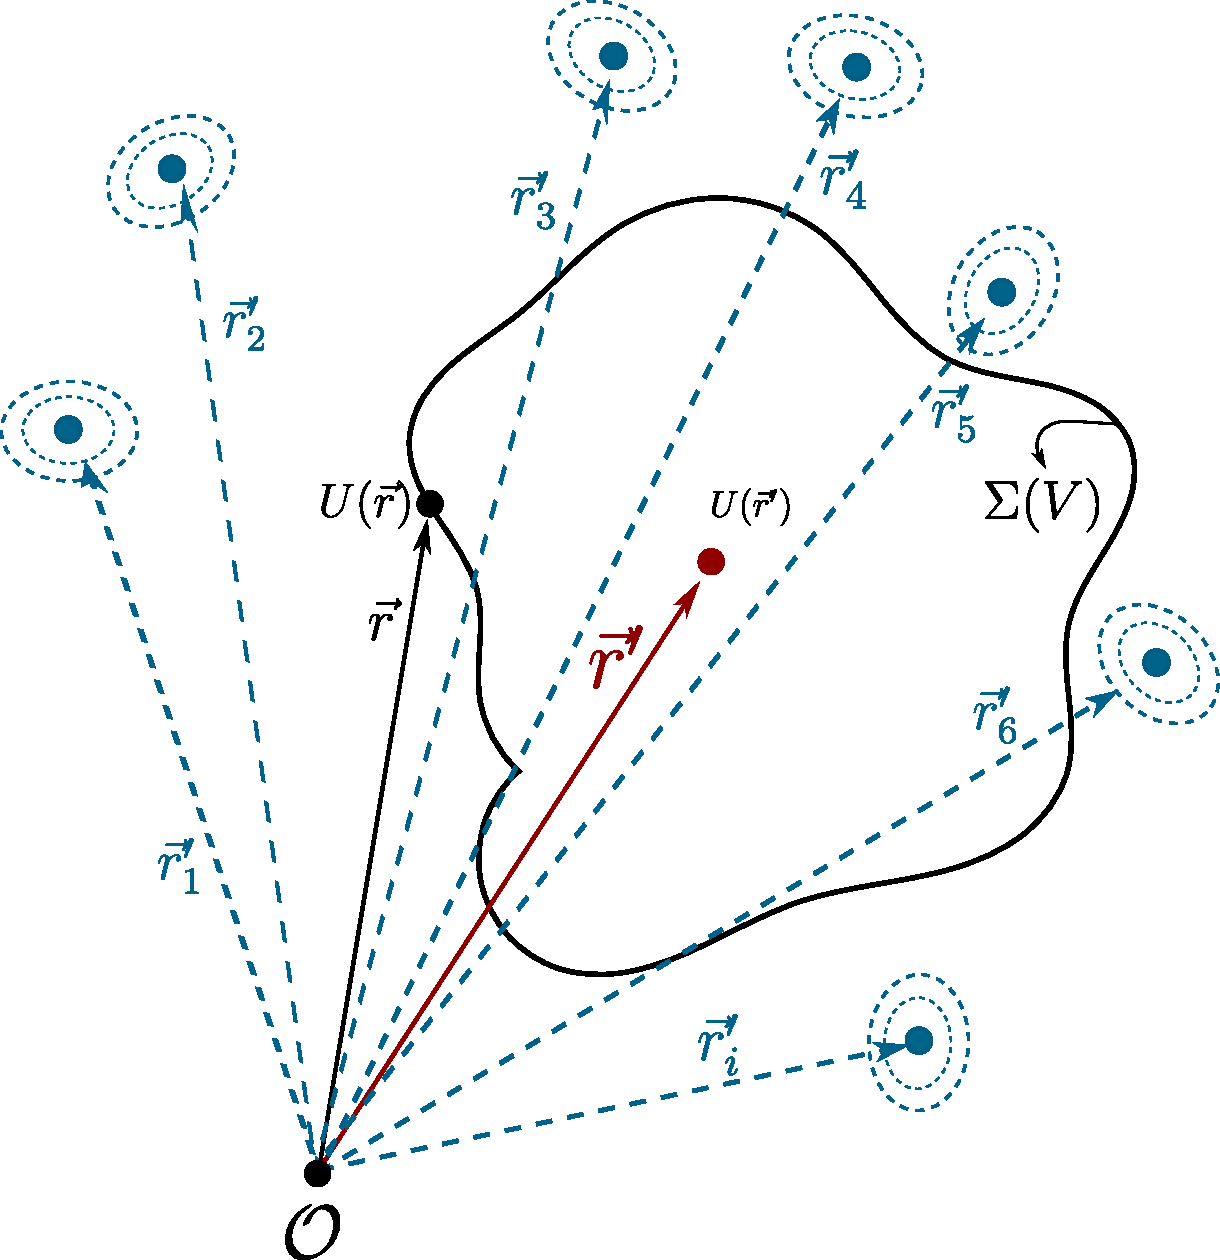
\includegraphics[width=0.7\linewidth]{Capitulo 1/Figuras/GreenImagenes}
			\caption{Sobre la frontera $\Sigma(V)$ se muestra la contribución de las componentes del campo $U(\vec{r})$; dentro de la región, el campo total se construye a partir de la contribución de todos los puntos de la frontera. Se pueden añadir infinitas cargas puntuales de Green de naturaleza de propagación arbitraria; la condición para la invariancia de la ecuación \eqref{eq:GreenHomogeneous} es que estas cargas imagen se encuentren fuera de $\Sigma(V)$.}
			\label{fig:greenimages}
		\end{figure}

		En este espíritu, la ecuación \eqref{eq:GreenHomogeneous} se convierte en
		\begin{equation}
			(\nabla^2 + k^2)G(\vec{r},\vec{r}') = -4\pi \delta(\vec{r}-\vec{r}') - 4\pi \sum_{i=1}^{\infty} \delta(\vec{r}-\vec{r}''_i).
		\end{equation}
		La solución explícita para un medio homogéneo de la ecuación \eqref{eq:GreenHomogeneous} es
		\begin{equation}
			\label{sol_Green}
			G(\vec{r}, \vec{r}') = \frac{e^{ik\|\vec{r} - \vec{r}'\|}}{\|\vec{r} - \vec{r}'\|},
		\end{equation}
		correspondiente a una onda esférica saliente centrada en $\vec{r}'$, como se demostrará en \eqref{eq:GreenSpherical}. Sustituyendo $G$ en la identidad de Green, y usando que la integral de volumen recoge el valor $-4\pi U(\vec{r}',\nu)$ debido a la delta, se obtiene
		\begin{equation}
			\label{green}
			U(\vec{r}', \nu) = -\frac{1}{4\pi} \oint_{\Sigma(V)} \left[ U(\vec{r}, \nu)\nabla G(\vec{r}, \vec{r}')- G(\vec{r}, \vec{r}')\nabla U(\vec{r}, \nu)  \right ] \cdot d\vec{\sigma},
		\end{equation}
		conocida como la fórmula integral de Helmholtz-Kirchhoff. Esta ecuación permite calcular $U(\vec{r}', \nu)$ en cualquier punto del volumen $V$ mediante una integral sobre su frontera $\Sigma(V)$.

		\begin{figure}[htbp]
			\centering
			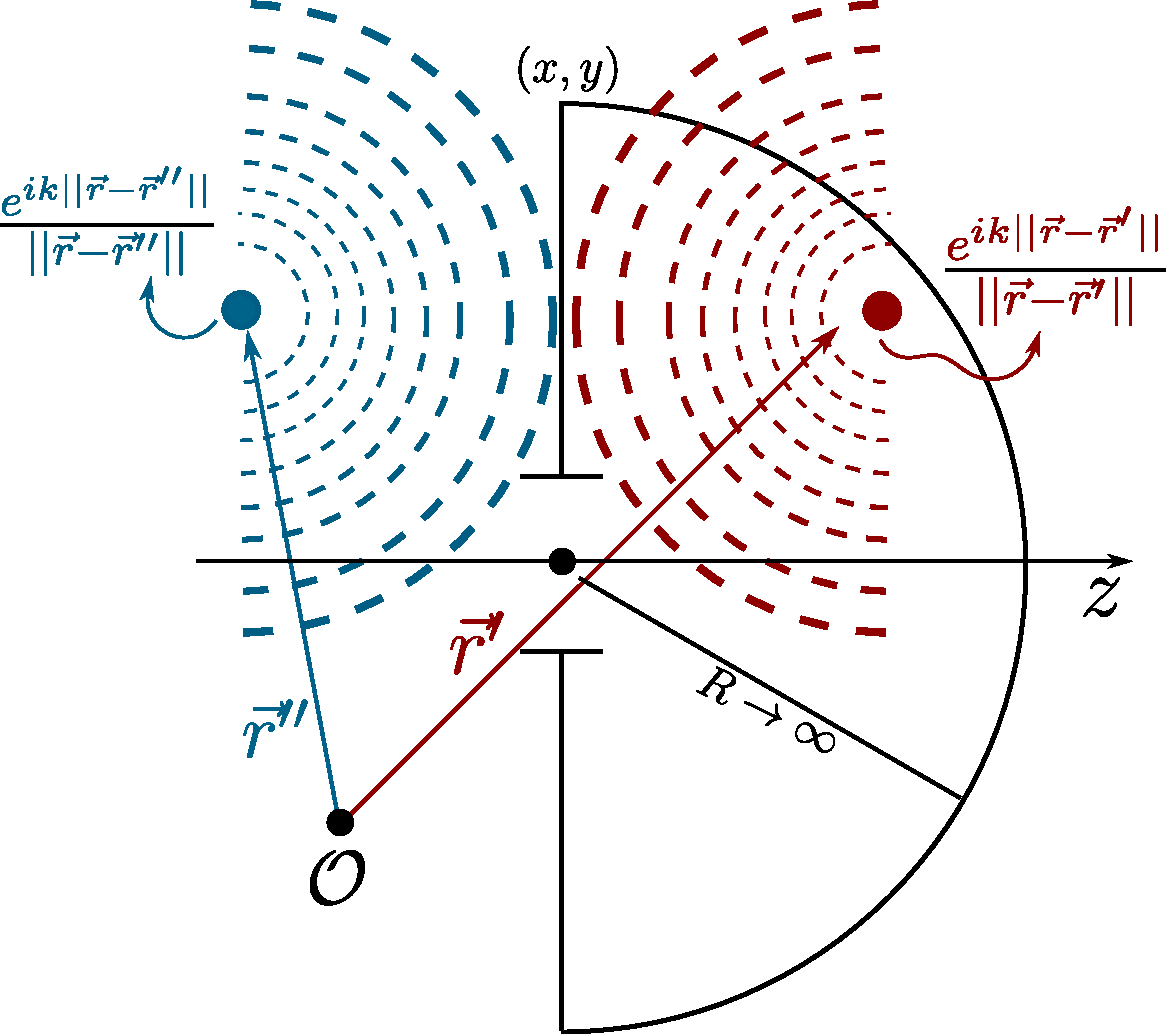
\includegraphics[width=0.7\linewidth]{Capitulo 1/Figuras/GreenPuntual}
			\caption{Representación de las funciones de Green para fuentes puntuales. Bajo estas condiciones de frontera, las funciones de Green se comportan como cargas puntuales, una imagen especular de la otra.}
			\label{fig:greenpoint}
		\end{figure}

		Antes de continuar, vale la pena notar que la naturaleza de carga puntual de las funciones de Green $G(\vec{r},\vec{r}')$ es un supuesto que se da por sentado; no existe, sin embargo, ninguna restricción sobre su naturaleza física. Como es bien sabido en la teoría electromagnética, las fuentes de radiación pueden tener cualquier volumen y forma, de modo que nuestro problema (Figura~\ref{fig:greenpoint}) puede generalizarse, como se muestra en la Figura~\ref{fig:greennonpoint}, y la ecuación diferencial para funciones de Green con volumen se leería
		\begin{equation}
			\left( \nabla^2 + k^2 \right)G(\vec{r},\vec{r}') = -4\pi \rho(\vec{r}-\vec{r}'_+) + 4\pi\rho(\vec{r}-\vec{r}'_-).
		\end{equation}

		\begin{figure}[htbp]
			\centering
			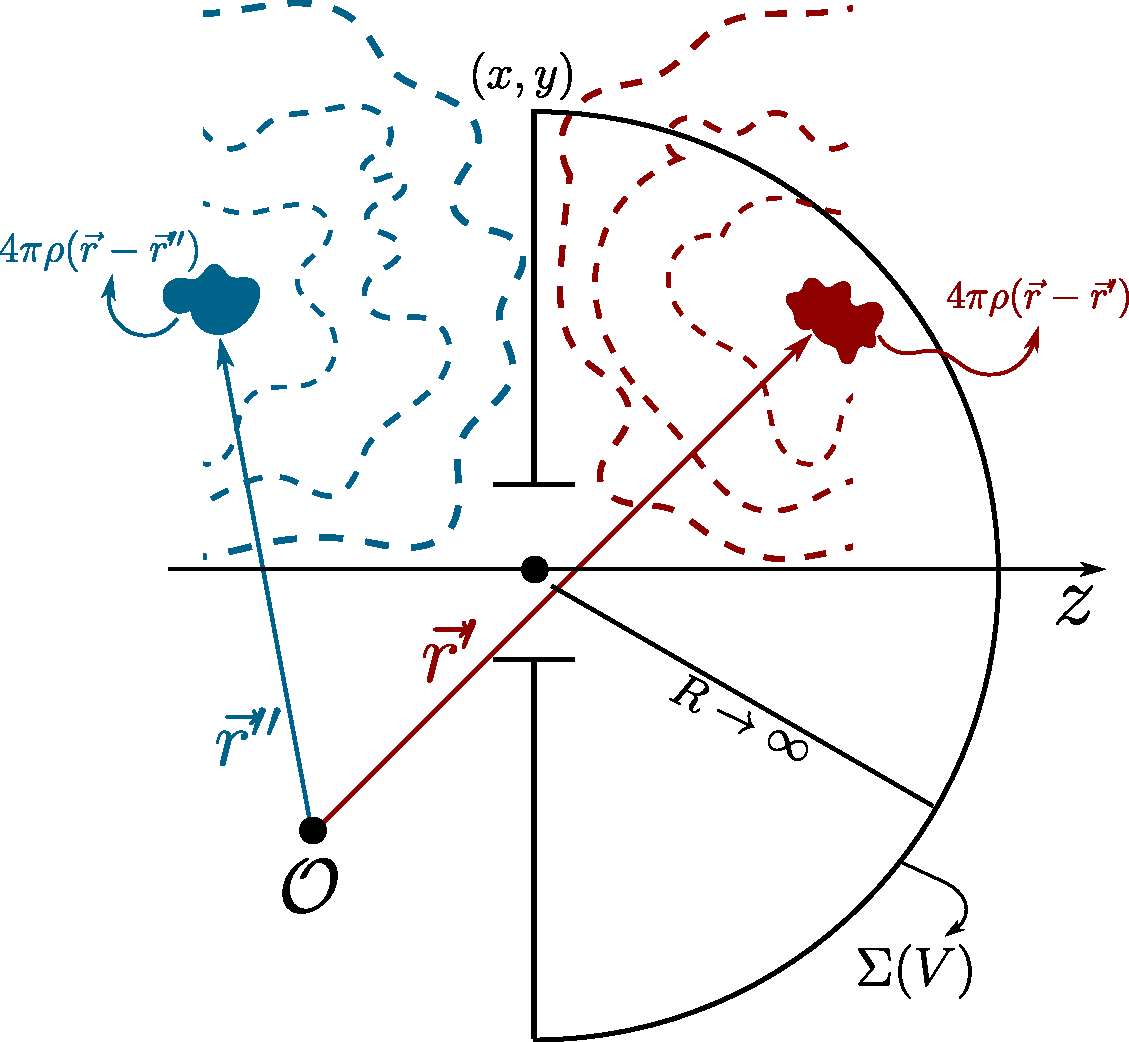
\includegraphics[width=0.7\linewidth]{Capitulo 1/Figuras/GreenNoPuntual}
			\caption{Representación de las funciones de Green para fuentes no puntuales. Bajo estas condiciones de frontera, las funciones de Green siguen comportándose como imágenes especulares, pero ahora con un volumen y una geometría dados; la única restricción sobre la emisión de estas fuentes es que, en la frontera $z=0$, el campo total debe anularse, como exigen las condiciones de Dirichlet supuestas.}
			\label{fig:greennonpoint}
		\end{figure}

		Continuemos con el desarrollo para funciones de Green puntuales. Para simplificar la evaluación de la integral, consideramos un volumen $V$ delimitado por un plano infinito $\Sigma_1$ ($z=0$) y una semiesfera $\Sigma_2$ de radio $R$ (véase la Figura~\ref{fig:greenpoint}). Cerrar la superficie en el infinito es legítimo solo si nada llega desde allí, y de nuevo esto es una decisión sobre el experimento y no una consecuencia de las matemáticas: excluye cualquier onda que converja sobre la abertura desde el lado lejano, que es precisamente lo que se dispone en el laboratorio al colocar toda fuente de luz detrás de la pantalla y al trabajar en una habitación oscurecida.

		\begin{Assumption}
			Ninguna radiación llega a la región de observación desde el infinito, siendo el campo sobre la semiesfera $\Sigma_{2}$ puramente saliente y obedeciendo la condición de radiación de Sommerfeld \eqref{eq:SommerfeldRadiation}, de modo que la contribución de $\Sigma_{2}$ se anula cuando $R\to\infty$.
		\end{Assumption}

		La fórmula de Helmholtz-Kirchhoff se reduce entonces a
		\begin{equation}
			U(\vec{r}', \nu) = -\frac{1}{4\pi} \int_{\Sigma_1} \left[U(\vec{r}, \nu)\frac{\partial G}{\partial n} -   G(\vec{r}, \vec{r}')\frac{\partial U}{\partial n} \right] d\sigma,
		\end{equation}
		donde $\frac{\partial}{\partial n} = \hat{n} \cdot \nabla$ denota la derivada normal. Sin embargo, esta formulación exige especificar simultáneamente $U$ y $\partial U/\partial n$ sobre $\Sigma_1$, lo cual sobredetermina el problema. Esta dificultad motiva la introducción de condiciones de frontera físicamente realistas, como las de Kirchhoff, para resolver la ambigüedad.

		Este problema se ve agravado por un teorema del análisis complejo, atribuido a Riemann, que afirma que si una función y su derivada normal se anulan en una región abierta de un plano, entonces la función debe ser idénticamente nula en todo el dominio. Esta restricción motiva la necesidad estratégica de eliminar uno de los términos en la integral de superficie de Helmholtz-Kirchhoff.

		La clave consiste en explotar los grados de libertad inherentes a la elección de la función de Green auxiliar $G$. Kirchhoff propuso inicialmente las condiciones de frontera intuitivas
		\begin{itemize}
			\item $U = 0$ fuera de la abertura sobre $\Sigma$ (campo bloqueado),
			\item $\partial U/\partial n = 0$ en las regiones opacas (derivada normal nula).
		\end{itemize}

		Aunque estas condiciones reproducían los resultados experimentales de la difracción, introducían inconsistencias matemáticas al violar el teorema de unicidad de Cauchy-Riemann. Poincaré mostró que tales supuestos generan contradicciones en las derivadas mixtas del campo. La resolución vino de Sommerfeld, quien redefinió $G$ por medio de una función de Green de doble capa (especular), garantizando que
		\begin{itemize}
			\item $G = 0$ sobre $\Sigma$ (condición de Dirichlet),
			\item $\partial G/\partial n$ permanece no singular,
		\end{itemize}

	eliminando así la redundancia en las condiciones de frontera y preservando la autoconsistencia del formalismo.

	El artificio de Sommerfeld elimina uno de los dos términos de frontera, pero no elimina la necesidad de conocer el que sobrevive. La fórmula de Rayleigh-Sommerfeld sigue requiriendo el valor de $U$ en cada punto del plano $\Sigma_{1}$, y ninguna teoría de la difracción puede suministrarlo, porque obtenerlo significaría resolver exactamente el problema electromagnético de la pantalla que precisamente buscábamos evitar. Lo que se hace en cambio es adivinarlo, y la conjetura es la de Kirchhoff. Descansa sobre dos idealizaciones separadas, una sobre el obstáculo y otra sobre el campo en él, y ambas merecen enunciarse como lo que son.

	\begin{Assumption}
		La pantalla es un obstáculo plano de espesor nulo, perfectamente opaco y perfectamente absorbente, cuyas propiedades materiales no desempeñan ningún papel en el problema y cuyos bordes no perturban el campo en su vecindad.
	\end{Assumption}

	\begin{Assumption}
		Sobre la abertura el campo coincide con el campo que existiría si la pantalla nunca se hubiera introducido, y sobre la parte opaca de la pantalla se anula idénticamente.
	\end{Assumption}

	El segundo de estos supuestos es el eslabón más débil de toda la construcción, y resulta instructivo ver por qué. Un campo que se anula en parte de un plano y coincide con una onda incidente suave en el resto es discontinuo en el borde de la abertura, por lo que no puede ser una solución exacta de la ecuación de Helmholtz; los valores de frontera que prescribimos son, estrictamente hablando, incompatibles con la ecuación que estamos resolviendo. El error queda confinado a un borde de unas pocas longitudes de onda de ancho alrededor del borde, razón por la cual la teoría funciona tan bien para aberturas de muchas longitudes de onda y falla para aberturas comparables con la longitud de onda.


	\subsection{La formulación de Rayleigh-Sommerfeld}

		Ya hemos usado dos veces la forma explícita \eqref{sol_Green} de la función de Green sin justificarla, y puesto que toda la construcción de Rayleigh-Sommerfeld descansa tanto en la forma de esa función como en la libertad de sumarle una segunda, este es el lugar para mostrar de dónde proviene.

		\begin{myteo}
			Sea $R = \|\vec{r}-\vec{r}'\|$. En un medio homogéneo, isótropo e ilimitado, la única solución de la ecuación de Green \eqref{eq:GreenHomogeneous} que transporta energía alejándose de la fuente es la onda esférica saliente
			\begin{equation}\label{eq:GreenSpherical}
				G(\vec{r},\vec{r}') = \frac{e^{ikR}}{R},
			\end{equation}
			fijándose su amplitud por la intensidad asignada al emisor puntual y quedando excluida la solución convergente por la condición de radiación.
		\end{myteo}

		La demostración tiene cuatro pasos, y cada uno de ellos es una afirmación física antes de ser una afirmación matemática. El primero es una cuestión de simetría. El medio es homogéneo e isótropo y la fuente es un único punto, de modo que, una vez colocado el origen en $\vec{r}'$, nada en el problema distingue una dirección del espacio de otra; la solución solo puede depender de la distancia $R$ a la fuente, y podemos escribir $G = G(R)$.

		El segundo paso consiste en resolver la ecuación lejos de la fuente, donde es homogénea. Para una función que depende únicamente de $R$, el laplaciano se reduce a
		\begin{equation}\label{eq:GreenRadialLaplacian}
			\nabla^{2}G = \frac{1}{R^{2}}\frac{d}{dR}\left(R^{2}\frac{dG}{dR}\right) = \frac{1}{R}\frac{d^{2}}{dR^{2}}\left(R\,G\right),
		\end{equation}
		donde la segunda forma corresponde a una identidad radial ya establecida al estudiar el laplaciano en coordenadas esféricas, y que sugiere de inmediato la sustitución $\chi(R) = R\,G(R)$. Con ella, la ecuación de Helmholtz homogénea se convierte en
		\begin{equation}\label{eq:RadialOscillator}
			\frac{d^{2}\chi}{dR^{2}} + k^{2}\chi = 0 ,
		\end{equation}
		que es la ecuación de un oscilador armónico en la variable $R$ y cuya solución general es $\chi = A\,e^{ikR} + B\,e^{-ikR}$. Deshaciendo la sustitución,
		\begin{equation}\label{eq:GreenGeneralRadial}
			G(R) = A\,\frac{e^{ikR}}{R} + B\,\frac{e^{-ikR}}{R},
		\end{equation}
		de modo que la amplitud de un campo monocromático con simetría esférica decae necesariamente como el inverso de la distancia. Esto no es un accidente del álgebra. La energía que atraviesa una esfera de radio $R$ es proporcional a $|G|^{2}R^{2}$, y solo con la dependencia $1/R$ esta cantidad resulta independiente de $R$, tal como exige la conservación de la energía en un medio transparente.

		El tercer paso selecciona entre los dos términos de \eqref{eq:GreenGeneralRadial}. Restaurando el factor temporal de la convención de Fourier adoptada en \eqref{eq.FT}, las dos soluciones se leen $e^{i(kR-\omega t)}/R$ y $e^{-i(kR+\omega t)}/R$, y sus superficies de fase constante obedecen respectivamente $R = ct + \text{const}$ y $R = -ct + \text{const}$. La primera se expande y la segunda se contrae. Nuestro punto es un emisor y no un sumidero, y la luz debe alejarse de él y nunca regresar, que es el contenido físico de la condición de radiación de Sommerfeld ya invocada al descartar la semiesfera $\Sigma_{2}$,
		\begin{equation}\label{eq:SommerfeldRadiation}
			\lim_{R\to\infty} R\left(\frac{\partial G}{\partial R} - ikG\right) = 0 .
		\end{equation}
		La onda convergente la viola, pues para ella el corchete se comporta como $-2ikB\,e^{-ikR}/R$ y el producto con $R$ no tiende a cero. Por lo tanto $B = 0$.

		El cuarto paso es el único en el que interviene la delta, y es el que fija la amplitud $A$. Integramos \eqref{eq:GreenHomogeneous} sobre la bola $B_{\varepsilon}$ de radio $\varepsilon$ centrada en la fuente, que es lo que produjo \eqref{eq:GreenFlux}. Con $G = A\,e^{ikR}/R$ el término de volumen está acotado por
		\begin{equation*}
			\left|k^{2}\int_{B_{\varepsilon}} G\, dV\right| = \left|4\pi A k^{2}\int_{0}^{\varepsilon} \frac{e^{ikR}}{R}\,R^{2}\,dR\right| \leq 2\pi |A|\,k^{2}\varepsilon^{2} \xrightarrow[\varepsilon\to 0]{} 0,
		\end{equation*}
		de modo que la singularidad de $G$ es lo suficientemente suave para ser integrable, y toda la intensidad de la fuente debe provenir del término de flujo. Puesto que $\partial G/\partial R = A\,e^{ikR}\left(ik/R - 1/R^{2}\right)$, y la esfera $\partial B_{\varepsilon}$ tiene área $4\pi\varepsilon^{2}$ con normal exterior $\hat{R}$,
		\begin{equation*}
			\oint_{\partial B_{\varepsilon}} \nabla G\cdot d\vec{\sigma} = 4\pi\varepsilon^{2}\,A\,e^{ik\varepsilon}\left(\frac{ik}{\varepsilon}-\frac{1}{\varepsilon^{2}}\right) = 4\pi A\,e^{ik\varepsilon}\left(ik\varepsilon - 1\right) \xrightarrow[\varepsilon\to 0]{} -4\pi A ,
		\end{equation*}
		y \eqref{eq:GreenFlux} da entonces $-4\pi A = -4\pi$, es decir $A = 1$, lo que demuestra \eqref{eq:GreenSpherical} y completa el argumento.

		El signo de la fuente merece un comentario, porque es la razón por la cual \eqref{eq:GreenHomogeneous} lleva $-4\pi$ y no $+4\pi$ en el lado derecho. El último paso de la demostración muestra que el flujo de $\nabla G$ que sale de una pequeña esfera es $-4\pi A$, de modo que una amplitud positiva $A$ exige una constante negativa en la ecuación; si hubiéramos escrito $+4\pi\delta(\vec{r}-\vec{r}')$ nos habríamos visto obligados a aceptar $A = -1$, es decir $G = -e^{ikR}/R$, y toda fórmula escrita a partir de \eqref{sol_Green} en adelante habría cambiado de signo. La convención adoptada aquí es la usada por Sommerfeld, Born y Wolf, y Goodman \citep{sommerfeld1954optics, born1999principles, goodman2005introduction}, y es la convención para la cual la integral de difracción resulta con la conocida constante $1/(i\lambda)$. Lo que el cálculo establece, más allá de la contabilidad de signos, es que la solución elemental es una onda esférica saliente centrada en el punto fuente cuya amplitud es inversamente proporcional a la distancia. Esta es la ondita de Huygens, ahora obtenida en lugar de supuesta.

		Volviendo a la ecuación \eqref{green} y eligiendo la condición de Dirichlet para la función $G$, el segundo término del integrando desaparece y nos queda
		\begin{equation}
			\label{psi_expr}
			U(\vec{r}', \nu) = -\frac{1}{4\pi} \int_{\Sigma_1} \left[U(\vec{r}, \nu) \nabla G \cdot\hat{n}\right] d\sigma .
		\end{equation}
		Aquí $\hat{n}$ es la normal que apunta \textit{hacia afuera} de $V$, y como $V$ es el semiespacio $z>0$, sobre el plano $\Sigma_{1}$ esa normal apunta hacia abajo, $\hat{n} = -\hat{z}$. Vale la pena escribir esto explícitamente, porque es el signo que con mayor facilidad se pierde en toda la construcción,
		\begin{equation}\label{eq:RSnormal}
			U(\vec{r}', \nu) = \frac{1}{4\pi} \int_{\Sigma_1} U(\vec{r}, \nu)\,\nabla G \cdot\hat{z}\; d\sigma .
		\end{equation}
		Dada la superficie de integración considerada, podemos expresar \eqref{sol_Green} como
		\begin{equation}
			\label{sol_Green_RS}
			G(\vec{r}, \vec{r}') = \frac{e^{ik\|\vec{r} - \vec{r}'\|}}{\|\vec{r} - \vec{r}'\|} - \frac{e^{ik\|\vec{r} - \vec{r}''\|}}{\|\vec{r} - \vec{r}''\|},
		\end{equation}
		\noindent donde
		\begin{align}
			\|\vec{r} - \vec{r}''\| &= \|\vec{r} - \vec{r}'\|, \qquad x'' = x', \quad y'' = y', \quad z'' = -z',
		\end{align}
		puesto que $\vec{r}''$ es la imagen especular de $\vec{r}'$ respecto al plano $\Sigma_1$.

		Que \eqref{sol_Green_RS} sea una función de Green legítima se verifica de inmediato con el teorema recién demostrado. El punto de observación $\vec{r}'$ se encuentra en el semiespacio $z>0$, de modo que su imagen $\vec{r}''$ se encuentra en $z<0$, fuera del volumen $V$; dentro de $V$, el segundo término es entonces una solución perfectamente regular de la ecuación de Helmholtz homogénea, y sumarlo no altera ni la fuente en $\vec{r}'$ ni el valor de la integral de volumen, de acuerdo con la libertad discutida después de \eqref{eq:GreenHomogeneous}. Sobre el plano $\Sigma_{1}$, en cambio, todo punto es equidistante de $\vec{r}'$ y de $\vec{r}''$, de modo que las dos ondas esféricas llegan allí con la misma amplitud y la misma fase y se cancelan idénticamente, dando $G = 0$ en todo $\Sigma_{1}$. Esta es la condición de Dirichlet que buscábamos, obtenida mediante el mismo método de imágenes que resuelve el interferómetro de Michelson, y es lo que elimina el término en $\partial U/\partial n$ de \eqref{green} y con él la sobredeterminación de las condiciones de frontera de Kirchhoff.

		Todo lo que \eqref{eq:RSnormal} sigue requiriendo es la derivada axial de $G$ sobre el plano. Este es el único cálculo de la sección, y puesto que un signo perdido aquí cambia el signo de toda fórmula de difracción del resto del capítulo, lo llevaremos a cabo sin omitir un solo paso. Para aligerar la notación escribimos
		\begin{equation}\label{eq:RSDistances}
			r_{1} = \|\vec{r}-\vec{r}'\|, \qquad r_{2} = \|\vec{r}-\vec{r}''\|, \qquad f(\rho) = \dfrac{e^{ik\rho}}{\rho},
		\end{equation}
		de modo que \eqref{sol_Green_RS} se lee simplemente $G = f(r_{1}) - f(r_{2})$.

		\textit{Primer paso: la derivada de $f$.} Derivando el cociente,
		\begin{equation}\label{eq:RSderivf}
			\dfrac{df}{d\rho} = \dfrac{\left(ik\,e^{ik\rho}\right)\rho - e^{ik\rho}}{\rho^{2}} = \dfrac{e^{ik\rho}}{\rho}\left(ik - \dfrac{1}{\rho}\right) = \left(ik-\dfrac{1}{\rho}\right)f(\rho).
		\end{equation}

		\textit{Segundo paso: el gradiente de una distancia.} Con $\vec{r} = (x,y,z)$ el punto de integración y $\vec{r}' = (x',y',z')$ fijo,
		\begin{equation}\label{eq:RSr1}
			r_{1} = \left[(x-x')^{2}+(y-y')^{2}+(z-z')^{2}\right]^{1/2},
		\end{equation}
		y derivando respecto a $z$, que es la única componente que necesitaremos,
		\begin{equation}\label{eq:RSdr1dz}
			\dfrac{\partial r_{1}}{\partial z} = \dfrac{1}{2}\,\dfrac{2\left(z-z'\right)}{\left[(x-x')^{2}+(y-y')^{2}+(z-z')^{2}\right]^{1/2}} = \dfrac{z-z'}{r_{1}} ,
		\end{equation}
		el mismo cálculo con $\vec{r}''$ en lugar de $\vec{r}'$ da $\partial r_{2}/\partial z = (z-z'')/r_{2}$. Realizado para las tres componentes a la vez, estos dos resultados se leen $\nabla r_{1} = (\vec{r}-\vec{r}')/r_{1}$ y $\nabla r_{2} = (\vec{r}-\vec{r}'')/r_{2}$: el gradiente de una distancia es el vector unitario que apunta alejándose del centro desde el cual se mide la distancia.

		\textit{Tercer paso: el gradiente de $G$.} Aplicando la regla de la cadena a cada término y usando \eqref{eq:RSderivf},
		\begin{equation}\label{eq:RSgradG}
			\nabla G = \left(ik-\dfrac{1}{r_{1}}\right)\dfrac{e^{ikr_{1}}}{r_{1}}\,\dfrac{\vec{r}-\vec{r}'}{r_{1}} \;-\; \left(ik-\dfrac{1}{r_{2}}\right)\dfrac{e^{ikr_{2}}}{r_{2}}\,\dfrac{\vec{r}-\vec{r}''}{r_{2}} .
		\end{equation}

		\textit{Cuarto paso: la proyección sobre el eje.} Tomando el producto escalar de \eqref{eq:RSgradG} con $\hat{z}$, lo cual equivale a conservar la tercera componente de cada uno de los dos vectores,
		\begin{equation}\label{eq:RSgradGz}
			\nabla G\cdot\hat{z} = \left(ik-\dfrac{1}{r_{1}}\right)\dfrac{e^{ikr_{1}}}{r_{1}}\,\dfrac{z-z'}{r_{1}} \;-\; \left(ik-\dfrac{1}{r_{2}}\right)\dfrac{e^{ikr_{2}}}{r_{2}}\,\dfrac{z-z''}{r_{2}} .
		\end{equation}

		\textit{Quinto paso: evaluación sobre el plano.} La integral de \eqref{eq:RSnormal} se extiende sobre $\Sigma_{1}$, de modo que \eqref{eq:RSgradGz} solo se necesita en $z=0$. Allí las dos distancias coinciden, $r_{1} = r_{2} \equiv r$, que es la relación especular ya usada, y los dos desplazamientos axiales son
		\begin{equation}\label{eq:RSopposite}
			\left.\left(z-z'\right)\right|_{z=0} = -z', \qquad \left.\left(z-z''\right)\right|_{z=0} = -z'' = z' ,
		\end{equation}
		porque $z'' = -z'$. Este es el punto crucial de todo el cálculo: la fuente y su imagen se encuentran en lados opuestos del plano, de modo que sus cosenos directores axiales son iguales en magnitud y opuestos en signo. Sustituyendo \eqref{eq:RSopposite} en \eqref{eq:RSgradGz}, el factor común $\left(ik-1/r\right)e^{ikr}/r$ puede extraerse y lo que queda es una diferencia de dos números opuestos,
		\begin{equation}\label{eq:RSgradGplane}
			\left.\nabla G\cdot\hat{z}\right|_{\Sigma_{1}} = \left(ik-\dfrac{1}{r}\right)\dfrac{e^{ikr}}{r}\left[\dfrac{-z'}{r} - \dfrac{z'}{r}\right] = -\,\dfrac{2z'}{r}\left(ik-\dfrac{1}{r}\right)\dfrac{e^{ikr}}{r} .
		\end{equation}
		El factor dos merece un comentario. El signo menos que separa los dos términos de \eqref{sol_Green_RS} es lo que hace que las dos ondas esféricas se cancelen sobre el plano; ese mismo signo menos, combinado con los cosenos directores opuestos de \eqref{eq:RSopposite}, hace que sus derivadas axiales se sumen. La función de Green de Dirichlet se anula sobre $\Sigma_{1}$ y tiene allí exactamente el doble de la derivada normal de una única ondita, que es la huella analítica del hecho de que la pantalla se comporta como un espejo perfecto.

		\textit{Sexto paso: el factor de oblicuidad.} Solo resta nombrar la cantidad geométrica $z'/r$. Sea $\theta$ el ángulo entre el eje $\hat{z}$ y el vector $\vec{r}\,'-\vec{r}$ que va del punto de la abertura al punto de observación, de modo que
		\begin{equation}\label{eq:RSobliquity}
			\cos\theta = \hat{z}\cdot\dfrac{\vec{r}\,'-\vec{r}}{\|\vec{r}\,'-\vec{r}\|} = \dfrac{z'}{r} ,
		\end{equation}
		cantidad que es positiva porque el punto de observación se encuentra en $z>0$, y que es igual a uno para un punto de la abertura situado sobre el eje de observación. Con esta notación, \eqref{eq:RSgradGplane} adopta su forma final,
		\begin{equation}\label{eq:RSnormalDerivative}
			\left.\nabla G\cdot\hat{z}\right|_{\Sigma_{1}} = -2\left[ik-\dfrac{1}{r}\right]\dfrac{e^{ikr}}{r}\,\cos\theta .
		\end{equation}
		Es esencial tener presente desde cuál de los dos vectores se mide el ángulo. Si hubiéramos escrito el coseno director de $\vec{r}-\vec{r}'$, que apunta desde el punto de observación de vuelta a la abertura, habríamos obtenido el número opuesto, y la integral de difracción habría resultado con el signo equivocado.

		Sustituyendo \eqref{eq:RSnormalDerivative} en \eqref{eq:RSnormal}, los dos factores de dos se combinan con el $4\pi$ y obtenemos
		\begin{equation}\label{eq:RSexact}
			U(\vec{r}',\nu) = -\dfrac{1}{2\pi} \int_{\Sigma} U(\vec{r},\nu) \left[ik - \dfrac{1}{\|\vec{r} - \vec{r}'\|} \right] \dfrac{e^{ik\|\vec{r}-\vec{r}'\|}}{\|\vec{r}-\vec{r}'\|} \cos\theta\,d\sigma .
		\end{equation}
		La ecuación \eqref{eq:RSexact} es exacta dentro de la teoría escalar, y es la última expresión de este capítulo de la que puede decirse esto. Para llevarla a la forma en que efectivamente se usa, se descarta el término $1/\|\vec{r}-\vec{r}'\|$ frente a $k$, lo cual solo es lícito cuando el punto de observación se encuentra a muchas longitudes de onda de la abertura. Para luz visible y distancias de laboratorio, la razón descartada $\lambda/(2\pi\|\vec{r}-\vec{r}'\|)$ es del orden de $10^{-7}$, de modo que la aproximación es excelente, pero es una aproximación y no una identidad.

		\begin{Assumption}
			El punto de observación se encuentra a muchas longitudes de onda de todo punto de la abertura, $\|\vec{r}-\vec{r}'\| \gg \lambda$, de modo que el término de campo cercano $1/\|\vec{r}-\vec{r}'\|$ es despreciable frente al número de onda $k$.
		\end{Assumption}

		Con ello obtenemos
		\begin{equation}\label{eq:RSfinal}
			U(\vec{r}',\nu) = -\dfrac{ik}{2\pi} \int_{\Sigma} U(\vec{r},\nu)\dfrac{e^{ik\|\vec{r}-\vec{r}'\|}}{\|\vec{r}-\vec{r}'\|} \cos\theta\,d\sigma = \dfrac{1}{i\lambda} \int_{\Sigma} U(\vec{r},\nu)\dfrac{e^{ik\|\vec{r}-\vec{r}'\|}}{\|\vec{r}-\vec{r}'\|} \cos\theta\,d\sigma,
		\end{equation}
		donde la última igualdad no es otra cosa que $-ik/2\pi = -i/\lambda = 1/(i\lambda)$. Esta es una expresión matemática que encarna el principio de Huygens-Fresnel: como puede apreciarse, hay una onda esférica por cada punto de la superficie de integración, ponderada por el factor de oblicuidad $\cos\theta$ y por la constante $1/(i\lambda)$, que es la constante que Fresnel tuvo que postular y que la derivación ahora entrega, con avance de cuarto de onda y $1/\lambda$ incluidos.

\section{La aproximación de Fresnel}

Partiendo del campo
\begin{align}
	U(\vec{r}') = -\frac{ik}{2\pi}\int_{\Sigma} U(\vec{r}) \frac{e^{ik \left\| \vec{r} - \vec{r}' \right\|}}{\left\| \vec{r} - \vec{r}' \right\|} \cos\theta \, \mathrm{d}\sigma,
\end{align}
es posible llevar a cabo la llamada aproximación de campo medio, o de Fresnel. La expansión sobre la que descansa es de tipo binomial, y una serie binomial solo puede truncarse cuando la cantidad expandida es pequeña; aquí esa cantidad es la razón entre la separación transversal y la distancia de propagación, de modo que truncar equivale a confinar todo el problema a un cono estrecho alrededor del eje óptico.

\begin{Assumption}
	Las dimensiones transversales de la abertura y de la región de observación son pequeñas comparadas con la distancia de propagación $z'$, y el término cuártico omitido en la expansión contribuye con una fase muy por debajo de un radián, $k\left[(x-x')^{2}+(y-y')^{2}\right]^{2}/8z'^{3} \ll 1$.
\end{Assumption}

Para ello recordamos que la integración se extiende sobre el plano $\Sigma_{1}$, en el cual $z=0$, de modo que la separación axial entre los dos puntos es la coordenada $z'$ del punto de observación por sí sola,
\begin{align}
	\label{aprox_r}
	\|\vec{r}-\vec{r}'\| &= \left.\left[(x-x')^2 + (y-y')^2 + (z-z')^2\right]^{1/2}\right|_{z=0} \notag \\
	&= \left[(x-x')^2 + (y-y')^2 + z'^2\right]^{1/2} \notag \\
	&= z'\left(1 + \dfrac{(x-x')^2 + (y-y')^2}{z'^2} \right)^{1/2} \notag \\
	&\approx z' + \dfrac{(x-x')^2+(y-y')^2}{2z'}.
\end{align}
Es $z'$, y no $z$, lo que mide la distancia de propagación. La abertura se encuentra en el origen del eje y es el punto de observación el que se desplaza, lo cual es la misma convención que produjo el factor de oblicuidad $\cos\theta = z'/r$ de \eqref{eq:RSobliquity} y la evaluación en $z=0$ de \eqref{eq:RSopposite}. Fijar $z'=0$ y factorizar $z$ en su lugar colocaría el punto de observación sobre la pantalla y haría que la distancia de propagación se anulara idénticamente.
Resulta claro que, para el factor $\dfrac{1}{\|\vec{r}- \vec{r}'\|}$, basta una expansión hasta el primer término de \eqref{aprox_r}; esto no basta, sin embargo, para el factor $e^{ik \left\| \vec{r} - \vec{r}' \right\|}$, ya que este último tiene comportamiento oscilatorio en su dominio, de modo que se requieren ambos términos. Los dos factores se tratan, por lo tanto, con distintos grados de precisión, y esa asimetría es en sí misma una hipótesis: presupone que un error de una fracción de longitud de onda, inofensivo en una amplitud que varía lentamente, es fatal en una fase, lo cual es cierto precisamente porque $k$ es enorme en la escala de la abertura.

\begin{Assumption}
	En la amplitud, la distancia puede reemplazarse por la separación axial, $\|\vec{r}-\vec{r}'\| \approx z'$, mientras que en la fase debe conservarse el término cuadrático de \eqref{aprox_r}.
\end{Assumption}

Tomamos además, para el factor de oblicuidad \eqref{eq:RSobliquity}, $\cos\theta = \dfrac{z'}{\|\vec{r} - \vec{r} '\|} \approx 1$, lo cual es lícito en el régimen paraxial porque el punto de observación se encuentra entonces cerca del eje.

\begin{Assumption}
	El factor de oblicuidad es unitario, $\cos\theta \approx 1$, formando toda dirección de interés un ángulo pequeño con el eje óptico.
\end{Assumption}

En este espíritu, obtenemos una expresión para el campo de la forma
\begin{equation}
	\label{Fresnel}
	U(\vec{r}') = \dfrac{e^{ikz'}}{i\lambda z'} \int U(\vec{r}) \exp \left(\dfrac{ik}{2z'} ((x-x')^2 + (y-y')^2) \right) d\sigma,
\end{equation}
que describe la propagación o difracción del campo electromagnético en el régimen de Fresnel. La constante $1/(i\lambda z')$, heredada de \eqref{eq:RSfinal}, es aquella para la cual el núcleo de \eqref{Fresnel} tiende a $\delta(\vec{r}-\vec{r}\,')$ cuando $z'\to 0$, de modo que una propagación a distancia nula deja el campo inalterado; esta es la comprobación que fija el signo sin lugar a dudas. Vale la pena subrayar que la ecuación \eqref{Fresnel} describe una onda parabólica, y aunque, al menos conceptualmente, tal propagación es válida para un campo medio, en la práctica ha resultado más que suficiente para distancias suficientemente cortas.

	\subsection{Ejemplo: difracción de Fraunhofer entre dos esferas confocales}

		\textit{Partiendo de la integral de Fresnel \eqref{Fresnel}, mostrar que entre dos esferas confocales se obtiene difracción de Fraunhofer.}

		Ante todo conviene expandir el cuadrado en el exponente de \eqref{Fresnel}. Escribiendo $r^{2} = x^{2}+y^{2}$ para el radio transversal en el plano emisor y $r'^{2} = x'^{2}+y'^{2}$ para el del plano receptor,
		\begin{equation}\label{eq:ExpandFresnelSquare}
			(x-x')^{2} + (y-y')^{2} = r^{2} + r'^{2} - 2\left(xx'+yy'\right),
		\end{equation}
		de modo que la integral de Fresnel se separa en tres factores,
		\begin{equation}\label{eq:FresnelThreeFactors}
			U(\vec{r}\,') = \dfrac{e^{ikz'}}{i\lambda z'}\int U(\vec{r})\,
			e^{\frac{ik}{2z'}r^{2}}\;
			e^{\frac{ik}{2z'}r'^{2}}\;
			e^{-\frac{ik}{z'}\left(xx'+yy'\right)}\,d\sigma .
		\end{equation}
		El último factor ya es el núcleo de una transformación de Fourier. El obstáculo es el par de factores cuadráticos, y todo el sentido del ejercicio es que no son obstáculo en absoluto si se acepta leer el campo sobre una superficie curva en lugar de sobre un plano.

		Consideremos un casquete esférico tangente a un plano transversal en el eje óptico, con su centro de curvatura sobre el eje a la distancia con signo $c$ desde el vértice, contada positiva en la dirección de propagación. El punto del casquete en la posición transversal $\vec{r}$ está desplazado axialmente respecto al plano tangente por la sagita
		\begin{align*}
			& \delta(r) = c - \operatorname{sgn}(c)\sqrt{c^{2}-r^{2}} = c - \operatorname{sgn}(c)\,|c|\sqrt{1-\dfrac{r^{2}}{c^{2}}} \approx {\color{red}c} - {\color{red}c}\left(1 - \dfrac{r^{2}}{2c^{2}}\right),
		\end{align*}
		donde usamos $\operatorname{sgn}(c)\,|c| = c$ y expandimos la raíz a primer orden, que es la misma expansión paraxial ya realizada en \eqref{aprox_r}. Los dos términos en rojo se cancelan y queda
		\begin{equation}\label{eq:ConfocalSagitta}
			\delta(r) = \dfrac{r^{2}}{2c}.
		\end{equation}
		Puesto que un campo que se propaga en la dirección positiva adquiere el factor $e^{ik\delta}$ a lo largo de un desplazamiento axial $\delta$, el campo leído sobre el casquete y el campo leído sobre el plano tangente están relacionados por
		\begin{equation}\label{eq:ConfocalRule}
			u_{\text{cap}}(\vec{r}) = U(\vec{r})\exp\left(\dfrac{ik\,r^{2}}{2c}\right).
		\end{equation}

		Se dice que dos esferas son \textit{confocales} cuando cada una tiene su centro de curvatura en el vértice de la otra. Sea entonces $\mathcal{A}$ el casquete tangente al plano emisor $\mathcal{P}$ en el vértice $O$ y centrado en $O'$, y sea $\mathcal{F}$ el casquete tangente al plano receptor $\mathcal{Q}$ en el vértice $O'$ y centrado en $O$, como se muestra en la Figura~\ref{fig:ConfocalSpheres}. Ambos radios son entonces iguales a la distancia de propagación, y con la convención de signos de \eqref{eq:ConfocalRule} las dos distancias con signo son
		\begin{equation}\label{eq:ConfocalRadii}
			c_{\mathcal{A}} = +z', \qquad c_{\mathcal{F}} = -z',
		\end{equation}
		siendo la segunda negativa porque el centro de $\mathcal{F}$ se encuentra aguas arriba de su propio vértice.

		\begin{figure}[!ht]
			\centering
			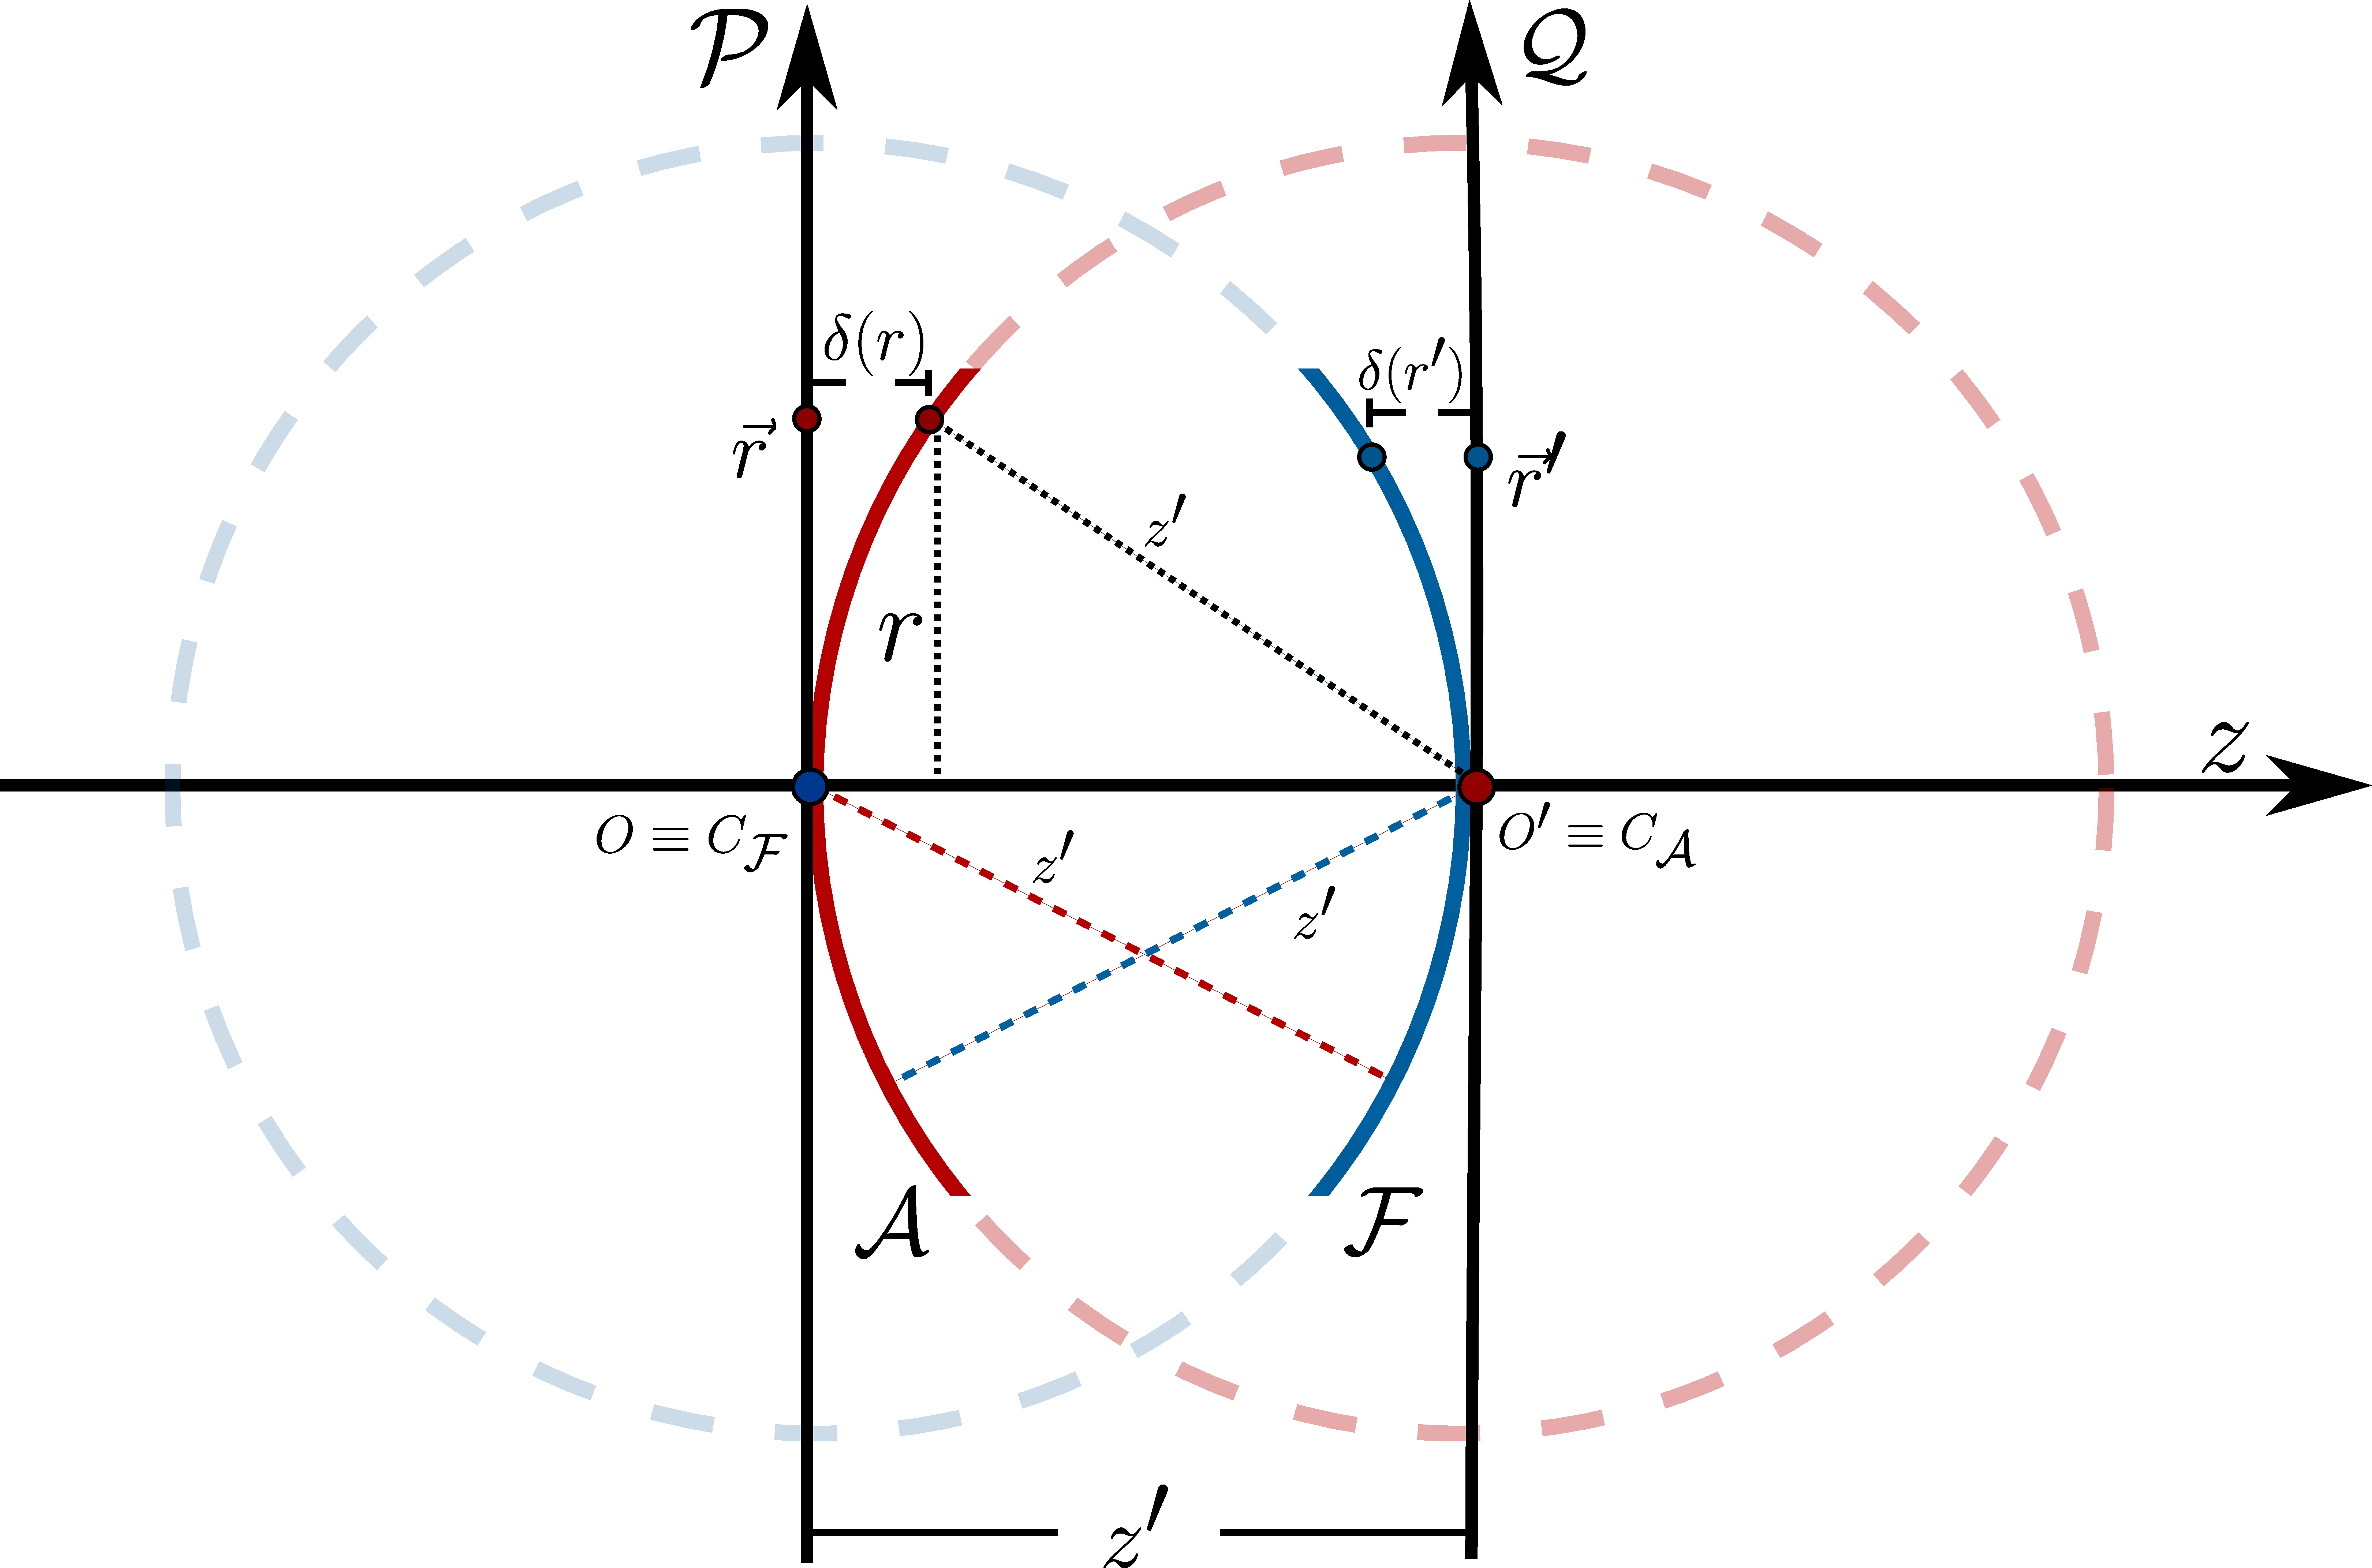
\includegraphics[width=0.7\textwidth]{Capitulo 1/Figuras/ConfocalSpheres.pdf}
			\caption{Geometría de las dos esferas confocales. El casquete $\mathcal{A}$ es tangente
			al plano emisor $\mathcal{P}$ en el vértice $O$ y tiene su centro de curvatura en
			$O'$, mientras que el casquete $\mathcal{F}$ es tangente al plano receptor $\mathcal{Q}$ en
			$O'$ y tiene su centro de curvatura en $O$, de modo que ambos radios son iguales a la distancia de
			propagación $z'$. Leída sobre estas dos superficies, la propagación de Fresnel se reduce a una
			transformación de Fourier exacta, que en el lenguaje de la transformada fraccionaria de Fourier
			de la Sección~\ref{sec:FrFT} corresponde al orden $\alpha = \pi/2$.}
			\label{fig:ConfocalSpheres}
		\end{figure}

		Aplicando \eqref{eq:ConfocalRule} en cada lado con los radios \eqref{eq:ConfocalRadii},
		\begin{equation}\label{eq:ConfocalReferring}
			U(\vec{r}) = u_{\mathcal{A}}(\vec{r})\,e^{-\frac{ik}{2z'}r^{2}}, \qquad
			u_{\mathcal{F}}(\vec{r}\,') = U(\vec{r}\,')\,e^{-\frac{ik}{2z'}r'^{2}} ,
		\end{equation}
		y sustituyendo ambas relaciones en \eqref{eq:FresnelThreeFactors},
		\begin{align*}
			& u_{\mathcal{F}}(\vec{r}\,') = \dfrac{e^{ikz'}}{i\lambda z'}\;
			{\color{red}e^{-\frac{ik}{2z'}r'^{2}}}\;{\color{red}e^{\frac{ik}{2z'}r'^{2}}}
			\int u_{\mathcal{A}}(\vec{r})\;
			{\color{red}e^{-\frac{ik}{2z'}r^{2}}}\;{\color{red}e^{\frac{ik}{2z'}r^{2}}}\;
			e^{-\frac{ik}{z'}\left(xx'+yy'\right)}\,d\sigma ,
		\end{align*}
		donde las cuatro exponenciales en rojo se cancelan en pares, ya que en cada par los dos exponentes son opuestos. Nos queda
		\begin{equation}\label{eq:ConfocalResult}
			\boxed{\;u_{\mathcal{F}}(\vec{r}\,') = \dfrac{e^{ikz'}}{i\lambda z'}\int u_{\mathcal{A}}(\vec{r})\,
			\exp\left[-\dfrac{ik}{z'}\left(xx'+yy'\right)\right]d\sigma ,\;}
		\end{equation}
		que es exactamente la expresión de Fraunhofer \eqref{Fraunhofer} \textit{sin el factor de curvatura}. Esto demuestra la afirmación.

		Son pertinentes tres comentarios, porque el resultado es más fuerte de lo que parece.

		En la derivación de \eqref{Fraunhofer} el factor $e^{ikr^{2}/2z'}$ fue \textit{despreciado} apelando al campo lejano. Aquí no ha sido despreciado, ha sido \textit{absorbido} por la elección de la superficie de referencia, y \eqref{eq:ConfocalResult} es por lo tanto exacta dentro de la aproximación de Fresnel, para cualquier distancia de propagación $z'$. La lección es que la difracción de Fraunhofer no es en realidad un régimen de distancias sino un enunciado sobre geometría: es lo que parece la propagación de Fresnel cuando el campo se lee sobre dos esferas confocales. El factor de curvatura que sobrevive fuera de la integral en \eqref{Fraunhofer} no es sino el precio de insistir en leer el campo sobre un plano, y esta es precisamente la interpretación anticipada en la Figura~\ref{fig:cardinals}.

		Introduciendo la frecuencia espacial asociada al punto de observación,
		\begin{equation}\label{eq:ConfocalFrequency}
			\vec{\nu} = \dfrac{\vec{r}\,'}{\lambda z'}, \qquad \dfrac{k}{z'}\left(xx'+yy'\right) = \dfrac{2\pi}{\lambda z'}\,\vec{r}\cdot\vec{r}\,' = 2\pi\,\vec{r}\cdot\vec{\nu},
		\end{equation}
		la ecuación \eqref{eq:ConfocalResult} se convierte en
		\begin{equation}\label{eq:ConfocalFourier}
			u_{\mathcal{F}}(\lambda z'\,\vec{\nu}) = \dfrac{e^{ikz'}}{i\lambda z'}\,\widehat{u_{\mathcal{A}}}(\vec{\nu}), \qquad \widehat{u_{\mathcal{A}}}(\vec{\nu}) = \int u_{\mathcal{A}}(\vec{r})\,e^{-2\pi i\,\vec{r}\cdot\vec{\nu}}\,d\sigma ,
		\end{equation}
		de modo que la coordenada de observación sobre la esfera $\mathcal{F}$ es, salvo por el factor de escala $\lambda z'$, la frecuencia espacial del campo sobre la esfera $\mathcal{A}$. Este es el sentido preciso en el cual un sistema difractante realiza un análisis de Fourier del objeto, la afirmación a la que Abbe había llegado cualitativamente en 1873 \citep{abbe1873beitrage}.

		Las únicas aproximaciones usadas son las ya contenidas en \eqref{Fresnel} junto con la expansión a primer orden \eqref{eq:ConfocalSagitta} de la sagita, de modo que el resultado se mantiene mientras la región iluminada satisfaga $r_{\max}\ll z'$, que es la condición para que los casquetes no se aparten apreciablemente de sus planos tangentes. Cuando esto deja de cumplirse hay que abandonar la descripción paraxial, tal como se señala al final de la siguiente sección.

		Por último, vale la pena registrar que este ejemplo es la primera instancia de un hecho mucho más general. Nada obliga a que las dos esferas de referencia sean confocales, y si se les da un radio común $R$ distinto de $z'$, los dos factores cuadráticos ya no se cancelan sino que se combinan en un chirp, y la propagación se convierte en una transformada fraccionaria de Fourier de un orden fijado por la razón $z'/R$. El caso confocal aquí tratado es el orden particular $\alpha = \pi/2$. Este es el tema de la Sección~\ref{sec:FrFT}.

\section{La aproximación de Fraunhofer}

Finalmente, a partir de la expresión \eqref{Fresnel} puede llevarse a cabo una segunda aproximación, correspondiente al campo lejano o régimen de Fraunhofer, en el cual las distancias de observación son considerablemente mayores que el área sobre la cual se desea estudiar el campo propagado (ya sea a través de una rendija u otro objeto). Nos concentramos en el factor
\begin{align}
	\exp\left( \frac{ik}{2z'} ((x-x')^2 + (y-y')^2) \right)
	&= \exp\left( \frac{ik}{2z'} (x^2 + y^2) \right)
	\exp\left( \frac{ik}{2z'} (x'^2 + y'^2) \right) \notag \\
	&\quad \times \exp\left( -\frac{ik}{z'} (xx' + yy') \right),
\end{align}
donde la primera de las tres exponenciales es la fase cuadrática acumulada a través de la abertura misma. Fijarla en la unidad es el paso que define el campo lejano, y la condición para hacerlo es que la mayor fase que pueda producir sobre la región iluminada sea pequeña.

\begin{Assumption}
	La fase cuadrática adquirida a través de la abertura es despreciable, $k\,r_{\max}^{2}/2z' \ll 1$, es decir, $z' \gg \pi r_{\max}^{2}/\lambda$, de modo que el número de Fresnel de la abertura es pequeño comparado con la unidad.
\end{Assumption}

Con $\exp\left( \frac{ik}{2z'} (x^2 + y^2) \right) \approx 1$ obtenemos
\begin{equation}
	\label{Fraunhofer}
	U(\vec{r}') = \dfrac{e^{ikz'}}{i\lambda z'} \exp \left(\dfrac{ik}{2z'} (x'^2 + y'^2)\right) \int U(\vec{r}) \exp\left( -\frac{ik}{z'} (xx' + yy') \right) d\sigma .
\end{equation}
Allí todavía podemos apreciar un término de fase cuadrática fuera de la integral, habitualmente llamado factor de curvatura, que muestra precisamente el desfase inducido por la diferencia de camino óptico entre un plano llamado pantalla de observación y una superficie esférica de radio $z'$ (la distancia de propagación del campo a lo largo del eje óptico), conocida como esfera cardinal. La introducción de esta superficie esférica resulta bastante útil cuando se desea describir la difracción de Fraunhofer sobre una pantalla como una propagación de Fresnel a través de dos esferas cardinales confocales, como se muestra en la Figura~\ref{fig:cardinals}.

\begin{figure}[htbp]
	\centering
	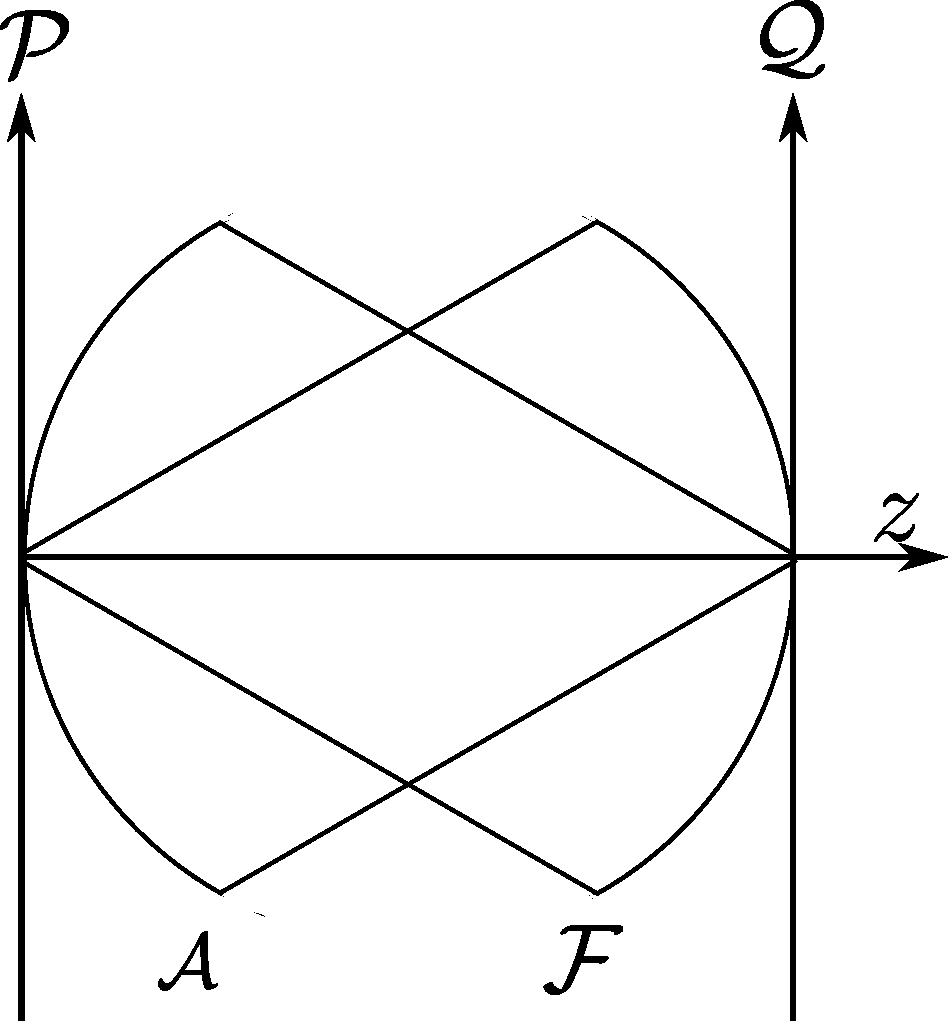
\includegraphics[width=0.5\linewidth]{Capitulo 1/Figuras/Cardinales}
	\caption{Esquema de las esferas cardinales confocales, con radios iguales a la distancia de propagación $z'$ del campo.}
	\label{fig:cardinals}
\end{figure}

Esto cobra más sentido una vez que analizamos el efecto de cada paso de propagación. Resulta claro que, sin imponer aproximaciones de campo lejano desde el inicio, al propagar el campo en $\mathcal{A}$ hacia $\mathcal{F}$ con la aproximación de Fresnel, obtendríamos
\begin{equation}
	U_{\mathcal{F}}(\vec{r}\,') = \dfrac{e^{ikz'}}{i\lambda z'} \exp\left( \frac{ik}{2z'} (x'^2 + y'^2) \right)  \int u_{\mathcal{A}}
	\exp\left( \frac{ik}{2z'} (x^2 + y^2) \right)
	\exp\left( -\frac{ik}{z'} (xx' + yy') \right)d\sigma ,
\end{equation}
donde podemos asociar $u_{\mathcal{A}}$, es decir, el campo sobre la esfera $\mathcal{A}$, con el campo sobre $\mathcal{P}$ multiplicado por su factor cuadrático correspondiente $u_{\mathcal{P}} = u_{\mathcal{A}} (\vec{r}) \exp{\left( \dfrac{ik}{2z'}(x^2+y^2) \right)}$, mientras que el término $\exp{\left( \frac{ik}{2z'} (x'^2 + y'^2) \right)}$ puede entenderse como el factor resultante de pasar el campo de la esfera $\mathcal{F}$ a la pantalla $\mathcal{Q}$, de modo que el campo sobre $\mathcal{F}$ correspondería a
\begin{equation}
	u_{\mathcal{Q}}(\vec{r}\,') = \dfrac{e^{ikz'}}{i\lambda z'} \int u_{\mathcal{P}}
	\exp\left( -\frac{ik}{z'} (xx' + yy') \right)d\sigma ,
\end{equation}
recuperando así una expresión de Fraunhofer para la difracción sobre $\mathcal{Q}$. Cabe señalar que debe verificarse si el estudio del campo propagado es válido dentro de un régimen paraxial, en el que el campo está confinado a la vecindad del eje óptico y por lo tanto la curvatura de la esfera cardinal no difiere mucho del plano (la pantalla). En los casos en que el factor de curvatura deja de ser despreciable, el régimen paraxial pierde validez y el problema debe abordarse desde un punto de vista metaxial.

Vale la pena detenerse aquí a contar, porque este es el lugar en que se cumple la promesa hecha al comienzo del capítulo. Diecisiete supuestos separan las ecuaciones de Maxwell de la integral de Fraunhofer \eqref{Fraunhofer}, y se agrupan en seis familias. Cinco fueron necesarios simplemente para reemplazar el campo electromagnético por una única cantidad escalar: se descartó la interacción magnética, se vació el medio de cargas y corrientes, se congeló la polarización primero en el tiempo y luego en el espacio, y se declaró transversal el campo. Un sexto redujo la luz policromática a una componente espectral a la vez. Cuatro más se gastaron en construir el aparato integral, exigiendo suavidad del campo, vaciando de fuentes la región de observación, reduciendo el emisor elemental a un punto y prohibiendo que llegara radiación alguna desde el infinito. Dos se gastaron en la pantalla, cuyo material fue idealizado hasta desaparecer y sobre la cual el campo fue luego prescrito a mano. Uno colocó al observador a muchas longitudes de onda de la abertura. Tres construyeron el régimen paraxial, truncando la expansión binomial, tratando la amplitud y la fase con distintos grados de precisión y enderezando a la unidad el factor de oblicuidad. El decimoséptimo y último empujó al observador hacia el campo lejano.

De este recuento se siguen dos lecciones. La primera es que la elegancia de \eqref{Fraunhofer}, una simple transformada de Fourier de la abertura, se compra en lugar de regalarse: cada uno de los diecisiete pasos ha estrechado la clase de experimentos que la fórmula puede describir, y cada uno de ellos puede violarse en un laboratorio. La teoría escalar falla cuando la abertura se vuelve comparable con la longitud de onda, cuando la apertura numérica es grande, cuando la pantalla es un buen conductor y la polarización de la iluminación resulta importar, o cuando la distancia de observación no es suficientemente grande para que el número de Fresnel sea pequeño; en cada uno de esos casos el culpable puede rastrearse hasta un elemento definido de la lista anterior. La segunda lección es la más notable, y es la razón por la que la teoría se enseña en absoluto: la fórmula funciona de todos modos, y funciona en un rango de situaciones mucho más amplio de lo que los supuestos tendrían derecho a garantizar. Entender cuál de los diecisiete está a punto de romperse es, en la práctica, todo el arte de aplicar la teoría de la difracción.


Estudiar la propagación del campo mediante la difracción de Fresnel es de gran importancia porque, como se discutirá más adelante, guarda una estrecha relación con lo que se conoce como la transformada fraccionaria de Fourier, una herramienta que surge naturalmente al encadenar pasos de propagación paraxial.

\section{La transformada fraccionaria de Fourier}\label{sec:FrFT}

	La sección anterior cerró con la observación de que la propagación de Fresnel guarda una estrecha relación con la transformada fraccionaria de Fourier. Esa observación es el tema de la presente sección, y merece un tratamiento cuidadoso por dos razones. La primera es que la transformada fraccionaria de Fourier no es una curiosidad formal sino el lenguaje natural en el que debería escribirse la propagación paraxial, en el mismo sentido en que la transformada de Fourier ordinaria es el lenguaje natural del campo lejano. La segunda es que el objeto en sí, una familia continua de operadores que interpola entre la identidad y la transformación de Fourier, tiene una historia larga e instructiva, en la que la misma idea fue redescubierta de manera independiente en el análisis puro, en la mecánica cuántica, en el procesamiento de señales y en la óptica, antes de que alguien se percatara de que las cuatro comunidades hablaban del mismo grupo uniparamétrico.

	Una palabra sobre notación antes de comenzar. En \eqref{Fresnel} la distancia de propagación aparecía como $z'$, la coordenada axial del punto de observación, quedando la abertura fija en el origen del eje. En la presente sección las dos superficies de referencia se tratan en pie de igualdad y ninguna de ellas está privilegiada, de modo que colocamos la superficie emisora en el origen y escribimos simplemente $z$ para la distancia a la receptora. La $z$ de esta sección es, por lo tanto, la $z'$ de \eqref{Fresnel}, y ninguna coordenada axial de la variable de integración aparece en ningún lugar de lo que sigue.


	\subsection{Contexto histórico del análisis de Fourier y de sus potencias fraccionarias}

		La historia comienza, como tantas historias de la física matemática, con una cuerda vibrante. En 1747 Jean le Rond d'Alembert escribió la ecuación de onda de una cuerda tensa y la resolvió superponiendo dos ondas viajeras \citep{dalembert1747recherches}, solución que Leonhard Euler generalizó de inmediato a formas iniciales arbitrarias \citep{euler1748vibration}. Seis años más tarde Daniel Bernoulli propuso algo que a sus contemporáneos les pareció físicamente obvio y matemáticamente escandaloso a la vez, a saber, que todo movimiento posible de la cuerda podía escribirse como una suma de los modos sinusoidales de vibración \citep{bernoulli1753reflexions}. Euler y d'Alembert rechazaron ambos la afirmación. Su objeción no era estética sino lógica, ya que una suma de senos es un objeto suave y periódico mientras que la forma inicial de una cuerda pulsada tiene un pico, y ningún matemático del siglo XVIII estaba dispuesto a aceptar que una suma infinita de funciones analíticas pudiera reproducir una curva con un quiebre. La disputa duró medio siglo y nunca fue zanjada por quienes la iniciaron.

		Quedó zanjada, en cierto sentido, por alguien que no intentaba zanjarla. En 1807 Joseph Fourier presentó al Institut de France una memoria sobre la propagación del calor en los sólidos en la que afirmaba, y usaba, precisamente la representación que Euler había rechazado. Los árbitros, entre ellos Lagrange, rechazaron la memoria. Lagrange en particular nunca aceptó la generalidad de la expansión trigonométrica, y Fourier tuvo que esperar hasta 1822 para publicar la versión madura de sus ideas como la \textit{Théorie Analytique de la Chaleur} \citep{fourier1822theorie}. Lo que Fourier había entendido, y sus árbitros no, es que la pregunta de si la serie converge a la función es una pregunta distinta de si la serie es útil, y que los coeficientes pueden calcularse mediante una integral sin importar la posición filosófica de cada quien sobre la convergencia. El paso de la serie sobre un intervalo finito a la integral sobre toda la recta, que es lo que hoy llamamos la transformación de Fourier, ya está presente en ese libro como un caso límite.

		La osadía de Fourier dejó una deuda que el siglo XIX pasó décadas pagando. Peter Gustav Lejeune Dirichlet dio en 1829 el primer teorema de convergencia genuino, mostrando que la serie de una función monótona a trozos con un número finito de discontinuidades converge al promedio de los límites laterales \citep{dirichlet1829convergence}. Bernhard Riemann, en su habilitación de 1854 publicada póstumamente en 1867, planteó la pregunta inversa de qué funciones admiten en absoluto una representación trigonométrica, y al hacerlo se vio obligado a inventar una teoría de la integración \citep{riemann1867darstellbarkeit}. Georg Cantor, estudiando la unicidad de las representaciones trigonométricas, fue llevado a clasificar los conjuntos excepcionales sobre los cuales dos series distintas pueden coincidir, y de esa clasificación creció la propia teoría de conjuntos \citep{cantor1872ausdehnung}. Henri Lebesgue construyó una nueva integral en parte para hacer que la teoría de las series trigonométricas se comportara \citep{lebesgue1903series}. No es exagerado decir que buena parte del análisis moderno existe porque Fourier escribió una fórmula que nadie podía justificar.

		La teoría alcanzó su forma definitiva en el siglo XX. Michel Plancherel demostró en 1910 la identidad que lleva su nombre, estableciendo que la transformación de Fourier es una isometría del espacio de funciones de cuadrado integrable sobre sí mismo \citep{plancherel1910contribution}. Este es, para nuestros propósitos, el hecho estructural más importante sobre la transformación, porque una isometría de un espacio de Hilbert sobre sí mismo es un operador unitario, y los operadores unitarios son exactamente los objetos que pueden elevarse a potencias continuas. Norbert Wiener \citeyearpar{wiener1933fourier} y Edward Titchmarsh \citeyearpar{titchmarsh1937introduction} consolidaron la teoría analítica en los dos tratados que definieron el tema durante una generación, y en 1965 James Cooley y John Tukey redescubrieron un algoritmo que redujo el costo numérico de la transformación discreta de una ley cuadrática a una logarítmica, y con ello llevó el análisis de Fourier del pizarrón a todos los instrumentos de laboratorio \citep{cooley1965algorithm}.

		La óptica entró en la historia por una puerta distinta. Ernst Abbe ya había entendido en 1873, tratando de explicar por qué sus microscopios no podían resolver detalles arbitrariamente finos, que el objetivo de un microscopio realiza una descomposición del objeto en frecuencias espaciales y que la abertura del instrumento trunca esa descomposición \citep{abbe1873beitrage}. La idea permaneció esencialmente cualitativa hasta que Pierre-Michel Duffieux publicó en 1946 el primer tratado sistemático sobre la integral de Fourier en óptica \citep{duffieux1946integrale}, antecesor directo del tratamiento moderno que se encuentra en Goodman \citeyearpar{goodman2005introduction}. Hacia mediados del siglo XX era un lugar común que el campo lejano de una abertura es la transformada de Fourier de la abertura, que es la afirmación que dedujimos en la sección sobre la aproximación de Fraunhofer.

		La idea de una potencia \textit{fraccionaria} de la transformación de Fourier tiene una genealogía separada y mucho menos lineal. Su semilla es una observación puramente analítica. Charles Hermite había introducido en 1864 los polinomios que llevan su nombre \citep{hermite1864nouveau}, y Ferdinand Gustav Mehler había hallado en 1866 la función generadora bilineal de esos polinomios \citep{mehler1866entwicklung}, fórmula que hará todo el trabajo por nosotros más adelante en esta sección. En 1929 Norbert Wiener publicó una breve nota en la que observaba que las funciones de Hermite son funciones propias de la transformación de Fourier con valores propios que son las cuatro raíces cuartas de la unidad \citep{wiener1929hermitian}. La observación es elemental una vez enunciada, pero es toda la idea, porque un operador cuyo espectro se conoce puede elevarse a cualquier potencia que se desee simplemente elevando los valores propios a esa potencia.

		Edward Uhler Condon dio ese paso explícitamente en 1937, en un artículo cuyo título dice exactamente lo que hace, a saber, sumergir la transformación de Fourier en un grupo continuo de transformaciones funcionales \citep{condon1937immersion}. Condon estaba interesado en la estructura teórico-grupal y en la conexión con el oscilador armónico cuántico, y ya notó que el generador de la familia continua es el hamiltoniano del oscilador. Dos años más tarde Hermann Kober, trabajando desde el punto de vista de las transformaciones integrales, construyó raíces de las transformaciones de Fourier y de Hankel y dio los núcleos correspondientes \citep{kober1939wurzeln}. Valentine Bargmann llegó a la misma familia en 1961 desde otra dirección distinta, a través de su espacio de Hilbert de funciones enteras, donde las potencias fraccionarias actúan como simples rotaciones de la variable compleja \citep{bargmann1961hilbert}. Nicolaas de Bruijn las recuperó una vez más en 1973 en su teoría de funciones generalizadas construida sobre la distribución de Wigner \citep{debruijn1973theory}. Cada uno de estos autores tuvo el objeto entre las manos y ninguno le dio un nombre que perdurara.

		El nombre y el tratamiento sistemático se deben a Victor Namias, quien en 1980 publicó el artículo que la comunidad óptica toma hoy como el origen del tema \citep{namias1980fractional}. La contribución de Namias no fue meramente terminológica. Definió la transformación de orden fraccionario de dos maneras equivalentes, como un operador diferencial obtenido al exponenciar el hamiltoniano del oscilador armónico y como un operador integral con núcleo explícito, mostró que las dos definiciones coinciden, y luego usó la herramienta resultante para resolver problemas concretos de mecánica cuántica que resultan incómodos en el lenguaje de Fourier ordinario. Es su derivación la que reproduciremos por completo en la siguiente subsección.

		El tratamiento de Namias fue, según sus propios estándares, el de un físico en ejercicio. La integral que escribió no converge absolutamente para toda función que uno quisiera transformar, la raíz cuadrada que aparece en la constante de normalización se escribe sin especificar qué rama se entiende, y la aditividad de los órdenes se verifica sobre la expansión en funciones propias en lugar de demostrarse en un dominio bien definido. Estas no son objeciones pedantes, porque una elección descuidada de rama hace que la ley de composición falle por un signo. Adam McBride y Fiona Kerr repararon todo esto en 1987 \citep{mcbride1987namias}, dando una definición que converge absolutamente en el espacio de Schwartz, fijando la rama de manera que la ley de composición se cumpla para todos los órdenes reales, y demostrando que la familia resultante es un genuino grupo continuo uniparamétrico. Kerr extendió poco después la construcción a espacios de funciones generalizadas \citep{kerr1988distributional} y al espacio de funciones de cuadrado integrable con aplicaciones a ecuaciones diferenciales \citep{kerr1988namias}.

		Mientras los analistas ordenaban la teoría, la comunidad óptica redescubrió el objeto experimentalmente. En 1993 David Mendlovic y Haldun Ozaktas publicaron un par de artículos mostrando que un medio de índice gradual de la longitud apropiada realiza una transformación fraccionaria de Fourier sobre el campo que lo atraviesa \citep{mendlovic1993fractional, ozaktas1993fractional}, y Adolf Lohmann mostró ese mismo año que el orden fraccionario no es otra cosa que un ángulo de rotación de la distribución de Wigner del campo, lo cual dio a toda la construcción un significado transparente en el espacio de fase y una implementación inmediata en óptica de volumen con dos lentes \citep{lohmann1993image}. Un año después Pierre Pellat-Finet demostró el resultado que más directamente nos concierne, a saber, que la difracción de Fresnel entre dos casquetes esféricos es exactamente una transformación fraccionaria de Fourier, con un orden fijado por la geometría \citep{pellatfinet1994fresnel}, resultado desarrollado extensamente junto con Georges Bonnet \citep{pellatfinet1994fractional} e incorporado más tarde a un tratado completo sobre óptica metaxial y fraccionaria de Fourier \citep{pellatfinet2009optique}. Paralelamente, Luís Almeida introdujo la transformación en el procesamiento de señales como una interpolación entre las representaciones temporal y frecuencial \citep{almeida1994fractional}, y todo el cuerpo de aplicaciones ópticas fue recopilado por Ozaktas, Zalevsky y Kutay \citeyearpar{ozaktas2001fractional}.

		Vale la pena detenerse en el hecho de que la literatura no usa una única noción de orden fraccionario, y un lector que se mueva entre artículos encontrará al menos cinco convenciones. La primera es la introducida por Namias, en la que el orden es un ángulo $\alpha$ medido en radianes, correspondiendo la transformación de Fourier ordinaria a $\alpha = \pi/2$ y la identidad a $\alpha = 0$. La segunda, estándar en el procesamiento de señales tras Ozaktas, Mendlovic y Lohmann, reemplaza el ángulo por un orden adimensional $a$ definido mediante $\alpha = a\pi/2$, de modo que la transformación ordinaria es la transformación de orden uno y el operador de paridad es la transformación de orden dos. La tercera es el orden óptico usado por Pellat-Finet, que de nuevo es un ángulo pero está ligado a un par de esferas de referencia en lugar de a una asignación abstracta de valores propios, y que por lo tanto depende de la geometría elegida para describir la propagación. La cuarta es el orden complejo, introducido por Chung-Chieh Shih \citeyearpar{shih1995optical} y realizado ópticamente por Luís Bernardo y Olívio Soares \citeyearpar{bernardo1996optical}, en la cual se permite que el parámetro abandone el eje real y la transformación adquiere una ponderación gaussiana además de su chirp. La quinta no es una convención sino una ambigüedad genuina, y merece énfasis. Puesto que la transformación de Fourier ordinaria satisface $\mathcal{F}^{4} = \mathcal{I}$, el problema de definir $\mathcal{F}^{a}$ es el problema de elegir de manera continua una raíz cuarta de la identidad, y esa elección no es única. Namias asigna a la función propia de índice $n$ el valor propio $e^{-in\alpha}$, que es la elección que hace del generador el hamiltoniano del oscilador armónico, pero Shih mostró que una asignación distinta y perfectamente consistente, basada en ponderar las cuatro potencias de $\mathcal{F}$, produce una familia inequivalente \citep{shih1995fractionalization}. Gianfranco Cariolaro y colaboradores clasificaron después todas las fraccionalizaciones admisibles en un único marco \citep{cariolaro1998unified}, y Çağatay Candan, Alper Kutay y Ozaktas resolvieron el problema discreto correspondiente \citep{candan2000discrete}. Cuando un artículo habla de \textit{la} transformada fraccionaria de Fourier sin mayor calificación, casi siempre se refiere a la familia de Namias, y es esa la que construiremos.

		Por último, cabe decir que la transformación fraccionaria de Fourier no es un objeto aislado sino el miembro no trivial más simple de una familia mucho más amplia. Marcos Moshinsky y Christiane Quesne introdujeron en 1971 las transformaciones canónicas lineales, las representaciones unitarias del grupo de transformaciones lineales del espacio de fase que preservan la forma simpléctica \citep{moshinsky1971linear}, y Kurt Bernardo Wolf desarrolló su teoría como transformaciones integrales \citep{wolf1979integral}. Stuart Collins había escrito en 1970 la integral de difracción de un sistema paraxial arbitrario en términos de la matriz de ese sistema \citep{collins1970lens}, que es la misma familia vista desde el lado de la ingeniería. En ese lenguaje, las transformaciones fraccionarias de Fourier son exactamente los elementos elípticos del grupo, es decir, las rotaciones del espacio de fase, mientras que la propagación libre sobre un plano y la acción de una lente delgada son elementos parabólicos y las magnificaciones son elementos hiperbólicos. La razón por la que la transformación fraccionaria de Fourier ocupa un lugar tan privilegiado en óptica es que, como demostraremos, una vez que el campo se refiere al par correcto de superficies esféricas, la propagación libre se convierte en una rotación pura.

	\subsection{La transformada fraccionaria de Fourier como operador diferencial e integral}

		A lo largo de esta subsección trabajamos en una sola variable transversal, ya que el caso bidimensional se sigue tomando el producto tensorial de dos transformaciones unidimensionales idénticas, y adoptamos la convención simétrica
		\begin{equation}\label{eq:FrFT:FT}
			\mathcal{F}[f](x) = \frac{1}{\sqrt{2\pi}}\int_{-\infty}^{\infty} f(y)\,e^{-ixy}\,\mathrm{d}y,
		\end{equation}
		que es la convención que hace a $\mathcal{F}$ unitaria sobre $L^2(\mathbb{R})$ por el teorema de Plancherel \citeyearpar{plancherel1910contribution}, y que concuerda con el signo del núcleo que apareció en la integral de Fraunhofer \eqref{Fraunhofer}. Aplicando \eqref{eq:FrFT:FT} dos veces se obtiene el operador de paridad, y cuatro veces la identidad,
		\begin{equation}\label{eq:FrFT:Powers}
			\mathcal{F}^{2} = \mathcal{P}, \qquad \mathcal{P}f(x) = f(-x), \qquad \mathcal{F}^{4} = \mathcal{I},
		\end{equation}
		de modo que las potencias enteras de $\mathcal{F}$ forman un grupo cíclico de orden cuatro. Todo el contenido de esta subsección es la construcción de un grupo continuo en el cual ese grupo cíclico de cuatro elementos se aloja como subgrupo.

		Antes de comenzar, es necesario fijar un punto de vocabulario, porque las dos palabras involucradas se confunden rutinariamente y la distinción es esencial para todo lo que sigue.

		\begin{myDef}
			\textit{(Transformación y transformada)} Una \textit{transformación} es un operador, es decir, una aplicación $\mathcal{F}_{\alpha} : \mathcal{H} \to \mathcal{H}$ de un espacio de funciones en sí mismo. Una \textit{transformada} es la imagen de un elemento particular bajo esa aplicación, es decir, la función $\mathcal{F}_{\alpha}f$ obtenida al aplicar la transformación a una $f$ dada.
		\end{myDef}

		La distinción no es pedante. Todo lo que hace valiosa a la construcción fraccionaria de Fourier es un enunciado sobre \textit{transformaciones} y no sobre transformadas: la familia $\{\mathcal{F}_{\alpha}\}_{\alpha\in\mathbb{R}}$ es un grupo uniparamétrico, su ley de composición es $\mathcal{F}_{\alpha}\mathcal{F}_{\beta} = \mathcal{F}_{\alpha+\beta}$, su generador es el hamiltoniano del oscilador armónico, y sus elementos son unitarios. Ninguna de estas frases puede siquiera formularse al nivel de una única transformada, porque una transformada es simplemente una función y no lleva estructura de grupo alguna. En la aplicación óptica de la subsección anterior, el punto se vuelve físico en lugar de lingüístico: es la propagación del campo a lo largo de una distancia lo que es una transformación, mientras que el campo observado sobre la superficie receptora es una transformada, y la razón por la cual la propagación se compone de manera tan simple es una propiedad de los operadores, no de ningún campo en particular.

		\subsubsection{Las funciones propias de la transformación de Fourier}

			La construcción descansa sobre un único hecho, observado por Wiener en 1929 \citep{wiener1929hermitian}, a saber, que la transformación de Fourier posee un conjunto ortonormal completo de funciones propias construidas a partir de los polinomios de Hermite \citep{hermite1864nouveau}. Deduzcámoslo, ya que cada paso posterior depende del valor preciso de los valores propios. Recordemos la función generadora de los polinomios de Hermite,
			\begin{equation}\label{eq:FrFT:HermiteGen}
				e^{2xt-t^{2}} = \sum_{n=0}^{\infty}\frac{H_{n}(x)}{n!}t^{n},
			\end{equation}
			y definamos la función generadora de las funciones de Hermite multiplicando \eqref{eq:FrFT:HermiteGen} por la gaussiana $e^{-x^{2}/2}$,
			\begin{equation}\label{eq:FrFT:GDef}
				G(x,t) = e^{-x^{2}/2}\,e^{2xt-t^{2}} = e^{-x^{2}/2}\sum_{n=0}^{\infty}\frac{H_{n}(x)}{n!}t^{n}.
			\end{equation}
			Transformamos ahora \eqref{eq:FrFT:GDef} respecto a $x$. Escribiendo el exponente completo del integrando de \eqref{eq:FrFT:FT},
			\begin{align*}
				& -\frac{x^{2}}{2} + 2xt - t^{2} - i\xi x = -\frac{x^{2}}{2} + x\left(2t-i\xi\right) - t^{2} = \\
				& -\frac{1}{2}\left[x^{2} - 2x\left(2t-i\xi\right) + {\color{blue}\left(2t-i\xi\right)^{2}}\right] + {\color{blue}\frac{\left(2t-i\xi\right)^{2}}{2}} - t^{2},
			\end{align*}
			donde los dos términos en azul se han sumado y restado, lo cual es lícito porque su suma es cero, y lo cual convierte el primer corchete en un cuadrado perfecto,
			\begin{equation*}
				= -\frac{1}{2}\left[x - \left(2t-i\xi\right)\right]^{2} + \frac{\left(2t-i\xi\right)^{2}}{2} - t^{2}.
			\end{equation*}
			La integral restante es la gaussiana $\int_{-\infty}^{\infty}e^{-\frac{1}{2}(x-a)^{2}}\mathrm{d}x = \sqrt{2\pi}$, válida para $a$ compleja mediante una traslación del contorno de integración, de modo que el factor $1/\sqrt{2\pi}$ de \eqref{eq:FrFT:FT} se cancela exactamente y
			\begin{equation}\label{eq:FrFT:GTransformed}
				\mathcal{F}\left[G(\cdot,t)\right](\xi) = \exp\left[\frac{\left(2t-i\xi\right)^{2}}{2} - t^{2}\right].
			\end{equation}
			Resta reconocer el lado derecho. Expandiendo el cuadrado,
			\begin{align*}
				& \frac{4t^{2} - 4it\xi - \xi^{2}}{2} - t^{2} = 2t^{2} - 2it\xi - \frac{\xi^{2}}{2} - t^{2} = -\frac{\xi^{2}}{2} - 2i\xi t + t^{2} = \\
				& -\frac{\xi^{2}}{2} + 2\xi\left(-it\right) - \left(-it\right)^{2},
			\end{align*}
			puesto que $-(-it)^{2} = +t^{2}$, y comparando con la definición \eqref{eq:FrFT:GDef} concluimos que
			\begin{equation}\label{eq:FrFT:GSelf}
				\mathcal{F}\left[G(\cdot,t)\right](\xi) = G(\xi,-it).
			\end{equation}
			\textit{La función generadora se aplica sobre sí misma con el parámetro rotado un cuarto de vuelta en el plano complejo.} Expandiendo ambos lados de \eqref{eq:FrFT:GSelf} en potencias de $t$ mediante \eqref{eq:FrFT:GDef},
			\begin{equation*}
				\sum_{n=0}^{\infty}\frac{t^{n}}{n!}\,\mathcal{F}\!\left[H_{n}\,e^{-x^{2}/2}\right](\xi) = \sum_{n=0}^{\infty}\frac{\left(-it\right)^{n}}{n!}H_{n}(\xi)e^{-\xi^{2}/2},
			\end{equation*}
			e identificando los coeficientes de $t^{n}$, lo cual es lícito porque ambas series convergen para todo $t$ en una vecindad del origen, obtenemos el resultado buscado. Introduciendo las funciones de Hermite normalizadas
			\begin{equation}\label{eq:FrFT:HermiteFunctions}
				\psi_{n}(x) = \left(2^{n}n!\sqrt{\pi}\right)^{-1/2}H_{n}(x)\,e^{-x^{2}/2}, \qquad \int_{-\infty}^{\infty}\psi_{n}(x)\psi_{m}(x)\,\mathrm{d}x = \delta_{nm},
			\end{equation}
			que forman una base ortonormal completa de $L^{2}(\mathbb{R})$, la relación de valores propios se lee
			\begin{equation}\label{eq:FrFT:Eigen}
				\mathcal{F}\left[\psi_{n}\right] = \left(-i\right)^{n}\psi_{n} = e^{-in\pi/2}\,\psi_{n}.
			\end{equation}

			La ecuación \eqref{eq:FrFT:Eigen} contiene toda la idea. Los valores propios de la transformación de Fourier son $e^{-in\pi/2}$, y el número $\pi/2$ aparece allí no por ninguna propiedad profunda de la exponencial, sino simplemente porque $\mathcal{F}$ es la raíz cuarta de la identidad. Nada nos impide reemplazar $\pi/2$ por un ángulo arbitrario.

		\subsubsection{La definición de Namias y el operador diferencial}

			Siguiendo a Namias \citeyearpar{namias1980fractional}, definimos la transformación fraccionaria de Fourier de orden $\alpha$ prescribiendo su acción sobre la base \eqref{eq:FrFT:HermiteFunctions},
			\begin{equation}\label{eq:FrFT:SpectralDef}
				\mathcal{F}_{\alpha}\left[\psi_{n}\right] = e^{-in\alpha}\,\psi_{n},
			\end{equation}
			y extendiéndola a una $f\in L^{2}(\mathbb{R})$ arbitraria por linealidad y continuidad. Escribiendo la expansión de $f$ en la base,
			\begin{equation}\label{eq:FrFT:Expansion}
				f(x) = \sum_{n=0}^{\infty}c_{n}\psi_{n}(x), \qquad c_{n} = \int_{-\infty}^{\infty}f(y)\psi_{n}(y)\,\mathrm{d}y,
			\end{equation}
			la transformada de orden $\alpha$ es por definición
			\begin{equation}\label{eq:FrFT:SpectralTransform}
				F_{\alpha}(x) \equiv \mathcal{F}_{\alpha}\left[f\right](x) = \sum_{n=0}^{\infty}c_{n}e^{-in\alpha}\psi_{n}(x).
			\end{equation}
			La definición es manifiestamente consistente, ya que $\alpha = 0$ da $F_{0} = f$ por completitud, $\alpha = \pi/2$ reproduce \eqref{eq:FrFT:Eigen}, $\alpha = \pi$ da $\sum c_{n}(-1)^{n}\psi_{n}$, que es el operador de paridad porque $\psi_{n}$ tiene la paridad de $n$, y $\alpha = 2\pi$ devuelve la identidad. La familia es por lo tanto $2\pi$-periódica en $\alpha$ y unitaria, ya que multiplica los coeficientes de una expansión ortonormal por números unimodulares.

			La primera observación de Namias es que \eqref{eq:FrFT:SpectralTransform} puede liberarse de la base y escribirse como un operador diferencial. Derivando \eqref{eq:FrFT:SpectralTransform} respecto al orden,
			\begin{equation}\label{eq:FrFT:dFdalpha}
				\frac{\partial F_{\alpha}}{\partial \alpha}(x) = -i\sum_{n=0}^{\infty}n\,c_{n}e^{-in\alpha}\psi_{n}(x),
			\end{equation}
			nos queda el índice $n$ dentro de la suma, lo cual es inconveniente porque $n$ no es un operador que actúe sobre $x$. El remedio es la ecuación diferencial de las funciones de Hermite. Sustituyendo \eqref{eq:FrFT:HermiteFunctions} en la ecuación de Hermite $H_{n}'' - 2xH_{n}' + 2nH_{n} = 0$ se obtiene, tras el cálculo elemental de las dos derivadas del factor gaussiano,
			\begin{equation}\label{eq:FrFT:HermiteODE}
				\psi_{n}''(x) + \left(2n+1-x^{2}\right)\psi_{n}(x) = 0,
			\end{equation}
			que es precisamente la ecuación de Schrödinger estacionaria del oscilador armónico cuántico en unidades naturales. Resolviendo \eqref{eq:FrFT:HermiteODE} para el índice,
			\begin{equation}\label{eq:FrFT:nPsi}
				n\,\psi_{n}(x) = \frac{1}{2}\left[x^{2}\psi_{n}(x) - \psi_{n}''(x) - \psi_{n}(x)\right],
			\end{equation}
			e insertando \eqref{eq:FrFT:nPsi} en \eqref{eq:FrFT:dFdalpha},
			\begin{align*}
				& \frac{\partial F_{\alpha}}{\partial \alpha}(x) = -\frac{i}{2}\sum_{n=0}^{\infty}c_{n}e^{-in\alpha}\left[x^{2}\psi_{n}(x) - \psi_{n}''(x) - \psi_{n}(x)\right] = \\
				& -\frac{i}{2}\left[x^{2}\sum_{n}c_{n}e^{-in\alpha}\psi_{n}(x) - \frac{\partial^{2}}{\partial x^{2}}\sum_{n}c_{n}e^{-in\alpha}\psi_{n}(x) - \sum_{n}c_{n}e^{-in\alpha}\psi_{n}(x)\right],
			\end{align*}
			donde el índice $n$ ha desaparecido por completo y cada una de las tres sumas es de nuevo $F_{\alpha}$ por \eqref{eq:FrFT:SpectralTransform}. Llegamos así a la formulación diferencial de la transformación fraccionaria de Fourier,
			\begin{equation}\label{eq:FrFT:PDE}
				i\,\frac{\partial F_{\alpha}}{\partial \alpha} = \frac{1}{2}\left[-\frac{\partial^{2}}{\partial x^{2}} + x^{2} - 1\right]F_{\alpha}, \qquad F_{\alpha}\big|_{\alpha=0} = f.
			\end{equation}

			\textbf{\textit{La ecuación \eqref{eq:FrFT:PDE} es la definición de Namias de la transformación fraccionaria de Fourier como operador diferencial.}} Vale la pena leerla dos veces. Afirma que la transformada de orden $\alpha$ de una función dada se obtiene dejando que esa función evolucione, según la ecuación de Schrödinger del oscilador armónico, durante un \textit{tiempo} igual a $\alpha$, siendo la constante $-1$ la que simplemente elimina la energía de punto cero para que el estado fundamental no acumule fase. En lenguaje de operadores, introduciendo el hamiltoniano del oscilador
			\begin{equation}\label{eq:FrFT:Hamiltonian}
				\hat{H} = \frac{1}{2}\left(-\frac{\partial^{2}}{\partial x^{2}} + x^{2}\right), \qquad \hat{H}\psi_{n} = \left(n+\frac{1}{2}\right)\psi_{n},
			\end{equation}
			la solución de \eqref{eq:FrFT:PDE} se escribe de inmediato como la exponencial del generador,
			\begin{equation}\label{eq:FrFT:Exponential}
				\mathcal{F}_{\alpha} = \exp\left[-i\alpha\left(\hat{H}-\frac{1}{2}\right)\right] = \exp\left[\frac{i\alpha}{2}\left(\frac{\partial^{2}}{\partial x^{2}} - x^{2} + 1\right)\right],
			\end{equation}
			que reproduce \eqref{eq:FrFT:SpectralDef} de inmediato, ya que $\exp[-i\alpha(\hat{H}-\tfrac{1}{2})]\psi_{n} = e^{-i\alpha n}\psi_{n}$. Esta identificación es la razón por la cual la transformación fraccionaria de Fourier aparece dondequiera que aparece un oscilador armónico, y explica retrospectivamente por qué Condon ya se había encontrado con la misma familia en 1937 al estudiar grupos continuos de transformaciones funcionales \citep{condon1937immersion}.

			De \eqref{eq:FrFT:Exponential} se siguen de inmediato dos consecuencias estructurales. Primero, puesto que las exponenciales de un único generador conmutan y suman sus argumentos,
			\begin{equation}\label{eq:FrFT:GroupExp}
				\mathcal{F}_{\alpha}\mathcal{F}_{\beta} = \mathcal{F}_{\alpha+\beta}, \qquad \mathcal{F}_{\alpha}^{-1} = \mathcal{F}_{-\alpha},
			\end{equation}
			de modo que las transformaciones forman un grupo uniparamétrico conmutativo. Segundo, puesto que $\hat{H}$ es autoadjunto, $\mathcal{F}_{\alpha}$ es unitaria, y el teorema de Plancherel se extiende a todo orden,
			\begin{equation}\label{eq:FrFT:Plancherel}
				\int_{-\infty}^{\infty}\left|\mathcal{F}_{\alpha}[f](x)\right|^{2}\mathrm{d}x = \int_{-\infty}^{\infty}\left|f(x)\right|^{2}\mathrm{d}x,
			\end{equation}
			lo cual, en la lectura óptica de la siguiente subsección, no es otra cosa que la conservación de la energía transportada por el campo.

		\subsubsection{La forma integral de la transformación}

			La forma diferencial \eqref{eq:FrFT:PDE} es compacta y conceptualmente transparente, pero para el cálculo se quiere un núcleo. Puesto que la transformación es lineal y acotada, debe ser representable como
			\begin{equation}\label{eq:FrFT:KernelDef}
				\mathcal{F}_{\alpha}[f](x) = \int_{-\infty}^{\infty}K_{\alpha}(x,y)f(y)\,\mathrm{d}y,
			\end{equation}
			e insertando la expansión \eqref{eq:FrFT:Expansion} en \eqref{eq:FrFT:SpectralTransform} e intercambiando la suma con la integral, el núcleo se lee como la suma espectral bilineal
			\begin{equation}\label{eq:FrFT:KernelSum}
				K_{\alpha}(x,y) = \sum_{n=0}^{\infty}e^{-in\alpha}\psi_{n}(x)\psi_{n}(y).
			\end{equation}
			Sustituyendo las funciones de Hermite explícitas \eqref{eq:FrFT:HermiteFunctions},
			\begin{equation}\label{eq:FrFT:KernelHermite}
				K_{\alpha}(x,y) = \frac{e^{-\left(x^{2}+y^{2}\right)/2}}{\sqrt{\pi}}\sum_{n=0}^{\infty}\frac{H_{n}(x)H_{n}(y)}{2^{n}n!}\,e^{-in\alpha},
			\end{equation}
			nos queda una función generadora bilineal de polinomios de Hermite, que es exactamente el objeto que Mehler calculó en 1866 \citep{mehler1866entwicklung},
			\begin{equation}\label{eq:FrFT:Mehler}
				\sum_{n=0}^{\infty}\frac{H_{n}(x)H_{n}(y)}{2^{n}n!}\,t^{n} = \frac{1}{\sqrt{1-t^{2}}}\exp\left[\frac{2xyt - \left(x^{2}+y^{2}\right)t^{2}}{1-t^{2}}\right], \qquad |t|<1.
			\end{equation}
			Debemos hacer $t = e^{-i\alpha}$, que se encuentra en el borde del disco de convergencia, de modo que \eqref{eq:FrFT:Mehler} debe entenderse como el límite $t\to e^{-i\alpha}$ tomado radialmente desde el interior del disco, límite que existe en el sentido de las distribuciones y que es lícito para todo $\alpha$ que no sea un múltiplo entero de $\pi$. Llevemos a cabo ahora el álgebra paso a paso. El denominador se factoriza como
			\begin{equation}\label{eq:FrFT:Denominator}
				1 - e^{-2i\alpha} = e^{-i\alpha}\left(e^{i\alpha} - e^{-i\alpha}\right) = e^{-i\alpha}\,2i\sin\alpha,
			\end{equation}
			de modo que el término cruzado del exponente de \eqref{eq:FrFT:Mehler} se convierte en
			\begin{equation}\label{eq:FrFT:CrossTerm}
				\frac{2xy\,{\color{red}e^{-i\alpha}}}{{\color{red}e^{-i\alpha}}\,2i\sin\alpha} = \frac{xy}{i\sin\alpha} = -\frac{i\,xy}{\sin\alpha} = -ixy\csc\alpha,
			\end{equation}
			donde las dos exponenciales en rojo se cancelan. Para el término cuadrático no debemos olvidar el prefactor gaussiano de \eqref{eq:FrFT:KernelHermite}, así que reunimos ambas contribuciones,
			\begin{align*}
				& -\frac{x^{2}+y^{2}}{2} - \frac{\left(x^{2}+y^{2}\right)e^{-2i\alpha}}{e^{-i\alpha}\,2i\sin\alpha} = -\frac{x^{2}+y^{2}}{2} - \frac{\left(x^{2}+y^{2}\right)e^{-i\alpha}}{2i\sin\alpha} = \\
				& -\frac{x^{2}+y^{2}}{2}\left[1 + \frac{e^{-i\alpha}}{i\sin\alpha}\right] = -\frac{x^{2}+y^{2}}{2}\cdot\frac{i\sin\alpha + e^{-i\alpha}}{i\sin\alpha},
			\end{align*}
			y el numerador de esta última fracción colapsa hermosamente,
			\begin{equation}\label{eq:FrFT:Collapse}
				i\sin\alpha + e^{-i\alpha} = {\color{red}i\sin\alpha} + \cos\alpha - {\color{red}i\sin\alpha} = \cos\alpha,
			\end{equation}
			de modo que, usando $-1/i = i$,
			\begin{equation}\label{eq:FrFT:QuadTerm}
				-\frac{x^{2}+y^{2}}{2}\cdot\frac{\cos\alpha}{i\sin\alpha} = \frac{i}{2}\left(x^{2}+y^{2}\right)\cot\alpha.
			\end{equation}
			Queda la constante de normalización. Usando de nuevo \eqref{eq:FrFT:Denominator},
			\begin{equation}\label{eq:FrFT:Constant}
				\frac{1}{\sqrt{\pi}}\cdot\frac{1}{\sqrt{1-e^{-2i\alpha}}} = \frac{1}{\sqrt{\pi}}\cdot\frac{e^{i\alpha/2}}{\sqrt{2i\sin\alpha}} = \frac{e^{i\left(\frac{\alpha}{2}-\frac{\pi}{4}\right)}}{\sqrt{2\pi\sin\alpha}},
			\end{equation}
			ya que $1/\sqrt{i} = e^{-i\pi/4}$. Esta constante se escribe más a menudo en la forma compacta que usó Namias, y las dos concuerdan porque
			\begin{equation}\label{eq:FrFT:ConstantEquiv}
				1 - i\cot\alpha = \frac{\sin\alpha - i\cos\alpha}{\sin\alpha} = \frac{-i\left(\cos\alpha + i\sin\alpha\right)}{\sin\alpha} = \frac{e^{-i\pi/2}e^{i\alpha}}{\sin\alpha},
			\end{equation}
			cuya raíz cuadrada dividida por $\sqrt{2\pi}$ es precisamente \eqref{eq:FrFT:Constant}. Reuniendo \eqref{eq:FrFT:CrossTerm}, \eqref{eq:FrFT:QuadTerm} y \eqref{eq:FrFT:Constant} obtenemos la forma integral de la transformación,
			\begin{equation}\label{eq:FrFT:Kernel}
				\boxed{\;\mathcal{F}_{\alpha}[f](x) = \sqrt{\frac{1-i\cot\alpha}{2\pi}}\int_{-\infty}^{\infty}\exp\left\{\frac{i}{2}\left(x^{2}+y^{2}\right)\cot\alpha - i\,xy\csc\alpha\right\}f(y)\,\mathrm{d}y.\;}
			\end{equation}

			Verifiquemos que \eqref{eq:FrFT:Kernel} hace lo que debe. Para $\alpha = \pi/2$ tenemos $\cot\alpha = 0$ y $\csc\alpha = 1$, de modo que la constante se reduce a $1/\sqrt{2\pi}$ y el núcleo a $e^{-ixy}$, recuperando exactamente la transformación ordinaria \eqref{eq:FrFT:FT}. Para $\alpha\to 0$ el coeficiente $\cot\alpha$ diverge y el núcleo oscila infinitamente rápido en todas partes salvo sobre la diagonal, donde el exponente $\frac{i}{2}(x-y)^{2}\cot\alpha$ se anula, y un argumento estándar de fase estacionaria muestra que $K_{\alpha}\to\delta(x-y)$, que es la identidad. Para $\alpha\to\pi$ el mismo argumento aplicado a $\frac{i}{2}(x+y)^{2}\cot\alpha$ da $K_{\pi}(x,y) = \delta(x+y)$, el operador de paridad. Los tres órdenes degenerados $\alpha = 0,\pi,2\pi$, en los cuales la fórmula cerrada \eqref{eq:FrFT:Kernel} carece de sentido porque $\csc\alpha$ diverge, están por lo tanto perfectamente bien definidos en la forma espectral \eqref{eq:FrFT:KernelSum}, discrepancia sobre la que habrá que volver.

		\subsubsection{La transformación inversa y la ley de índices}

			La inversa se obtiene sin ningún cálculo nuevo, porque \eqref{eq:FrFT:KernelSum} hace transparente la composición de dos transformaciones. Consideremos el núcleo del producto $\mathcal{F}_{\alpha}\mathcal{F}_{\beta}$,
			\begin{align*}
				& \int_{-\infty}^{\infty}K_{\alpha}(x,s)K_{\beta}(s,y)\,\mathrm{d}s = \int_{-\infty}^{\infty}\left[\sum_{n}e^{-in\alpha}\psi_{n}(x)\psi_{n}(s)\right]\left[\sum_{m}e^{-im\beta}\psi_{m}(s)\psi_{m}(y)\right]\mathrm{d}s = \\
				& \sum_{n}\sum_{m}e^{-in\alpha}e^{-im\beta}\psi_{n}(x)\psi_{m}(y)\underbrace{\int_{-\infty}^{\infty}\psi_{n}(s)\psi_{m}(s)\,\mathrm{d}s}_{\delta_{nm}} = \sum_{n}e^{-in\left(\alpha+\beta\right)}\psi_{n}(x)\psi_{n}(y),
			\end{align*}
			donde la ortonormalidad \eqref{eq:FrFT:HermiteFunctions} ha colapsado la doble suma en una sola, y la última expresión es por definición $K_{\alpha+\beta}(x,y)$. Hemos demostrado así la \textit{ley de índices}
			\begin{equation}\label{eq:FrFT:IndexLaw}
				\mathcal{F}_{\alpha}\mathcal{F}_{\beta} = \mathcal{F}_{\alpha+\beta},
			\end{equation}
			que es la propiedad que justifica llamar orden a $\alpha$, ya que los órdenes se suman bajo composición exactamente como lo hacen los exponentes. Haciendo $\beta = -\alpha$ y usando la completitud,
			\begin{equation}\label{eq:FrFT:Completeness}
				K_{0}(x,y) = \sum_{n=0}^{\infty}\psi_{n}(x)\psi_{n}(y) = \delta(x-y),
			\end{equation}
			concluimos que $\mathcal{F}_{\alpha}\mathcal{F}_{-\alpha} = \mathcal{I}$, es decir,
			\begin{equation}\label{eq:FrFT:Inverse}
				\mathcal{F}_{\alpha}^{-1} = \mathcal{F}_{-\alpha},
			\end{equation}
			de modo que la transformación inversa es la transformación de orden opuesto. Explícitamente, reemplazando $\alpha$ por $-\alpha$ en \eqref{eq:FrFT:Kernel} y usando $\cot(-\alpha) = -\cot\alpha$ y $\csc(-\alpha) = -\csc\alpha$,
			\begin{equation}\label{eq:FrFT:InverseKernel}
				f(y) = \sqrt{\frac{1+i\cot\alpha}{2\pi}}\int_{-\infty}^{\infty}\exp\left\{-\frac{i}{2}\left(x^{2}+y^{2}\right)\cot\alpha + i\,xy\csc\alpha\right\}F_{\alpha}(x)\,\mathrm{d}x,
			\end{equation}
			y comparando \eqref{eq:FrFT:InverseKernel} con \eqref{eq:FrFT:Kernel} vemos que $K_{-\alpha}(y,x) = \overline{K_{\alpha}(x,y)}$, que es precisamente el enunciado de que $\mathcal{F}_{\alpha}$ es unitaria, en concordancia con \eqref{eq:FrFT:Plancherel}.

		\subsubsection{La regularización de McBride y Kerr}

			La derivación que acabamos de llevar a cabo es la derivación de Namias, y como pieza de física está completa. Como pieza de análisis tiene tres huecos, todos ellos identificados y reparados por Adam McBride y Fiona Kerr en 1987 \citep{mcbride1987namias}. Puesto que la literatura óptica moderna usa su versión sin siempre decirlo, vale la pena enunciar qué cambiaron.

			El primer hueco es la \textit{rama de la raíz cuadrada}. La constante en \eqref{eq:FrFT:Kernel} se escribe como $\sqrt{1-i\cot\alpha}$, y una raíz cuadrada de un número complejo está definida solo salvo un signo. La suma espectral \eqref{eq:FrFT:KernelSum} no tiene tal ambigüedad, así que el signo debe fijarse haciendo coincidir ambas, y la determinación correcta es la ya contenida en \eqref{eq:FrFT:Constant}, que escrita sin ambigüedad se lee
			\begin{equation}\label{eq:FrFT:Branch}
				C_{\alpha} = \frac{\exp\left[i\left(\dfrac{\alpha}{2} - \dfrac{\pi}{4}\,\mathrm{sgn}\left(\sin\alpha\right)\right)\right]}{\sqrt{2\pi\left|\sin\alpha\right|}}.
			\end{equation}

			El factor discreto $\mathrm{sgn}(\sin\alpha)$ no es cosmético. Si se elige ingenuamente la rama principal y se componen dos transformaciones cuyos órdenes suman más de $\pi$, la ley de índices \eqref{eq:FrFT:IndexLaw} falla por un factor $-1$. Esta es la manifestación elemental de un fenómeno bien conocido, a saber, que el grupo de transformaciones no está representado fielmente por los núcleos sino por un recubrimiento doble de ellos, siendo el signo adicional lo que se llama el índice de Maslov en la teoría de las transformaciones canónicas \citep{moshinsky1971linear, wolf1979integral}.

			El segundo hueco es el \textbf{dominio y la convergencia de la integral}. Para una $f\in L^{2}(\mathbb{R})$ general, la integral en \eqref{eq:FrFT:Kernel} no converge absolutamente, porque el módulo del núcleo es constante en $y$ y el integrando por lo tanto no decae más rápido que la propia $f$. McBride y Kerr definen la transformación primero sobre el espacio de Schwartz $\mathcal{S}$ de funciones de decrecimiento rápido, donde la convergencia absoluta está garantizada, demuestran que $\mathcal{F}_{\alpha}$ aplica $\mathcal{S}$ sobre $\mathcal{S}$ de manera homeomorfa, y solo entonces la extienden por dualidad al espacio $\mathcal{S}'$ de las distribuciones temperadas. Su artificio técnico para ampliar el dominio consiste en intercambiar una potencia de decrecimiento en la variable de integración por una derivada en la variable de observación, reemplazando \eqref{eq:FrFT:Kernel} por una expresión de la forma
			\begin{equation}\label{eq:FrFT:MKForm}
				\mathcal{F}_{\alpha}[f](x) = C_{\alpha}\,e^{\frac{i}{2}x^{2}\cot\alpha}\,\frac{\mathrm{d}}{\mathrm{d}x}\int_{-\infty}^{\infty}\frac{e^{-ixy\csc\alpha}}{-i\,y\csc\alpha}\,e^{\frac{i}{2}y^{2}\cot\alpha}f(y)\,\mathrm{d}y,
			\end{equation}
			en la cual el factor adicional $1/y$ hace que la integral converja absolutamente para funciones que no son en sí mismas integrables, mientras que la derivada tomada fuera de la integral restaura el núcleo original. Una vez que se demuestra que el operador resultante es continuo sobre $\mathcal{S}$, la extensión a $\mathcal{S}'$ es automática, y los órdenes degenerados $\alpha = n\pi$ adquieren su significado correcto como los núcleos distribucionales $\delta(x\mp y)$ en lugar de aparecer como integrales divergentes.

			El tercer hueco es que Namias verifica la ley de índices \eqref{eq:FrFT:IndexLaw} sobre la expansión en funciones propias, que es una manipulación formal de una suma doblemente infinita. McBride y Kerr la demuestran como teorema para todo $\alpha$ y $\beta$ reales sobre un dominio establecido, y con ello demuestran que
			\begin{equation}\label{eq:FrFT:Group}
				\left\{\mathcal{F}_{\alpha}\right\}_{\alpha\in\mathbb{R}}, \qquad \mathcal{F}_{0} = \mathcal{I}, \qquad \mathcal{F}_{\alpha+2\pi} = \mathcal{F}_{\alpha},
			\end{equation}
			es un genuino grupo continuo uniparamétrico de homeomorfismos de $\mathcal{S}$, unitario sobre $L^{2}(\mathbb{R})$. Kerr desarrolló después en detalle la teoría distribucional \citep{kerr1988distributional} y la teoría en $L^{2}$ junto con aplicaciones a ecuaciones diferenciales \citep{kerr1988namias}. Solo con estas tres reparaciones, y únicamente con ellas, se tiene derecho a manipular $\mathcal{F}_{\alpha}$ como un objeto algebraico, que es lo que haremos libremente en la siguiente subsección.

		\subsubsection{Por qué la construcción es útil}

			Las dos caras de la transformación, la diferencial y la integral, son útiles en circunstancias distintas, y vale la pena separarlas.

			La \textit{forma diferencial} \eqref{eq:FrFT:PDE} es útil siempre que el oscilador armónico se esconde en el problema, lo cual sucede con mucha más frecuencia de la que cabría esperar. La motivación del propio Namias fue cuántica \citep{namias1980fractional}: puesto que $\mathcal{F}_{\alpha}$ es el operador de evolución del oscilador, la transformada fraccionaria de un paquete de onda inicial \textit{es} el paquete de onda en un instante posterior, de modo que los problemas de evolución temporal se convierten en problemas de elegir un orden, y el bien conocido renacimiento de un paquete de onda tras un período completo es simplemente la periodicidad $2\pi$ de \eqref{eq:FrFT:Group}. De manera más general, puesto que $\mathcal{F}_{\alpha}$ intercambia los operadores $x$ y $-i\partial_{x}$ mediante una rotación de ángulo $\alpha$, una ecuación diferencial con coeficientes polinómicos con frecuencia puede rotarse hasta una más simple, que es la técnica que Kerr sistematizó \citep{kerr1988namias}. El mismo generador gobierna el problema de Landau, la ecuación de onda paraxial en un medio de índice cuadrático, y la dinámica linealizada de cualquier sistema cerca de un equilibrio estable, de modo que la forma diferencial se transfiere de inmediato a todos ellos.

			La \textit{forma integral} \eqref{eq:FrFT:Kernel} es útil siempre que se necesita calcular en lugar de razonar. En el procesamiento de señales proporciona un continuo de representaciones que interpolan entre el dominio temporal y el frecuencial, y puesto que un chirp lineal es una onda plana en algún dominio fraccionario, una señal chirpeada enterrada en ruido se convierte en un pico agudo en el orden correcto, lo cual es la base de la detección de chirps en radar y sonar y del filtrado en dominios fraccionarios \citep{almeida1994fractional, sejdic2011fractional}. La identificación de Lohmann del orden con un ángulo de rotación de la distribución de Wigner \citep{lohmann1993image}, colocada después sobre una base rigurosa por Mustard \citeyearpar{mustard1996fractional}, da a toda la construcción una lectura geométrica en el espacio de fase, y la versión discreta de Candan, Kutay y Ozaktas \citeyearpar{candan2000discrete} la hace computable con el mismo costo logarítmico que la transformación discreta ordinaria \citep{cooley1965algorithm}. En óptica, la forma integral es lo que permite construir en el laboratorio una transformación fraccionaria, ya sea con un medio de índice gradual de la longitud apropiada \citep{mendlovic1993fractional, ozaktas1993fractional} o con un par de lentes \citep{lohmann1993image}, y subyace a aplicaciones en propagación de haces, recuperación de fase, tomografía óptica, filtrado y cifrado de imágenes \citep{ozaktas2001fractional}.

			Para nuestros propósitos, sin embargo, la aplicación decisiva no es ninguna de estas. Es el hecho, demostrado en la siguiente subsección, de que la integral de Fresnel \eqref{Fresnel} es en sí misma una transformación fraccionaria de Fourier. La consecuencia es que toda la propagación paraxial, que en la descripción plano a plano de las secciones anteriores parecía una familia de integrales etiquetadas por una distancia y que se componían de manera complicada, se convierte en un grupo uniparamétrico etiquetado por un ángulo y que se compone mediante simple adición.

	\subsection{El papel del análisis de Fourier en la teoría de la difracción}

		Estamos ahora en posición de demostrar la afirmación enunciada al final de la sección sobre la aproximación de Fraunhofer. El resultado se debe a Pellat-Finet \citep{pellatfinet1994fresnel, pellatfinet1994fractional} y puede enunciarse así: \textit{la difracción de Fresnel entre dos casquetes esféricos de igual radio es exactamente una transformación fraccionaria de Fourier, cuyo orden está fijado por la razón entre la distancia de propagación y el radio de los casquetes.} Puesto que la transformación actúa sobre dos variables transversales usaremos el núcleo bidimensional, que es separable y por lo tanto el producto de dos copias de \eqref{eq:FrFT:Kernel},
		\begin{equation}\label{eq:FrFT:Kernel2D}
			\mathcal{F}_{\alpha}[g](\vec{v}) = \frac{1-i\cot\alpha}{2\pi}\int_{\mathbb{R}^{2}}\exp\left\{\frac{i}{2}\left(u^{2}+v^{2}\right)\cot\alpha - i\,\vec{u}\cdot\vec{v}\csc\alpha\right\}g(\vec{u})\,\mathrm{d}^{2}u,
		\end{equation}
		donde $u^{2}=\|\vec{u}\|^{2}$ y $v^{2}=\|\vec{v}\|^{2}$, siendo la constante el cuadrado de la constante unidimensional porque la transformación bidimensional es el producto tensorial de dos unidimensionales idénticas.

		\subsubsection{Por qué un plano no puede ser la superficie de referencia correcta}

			Resulta instructivo comenzar mostrando que el intento ingenuo fracasa, porque el fracaso nos dice exactamente qué reparar. Expandiendo el cuadrado en la integral de Fresnel \eqref{Fresnel},
			\begin{equation}\label{eq:FrFT:FresnelExpanded}
				U(\vec{r}\,') = \frac{e^{ikz}}{i\lambda z}\int_{\mathbb{R}^{2}} U(\vec{r})\exp\left[\frac{ik}{2z}\left(r^{2}+r'^{2}\right)\right]\exp\left[-\frac{ik}{z}\,\vec{r}\cdot\vec{r}\,'\right]\mathrm{d}^{2}r,
			\end{equation}
			donde usamos $\|\vec{r}-\vec{r}\,'\|^{2} = r^{2}+r'^{2}-2\vec{r}\cdot\vec{r}\,'$, vemos que \eqref{eq:FrFT:FresnelExpanded} tiene exactamente la forma algebraica de \eqref{eq:FrFT:Kernel2D}: dos términos cuadráticos con un coeficiente común y un término cruzado. Introduzcamos entonces las variables reducidas y adimensionales
			\begin{equation}\label{eq:FrFT:Reduced}
				\vec{u} = \frac{\vec{r}}{\omega}, \qquad \vec{v} = \frac{\vec{r}\,'}{\omega},
			\end{equation}
			con $\omega$ una longitud de escala por determinar, e identifiquemos los coeficientes término a término,
			\begin{align}
				& \frac{k}{2z}\,\omega^{2} = \frac{\cot\alpha}{2} \qquad \text{(términos cuadráticos)},\label{eq:FrFT:MatchQuad0}\\
				& \frac{k}{z}\,\omega^{2} = \csc\alpha \qquad\;\;\; \text{(término cruzado)}.\label{eq:FrFT:MatchCross0}
			\end{align}
			Dividiendo \eqref{eq:FrFT:MatchQuad0} entre \eqref{eq:FrFT:MatchCross0} la escala desconocida $\omega$ desaparece y nos queda
			\begin{equation*}
				\frac{1}{2} = \frac{\cot\alpha}{2\csc\alpha} = \frac{\cos\alpha}{2} \quad\Longrightarrow\quad \cos\alpha = 1,
			\end{equation*}
			es decir $\alpha = 0$, que es la identidad y para la cual $\csc\alpha$ es infinito, de modo que \eqref{eq:FrFT:MatchCross0} no puede satisfacerse con ningún $\omega$ finito. La conclusión es inequívoca.

			\begin{myteo}
				La difracción de Fresnel entre dos planos nunca es una transformación fraccionaria de Fourier, sea cual sea el orden. En el lenguaje del grupo de transformaciones canónicas lineales es un elemento parabólico, mientras que las transformaciones fraccionarias de Fourier son los elementos elípticos.
			\end{myteo}

			La obstrucción se debe enteramente al peso relativo de los términos cuadrático y cruzado, que en \eqref{eq:FrFT:FresnelExpanded} está fijado en el valor un medio, mientras que el núcleo \eqref{eq:FrFT:Kernel2D} exige $\cos\alpha/2$. Puesto que el término cruzado es el único que acopla los dos planos, y es por lo tanto el que no podemos tocar, la única libertad que tenemos es modificar los términos cuadráticos. Eso es exactamente lo que logra referir el campo a una superficie curva.

		\subsubsection{Esferas de referencia y el orden fraccionario}

			Sea el plano emisor el origen y el plano receptor la distancia $z$ a lo largo del eje. Consideremos un casquete esférico tangente a un plano transversal en el eje y cuyo centro de curvatura se encuentra sobre el eje a la distancia con signo $c$ desde el vértice, contada positiva en la dirección de propagación. En el régimen paraxial, el punto del casquete en la posición transversal $\vec{r}$ está desplazado axialmente respecto al plano tangente por la sagita
			\begin{equation}\label{eq:FrFT:Sagitta}
				\delta(\vec{r}) = c - \operatorname{sgn}(c)\sqrt{c^{2}-r^{2}} = \frac{r^{2}}{2c} + \mathcal{O}\!\left(\frac{r^{4}}{c^{3}}\right),
			\end{equation}
			que es la misma expansión que realizamos en \eqref{aprox_r}. Puesto que un campo que viaja en la dirección positiva adquiere el factor $e^{ik\delta}$ a lo largo de un desplazamiento axial $\delta$, el campo referido al casquete y el campo sobre el plano tangente están relacionados por
			\begin{equation}\label{eq:FrFT:SphereRule}
				u_{\text{cap}}(\vec{r}) = U(\vec{r})\exp\left(\frac{ik\,r^{2}}{2c}\right).
			\end{equation}

			Sea ahora $\mathcal{A}$ un casquete tangente al plano emisor con centro de curvatura en $c_{1}$, y $\mathcal{B}$ un casquete tangente al plano receptor con centro de curvatura a la distancia con signo $c_{2}$ desde su propio vértice. Usando \eqref{eq:FrFT:SphereRule} en ambos lados,
			\begin{equation}\label{eq:FrFT:Referring}
				U(\vec{r}) = u_{\mathcal{A}}(\vec{r})\exp\left(-\frac{ik\,r^{2}}{2c_{1}}\right), \qquad u_{\mathcal{B}}(\vec{r}\,') = U(\vec{r}\,')\exp\left(\frac{ik\,r'^{2}}{2c_{2}}\right),
			\end{equation}
			y sustituyendo ambas relaciones en \eqref{eq:FrFT:FresnelExpanded},
			\begin{align*}
				& u_{\mathcal{B}}(\vec{r}\,') = \frac{e^{ikz}}{i\lambda z}\,e^{\frac{ikr'^{2}}{2c_{2}}}\int u_{\mathcal{A}}(\vec{r})\,e^{-\frac{ikr^{2}}{2c_{1}}}\exp\left[\frac{ik}{2z}\left(r^{2}+r'^{2}\right)\right]e^{-\frac{ik}{z}\vec{r}\cdot\vec{r}\,'}\,\mathrm{d}^{2}r = \\
				& \frac{e^{ikz}}{i\lambda z}\exp\left[\frac{ikr'^{2}}{2}\left(\frac{1}{z}+\frac{1}{c_{2}}\right)\right]\int u_{\mathcal{A}}(\vec{r})\exp\left[\frac{ikr^{2}}{2}\left(\frac{1}{z}-\frac{1}{c_{1}}\right)\right]e^{-\frac{ik}{z}\vec{r}\cdot\vec{r}\,'}\,\mathrm{d}^{2}r,
			\end{align*}
			donde simplemente hemos reunido los coeficientes de $r^{2}$ y de $r'^{2}$. El núcleo \eqref{eq:FrFT:Kernel2D} exige que los dos coeficientes cuadráticos sean iguales, lo cual impone
			\begin{equation}\label{eq:FrFT:CardinalCondition}
				\frac{1}{z}-\frac{1}{c_{1}} = \frac{1}{z}+\frac{1}{c_{2}} \quad\Longrightarrow\quad \frac{{\color{red}1}}{{\color{red}z}}-\frac{1}{c_{1}}-\frac{{\color{red}1}}{{\color{red}z}}-\frac{1}{c_{2}}=0 \quad\Longrightarrow\quad c_{2} = -c_{1},
			\end{equation}
			cancelándose idénticamente los dos términos en rojo. Fijamos entonces
			\begin{equation}\label{eq:FrFT:Cardinals}
				c_{1} = R, \qquad c_{2} = -R,
			\end{equation}
			lo cual describe una geometría perfectamente definida: \textit{dos casquetes esféricos del mismo radio $R$, teniendo el emisor su centro de curvatura aguas abajo en la abscisa $R$, y teniendo el receptor, cuyo vértice se encuentra en la abscisa $z$, su centro de curvatura aguas arriba en la abscisa $z-R$}. Estas son las esferas cardinales de radio $R$ asociadas a la propagación, y su geometría es la dibujada en la Figura~\ref{fig:CardinalSpheres}.

			\begin{figure}[!ht]
				\centering
				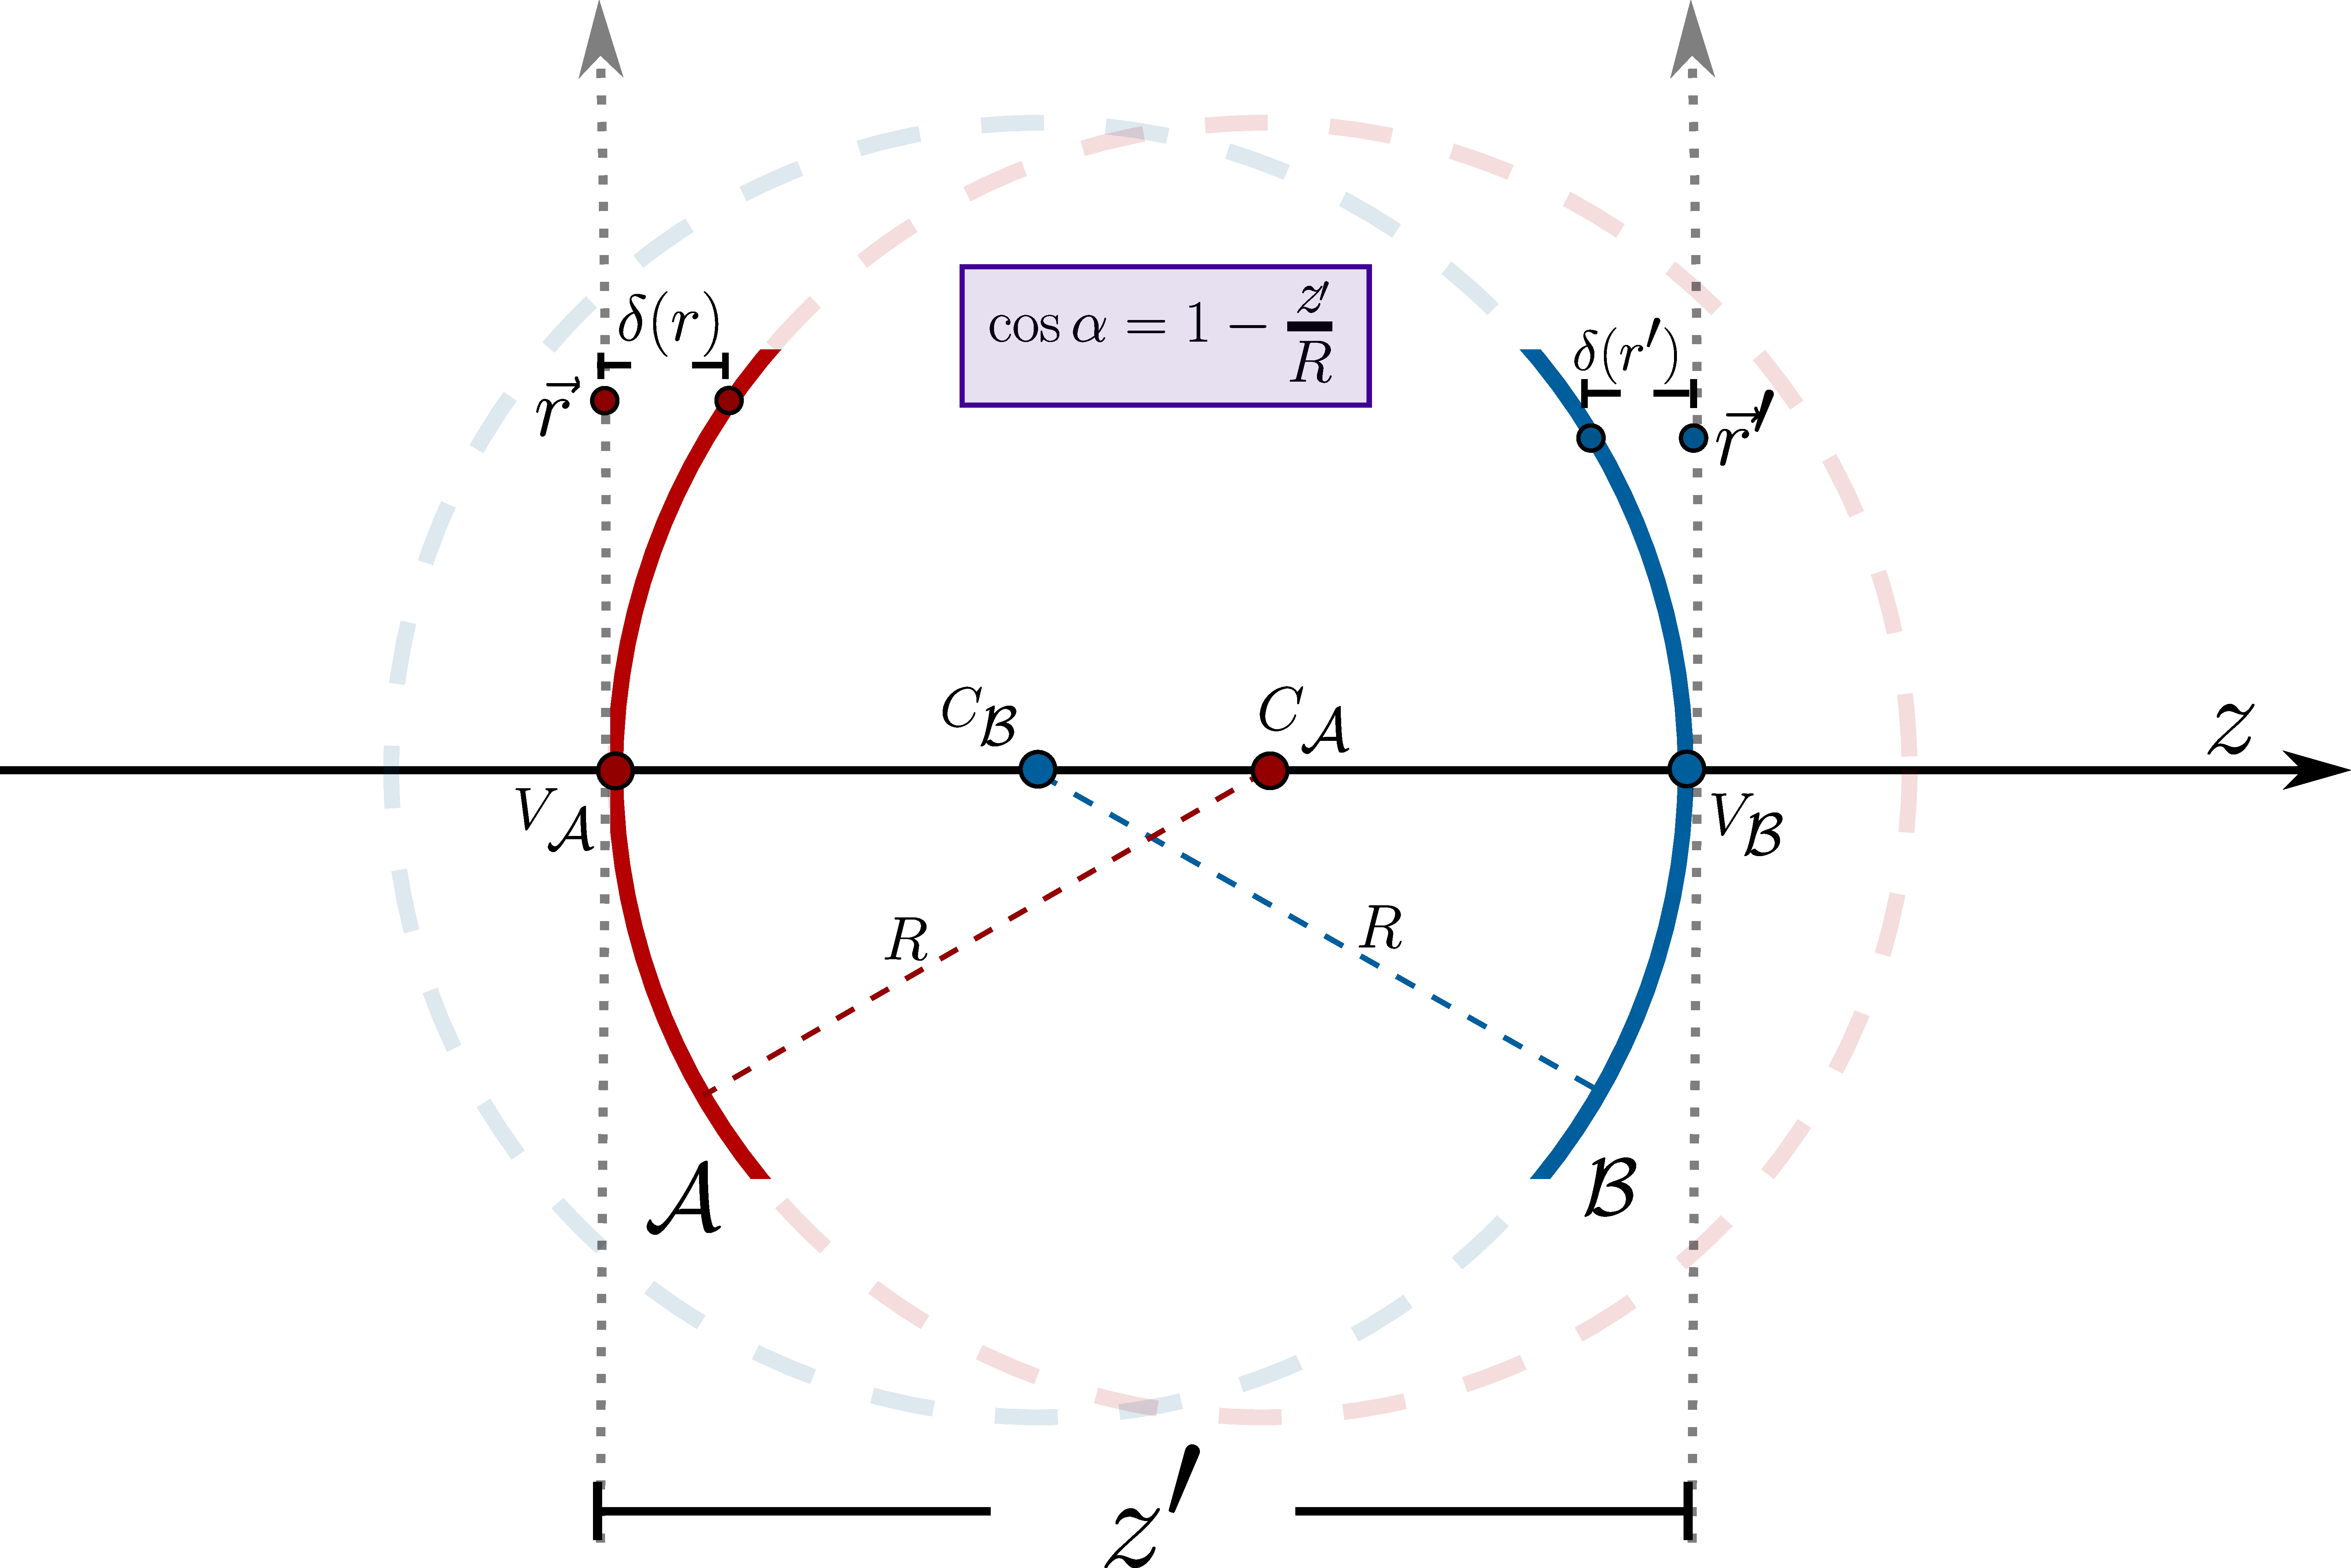
\includegraphics[width=0.8\textwidth]{Capitulo 1/Figuras/CardinalSpheres.pdf}
				\caption{Las dos esferas cardinales de radio $R$ asociadas a una propagación sobre
				la distancia $z$. El casquete emisor $\mathcal{A}$ es tangente a su plano en
				$V_{\mathcal{A}}$ con su centro de curvatura aguas abajo en $C_{\mathcal{A}}$, de
				abscisa $R$, y el casquete receptor $\mathcal{B}$ es tangente a su plano en
				$V_{\mathcal{B}}$ con su centro aguas arriba en $C_{\mathcal{B}}$, de abscisa
				$z-R$, de modo que los dos casquetes se curvan uno hacia el otro. La cantidad $\delta$ es la
				sagita \eqref{eq:FrFT:Sagitta}. El caso confocal de la
				Figura~\ref{fig:ConfocalSpheres} se recupera cuando $R = z$, ya que entonces
				$C_{\mathcal{A}}$ cae sobre $V_{\mathcal{B}}$ y $C_{\mathcal{B}}$ sobre
				$V_{\mathcal{A}}$.}
				\label{fig:CardinalSpheres}
			\end{figure}

			Con \eqref{eq:FrFT:Cardinals} los dos coeficientes cuadráticos colapsan en la única cantidad
			\begin{equation}\label{eq:FrFT:Q}
				Q = \frac{k}{2}\left(\frac{1}{z}-\frac{1}{R}\right),
			\end{equation}
			y la propagación se lee
			\begin{equation}\label{eq:FrFT:SphereToSphere}
				u_{\mathcal{B}}(\vec{r}\,') = \frac{e^{ikz}}{i\lambda z}\int_{\mathbb{R}^{2}} u_{\mathcal{A}}(\vec{r})\exp\left[iQ\left(r^{2}+r'^{2}\right)\right]\exp\left[-\frac{ik}{z}\,\vec{r}\cdot\vec{r}\,'\right]\mathrm{d}^{2}r,
			\end{equation}
			que ahora tiene exactamente la estructura de \eqref{eq:FrFT:Kernel2D} con coeficientes cuadrático y cruzado independientes. Repitiendo la identificación de la subsubsección anterior con las variables reducidas \eqref{eq:FrFT:Reduced},
			\begin{align}
				& Q\,\omega^{2} = \frac{\cot\alpha}{2} \quad\Longrightarrow\quad \cot\alpha = k\,\omega^{2}\left(\frac{1}{z}-\frac{1}{R}\right),\label{eq:FrFT:MatchQuad}\\
				& \frac{k}{z}\,\omega^{2} = \csc\alpha,\label{eq:FrFT:MatchCross}
			\end{align}
			y dividiendo \eqref{eq:FrFT:MatchQuad} entre \eqref{eq:FrFT:MatchCross} la escala $\omega$ se cancela una vez más,
			\begin{equation*}
				\cos\alpha = \frac{\cot\alpha}{\csc\alpha} = \frac{{\color{red}k\,\omega^{2}}\left(\dfrac{1}{z}-\dfrac{1}{R}\right)}{{\color{red}k\,\omega^{2}}\,\dfrac{1}{z}} = z\left(\frac{1}{z}-\frac{1}{R}\right),
			\end{equation*}
			de modo que obtenemos el resultado central
			\begin{equation}\label{eq:FrFT:Order}
				\boxed{\;\cos\alpha = 1 - \frac{z}{R}.\;}
			\end{equation}

			Esta vez no hay contradicción, porque el radio $R$ de los casquetes de referencia está a nuestra disposición. La longitud de escala se sigue de \eqref{eq:FrFT:MatchCross},
			\begin{equation}\label{eq:FrFT:Scale}
				\omega^{2} = \frac{z}{k\sin\alpha} = \frac{\lambda z}{2\pi\sin\alpha},
			\end{equation}
			y, eliminando $\alpha$ mediante \eqref{eq:FrFT:Order} y $\sin^{2}\alpha = 1-\cos^{2}\alpha$,
			\begin{equation*}
				\sin^{2}\alpha = {\color{red}1} - \left({\color{red}1} - \frac{2z}{R} + \frac{z^{2}}{R^{2}}\right) = \frac{z\left(2R-z\right)}{R^{2}} \quad\Longrightarrow\quad \sin\alpha = \frac{\sqrt{z\left(2R-z\right)}}{R},
			\end{equation*}
			cancelándose las dos unidades en rojo, de modo que la longitud de escala se expresa enteramente en términos de la geometría,
			\begin{equation}\label{eq:FrFT:ScaleExplicit}
				\omega^{2} = \frac{\lambda R}{2\pi}\sqrt{\frac{z}{2R-z}}.
			\end{equation}

		\subsubsection{La constante de normalización y el resultado final}

			Resta comparar las constantes. Cambiando variables en \eqref{eq:FrFT:SphereToSphere} según \eqref{eq:FrFT:Reduced}, de modo que $\mathrm{d}^{2}r = \omega^{2}\,\mathrm{d}^{2}u$,
			\begin{equation}\label{eq:FrFT:Reduced2}
				u_{\mathcal{B}}(\omega\vec{v}) = \frac{e^{ikz}\,\omega^{2}}{i\lambda z}\int_{\mathbb{R}^{2}} u_{\mathcal{A}}(\omega\vec{u})\exp\left[\frac{i}{2}\left(u^{2}+v^{2}\right)\cot\alpha - i\,\vec{u}\cdot\vec{v}\csc\alpha\right]\mathrm{d}^{2}u,
			\end{equation}
			y usando \eqref{eq:FrFT:Scale} el prefactor se simplifica a
			\begin{equation}\label{eq:FrFT:PrefactorOptics}
				\frac{\omega^{2}}{i\lambda z} = \frac{1}{i\,{\color{red}\lambda z}}\cdot\frac{{\color{red}\lambda z}}{2\pi\sin\alpha} = \frac{1}{2\pi i\sin\alpha} = \frac{-i}{2\pi\sin\alpha}.
			\end{equation}
			Por otra parte la constante de \eqref{eq:FrFT:Kernel2D}, reescrita mediante la identidad \eqref{eq:FrFT:ConstantEquiv}, es
			\begin{equation}\label{eq:FrFT:PrefactorFrFT}
				\frac{1-i\cot\alpha}{2\pi} = \frac{1}{2\pi}\cdot\frac{e^{-i\pi/2}e^{i\alpha}}{\sin\alpha} = \frac{-i\,e^{i\alpha}}{2\pi\sin\alpha}.
			\end{equation}
			Dividiendo \eqref{eq:FrFT:PrefactorOptics} entre \eqref{eq:FrFT:PrefactorFrFT},
			\begin{equation*}
				\frac{\;\dfrac{-i}{{\color{red}2\pi\sin\alpha}}\;}{\dfrac{-i\,e^{i\alpha}}{{\color{red}2\pi\sin\alpha}}} = \frac{-i}{-i}\,e^{-i\alpha} = e^{-i\alpha},
			\end{equation*}
			y por lo tanto, reuniendo todo, hemos demostrado el teorema.

			\begin{myteo}
				\textit{(La difracción de Fresnel como transformación fraccionaria de Fourier)} Sea el campo referido a dos casquetes esféricos cardinales de radio $R$ separados por la distancia $z$ a lo largo del eje, en el sentido de \eqref{eq:FrFT:Cardinals}, y sean las coordenadas transversales reducidas por la escala $\omega$ de \eqref{eq:FrFT:ScaleExplicit}. Entonces la propagación de Fresnel \eqref{Fresnel} es la transformación fraccionaria de Fourier
				\begin{equation}\label{eq:FrFT:MainResult}
					u_{\mathcal{B}}(\omega\vec{v}) = e^{i\left(kz - \alpha\right)}\left(\mathcal{F}_{\alpha}\,u_{\mathcal{A}}\right)(\vec{v}),
				\end{equation}
				cuyo orden está dado por $\cos\alpha = 1 - z/R$.
			\end{myteo}

			Es pertinente un comentario sobre la fase residual. Aparte del factor trivial $e^{ikz}$, que simplemente cuenta el camino óptico a lo largo del eje, la propagación deja atrás el factor $e^{-i\alpha}$ y nada más. Esto es una consecuencia directa de la normalización $1/(i\lambda z)$ de la integral de Fresnel \eqref{Fresnel}, aquella para la cual el núcleo tiende a $\delta(\vec{r}-\vec{r}\,')$ cuando $z\to0$; si la constante se hubiera escrito con el signo opuesto, habría aparecido un $\pi$ aditivo en el exponente de \eqref{eq:FrFT:MainResult} sin contenido físico alguno. Con la normalización correcta, el orden $\alpha$ es exactamente la fase de Gouy acumulada, punto al que volveremos.

			Probemos \eqref{eq:FrFT:MainResult} en los tres casos que podemos verificar de manera independiente.

			\begin{enumerate}
				\item \textbf{$z = 0$.} La ecuación \eqref{eq:FrFT:Order} da $\cos\alpha = 1$, de donde $\alpha = 0$ y $\mathcal{F}_{0} = \mathcal{I}$: el campo sobre el casquete receptor es el campo sobre el casquete emisor, como debe ser.
				\item \textbf{$z = R$.} Ahora $\cos\alpha = 0$, de donde $\alpha = \pi/2$ y la transformación es la transformación de Fourier ordinaria. Esto no es una coincidencia: cuando $z=R$ el casquete emisor tiene su centro en la abscisa $R = z$, que es el vértice del casquete receptor, y el casquete receptor tiene su centro en $z-R = 0$, que es el vértice del casquete emisor. Los dos casquetes son por lo tanto \textit{las esferas cardinales confocales} de la Figura~\ref{fig:cardinals}, y recuperamos exactamente el resultado de Fraunhofer \eqref{Fraunhofer} de la sección anterior. La descripción de campo lejano es el caso particular $\alpha = \pi/2$ de la presente.
				\item \textbf{$z = 2R$.} Aquí $\cos\alpha = -1$, de donde $\alpha = \pi$ y $\mathcal{F}_{\pi} = \mathcal{P}$: el campo sobre el casquete receptor es el campo sobre el casquete emisor invertido. Dos transformaciones de Fourier consecutivas invierten la imagen, y la geometría dice lo mismo.
			\end{enumerate}

			La ganancia en economía es considerable. En la descripción plano a plano, encadenar dos propagaciones de distancias $z_{1}$ y $z_{2}$ exige componer dos integrales de Fresnel, y el núcleo compuesto debe recalcularse cada vez. En la presente descripción la composición es la ley de índices \eqref{eq:FrFT:IndexLaw},
			\begin{equation}\label{eq:FrFT:Chaining}
				\mathcal{F}_{\alpha_{2}}\mathcal{F}_{\alpha_{1}} = \mathcal{F}_{\alpha_{1}+\alpha_{2}},
			\end{equation}
			de modo que la propagación se describe mediante la adición de ángulos. Las distancias $z$ no se suman de ninguna manera útil, pero los órdenes sí, y este es el sentido preciso en el cual $\alpha$, y no $z$, es el parámetro natural de la propagación paraxial libre.

		\subsubsection{Significado físico de un orden real}

			Cuando $\alpha$ es real, \eqref{eq:FrFT:Order} exige $\left|1-z/R\right|\leq 1$, es decir
			\begin{equation}\label{eq:FrFT:RealRange}
				0 \leq z \leq 2R,
			\end{equation}
			y el orden recorre monótonamente el intervalo $[0,\pi]$ conforme el casquete de observación se aleja. La lectura de $\alpha$ es entonces completamente transparente, y hay tres maneras equivalentes de enunciarla.

			\textit{Como un grado de difracción.} El orden mide cuán lejos ha viajado el campo desde el campo cercano hacia el campo lejano, en una escala en la cual $\alpha = 0$ es la propia abertura y $\alpha = \pi/2$ es su patrón de Fraunhofer. Un campo observado en $\alpha = \pi/4$ está a medio camino entre su propia distribución y su transformada de Fourier, en un sentido que no es metafórico sino exacto, ya que aplicar dos veces la misma transformación produce la transformada de Fourier. El continuo de regímenes intermedios que la aproximación de Fresnel describe solo implícitamente queda aquí etiquetado por un único número.

			\textit{Como una rotación del espacio de fase.} Por el teorema de Lohmann \citeyearpar{lohmann1993image}, establecido después con rigor por Mustard \citeyearpar{mustard1996fractional}, la transformación $\mathcal{F}_{\alpha}$ actúa sobre la distribución de Wigner del campo simplemente rotando el plano de la posición transversal y la frecuencia espacial transversal por el ángulo $\alpha$. La propagación libre entre esferas cardinales es por lo tanto una rotación rígida del espacio de fase, razón por la cual los órdenes se suman: las rotaciones se componen sumando ángulos. Esto también explica geométricamente por qué la propagación plano a plano no es una transformación fraccionaria, ya que en la descripción por planos la propagación es una cizalla del espacio de fase en lugar de una rotación.

			\textit{Como una fase de Gouy.} El factor residual $e^{-i\alpha}$ de \eqref{eq:FrFT:MainResult} no es accidental. Si en lugar de casquetes arbitrarios se eligen como superficies de referencia los frentes de onda de un haz gaussiano de rango de Rayleigh $z_{R}$, el orden que resulta del mismo cálculo es
			\begin{equation}\label{eq:FrFT:Gouy}
				\alpha = \arctan\!\left(\frac{z}{z_{R}}\right),
			\end{equation}
			que es precisamente la fase de Gouy acumulada del haz \citep{ozaktas1995fractional}. La identificación es satisfactoria, ya que \eqref{eq:FrFT:Gouy} tiende a $\pi/2$ cuando $z\to\infty$, recuperando una vez más el enunciado de que el campo lejano es la transformada de Fourier del campo cercano, y muestra que la misteriosa fase adicional de un haz enfocado no es sino el orden de la transformación fraccionaria que el haz ha sufrido.

			Debe subrayarse un punto, porque es una fuente frecuente de confusión. \textit{El orden no es una propiedad de la propagación por sí sola.} Es una propiedad del par formado por la propagación y los dos casquetes de referencia, ya que \eqref{eq:FrFT:Order} involucra tanto a $z$ como a $R$. Dada una distancia de propagación $z$, puede obtenerse cualquier orden que se desee eligiendo
			\begin{equation}\label{eq:FrFT:ChooseR}
				R = \frac{z}{1-\cos\alpha},
			\end{equation}
			y recíprocamente el mismo par de casquetes asigna órdenes distintos a distancias distintas. Lo que es intrínseco no es $\alpha$ sino la estructura de grupo: sean cuales sean los casquetes de referencia elegidos, la propagación está representada por un elemento del mismo grupo uniparamétrico.

		\subsubsection{Significado físico de un orden complejo}

			La condición \eqref{eq:FrFT:RealRange} es una restricción real, y es natural preguntarse qué sucede cuando se viola. Si el radio $R$ de los casquetes se mantiene fijo mientras la distancia de propagación excede $2R$, o si la propagación se hace correr hacia atrás de modo que $z<0$, entonces $\cos\alpha$ abandona el intervalo $[-1,1]$ y el orden se vuelve complejo. Escribiendo $\alpha = \alpha_{r} + i\alpha_{i}$ hay dos casos.

			Para $\cos\alpha > 1$, que corresponde a $z<0$ con $R>0$, el orden es puramente imaginario, $\alpha = i\beta$ con
			\begin{equation}\label{eq:FrFT:ImagOrder}
				\cosh\beta = 1 - \frac{z}{R}.
			\end{equation}

			Para $\cos\alpha < -1$, que corresponde a $z>2R$, el orden es $\alpha = \pi + i\beta$ con $\cosh\beta = z/R - 1$, cargando el $\pi$ aditivo la inversión de la imagen que ya encontramos en $z=2R$.

			La consecuencia sobre el núcleo es inmediata y físicamente elocuente. Tomando el primer caso y usando $\cot(i\beta) = -i\coth\beta$ y $\csc(i\beta) = -i\operatorname{csch}\beta$, el exponente de \eqref{eq:FrFT:Kernel2D} se convierte en
			\begin{align*}
				& \frac{i}{2}\left(u^{2}+v^{2}\right)\left(-i\coth\beta\right) - i\,\vec{u}\cdot\vec{v}\left(-i\operatorname{csch}\beta\right) = \\
				& \frac{1}{2}\left(u^{2}+v^{2}\right)\coth\beta - \vec{u}\cdot\vec{v}\operatorname{csch}\beta,
			\end{align*}
			que es \textit{enteramente real}. El núcleo ha dejado de ser un chirp puro y se ha convertido en una gaussiana real, y puesto que
			\begin{equation*}
				\coth\beta - \operatorname{csch}\beta = \frac{\cosh\beta - 1}{\sinh\beta} > 0 \qquad (\beta>0),
			\end{equation*}
			la forma cuadrática asociada es definida positiva, de modo que el núcleo crece en lugar de oscilar. Esta es la firma analítica de un problema mal planteado, y es exactamente lo que cabría esperar, ya que $z<0$ es retropropagación y la retropropagación amplifica sin límite el contenido de alta frecuencia espacial del campo. El orden complejo no se limita a describir la dificultad, la cuantifica: la parte imaginaria $\beta$ es el exponente de la amplificación gaussiana.

			De manera más general, un orden complejo admite tres lecturas físicas complementarias.

			\begin{enumerate}
				\item \textbf{Desde la teoría de grupos}, un orden real corresponde a un elemento elíptico del grupo de transformaciones canónicas lineales, es decir, a una rotación del espacio de fase, mientras que un orden complejo corresponde a un elemento que también contiene una compresión (\textit{squeeze}), es decir, una magnificación a lo largo de una dirección del espacio de fase y una compresión a lo largo de la otra. Un orden complejo anuncia por lo tanto que la transformación es una rotación compuesta con un escalamiento, y la parte imaginaria mide ese escalamiento.
				\item \textbf{Para haces gaussianos}, la curvatura del frente de onda no es un número real sino el parámetro complejo $q$ definido por $q^{-1} = R^{-1} - i\lambda/(\pi w^{2})$, donde $w$ es el radio del haz. Sustituyendo $q$ por $R$ en \eqref{eq:FrFT:Order} se obtiene automáticamente un orden complejo, cuya parte real es la rotación del espacio de fase y cuya parte imaginaria lleva la envolvente gaussiana del haz. Las transformaciones fraccionarias de orden complejo son, por esta razón, el lenguaje natural de la propagación de haces gaussianos, y fueron realizadas ópticamente por Shih \citeyearpar{shih1995optical} y por Bernardo y Soares \citeyearpar{bernardo1996optical}.
				\item \textbf{Para sistemas apodizados}, una abertura gaussiana $e^{-r^{2}/a^{2}}$ colocada en el haz contribuye exactamente con un factor gaussiano real del tipo que produce un orden complejo. La parte imaginaria del orden mide entonces la atenuación del contenido de $|\vec{u}|$ grande del campo, es decir, un filtrado pasa-bajas gaussiano en el dominio fraccionario, que en la imagen es una pérdida de resolución. Un orden complejo es, en esta lectura, el mecanismo de contabilidad para aberturas suaves y para pérdidas.
			\end{enumerate}

			Por último, debe subrayarse que un orden complejo nunca señala una imposibilidad física. Puesto que \eqref{eq:FrFT:ChooseR} muestra que el orden depende de los casquetes de referencia, cualquier propagación hacia adelante con $z>0$ puede describirse con un orden real simplemente eligiendo $R \geq z/2$. Lo que un orden complejo señala es que las superficies de referencia elegidas no son aquellas respecto a las cuales la propagación es una rotación pura. El caso límite de esta afirmación es el plano, para el cual $R\to\infty$ da $\cos\alpha\to1$ y, por \eqref{eq:FrFT:Scale}, $\omega\to\infty$: la transformación degenera, el ángulo de rotación colapsa a cero mientras la escala diverge, y recuperamos el teorema de la primera subsubsección de que la propagación de Fresnel plano a plano queda fuera de la familia fraccionaria de Fourier. Todo el contenido del resultado de Pellat-Finet es que la familia se recupera tan pronto se acepta mirar el campo sobre una esfera.


	\chapter{Teoría de la coherencia}\label{chap:Coherencia}
	\thispagestyle{empty}
	\vspace*{2cm}
	\begin{center}
		{\itshape\Huge La coherencia es el hilo que teje el orden a partir del caos de la luz aleatoria. \par}
		\vspace{1cm}
		\epigraph{``El tiempo avanza en la dirección en que las correlaciones aumentan''}{-- atribuido a Ludwig Boltzmann}
	\end{center}
	\clearpage

	\section{Contexto histórico de la teoría de la coherencia}

	En el fondo, la coherencia plantea una única pregunta, casi infantil: ¿cuánto se parece una cosa a otra, y sobrevive ese parecido con el paso del tiempo? Suena demasiado simple para importar, y sin embargo la búsqueda de una respuesta rigurosa a esa pregunta creció, a lo largo de tres siglos, hasta convertirse en una de las grandes ideas unificadoras de la física: un lenguaje que explica por qué algunas fuentes de luz producen franjas de interferencia nítidas mientras que otras no producen ninguna, por qué un haz láser se comporta de forma tan distinta a la llama de una vela, cómo los radioastrónomos fotografían la sombra de un agujero negro sin construir jamás un telescopio del tamaño de la Tierra, y por qué las delicadas superposiciones dentro de un computador cuántico son tan exasperantemente difíciles de mantener con vida. La historia de la coherencia es en realidad dos historias que crecieron por separado y solo más tarde descubrieron que hablaban de lo mismo: una comienza en una mesa de apuestas en la Francia del siglo XVII, y la otra comienza en un laboratorio de óptica a oscuras. Vale la pena seguir ambos hilos desde el principio.

	El primer hilo es la historia de la correlación, y comienza, apropiadamente, con una apuesta. En 1654 el noble y jugador Antoine Gombaud, más conocido como el Chevalier de Méré, escribió a Blaise Pascal preguntando cómo debían repartirse justamente las apuestas de una partida de dados interrumpida entre dos jugadores. La correspondencia resultante entre Pascal y Pierre de Fermat, en la que resolvieron la matemática de la esperanza y la combinatoria necesarias para responder tales preguntas, se considera generalmente el nacimiento de la teoría de la probabilidad. Sus ideas maduraron lentamente. En 1713, sesenta años más tarde, el libro póstumo de Jacob Bernoulli, \textit{Ars Conjectandi} \cite{bernoulli1713}, demostró la ley de los grandes números, el notable hecho de que si se repite un experimento aleatorio suficientes veces, la frecuencia observada de un resultado se estabiliza, cada vez con más fiabilidad, en torno a su probabilidad teórica verdadera. Un siglo más tarde todavía, en 1812, Pierre Simon Laplace reunió estos resultados dispersos, junto con su propia teoría de cómo debe actualizarse nuestra creencia ante nueva evidencia (lo que hoy llamamos inferencia bayesiana), en la monumental \textit{Théorie Analytique des Probabilités} \cite{laplace1812theorie}. Lo que aún faltaba en toda esta tradición era un número, una única cifra capaz de decir no solo cuán incierta es una cantidad, sino cuán fuertemente se mueven juntas dos cantidades distintas.

	Ese número faltante llegó por una vía inesperada: el muy práctico oficio de tratar con mediciones ruidosas. En 1809, tratando de ajustar las observaciones imperfectas y dispersas de las órbitas planetarias, Carl Friedrich Gauss introdujo el método de mínimos cuadrados en su \textit{Theoria Motus} \cite{gauss1809theoria}, una técnica construida enteramente sobre la idea de que los errores se agrupan estadísticamente en torno a la verdad. Décadas más tarde, en la década de 1880, el polímata Francis Galton, fascinado por cuán fuertemente la estatura de un hijo tiende a seguir la de sus padres, acuñó la palabra misma ``correlación'' para describir precisamente este tipo de tendencia conjunta \cite{galton1888correlations}. Le correspondió a su alumno Karl Pearson, en 1896, convertir la intuición de Galton en una fórmula precisa: el coeficiente de correlación de Pearson \cite{pearson1896regression}, un único número, siempre entre menos uno y más uno, que indica de un vistazo si dos cantidades marchan juntas, se separan, o se ignoran por completo. Por primera vez, el parecido entre dos cosas podía medirse en lugar de simplemente percibirse.

	El segundo hilo, mientras tanto, se desarrollaba casi por completo sin referencia al primero, en el estudio de la luz misma. En 1801, Thomas Young dejó caer luz solar a través de dos rendijas estrechas y la vio pintar una hilera de bandas claras y oscuras en una pantalla detrás de ellas \cite{young1804bakerian}, la firma inconfundible de dos ondas que a veces se refuerzan y a veces se cancelan mutuamente. Para que esas franjas aparecieran, la luz que salía de las dos rendijas tenía que mantener una relación de fase estable y confiable consigo misma, una propiedad para la que nadie tenía todavía un nombre, aunque todos podían ver su huella en la pantalla. Entre 1815 y 1820, Augustin Jean Fresnel construyó la teoría matemática completa de la luz como onda transversal, y con ella la interferencia y la polarización dejaron de ser curiosidades para convertirse en consecuencias de una única imagen física. Y sin embargo un misterio persistía silenciosamente. El haz de Young, recién dividido a partir de una sola rendija estrecha, producía franjas hermosamente. Pero la luz de día ordinaria, o la luz de una vela, o la del Sol mismo, jamás producían nada semejante cuando simplemente se les dejaba interferir con una copia retardada de sí mismas más allá de cierta separación. Algo en la luz real y cotidiana era distinto de la onda idealizada y perfectamente regular que describía la matemática de Fresnel, y durante cien años nadie pudo decir exactamente qué.

	La respuesta, cuando finalmente llegó en el siglo XX, es que las fuentes de luz ordinarias no son en absoluto ondas únicas y ordenadas. Un filamento caliente, una llama, o la superficie del Sol es una enorme multitud de átomos independientes, cada uno emitiendo su propio destello breve de luz y luego callando, completamente desacompasado de sus vecinos, de modo que la onda global forma y reforma su fase miles de millones de veces por segundo de una manera que, a todos los efectos prácticos, es aleatoria. Describir correctamente semejante luz significaba casar las dos tradiciones separadas que habían crecido de forma aislada: la maquinaria estadística de Pascal, Gauss, Galton y Pearson debía injertarse en la óptica ondulatoria de Young y Fresnel. Ese injerto es exactamente lo que la palabra ``coherencia'' designa hoy: no si una onda tiene una fase, toda onda la tiene, sino si esa fase permanece suficientemente predecible, durante suficiente tiempo y sobre una región suficientemente amplia, como para dejar un rastro visible cuando se hace que la onda interfiera con una copia de sí misma.

	El paso matemático decisivo se dio en la década de 1930. En 1934 el físico neerlandés Pieter Hendrik van Cittert resolvió cómo cambian las correlaciones estadísticas de la luz proveniente de una fuente incoherente y extendida, una estrella distante, por ejemplo, a medida que esa luz se aleja de la fuente \cite{vancittert1934}, y en 1938 Frits Zernike afinó y generalizó el resultado hasta el teorema que hoy lleva ambos nombres \cite{zernike1938}. El teorema de van Cittert-Zernike hace una afirmación hermosamente contraintuitiva: una luz que comienza siendo completamente incoherente, con cada punto de la fuente parpadeando independientemente de todos los demás, se vuelve medible y predeciblemente más coherente por el mero hecho de recorrer una gran distancia. Esto no es una nota al pie menor. Es el principio físico que permite a los astrónomos medir el tamaño angular de estrellas demasiado pequeñas para que cualquier telescopio las resuelva directamente, comparando la luz recogida en dos puntos separados y observando cómo se desvanecen las franjas a medida que crece la separación, exactamente el truco que Albert Michelson y Francis Pease usaron en 1920 para medir el diámetro de la gigante roja Betelgeuse \cite{michelson1921diameter}. Décadas después, ese mismo teorema, escalado de un puñado de metros a una red de antenas de radio que abarca todo el planeta, es lo que permitió a la colaboración del Telescopio del Horizonte de Sucesos reconstruir, en 2019, la primera imagen directa de un agujero negro.

	La teoría clásica de la coherencia encontró su forma definitiva y madura en el trabajo de Max Born y Emil Wolf, cuyo tratado \textit{Principles of Optics} \cite{born1999principles} reunió cada hebra en un solo objeto, la función de coherencia mutua, que simplemente mide cuán correlacionada está la onda luminosa entre dos puntos del espacio y dos instantes de tiempo. Comprimidas dentro de esa única función están las dos cualidades que de verdad interesan a un experimentador: la coherencia temporal, esencialmente cuán puro es el color de la luz y durante cuánto tiempo mantiene un ritmo estable consigo misma, y la coherencia espacial, cuán fielmente la onda se mantiene acompasada a lo largo de una región extendida en lugar de solo en un punto. Leonard Mandel y Wolf ampliaron más tarde esta imagen en el tratado completo \textit{Optical Coherence and Quantum Optics} \cite{mandel1995optical}, afinando las nociones prácticas de tiempo de coherencia y longitud de coherencia que hoy todo laboratorio da por sentadas. Nada de esto quedó confinado al tablero. El interferómetro de Michelson de la década de 1890 ya explotaba la coherencia temporal para medir longitudes de onda con una precisión que ninguna regla podía igualar, y la invención del láser en 1960, cuya luz es coherente en un grado que ninguna fuente natural alcanza jamás, convirtió la coherencia de un tema de fascinación teórica en el principio de funcionamiento detrás de las comunicaciones por fibra óptica, la metrología de precisión, la holografía y la medicina moderna.

	Tampoco la coherencia pertenece solo a la óptica. Dondequiera que muchas partes independientes de un sistema puedan hacerse oscilar al unísono, aparece algo con exactamente la misma anatomía matemática. En física de la materia condensada, la superconductividad es, en el fondo, un fenómeno de coherencia: por debajo de una temperatura crítica, una enorme población de electrones apareados se bloquea en una única fase cuántica compartida a través de toda una muestra macroscópica, razón por la cual una supercorriente fluye sin resistencia alguna. La resonancia magnética nuclear y la resonancia magnética de imágenes construida sobre ella funcionan inclinando miles de millones de espines nucleares hacia una precesión común y coherente, y observando luego, con exquisita sensibilidad, cuán rápido decae ese ritmo compartido. Todo reloj atómico, y con él el sistema de posicionamiento global entero, depende de un oscilador cuya fase permanece coherente durante todo el tiempo humanamente alcanzable. La coherencia, en resumen, no es una peculiaridad de la luz; es lo que permite que innumerables actores independientes, electrones, espines, átomos o fotones, se comporten, brevemente y con fragilidad, como uno solo.

	Mientras toda esta maquinaria clásica se consolidaba, una historia completamente distinta y más extraña se desarrollaba en el mundo cuántico. Su escena inicial tuvo lugar en 1956, cuando Robert Hanbury Brown y Richard Twiss, tratando de medir los tamaños angulares de las estrellas con detectores de radio y luego ópticos, descubrieron que los fotones que llegaban de una fuente térmica a dos detectores separados no eran independientes: tendían a llegar en pequeños grupos correlacionados \cite{hanburybrown1956correlation}. El resultado parecía a muchos físicos de la época sencillamente imposible. Los fotones, se suponía, debían comportarse como partículas clásicas e independientes una vez detectados, y ninguna correlación semejante debía sobrevivir al acto de la medición; siguió una controversia real y animada antes de que el efecto fuera aceptado. Desenredarlo correctamente requería una teoría plenamente cuántica de la coherencia, y esa teoría fue provista en 1963, casi simultánea e independientemente, por Roy Glauber \cite{glauber1963quantum} y George Sudarshan \cite{sudarshan1963equivalence}. Glauber introdujo los estados coherentes, los estados cuánticos de la luz que se comportan tan cerca como la mecánica cuántica lo permite de las ondas clásicas de Fresnel, y definió toda una jerarquía de funciones de correlación cuánticas capaces de explicar rigurosamente el agrupamiento de Hanbury Brown y Twiss, y de predecir su imagen especular, el antiagrupamiento de fotones, un comportamiento tan tercamente no clásico que ninguna teoría ondulatoria de la luz podría jamás reproducirlo, confirmado más tarde en el laboratorio. Sudarshan, trabajando desde una dirección distinta, encontró la frontera matemática precisa, hoy llamada representación de Glauber-Sudarshan, que separa la luz cuya naturaleza cuántica puede ignorarse con seguridad de aquella para la cual no puede. Por esta teoría cuántica de la coherencia óptica, Glauber recibió el Premio Nobel en 2005, y el campo que fundó es lo que hoy llamamos óptica cuántica.

	La coherencia cuántica resultó importar por razones que van mucho más allá del conteo de fotones. Es la coherencia cuántica, la delicada superposición de fase fija de muchos estados posibles a la vez, lo que hace que un bit cuántico sea fundamentalmente distinto de uno ordinario, y es la pérdida de esa coherencia por el contacto inevitable con el entorno, un proceso que los físicos llaman decoherencia, lo que explica por qué el mundo cotidiano a nuestro alrededor luce tan tercamente clásico aunque esté construido a partir de partes cuánticas. Mantener la coherencia con vida el tiempo suficiente para que sea útil es, hasta el día de hoy, el mayor obstáculo de ingeniería que se interpone entre los computadores cuánticos de hoy y los del mañana. La misma idea reaparece en la materia más fría que los físicos saben producir: en 1995 Eric Cornell, Carl Wieman y Wolfgang Ketterle enfriaron nubes de átomos a temperaturas de nanokelvin y observaron a millones de ellos colapsar en un único estado cuántico compartido, un condensado de Bose-Einstein, en efecto una enorme onda de materia coherente, un logro reconocido con el Premio Nobel en 2001. Incluso alcanza a la biología: experimentos cuidadosos sobre los complejos captadores de luz que las plantas y ciertas bacterias usan para capturar la luz solar han encontrado que la coherencia cuántica en la transferencia de esa energía sobrevive, asombrosamente, durante fracciones medibles de segundo a temperatura ambiente, sugiriendo que la evolución pudo haber tropezado con la coherencia cuántica y explotado mucho antes de que los físicos le dieran un nombre.

	Uniendo las imágenes estadística y ondulatoria de la coherencia, tanto clásica como cuántica, hay una única pieza de matemática: el teorema de Wiener-Khinchin, desarrollado independientemente por Norbert Wiener en 1930 \cite{wiener1930generalized} y Aleksandr Khinchin en 1934 \cite{khinchin1934korrelationstheorie}, que establece que la correlación de una señal fluctuante consigo misma y la manera en que la energía de esa señal se distribuye en frecuencia son simplemente dos caras del mismo objeto, traducidas la una a la otra mediante una transformada de Fourier. Es, como mostrarán los capítulos posteriores, la bisagra matemática silenciosa sobre la que gira todo el tema.

	En el siglo XXI la coherencia ha adquirido una identidad más: hoy se entiende, y se cuantifica formalmente, como un recurso físico genuino, algo que puede crearse, gastarse y agotarse casi como la energía o el entrelazamiento, con sus propias reglas de contabilidad rigurosas dentro de la teoría más amplia de la información cuántica \cite{baumgratz2014quantifying}. Vista de principio a fin, la historia de la coherencia recorre desde un argumento del siglo XVII sobre dados, pasando por la estadística de la estatura heredada y la interferencia de la luz solar, hasta la formación de imágenes de un agujero negro y el frágil funcionamiento interno de un procesador cuántico. En su forma clásica explica por qué las estrellas titilan como lo hacen, por qué un láser puede cortar acero mientras que una antorcha no puede, y por qué un interferómetro del tamaño de un planeta puede fotografiar algo que ningún telescopio individual pudo jamás. En su forma cuántica explica por qué el mundo de los átomos se siente tan distinto del mundo de las mesas y las sillas, y hoy se sitúa en el centro mismo del esfuerzo por construir tecnologías que piensen y se comuniquen de maneras que ninguna máquina clásica pudo jamás. La coherencia, ya se cuente en tiradas de dados correlacionadas, ondas de luz que interfieren o qubits entrelazados, es en último término siempre lo mismo: el orden, sobreviviendo breve y notablemente en un mundo que constantemente conspira para borrarlo.

\section{¿Cómo se cuantifica la similaridad estadística?}

	Supongamos que tenemos un fenómeno completamente aleatorio, como la radiación electromagnética emitida por una bombilla incandescente que no está en equilibrio termodinámico, el número de automóviles en alguna ciudad capital a lo largo del día, el movimiento de un ion en un plasma, o algo tan simple como lanzar una pelota al aire en condiciones no ideales.

	Cuando deseamos analizar estadísticamente un único objeto o variable aleatoria, aparecen las herramientas familiares: la densidad de probabilidad, el valor medio, la desviación estándar, la curtosis, etcétera. ¿Qué ocurre cuando queremos estudiar al menos dos variables aleatorias y cómo se relacionan? Cuando deseamos estudiar la estadística de dos o más variables aleatorias debemos estudiar la similaridad estadística entre ellas; pero la similaridad estadística es un concepto bastante amplio, pues podemos tener similaridad en los valores medios, o en las desviaciones estándar, o en las densidades de probabilidad. Para abordar este problema volvemos al álgebra lineal.

	Si tenemos dos vectores $\vec{A},\vec{B} \in \mathbb{R}^n$, el producto punto $\vec{A}\cdot\vec{B}$ se interpreta como la magnitud de la proyección de $\vec{A}$ sobre $\vec{B}$ y viceversa; también puede leerse como \textit{cuánto de $\vec{A}$ yace a lo largo de $\vec{B}$}.

	Vale la pena detenerse en lo que esa operación en verdad hace mecánicamente, porque toda la teoría de la coherencia está construida sobre este único gesto. Escrito componente a componente, el producto punto es
	\begin{equation}\label{eq:DotComponents}
		\vec{A}\cdot\vec{B} = \sum_{i=1}^{n} A_i B_i,
	\end{equation}
	es decir, \textit{multiplíquense las dos listas entrada por entrada y súmense los resultados}. Nada más. Y sin embargo el signo de cada término individual ya lleva exactamente la información que buscamos: siempre que $A_i$ y $B_i$ se inclinan hacia el mismo lado, su producto es positivo y empuja la suma hacia arriba; siempre que se inclinan hacia lados opuestos, el producto es negativo y la arrastra hacia abajo. Si los dos vectores tienden a coincidir a lo largo de la mayoría de sus componentes, los términos positivos dominan y el total resulta grande; si sistemáticamente discrepan, el total resulta grande pero negativo; y si coinciden con la misma frecuencia con que discrepan, los términos se cancelan mutuamente en la suma y el total colapsa a casi cero. Así, ``multiplicar los pares y sumar'' es ya, por sí solo, un medidor de similaridad, y todo lo que sigue en este capítulo es ese mismo gesto aplicado a objetos progresivamente más ricos.

	Este comportamiento puede extrapolarse a espacios vectoriales continuos, donde suele emplearse la noción de producto interno. El paso es más pequeño de lo que parece: una función es simplemente un vector con un continuo de componentes, pues en lugar de la lista finita $A_1,A_2,\dots,A_n$ ahora llevamos los valores $f_A(x)$, uno para cada $x$. El índice $i$ se convierte en la etiqueta $x$, la suma sobre un índice discreto se convierte en una integral sobre uno continuo, y el producto punto se convierte en el producto interno. Si $f_A , f_B$ son dos elementos del espacio de Hilbert $L^2(\mathbb{R})$ de funciones de cuadrado integrable de una variable real, puede definirse un producto interno como

	\begin{equation}\label{eq:ProdIn}
		\braket{f_A,f_B} = \int_\mathbb{R} f_A^*(x)f_B(x) W(x)\,dx,
	\end{equation}

	donde el conjugado complejo en el primer factor es lo que mantiene a $\braket{f_A,f_A}$ real y no negativo incluso cuando las funciones son complejas, como lo serán los campos ópticos de este capítulo, y donde $W(x)$ es alguna función de peso.\footnote{$W(x)$ recibe este nombre porque, como su nombre indica, otorga un peso a cada valor que el integrando pueda tomar; no hay contribuciones uniformes, sino que cada valor posible del integrando dentro del dominio contribuye ponderado por el valor de $W$ en ese punto.} La interpretación sigue siendo válida: esto puede leerse como cuánto coincide la función $f_A$ sobre todos los reales con la función $f_B$ sobre todos los reales.

	Para llegar a la noción de correlación a partir del álgebra lineal usamos un poco de notación bra-ket, donde el ket $\ket{f_A}$ representa un vector de un espacio de Hilbert $L^2$ arbitrario y el bra $\bra{f_A}$ representa un elemento del dual del mismo espacio de Hilbert,\footnote{El espacio de Hilbert es un caso particular de los espacios $L^p$, el espacio de funcionales Lebesgue-integrables de norma $p$; para Hilbert $p=2$, y tiene la propiedad de que el dual de $L^2$ es también $L^2$, lo que permite que la mecánica cuántica surja naturalmente en este espacio.} y el producto interno de un estado consigo mismo, $\braket{f_A,f_A}= \braket{f_A|f_A}$, acumula la probabilidad de encontrar el sistema en cualquier lugar; es el integrando $|f_A(q)|^2$, más que la integral completada, el que juega el papel de la densidad de probabilidad de encontrar $f_A$ en un estado $q \pm \triangle q$, donde $q$ representa alguna coordenada generalizada. Supongamos que $f_A,f_B \in L^2$ tienen la forma

	\begin{equation}
		\ket{f_A} = \hat{A}\ket{\Psi_A}, \quad \ket{f_B} = \hat{B}\ket{\Psi_B},
	\end{equation}

	donde $\hat{A},\hat{B}$ son los operadores de las magnitudes físicas de $\ket{\Psi_A},\ket{\Psi_B}$, de modo que podemos interpretar $\ket{f_A},\ket{f_B}$ como las funciones de onda gobernadas por su valor esperado. Usando el producto interno \eqref{eq:ProdIn} con función de peso unitaria, $W=1$, el producto interno se lee

	\begin{equation}
		\braket{f_A | f_B} = \int_{\mathbb{R}^n} \hat{A}\hat{B} \braket{\Psi_A|\Psi_B}\, d^nq = \int_{\mathbb{R}^n} \hat{A}\hat{B}\, P(A;B)\, d^nq,
	\end{equation}

	donde vemos que la similaridad entre $\ket{f_A}$ y $\ket{f_B}$ puede verse como el producto de $\hat{A}$ con $\hat{B}$ multiplicado por la densidad de probabilidad de tener los estados $A$ y $B$.\footnote{Este último paso es deliberadamente heurístico: estamos tratando los operadores como si pudieran simplemente sacarse del producto interno y reemplazarse por los valores que miden, lo cual solo es legítimo cuando actúan sobre sus propios autoestados. El propósito aquí no es una derivación sino un puente, para hacer plausible de dónde viene la definición que sigue; el tratamiento riguroso pertenece a \cite{mandel1995optical}.} Es decir, la similaridad, o cuán \textit{correlacionadas} están dos variables, puede verse como la integral del producto de las variables multiplicada por su densidad de probabilidad conjunta.

	Con esta analogía en mente podemos entender la correlación como una primera medida de la similaridad entre una o más variables a través del espacio y del tiempo. Si $x_1(\vec{r},t_1), x_2(\vec{r}',t_2)$ son dos variables aleatorias y $p_2(x_1,t_1;x_2,t_2)$ es la densidad de probabilidad conjunta, entonces la correlación entre $x_1,x_2$ se define como

	\begin{equation}\label{eq:CorrFunc}
		\Gamma(\vec{r},\vec{r}';t_1,t_2) = E\left\{ x_1(\vec{r},t_1) x_2^*(\vec{r}',t_2)\right\}
		= \int\!\!\int x_1 x_2^* \; p_2(x_1,t_1;x_2,t_2)\, dx_1 dx_2,
	\end{equation}

	es decir, como el promedio de ensamble de $x_1\cdot x_2^*$, ponderado por cuán probable es que cada par de valores ocurra conjuntamente. La conjugación se coloca aquí en el segundo factor para concordar con la convención usada para la función de coherencia en la siguiente sección; para variables reales no hace nada en absoluto, y para las complejas simplemente conjuga a $\Gamma$ en su totalidad, sin afectar ninguna magnitud que nos vaya a interesar.

	Estructuralmente este es el mismo objeto que hemos venido construyendo todo este tiempo. La suma sobre componentes en \eqref{eq:DotComponents} se ha convertido simplemente en un promedio sobre el ensamble, y el papel de la función de peso $W$ en \eqref{eq:ProdIn} lo desempeña ahora la densidad de probabilidad conjunta $p_2$, que es el peso natural a usar cuando las ``componentes'' que se emparejan son los resultados posibles de un experimento aleatorio en lugar de las entradas de una lista. La correlación, en otras palabras, es el producto punto de dos variables aleatorias, tomado en el único sentido disponible cuando las cantidades involucradas se niegan a quedarse quietas.

	El mismo argumento del signo que convirtió al producto punto en un medidor de similaridad nos dice ahora cómo leer $\Gamma$, y vale la pena exponer los tres casos explícitamente. Si las dos variables suben y bajan juntas, de modo que son grandes en los mismos instantes y pequeñas en los mismos instantes, entonces el producto $x_1 x_2^*$ es predominantemente positivo, cada realización del experimento contribuye con el mismo signo, y el promedio sobrevive como un número positivo grande. Si se mueven en oposición estricta, una alcanzando su pico cada vez que la otra alcanza su valle, el producto es predominantemente negativo y el promedio sobrevive como un número negativo grande, lo cual es igualmente informativo: la anticorrelación perfecta es una forma de similaridad perfecta, simplemente con un signo adjunto. Pero si las dos variables no saben nada la una de la otra, entonces por cada realización en la que el producto resulta ser positivo hay, en algún lugar del ensamble, una realización igualmente probable en la que resulta negativo, las contribuciones se aniquilan mutuamente, y el promedio colapsa a cero. \textbf{El promediado no es, por tanto, un tecnicismo incidental sino el mecanismo entero}: es precisamente lo que destruye los términos que no llevan información compartida mientras permite que los términos que sí la llevan se acumulen.

	Dos rasgos de la definición \eqref{eq:CorrFunc} merecen un comentario, porque ambos difieren del coeficiente de Pearson visto en la introducción histórica. El primero es que no hemos restado los valores medios antes de multiplicar. Restarlos produciría la covarianza, que pregunta cómo conspiran las \textit{fluctuaciones} en torno al promedio; conservarlos, como hacemos aquí, pregunta por la cantidad total, y para los campos ópticos de este capítulo la distinción felizmente se desvanece, pues un campo térmico oscila simétricamente en torno a cero y su media se anula por sí sola. El segundo es que no hemos dividido por nada, de modo que $\Gamma$ todavía lleva las unidades físicas de los campos con los que fue construida y su magnitud depende de cuán intensa resulta ser la luz, no solo de cuán similar es. Una correlación de $10^{-6}$ entre dos haces débiles puede representar un acuerdo mucho más estrecho que una correlación de la unidad entre dos haces potentes. Reparar esto, dividiendo $\Gamma$ por su propio valor a separación nula, que es precisamente la intensidad, de modo que el resultado sea un número puro confinado entre cero y uno que mida similaridad y solo similaridad, es exactamente el paso que convierte a la función de correlación en el \textit{grado complejo de coherencia}, y es el punto hacia el que trabaja la siguiente sección.

\section{Variables aleatorias}\label{sec:RandomVariables}

	En la sección anterior hablamos libremente de variables aleatorias, de densidades de probabilidad conjuntas y de promedios de ensamble, y lo hicimos a propósito, porque el objetivo allí era hacer plausible la definición de la función de correlación, no justificarla. Esa deuda debe pagarse ahora. La teoría de la coherencia es, de principio a fin, una teoría \textit{sobre} promedios, y un promedio que no está definido con precisión no define nada con precisión. Peor aún, los objetos que manipularemos no son promedios de números sino promedios sobre una colección infinita de historias de campo enteras, y para tales objetos la intuición ingenua no es meramente imprecisa, sino que en ocasiones es sencillamente errónea.

	El propósito de esta sección es, por tanto, construir la noción de variable aleatoria desde los cimientos, en el lenguaje de la teoría de la medida en el que fue formulada por Kolmogórov \citep{kolmogorov1933grundbegriffe}, y luego aplicarla al campo electromagnético vectorial, construyendo explícitamente el espacio de probabilidad sobre el cual vive toda la teoría que sigue. Cada ingrediente recibirá su lectura física a medida que aparezca, porque cada uno de ellos corresponde a algo que un óptico hace en un laboratorio.

	\subsection{El espacio muestral y el significado físico de un evento}

		\begin{myDef}
			\textit{(Espacio muestral)} Un \textit{espacio muestral} es un conjunto no vacío $\Omega$. Sus elementos $\omega\in\Omega$ se llaman \textit{resultados elementales} o \textit{puntos muestrales}.
		\end{myDef}

		La tentación es leer $\omega$ como un número, y es esencial resistirla. En óptica un resultado elemental no es un valor de campo ni una medición; es una \textit{realización} completa de la fuente, es decir, una historia espaciotemporal entera que el campo podría haber tenido. Una lámpara térmica contiene del orden de $10^{20}$ átomos radiando independientemente, cada uno con un instante de emisión y una fase inicial que ni controlamos ni conocemos. Una asignación particular de todos esos detalles microscópicos, junto con todo lo que se sigue de ella mediante las ecuaciones de Maxwell, es un $\omega$. El conjunto de todas esas asignaciones es $\Omega$.

		Esta es precisamente la imagen que mostrará la Figura~\ref{fig:randomvar} en la sección siguiente, donde se dibujan varias curvas $^{(i)}E(\vec{r},t)$ una encima de otra: cada curva es un $\omega$, y la etiqueta $i$ es solo un recurso de contabilidad, pues en general $\Omega$ es no numerable. Lo que el laboratorio entrega en una tarde cualquiera es un único $\omega$, elegido por la naturaleza y no revelado a nosotros. La totalidad de la óptica estadística consiste en extraer afirmaciones sobre $\Omega$ a partir del acceso a uno solo de sus puntos.

		\begin{myDef}
			\textit{(Evento)} Un \textit{evento} es un subconjunto $A\subseteq\Omega$.
		\end{myDef}

		El contenido físico de esta definición es que un evento es un \textbf{enunciado sobre la realización que puede declararse verdadero o falso}. El enunciado ``el campo en $\vec{r}_{0}$ en el instante $t_{0}$ superó el valor $E_{0}$'' no es un número; es el conjunto de todas las realizaciones para las cuales ocurre que eso es el caso. Decir que el evento ocurrió es decir que el $\omega$ que la naturaleza seleccionó pertenece a ese subconjunto. Eventos y enunciados son la misma cosa vista desde dos lados, y esta identificación es lo que permite construir la probabilidad a partir de la teoría de conjuntos.

	\subsection{La sigma-álgebra, o qué preguntas pueden formularse}

		\begin{myDef}
			\textit{(Sigma-álgebra)} Una \textit{sigma-álgebra} sobre $\Omega$ es una colección $\mathcal{F}$ de subconjuntos de $\Omega$ tal que
			\begin{enumerate}
				\item $\Omega\in\mathcal{F}$,
				\item si $A\in\mathcal{F}$ entonces $A^{c} = \Omega\setminus A\in\mathcal{F}$,
				\item si $A_{1},A_{2},A_{3},\dots\in\mathcal{F}$ entonces $\bigcup_{n=1}^{\infty}A_{n}\in\mathcal{F}$.
			\end{enumerate}
			El par $(\Omega,\mathcal{F})$ se llama \textit{espacio medible}.
		\end{myDef}

		Una sigma-álgebra parece una pieza de contabilidad y es, de hecho, un enunciado físico. Es el \textit{catálogo de preguntas admisibles}, la lista de enunciados a los que la teoría está preparada para asignar una probabilidad, y los tres axiomas son exactamente las tres propiedades que cualquier catálogo honesto de preguntas debe tener.

		El primero dice que la pregunta ``¿ocurrió algo en absoluto?'' es admisible. El segundo dice que si podemos preguntar si un evento ocurrió, podemos preguntar si no ocurrió, lo cual es la expresión formal del hecho de que un aparato capaz de detectar algo es, por ese mismo hecho, capaz de detectar su ausencia. El tercero dice que si cada una de una sucesión de preguntas es admisible, también lo es la pregunta de si al menos una de ellas se cumple.

		La palabra \textit{numerable} en el tercer axioma no es una conveniencia técnica sino una restricción física genuina, y merece señalarse. Cualquier protocolo experimental real es una \textit{sucesión} de operaciones: se registra una lectura, luego otra, luego otra. Ningún laboratorio ha realizado jamás una cantidad no numerable de operaciones, y la teoría está construida para no prometer nada sobre lo que ocurriría si se pudiera.

		Cabría preguntarse por qué no tomamos simplemente $\mathcal{F}$ como la colección de \textit{todos} los subconjuntos de $\Omega$ y asunto terminado. La respuesta es que no se nos permite hacerlo. Vitali demostró en 1905 \citep{vitali1905problema} que en la recta real existen conjuntos tan patológicos que ninguna noción de tamaño invariante bajo traslación puede asignárseles sin contradicción. Si insistiéramos en medirlo todo nos veríamos forzados a la inconsistencia, y la sigma-álgebra es precisamente el dispositivo que mantiene semejantes monstruos fuera de la teoría mientras conserva todo conjunto sobre el que un físico tendría ocasión de preguntar alguna vez.

		El ejemplo que necesitaremos constantemente es el siguiente.

		\begin{myDef}
			\textit{(Sigma-álgebra de Borel)} La \textit{sigma-álgebra de Borel} $\mathcal{B}(\mathbb{R}^{n})$ es la sigma-álgebra más pequeña sobre $\mathbb{R}^{n}$ que contiene todos los conjuntos abiertos.
		\end{myDef}

		Físicamente, $\mathcal{B}(\mathbb{R})$ está generada por las preguntas ``¿la lectura está entre $a$ y $b$?'', junto con todo lo que puede construirse a partir de una cantidad numerable de tales preguntas mediante negación y unión. Esta es exactamente la clase de preguntas que un detector real, que tiene una resolución finita y reporta un intervalo en lugar de un punto, es capaz de responder. La sigma-álgebra de Borel no es una abstracción impuesta a la física; es la transcripción matemática de lo que hace un instrumento graduado.

	\subsection{Medida, la medida de Lebesgue y la medida de probabilidad}

		\begin{myDef}
			\textit{(Medida)} Una \textit{medida} sobre un espacio medible $(\Omega,\mathcal{F})$ es una función $\mu:\mathcal{F}\to[0,\infty]$ tal que $\mu(\emptyset)=0$ y tal que, para toda sucesión $A_{1},A_{2},\dots$ de elementos de $\mathcal{F}$ disjuntos dos a dos,
			\begin{equation}\label{eq:CountableAdditivity}
				\mu\left(\bigcup_{n=1}^{\infty}A_{n}\right) = \sum_{n=1}^{\infty}\mu(A_{n}).
			\end{equation}
			La terna $(\Omega,\mathcal{F},\mu)$ es un \textit{espacio de medida}.
		\end{myDef}

		Una medida es una manera consistente de asignar un \textit{tamaño}. La condición \eqref{eq:CountableAdditivity} es la aditividad numerable, y no establece nada más exótico que el hecho de que el tamaño de un todo ensamblado a partir de piezas separadas es la suma de los tamaños de las piezas. Eso es lo que la palabra tamaño significa operacionalmente, y una función que lo violara no merecería el nombre.

		Entre todas las medidas hay una que la propia geometría del espacio distingue.

		\begin{myDef}
			\textit{(Medida de Lebesgue)} La \textit{medida de Lebesgue} $\lambda$ es la única medida invariante bajo traslación sobre $\mathcal{B}(\mathbb{R}^{n})$ que satisface $\lambda\left(\prod_{j=1}^{n}[a_{j},b_{j}]\right) = \prod_{j=1}^{n}(b_{j}-a_{j})$.
		\end{myDef}

		La medida de Lebesgue \citep{lebesgue1902integrale} es la forma matemática de las palabras \textit{longitud}, \textit{área}, \textit{volumen} y \textit{duración}. Toda integral que hemos escrito hasta ahora en estos apuntes ha sido una integral contra $\lambda$: cuando integramos sobre una abertura en la teoría de la difracción estábamos midiendo \textit{cuánta abertura hay}, y cuando integramos sobre el tiempo de respuesta de un detector estamos midiendo \textit{cuánto tiempo miramos}. La medida de Lebesgue conoce la extensión del dominio y no sabe absolutamente nada sobre probabilidad.

		Vale la pena insistir en esta separación, porque en la teoría de la coherencia ambas medidas aparecen a la vez y hacen trabajos por completo distintos. \textbf{La medida de Lebesgue registra cuánto tiempo integró el detector y cuán grande era la abertura; la medida de probabilidad registra cuán probable era cada realización de la fuente.} El promedio temporal de un único haz es una integral contra $\lambda$ sobre el eje del tiempo; el promedio de ensamble sobre realizaciones es una integral contra $P$ sobre $\Omega$. Estas son operaciones distintas sobre espacios distintos, y el hecho de que tan a menudo coincidan no es una trivialidad sino un teorema con hipótesis, al que volvemos al final de esta sección.

		La medida de Lebesgue también suministra la justificación que faltaba a las densidades de la sección anterior. Cuando en \eqref{eq:CorrFunc} escribimos $p_{2}(x_{1},t_{1};x_{2},t_{2})\,dx_{1}dx_{2}$ estábamos suponiendo tácitamente que la medida de probabilidad sobre el espacio de valores es absolutamente continua respecto de $\lambda$, de modo que, por el teorema de Radon-Nikodým \citep{nikodym1930generalisation}, posee una densidad. Esa es una hipótesis física y no una formalidad: afirma que ningún valor de campo ocurre con probabilidad estrictamente positiva, es decir, que la fuente no tiene rasgos infinitamente agudos. Un láser perfectamente monocromático y perfectamente estabilizado la violaría, pues su distribución estaría concentrada en un círculo del plano complejo, un conjunto de medida de Lebesgue nula, y no existiría densidad alguna respecto del plano.

		\begin{myDef}
			\textit{(Espacio de probabilidad)} Una \textit{medida de probabilidad} es una medida $P$ con $P(\Omega)=1$. La terna $(\Omega,\mathcal{F},P)$ se llama \textit{espacio de probabilidad}.
		\end{myDef}

		La normalización $P(\Omega)=1$ es el enunciado de que la fuente hace \textit{algo}: ocurre alguna realización, y las alternativas listadas en $\Omega$ son exhaustivas. La aditividad numerable, leída ahora en $P$, es el enunciado de que las alternativas mutuamente excluyentes tienen probabilidades que se suman.

		Aquí se encuentra el comentario físico crucial de esta subsección. \textbf{La medida de probabilidad es donde reside la física de la fuente.} Una lámpara térmica, un láser y un emisor de un solo fotón bien pueden compartir el mismo $\Omega$ y la misma $\mathcal{F}$, pues los tres podrían en principio producir cualquiera de las mismas historias de campo; lo que los distingue es que ponderan esas historias de forma distinta. Especificar una fuente es especificar $P$, y toda afirmación que la teoría de la coherencia haga sobre la luz es, en último análisis, una afirmación sobre $P$.

	\subsection{Variables aleatorias y el significado de la medibilidad}

		\begin{myDef}
			\textit{(Variable aleatoria)} Sea $(\Omega,\mathcal{F},P)$ un espacio de probabilidad y $(S,\mathcal{S})$ un espacio medible. Una aplicación $X:\Omega\to S$ es una \textit{variable aleatoria} si es \textit{medible}, es decir, si
			\begin{equation}\label{eq:Measurability}
				X^{-1}(B) = \left\{\omega\in\Omega : X(\omega)\in B\right\}\in\mathcal{F}
				\qquad\text{para todo } B\in\mathcal{S}.
			\end{equation}
		\end{myDef}

		Dos cosas deben decirse sobre esta definición, y ambas suelen decirse demasiado deprisa.

		La primera es que \textbf{una variable aleatoria no es una variable que sea aleatoria}. Es una función perfectamente determinista. Una vez fijada la realización $\omega$, $X(\omega)$ es un elemento definido de $S$, sin nada caprichoso en ello. Toda la aleatoriedad reside en la selección de $\omega$, es decir, en nuestra ignorancia de qué realización ha producido la naturaleza. El campo en un punto del espaciotiempo no fluctúa porque esté indeciso; es definido en cada realización y simplemente no sabemos en cuál realización estamos.

		La segunda es que la condición de medibilidad \eqref{eq:Measurability} es el enunciado matemático de que \textbf{el instrumento es un instrumento legítimo}. Exige que la pregunta ``¿cayó la lectura dentro de $B$?'' sea una de las preguntas admisibles de $\mathcal{F}$. Una aplicación no medible sería un aparato que reporta una respuesta a una pregunta a la que la teoría se niega a asignar una probabilidad, lo cual es una manera cortés de decir que reporta números que no significan nada. La medibilidad es la licencia para existir.

		Dado que el resultado $\omega$ es inaccesible, lo que un experimento en realidad reconstruye no es $P$ sino su imagen.

		\begin{myDef}
			\textit{(Ley de una variable aleatoria)} La \textit{ley} o \textit{distribución} de $X$ es la medida de probabilidad $P_{X}$ sobre $(S,\mathcal{S})$ definida por el empuje hacia adelante
			\begin{equation}\label{eq:PushForward}
				P_{X}(B) = P\left(X^{-1}(B)\right), \qquad B\in\mathcal{S}.
			\end{equation}
			Si $P_{X}$ es absolutamente continua respecto de la medida de Lebesgue, su derivada de Radon-Nikodým $p = \mathrm{d}P_{X}/\mathrm{d}\lambda$ es la \textit{densidad de probabilidad} de $X$.
		\end{myDef}

		La ley es lo que un histograma estima. Dos fuentes construidas sobre espacios muestrales por completo distintos pueden poseer leyes idénticas para un observable dado, y son entonces indistinguibles mediante ese observable sin importar cuánto tiempo se mida. La densidad $p$ que aquí aparece es exactamente la $p_{2}$ que se usó sin disculpas en \eqref{eq:CorrFunc}.

		\begin{myDef}
			\textit{(Esperanza)} La \textit{esperanza} de una variable aleatoria integrable $X$ es la integral de Lebesgue de $X$ sobre el espacio de probabilidad,
			\begin{equation}\label{eq:Expectation}
				E\{X\} = \int_{\Omega}X(\omega)\,\mathrm{d}P(\omega)
				= \int_{S}x\,\mathrm{d}P_{X}(x) = \int_{S}x\,p(x)\,\mathrm{d}\lambda(x),
			\end{equation}
			siendo la segunda igualdad el cambio de variable inducido por \eqref{eq:PushForward}.
		\end{myDef}

		La ecuación \eqref{eq:Expectation} legitima retroactivamente la definición \eqref{eq:CorrFunc} de la función de correlación. Lo que allí se escribió como un promedio de ensamble y lo que se escribió como una integral contra una densidad conjunta no son dos definiciones que resulten coincidir; son una única definición, dada sobre $\Omega$, y su imagen sobre el espacio de valores bajo el empuje hacia adelante. La primera forma es conceptualmente primaria y la segunda es la que podemos calcular.

		Hay ahora una recompensa que vale la pena enunciar explícitamente, porque convierte la analogía central de la sección anterior de una metáfora en un teorema. Consideremos el conjunto de variables aleatorias de segundo momento finito,

		\begin{equation}\label{eq:L2Omega}
			L^{2}(\Omega,\mathcal{F},P) = \left\{X : \Omega\to\mathbb{C} \;\middle|\; E\left\{|X|^{2}\right\}<\infty\right\},
		\end{equation}
		equipado con el producto interno

		\begin{equation}\label{eq:L2InnerProduct}
			\braket{X,Y} = E\left\{XY^{*}\right\}.
		\end{equation}

		Este es un espacio de Hilbert, y comparando \eqref{eq:L2InnerProduct} con la definición \eqref{eq:CorrFunc} de la función de correlación vemos que \textbf{la función de correlación es un producto interno}, no por analogía sino literalmente, en el espacio de variables aleatorias de energía finita. El producto punto con el que comenzó la sección anterior no era un paralelo ilustrativo; era el mismo objeto, esperando a que se nombrara el espacio. La función de peso $W$ de \eqref{eq:ProdIn} se ha convertido en la medida $P$, y la suma sobre componentes de \eqref{eq:DotComponents} se ha convertido en la integral sobre $\Omega$.

		De esta identificación se sigue de inmediato una desigualdad, y es la que hace significativo al grado normalizado de coherencia. La desigualdad de Cauchy-Schwarz en $L^{2}(\Omega,\mathcal{F},P)$ se lee

		\begin{equation}\label{eq:CauchySchwarzProb}
			\left|E\left\{XY^{*}\right\}\right|^{2} \leq E\left\{|X|^{2}\right\}\,E\left\{|Y|^{2}\right\},
		\end{equation}
		de modo que la correlación de dos variables aleatorias jamás puede exceder la media geométrica de sus intensidades. Cuando dividimos por esa media geométrica, como se anticipó al final de la sección anterior, el resultado es un número puro comprendido entre cero y uno. Es, literalmente, el coseno del ángulo entre dos vectores en un espacio de Hilbert, y esta es la razón por la que un grado de coherencia mayor que la unidad no es simplemente algo nunca observado sino algo imposible.

	\subsection{Procesos estocásticos}

		Una única variable aleatoria describe el campo en un punto del espaciotiempo. Para describirlo en todas partes a la vez necesitamos una familia.

		\begin{myDef}
			\textit{(Proceso estocástico)} Sea $T$ un conjunto de índices. Un \textit{proceso estocástico} es una familia $\{X_{\tau}\}_{\tau\in T}$ de variables aleatorias definidas sobre un espacio de probabilidad común $(\Omega,\mathcal{F},P)$, equivalentemente una aplicación $X:T\times\Omega\to S$ tal que $X(\tau,\cdot)$ es medible para cada $\tau\in T$.
		\end{myDef}

		Un proceso estocástico admite dos lecturas, y toda la intuición del tema consiste en sostener ambas a la vez \citep{doob1953stochastic}. Si fijamos el índice $\tau$ y dejamos variar a $\omega$, obtenemos una variable aleatoria: un corte \textit{vertical} a través de la Figura~\ref{fig:randomvar}, que compara todas las realizaciones en un instante. Si en cambio fijamos $\omega$ y dejamos variar a $\tau$, obtenemos una única función del índice, llamada \textit{trayectoria muestral} o \textit{realización}: un corte \textit{horizontal}, es decir, una de las curvas individuales de la figura. El experimentalista observa cortes horizontales y la teoría habla de cortes verticales, y reconciliar ambos es el problema práctico central de la óptica estadística.

	\subsection{El espacio de probabilidad del campo electromagnético}

		Ya podemos llevar a cabo la construcción para la que se preparaba toda esta sección, y construir explícitamente el espacio de probabilidad sobre el cual opera la teoría de la coherencia. Sea $D\subseteq\mathbb{R}^{3}\times\mathbb{R}$ la región del espaciotiempo en la que pretendemos describir el campo, y recordemos que el campo es un objeto complejo de tres componentes, la señal analítica $\vec{\mathcal{E}} = (\mathcal{E}_{x},\mathcal{E}_{y},\mathcal{E}_{z})$.

		Como espacio muestral tomamos

		\begin{equation}\label{eq:FieldSampleSpace}
			\Omega = \left\{\omega : D\to\mathbb{C}^{3} \;\middle|\; \omega \text{ satisface las ecuaciones de Maxwell en } D\right\},
		\end{equation}
		es decir, el conjunto de historias de campo admisibles. La restricción es esencial y es física: la naturaleza no selecciona funciones arbitrarias del espaciotiempo sino solo aquellas compatibles con la dinámica. \textbf{La aleatoriedad entra a través de las fuentes y jamás a través de la propagación}, que permanece exactamente tan determinista como lo era en los capítulos anteriores. Una medida de probabilidad sobre un campo óptico es una medida sobre el espacio de soluciones de las ecuaciones de Maxwell, y esta es la razón por la cual, como veremos en una subsección posterior, la coherencia misma obedece una ecuación de onda.

		Con esta elección el campo se convierte en la aplicación más simple imaginable, a saber, la evaluación de una función en un punto,

		\begin{equation}\label{eq:EvaluationMap}
			\mathcal{E}_{j}(\vec{r},t) : \Omega\to\mathbb{C}, \qquad \omega\mapsto\omega_{j}(\vec{r},t),
			\qquad j\in\{x,y,z\},
		\end{equation}
		de modo que para cada punto del espaciotiempo y cada componente cartesiana el campo es una variable aleatoria compleja, y el vector $\vec{\mathcal{E}}(\vec{r},t):\Omega\to\mathbb{C}^{3}$ es una variable aleatoria con valores en $\mathbb{C}^{3}$. El campo entero es el proceso estocástico indexado por $T = D\times\{x,y,z\}$.

		Equipamos a continuación a $\Omega$ con la \textit{sigma-álgebra cilíndrica} $\mathcal{F}$, generada por los conjuntos

		\begin{equation}\label{eq:CylinderSets}
			C = \left\{\omega\in\Omega \;\middle|\; \left(\omega(\vec{r}_{1},t_{1}),\dots,\omega(\vec{r}_{n},t_{n})\right)\in B\right\},
			\qquad B\in\mathcal{B}(\mathbb{C}^{3n}),
		\end{equation}
		para toda colección finita de puntos del espaciotiempo y todo conjunto de Borel $B$.

		La lectura física de \eqref{eq:CylinderSets} es el comentario más importante de esta sección. \textbf{Un conjunto cilíndrico es exactamente un enunciado que puede verificarse colocando un número finito de detectores en un número finito de puntos del espaciotiempo y observando sus lecturas.} Ningún experimento ha medido jamás un campo en todas partes; todo experimento lo muestrea en un número finito de lugares y un número finito de instantes. La sigma-álgebra generada por los conjuntos cilíndricos es, por tanto, la colección de todos los enunciados decidibles mediante sucesiones numerables de mediciones finitas, es decir, la colección de todos los enunciados que un experimento óptico puede llegar a resolver. La construcción cilíndrica no es una conveniencia matemática, es la transcripción de la práctica experimental.

		Resta colocar una medida de probabilidad sobre este espacio enorme, y sería desesperanzador intentarlo directamente. El teorema de extensión de Kolmogórov \citep{kolmogorov1933grundbegriffe} muestra que es innecesario.

		\begin{myteo}
			\textit{(Teorema de extensión de Kolmogórov)} Dada una familia de distribuciones de dimensión finita $P_{(\vec{r}_{1},t_{1}),\dots,(\vec{r}_{n},t_{n})}$ sobre $\mathbb{C}^{3n}$, una para cada colección finita de puntos del espaciotiempo, que sea consistente bajo permutación de los puntos y bajo marginalización sobre cualquiera de ellos, existe una única medida de probabilidad $P$ sobre la sigma-álgebra cilíndrica $\mathcal{F}$ cuyas marginales de dimensión finita son las dadas.
		\end{myteo}

		El contenido físico es liberador. \textbf{Para especificar una fuente basta con especificar la estadística conjunta de cualquier conjunto finito de lecturas de detectores}, y esta es precisamente la información a la que un experimento puede acceder. Nunca tenemos que decir qué hace $P$ al monstruoso espacio de todas las historias de campo; decimos cuál es la distribución conjunta de dos detectores, y de tres, y así sucesivamente, cuidando únicamente que estas prescripciones no se contradigan entre sí, y Kolmogórov garantiza que se entrelazan en un único objeto consistente. El espacio de probabilidad de un campo óptico se construye exactamente con la información que un laboratorio puede suministrar.

		Suponemos finalmente, y esta es la última hipótesis de la construcción, que

		\begin{equation}\label{eq:FiniteEnergy}
			E\left\{\left|\mathcal{E}_{j}(\vec{r},t)\right|^{2}\right\}<\infty
			\qquad \text{para todo } j \text{ y todo } (\vec{r},t)\in D,
		\end{equation}
		que es el enunciado de que la densidad de energía media es finita, es decir, de que la fuente no radia una potencia infinita. Físicamente es inobjetable, y matemáticamente es exactamente la hipótesis que coloca a cada componente del campo dentro del espacio de Hilbert \eqref{eq:L2Omega}. A partir de este punto, cada componente del campo en cada punto del espaciotiempo es un vector en uno y el mismo espacio de Hilbert, y la geometría de ese espacio es la geometría de la coherencia.

		Podemos ya definir, habiéndose dado significado a cada símbolo, el objeto que estudia el resto de este capítulo. Para dos puntos del espaciotiempo y dos componentes cartesianas,

		\begin{equation}\label{eq:CoherenceTensor}
			\Gamma_{jk}(\vec{r},t;\vec{r}\,',t') = E\left\{\mathcal{E}_{j}(\vec{r},t)\,\mathcal{E}_{k}^{*}(\vec{r}\,',t')\right\}
			= \braket{\mathcal{E}_{j}(\vec{r},t),\mathcal{E}_{k}(\vec{r}\,',t')},
		\end{equation}
		una matriz $3\times3$ asociada a cada par de puntos del espaciotiempo, siendo el producto interno el de \eqref{eq:L2InnerProduct}. Esta es la generalización vectorial de la función de correlación \eqref{eq:CorrFunc}, y tres de sus propiedades se siguen de inmediato de la construcción.

		\begin{enumerate}
			\item \textbf{Simetría hermítica.} Intercambiando los dos puntos y los dos índices y conjugando,
			\begin{equation}\label{eq:GammaHermitian}
				\Gamma_{kj}^{*}(\vec{r}\,',t';\vec{r},t) = E\left\{\mathcal{E}_{k}^{*}(\vec{r}\,',t')\,\mathcal{E}_{j}(\vec{r},t)\right\} = \Gamma_{jk}(\vec{r},t;\vec{r}\,',t'),
			\end{equation}
			ya que la conjugación puede introducirse dentro de la esperanza, que es una integral de una función compleja.
			\item \textbf{No negatividad definida.} Para cualquier conjunto finito de puntos del espaciotiempo etiquetados por $m$ y cualesquiera coeficientes complejos $a_{j}^{(m)}$,
			\begin{equation}\label{eq:GammaPositive}
				\sum_{m,n}\sum_{j,k}a_{j}^{(m)}a_{k}^{(n)*}\,\Gamma_{jk}(m;n)
				= E\left\{\left|\sum_{m}\sum_{j}a_{j}^{(m)}\mathcal{E}_{j}(m)\right|^{2}\right\}\geq 0,
			\end{equation}
			porque la esperanza de una cantidad no negativa es no negativa. Físicamente esto dice que ninguna superposición de componentes de campo, en cualesquiera puntos, puede llevar intensidad negativa.
			\item \textbf{Correlación acotada.} Por \eqref{eq:CauchySchwarzProb},
			\begin{equation}\label{eq:GammaBound}
				\left|\Gamma_{jk}(\vec{r},t;\vec{r}\,',t')\right|^{2} \leq \Gamma_{jj}(\vec{r},t;\vec{r},t)\;\Gamma_{kk}(\vec{r}\,',t';\vec{r}\,',t'),
			\end{equation}
			que es lo que permite confinar al grado normalizado de coherencia al intervalo $[0,1]$.
		\end{enumerate}

		Vale la pena notar dónde encaja la polarización en todo esto. Evaluando \eqref{eq:CoherenceTensor} en un único punto del espaciotiempo, $\vec{r}=\vec{r}\,'$ y $t=t'$, las entradas diagonales $\Gamma_{jj}$ dan la intensidad media que lleva cada componente cartesiana mientras que las entradas fuera de la diagonal miden la correlación entre componentes, y la matriz resultante es exactamente la matriz de polarización introducida en el capítulo sobre polarización de la óptica electromagnética clásica. \textbf{La polarización es coherencia entre las componentes del campo en un punto; la coherencia propiamente dicha es correlación entre el campo en puntos distintos.} Son el mismo tensor leído en dos regímenes diferentes, y esta es la razón por la cual es posible en absoluto un tratamiento unificado de la coherencia y la polarización \citep{wolf2007introduction}.

	\subsection{Estacionariedad, ergodicidad y el derecho a medir}

		Queda una pregunta, y es la pregunta de la que depende la relevancia experimental de todo lo anterior. La esperanza \eqref{eq:Expectation} es un promedio sobre $\Omega$, y $\Omega$ no es accesible: la naturaleza nos entrega una realización. Aquello sobre lo que sí podemos promediar es el tiempo, a lo largo de esa única realización. ¿Bajo qué condiciones coinciden ambos?

		La primera condición concierne a la invariancia de la fuente.

		\begin{myDef}
			\textit{(Estacionariedad)} Sea $\theta_{\tau}:\Omega\to\Omega$ el desplazamiento temporal definido por $(\theta_{\tau}\omega)(\vec{r},t) = \omega(\vec{r},t+\tau)$. El campo es \textit{estacionario} si $P$ es invariante bajo todo desplazamiento de este tipo,
			\begin{equation}\label{eq:StationarityMeasure}
				P\left(\theta_{\tau}^{-1}A\right) = P(A) \qquad \text{para todo } A\in\mathcal{F} \text{ y todo } \tau\in\mathbb{R}.
			\end{equation}
		\end{myDef}

		Esta es la forma en teoría de la medida del enunciado, dado de manera más elemental en la siguiente sección, de que las propiedades estadísticas de la luz no dependen de cuándo elegimos empezar a contar el tiempo. Una lámpara encendida hace una hora y dejada en paz es estacionaria; una fuente pulsada no lo es. Su consecuencia inmediata es que el tensor de coherencia \eqref{eq:CoherenceTensor} solo puede depender de los dos instantes a través de su diferencia, $\Gamma_{jk}(\vec{r},\vec{r}\,';t,t') = \Gamma_{jk}(\vec{r},\vec{r}\,';\tau)$ con $\tau=t'-t$, lo cual es lo que hace posible, en primer lugar, el teorema de Wiener-Khinchin de la sección siguiente.

		La segunda condición es más fuerte y concierne a la indescomponibilidad de la fuente.

		\begin{myDef}
			\textit{(Ergodicidad)} Un campo estacionario es \textit{ergódico} si todo evento invariante bajo desplazamiento es trivial, es decir, si $\theta_{\tau}^{-1}A = A$ para todo $\tau$ implica $P(A)=0$ o $P(A)=1$.
		\end{myDef}

		Físicamente, la ergodicidad dice que la fuente no puede dividirse en dos subensambles que jamás se comuniquen. Si pudiera, una única realización quedaría atrapada para siempre en uno de ellos y jamás podría informar sobre el otro. Cuando se cumple, el teorema ergódico de Birkhoff \citep{birkhoff1931proof} se aplica y da el resultado que necesitamos,

		\begin{equation}\label{eq:Ergodic}
			\lim_{T\to\infty}\frac{1}{2T}\int_{-T}^{T}\mathcal{E}_{j}(\vec{r},t)\,\mathcal{E}_{k}^{*}(\vec{r}\,',t+\tau)\,\mathrm{d}t
			= E\left\{\mathcal{E}_{j}(\vec{r},t)\,\mathcal{E}_{k}^{*}(\vec{r}\,',t+\tau)\right\}
		\end{equation}
		para casi toda realización $\omega$.

		La ecuación \eqref{eq:Ergodic} es la licencia, y la única licencia, para reemplazar el promedio de ensamble inaccesible por el promedio temporal accesible de un único haz, y es la razón por la cual toda la teoría es experimentalmente significativa y no meramente elegante. Nótese, finalmente, qué son los dos lados de \eqref{eq:Ergodic}: a la izquierda una integral contra la medida de Lebesgue sobre el eje del tiempo, a la derecha una integral contra la medida de probabilidad sobre $\Omega$. Las dos medidas que con tanto cuidado mantuvimos separadas al comienzo de esta sección se encuentran aquí, en una única identidad, y la ergodicidad es precisamente la hipótesis bajo la cual pueden intercambiarse. Con esta hipótesis en mano podemos volver a la física y definir la función de coherencia misma.

\section{Función de coherencia}

	El concepto de función de coherencia es, a nivel matemático, idéntico al de la función de correlación dada en la ecuación \eqref{eq:CorrFunc}; ambas representan correlaciones. Sin embargo, coherencia es un término ampliamente usado en el estudio de la radiación electromagnética; veamos un poco por qué es así.

	\begin{figure}[htbp]
		\centering
		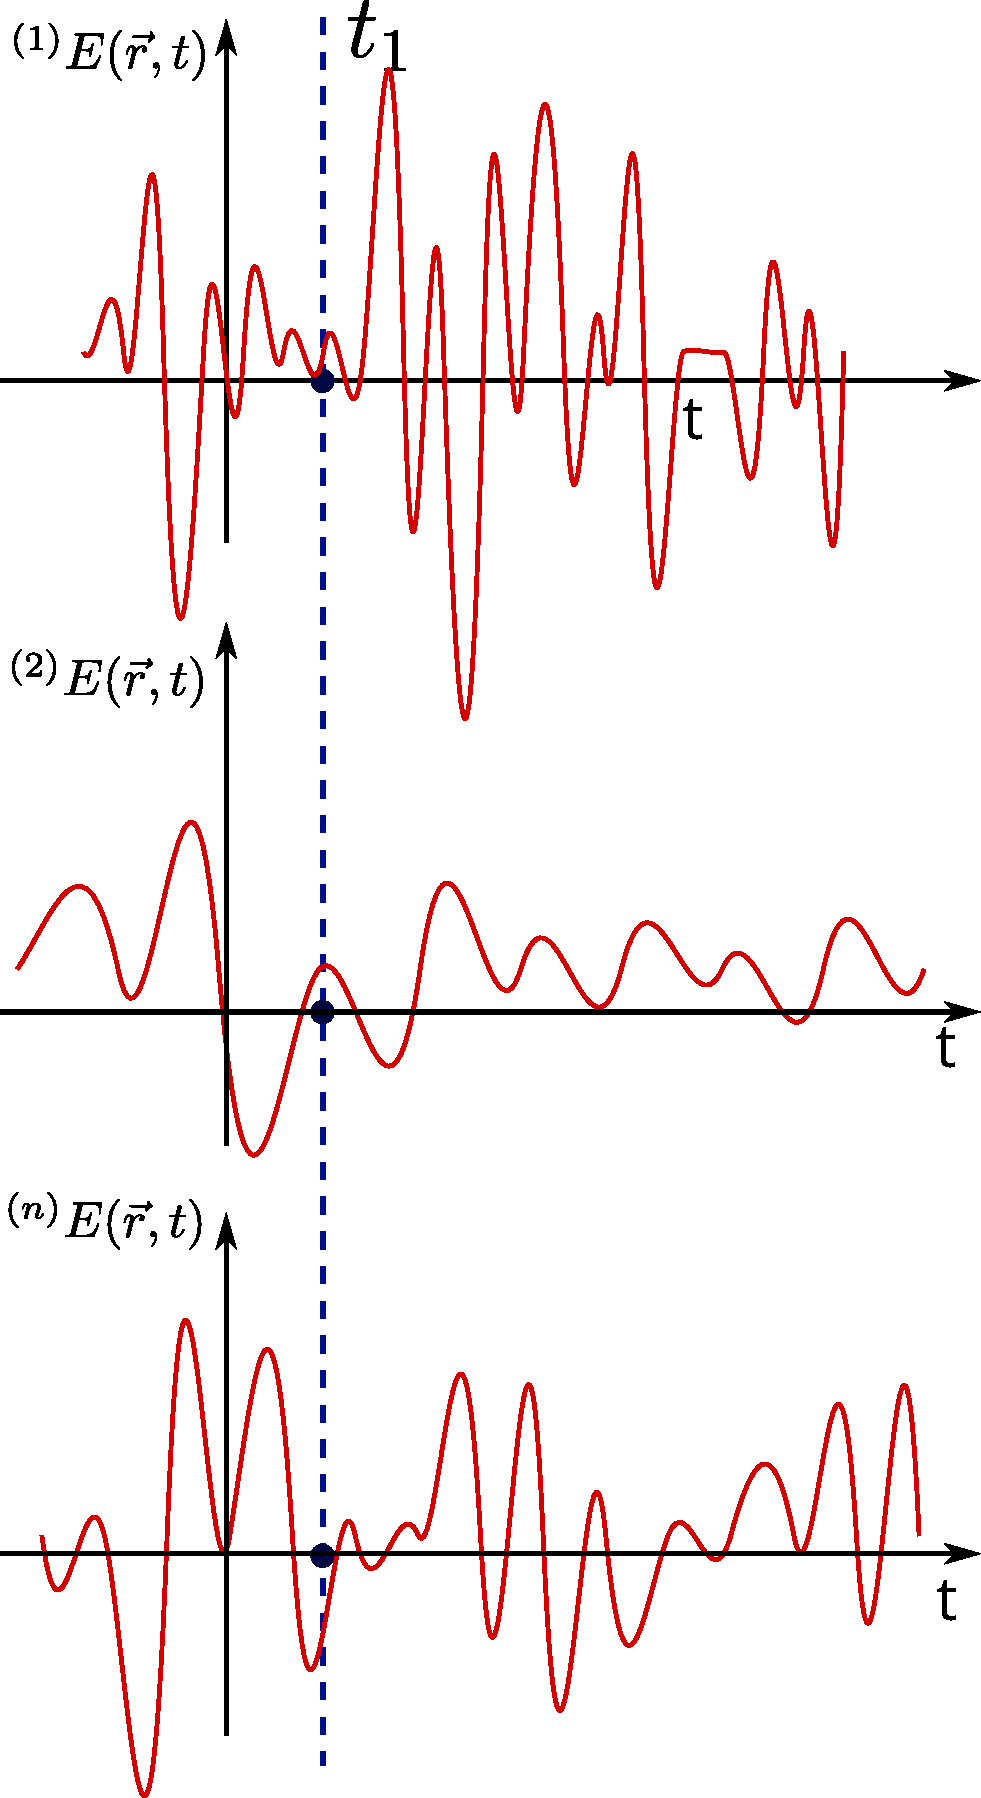
\includegraphics[width=0.4\linewidth]{Capitulo 2/Figuras/RandomVar}
		\caption{Representación de $E(\vec{r},t)$ como una variable aleatoria.}
		\label{fig:randomvar}
	\end{figure}

	En la Figura~\ref{fig:randomvar} observamos una componente del campo eléctrico, representada por $E(\vec{r},t)$, vista a través de varias observaciones o realizaciones. Comportándose como una variable aleatoria, en cada realización tiene un comportamiento distinto en el tiempo en un punto $\vec{r}$; en general, aquí hemos indexado $^{(i)}E(\vec{r},t)$ con enteros, pero en general podría haber un conjunto no numerable de estados posibles para el campo eléctrico. Si observamos la Figura~\ref{fig:randomvar} hay dos puntos temporales, $t,t'$, en los que aislamos partes de estas oscilaciones aleatorias; podríamos preguntar cuán correlacionadas están estas oscilaciones a través de las realizaciones a lo largo del intervalo $t'-t$, o dicho de otro modo, cuán \textit{coherentes} son las oscilaciones a través de las realizaciones.

	Hablamos de coherencia cuando queremos analizar la correlación de la radiación electromagnética entre puntos del espaciotiempo. Si tenemos dos fuentes que emiten un campo eléctrico (por el momento entendido como escalar), su función de coherencia viene dada por

	\begin{equation}
		\Gamma(\vec{r},\vec{r}';t,t') = E \left\{ \mathcal{E} (\vec{r},t) \mathcal{E}^*(\vec{r}',t') \right\},
	\end{equation}

	donde estamos calculando el promedio de ensamble de las componentes $\mathcal{E}$, que son números complejos como ya se discutió en estos apuntes. Si tomamos $\vec{r}=\vec{r}'$ obtenemos lo que se conoce como la \textit{función de coherencia mutua}

	\begin{equation}
		\Gamma(\vec{r}';t,t') = E \left\{ \mathcal{E}(\vec{r}',t) \mathcal{E}^*(\vec{r}',t') \right\}.
	\end{equation}

	Podemos ir aún más lejos incluyendo el concepto de \textit{estacionariedad estadística}, pero hay que tener cuidado pues existen varios tipos. Formalmente, un proceso estocástico $\{X_t\}$ se considera estacionario cuando sus propiedades estadísticas son invariantes bajo traslaciones temporales. Esta condición se manifiesta en distintos grados:

	\begin{enumerate}
		\item \textbf{Estacionariedad estricta (fuerte)}: la forma más exigente de estacionariedad requiere que todas las distribuciones de probabilidad conjuntas sean invariantes en el tiempo:

		\begin{equation}
			F_X(x_{t_1+\tau}, \ldots, x_{t_k+\tau}) = F_X(x_{t_1}, \ldots, x_{t_k}) \quad \forall \tau, k, t_i,
		\end{equation}
		donde $F_X$ es la función de distribución conjunta. Esto implica que:
		\begin{itemize}
			\item todos los momentos (media, varianza, asimetría, etc.) son constantes;
			\item las distribuciones marginales son idénticas en cualquier instante;
			\item es una condición suficiente pero no necesaria para los modelos ARMA.
		\end{itemize}

		\item \textbf{Estacionariedad débil (de segundo orden)}: más práctica en las aplicaciones, solo requiere la invariancia de los dos primeros momentos:
		\begin{equation}
			\begin{cases}
				\mathbb{E}[X_t] = \mu \quad (\text{constante}) \quad \forall t \\
				\text{Var}(X_t) = \sigma^2 \quad (\text{constante}) \quad \forall t \\
				\text{Cov}(X_t, X_{t+h}) = \gamma(h) \quad (\text{depende solo de } h, \text{ no de } t)
			\end{cases}
		\end{equation}
		Esta es la definición usada en la mayoría de los modelos econométricos (ARIMA, GARCH) y en el análisis espectral de Wiener-Khinchin (que usaremos más adelante).

		\item \textbf{Estacionariedad de tendencia (estacionariedad determinista)}: un proceso no estacionario que puede volverse estacionario removiendo componentes deterministas:
		\begin{equation}
			X_t = \alpha + \beta t + \epsilon_t,
		\end{equation}
		donde $\epsilon_t$ es estacionario. La no estacionariedad aquí proviene exclusivamente de la tendencia temporal $\beta t$.
	\end{enumerate}

	Usaremos una hipótesis de estacionariedad fuerte (aunque a menudo basta con la estacionariedad débil). En este espíritu, si $\tau = t-t'$ tenemos

	\begin{equation}
		\Gamma(\vec{r}',t,t') = \Gamma(\vec{r}',t-t') = \Gamma(\vec{r}',\tau).
	\end{equation}

	Como podemos ver, la coherencia mutua en un punto $\vec{r}'$ bajo una hipótesis de estacionariedad da lugar a una dependencia explícita en la diferencia temporal $\tau$ dentro del promedio de ensamble.

	Vale la pena preguntarse: ¿cuán necesario es analizar el promedio de ensamble; por qué no tomar el promedio temporal? Responder esto es \textit{muy complicado}, pues toca el problema de la \textit{ergodicidad}. La ergodicidad, en el sentido de la teoría ergódica, requiere que un sistema dinámico satisfaga que los promedios temporales coincidan con los promedios espaciales para casi toda condición inicial. Su demostración rigurosa es altamente no trivial, hasta el punto de que los problemas para los cuales la ergodicidad se ha demostrado con rigor matemático son pocos.

	Desde un punto de vista fenomenológico asumiremos, de aquí en adelante, una \textit{hipótesis ergódica} en la cual la radiación electromagnética tiene un carácter estacionario y ergódico. Bajo estas condiciones la función de coherencia mutua coincide con el promedio temporal

	\begin{equation}
		\Gamma(\vec{r}';t,t') = \int_{\mathbb{R}} \mathcal{E}(\vec{r}',t') \mathcal{E}^*(\vec{r}',t-t')\,dt'.
	\end{equation}

	La función de coherencia mutua tiene varias propiedades, algunas de las cuales son:

	\begin{itemize}
		\item[a)] $\Gamma(\vec{r}',0) \geq 0$. Esto se sigue de la definición, pues $\Gamma(\vec{r}',0) = \braket{|\mathcal{E}(\vec{r}')|^2}$, es decir, corresponde a la intensidad del campo eléctrico y solo puede anularse cuando trivialmente el campo es nulo en todo instante.

		\item[b)] $\Gamma(\vec{r}',-\tau) = \Gamma^*(\vec{r}',\tau)$. Esto se conoce como la \textit{propiedad hermítica} de la función de coherencia mutua, y se sigue del hecho de que $\mathcal{E}(\vec{r}',t)$ es estacionario, lo cual permite traslaciones temporales arbitrarias desde el origen. En este espíritu,

		\begin{align}
			& \Gamma(\vec{r}',\tau) = \braket{\mathcal{E}(\vec{r}')\mathcal{E}^*(\vec{r}',t + \tau)} = \braket{\mathcal{E}(\vec{r}',t-\tau)\mathcal{E}^*(\vec{r}')} = \Gamma^*(\vec{r}',-\tau).
		\end{align}

		\item[c)] $|\Gamma(\vec{r}',\tau)| \leq \Gamma(\vec{r}',0)$. Esta propiedad se sigue de la \textit{desigualdad de Cauchy-Schwarz}

		\begin{equation}
			|\Gamma(\vec{r}',\tau)|^2 = | \braket{\mathcal{E}(\vec{r}')\mathcal{E}^*(\vec{r}',t+\tau)} |^2 \leq  \braket{\mathcal{E}(\vec{r}',t)\mathcal{E}^*(\vec{r}',t)} \braket{\mathcal{E}(\vec{r}',t+\tau)\mathcal{E}^*(\vec{r}',t+\tau)} = \Gamma^2(\vec{r}',0),
		\end{equation}

		lo cual implica que $|\Gamma(\vec{r}',\tau)|$ jamás puede exceder su valor inicial $\Gamma(\vec{r}',0)$. (Esta propiedad es, recordemos, exclusiva de la función de coherencia mutua; cuando consideremos la coherencia entre dos fuentes veremos que no se cumple, sino que, por el contrario, aumentará.)

		\item[d)] $\Gamma(\vec{r}',\tau)$ es no negativa. Podemos ver esto a partir de la definición mediante la siguiente desigualdad, bastante obvia,

		\begin{equation}
			\left\langle \left| \int_{T_1}^{T_2} f(t)\mathcal{E}(t)\,dt \right|^2\right\rangle \geq 0,
		\end{equation}
		donde $f(t)$ es una función arbitraria y $T_1,T_2$ son instantes arbitrarios. De este modo obtenemos la desigualdad

		\begin{equation}
			\int_{T_1}^{T_2}\int_{T_1}^{T_2} f^*(\vec{r}',t)f(\vec{r}',t')\Gamma(\vec{r}',t'-t)\,dt\,dt' \geq 0.
		\end{equation}

		\item[e)] Si el campo eléctrico es aleatorio, estacionario y diferenciable, entonces podemos hallar una velocidad $\xi (\vec{r}',t) = \dot{\mathcal{E}}(\vec{r}',t)$, que es estacionaria, aleatoria y de valor medio nulo, y cuya función de coherencia mutua es

		\begin{equation}
			\Gamma_\xi(\vec{r}',\tau) = - \ddot{\Gamma}_\mathcal{E}(\vec{r}',\tau).
		\end{equation}

		\item[f)] $\Gamma(\vec{r}',\tau)$ es continua. Esto se cumple incluso cuando hay discontinuidades de salto.
	\end{itemize}

	Finalmente, vale la pena mencionar que existe una cantidad conocida como el grado complejo de coherencia, dada por

	\begin{equation}
		\gamma (\vec{r}',\tau) = \frac{\Gamma(\vec{r}',\tau)}{\Gamma(\vec{r}',0)},
	\end{equation}

	y a partir de la desigualdad de Cauchy-Schwarz tenemos $0 \leq |\gamma(\vec{r}',\tau)| \leq 1$.

	\subsection{Manifestaciones de la coherencia: el teorema de Wiener-Khinchin}

		La función de coherencia mutua y la densidad espectral de potencia son dos caras de la misma moneda en el estudio de la luz y las señales ondulatorias. La coherencia mutua describe cómo se correlacionan las fluctuaciones de un campo luminoso en el espacio y en el tiempo, actuando como un mapa que revela hasta qué punto las variaciones en un punto del espacio están sincronizadas con las de otro, incluso con cierto retardo temporal. La densidad espectral de potencia, a su vez, descompone la energía de la señal en sus componentes de frecuencia, mostrando qué tonos o colores —en el caso de la luz— dominan su comportamiento. La relación íntima entre ambos conceptos radica en que, mediante transformaciones matemáticas, es posible convertir la información detallada sobre las correlaciones espaciotemporales capturada por la coherencia mutua en una descripción precisa de cómo se distribuye la energía en el dominio de la frecuencia, y viceversa. Este vínculo permite saltar entre perspectivas complementarias: analizar patrones de interferencia en un interferómetro o identificar firmas espectrales en un material, todo a partir de los mismos principios fundamentales.

		Vamos a encontrar uno de los teoremas más importantes de la teoría de la coherencia, el \textit{teorema de Wiener-Khinchin}. Nótese que las señales aleatorias estacionarias no tienen transformada de Fourier; por ello podemos definir las siguientes señales aleatorias truncadas del campo eléctrico

		\begin{equation}\label{eq:NearlyWiener}
			^\omega \mathcal{E}_T (\vec{r},t) = \left\{
			\begin{matrix}
				^\omega\mathcal{E}(\vec{r},t) & -\frac{T}{2}\leq t \leq \frac{T}{2}\\
				0 & \text{en otro caso}
			\end{matrix} \right.
		\end{equation}

		y definimos la potencia espectral para una realización $\omega$ como la magnitud al cuadrado de las transformadas de Fourier de los campos eléctricos \eqref{eq:NearlyWiener}, es decir,

		\begin{equation}\label{eq:SpecWT}
			^\omega S_T (\vec{r},\nu) = \left| \int_\mathbb{R} ^\omega \mathcal{E}_T(\vec{r},t)e^{i2\pi\nu t}dt \right|^2 = \left| \int_{-T/2}^{T/2}\;^\omega \mathcal{E}(\vec{r},t)e^{i2\pi\nu t}dt \right|^2,
		\end{equation}

		y la \textit{densidad espectral de potencia del evento} $\omega$ la calculamos como

		\begin{equation}\label{eq:SpecW}
			\lim_{T \to \infty} \frac{^\omega S_T(\vec{r},\nu)}{T} = {}^\omega S(\vec{r},\nu).
		\end{equation}

		Puesto que ya poseemos una herramienta para estudiar, en cada evento o realización, la densidad espectral de potencia, entonces, mediante su promedio de ensamble, podemos hallar la densidad total, es decir,

		\begin{equation}
			S(\vec{r},\nu) = E\left\{^\omega S(\vec{r},\nu)\right\},
		\end{equation}

		introduciendo las ecuaciones \eqref{eq:SpecWT} y \eqref{eq:SpecW} tenemos entonces

		\begin{align}
			& S(\vec{r},\nu) = E\left\{ \lim_{T \to \infty} \left| \frac{1}{T} \int_{-T/2}^{T/2}\;^\omega \mathcal{E}(\vec{r},t)e^{i2\pi\nu t}dt \right|^2 \right\},\\
			& S(\vec{r},\nu) = \lim_{T \to \infty} \frac{1}{T}  \int_{-T/2}^{T/2}\int_{-T/2}^{T/2} E \left\{ \mathcal{E}(\vec{r},t)\mathcal{E}^*(\vec{r}',t') \right\} e^{i2\pi\nu(t-t')}dt\,dt',\\
			& S(\vec{r},\nu) = \int_{\mathbb{R}}\Gamma(\vec{r},\vec{r}';\tau)e^{i2\pi\nu \tau}d\tau,
		\end{align}

		\begin{equation}\label{eq:WienerKhinchin}
			\boxed{S(\vec{r},\nu) = \mathcal{F}\left\{ \Gamma(\vec{r},\vec{r}',\tau) \right\}}.
		\end{equation}

		El resultado \eqref{eq:WienerKhinchin} se lee: la transformada de Fourier de la función de coherencia corresponde a la densidad espectral de potencia, y se conoce como el teorema de Wiener-Khinchin. Su uso es fundamental, pues nos dice que mediante métodos como la espectrometría podemos hallar la función de coherencia de cualquier fenómeno; podemos incluso ir más lejos, ya que este resultado en realidad se desprende de algo más general —la función de correlación—, lo que significa que todo fenómeno estocástico tiene un espectro asociado, y a partir de las mediciones o estimaciones de ese espectro podemos calcular las correlaciones del sistema.

		Si hacemos una observación simple, el rango óptico de la radiación —el visible— es una banda de frecuencias muy bajas respecto de todo el espectro; el visible va aproximadamente de $400$~nm a $700$~nm, y podemos decir que toda la óptica es de \textit{banda angosta}. Esto obedece la desigualdad

		\begin{equation}
			\frac{\triangle \nu}{\nu} \ll 1,
		\end{equation}

		y, en este régimen de banda angosta, la función de coherencia toma la forma

		\begin{equation}
			\Gamma(\vec{r};\tau) = \tilde{\Gamma}(\vec{r})e^{i2\pi \tilde{\nu}\tau},
		\end{equation}

		lo cual podemos representar gráficamente como se muestra en la Figura~\ref{fig:narrow}, donde se puede ver el comportamiento de la función de coherencia en el régimen de banda angosta.\footnote{Suele encontrarse en la literatura un término parecido pero no igual al de banda angosta, conocido como la condición de cuasimonocromaticidad, escrita como $\frac{\triangle \lambda}{\lambda} \ll 1$; pero esto acota la longitud de onda para que sea lo más monocromática posible, mientras que la condición de banda angosta admite varias frecuencias, siempre que sean angostas respecto de todo el espectro de frecuencias.} Allí se observa una envolvente (lo observable) que envuelve todas las frecuencias fundamentales.

		\begin{figure}[htbp]
			\centering
			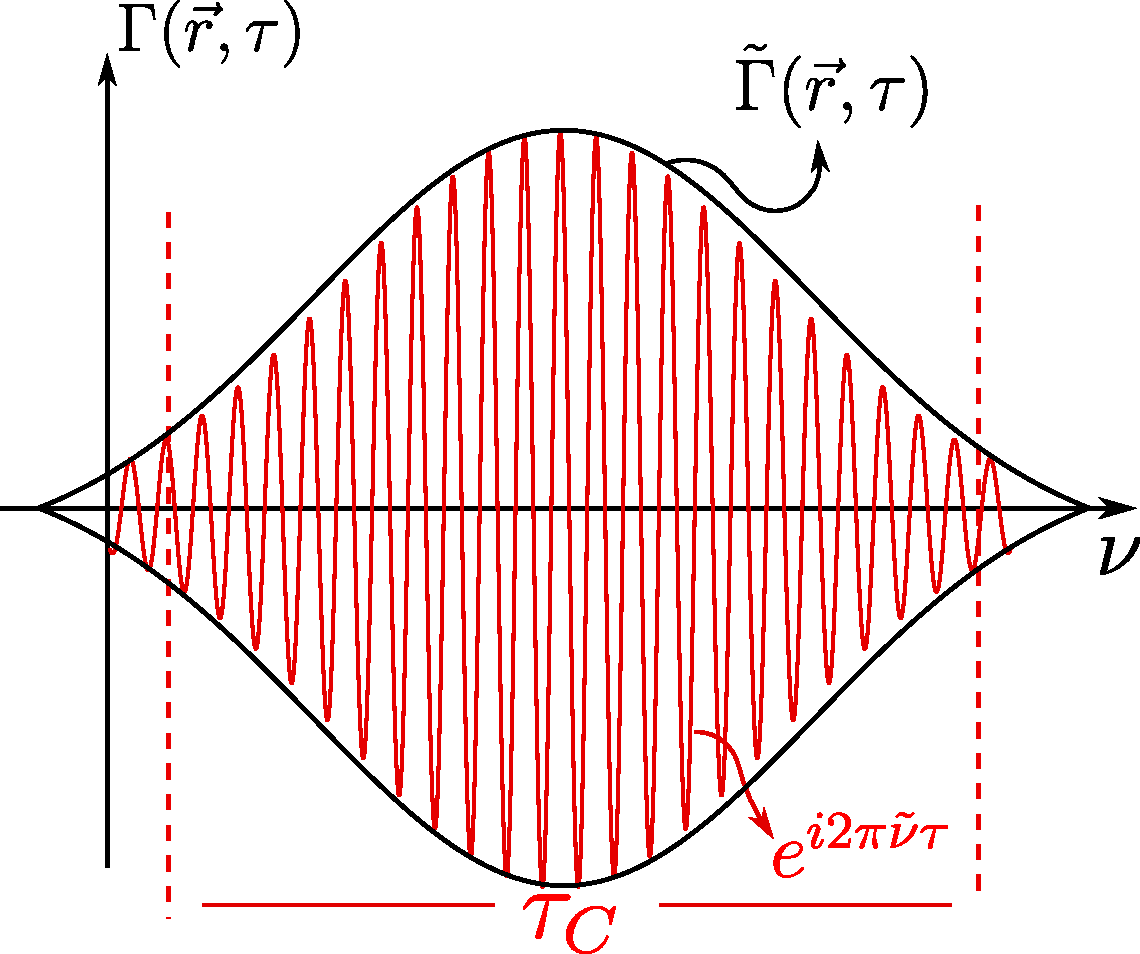
\includegraphics[width=0.7\linewidth]{Capitulo 2/Figuras/Estrecho}
			\caption{Representación gráfica de la función de coherencia de banda angosta. En negro se muestra la envolvente $\tilde{\Gamma}(\vec{r},\tau)$, y en rojo las oscilaciones $e^{i2\pi\tilde{\nu}\tau}$. Estas oscilaciones están confinadas dentro de algo conocido como el tiempo de coherencia $\tau_C$, que veremos más adelante.}
			\label{fig:narrow}
		\end{figure}

	\subsection{Ecuación de onda de la coherencia}

		Salgamos un poco de la zona de confort y comprendamos cómo se propagan las correlaciones a través del espacio y del tiempo. Sea $\mathcal{E}^{(r)}(\vec{r},t)$ alguna componente \textit{real} del campo eléctrico, vista como una señal aleatoria. Como es bien sabido a partir de la teoría electromagnética clásica, obedece las ecuaciones de Maxwell y por tanto tiene asociada una ecuación de onda, a saber

		\begin{equation}
			\nabla^2 \mathcal{E}^{(r)}(\vec{r},t) = \frac{1}{C^2}\frac{\partial^2 \mathcal{E}^{(r)}(\vec{r},t)}{\partial t^2},
		\end{equation}

		donde $C$ es la velocidad de la luz en el vacío. También tenemos, por análisis de Fourier,

		\begin{equation}\label{eq:EandFourier}
			\mathcal{E}(\vec{r},t) = \int_0^{\infty} \tilde{\mathcal{E}}(\vec{r},\nu) e^{-i2\pi\nu t}d\nu .
		\end{equation}

		Y si aplicamos el operador d'alembertiano $\square = \nabla^2 - \frac{1}{C^2}\frac{\partial^2}{\partial t^2}$ a la ecuación \eqref{eq:EandFourier}, encontramos que $\tilde{\mathcal{E}}(\vec{r},\nu)$ tiene la forma de una ecuación de tipo Helmholtz, es decir,

		\begin{equation}
			\nabla^2 \mathcal{E}(\vec{r},t) - \frac{1}{C^2}\frac{\partial^2 \mathcal{E}(\vec{r},t)}{\partial t^2} = \int_0^{\infty} \left[ \nabla^2 \tilde{\mathcal{E}}(\vec{r},\nu) + k^2 \tilde{\mathcal{E}}(\vec{r},\nu) \right]e^{-i2\pi\nu t}d\nu,
		\end{equation}

		lo que nos lleva al hecho de que el campo eléctrico, como señal analítica y compleja, también obedece una ecuación de tipo ondulatorio

		\begin{equation}
			\nabla^2 \mathcal{E}(\vec{r},t) = \frac{1}{C^2}\frac{\partial^2 \mathcal{E}(\vec{r},t)}{\partial t^2}.
		\end{equation}

		Tomando el complejo conjugado de la ecuación anterior tenemos

		\begin{equation}\label{eq:NearlyWaveForE}
			\nabla^2 \mathcal{E}^*(\vec{r},t) = \frac{1}{C^2}\frac{\partial^2 \mathcal{E}^*(\vec{r},t)}{\partial t^2}.
		\end{equation}

		Si multiplicamos ambos lados de la ecuación \eqref{eq:NearlyWaveForE} por $\mathcal{E}(\vec{r}',t')$, y dado que hemos tomado el d'alembertiano respecto de las variables sin prima, usando algunas reglas de signos tenemos

		\begin{equation}\label{eq:NoAvg}
			\nabla^2 \left[ \mathcal{E}^*(\vec{r},t)\mathcal{E}(\vec{r}',t') \right] =  \frac{1}{C^2} \frac{\partial^2}{\partial t^2}\left[ \mathcal{E}^*(\vec{r},t)\mathcal{E}(\vec{r}',t') \right].
		\end{equation}

		Tomando el promedio de ensamble de la ecuación \eqref{eq:NoAvg} sobre todas las realizaciones del campo, esta ecuación de onda se convierte en

		\begin{equation}\label{eq:coherenceWave1}
			\nabla^2 \Gamma(\vec{r},\vec{r}';t,t') = \frac{1}{C^2}\frac{\partial^2}{\partial t^2} \Gamma(\vec{r},\vec{r}';t,t'),
		\end{equation}

		y, de manera análoga, usando $\square' = \nabla'^2 - \frac{1}{C^2}\frac{\partial^2}{\partial t'^2}$ tenemos otra ecuación de onda dada por

		\begin{equation}\label{eq:coherenceWave2}
			\nabla'^2 \Gamma(\vec{r},\vec{r}';t,t') = \frac{1}{C^2}\frac{\partial^2}{\partial t'^2} \Gamma(\vec{r},\vec{r}';t,t').
		\end{equation}

		Las ecuaciones \eqref{eq:coherenceWave1} y \eqref{eq:coherenceWave2} nos dicen directamente que las funciones de coherencia entre dos puntos del espaciotiempo evolucionan en el tiempo siguiendo una ecuación de tipo ondulatorio, por separado, respecto de cada par de coordenadas espaciotemporales —un resultado que es, sin duda, notable—. Podemos llevar este resultado aún más lejos y estudiar esta propagación en la siguiente sección.

	\subsection{Propagación de la coherencia y la dirección del tiempo: el teorema de van Cittert-Zernike}

		\begin{figure}[htbp]
			\centering
			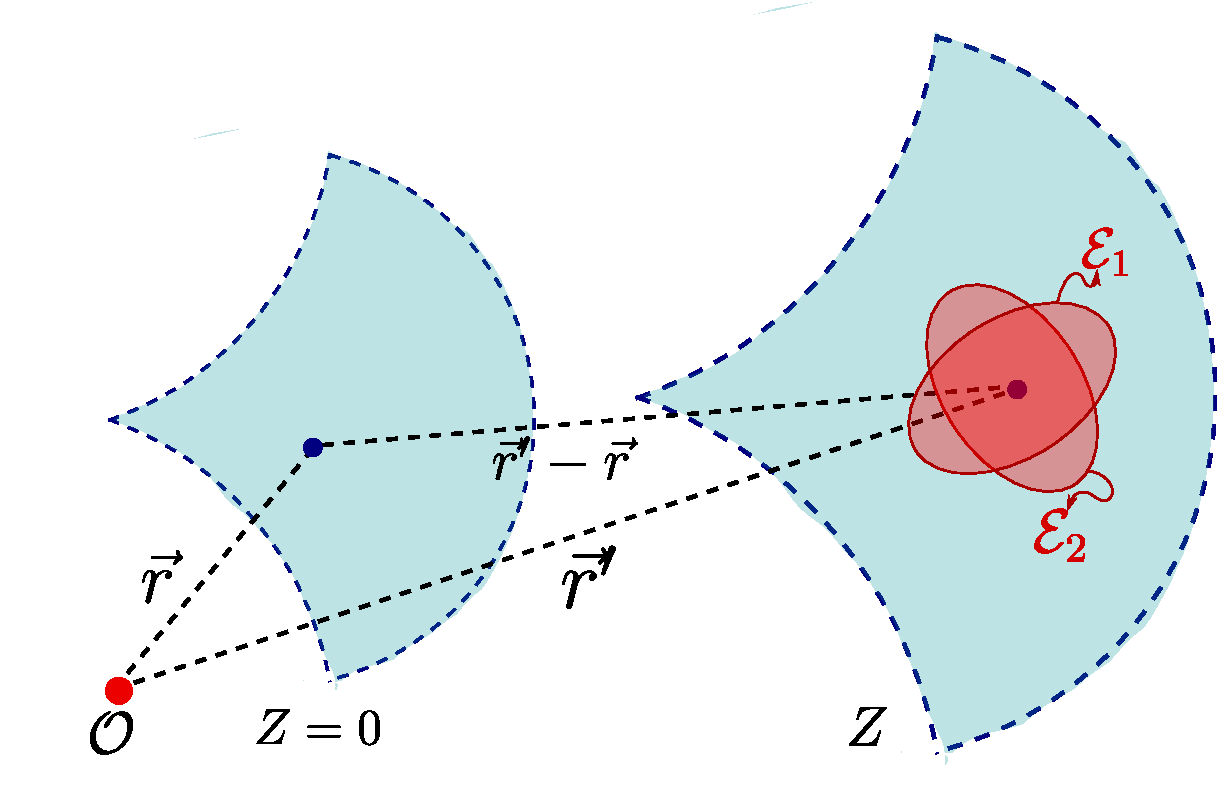
\includegraphics[width=0.8\linewidth]{Capitulo 2/Figuras/Propagation}
			\caption{Propagación del campo eléctrico desde un plano $Z=0$ hasta un plano $Z$, donde cada punto del frente de onda lleva su elipse de polarización media.}
			\label{fig:propagation}
		\end{figure}

		Como sabemos, el campo eléctrico obedece una ecuación de tipo ondulatorio y la orientación de los campos viene dada por la polarización del campo; a su vez, como vimos en el capítulo de difracción (véase la Sección~\ref{Sec:Diffraction}), a nivel clásico la luz se propaga fundamentalmente como ondas esféricas, tal como se ilustra en la Figura~\ref{fig:propagation}, y en cada punto del frente de onda las componentes del campo eléctrico oscilan aleatoriamente, pero dentro de la elipse de polarización media de su estado representativo. Matemáticamente podemos representar esta componente como

		\begin{equation}
			\mathcal{E}_z(\vec{r}_1,\nu) = \frac{i}{\lambda} \int_{\Sigma} \mathcal{E}_0 (\vec{r},\nu) \frac{e^{ik \|\vec{r}_1-\vec{r}\|}}{\|\vec{r}_1-\vec{r}\|}\cos(\hat{z}; \vec{r}_1-\vec{r})\,d\sigma .
		\end{equation}

		Usando la ecuación \eqref{eq:EandFourier} tenemos

		\begin{equation}
			\mathcal{E}_z(\vec{r}_1,t) = \frac{1}{i}\int_{\mathbb{R}^+} \frac{\nu}{V} \int_{\Sigma} \mathcal{E}_0(\vec{r},\nu)\frac{\cos\left(  \hat{z}; \vec{r}_1 - \vec{r} \right)}{\|\vec{r}_1 - \vec{r}\|} e^{i2\pi \nu \left( t + \frac{\|\vec{r}_1 - \vec{r}\|}{V} \right)} d\sigma\, d\nu,
		\end{equation}

		donde $V$ es la velocidad de propagación de la envolvente. Reescribiendo un poco más, tenemos

		\begin{equation}
			\mathcal{E}_z(\vec{r}_1,t) = \frac{1}{i} \int_{\Sigma} \frac{\cos\left( \hat{z}; \vec{r}_1-\vec{r} \right)}{\|\vec{r}_1 -\vec{r}\|} \int _{\mathbb{R}^+} \frac{\nu}{V} \mathcal{E}_0 (\vec{r},\nu)e^{i2\pi\nu \left(t + \frac{\|\vec{r}_1 - \vec{r}\|}{V}\right)}d\nu\, d\sigma,
		\end{equation}

		y, tomando la aproximación de banda angosta, tenemos

		\begin{equation}\label{eq:IntegralEz}
			\mathcal{E}_z(\vec{r}_1,t) = \frac{1}{i\tilde{\lambda}} \int_{\Sigma} \mathcal{E}_0 \left(\vec{r}, t +\frac{\|\vec{r}_1 - \vec{r}\|}{V}\right) \frac{\cos\left(\hat{z} ; \vec{r}_1 - \vec{r}\right)}{\|\vec{r}_1-\vec{r}\|} d\sigma .
		\end{equation}

		Podemos visualizar gráficamente cómo pretendemos propagar en la Figura~\ref{fig:propagation2}, donde observamos que estamos partiendo de la función de coherencia entre dos puntos $\vec{r},\vec{r}'$ en los instantes $t,t'$, respectivamente, y llevándola hasta una función de coherencia en los puntos $\vec{r}_1,\vec{r}_2$ en dos instantes $t_1,t_2$, respectivamente.

		\begin{figure}[htbp]
			\centering
			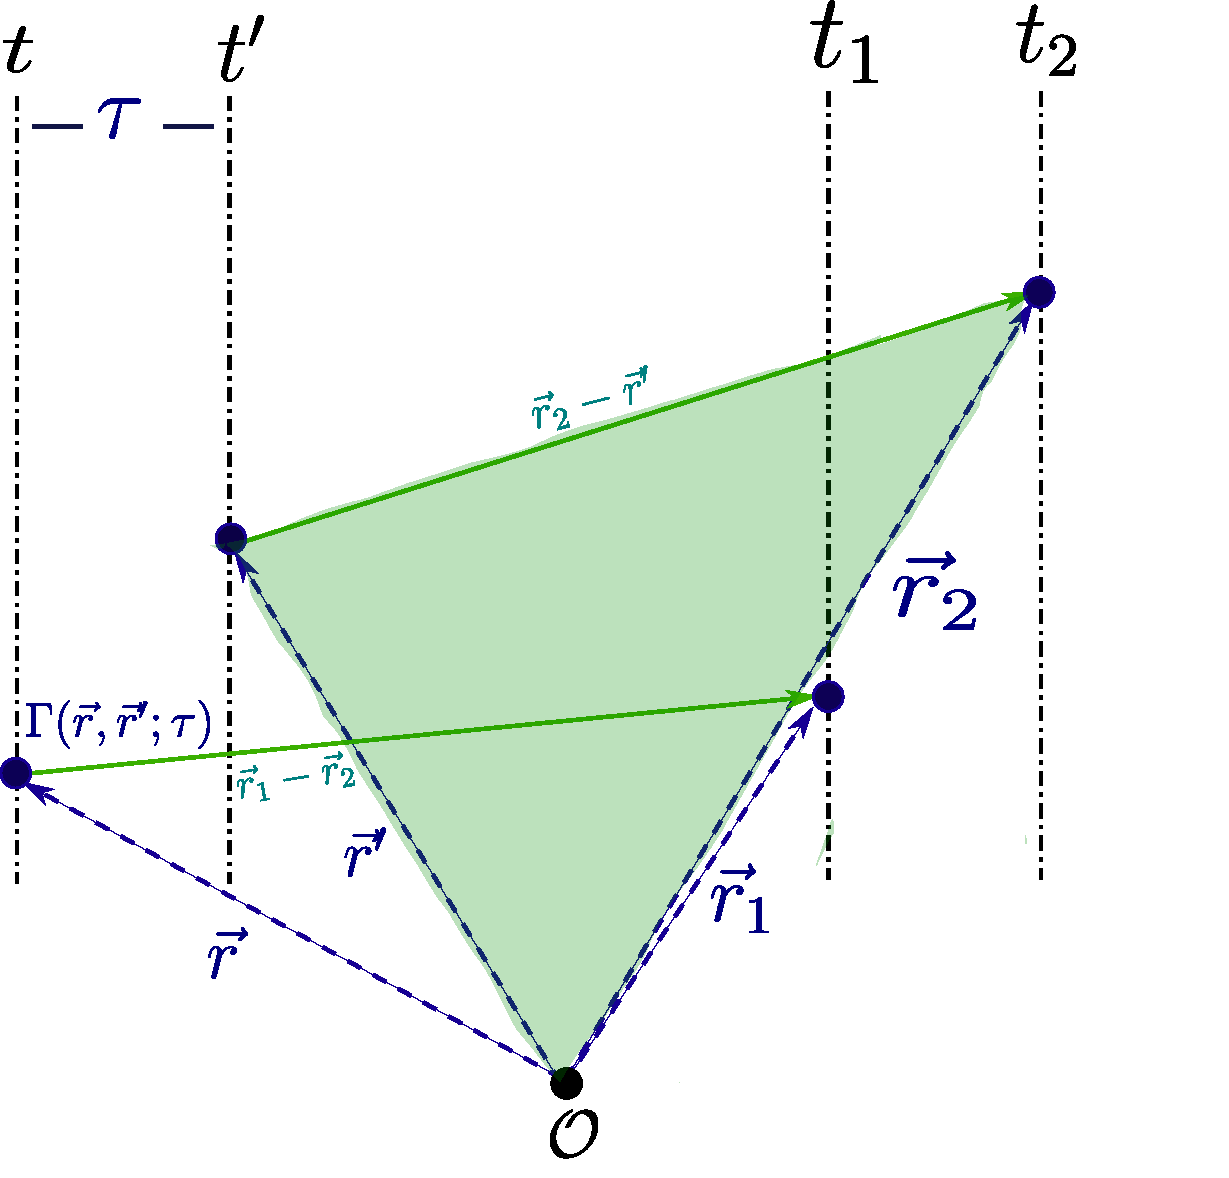
\includegraphics[width=0.8\linewidth]{Capitulo 2/Figuras/Propagation2}
			\caption{Propagación de la función de coherencia entre dos puntos $\vec{r},\vec{r}'$ en el plano inicial hasta la coherencia entre dos puntos $\vec{r}_1,\vec{r}_2$ en el plano de observación.}
			\label{fig:propagation2}
		\end{figure}

		Partiendo de la ecuación \eqref{eq:IntegralEz} podemos calcular la función de coherencia en su propagación como

		\begin{equation}
			\Gamma_z(\vec{r}_1,\vec{r}_2;\tau) = E \left\{ \mathcal{E}_z(\vec{r}_1,t) \mathcal{E}_z^*(\vec{r}_2,t-\tau) \right\},
		\end{equation}

		\begin{align}
			&\Gamma_z(\vec{r}_1,\vec{r}_2;\tau) = E\left\{\frac{1}{i\tilde{\lambda}} \int_{\Sigma} \mathcal{E}_0 \left(\vec{r},t + \frac{\|\vec{r}_1 - \vec{r}\|}{V}\right) \frac{\cos\left(\hat{z};\vec{r}_1-\vec{r}\right)}{\|\vec{r}_1-\vec{r}\|}d\sigma \right. \\
			& \left. \cdot \frac{1}{-i\tilde{\lambda}} \int_{\Sigma'} \mathcal{E}_0^* \left(\vec{r}',t - \tau + \frac{\|\vec{r}_2 - \vec{r}'\|}{V}\right) \frac{\cos\left(\hat{z};\vec{r}_2-\vec{r}'\right)}{\|\vec{r}_2-\vec{r}'\|}d\sigma'  \right\},
		\end{align}

		\begin{align}
			& \Gamma_z(\vec{r}_1,\vec{r}_2;\tau) = \frac{1}{\tilde{\lambda}^2} \int_{\Sigma}\int_{\Sigma'} E \left\{ \mathcal{E}_0\left(\vec{r}, t + \frac{\|\vec{r}_1 - \vec{r}\|}{V}\right) \mathcal{E}_0^* \left(\vec{r}', t-\tau + \frac{\|\vec{r}_2 - \vec{r}'\|}{V}\right) \right\}\frac{\cos \left(\hat{z};\vec{r}_1-\vec{r}\right) \cos\left(\hat{z}; \vec{r}_2 - \vec{r}' \right) }{\|\vec{r}_2-\vec{r}'\|\cdot \|\vec{r}_1 - \vec{r}\|} d\sigma\, d\sigma',
		\end{align}

		\begin{equation}\label{eq:IntGamma}
			\Gamma_z (\vec{r}_1,\vec{r}_2;\tau) = \frac{1}{\tilde{\lambda}^2}\int_{\Sigma}\int_{\Sigma'} \Gamma_0 \left(\vec{r},\vec{r}';\tau + \frac{\|\vec{r}_1 - \vec{r}\| + \|\vec{r}_2 - \vec{r}'\|}{V}\right) \frac{\cos \left(\hat{z};\vec{r}_1-\vec{r}\right) \cos\left(\hat{z}; \vec{r}_2 - \vec{r}' \right) }{\|\vec{r}_2-\vec{r}'\|\cdot \|\vec{r}_1 - \vec{r}\|} d\sigma\, d\sigma'
		\end{equation}

		\begin{figure}[htbp]
			\centering
			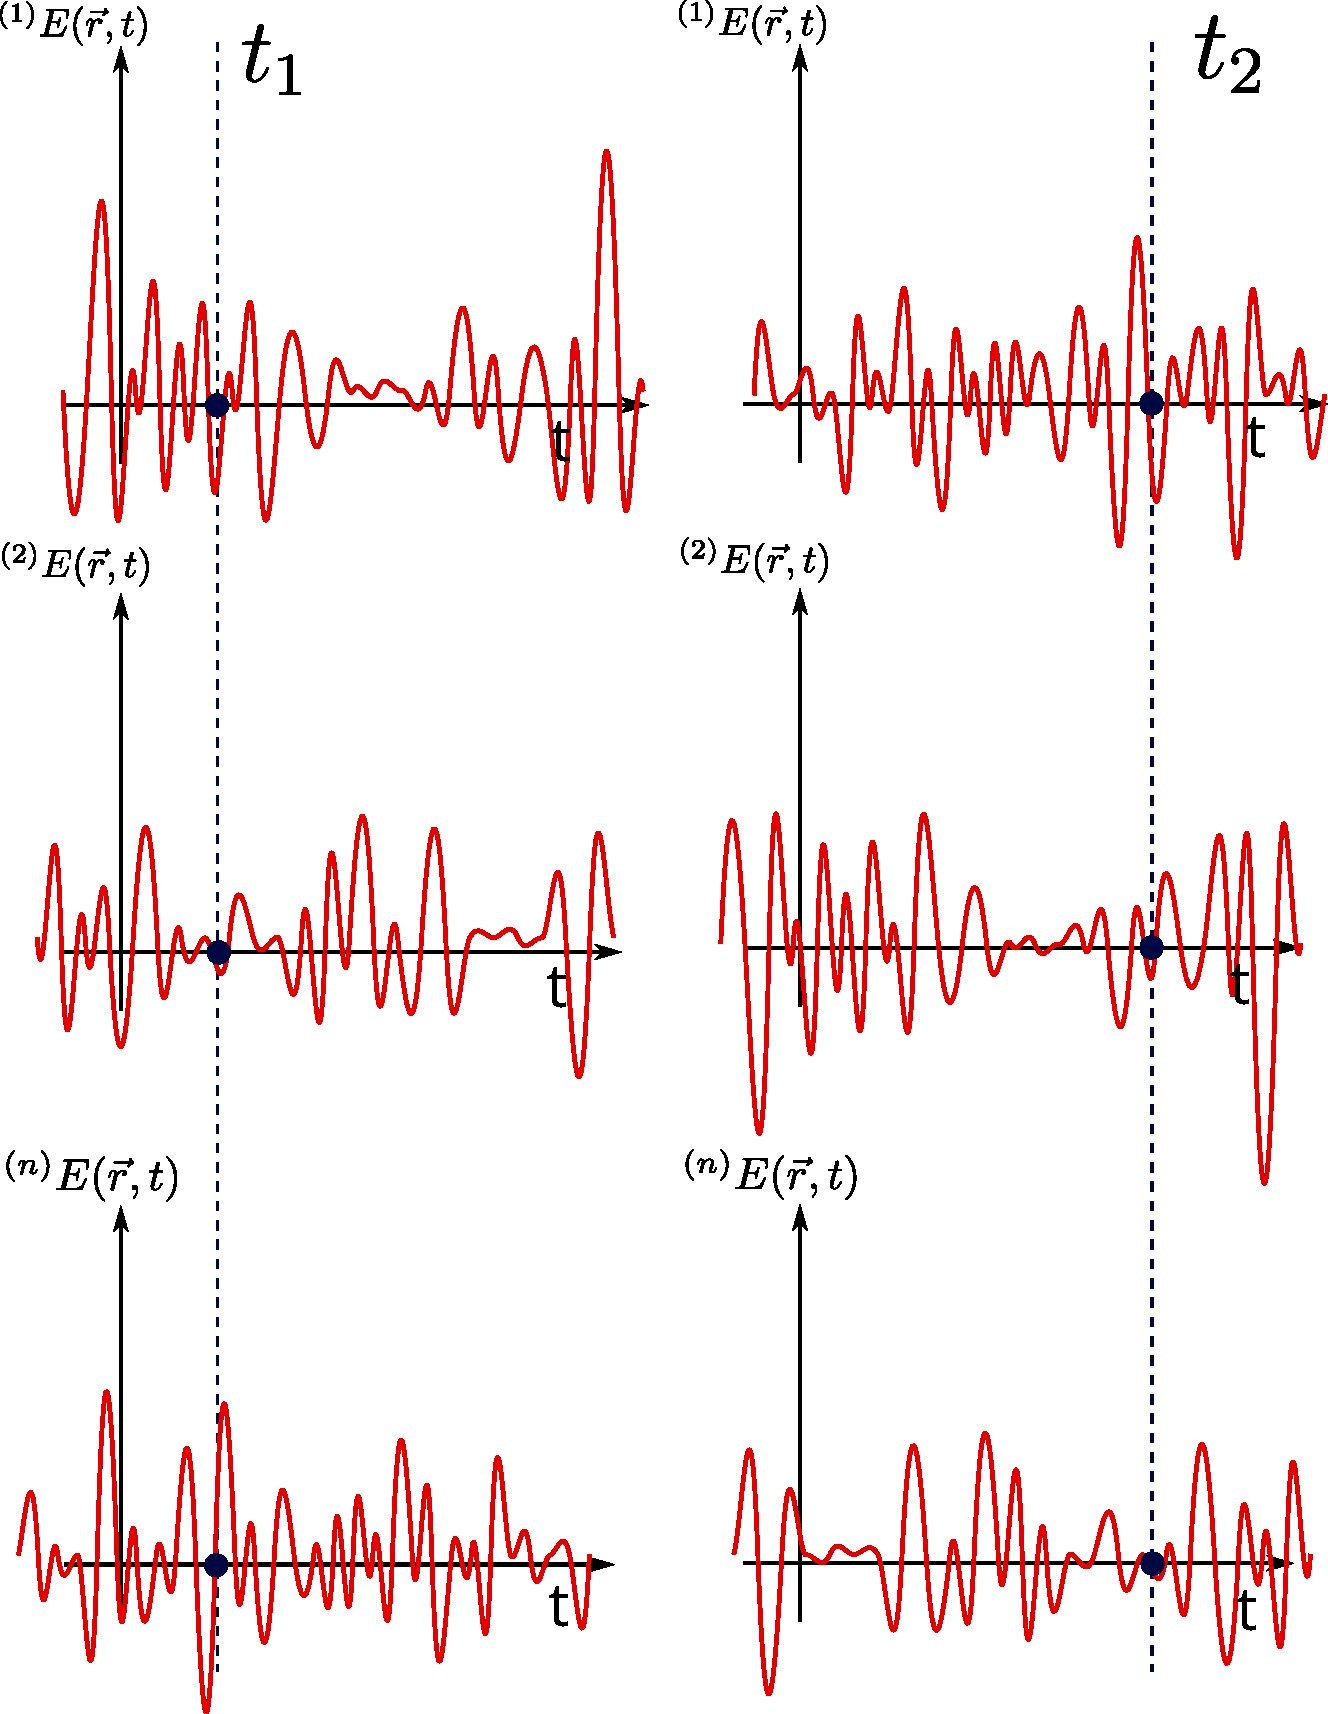
\includegraphics[width=0.6\linewidth]{Capitulo 2/Figuras/Random2}
			\caption{Evolución de las realizaciones al propagar el campo eléctrico.}
			\label{fig:random2}
		\end{figure}

		La propagación de las oscilaciones aleatorias a través de $n$ realizaciones puede visualizarse en la Figura~\ref{fig:random2}.

		Vamos a imponer la siguiente condición sobre la función de coherencia

		\begin{equation}
			\Gamma(\vec{r},\vec{r}';\tau) = \Gamma(\vec{r}';\tau) \delta(\vec{r}-\vec{r}'),
		\end{equation}

		lo cual, en pocas palabras, significa que, espacialmente hablando, la distribución que representa la función de coherencia está localizada en un punto y ponderada por la coherencia mutua en el punto $\vec{r}'$. Imponiendo esto en la ecuación \eqref{eq:IntGamma} tenemos

		\begin{equation}
			\Gamma_z\left(\vec{r}_1,\vec{r}_2;\tau\right) = \frac{1}{\tilde{\lambda}^2}\int_{\Sigma}\Gamma_0 \left( \vec{r}; \tau + \frac{\|\vec{r}-\vec{r}_1\| - \|\vec{r} -\vec{r}_2\| }{V} \right)\frac{\cos \left(\hat{z};\vec{r}_1-\vec{r}\right) \cos\left(\hat{z}; \vec{r}_2 - \vec{r} \right) }{\|\vec{r}_2-\vec{r}\|\cdot \|\vec{r}_1 - \vec{r}\|} d\sigma .
		\end{equation}

		En la naturaleza no siempre tendremos fuentes de banda angosta; sin embargo, podemos recurrir a otro argumento, a saber, que la mayoría de los instrumentos no tienen un rango infinito o amplio sino uno corto —o, dicho de otro modo, los instrumentos de medición miden una porción angosta del espectro—. Por tanto, incluyendo la condición de banda angosta tenemos

		\begin{equation}
			\Gamma_z(\vec{r}_1,\vec{r}_2)e^{i2\pi\tilde{\nu}\tau} = \frac{1}{\tilde{\lambda}^2} \int_{\Sigma} \Gamma_0(\vec{r})e^{i2\pi\tilde{\nu} \left( \tau + \frac{\|\vec{r} - \vec{r}_1\| - \|\vec{r}-\vec{r}_2\|}{V} \right) } \frac{\cos \left(\hat{z};\vec{r}_1-\vec{r}\right) \cos\left(\hat{z}; \vec{r}_2 - \vec{r} \right) }{\|\vec{r}_2-\vec{r}\|\cdot \|\vec{r}_1 - \vec{r}\|} d\sigma .
		\end{equation}

		Dado el tiempo de coherencia definido por $\tau_C = \int_{\mathbb{R}^+}| \gamma(\vec{r},\tau) |^2 d\tau$, y si imponemos una condición de tiempos muy pequeños, menores que un tiempo de coherencia $\tau \ll \tau_C$, tenemos

		\begin{equation}
			\Gamma_z(\vec{r}_1,\vec{r}_2) = \frac{1}{\tilde{\lambda}^2}\int_{\Sigma}I_0(\vec{r})e^{i2\pi \left( \frac{\|\vec{r}-\vec{r}_1\| - \|\vec{r} - \vec{r}_2\|}{V/\tilde{\nu}} \right)} \frac{\cos \left(\hat{z};\vec{r}_1-\vec{r}\right) \cos\left(\hat{z}; \vec{r}_2 - \vec{r} \right) }{\|\vec{r}_2-\vec{r}\|\cdot \|\vec{r}_1 - \vec{r}\|} d\sigma .
		\end{equation}

		Tomando la aproximación de campo lejano podemos simplificar el problema como sigue

		\begin{equation}\label{eq:IntegralProx}
			\Gamma_z(\vec{r}_1,\vec{r}_2) = \frac{1}{\tilde{\lambda}^2 z^2} \int_{\Sigma} I_0(\vec{r}) e^{i2\pi \left( \frac{\|\vec{r}-\vec{r}_1\| - \|\vec{r} - \vec{r}_2\|}{V/\tilde{\nu}} \right)} d\sigma .
		\end{equation}

		Podemos ahora hacer una expansión en serie de Taylor, la misma realizada en el capítulo de difracción. En este espíritu los siguientes términos se convierten en

		\begin{align}
			& \|\vec{r} - \vec{r}_1\| = \left( z^2 + (x-x_1)^2 + (y-y_1)^2 \right)^{1/2} = z \left(1 + \frac{(x-x_1)^2 + (y-y_1)^2}{z^2}\right)^{1/2} \approx z + \frac{(x-x_1)^2 + (y-y_1)^2}{2z},\\
			& \|\vec{r}-\vec{r}_2\| \approx z + \frac{(x-x_2)^2 + (y-y_2)^2}{2z}.
		\end{align}

		Introduciendo esto en la integral \eqref{eq:IntegralProx} obtenemos

		\begin{equation}
			\Gamma_z (\vec{r}_1,\vec{r}_2) = \frac{1}{\tilde{\lambda}^2 z^2}\int_{\mathbb{R}^2}I_0(x,y)e^{-\frac{i2\pi}{\tilde{\lambda}z}\left(xx_1 + yy_1\right)}e^{\frac{i2\pi}{\tilde{\lambda} z}(xx_2 + yy_2)} e^{-\frac{i\pi}{\tilde{\lambda}z}(x_1^2 + y_1^2)}dx\,dy.
		\end{equation}

		Definamos los vectores $\vec{S}_1 = (x_1,y_1)$, $\vec{S}_2 = (x_2,y_2)$ y $\vec{S} = (x,y)$. Entonces

		\begin{equation}
			\Gamma_z(\vec{S}_1,\vec{S}_2) = \frac{e^{i \frac{\pi}{\tilde{\lambda}z} (\|\vec{S}_1\|^2 - \|\vec{S}_2\|^2)}}{\tilde{\lambda}^2 z^2} \int_{\mathbb{R}^2} I_0(\vec{S})e^{-i \frac{2\pi}{\tilde{\lambda}z}\vec{S}\cdot (\vec{S}_1 - \vec{S}_2)}dS.
		\end{equation}

		Si fijamos $\vec{S}_2 = \vec{0}$ llegamos a la integral de Fourier

		\begin{equation}
			\boxed{ \Gamma_z (\vec{S}_1)  = \frac{e^{\frac{i\pi}{\tilde{\lambda}z}\|\vec{S}_1\|^2} }{\tilde{\lambda}^2z^2}\int_{\mathbb{R}^2} \Gamma_0(\vec{S}) e^{-\frac{i2\pi}{\tilde{\lambda}z}\vec{S}\cdot\vec{S}_1}dS},
		\end{equation}

		lo cual, básicamente, significa que las correlaciones, bajo todas las aproximaciones que hemos hecho, se propagan mediante una integral de Fourier; o, lo que es lo mismo, el teorema de van Cittert-Zernike nos dice que la coherencia difracta —se propaga de manera natural como una integral de difracción (véase la Figura~\ref{fig:fouriergamma}).

		\begin{figure}[htbp]
			\centering
			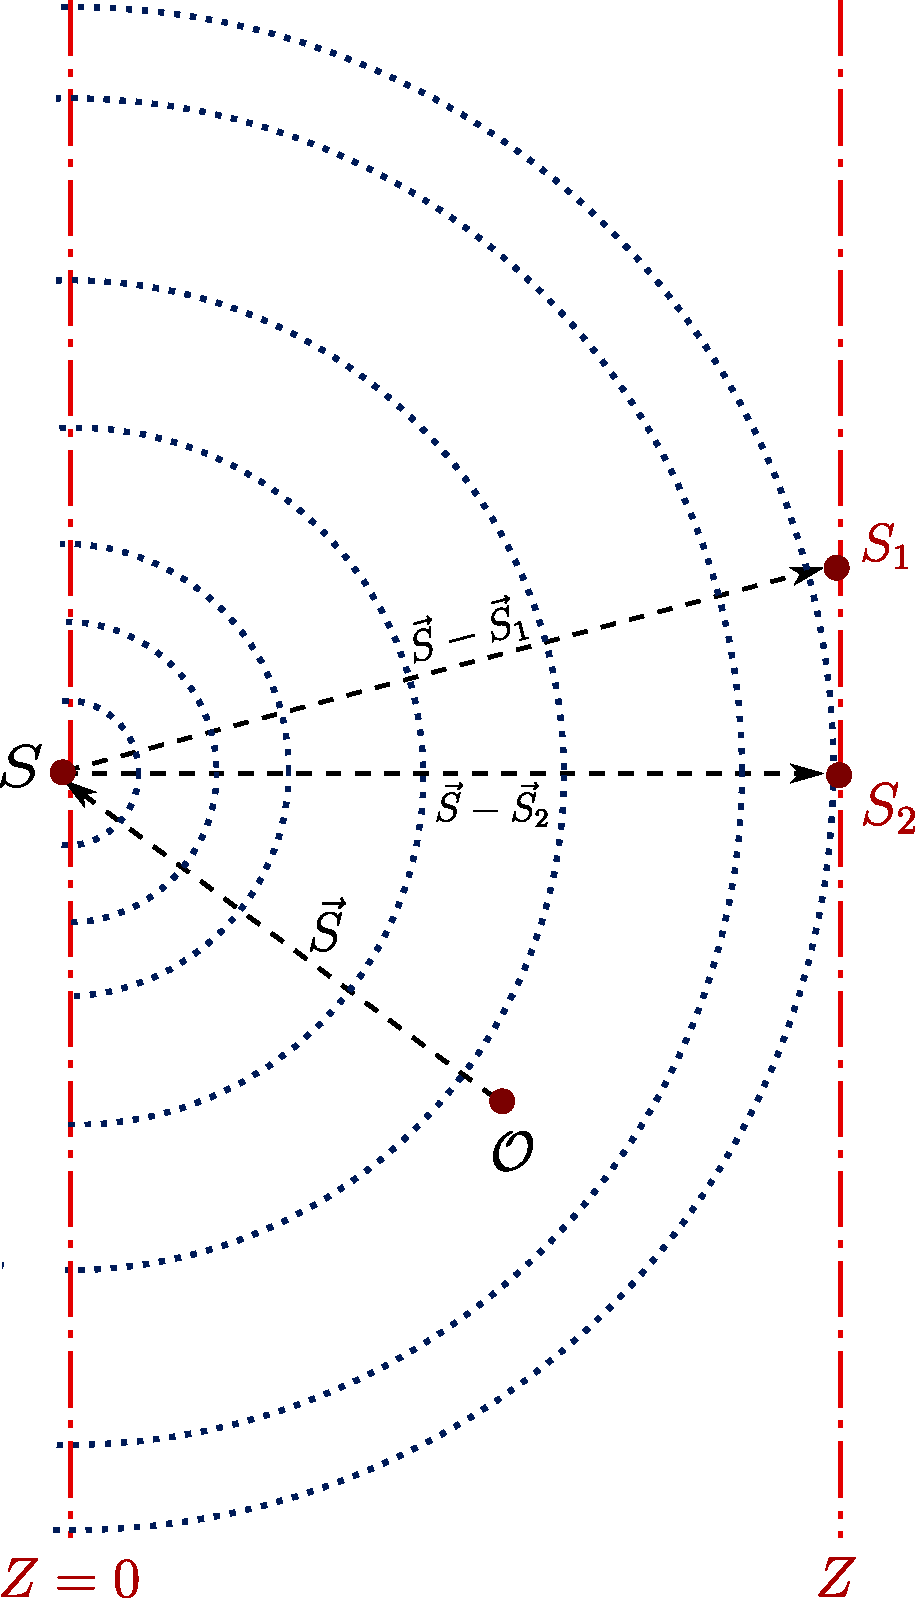
\includegraphics[width=0.65\linewidth]{Capitulo 2/Figuras/FourierGamma}
			\caption{La coherencia mutua propagada al campo lejano es la transformada de Fourier de la distribución de intensidad $\Gamma_0(\vec{S})$ de la fuente.}
			\label{fig:fouriergamma}
		\end{figure}

		¿Cómo podemos saber en qué dirección fluye el tiempo? Esto puede sonar como una pregunta bastante fuera de contexto para estos apuntes, pero si pudiéramos viajar a la época dorada de Boltzmann, encontraríamos un acalorado debate de la época sobre cómo la física estadística le da una dirección al tiempo, una \textit{flecha}. Parafraseando a Boltzmann, se dice que \textit{el tiempo avanza en la dirección en que las correlaciones aumentan}. Si observamos el teorema de van Cittert-Zernike, podemos partir de dos fuentes completamente no correlacionadas que, sin embargo, a medida que se propagan, van correlacionándose gradualmente; el tiempo crece y con él la coherencia, hasta llegar a un punto en el que la radiación de esas fuentes es coherente. Este es, sin duda, uno de los resultados más fuertes y hermosos que podemos encontrar en la física estadística.


	\chapter{Mecánica analítica y el principio de acción}\label{chap:MecanicaAnalitica}
	\thispagestyle{empty}
	\vspace*{2cm}
	\begin{center}
		{\itshape\Huge De todos los caminos que la naturaleza podría seguir, escoge aquel sobre el cual la acción no cambia. \par}
		\vspace{1cm}
		\epigraph{``La naturaleza es siempre ahorrativa en la acción''}{-- Pierre Louis Moreau de Maupertuis}
	\end{center}
	\clearpage

	\section{Breve historia del principio de acción: de Fermat a Feynman}

    Existe en la física una idea que reaparece, con ropajes distintos, en casi todos los niveles de descripción de la naturaleza: la idea de que el comportamiento efectivo de un sistema puede obtenerse exigiendo que cierta cantidad global, acumulada a lo largo de toda su historia, sea estacionaria. No se trata de una ley de fuerzas ni de una prescripción local sobre lo que ocurre en un instante, sino de una condición sobre la trayectoria completa, y esa diferencia de perspectiva, aparentemente solo estética, resultó ser el hilo conductor que llevó de la mecánica de Newton a la mecánica cuántica y de allí a la integral de camino que usaremos más adelante para describir la propagación de los fotones.

    El primer eco de esta idea es anterior en muchos siglos a la mecánica. Herón de Alejandría, en el siglo I de nuestra era, observó que un rayo de luz reflejado en un espejo plano recorre, entre dos puntos dados, el camino más corto de todos los que tocan la superficie, y esa observación permaneció como una curiosidad geométrica hasta que Pierre de Fermat, hacia 1662, la generalizó a la refracción sustituyendo la longitud geométrica por el tiempo de recorrido. La ley de Snell, que hasta entonces era un hecho experimental sin explicación, quedaba así deducida de un principio de economía: la luz escoge, entre todos los caminos concebibles, aquel para el cual el tiempo es estacionario. El resultado incomodó profundamente a sus contemporáneos, y la objeción que se le hizo es la misma que se repetirá en cada nueva encarnación del principio, a saber, que un criterio de este tipo parece atribuir a la luz el conocimiento anticipado de su destino, pues para escoger el camino óptimo habría que comparar todos los caminos posibles antes de recorrer ninguno.

    La traducción de esta idea al lenguaje de la mecánica fue obra de Pierre Louis Moreau de Maupertuis, quien en 1744 propuso su \textit{principio de mínima acción} definiendo la acción como la integral del producto de la masa por la velocidad y por el elemento de camino \citep{maupertuis1744accord}. La motivación de Maupertuis era en buena medida teológica, pues veía en la economía de la naturaleza una prueba de la sabiduría de su creador, y su formulación era tan vaga que resultaba difícil de aplicar a cualquier problema concreto; pero la intuición era correcta. Ese mismo año, y con una claridad matemática que Maupertuis nunca alcanzó, Leonhard Euler publicó el tratado en el que establece las condiciones que debe cumplir una curva para hacer estacionaria una integral \citep{euler1744methodus}, fundando de paso el cálculo de variaciones como disciplina. Euler demostró para el caso de una partícula sometida a fuerzas centrales que la trayectoria newtoniana es exactamente la que hace estacionaria la acción de Maupertuis, con lo cual el principio dejaba de ser una conjetura metafísica y pasaba a ser un teorema.

    El paso decisivo lo dio Joseph Louis Lagrange con la publicación de la \textit{Méchanique Analitique} en 1788 \citep{lagrange1788mecanique}, un libro del que su autor se enorgullecía de que no contuviera una sola figura. Lagrange comprendió que la verdadera ventaja del método variacional no reside en la economía de la naturaleza sino en la libertad de coordenadas: si las ecuaciones de movimiento se obtienen exigiendo que una integral escalar sea estacionaria, entonces tendrán la misma forma en cualquier sistema de coordenadas que se escoja, porque un escalar no sabe en qué coordenadas se le está evaluando. Las ligaduras, que en el lenguaje newtoniano obligan a introducir fuerzas de reacción desconocidas, desaparecen del problema sin más que escoger coordenadas adaptadas a ellas. Esa es la razón por la cual la mecánica lagrangiana se impuso, y no ninguna consideración sobre la economía del universo.

    Medio siglo más tarde William Rowan Hamilton, que había llegado a la mecánica desde la óptica, dio a la teoría su forma definitiva en dos memorias publicadas en 1834 y 1835 \citep{hamilton1834general, hamilton1835second}. Hamilton había demostrado en 1828 que todo sistema óptico puede describirse mediante una única función, la \textit{función característica}, cuyas derivadas parciales dan las direcciones de los rayos \citep{hamilton1828theory}, y al trasladar esa construcción a la mecánica descubrió que la misma estructura gobierna el movimiento de las partículas: existe una función de las coordenadas y del tiempo cuyas derivadas parciales son los momentos. La analogía es tan precisa que Hamilton la formuló explícitamente como un diccionario entre la óptica geométrica y la mecánica de partículas, con los frentes de onda correspondiendo a superficies de acción constante y los rayos a trayectorias. \textbf{Aquella analogía, que durante casi un siglo pareció una curiosidad formal sin contenido físico, resultó ser la pista que Schrödinger siguió en 1926 para construir la mecánica ondulatoria.} Carl Gustav Jacob Jacobi completó el programa poco después, mostrando que la función de Hamilton satisface una ecuación diferencial en derivadas parciales cuya solución completa resuelve por completo el problema mecánico \citep{jacobi1866vorlesungen}.

    El andamiaje algebraico que sostiene todo esto se había construido en paralelo. Siméon Denis Poisson había introducido en 1809 los corchetes que llevan su nombre al estudiar cómo varían las constantes de integración de un problema perturbado \citep{poisson1809memoire}, sin sospechar que estaba escribiendo la estructura algebraica que un siglo después Dirac reconocería como el límite clásico del conmutador cuántico. Joseph Liouville demostró en 1838 que el flujo generado por las ecuaciones de Hamilton conserva el volumen en el espacio de fase \citep{liouville1838note}, resultado que es el fundamento de la mecánica estadística. Y en 1918 Emmy Noether cerró el círculo conceptual al demostrar que toda simetría continua de la acción lleva asociada una cantidad conservada \citep{noether1918invariante}, convirtiendo las leyes de conservación, que hasta entonces eran hechos empíricos independientes, en consecuencias necesarias de la estructura del lagrangiano.

    La historia que nos interesa aquí, sin embargo, no termina en la mecánica clásica. En 1924 Louis de Broglie propuso que a toda partícula de momento $p$ le corresponde una longitud de onda $\lambda = h/p$ \citep{debroglie1924recherches}, y al hacerlo convirtió la analogía de Hamilton en una afirmación física: si la mecánica clásica es a la mecánica verdadera lo que la óptica geométrica es a la óptica ondulatoria, entonces debe existir una ecuación de ondas cuyo límite de longitud de onda corta reproduzca la ecuación de Hamilton-Jacobi. Erwin Schrödinger buscó esa ecuación durante el invierno de 1925 y la encontró en enero de 1926 \citep{schrodinger1926quantisierung}, y el camino que siguió, que reconstruiremos paso a paso en este capítulo, parte precisamente de la ecuación de Hamilton-Jacobi y de una sustitución exponencial. Siete años más tarde Paul Dirac observó que la amplitud de transición de la mecánica cuántica \textit{corresponde} a la exponencial de la acción clásica dividida por $\hbar$ \citep{dirac1933lagrangian}, y en 1948 Richard Feynman convirtió ese \textit{corresponde} en una igualdad, mostrando que la amplitud entre dos puntos es la suma de $e^{iS/\hbar}$ sobre todos los caminos que los unen \citep{feynman1948space}. Con ello la objeción que se le había hecho a Fermat tres siglos antes quedaba finalmente respondida: la luz no escoge un camino, los recorre todos, y el camino clásico es simplemente aquel en cuya vecindad las fases no se cancelan.

    Este capítulo recorre esa cadena en orden. Construiremos las ecuaciones de Lagrange desde la mecánica newtoniana, las obtendremos de nuevo a partir del principio de Hamilton, pasaremos al formalismo hamiltoniano mediante la transformada de Legendre, deduciremos la ecuación de Hamilton-Jacobi, la usaremos para llegar a la ecuación de Schrödinger siguiendo el razonamiento original, extenderemos el formalismo a sistemas continuos, que es lo que exige la cuantización del campo electromagnético del capítulo siguiente, y terminaremos con la integral de camino y con el propagador del oscilador armónico, que es la expresión de la que parte el capítulo dedicado a la propagación de los fotones.

\section{De Newton a Lagrange}

        La mecánica newtoniana describe un sistema de $N$ partículas mediante $N$ ecuaciones vectoriales
        \begin{equation}\label{eq:Newton}
            \dot{\mathbf{p}}_{i} = \mathbf{F}_{i}, \qquad \mathbf{p}_{i} = m_{i}\dot{\mathbf{r}}_{i}, \qquad i = 1,\ldots,N,
        \end{equation}
        lo que en coordenadas cartesianas equivale a $3N$ ecuaciones diferenciales de segundo orden. Si las fuerzas fuesen todas conocidas de antemano el problema estaría cerrado, pero en la práctica casi nunca lo están, porque los sistemas reales están sometidos a \textit{ligaduras}: la cuenta de un ábaco está obligada a permanecer sobre el alambre, las partículas de un sólido rígido mantienen fijas sus distancias mutuas, y la masa de un péndulo no puede alejarse del punto de suspensión más allá de la longitud del hilo. Las fuerzas que imponen estas condiciones, la reacción del alambre, las fuerzas internas del sólido, la tensión del hilo, no están dadas por ninguna ley constitutiva: son precisamente las que hacen falta, instante a instante, para que la condición se cumpla, de modo que son incógnitas del problema y no datos.

        Diremos que una ligadura es \textit{holónoma} cuando puede expresarse como una relación funcional entre las coordenadas y el tiempo,
        \begin{equation}\label{eq:Holonoma}
            f_{\alpha}(\mathbf{r}_{1},\mathbf{r}_{2},\ldots,\mathbf{r}_{N},t) = 0, \qquad \alpha = 1,\ldots,k,
        \end{equation}
        y \textit{no holónoma} en caso contrario, como ocurre con la condición de rodadura sin deslizamiento de una esfera sobre un plano, que involucra velocidades y no es integrable. Restringiremos en adelante el tratamiento al caso holónomo, que es el único que necesitaremos.

        La utilidad de \eqref{eq:Holonoma} es doble. Por una parte, cada una de las $k$ ligaduras elimina una coordenada independiente, de manera que el número de \textit{grados de libertad} del sistema pasa a ser
        \begin{equation}\label{eq:GradosLibertad}
            n = 3N - k .
        \end{equation}
        Por otra parte, y esto es lo esencial, las $k$ relaciones permiten introducir $n$ cantidades independientes $q_{1},\ldots,q_{n}$, las \textit{coordenadas generalizadas}, en términos de las cuales las posiciones quedan determinadas,
        \begin{equation}\label{eq:CoordGen}
            \mathbf{r}_{i} = \mathbf{r}_{i}(q_{1},q_{2},\ldots,q_{n},t), \qquad i = 1,\ldots,N .
        \end{equation}
        Las coordenadas generalizadas no tienen por qué ser longitudes: pueden ser ángulos, áreas, amplitudes de un modo normal o cualquier otro parámetro conveniente, y de hecho la libertad de escogerlas a conveniencia es lo que hace poderoso a todo el formalismo. En el capítulo siguiente veremos que las coordenadas generalizadas naturales del campo electromagnético en una cavidad son las amplitudes $q_{\mathbf{k},\lambda}(t)$ de sus modos normales, que no son posiciones de ninguna partícula.

        Nótese desde ahora que \eqref{eq:CoordGen} incorpora la ligadura de manera automática. Cualquier movimiento descrito por funciones $q_{j}(t)$ arbitrarias satisface \eqref{eq:Holonoma} idénticamente, porque las ligaduras ya fueron usadas al construir la parametrización. Las fuerzas de ligadura, que en el lenguaje newtoniano eran incógnitas adicionales, desaparecen del problema no porque se las haya calculado sino porque se ha escogido un lenguaje en el que no pueden ser nombradas.

        Para explotar esa idea necesitamos una noción de desplazamiento que respete las ligaduras. Llamaremos \textit{desplazamiento virtual} $\delta\mathbf{r}_{i}$ a un cambio infinitesimal de la configuración del sistema, compatible con las ligaduras, realizado a tiempo congelado. El adjetivo virtual indica que no se trata de un desplazamiento efectivamente recorrido durante la evolución, sino de una comparación imaginaria entre configuraciones simultáneas, y la congelación del tiempo es esencial: el desplazamiento real $d\mathbf{r}_{i}$ incluye el término $(\partial\mathbf{r}_{i}/\partial t)\,dt$ que proviene del movimiento de las propias ligaduras, mientras que el virtual no,
        \begin{equation}\label{eq:DespVirtual}
            \delta\mathbf{r}_{i} = \sum_{j=1}^{n}\frac{\partial\mathbf{r}_{i}}{\partial q_{j}}\,\delta q_{j},
            \qquad\text{frente a}\qquad
            d\mathbf{r}_{i} = \sum_{j=1}^{n}\frac{\partial\mathbf{r}_{i}}{\partial q_{j}}\,dq_{j} + \frac{\partial\mathbf{r}_{i}}{\partial t}\,dt .
        \end{equation}

        La hipótesis física que permite eliminar las fuerzas de ligadura es la siguiente, y hay que enunciarla con precisión porque todo lo demás descansa sobre ella.

        \begin{Assumption}\label{sup:TrabajoVirtual}
            El trabajo total realizado por las fuerzas de ligadura sobre cualquier desplazamiento virtual del sistema es nulo.
        \end{Assumption}

        El supuesto se cumple en todos los casos de interés práctico y su contenido geométrico es transparente: una fuerza de ligadura es perpendicular a la superficie sobre la cual obliga a moverse al sistema, y un desplazamiento virtual es tangente a esa superficie, de modo que su producto escalar se anula. La reacción normal de una mesa no realiza trabajo sobre un cuerpo que se desliza horizontalmente, la tensión de un hilo inextensible no realiza trabajo sobre la masa del péndulo porque es perpendicular al arco, y las fuerzas internas de un sólido rígido no realizan trabajo neto porque las distancias mutuas no cambian. El caso que queda excluido es el de la fricción de deslizamiento, que es antiparalela al desplazamiento y por tanto realiza trabajo negativo; los sistemas disipativos requieren un tratamiento aparte y no los consideraremos.

        Separamos entonces la fuerza sobre cada partícula en su parte aplicada y su parte de ligadura,
        \begin{equation}\label{eq:FuerzaSeparada}
            \mathbf{F}_{i} = \mathbf{F}_{i}^{(a)} + \mathbf{f}_{i},
        \end{equation}
        y escribamos la segunda ley \eqref{eq:Newton} en la forma en que d'Alembert la dispuso, pasando todo a un miembro,
        \begin{equation}\label{eq:dAlembertPartida}
            \mathbf{F}_{i}^{(a)} + \mathbf{f}_{i} - \dot{\mathbf{p}}_{i} = 0 .
        \end{equation}
        Multiplicando escalarmente por el desplazamiento virtual de la partícula $i$ y sumando sobre todas las partículas,
        \begin{equation}\label{eq:SumaVirtual}
            \sum_{i=1}^{N}\left(\mathbf{F}_{i}^{(a)} - \dot{\mathbf{p}}_{i}\right)\cdot\delta\mathbf{r}_{i}
            + \textcolor{red}{\sum_{i=1}^{N}\mathbf{f}_{i}\cdot\delta\mathbf{r}_{i}} = 0,
        \end{equation}
        donde el término marcado en rojo se anula en virtud del supuesto \ref{sup:TrabajoVirtual}. Queda así el \textit{principio de d'Alembert},
        \begin{equation}\label{eq:dAlembert}
            \sum_{i=1}^{N}\left(\mathbf{F}_{i}^{(a)} - \dot{\mathbf{p}}_{i}\right)\cdot\delta\mathbf{r}_{i} = 0,
        \end{equation}
        en el cual ya no aparece ninguna fuerza desconocida. El precio pagado es que \eqref{eq:dAlembert} no puede leerse componente a componente, porque los $\delta\mathbf{r}_{i}$ no son independientes entre sí: están ligados por \eqref{eq:Holonoma}. Ese es exactamente el problema que resuelven las coordenadas generalizadas, cuyas variaciones $\delta q_{j}$ sí son independientes por construcción.

        Vamos a traducir \eqref{eq:dAlembert} al lenguaje de las $q_{j}$. El primer término define las \textit{fuerzas generalizadas}: sustituyendo el desplazamiento virtual \eqref{eq:DespVirtual} e intercambiando el orden de las sumas,
        \begin{equation}\label{eq:FuerzaGen}
            \sum_{i=1}^{N}\mathbf{F}_{i}^{(a)}\cdot\delta\mathbf{r}_{i}
            = \sum_{i=1}^{N}\sum_{j=1}^{n}\mathbf{F}_{i}^{(a)}\cdot\frac{\partial\mathbf{r}_{i}}{\partial q_{j}}\,\delta q_{j}
            \equiv \sum_{j=1}^{n} Q_{j}\,\delta q_{j},
            \qquad
            Q_{j} \equiv \sum_{i=1}^{N}\mathbf{F}_{i}^{(a)}\cdot\frac{\partial\mathbf{r}_{i}}{\partial q_{j}} .
        \end{equation}
        Adviértase que $Q_{j}$ no tiene por qué tener dimensiones de fuerza; si $q_{j}$ es un ángulo, entonces $Q_{j}$ es un torque. Lo único que la definición garantiza es que el producto $Q_{j}\delta q_{j}$ tenga dimensiones de trabajo, que es lo que exige la consistencia de \eqref{eq:FuerzaGen}.

        El segundo término requiere más cuidado, y lo trabajaremos en detalle porque de él sale toda la estructura. Partimos de
        \begin{equation}\label{eq:TerminoInercial}
            \sum_{i=1}^{N}\dot{\mathbf{p}}_{i}\cdot\delta\mathbf{r}_{i}
            = \sum_{i=1}^{N}\sum_{j=1}^{n} m_{i}\ddot{\mathbf{r}}_{i}\cdot\frac{\partial\mathbf{r}_{i}}{\partial q_{j}}\,\delta q_{j},
        \end{equation}
        y observamos que el sumando admite reescribirse como la derivada temporal de un producto menos el término que sobra, que es la regla del producto leída al revés,
        \begin{equation}\label{eq:ReglaProductoInversa}
            m_{i}\ddot{\mathbf{r}}_{i}\cdot\frac{\partial\mathbf{r}_{i}}{\partial q_{j}}
            = \frac{d}{dt}\left(m_{i}\dot{\mathbf{r}}_{i}\cdot\frac{\partial\mathbf{r}_{i}}{\partial q_{j}}\right)
            - m_{i}\dot{\mathbf{r}}_{i}\cdot\frac{d}{dt}\left(\frac{\partial\mathbf{r}_{i}}{\partial q_{j}}\right).
        \end{equation}
        El paso se justifica porque el primer término de la derecha, al derivarse, produce el término de la izquierda más el segundo término de la derecha con signo contrario, de modo que la identidad es exacta y no una aproximación.

        Necesitamos ahora dos identidades auxiliares, y las demostramos por separado porque son el verdadero contenido técnico de la deducción. La primera relaciona la derivada de la posición respecto de una coordenada generalizada con la derivada de la velocidad respecto de la velocidad generalizada. Derivando \eqref{eq:CoordGen} respecto del tiempo mediante la regla de la cadena,
        \begin{equation}\label{eq:VelocidadCadena}
            \mathbf{v}_{i} \equiv \dot{\mathbf{r}}_{i} = \sum_{l=1}^{n}\frac{\partial\mathbf{r}_{i}}{\partial q_{l}}\dot{q}_{l} + \frac{\partial\mathbf{r}_{i}}{\partial t},
        \end{equation}
        y derivando esta expresión respecto de $\dot{q}_{j}$ notamos que las funciones $\partial\mathbf{r}_{i}/\partial q_{l}$ y $\partial\mathbf{r}_{i}/\partial t$ dependen solamente de las coordenadas y del tiempo, nunca de las velocidades, de manera que se comportan como constantes en esa derivación y solo sobrevive el término $l = j$,
        \begin{equation}\label{eq:CancelacionPuntos}
            \frac{\partial\mathbf{v}_{i}}{\partial\dot{q}_{j}}
            = \sum_{l=1}^{n}\frac{\partial\mathbf{r}_{i}}{\partial q_{l}}\,\frac{\partial\dot{q}_{l}}{\partial\dot{q}_{j}}
            + \textcolor{red}{\frac{\partial}{\partial\dot{q}_{j}}\frac{\partial\mathbf{r}_{i}}{\partial t}}
            = \sum_{l=1}^{n}\frac{\partial\mathbf{r}_{i}}{\partial q_{l}}\,\delta_{lj}
            = \frac{\partial\mathbf{r}_{i}}{\partial q_{j}} .
        \end{equation}
        Esta identidad, conocida como \textit{cancelación de los puntos}, dice que en lo que respecta a la derivación las velocidades generalizadas entran linealmente en las velocidades cartesianas con coeficientes que son exactamente los vectores tangentes a la superficie de configuración.

        La segunda identidad afirma que la derivada temporal total y la derivada parcial respecto de $q_{j}$ conmutan cuando actúan sobre la posición. Calculando explícitamente el miembro izquierdo mediante la regla de la cadena,
        \begin{equation}\label{eq:ConmutanDerivadas}
            \frac{d}{dt}\left(\frac{\partial\mathbf{r}_{i}}{\partial q_{j}}\right)
            = \sum_{l=1}^{n}\frac{\partial^{2}\mathbf{r}_{i}}{\partial q_{l}\partial q_{j}}\dot{q}_{l}
            + \frac{\partial^{2}\mathbf{r}_{i}}{\partial t\,\partial q_{j}}
            = \frac{\partial}{\partial q_{j}}\left(\sum_{l=1}^{n}\frac{\partial\mathbf{r}_{i}}{\partial q_{l}}\dot{q}_{l} + \frac{\partial\mathbf{r}_{i}}{\partial t}\right)
            = \frac{\partial\mathbf{v}_{i}}{\partial q_{j}},
        \end{equation}
        donde hemos usado la igualdad de las derivadas parciales cruzadas, válida porque las funciones $\mathbf{r}_{i}$ son de clase $C^{2}$, y el hecho de que $\dot{q}_{l}$ no depende de $q_{j}$, lo que permite introducir la derivada parcial dentro de la suma.

        Sustituyendo \eqref{eq:CancelacionPuntos} y \eqref{eq:ConmutanDerivadas} en \eqref{eq:ReglaProductoInversa} obtenemos
        \begin{equation}\label{eq:TerminoInercial2}
            m_{i}\ddot{\mathbf{r}}_{i}\cdot\frac{\partial\mathbf{r}_{i}}{\partial q_{j}}
            = \frac{d}{dt}\left(m_{i}\mathbf{v}_{i}\cdot\frac{\partial\mathbf{v}_{i}}{\partial\dot{q}_{j}}\right)
            - m_{i}\mathbf{v}_{i}\cdot\frac{\partial\mathbf{v}_{i}}{\partial q_{j}},
        \end{equation}
        y ambos términos son ahora derivadas de una misma cantidad escalar. En efecto, usando que
        \begin{equation}\label{eq:DerivadaCuadrado}
            \frac{\partial}{\partial\dot{q}_{j}}\left(\frac{1}{2}m_{i}v_{i}^{2}\right) = m_{i}\mathbf{v}_{i}\cdot\frac{\partial\mathbf{v}_{i}}{\partial\dot{q}_{j}},
            \qquad
            \frac{\partial}{\partial q_{j}}\left(\frac{1}{2}m_{i}v_{i}^{2}\right) = m_{i}\mathbf{v}_{i}\cdot\frac{\partial\mathbf{v}_{i}}{\partial q_{j}},
        \end{equation}
        y sumando sobre todas las partículas, aparece la energía cinética total
        \begin{equation}\label{eq:EnergiaCinetica}
            T = \sum_{i=1}^{N}\frac{1}{2}m_{i}v_{i}^{2},
        \end{equation}
        de modo que \eqref{eq:TerminoInercial} se convierte en
        \begin{equation}\label{eq:TerminoInercial3}
            \sum_{i=1}^{N}\dot{\mathbf{p}}_{i}\cdot\delta\mathbf{r}_{i}
            = \sum_{j=1}^{n}\left[\frac{d}{dt}\left(\frac{\partial T}{\partial\dot{q}_{j}}\right) - \frac{\partial T}{\partial q_{j}}\right]\delta q_{j} .
        \end{equation}

        Llevando \eqref{eq:FuerzaGen} y \eqref{eq:TerminoInercial3} al principio de d'Alembert \eqref{eq:dAlembert} resulta
        \begin{equation}\label{eq:dAlembertGen}
            \sum_{j=1}^{n}\left[\frac{d}{dt}\left(\frac{\partial T}{\partial\dot{q}_{j}}\right) - \frac{\partial T}{\partial q_{j}} - Q_{j}\right]\delta q_{j} = 0 .
        \end{equation}
        Aquí sí podemos leer la ecuación componente a componente, y esta es la ganancia de todo el rodeo: como las coordenadas generalizadas son independientes, las variaciones $\delta q_{j}$ pueden escogerse arbitrariamente y una a una, de manera que escogiendo $\delta q_{1}\neq 0$ con todas las demás nulas se concluye que el corchete correspondiente a $j=1$ se anula, y repitiendo el argumento para cada índice,
        \begin{equation}\label{eq:LagrangeT}
            \frac{d}{dt}\left(\frac{\partial T}{\partial\dot{q}_{j}}\right) - \frac{\partial T}{\partial q_{j}} = Q_{j}, \qquad j = 1,\ldots,n .
        \end{equation}

        Falta un último paso para llegar a la forma canónica. Supongamos que las fuerzas aplicadas derivan de un potencial escalar $V(\mathbf{r}_{1},\ldots,\mathbf{r}_{N},t)$, es decir $\mathbf{F}_{i}^{(a)} = -\nabla_{i}V$. Entonces, por la definición \eqref{eq:FuerzaGen} y la regla de la cadena,
        \begin{equation}\label{eq:FuerzaGenPotencial}
            Q_{j} = -\sum_{i=1}^{N}\nabla_{i}V\cdot\frac{\partial\mathbf{r}_{i}}{\partial q_{j}} = -\frac{\partial V}{\partial q_{j}},
        \end{equation}
        y sustituyendo en \eqref{eq:LagrangeT} y agrupando todo en un miembro,
        \begin{equation}\label{eq:LagrangePaso}
            \frac{d}{dt}\left(\frac{\partial T}{\partial\dot{q}_{j}}\right) - \frac{\partial (T-V)}{\partial q_{j}} = 0 .
        \end{equation}
        Como el potencial no depende de las velocidades, se cumple $\partial V/\partial\dot{q}_{j} = 0$ y por tanto podemos sumar ese cero dentro de la derivada temporal sin alterar nada,
        \begin{equation}\label{eq:SumaCero}
            \frac{\partial T}{\partial\dot{q}_{j}} = \frac{\partial T}{\partial\dot{q}_{j}} - \textcolor{blue}{\frac{\partial V}{\partial\dot{q}_{j}}} = \frac{\partial(T-V)}{\partial\dot{q}_{j}},
        \end{equation}
        donde el término en azul se ha introducido deliberadamente porque vale cero. Definiendo la \textit{función lagrangiana}
        \begin{equation}\label{eq:Lagrangiano}
            L(q,\dot{q},t) \equiv T - V,
        \end{equation}
        las dos derivadas quedan referidas a un mismo objeto y obtenemos las \textit{ecuaciones de Lagrange}
        \begin{equation}\label{eq:EulerLagrange}
            \boxed{\;\frac{d}{dt}\left(\frac{\partial L}{\partial\dot{q}_{j}}\right) - \frac{\partial L}{\partial q_{j}} = 0, \qquad j = 1,\ldots,n .\;}
        \end{equation}

        Lo que se ha conseguido es mucho más de lo que sugiere el aspecto inocente de \eqref{eq:EulerLagrange}. Hemos pasado de $3N$ ecuaciones vectoriales acopladas, con $k$ fuerzas de ligadura desconocidas, a $n = 3N-k$ ecuaciones escalares sin incógnitas espurias, y toda la dinámica del sistema está codificada en una única función escalar $L$. La diferencia $T-V$ no tiene, hay que decirlo, ninguna interpretación física directa: no es una energía que se conserve ni una cantidad que se mida en el laboratorio, y el intento de dotarla de significado intuitivo ha producido más confusión que claridad. Su importancia es estructural y no sustancial: es la función cuya estacionariedad reproduce las ecuaciones de movimiento, y eso basta. La justificación profunda de por qué debe ser precisamente $T-V$ y no otra combinación la daremos en la sección siguiente, donde las mismas ecuaciones surgirán de un principio variacional que no presupone las leyes de Newton.

\section{El principio de Hamilton y el cálculo de variaciones}

        La deducción anterior partió de las leyes de Newton y llegó a las ecuaciones de Lagrange. Vamos a invertir ahora el orden lógico, postulando un principio integral del que las ecuaciones de movimiento se deduzcan, porque esa formulación es la que se generaliza sin cambios a los campos, a la relatividad y a la teoría cuántica, mientras que la segunda ley de Newton no lo hace.

        Consideremos un sistema de $n$ grados de libertad y fijemos dos configuraciones, la inicial $q(t_{1}) = q^{(1)}$ y la final $q(t_{2}) = q^{(2)}$. Llamaremos \textit{camino} a cualquier función $q(t)$ suficientemente suave que una ambas configuraciones en el intervalo dado, sin exigirle que satisfaga las ecuaciones de movimiento; la inmensa mayoría de los caminos así definidos son físicamente imposibles, y eso es intencional.

        \begin{myDef}\label{def:Accion}
            Se llama \textit{acción} del sistema al funcional que a cada camino $q(t)$ le asigna el número real
            \begin{equation}\label{eq:Accion}
                S[q] = \int_{t_{1}}^{t_{2}} L\left(q(t),\dot{q}(t),t\right)\,dt .
            \end{equation}
        \end{myDef}

        La acción no es una función de un número sino de una función entera, razón por la cual se la llama funcional y se escribe con corchetes. Sus dimensiones son las de energía por tiempo, que son también las de momento por longitud y las de momento angular; que $\hbar$ tenga precisamente esas dimensiones no es una coincidencia sino la primera señal de que la acción es la cantidad que mide, en unidades cuánticas, cuán clásico es un sistema.

        El principio que sustituye a las leyes de Newton es el siguiente.

        \begin{Assumption}[Principio de Hamilton]\label{sup:Hamilton}
            El movimiento efectivo del sistema entre dos configuraciones fijas es aquel para el cual la acción \eqref{eq:Accion} es estacionaria frente a variaciones infinitesimales del camino que dejan fijos los extremos.
        \end{Assumption}

        Hay que insistir en la palabra estacionaria y no mínima, pese a que el principio se llame tradicionalmente de mínima acción. Para tiempos suficientemente cortos el camino clásico efectivamente minimiza la acción, pero para tiempos largos puede tratarse de un punto silla, y el ejemplo estándar es el del oscilador armónico más allá de medio período. Lo que la física exige es que la primera variación se anule, no que el valor sea el menor posible.

        Para dar contenido operativo al supuesto \ref{sup:Hamilton} hay que definir qué significa variar un camino. Introducimos, como en la figura \ref{fig:VariacionCamino}, una familia uniparamétrica de caminos
        \begin{equation}\label{eq:FamiliaCaminos}
            q_{j}(t,\varepsilon) = q_{j}(t,0) + \varepsilon\,\eta_{j}(t),
        \end{equation}
        donde $q_{j}(t,0)$ es el camino sobre el cual queremos evaluar la estacionariedad, $\varepsilon$ es un parámetro real infinitesimal y las funciones $\eta_{j}(t)$ son arbitrarias salvo por dos condiciones: deben ser derivables y deben anularse en los extremos,
        \begin{equation}\label{eq:ExtremosFijos}
            \eta_{j}(t_{1}) = \eta_{j}(t_{2}) = 0, \qquad j = 1,\ldots,n,
        \end{equation}
        que es la traducción matemática de que todos los caminos de la familia parten de la misma configuración inicial y llegan a la misma configuración final. Derivando \eqref{eq:FamiliaCaminos} respecto del tiempo, la variación de la velocidad resulta ser la derivada de la variación,
        \begin{equation}\label{eq:VariacionVelocidad}
            \dot{q}_{j}(t,\varepsilon) = \dot{q}_{j}(t,0) + \varepsilon\,\dot{\eta}_{j}(t),
            \qquad\text{es decir}\qquad
            \delta\dot{q}_{j} = \frac{d}{dt}\,\delta q_{j},
        \end{equation}
        propiedad que usaremos de inmediato y que es cierta porque la variación se toma a tiempo fijo mientras que la derivada se toma a $\varepsilon$ fijo, de modo que ambas operaciones conmutan.

        Sobre esta familia la acción se convierte en una función ordinaria del parámetro,
        \begin{equation}\label{eq:AccionEpsilon}
            S(\varepsilon) = \int_{t_{1}}^{t_{2}} L\left(q(t,\varepsilon),\dot{q}(t,\varepsilon),t\right)dt,
        \end{equation}
        y la condición de estacionariedad se reduce a la condición de que la derivada ordinaria de $S(\varepsilon)$ se anule en $\varepsilon = 0$ para toda elección de las funciones $\eta_{j}$. Definimos por ello la \textit{primera variación} de la acción como
        \begin{equation}\label{eq:PrimeraVariacion}
            \delta S \equiv \left.\frac{dS}{d\varepsilon}\right|_{\varepsilon=0}\varepsilon .
        \end{equation}

        \begin{figure}[htbp]
            \centering
            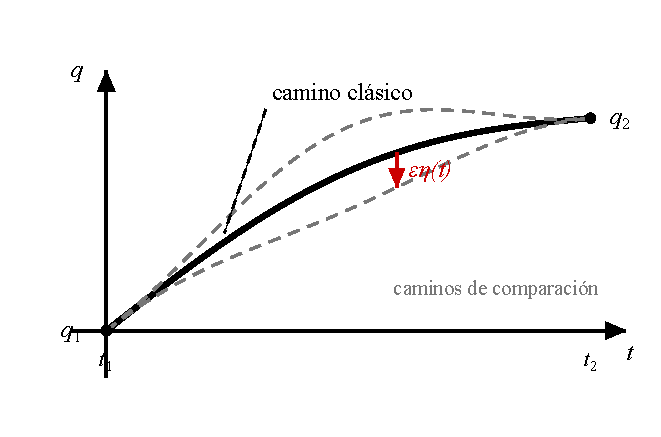
\includegraphics[width=0.62\linewidth]{Capitulo 3/Figuras/VariacionCamino.pdf}
            \caption{El camino efectivo y los caminos de comparación que se usan para variarlo. Todos parten de la misma configuración inicial y llegan a la misma final, de modo que la desviación $\varepsilon\eta(t)$ se anula en los dos extremos.}
            \label{fig:VariacionCamino}
        \end{figure}

        Podemos calcular esa derivada explícitamente. Derivando bajo el signo integral, lo que es lícito porque el integrando es continuo junto con su derivada respecto de $\varepsilon$ en un intervalo compacto, y aplicando la regla de la cadena,
        \begin{equation}\label{eq:DerivadaAccion}
            \frac{dS}{d\varepsilon} = \int_{t_{1}}^{t_{2}}\sum_{j=1}^{n}\left[\frac{\partial L}{\partial q_{j}}\frac{\partial q_{j}}{\partial\varepsilon} + \frac{\partial L}{\partial\dot{q}_{j}}\frac{\partial\dot{q}_{j}}{\partial\varepsilon}\right]dt
            = \int_{t_{1}}^{t_{2}}\sum_{j=1}^{n}\left[\frac{\partial L}{\partial q_{j}}\eta_{j} + \frac{\partial L}{\partial\dot{q}_{j}}\dot{\eta}_{j}\right]dt,
        \end{equation}
        donde el término $\partial L/\partial t$ no aparece porque el tiempo no depende de $\varepsilon$.

        El obstáculo es que en \eqref{eq:DerivadaAccion} figuran tanto $\eta_{j}$ como $\dot{\eta}_{j}$, y mientras eso sea así no podremos concluir nada sobre el corchete, porque una función y su derivada no son independientes. El recurso es integrar por partes el segundo término para transferir la derivada de $\eta_{j}$ hacia el otro factor. Escribiendo la regla del producto al revés,
        \begin{equation}\label{eq:ParaPartes}
            \frac{\partial L}{\partial\dot{q}_{j}}\dot{\eta}_{j}
            = \frac{d}{dt}\left(\frac{\partial L}{\partial\dot{q}_{j}}\,\eta_{j}\right) - \frac{d}{dt}\left(\frac{\partial L}{\partial\dot{q}_{j}}\right)\eta_{j},
        \end{equation}
        e integrando entre los dos instantes, el primer término de la derecha es una derivada total y produce una contribución de frontera,
        \begin{equation}\label{eq:TerminoFrontera}
            \int_{t_{1}}^{t_{2}}\frac{d}{dt}\left(\frac{\partial L}{\partial\dot{q}_{j}}\,\eta_{j}\right)dt
            = \textcolor{red}{\left.\frac{\partial L}{\partial\dot{q}_{j}}\,\eta_{j}\right|_{t_{1}}^{t_{2}}} = 0,
        \end{equation}
        que se anula porque las $\eta_{j}$ se anulan en ambos extremos según \eqref{eq:ExtremosFijos}. Este es el lugar preciso en el que la condición de extremos fijos hace su trabajo, y vale la pena retenerlo, porque cuando más adelante permitamos que el extremo final se mueva, ese mismo término de frontera dejará de anularse y será justamente el que produzca la ecuación de Hamilton-Jacobi.

        Con ello \eqref{eq:DerivadaAccion} queda reducida a
        \begin{equation}\label{eq:VariacionFinal}
            \left.\frac{dS}{d\varepsilon}\right|_{\varepsilon=0} = \int_{t_{1}}^{t_{2}}\sum_{j=1}^{n}\left[\frac{\partial L}{\partial q_{j}} - \frac{d}{dt}\left(\frac{\partial L}{\partial\dot{q}_{j}}\right)\right]\eta_{j}(t)\,dt,
        \end{equation}
        donde ahora las funciones arbitrarias aparecen sin derivar y multiplicando a un corchete que no depende de ellas. Para extraer la conclusión necesitamos el resultado siguiente, que es el teorema básico del cálculo de variaciones.

        \begin{myteo}[Lema fundamental del cálculo de variaciones]\label{teo:LemaFundamental}
            Sea $f(t)$ una función continua en $[t_{1},t_{2}]$ tal que
            \begin{equation}\label{eq:HipotesisLema}
                \int_{t_{1}}^{t_{2}} f(t)\,\eta(t)\,dt = 0
            \end{equation}
            para toda función $\eta(t)$ continua y derivable que se anule en los extremos. Entonces $f(t) = 0$ en todo el intervalo.
        \end{myteo}

        \textbf{\textit{Demostración:}} procedamos por contradicción. Supongamos que $f$ no es idénticamente nula, de modo que existe un punto interior $\tau\in(t_{1},t_{2})$ en el cual $f(\tau)\neq 0$, y sin pérdida de generalidad supongamos $f(\tau) > 0$, pues en caso contrario basta cambiar el signo de $\eta$. Por continuidad de $f$ existe un entorno $(\tau-\sigma,\tau+\sigma)$ contenido en el intervalo, con $\sigma>0$, en el cual $f(t) > f(\tau)/2 > 0$. Escojamos ahora la función particular
        \begin{equation}\label{eq:EtaEscogida}
            \eta(t) = \begin{cases}
                \left[(t-\tau)^{2}-\sigma^{2}\right]^{2}, & t\in(\tau-\sigma,\tau+\sigma),\\[4pt]
                0, & \text{en el resto del intervalo},
            \end{cases}
        \end{equation}
        que es admisible porque es no negativa, se anula en los extremos del intervalo junto con su primera derivada, y es estrictamente positiva dentro del entorno. Con esta elección el integrando de \eqref{eq:HipotesisLema} es estrictamente positivo en $(\tau-\sigma,\tau+\sigma)$ y nulo fuera, de manera que
        \begin{equation}\label{eq:ContradiccionLema}
            \int_{t_{1}}^{t_{2}} f(t)\eta(t)\,dt = \int_{\tau-\sigma}^{\tau+\sigma} f(t)\eta(t)\,dt > \frac{f(\tau)}{2}\int_{\tau-\sigma}^{\tau+\sigma}\eta(t)\,dt > 0,
        \end{equation}
        lo cual contradice la hipótesis. Por tanto no puede existir tal punto $\tau$ y se concluye $f\equiv 0$. $\blacksquare$

        Aplicando el lema \ref{teo:LemaFundamental} a \eqref{eq:VariacionFinal}, y recordando que las $\eta_{j}$ son independientes entre sí, de modo que el argumento puede repetirse para cada índice manteniendo las demás nulas, la anulación de la primera variación para todo camino de comparación exige que cada corchete se anule por separado,
        \begin{equation}\label{eq:EulerLagrange2}
            \boxed{\;\frac{d}{dt}\left(\frac{\partial L}{\partial\dot{q}_{j}}\right) - \frac{\partial L}{\partial q_{j}} = 0, \qquad j = 1,\ldots,n,\;}
        \end{equation}
        que son exactamente las ecuaciones \eqref{eq:EulerLagrange} obtenidas antes a partir del principio de d'Alembert. Hemos llegado al mismo destino por dos caminos independientes, y esa coincidencia es la que justifica \textit{a posteriori} la elección $L = T-V$: es la única función cuyo principio variacional reproduce la segunda ley de Newton.

        El formalismo es consistente con lo conocido en el caso más simple. Para una partícula de masa $m$ en una dimensión sometida a un potencial $V(x)$, el lagrangiano es
        \begin{equation}\label{eq:LagrangianoParticula}
            L = \frac{1}{2}m\dot{x}^{2} - V(x),
        \end{equation}
        de donde las dos derivadas parciales valen
        \begin{equation}\label{eq:DerivadasParticula}
            \frac{\partial L}{\partial\dot{x}} = m\dot{x}, \qquad \frac{\partial L}{\partial x} = -\frac{dV}{dx},
        \end{equation}
        y la ecuación de Euler-Lagrange \eqref{eq:EulerLagrange2} se reduce a
        \begin{equation}\label{eq:NewtonRecuperada}
            \frac{d}{dt}\left(m\dot{x}\right) + \frac{dV}{dx} = 0
            \qquad\Longleftrightarrow\qquad
            m\ddot{x} = -\frac{dV}{dx} = F,
        \end{equation}
        que es la segunda ley de Newton. La primera derivada parcial ha resultado ser el momento lineal y la segunda la fuerza, lo cual sugiere de inmediato las definiciones generales que adoptaremos en la sección siguiente.

        Antes de continuar registremos dos propiedades del lagrangiano que usaremos repetidamente. La primera es que \eqref{eq:EulerLagrange2} conserva su forma bajo cualquier cambio invertible de coordenadas generalizadas $q_{j}\rightarrow Q_{j}(q,t)$, lo que se sigue de que la acción es un escalar y de que la condición de estacionariedad no hace referencia a ningún sistema de coordenadas en particular; esta \textit{covariancia} es la ventaja práctica decisiva del formalismo y la razón por la cual un problema con geometría complicada se vuelve tratable sin más que escoger coordenadas adaptadas. La segunda es que el lagrangiano no es único: si $F(q,t)$ es cualquier función de las coordenadas y del tiempo, entonces
        \begin{equation}\label{eq:GaugeLagrangiano}
            L' = L + \frac{dF}{dt}
        \end{equation}
        produce las mismas ecuaciones de movimiento, porque la contribución adicional a la acción es
        \begin{equation}\label{eq:GaugeAccion}
            \int_{t_{1}}^{t_{2}}\frac{dF}{dt}\,dt = F\left(q^{(2)},t_{2}\right) - F\left(q^{(1)},t_{1}\right),
        \end{equation}
        que depende únicamente de los extremos y por tanto tiene variación nula cuando estos se mantienen fijos. Esta libertad es el análogo mecánico de la libertad de gauge del electromagnetismo, y en el capítulo siguiente veremos que no se trata solo de una analogía verbal.

\section{Simetrías y leyes de conservación}

        El cálculo \eqref{eq:DerivadasParticula} sugiere adoptar la definición siguiente, que generaliza la noción de momento a cualquier sistema de coordenadas.

        \begin{myDef}\label{def:MomentoCanonico}
            Se llama \textit{momento canónico} conjugado a la coordenada $q_{j}$ a la cantidad
            \begin{equation}\label{eq:MomentoCanonico}
                p_{j} \equiv \frac{\partial L}{\partial\dot{q}_{j}} .
            \end{equation}
        \end{myDef}

        El momento canónico no coincide en general con el producto de la masa por la velocidad. Para una partícula libre en coordenadas cartesianas sí lo hace, pero si $q_{j}$ es un ángulo entonces $p_{j}$ es un momento angular, y si la partícula está cargada y se mueve en un campo magnético descrito por el potencial vector $\mathbf{A}$, el lagrangiano contiene el término $q\,\mathbf{v}\cdot\mathbf{A}$ y el momento canónico resulta ser $\mathbf{p} = m\mathbf{v} + q\mathbf{A}$, que difiere del momento cinético. Esta distinción, que aquí parece un tecnicismo, es exactamente la que hace que el acoplamiento mínimo de la electrodinámica cuántica tome la forma que toma.

        Con esta definición las ecuaciones de Lagrange \eqref{eq:EulerLagrange2} se leen de manera transparente,
        \begin{equation}\label{eq:LagrangeMomento}
            \dot{p}_{j} = \frac{\partial L}{\partial q_{j}},
        \end{equation}
        y la consecuencia es inmediata: si el lagrangiano no depende explícitamente de cierta coordenada $q_{j}$, entonces el miembro derecho se anula y el momento conjugado correspondiente es una constante del movimiento. Una coordenada con esta propiedad se llama \textit{cíclica} o \textit{ignorable}, y el resultado es el primer ejemplo de una correspondencia entre simetría y conservación: la independencia del lagrangiano respecto de $q_{j}$ significa que el sistema no distingue entre configuraciones que difieran en un desplazamiento a lo largo de esa coordenada, y esa indiferencia se traduce en una cantidad que no cambia.

        Vamos a considerar ahora la dependencia temporal explícita, calculando la derivada total del lagrangiano a lo largo de una trayectoria efectiva, aplicando la regla de la cadena a $L(q,\dot{q},t)$,
        \begin{equation}\label{eq:DerivadaTotalL}
            \frac{dL}{dt} = \sum_{j=1}^{n}\frac{\partial L}{\partial q_{j}}\dot{q}_{j} + \sum_{j=1}^{n}\frac{\partial L}{\partial\dot{q}_{j}}\ddot{q}_{j} + \frac{\partial L}{\partial t},
        \end{equation}
        y sustituyamos en el primer sumatorio la ecuación de movimiento \eqref{eq:LagrangeMomento} en la forma $\partial L/\partial q_{j} = \dot{p}_{j}$, junto con la definición \eqref{eq:MomentoCanonico} en el segundo,
        \begin{equation}\label{eq:DerivadaTotalL2}
            \frac{dL}{dt} = \sum_{j=1}^{n}\left(\dot{p}_{j}\dot{q}_{j} + p_{j}\ddot{q}_{j}\right) + \frac{\partial L}{\partial t}
            = \frac{d}{dt}\left(\sum_{j=1}^{n}p_{j}\dot{q}_{j}\right) + \frac{\partial L}{\partial t},
        \end{equation}
        donde en el último paso hemos reconocido la regla del producto. Pasando todo a un miembro,
        \begin{equation}\label{eq:FuncionJacobi}
            \frac{d}{dt}\left(\sum_{j=1}^{n}p_{j}\dot{q}_{j} - L\right) = -\frac{\partial L}{\partial t},
        \end{equation}
        y la cantidad entre paréntesis, que llamaremos \textit{función de energía de Jacobi} y denotaremos por $h$, se conserva siempre que el lagrangiano no dependa explícitamente del tiempo. Este es el segundo ejemplo de la correspondencia: la homogeneidad del tiempo, entendida como la afirmación de que las leyes del sistema son las mismas hoy que mañana, implica la existencia de una constante del movimiento.

        Que esa constante sea la energía requiere una hipótesis adicional. Si las ecuaciones de transformación \eqref{eq:CoordGen} no dependen explícitamente del tiempo, entonces el término $\partial\mathbf{r}_{i}/\partial t$ de \eqref{eq:VelocidadCadena} desaparece y la energía cinética \eqref{eq:EnergiaCinetica} resulta ser una función homogénea de grado dos en las velocidades generalizadas,
        \begin{equation}\label{eq:THomogenea}
            T = \frac{1}{2}\sum_{j,l=1}^{n} a_{jl}(q)\,\dot{q}_{j}\dot{q}_{l},
            \qquad
            a_{jl}(q) = \sum_{i=1}^{N} m_{i}\frac{\partial\mathbf{r}_{i}}{\partial q_{j}}\cdot\frac{\partial\mathbf{r}_{i}}{\partial q_{l}} .
        \end{equation}
        El teorema de Euler sobre funciones homogéneas, que establece que una función homogénea de grado $k$ satisface $\sum_{j}x_{j}\,\partial f/\partial x_{j} = kf$, da entonces
        \begin{equation}\label{eq:EulerHomogenea}
            \sum_{j=1}^{n}\dot{q}_{j}\frac{\partial T}{\partial\dot{q}_{j}} = 2T,
        \end{equation}
        y como el potencial no depende de las velocidades se tiene $p_{j} = \partial T/\partial\dot{q}_{j}$, de modo que
        \begin{equation}\label{eq:hEsEnergia}
            h = \sum_{j=1}^{n}p_{j}\dot{q}_{j} - L = 2T - (T - V) = T + V = E .
        \end{equation}
        Las dos hipótesis son independientes: la conservación de $h$ requiere que $L$ no dependa explícitamente del tiempo, mientras que la identificación de $h$ con la energía requiere que las ligaduras sean independientes del tiempo. Hay sistemas en los cuales $h$ se conserva pero no es la energía, y sistemas en los cuales $h$ es la energía pero no se conserva.

    \subsection{El teorema de Noether}

        Los dos resultados anteriores son casos particulares de un teorema general, demostrado por Emmy Noether en 1918 \citep{noether1918invariante}, que establece la correspondencia entre simetrías continuas y cantidades conservadas en toda su generalidad.

        Consideremos una transformación continua de las coordenadas que dependa de un parámetro infinitesimal $\epsilon$,
        \begin{equation}\label{eq:TransfNoether}
            q_{j}(t) \longrightarrow q_{j}'(t) = q_{j}(t) + \epsilon\,K_{j}(q,t) + \mathcal{O}(\epsilon^{2}),
        \end{equation}
        donde las funciones $K_{j}$, llamadas \textit{generadores} de la transformación, especifican en qué dirección del espacio de configuración se desplaza el sistema. Diremos que la transformación es una \textit{simetría} de la acción cuando deja al lagrangiano invariante hasta una derivada total, que como vimos en \eqref{eq:GaugeLagrangiano} no altera las ecuaciones de movimiento,
        \begin{equation}\label{eq:SimetriaNoether}
            L(q',\dot{q}',t) = L(q,\dot{q},t) + \epsilon\,\frac{dF}{dt} + \mathcal{O}(\epsilon^{2}) .
        \end{equation}

        \begin{myteo}[Noether]\label{teo:Noether}
            Si la transformación \eqref{eq:TransfNoether} es una simetría de la acción en el sentido de \eqref{eq:SimetriaNoether}, entonces la cantidad
            \begin{equation}\label{eq:CargaNoether}
                I = \sum_{j=1}^{n} p_{j}K_{j} - F
            \end{equation}
            se conserva a lo largo de toda solución de las ecuaciones de movimiento.
        \end{myteo}

        \textbf{\textit{Demostración:}} calculemos el cambio del lagrangiano a primer orden en $\epsilon$ de dos maneras distintas y comparemos los resultados. Por una parte, desarrollando en serie de Taylor y quedándonos con el primer orden,
        \begin{equation}\label{eq:NoetherTaylor}
            \delta L = \sum_{j=1}^{n}\left[\frac{\partial L}{\partial q_{j}}\,\epsilon K_{j} + \frac{\partial L}{\partial\dot{q}_{j}}\,\epsilon\dot{K}_{j}\right],
        \end{equation}
        donde hemos usado que la variación de la velocidad es la derivada temporal de la variación de la coordenada, según \eqref{eq:VariacionVelocidad}. Sustituyendo ahora las ecuaciones de movimiento en la forma $\partial L/\partial q_{j} = \dot{p}_{j}$ y la definición de momento canónico $\partial L/\partial\dot{q}_{j} = p_{j}$,
        \begin{equation}\label{eq:NoetherProducto}
            \delta L = \epsilon\sum_{j=1}^{n}\left[\dot{p}_{j}K_{j} + p_{j}\dot{K}_{j}\right] = \epsilon\,\frac{d}{dt}\left(\sum_{j=1}^{n}p_{j}K_{j}\right),
        \end{equation}
        donde el último paso es de nuevo la regla del producto leída al revés. Por otra parte, la hipótesis de simetría \eqref{eq:SimetriaNoether} afirma que ese mismo cambio vale
        \begin{equation}\label{eq:NoetherHipotesis}
            \delta L = \epsilon\,\frac{dF}{dt} .
        \end{equation}
        Igualando \eqref{eq:NoetherProducto} y \eqref{eq:NoetherHipotesis}, cancelando el factor común $\epsilon$ y agrupando ambas derivadas totales,
        \begin{equation}\label{eq:NoetherFinal}
            \frac{d}{dt}\left(\sum_{j=1}^{n}p_{j}K_{j} - F\right) = 0,
        \end{equation}
        que es la afirmación buscada. $\blacksquare$

        El teorema convierte en un procedimiento sistemático lo que antes eran observaciones sueltas. Si el sistema es invariante frente a traslaciones espaciales en la dirección $\hat{\mathbf{n}}$, los generadores son $K_{i} = \hat{\mathbf{n}}$ y la cantidad conservada es la componente del momento lineal total en esa dirección. Si es invariante frente a rotaciones alrededor de un eje $\hat{\mathbf{n}}$, los generadores son $K_{i} = \hat{\mathbf{n}}\times\mathbf{r}_{i}$ y la cantidad conservada es la componente del momento angular total, como se comprueba sustituyendo en \eqref{eq:CargaNoether},
        \begin{equation}\label{eq:MomentoAngular}
            I = \sum_{i=1}^{N}\mathbf{p}_{i}\cdot\left(\hat{\mathbf{n}}\times\mathbf{r}_{i}\right) = \hat{\mathbf{n}}\cdot\sum_{i=1}^{N}\left(\mathbf{r}_{i}\times\mathbf{p}_{i}\right) = \hat{\mathbf{n}}\cdot\mathbf{L},
        \end{equation}
        donde hemos usado la propiedad cíclica del producto mixto. Y si es invariante frente a traslaciones temporales, un tratamiento ligeramente extendido del teorema, que admite transformaciones del propio parámetro $t$, reproduce la conservación de la función de energía \eqref{eq:FuncionJacobi}.

        La lección conceptual del teorema es la siguiente. Las leyes de conservación no son hechos empíricos independientes sino consecuencias de la estructura del lagrangiano, y esa lección sobrevive intacta al paso a la teoría cuántica de campos, donde la conservación de la carga eléctrica resultará ser la contrapartida de la invariancia de fase del campo. En el capítulo dedicado a la cuantización del campo electromagnético encontraremos el primer ejemplo de esa correspondencia.

\section{La formulación hamiltoniana}

        Las ecuaciones de Lagrange son $n$ ecuaciones diferenciales de segundo orden en las coordenadas, y su solución exige conocer las $q_{j}$ y las $\dot{q}_{j}$ en un instante inicial. Hamilton observó que el mismo contenido puede empaquetarse en $2n$ ecuaciones de primer orden si se toma como variables independientes las coordenadas y los momentos en lugar de las coordenadas y las velocidades. El cambio parece trivial, porque en definitiva se trata de sustituir una variable por otra, pero no lo es: el paso de $(q,\dot{q})$ a $(q,p)$ no es un cambio de coordenadas cualquiera sino una \textit{transformada de Legendre}, y la estructura geométrica que resulta, el espacio de fase, tiene propiedades que el espacio de configuración no posee y que son las que sobreviven al paso a la mecánica cuántica.

        Podemos recordar en qué consiste la operación en el caso más simple. Sea $f(x)$ una función convexa de una variable, de modo que su derivada $u = df/dx$ sea monótona y por tanto invertible, permitiendo despejar $x = x(u)$. La transformada de Legendre de $f$ es la función
        \begin{equation}\label{eq:Legendre1D}
            g(u) = u\,x(u) - f\left(x(u)\right),
        \end{equation}
        y su propiedad esencial se descubre al derivarla respecto de la nueva variable,
        \begin{equation}\label{eq:LegendreDerivada}
            \frac{dg}{du} = x + u\frac{dx}{du} - \frac{df}{dx}\frac{dx}{du}
            = x + \textcolor{red}{u\frac{dx}{du}} - \textcolor{red}{u\frac{dx}{du}} = x,
        \end{equation}
        donde los dos términos en rojo se cancelan porque $df/dx = u$ por definición. La transformada de Legendre intercambia el papel de la variable y de la pendiente: la derivada de $f$ respecto de $x$ es $u$, y la derivada de $g$ respecto de $u$ es $x$. Geométricamente, y como muestra la figura \ref{fig:Legendre}, $g(u)$ es el negativo de la ordenada en el origen de la recta tangente a $f$ con pendiente $u$, de manera que describir una curva convexa por la familia de sus rectas tangentes equivale a describirla por sus puntos, y ninguna información se pierde en el tránsito.

        \begin{figure}[htbp]
            \centering
            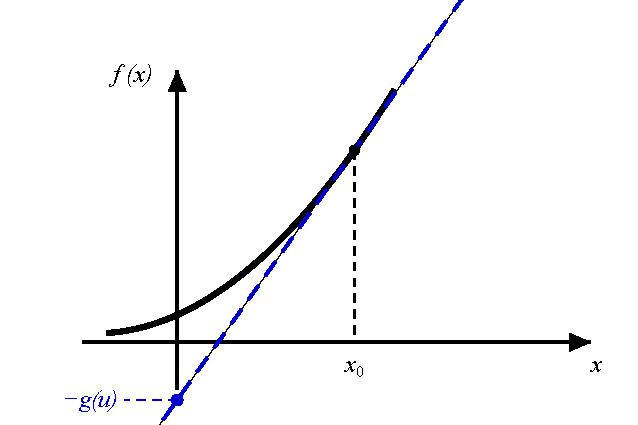
\includegraphics[width=0.58\linewidth]{Capitulo 3/Figuras/Legendre.pdf}
            \caption{Lectura geométrica de la transformada de Legendre. El valor $-g(u)$ es la ordenada en el origen de la recta tangente de pendiente $u$, de manera que describir la curva por sus tangentes contiene la misma información que describirla por sus puntos.}
            \label{fig:Legendre}
        \end{figure}

        Aplicamos la construcción al lagrangiano tomando como variable activa la velocidad generalizada y como pendiente el momento canónico \eqref{eq:MomentoCanonico}. La función transformada es la \textit{función hamiltoniana}
        \begin{equation}\label{eq:Hamiltoniano}
            H(q,p,t) \equiv \sum_{j=1}^{n}p_{j}\dot{q}_{j} - L(q,\dot{q},t),
        \end{equation}
        en la cual se entiende que todas las velocidades han sido eliminadas en favor de los momentos invirtiendo las relaciones $p_{j} = \partial L/\partial\dot{q}_{j}$. Esa inversión es posible siempre que el determinante hessiano $\det\left(\partial^{2}L/\partial\dot{q}_{j}\partial\dot{q}_{l}\right)$ no se anule, condición que se cumple para todos los lagrangianos de la forma \eqref{eq:THomogenea} porque la matriz $a_{jl}$ es definida positiva. Comparando \eqref{eq:Hamiltoniano} con \eqref{eq:hEsEnergia} vemos que el hamiltoniano es la función de energía de Jacobi expresada en las nuevas variables, y que en las condiciones allí discutidas coincide numéricamente con la energía total del sistema.

        Vamos a deducir ahora las ecuaciones de movimiento en las nuevas variables con el método de los diferenciales, que es el que hace transparente el mecanismo. Tomando el diferencial total del miembro derecho de \eqref{eq:Hamiltoniano}, tratando a $L$ como función de $(q,\dot{q},t)$,
        \begin{equation}\label{eq:DiferencialH1}
            dH = \sum_{j=1}^{n}\left(\dot{q}_{j}\,dp_{j} + p_{j}\,d\dot{q}_{j}\right)
            - \sum_{j=1}^{n}\left(\frac{\partial L}{\partial q_{j}}dq_{j} + \frac{\partial L}{\partial\dot{q}_{j}}d\dot{q}_{j}\right) - \frac{\partial L}{\partial t}dt .
        \end{equation}
        El término que contiene $d\dot{q}_{j}$ aparece dos veces con signos opuestos y coeficientes iguales, pues $\partial L/\partial\dot{q}_{j} = p_{j}$ por la definición \eqref{eq:MomentoCanonico}, de modo que
        \begin{equation}\label{eq:DiferencialH2}
            dH = \sum_{j=1}^{n}\dot{q}_{j}\,dp_{j} + \textcolor{red}{\sum_{j=1}^{n}p_{j}\,d\dot{q}_{j}} - \sum_{j=1}^{n}\frac{\partial L}{\partial q_{j}}dq_{j} - \textcolor{red}{\sum_{j=1}^{n}p_{j}\,d\dot{q}_{j}} - \frac{\partial L}{\partial t}dt,
        \end{equation}
        y los dos términos en rojo se cancelan idénticamente. Esa cancelación es el contenido entero de la transformada de Legendre: el diferencial de $H$ no contiene $d\dot{q}$, lo que demuestra que $H$ es genuinamente una función de $q$, $p$ y $t$ y no una función disfrazada de las velocidades. Queda entonces
        \begin{equation}\label{eq:DiferencialH3}
            dH = \sum_{j=1}^{n}\dot{q}_{j}\,dp_{j} - \sum_{j=1}^{n}\frac{\partial L}{\partial q_{j}}dq_{j} - \frac{\partial L}{\partial t}dt .
        \end{equation}

        Por otra parte, el diferencial de cualquier función de $(q,p,t)$ se escribe por definición como
        \begin{equation}\label{eq:DiferencialH4}
            dH = \sum_{j=1}^{n}\frac{\partial H}{\partial q_{j}}dq_{j} + \sum_{j=1}^{n}\frac{\partial H}{\partial p_{j}}dp_{j} + \frac{\partial H}{\partial t}dt .
        \end{equation}
        Como los diferenciales $dq_{j}$, $dp_{j}$ y $dt$ son independientes, la comparación término a término de \eqref{eq:DiferencialH3} y \eqref{eq:DiferencialH4} obliga a que sus coeficientes coincidan,
        \begin{equation}\label{eq:ComparacionCoef}
            \frac{\partial H}{\partial p_{j}} = \dot{q}_{j},
            \qquad
            \frac{\partial H}{\partial q_{j}} = -\frac{\partial L}{\partial q_{j}},
            \qquad
            \frac{\partial H}{\partial t} = -\frac{\partial L}{\partial t} .
        \end{equation}
        La segunda de estas relaciones se convierte en una ecuación de movimiento al invocar la ecuación de Lagrange en la forma \eqref{eq:LagrangeMomento}, que afirma $\partial L/\partial q_{j} = \dot{p}_{j}$. Reuniendo los resultados obtenemos las \textit{ecuaciones canónicas de Hamilton},
        \begin{equation}\label{eq:Hamilton}
            \boxed{\;\dot{q}_{j} = \frac{\partial H}{\partial p_{j}},
            \qquad
            \dot{p}_{j} = -\frac{\partial H}{\partial q_{j}},
            \qquad j = 1,\ldots,n .\;}
        \end{equation}

        El sistema \eqref{eq:Hamilton} consta de $2n$ ecuaciones de primer orden en lugar de $n$ de segundo orden, con lo cual el número total de constantes de integración no ha cambiado y tampoco la información física contenida. Lo que sí ha cambiado es la simetría de la descripción. En el formalismo lagrangiano las coordenadas son las protagonistas y las velocidades son cantidades derivadas de ellas; en el hamiltoniano, coordenadas y momentos aparecen en pie de igualdad, distinguidos únicamente por un signo, y esa simetría casi perfecta abre la posibilidad de transformaciones que mezclen unas con otras, cosa impensable en el lenguaje anterior. Para una partícula en un potencial, con $H = p^{2}/2m + V(x)$, las ecuaciones \eqref{eq:Hamilton} dan $\dot{x} = p/m$ y $\dot{p} = -dV/dx$, que son la definición del momento y la segunda ley de Newton escritas por separado en lugar de combinadas en una sola ecuación de segundo orden.

        Derivando $H$ respecto del tiempo a lo largo de una trayectoria y usando las propias ecuaciones canónicas, se tiene
        \begin{equation}\label{eq:ConservacionH}
            \frac{dH}{dt} = \sum_{j=1}^{n}\left(\frac{\partial H}{\partial q_{j}}\dot{q}_{j} + \frac{\partial H}{\partial p_{j}}\dot{p}_{j}\right) + \frac{\partial H}{\partial t}
            = \sum_{j=1}^{n}\left(\textcolor{red}{\frac{\partial H}{\partial q_{j}}\frac{\partial H}{\partial p_{j}}} - \textcolor{red}{\frac{\partial H}{\partial p_{j}}\frac{\partial H}{\partial q_{j}}}\right) + \frac{\partial H}{\partial t} = \frac{\partial H}{\partial t},
        \end{equation}
        donde los términos en rojo se cancelan dos a dos, recuperamos el resultado de la sección anterior en una línea: el hamiltoniano se conserva si y solo si no depende explícitamente del tiempo.

        Las $2n$ variables $(q_{1},\ldots,q_{n},p_{1},\ldots,p_{n})$ definen los puntos de una variedad de dimensión $2n$ llamada \textit{espacio de fase}, y las ecuaciones \eqref{eq:Hamilton} determinan en ella un campo vectorial cuyas curvas integrales son las trayectorias del sistema. La virtud de esta imagen es que por cada punto pasa una y solo una trayectoria, cosa que no ocurre en el espacio de configuración, donde dos movimientos distintos pueden pasar por la misma posición con velocidades diferentes; el estado dinámico queda así completamente especificado por un punto, y la evolución es un flujo.

        Ese flujo tiene una propiedad importante. Consideremos una región del espacio de fase de volumen
        \begin{equation}\label{eq:VolumenFase}
            \Omega = \int d^{n}q\,d^{n}p,
        \end{equation}
        y dejémosla evolucionar. El campo vectorial que gobierna el flujo tiene componentes $(\dot{q}_{j},\dot{p}_{j})$, y su divergencia en el espacio de fase vale
        \begin{equation}\label{eq:DivergenciaFlujo}
            \sum_{j=1}^{n}\left(\frac{\partial\dot{q}_{j}}{\partial q_{j}} + \frac{\partial\dot{p}_{j}}{\partial p_{j}}\right)
            = \sum_{j=1}^{n}\left(\frac{\partial}{\partial q_{j}}\frac{\partial H}{\partial p_{j}} - \frac{\partial}{\partial p_{j}}\frac{\partial H}{\partial q_{j}}\right)
            = \sum_{j=1}^{n}\left(\textcolor{red}{\frac{\partial^{2}H}{\partial q_{j}\partial p_{j}}} - \textcolor{red}{\frac{\partial^{2}H}{\partial p_{j}\partial q_{j}}}\right) = 0,
        \end{equation}
        donde la cancelación se debe a la igualdad de las derivadas parciales cruzadas. Un flujo de divergencia nula es incompresible, de modo que el volumen de cualquier región del espacio de fase se conserva durante la evolución, resultado conocido como \textit{teorema de Liouville} \citep{liouville1838note}. La región puede deformarse arbitrariamente, estirarse en una dirección y comprimirse en otra hasta volverse irreconocible, pero su volumen permanece constante. Este es el fundamento de la mecánica estadística clásica, y su contrapartida cuántica es la unitariedad de la evolución temporal.

    \subsection{Los corchetes de Poisson}

        La estructura algebraica del espacio de fase se expresa de manera compacta mediante la operación que Poisson introdujo en 1809 \citep{poisson1809memoire}.

        \begin{myDef}\label{def:CorchetePoisson}
            Dadas dos funciones $f(q,p,t)$ y $g(q,p,t)$ definidas sobre el espacio de fase, su \textit{corchete de Poisson} es
            \begin{equation}\label{eq:CorchetePoisson}
                \{f,g\} \equiv \sum_{j=1}^{n}\left(\frac{\partial f}{\partial q_{j}}\frac{\partial g}{\partial p_{j}} - \frac{\partial f}{\partial p_{j}}\frac{\partial g}{\partial q_{j}}\right).
            \end{equation}
        \end{myDef}

        La utilidad de esta definición se aprecia al calcular la evolución temporal de una cantidad arbitraria. Derivando $f$ a lo largo de una trayectoria y sustituyendo las ecuaciones canónicas \eqref{eq:Hamilton},
        \begin{equation}\label{eq:EvolucionPoisson}
            \frac{df}{dt} = \sum_{j=1}^{n}\left(\frac{\partial f}{\partial q_{j}}\dot{q}_{j} + \frac{\partial f}{\partial p_{j}}\dot{p}_{j}\right) + \frac{\partial f}{\partial t}
            = \sum_{j=1}^{n}\left(\frac{\partial f}{\partial q_{j}}\frac{\partial H}{\partial p_{j}} - \frac{\partial f}{\partial p_{j}}\frac{\partial H}{\partial q_{j}}\right) + \frac{\partial f}{\partial t},
        \end{equation}
        y reconociendo en el sumatorio la definición \eqref{eq:CorchetePoisson} obtenemos la \textit{ecuación de movimiento en forma de Poisson},
        \begin{equation}\label{eq:MovimientoPoisson}
            \boxed{\;\frac{df}{dt} = \{f,H\} + \frac{\partial f}{\partial t}\;}
        \end{equation}
        Toda la dinámica queda así concentrada en una sola expresión: una cantidad que no dependa explícitamente del tiempo se conserva si y solo si su corchete con el hamiltoniano se anula, y las propias ecuaciones canónicas son el caso particular $f = q_{j}$ y $f = p_{j}$, como se comprueba sustituyendo en \eqref{eq:MovimientoPoisson}.

        Las relaciones fundamentales entre las variables canónicas se obtienen directamente de la definición. Tomando $f = q_{j}$ y $g = p_{l}$, las únicas derivadas no nulas son $\partial q_{j}/\partial q_{m} = \delta_{jm}$ y $\partial p_{l}/\partial p_{m} = \delta_{lm}$, de manera que
        \begin{equation}\label{eq:CorchetesFundamentales}
            \{q_{j},p_{l}\} = \sum_{m=1}^{n}\left(\delta_{jm}\delta_{lm} - \textcolor{red}{0}\right) = \delta_{jl},
            \qquad
            \{q_{j},q_{l}\} = \{p_{j},p_{l}\} = 0 .
        \end{equation}
        El corchete de Poisson es bilineal, antisimétrico, satisface la regla de Leibniz $\{fg,h\} = f\{g,h\} + \{f,h\}g$ y cumple la identidad de Jacobi
        \begin{equation}\label{eq:IdentidadJacobi}
            \{f,\{g,h\}\} + \{g,\{h,f\}\} + \{h,\{f,g\}\} = 0,
        \end{equation}
        de modo que dota al conjunto de funciones sobre el espacio de fase de una estructura de álgebra de Lie.

        Hay una razón de fondo para habernos detenido en estas propiedades algebraicas, y es que esta es la estructura que sobrevive al paso a la mecánica cuántica. Dirac observó en 1925 que si se postula la correspondencia
        \begin{equation}\label{eq:CorrespondenciaDirac}
            \{f,g\} \;\longrightarrow\; \frac{1}{i\hbar}\left[\hat{f},\hat{g}\right],
        \end{equation}
        entonces las relaciones fundamentales \eqref{eq:CorchetesFundamentales} se convierten en las relaciones de conmutación canónicas $[\hat{q}_{j},\hat{p}_{l}] = i\hbar\delta_{jl}$, y la ecuación de movimiento \eqref{eq:MovimientoPoisson} se convierte en la ecuación de Heisenberg. En el capítulo siguiente aplicaremos exactamente este procedimiento a las amplitudes de los modos normales del campo electromagnético, y el hecho de que el álgebra resultante sea la del oscilador armónico es lo que permite hablar de fotones.

\section{Transformaciones canónicas y funciones generatrices}

    La simetría entre coordenadas y momentos en \eqref{eq:Hamilton} sugiere considerar transformaciones que mezclen unas con otras,
    \begin{equation}\label{eq:TransfCanonica}
        Q_{j} = Q_{j}(q,p,t), \qquad P_{j} = P_{j}(q,p,t),
    \end{equation}
    y preguntarse cuáles de ellas preservan la forma de las ecuaciones de movimiento. Llamaremos \textit{canónica} a una transformación tal que existe una nueva función $K(Q,P,t)$ para la cual
    \begin{equation}\label{eq:HamiltonNuevas}
        \dot{Q}_{j} = \frac{\partial K}{\partial P_{j}}, \qquad \dot{P}_{j} = -\frac{\partial K}{\partial Q_{j}} .
    \end{equation}
    El interés de estas transformaciones es puramente estratégico y es el siguiente: si consiguiéramos escoger unas variables en las cuales todas las coordenadas nuevas fuesen cíclicas, entonces todos los momentos nuevos serían constantes y el problema quedaría resuelto sin integrar nada. Llevada al extremo, esta idea conduce a la ecuación de Hamilton-Jacobi.

    La condición para que \eqref{eq:TransfCanonica} sea canónica se obtiene exigiendo que ambos juegos de variables satisfagan el principio de Hamilton. Como vimos en \eqref{eq:GaugeLagrangiano}, dos lagrangianos que difieran en una derivada total producen las mismas ecuaciones, de manera que basta con exigir
    \begin{equation}\label{eq:CondicionCanonica}
        \sum_{j=1}^{n}p_{j}\dot{q}_{j} - H = \sum_{j=1}^{n}P_{j}\dot{Q}_{j} - K + \frac{dF}{dt},
    \end{equation}
    donde $F$ es una función arbitraria llamada \textit{función generatriz}. Multiplicando por $dt$,
    \begin{equation}\label{eq:CondicionCanonicaDif}
        dF = \sum_{j=1}^{n}p_{j}\,dq_{j} - \sum_{j=1}^{n}P_{j}\,dQ_{j} + \left(K - H\right)dt .
    \end{equation}

    Si escogemos $F = F_{1}(q,Q,t)$, función de las coordenadas viejas y nuevas, su diferencial total es
    \begin{equation}\label{eq:DiferencialF1}
        dF_{1} = \sum_{j=1}^{n}\frac{\partial F_{1}}{\partial q_{j}}dq_{j} + \sum_{j=1}^{n}\frac{\partial F_{1}}{\partial Q_{j}}dQ_{j} + \frac{\partial F_{1}}{\partial t}dt,
    \end{equation}
    y comparando coeficientes con \eqref{eq:CondicionCanonicaDif}, lo que es lícito porque $dq_{j}$, $dQ_{j}$ y $dt$ son independientes, resultan las relaciones de transformación
    \begin{equation}\label{eq:RelacionesF1}
        p_{j} = \frac{\partial F_{1}}{\partial q_{j}},
        \qquad
        P_{j} = -\frac{\partial F_{1}}{\partial Q_{j}},
        \qquad
        K = H + \frac{\partial F_{1}}{\partial t} .
    \end{equation}
    La función generatriz determina así por completo la transformación: dadas $F_{1}$ y las primeras $n$ relaciones, se despejan las $Q_{j}$ en términos de $(q,p,t)$, y las segundas dan entonces los momentos nuevos.

    Las demás variantes se obtienen aplicando transformadas de Legendre a $F_{1}$ para cambiar el par de variables independientes. La que nos interesará es la de tipo dos, definida por
    \begin{equation}\label{eq:F2}
        F_{2}(q,P,t) = F_{1}(q,Q,t) + \sum_{j=1}^{n}Q_{j}P_{j},
    \end{equation}
    cuyo diferencial, usando \eqref{eq:RelacionesF1}, vale
    \begin{equation}\label{eq:DiferencialF2}
        dF_{2} = \sum_{j=1}^{n}p_{j}\,dq_{j} - \textcolor{red}{\sum_{j=1}^{n}P_{j}\,dQ_{j}} + \textcolor{red}{\sum_{j=1}^{n}P_{j}\,dQ_{j}} + \sum_{j=1}^{n}Q_{j}\,dP_{j} + \left(K-H\right)dt,
    \end{equation}
    donde los términos en rojo se cancelan, de modo que las relaciones de transformación son
    \begin{equation}\label{eq:RelacionesF2}
        p_{j} = \frac{\partial F_{2}}{\partial q_{j}},
        \qquad
        Q_{j} = \frac{\partial F_{2}}{\partial P_{j}},
        \qquad
        K = H + \frac{\partial F_{2}}{\partial t} .
    \end{equation}
    Obsérvese que $F_{2} = \sum_{j}q_{j}P_{j}$ genera la transformación identidad, lo que confirma que este tipo es el adecuado para describir transformaciones próximas a no hacer nada.

\section{La ecuación de Hamilton-Jacobi}

        Vamos a llevar ahora la estrategia al extremo, pidiendo que la transformación canónica sea tan eficaz que el nuevo hamiltoniano se anule idénticamente,
        \begin{equation}\label{eq:KCero}
            K = 0 .
        \end{equation}
        Si tal transformación existe, las ecuaciones de movimiento en las variables nuevas \eqref{eq:HamiltonNuevas} se reducen a $\dot{Q}_{j} = 0$ y $\dot{P}_{j} = 0$, de manera que las $2n$ variables nuevas son todas constantes del movimiento y el problema dinámico queda completamente resuelto: basta invertir la transformación para obtener $q_{j}(t)$.

        Usando una generatriz de tipo dos y denotándola tradicionalmente por $S$, la tercera de las relaciones \eqref{eq:RelacionesF2} junto con la exigencia \eqref{eq:KCero} da
        \begin{equation}\label{eq:HJPrevia}
            H\left(q,p,t\right) + \frac{\partial S}{\partial t} = 0,
        \end{equation}
        y sustituyendo en ella los momentos por sus expresiones $p_{j} = \partial S/\partial q_{j}$, que es la primera de las relaciones \eqref{eq:RelacionesF2}, obtenemos la \textit{ecuación de Hamilton-Jacobi},
        \begin{equation}\label{eq:HamiltonJacobi}
            \boxed{\;H\left(q_{1},\ldots,q_{n},\frac{\partial S}{\partial q_{1}},\ldots,\frac{\partial S}{\partial q_{n}},t\right) + \frac{\partial S}{\partial t} = 0 .\;}
        \end{equation}

        Se trata de una única ecuación en derivadas parciales de primer orden para la función $S(q,t)$, llamada \textit{función principal de Hamilton}. Hemos cambiado $2n$ ecuaciones diferenciales ordinarias por una sola ecuación en derivadas parciales, lo cual a primera vista parece un retroceso, y en muchos problemas concretos efectivamente lo es; pero el cambio tiene dos virtudes que lo compensan con creces. La primera es práctica: cuando la ecuación admite separación de variables, la solución se reduce a $n$ cuadraturas independientes y el problema se resuelve sin integrar ninguna ecuación diferencial acoplada. La segunda es conceptual, y es la que nos interesa aquí: la ecuación de Hamilton-Jacobi es la formulación de la mecánica clásica que más se parece a una teoría ondulatoria, porque describe la evolución de una función escalar definida sobre todo el espacio de configuración en lugar de la evolución de una trayectoria. Esa semejanza no es casual y es la que Schrödinger explotará.

        Para un sistema conservativo, en el cual $H$ no depende explícitamente del tiempo, la dependencia temporal de $S$ puede separarse escribiendo
        \begin{equation}\label{eq:SeparacionTemporal}
            S(q,t) = W(q) - Et,
        \end{equation}
        pues sustituyendo en \eqref{eq:HamiltonJacobi} se obtiene $H(q,\partial W/\partial q) = E$, ecuación que ya no contiene el tiempo y en la cual $E$ es la constante de separación, identificable con la energía. La función $W$ se llama \textit{función característica de Hamilton}.

        La función $S$ no es un artificio de cálculo: es la acción, y lo demostramos porque de ello depende toda la interpretación posterior. La derivada temporal total de $S$ a lo largo de una trayectoria efectiva del sistema vale
        \begin{equation}\label{eq:DerivadaS}
            \frac{dS}{dt} = \sum_{j=1}^{n}\frac{\partial S}{\partial q_{j}}\dot{q}_{j} + \frac{\partial S}{\partial t},
        \end{equation}
        y sustituyamos las dos identificaciones que la propia construcción nos ha dado, a saber $\partial S/\partial q_{j} = p_{j}$ y, por \eqref{eq:HJPrevia}, $\partial S/\partial t = -H$,
        \begin{equation}\label{eq:DerivadaS2}
            \frac{dS}{dt} = \sum_{j=1}^{n}p_{j}\dot{q}_{j} - H = L,
        \end{equation}
        donde el último paso es la definición \eqref{eq:Hamiltoniano} del hamiltoniano despejada para $L$. Integrando entre dos instantes,
        \begin{equation}\label{eq:SEsAccion}
            S = \int L\,dt + \text{constante},
        \end{equation}
        de manera que la función principal de Hamilton es la acción evaluada sobre la trayectoria efectiva del sistema, considerada como función del punto final y del instante final. Esta es una diferencia sutil pero decisiva respecto de la acción \eqref{eq:Accion} de la sección anterior: allí $S$ era un funcional definido sobre todos los caminos imaginables con extremos fijos, mientras que aquí es una función ordinaria de las coordenadas finales, obtenida al evaluar la acción únicamente sobre el camino clásico que llega a ese punto.

        \begin{figure}[htbp]
            \centering
            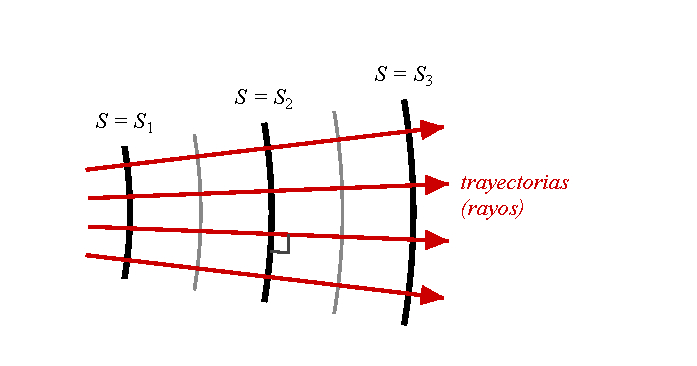
\includegraphics[width=0.62\linewidth]{Capitulo 3/Figuras/FrentesAccion.pdf}
            \caption{Superficies de acción constante y trayectorias mecánicas. El momento es el gradiente de $S$, de modo que las trayectorias cortan perpendicularmente a los frentes, exactamente como los rayos luminosos cortan a los frentes de onda.}
            \label{fig:FrentesAccion}
        \end{figure}

        La relación $p_{j} = \partial S/\partial q_{j}$ admite entonces una lectura geométrica que es el corazón de la analogía óptico-mecánica. Las superficies $S(q,t) = \text{constante}$ forman una familia que barre el espacio de configuración a medida que transcurre el tiempo, y el gradiente de $S$, que es perpendicular a esas superficies, es el momento de la partícula. \textbf{Las trayectorias mecánicas son, por tanto, las curvas ortogonales a las superficies de acción constante}, exactamente como los rayos luminosos son las curvas ortogonales a los frentes de onda. La sección siguiente hace explícita esa correspondencia.

        Ilustremos el método en el caso más simple posible, donde todo puede calcularse hasta el final. Para una partícula libre en una dimensión el hamiltoniano es $H = p^{2}/2m$, y la ecuación \eqref{eq:HamiltonJacobi} se escribe
        \begin{equation}\label{eq:HJLibre}
            \frac{1}{2m}\left(\frac{\partial S}{\partial x}\right)^{2} + \frac{\partial S}{\partial t} = 0 .
        \end{equation}
        Separando la dependencia temporal según \eqref{eq:SeparacionTemporal} con $S = W(x) - Et$, y sustituyendo,
        \begin{equation}\label{eq:HJLibre2}
            \frac{1}{2m}\left(\frac{dW}{dx}\right)^{2} = E
            \qquad\Longrightarrow\qquad
            \frac{dW}{dx} = \sqrt{2mE},
        \end{equation}
        que se integra de inmediato dando $W = \sqrt{2mE}\,x$, de modo que
        \begin{equation}\label{eq:SLibre}
            S(x,t) = \sqrt{2mE}\,x - Et .
        \end{equation}
        Las superficies de acción constante son en este caso planos perpendiculares al eje, y avanzan con velocidad
        \begin{equation}\label{eq:VelocidadFrente}
            u = \frac{E}{\sqrt{2mE}} = \sqrt{\frac{E}{2m}} = \frac{v}{2},
        \end{equation}
        donde $v = \sqrt{2E/m}$ es la velocidad de la partícula. El resultado es contraintuitivo: los frentes de acción constante se mueven a la mitad de la velocidad de la partícula, de manera que la analogía con una onda, si ha de mantenerse, exige que la partícula corresponda no a la velocidad de fase de esa onda sino a algo distinto. Volveremos sobre esta discrepancia al discutir la velocidad de grupo, porque es exactamente el punto en el que de Broglie y Schrödinger tuvieron que ser cuidadosos.

        Para completar el ejemplo, la constante de integración $E$ hace el papel del momento nuevo $P$, y la coordenada nueva conjugada se obtiene de la segunda relación \eqref{eq:RelacionesF2},
        \begin{equation}\label{eq:QLibre}
            Q = \frac{\partial S}{\partial E} = \sqrt{\frac{m}{2E}}\,x - t = \text{constante},
        \end{equation}
        de donde, despejando, $x = \sqrt{2E/m}\,(t + Q) = v\,t + x_{0}$, que es el movimiento rectilíneo uniforme esperado. El método ha producido la solución sin integrar ninguna ecuación de movimiento.

    \subsection{Ejemplo: el oscilador armónico y su acción clásica}

        El segundo ejemplo es el que necesitaremos literalmente más adelante, porque el campo electromagnético cuantizado es una colección de osciladores armónicos y la propagación de los fotones se describirá mediante el propagador de un oscilador. Calcularemos aquí la acción clásica del oscilador como función de sus extremos, que es el ingrediente central de ese propagador.

        El lagrangiano y el hamiltoniano de un oscilador de masa $m$ y frecuencia $\omega$ son
        \begin{equation}\label{eq:LagrangianoOsc}
            L = \frac{1}{2}m\dot{q}^{2} - \frac{1}{2}m\omega^{2}q^{2},
            \qquad
            H = \frac{p^{2}}{2m} + \frac{1}{2}m\omega^{2}q^{2},
        \end{equation}
        y la ecuación de movimiento que se sigue de \eqref{eq:EulerLagrange2} es $\ddot{q} + \omega^{2}q = 0$, cuya solución general escribimos en la forma
        \begin{equation}\label{eq:SolucionOsc}
            q(s) = A\cos\omega s + B\sin\omega s .
        \end{equation}
        Impongamos las condiciones de contorno propias de un problema variacional, es decir, valores prescritos en los dos extremos del intervalo temporal, $q(0) = q_{I}$ y $q(t) = q_{F}$. La primera da inmediatamente $A = q_{I}$, y la segunda
        \begin{equation}\label{eq:CondicionB}
            q_{F} = q_{I}\cos\omega t + B\sin\omega t
            \qquad\Longrightarrow\qquad
            B = \frac{q_{F} - q_{I}\cos\omega t}{\sin\omega t},
        \end{equation}
        expresión que exige $\sin\omega t \neq 0$, condición cuyo significado físico discutiremos al final. La trayectoria clásica que une ambos puntos es por tanto
        \begin{equation}\label{eq:TrayectoriaOsc}
            q_{\mathrm{cl}}(s) = q_{I}\cos\omega s + \frac{q_{F} - q_{I}\cos\omega t}{\sin\omega t}\,\sin\omega s .
        \end{equation}

        Para evaluar la acción sobre esta trayectoria simplificamos primero el integrando mediante una integración por partes, lo que evita tener que elevar al cuadrado la expresión anterior. Partimos de
        \begin{equation}\label{eq:AccionOsc1}
            S_{\mathrm{cl}} = \int_{0}^{t}\left(\frac{1}{2}m\dot{q}^{2} - \frac{1}{2}m\omega^{2}q^{2}\right)ds,
        \end{equation}
        y transformamos el término cinético escribiendo $\dot{q}^{2} = \frac{d}{ds}(q\dot{q}) - q\ddot{q}$, identidad que no es más que la regla del producto reordenada,
        \begin{equation}\label{eq:AccionOsc2}
            S_{\mathrm{cl}} = \frac{m}{2}\left[q\dot{q}\right]_{0}^{t} - \frac{m}{2}\int_{0}^{t} q\left(\ddot{q} + \textcolor{blue}{\omega^{2}q}\right)ds,
        \end{equation}
        donde el término en azul se ha agrupado deliberadamente con $\ddot{q}$ para formar el miembro izquierdo de la ecuación de movimiento. Como la trayectoria es clásica, ese paréntesis se anula idénticamente y la integral desaparece por completo,
        \begin{equation}\label{eq:AccionOscFrontera}
            S_{\mathrm{cl}} = \frac{m}{2}\left[q_{\mathrm{cl}}(t)\dot{q}_{\mathrm{cl}}(t) - q_{\mathrm{cl}}(0)\dot{q}_{\mathrm{cl}}(0)\right].
        \end{equation}
        El resultado no es privativo del oscilador. La acción clásica de cualquier sistema cuadrático se reduce a un término de frontera, lo cual explica por qué el oscilador armónico y la partícula libre son los únicos sistemas cuyo propagador puede escribirse en forma cerrada elemental.

        Solo resta evaluar las velocidades en los extremos. Derivando \eqref{eq:TrayectoriaOsc},
        \begin{equation}\label{eq:VelocidadOsc}
            \dot{q}_{\mathrm{cl}}(s) = -q_{I}\omega\sin\omega s + \omega\,\frac{q_{F}-q_{I}\cos\omega t}{\sin\omega t}\cos\omega s,
        \end{equation}
        de donde, en $s=0$, donde $\sin 0 = 0$ y $\cos 0 = 1$,
        \begin{equation}\label{eq:VelocidadInicial}
            \dot{q}_{\mathrm{cl}}(0) = \omega\,\frac{q_{F}-q_{I}\cos\omega t}{\sin\omega t},
        \end{equation}
        y en $s=t$,
        \begin{equation}\label{eq:VelocidadFinal}
            \dot{q}_{\mathrm{cl}}(t) = -q_{I}\omega\sin\omega t + \omega\,\frac{\left(q_{F}-q_{I}\cos\omega t\right)\cos\omega t}{\sin\omega t}
            = \omega\,\frac{-q_{I}\sin^{2}\omega t + q_{F}\cos\omega t - q_{I}\cos^{2}\omega t}{\sin\omega t},
        \end{equation}
        donde hemos puesto todo sobre el denominador común $\sin\omega t$. Los dos términos en $q_{I}$ se combinan mediante la identidad pitagórica $\sin^{2}\omega t + \cos^{2}\omega t = 1$,
        \begin{equation}\label{eq:VelocidadFinal2}
            \dot{q}_{\mathrm{cl}}(t) = \omega\,\frac{q_{F}\cos\omega t - q_{I}}{\sin\omega t} .
        \end{equation}

        Sustituyendo \eqref{eq:VelocidadInicial} y \eqref{eq:VelocidadFinal2} en \eqref{eq:AccionOscFrontera},
        \begin{equation}\label{eq:AccionOsc3}
            S_{\mathrm{cl}} = \frac{m\omega}{2\sin\omega t}\left[q_{F}\left(q_{F}\cos\omega t - q_{I}\right) - q_{I}\left(q_{F} - q_{I}\cos\omega t\right)\right],
        \end{equation}
        y desarrollando los dos productos del corchete,
        \begin{equation}\label{eq:AccionOsc4}
            S_{\mathrm{cl}} = \frac{m\omega}{2\sin\omega t}\left[q_{F}^{2}\cos\omega t - q_{I}q_{F} - q_{I}q_{F} + q_{I}^{2}\cos\omega t\right],
        \end{equation}
        de manera que los dos términos cruzados, que son idénticos, se suman y obtenemos finalmente
        \begin{equation}\label{eq:AccionOscilador}
            \boxed{\;S_{\mathrm{cl}}(q_{F},t;q_{I},0) = \frac{m\omega}{2\sin\omega t}\left[\left(q_{I}^{2}+q_{F}^{2}\right)\cos\omega t - 2q_{I}q_{F}\right].\;}
        \end{equation}

        Merece la pena detenerse en esta expresión, porque es exactamente el exponente que aparecerá en el propagador del campo electromagnético cuantizado. Dividiendo numerador y denominador por $\sin\omega t$ el resultado puede escribirse de manera equivalente como
        \begin{equation}\label{eq:AccionOsciladorCot}
            S_{\mathrm{cl}} = \frac{m\omega}{2}\left[\left(q_{I}^{2}+q_{F}^{2}\right)\cot\omega t - \frac{2q_{I}q_{F}}{\sin\omega t}\right],
        \end{equation}
        y esta es, salvo el factor de masa, la combinación de una cotangente multiplicando a la suma de cuadrados y de una cosecante multiplicando al producto cruzado que reconoceremos en el núcleo de la transformada de Fourier fraccionaria y en la integral de difracción de Fresnel. La estructura matemática que conecta la propagación de la luz clásica con la evolución de un fotón está contenida, en germen, en esta expresión puramente mecánica.

        Vale la pena ver qué ocurre cuando $\omega t$ se aproxima a un múltiplo entero de $\pi$. El denominador $\sin\omega t$ se anula y la acción diverge, salvo para pares de puntos particulares; físicamente, tras medio período todas las trayectorias que parten de $q_{I}$ vuelven a converger en el mismo punto, de manera que el problema de contorno deja de tener solución única. Estos instantes se llaman \textit{puntos conjugados} o \textit{cáusticas}, y la divergencia de la acción en ellos es el análogo mecánico exacto del foco de un sistema óptico, donde la aproximación de rayos también deja de ser válida. En el lenguaje del capítulo dedicado a la difracción, un punto conjugado es aquel en el cual la fase estacionaria degenera y el cálculo asintótico debe refinarse.

    \subsection{La analogía óptico-mecánica de Hamilton}

        Estamos ya en condiciones de establecer con precisión la correspondencia que Hamilton descubrió en 1834 y que constituye el puente hacia la mecánica ondulatoria.

        En óptica geométrica, el principio de Fermat establece que un rayo luminoso entre dos puntos recorre un camino de longitud óptica estacionaria,
        \begin{equation}\label{eq:Fermat}
            \delta\int_{A}^{B} n(\mathbf{r})\,dl = 0,
        \end{equation}
        donde $n$ es el índice de refracción. En mecánica, el principio de Maupertuis, que se obtiene del de Hamilton restringiéndose a variaciones que conservan la energía, establece que la trayectoria de una partícula satisface
        \begin{equation}\label{eq:Maupertuis}
            \delta\int_{A}^{B} p\,dl = 0,
            \qquad
            p = \sqrt{2m\left[E - V(\mathbf{r})\right]} .
        \end{equation}
        Las dos expresiones son formalmente idénticas, y la correspondencia entre ellas exige identificar
        \begin{equation}\label{eq:DiccionarioHamilton}
            n(\mathbf{r}) \;\longleftrightarrow\; \sqrt{2m\left[E-V(\mathbf{r})\right]} = p,
        \end{equation}
        es decir, el índice de refracción del medio mecánico es el momento de la partícula. Un potencial atractivo actúa sobre las trayectorias exactamente como un medio de índice creciente actúa sobre los rayos, y la refracción de una partícula al atravesar un escalón de potencial obedece una ley de Snell con los momentos en lugar de los índices.

        La correspondencia se extiende al nivel de las funciones. En óptica, la fase de la onda define la \textit{eikonal} $\mathcal{L}(\mathbf{r})$ mediante $\mathcal{E} \sim \exp\left[ik_{0}\mathcal{L}\right]$, y los frentes de onda son sus superficies de nivel, mientras que en mecánica es la función característica $W$ la que juega ese papel. Al sustituir la forma eikonal en la ecuación de Helmholtz y quedarse con el término dominante en el límite de longitud de onda corta se obtiene la \textit{ecuación de la eikonal},
        \begin{equation}\label{eq:Eikonal}
            \left\|\nabla\mathcal{L}\right\|^{2} = n^{2}(\mathbf{r}),
        \end{equation}
        y al sustituir $p = \nabla W$ en $H = E$ se obtiene la ecuación de Hamilton-Jacobi independiente del tiempo,
        \begin{equation}\label{eq:HJIndependiente}
            \left\|\nabla W\right\|^{2} = 2m\left[E - V(\mathbf{r})\right] .
        \end{equation}
        Las dos ecuaciones tienen la misma forma, y el diccionario \eqref{eq:DiccionarioHamilton} las transforma una en otra.

        Hamilton se detuvo aquí, y la razón es comprensible: en su época no existía ningún indicio experimental de que la mecánica clásica fuese el límite de otra cosa, de manera que la analogía era una elegancia matemática sin consecuencias. La pregunta que Hamilton no hizo, y que noventa años después haría de Broglie, es la siguiente: si la mecánica clásica es a la mecánica verdadera lo que la óptica geométrica es a la óptica ondulatoria, entonces debe existir una ecuación de ondas subyacente cuya aproximación eikonal sea la ecuación de Hamilton-Jacobi, y esa ecuación describiría el comportamiento de la materia allí donde la aproximación de rayos falla. La sección siguiente reconstruye el camino que llevó de esa pregunta a la ecuación de Schrödinger.

\section{De la ecuación de Hamilton-Jacobi a la ecuación de Schrödinger}

        En su tesis doctoral de 1924 Louis de Broglie propuso que la dualidad que Einstein había establecido para la luz debía extenderse a la materia, de manera que a toda partícula de momento $p$ le corresponde una onda de longitud
        \begin{equation}\label{eq:deBroglie}
            \lambda = \frac{h}{p},
            \qquad\text{equivalentemente}\qquad
            k = \frac{2\pi}{\lambda} = \frac{p}{\hbar},
        \end{equation}
        y a toda energía $E$ una frecuencia
        \begin{equation}\label{eq:PlanckEinstein}
            \omega = \frac{E}{\hbar} .
        \end{equation}
        Estas dos relaciones bastan para cerrar el diccionario de Hamilton, porque convierten la correspondencia formal entre la eikonal y la función característica en una afirmación cuantitativa sobre una onda física.

        Comprobémoslo. Si la fase de esa onda ha de ser proporcional a la función principal de Hamilton, como exige la identificación de los frentes de onda con las superficies de acción constante, entonces escribimos
        \begin{equation}\label{eq:FaseEsAccion}
            \Phi(\mathbf{r},t) = \frac{S(\mathbf{r},t)}{\hbar} = \frac{W(\mathbf{r}) - Et}{\hbar},
        \end{equation}
        y las dos relaciones de de Broglie se siguen de inmediato: el gradiente de la fase es $\nabla\Phi = \nabla W/\hbar = \mathbf{p}/\hbar$, que es el vector de onda, y la derivada temporal es $\partial\Phi/\partial t = -E/\hbar$, que es la frecuencia angular con el signo convencional. La constante $\hbar$ entra en la teoría únicamente como el factor de conversión entre la acción y la fase, y esa es toda su función: sin ella, la exponencial de una acción no tendría sentido dimensional.

        Podemos aclarar de una vez la dificultad que mencionamos al tratar la partícula libre, porque es la que estuvo a punto de descarrilar la construcción. La velocidad con que avanzan los frentes de fase constante es
        \begin{equation}\label{eq:VelocidadFase}
            u = \frac{\omega}{k} = \frac{E/\hbar}{p/\hbar} = \frac{E}{p} = \frac{E}{\sqrt{2m\left[E-V\right]}},
        \end{equation}
        que para una partícula libre no relativista vale $u = (p^{2}/2m)/p = v/2$, es decir, la mitad de la velocidad de la partícula, tal como habíamos obtenido en \eqref{eq:VelocidadFrente}. Si la partícula fuese la onda, la contradicción sería fatal. La solución está en que una partícula localizada no corresponde a una onda monocromática sino a un paquete construido superponiendo un intervalo estrecho de frecuencias, y un paquete no viaja con la velocidad de fase sino con la \textit{velocidad de grupo},
        \begin{equation}\label{eq:VelocidadGrupo}
            v_{g} = \frac{d\omega}{dk} = \frac{d(E/\hbar)}{d(p/\hbar)} = \frac{dE}{dp} = \frac{d}{dp}\left(\frac{p^{2}}{2m}\right) = \frac{p}{m} = v,
        \end{equation}
        que sí coincide con la velocidad clásica. Obsérvese además que la velocidad de fase \eqref{eq:VelocidadFase} depende del origen desde el cual se mida la energía, pues sumar una constante al potencial cambia $E$ y por tanto cambia $u$, mientras que la velocidad de grupo \eqref{eq:VelocidadGrupo}, al ser una derivada, no se ve afectada. La velocidad de fase no es una cantidad física y la velocidad de grupo sí lo es, y esta observación, que hoy resulta rutinaria en el estudio de la coherencia y de la propagación de pulsos, fue en 1924 el argumento decisivo que permitió a de Broglie sostener su hipótesis frente a la objeción más obvia que se le podía hacer.

        Disponemos ya de todos los elementos para ejecutar el programa. La lógica es la siguiente: si la mecánica clásica es el límite de rayos de una teoría ondulatoria, escribamos la ecuación de ondas más simple posible, la ecuación de onda clásica, dotémosla de la velocidad de fase que la ecuación de Hamilton-Jacobi prescribe, e impongamos las relaciones de de Broglie. Veremos que ese procedimiento produce, sin ningún ingrediente adicional, la ecuación de Schrödinger.

        Partimos entonces de la ecuación de onda clásica para una función escalar $\Psi(\mathbf{r},t)$ que se propaga en un medio con velocidad de fase $u(\mathbf{r})$ dependiente de la posición,
        \begin{equation}\label{eq:OndaClasica}
            \nabla^{2}\Psi(\mathbf{r},t) - \frac{1}{u^{2}(\mathbf{r})}\frac{\partial^{2}\Psi(\mathbf{r},t)}{\partial t^{2}} = 0,
        \end{equation}
        que es exactamente la ecuación con la que iniciamos el estudio de la difracción escalar en \ref{Sec:Diffraction}, allí con $u = c/n$ y aquí con la velocidad de fase mecánica \eqref{eq:VelocidadFase}. La analogía óptico-mecánica no es aquí una metáfora: estamos usando literalmente la misma ecuación con otro índice de refracción.

        Busquemos soluciones monocromáticas, es decir, de frecuencia bien definida, separando la dependencia temporal en la forma
        \begin{equation}\label{eq:SeparacionMonocromatica}
            \Psi(\mathbf{r},t) = \psi(\mathbf{r})\,e^{-i\omega t} .
        \end{equation}
        Derivando dos veces respecto del tiempo, cada derivada baja un factor $-i\omega$,
        \begin{equation}\label{eq:SegundaDerivadaTemporal}
            \frac{\partial^{2}\Psi}{\partial t^{2}} = \left(-i\omega\right)^{2}\psi(\mathbf{r})e^{-i\omega t} = -\omega^{2}\,\psi(\mathbf{r})\,e^{-i\omega t},
        \end{equation}
        y sustituyendo en \eqref{eq:OndaClasica},
        \begin{equation}\label{eq:HelmholtzPaso}
            \left[\nabla^{2}\psi(\mathbf{r}) + \frac{\omega^{2}}{u^{2}(\mathbf{r})}\psi(\mathbf{r})\right]\textcolor{red}{e^{-i\omega t}} = 0 .
        \end{equation}
        La exponencial marcada en rojo nunca se anula, de modo que puede dividirse la ecuación por ella, y queda la ecuación de Helmholtz
        \begin{equation}\label{eq:HelmholtzMecanico}
            \nabla^{2}\psi + \frac{\omega^{2}}{u^{2}}\psi = 0 .
        \end{equation}
        Este es el mismo paso que dimos al deducir la ecuación de Helmholtz óptica, y hasta aquí no hemos usado ninguna hipótesis cuántica: \eqref{eq:HelmholtzMecanico} es física ondulatoria del siglo XIX.

        El ingrediente cuántico entra ahora, y entra por una sola puerta. Sustituimos en el coeficiente $\omega^{2}/u^{2}$ la frecuencia dada por la relación de Planck y Einstein \eqref{eq:PlanckEinstein} y la velocidad de fase dada por Hamilton-Jacobi \eqref{eq:VelocidadFase},
        \begin{equation}\label{eq:CoeficienteSustituido}
            \frac{\omega^{2}}{u^{2}} = \frac{\left(E/\hbar\right)^{2}}{\left(E/p\right)^{2}}
            = \frac{E^{2}}{\hbar^{2}}\cdot\frac{p^{2}}{E^{2}}
            = \frac{p^{2}}{\hbar^{2}},
        \end{equation}
        donde el cuadrado de la energía se cancela por completo entre el numerador y el denominador. Este detalle es importante: la energía total desaparece del coeficiente y solo sobrevive el momento, que es precisamente la cantidad que la relación de de Broglie \eqref{eq:deBroglie} conecta con la longitud de onda, de modo que el coeficiente de \eqref{eq:HelmholtzMecanico} es simplemente $k^{2} = (2\pi/\lambda)^{2}$, tal y como ocurre en la óptica.

        Sustituyendo ahora el momento mecánico $p^{2} = 2m\left[E - V(\mathbf{r})\right]$, que es la relación que define la velocidad de fase en \eqref{eq:VelocidadFase} y que proviene de la ecuación de Hamilton-Jacobi independiente del tiempo \eqref{eq:HJIndependiente},
        \begin{equation}\label{eq:SchrodingerPaso1}
            \nabla^{2}\psi + \frac{2m}{\hbar^{2}}\left[E - V(\mathbf{r})\right]\psi = 0 .
        \end{equation}
        Multiplicando por $-\hbar^{2}/2m$ y reordenando los términos de manera que la energía quede aislada a la derecha,
        \begin{equation}\label{eq:SchrodingerEstacionaria}
            \boxed{\;-\frac{\hbar^{2}}{2m}\nabla^{2}\psi(\mathbf{r}) + V(\mathbf{r})\,\psi(\mathbf{r}) = E\,\psi(\mathbf{r}),\;}
        \end{equation}
        que es la \textit{ecuación de Schrödinger independiente del tiempo}, tal como apareció en la primera comunicación de enero de 1926 \citep{schrodinger1926quantisierung}.

        Vale la pena mirar lo ocurrido. No hemos postulado nada que no estuviera ya en la mesa: la ecuación de onda clásica es del siglo XVIII, la velocidad de fase la fija la ecuación de Hamilton-Jacobi del siglo XIX, y las dos únicas relaciones nuevas son $E = \hbar\omega$ y $p = \hbar k$. El contenido físico de \eqref{eq:SchrodingerEstacionaria} tampoco está en su forma, que es la de una ecuación de Helmholtz con índice de refracción variable, sino en las condiciones de contorno: exigir que $\psi$ sea finita, univaluada y de cuadrado integrable en todo el espacio selecciona únicamente ciertos valores de $E$, exactamente igual que exigir que una cuerda esté sujeta en sus dos extremos selecciona únicamente ciertas frecuencias de vibración. La cuantización de la energía deja de ser un postulado ad hoc, como lo era en el modelo de Bohr, y se convierte en un problema de valores propios de una ecuación diferencial, que es precisamente lo que anuncia el título de la memoria de Schrödinger, \textit{Quantisierung als Eigenwertproblem}, la cuantización como problema de valores propios.

    \subsection{El camino que siguió Schrödinger: la sustitución exponencial}

        La reconstrucción anterior es la que se presenta habitualmente y es la que Schrödinger desarrolló con detalle en su segunda comunicación \citep{schrodinger1926quantisierungII}, pero no es la que aparece en la primera. El razonamiento original es más breve y más audaz, y merece reproducirse porque en él la ecuación de Hamilton-Jacobi no es un ingrediente auxiliar sino el punto de partida literal.

        Schrödinger parte de la ecuación de Hamilton-Jacobi independiente del tiempo para un sistema conservativo, que escribimos en la forma
        \begin{equation}\label{eq:HJPartida}
            \frac{1}{2m}\left\|\nabla W\right\|^{2} + V(\mathbf{r}) = E,
        \end{equation}
        e introduce una nueva función incógnita $\psi$ mediante la sustitución
        \begin{equation}\label{eq:SustitucionLog}
            W = K\ln\psi,
        \end{equation}
        donde $K$ es por el momento una constante con dimensiones de acción, cuyo valor se fijará al final. La motivación de esta sustitución es que convierte la relación multiplicativa entre las funciones de onda de subsistemas independientes en la relación aditiva que la acción satisface, pues la acción de dos sistemas independientes se suma mientras que sus amplitudes se multiplican, y el logaritmo es la única función que convierte productos en sumas.

        El gradiente de \eqref{eq:SustitucionLog} se obtiene con la regla de la cadena,
        \begin{equation}\label{eq:GradienteLog}
            \nabla W = K\,\frac{\nabla\psi}{\psi},
        \end{equation}
        y sustituyámoslo en \eqref{eq:HJPartida},
        \begin{equation}\label{eq:HJSustituida}
            \frac{K^{2}}{2m}\frac{\left\|\nabla\psi\right\|^{2}}{\psi^{2}} + V = E .
        \end{equation}
        Multiplicando por $2m\psi^{2}$ y pasando todo a un miembro obtenemos una expresión polinómica, libre ya de denominadores,
        \begin{equation}\label{eq:HJPolinomica}
            K^{2}\left\|\nabla\psi\right\|^{2} - 2m\left[E - V\right]\psi^{2} = 0 .
        \end{equation}

        Aquí se produce el paso decisivo, y también el más discutido. Schrödinger no intenta resolver \eqref{eq:HJPolinomica}, que sigue siendo una ecuación de Hamilton-Jacobi disfrazada y por tanto sigue describiendo mecánica clásica. Lo que hace es sustituir la exigencia de que la expresión se anule punto a punto por la exigencia, mucho más débil, de que su integral sobre todo el espacio sea estacionaria,
        \begin{equation}\label{eq:FuncionalSchrodinger}
            \delta J[\psi] = 0,
            \qquad
            J[\psi] = \int_{\mathbb{R}^{3}}\left\{K^{2}\left\|\nabla\psi\right\|^{2} - 2m\left[E - V(\mathbf{r})\right]\psi^{2}\right\}d^{3}r .
        \end{equation}
        La justificación que Schrödinger ofrece es de analogía: así como el principio de Fermat, que exige la estacionariedad de una integral, da la óptica geométrica correcta pero solo describe rayos, y la descripción completa exige una ecuación de ondas, del mismo modo la mecánica de trayectorias debe ceder el paso a un principio variacional sobre un campo definido en todo el espacio. Es un salto, y él mismo lo reconoce; su validación es que funciona.

        La variación indicada en \eqref{eq:FuncionalSchrodinger} es un ejercicio del cálculo de variaciones idéntico al de la sección anterior salvo que ahora la variable independiente es el punto del espacio y no el tiempo. Variando $\psi\rightarrow\psi + \delta\psi$ y quedándonos con el primer orden,
        \begin{equation}\label{eq:VariacionJ}
            \delta J = \int_{\mathbb{R}^{3}}\left\{2K^{2}\,\nabla\psi\cdot\nabla\delta\psi - 4m\left[E-V\right]\psi\,\delta\psi\right\}d^{3}r,
        \end{equation}
        donde el factor dos del primer término proviene de derivar un cuadrado y el factor cuatro del segundo de derivar el otro cuadrado multiplicado por el dos que ya estaba. Para poder factorizar $\delta\psi$ hay que quitarle el gradiente al primer término, y eso se consigue con la identidad vectorial
        \begin{equation}\label{eq:IdentidadDivergencia}
            \nabla\cdot\left(\delta\psi\,\nabla\psi\right) = \nabla\delta\psi\cdot\nabla\psi + \delta\psi\,\nabla^{2}\psi
            \qquad\Longrightarrow\qquad
            \nabla\psi\cdot\nabla\delta\psi = \nabla\cdot\left(\delta\psi\,\nabla\psi\right) - \delta\psi\,\nabla^{2}\psi,
        \end{equation}
        que es la versión tridimensional de la integración por partes. Al integrar el primer término del miembro derecho sobre todo el espacio, el teorema de la divergencia lo convierte en un flujo a través de una superficie en el infinito,
        \begin{equation}\label{eq:FlujoInfinito}
            \int_{\mathbb{R}^{3}}\nabla\cdot\left(\delta\psi\,\nabla\psi\right)d^{3}r
            = \textcolor{red}{\oint_{\Sigma_{\infty}}\delta\psi\,\nabla\psi\cdot d\boldsymbol{\sigma}} = 0,
        \end{equation}
        que se anula porque exigimos que $\psi$ y sus variaciones decaigan suficientemente rápido para que la función sea de cuadrado integrable. Este es el mismo mecanismo que en \eqref{eq:TerminoFrontera} eliminaba el término de frontera temporal, y desempeña aquí el mismo papel.

        Sustituyendo \eqref{eq:IdentidadDivergencia} y \eqref{eq:FlujoInfinito} en \eqref{eq:VariacionJ} y factorizando,
        \begin{equation}\label{eq:VariacionJFactorizada}
            \delta J = -2\int_{\mathbb{R}^{3}}\left\{K^{2}\nabla^{2}\psi + 2m\left[E-V\right]\psi\right\}\delta\psi\;d^{3}r = 0 .
        \end{equation}
        Como $\delta\psi$ es arbitraria, el lema fundamental \ref{teo:LemaFundamental}, aplicado ahora en tres dimensiones con idéntica demostración, obliga a que se anule la llave,
        \begin{equation}\label{eq:SchrodingerConK}
            K^{2}\nabla^{2}\psi + 2m\left[E - V(\mathbf{r})\right]\psi = 0 .
        \end{equation}

        Comparando \eqref{eq:SchrodingerConK} con \eqref{eq:SchrodingerPaso1} vemos que ambas coinciden exactamente si y solo si
        \begin{equation}\label{eq:FijarK}
            K = \hbar = \frac{h}{2\pi} .
        \end{equation}
        Schrödinger no disponía de este argumento y fijó la constante de otro modo, que es mucho más convincente: resolvió \eqref{eq:SchrodingerConK} para el potencial coulombiano del átomo de hidrógeno, encontró que las soluciones aceptables existen únicamente para el conjunto discreto de energías
        \begin{equation}\label{eq:Balmer}
            E_{n} = -\frac{me^{4}}{2\left(4\pi\epsilon_{0}\right)^{2}K^{2}n^{2}}, \qquad n = 1,2,3,\ldots,
        \end{equation}
        y observó que la elección $K = h/2\pi$ reproduce exactamente la fórmula de Balmer y el valor medido de la constante de Rydberg. La constante de Planck no fue introducida en la mecánica ondulatoria como un postulado sino ajustada para reproducir un espectro medido, y el hecho de que el mismo valor sirva después para todos los demás sistemas es la evidencia de que la teoría es correcta.

        La ecuación \eqref{eq:SchrodingerEstacionaria} contiene la energía como parámetro, de manera que describe estados de energía definida y no permite superponerlos, pues una combinación lineal de soluciones con energías distintas no satisface ninguna de las dos ecuaciones. Para obtener una ecuación válida para estados arbitrarios hay que eliminar $E$, y el procedimiento es directo.

        Para un estado de energía definida, la dependencia temporal es la de \eqref{eq:SeparacionMonocromatica} con $\omega = E/\hbar$,
        \begin{equation}\label{eq:EstadoEstacionario}
            \Psi(\mathbf{r},t) = \psi(\mathbf{r})\,e^{-iEt/\hbar},
        \end{equation}
        y derivando respecto del tiempo se obtiene una identidad notable,
        \begin{equation}\label{eq:EnergiaComoOperador}
            i\hbar\frac{\partial\Psi}{\partial t} = i\hbar\left(-\frac{iE}{\hbar}\right)\psi\,e^{-iEt/\hbar} = E\,\Psi,
        \end{equation}
        donde hemos usado $i\cdot(-i) = 1$. La energía, que era un número, aparece así como el resultado de aplicar el operador $i\hbar\,\partial/\partial t$ a la función de onda. Sustituyendo esta identificación en el miembro derecho de \eqref{eq:SchrodingerEstacionaria}, y escribiendo la función completa $\Psi$ en lugar de su parte espacial, resulta la \textit{ecuación de Schrödinger dependiente del tiempo},
        \begin{equation}\label{eq:SchrodingerTemporal}
            \boxed{\;i\hbar\frac{\partial\Psi(\mathbf{r},t)}{\partial t} = -\frac{\hbar^{2}}{2m}\nabla^{2}\Psi(\mathbf{r},t) + V(\mathbf{r})\,\Psi(\mathbf{r},t) .\;}
        \end{equation}

        La ecuación así obtenida es lineal, de manera que ahora sí admite superposiciones arbitrarias, y es de primer orden en el tiempo, lo cual constituye la diferencia estructural más profunda respecto de la ecuación de onda clásica \eqref{eq:OndaClasica} de la que partimos. ¿Por qué era inevitable esa diferencia? La ecuación clásica es de segundo orden en el tiempo porque la relación de dispersión de una onda ordinaria es $\omega^{2} = u^{2}k^{2}$, cuadrática en la frecuencia; la relación de dispersión de una partícula libre, en cambio, es
        \begin{equation}\label{eq:DispersionSchrodinger}
            \hbar\omega = E = \frac{p^{2}}{2m} = \frac{\hbar^{2}k^{2}}{2m},
        \end{equation}
        lineal en $\omega$ y cuadrática en $k$, de modo que una ecuación que la reproduzca debe contener una sola derivada temporal y dos espaciales. Y una ecuación de primer orden en el tiempo con coeficiente imaginario obliga a que la función de onda sea compleja, pues si $\Psi$ fuese real el miembro izquierdo de \eqref{eq:SchrodingerTemporal} sería imaginario puro y el derecho real. La naturaleza compleja de la función de onda, que tanto incomodó a Schrödinger, no es una elección de conveniencia matemática sino una consecuencia forzosa de la relación de dispersión no relativista.

    \subsection{El límite clásico: el retorno a Hamilton-Jacobi}

        Podemos cerrar el círculo verificando que la construcción es consistente, es decir, que la ecuación de Schrödinger contiene a la mecánica clásica como caso límite, del mismo modo que la ecuación de onda contiene a la óptica geométrica. Este cálculo es el análogo mecánico exacto del paso al límite eikonal, y es el fundamento de la aproximación semiclásica que Wentzel, Kramers y Brillouin desarrollaron ese mismo año de 1926.

        Escribimos la función de onda en forma polar generalizada, admitiendo que el exponente sea complejo,
        \begin{equation}\label{eq:FormaWKB}
            \Psi(\mathbf{r},t) = \exp\left[\frac{i}{\hbar}\,\mathcal{S}(\mathbf{r},t)\right],
        \end{equation}
        donde $\mathcal{S}$ es una función por determinar que, si la analogía es correcta, deberá reducirse a la función principal de Hamilton en el límite apropiado. Las derivadas que aparecen en \eqref{eq:SchrodingerTemporal} se calculan sin dificultad. La temporal es directa,
        \begin{equation}\label{eq:WKBTemporal}
            \frac{\partial\Psi}{\partial t} = \frac{i}{\hbar}\frac{\partial\mathcal{S}}{\partial t}\,\Psi
            \qquad\Longrightarrow\qquad
            i\hbar\frac{\partial\Psi}{\partial t} = i\hbar\cdot\frac{i}{\hbar}\frac{\partial\mathcal{S}}{\partial t}\Psi = -\frac{\partial\mathcal{S}}{\partial t}\,\Psi .
        \end{equation}
        El gradiente es igualmente directo,
        \begin{equation}\label{eq:WKBGradiente}
            \nabla\Psi = \frac{i}{\hbar}\nabla\mathcal{S}\,\Psi,
        \end{equation}
        y el laplaciano se obtiene tomando la divergencia de \eqref{eq:WKBGradiente} y aplicando la regla del producto,
        \begin{equation}\label{eq:WKBLaplaciano}
            \nabla^{2}\Psi = \nabla\cdot\left(\frac{i}{\hbar}\nabla\mathcal{S}\,\Psi\right)
            = \frac{i}{\hbar}\left(\nabla^{2}\mathcal{S}\right)\Psi + \frac{i}{\hbar}\nabla\mathcal{S}\cdot\nabla\Psi
            = \left[\frac{i}{\hbar}\nabla^{2}\mathcal{S} - \frac{1}{\hbar^{2}}\left\|\nabla\mathcal{S}\right\|^{2}\right]\Psi,
        \end{equation}
        donde en el último paso hemos vuelto a usar \eqref{eq:WKBGradiente} y el hecho de que $\left(i/\hbar\right)^{2} = -1/\hbar^{2}$.

        Sustituyendo \eqref{eq:WKBTemporal} y \eqref{eq:WKBLaplaciano} en la ecuación de Schrödinger \eqref{eq:SchrodingerTemporal},
        \begin{equation}\label{eq:WKBSustituida}
            -\frac{\partial\mathcal{S}}{\partial t}\,\textcolor{red}{\Psi}
            = -\frac{\hbar^{2}}{2m}\left[\frac{i}{\hbar}\nabla^{2}\mathcal{S} - \frac{1}{\hbar^{2}}\left\|\nabla\mathcal{S}\right\|^{2}\right]\textcolor{red}{\Psi} + V\,\textcolor{red}{\Psi},
        \end{equation}
        y como la exponencial marcada en rojo es un factor común que nunca se anula, puede dividirse toda la ecuación por ella. Desarrollando el corchete, el primer término queda multiplicado por $-\hbar^{2}/2m\cdot i/\hbar = -i\hbar/2m$ y el segundo por $-\hbar^{2}/2m\cdot(-1/\hbar^{2}) = +1/2m$,
        \begin{equation}\label{eq:WKBExacta}
            -\frac{\partial\mathcal{S}}{\partial t} = \frac{1}{2m}\left\|\nabla\mathcal{S}\right\|^{2} + V - \frac{i\hbar}{2m}\nabla^{2}\mathcal{S},
        \end{equation}
        o bien, reordenando de manera que a la izquierda quede exactamente la estructura de la ecuación de Hamilton-Jacobi,
        \begin{equation}\label{eq:HJCuantica}
            \boxed{\;\frac{\partial\mathcal{S}}{\partial t} + \frac{1}{2m}\left\|\nabla\mathcal{S}\right\|^{2} + V(\mathbf{r}) = \frac{i\hbar}{2m}\nabla^{2}\mathcal{S} .\;}
        \end{equation}

        Este resultado es exacto: no se ha hecho ninguna aproximación, y \eqref{eq:HJCuantica} es enteramente equivalente a la ecuación de Schrödinger. Su lectura, sin embargo, es transparente. El miembro izquierdo es palabra por palabra la ecuación de Hamilton-Jacobi \eqref{eq:HamiltonJacobi} para un hamiltoniano $H = p^{2}/2m + V$, y el miembro derecho, que contiene toda la diferencia entre la mecánica clásica y la cuántica, es proporcional a $\hbar$. En el límite en que la acción del sistema es enorme comparada con $\hbar$, de manera que el término $\hbar\nabla^{2}\mathcal{S}$ resulta despreciable frente a $\left\|\nabla\mathcal{S}\right\|^{2}$, la ecuación se reduce a
        \begin{equation}\label{eq:HJRecuperada}
            \frac{\partial\mathcal{S}}{\partial t} + \frac{1}{2m}\left\|\nabla\mathcal{S}\right\|^{2} + V = 0,
        \end{equation}
        que es exactamente \eqref{eq:HamiltonJacobi}, y la función $\mathcal{S}$ se identifica entonces con la función principal de Hamilton. \textbf{La mecánica clásica es a la mecánica cuántica lo que la óptica geométrica es a la óptica ondulatoria, y el parámetro pequeño que controla la aproximación es $\hbar$ frente a la acción típica del sistema, exactamente como allí era la longitud de onda frente al tamaño del obstáculo.} La analogía que Hamilton había señalado en 1834 como una curiosidad formal resulta ser, un siglo después, una identidad estructural entre dos pares de teorías.

        La comparación con el capítulo dedicado a la difracción es aquí literal y merece hacerse explícita. Allí las correcciones a la óptica geométrica se volvían importantes cuando la abertura era comparable con $\lambda$, y su manifestación era el ensanchamiento del haz más allá de lo que los rayos permitían; aquí las correcciones a la mecánica clásica se vuelven importantes cuando la acción es comparable con $\hbar$, y su manifestación será la imposibilidad de asignar al sistema una trayectoria definida. El término $i\hbar\nabla^{2}\mathcal{S}/2m$ de \eqref{eq:HJCuantica} es, en este sentido, el responsable de la difracción de la materia.

\section{Sistemas continuos y teoría clásica de campos}

    Todo lo anterior se ha construido para sistemas con un número finito de grados de libertad. El campo electromagnético, que es el objeto del capítulo siguiente, tiene infinitos, uno por cada punto del espacio, y antes de poder cuantizarlo hay que extender el formalismo. La extensión es más natural de lo que parece, y el camino más limpio para verla consiste en tomar un sistema discreto y dejar que el número de grados de libertad crezca sin límite.

        Consideremos una cadena de $N$ partículas de masa $m$ dispuestas a lo largo de una recta, separadas en equilibrio por una distancia $a$ y unidas a sus vecinas por resortes de constante $\kappa$. Si $\eta_{i}$ denota el desplazamiento longitudinal de la partícula $i$ respecto de su posición de equilibrio, el lagrangiano del sistema es
        \begin{equation}\label{eq:LagrangianoCadena}
            L = \sum_{i=1}^{N}\left[\frac{1}{2}m\dot{\eta}_{i}^{2} - \frac{1}{2}\kappa\left(\eta_{i+1}-\eta_{i}\right)^{2}\right],
        \end{equation}
        donde el primer término es la energía cinética y el segundo la energía elástica almacenada en el resorte que une la partícula $i$ con la siguiente. Preparemos el paso al continuo extrayendo un factor $a$ de la suma y reagrupando,
        \begin{equation}\label{eq:LagrangianoCadena2}
            L = \sum_{i=1}^{N} a\left[\frac{1}{2}\frac{m}{a}\dot{\eta}_{i}^{2} - \frac{1}{2}\kappa a\left(\frac{\eta_{i+1}-\eta_{i}}{a}\right)^{2}\right],
        \end{equation}
        lo que no altera nada porque hemos multiplicado y dividido por la misma potencia de $a$, pero deja la expresión en una forma en la que cada factor tiene un límite bien definido.

        Hacemos ahora $a\rightarrow 0$ y $N\rightarrow\infty$ manteniendo fija la longitud total $Na = \ell$. Tres cosas ocurren simultáneamente. El cociente $m/a$ tiende a la densidad lineal de masa $\mu$; el producto $\kappa a$ tiende al módulo de Young $Y$ de la varilla que la cadena representa en el límite; el índice discreto $i$ se convierte en una coordenada continua $x$, de manera que $\eta_{i}(t)$ pasa a ser un campo $\eta(x,t)$; y el cociente incremental se convierte en una derivada parcial,
        \begin{equation}\label{eq:LimiteDerivada}
            \frac{\eta_{i+1}-\eta_{i}}{a} \;\longrightarrow\; \frac{\partial\eta}{\partial x},
        \end{equation}
        mientras que la suma multiplicada por $a$ se convierte en una integral. El lagrangiano queda entonces
        \begin{equation}\label{eq:LagrangianoContinuo}
            L = \int_{0}^{\ell}\left[\frac{1}{2}\mu\left(\frac{\partial\eta}{\partial t}\right)^{2} - \frac{1}{2}Y\left(\frac{\partial\eta}{\partial x}\right)^{2}\right]dx \equiv \int_{0}^{\ell}\mathcal{L}\,dx,
        \end{equation}
        donde hemos definido la \textit{densidad lagrangiana} $\mathcal{L}$ como el integrando.

        La lección estructural es la siguiente. Un campo no es otra cosa que un sistema mecánico cuyo índice de grados de libertad, en lugar de ser un entero, es un punto del espacio, y la coordenada $x$ no es una coordenada generalizada sino una etiqueta continua que sustituye al subíndice $i$. La coordenada generalizada del sistema es el valor del campo $\eta$ en cada punto, y las derivadas espaciales aparecen en el lagrangiano por la misma razón por la cual aparecían las diferencias $\eta_{i+1}-\eta_{i}$: porque los grados de libertad vecinos están acoplados.

        Generalicemos a tres dimensiones y a un campo arbitrario $\phi(\mathbf{r},t)$, cuya densidad lagrangiana supondremos función del campo, de sus derivadas primeras y eventualmente de las coordenadas,
        \begin{equation}\label{eq:DensidadLagrangiana}
            \mathcal{L} = \mathcal{L}\left(\phi,\,\partial_{t}\phi,\,\nabla\phi,\,\mathbf{r},t\right),
            \qquad
            S[\phi] = \int_{t_{1}}^{t_{2}}\!\!\int_{V} \mathcal{L}\;d^{3}r\,dt .
        \end{equation}
        El principio de Hamilton se enuncia igual que antes, exigiendo que la acción sea estacionaria frente a variaciones del campo que se anulen en la frontera de la región de integración, tanto en los instantes extremos como en la superficie espacial.

        Variando $\phi\rightarrow\phi+\delta\phi$ y desarrollando a primer orden mediante la regla de la cadena,
        \begin{equation}\label{eq:VariacionCampo}
            \delta S = \int\!\!\int\left[\frac{\partial\mathcal{L}}{\partial\phi}\,\delta\phi
            + \frac{\partial\mathcal{L}}{\partial\left(\partial_{t}\phi\right)}\,\delta\left(\partial_{t}\phi\right)
            + \sum_{l=1}^{3}\frac{\partial\mathcal{L}}{\partial\left(\partial_{l}\phi\right)}\,\delta\left(\partial_{l}\phi\right)\right]d^{3}r\,dt,
        \end{equation}
        y usando que la variación conmuta con las derivadas, de modo que $\delta(\partial_{t}\phi) = \partial_{t}(\delta\phi)$ y análogamente para las espaciales, integramos por partes cada uno de los dos últimos términos. Para el temporal,
        \begin{equation}\label{eq:PartesTemporal}
            \int_{t_{1}}^{t_{2}}\frac{\partial\mathcal{L}}{\partial\left(\partial_{t}\phi\right)}\partial_{t}\left(\delta\phi\right)dt
            = \textcolor{red}{\left[\frac{\partial\mathcal{L}}{\partial\left(\partial_{t}\phi\right)}\delta\phi\right]_{t_{1}}^{t_{2}}}
            - \int_{t_{1}}^{t_{2}}\partial_{t}\left(\frac{\partial\mathcal{L}}{\partial\left(\partial_{t}\phi\right)}\right)\delta\phi\;dt,
        \end{equation}
        y para cada componente espacial, usando el teorema de la divergencia,
        \begin{equation}\label{eq:PartesEspacial}
            \int_{V}\frac{\partial\mathcal{L}}{\partial\left(\partial_{l}\phi\right)}\partial_{l}\left(\delta\phi\right)d^{3}r
            = \textcolor{red}{\oint_{\partial V}\frac{\partial\mathcal{L}}{\partial\left(\partial_{l}\phi\right)}\delta\phi\;d\sigma_{l}}
            - \int_{V}\partial_{l}\left(\frac{\partial\mathcal{L}}{\partial\left(\partial_{l}\phi\right)}\right)\delta\phi\;d^{3}r,
        \end{equation}
        donde los dos términos en rojo se anulan porque la variación del campo se anula en las fronteras. Reuniendo lo que queda y factorizando $\delta\phi$,
        \begin{equation}\label{eq:VariacionCampoFinal}
            \delta S = \int\!\!\int\left[\frac{\partial\mathcal{L}}{\partial\phi}
            - \partial_{t}\left(\frac{\partial\mathcal{L}}{\partial\left(\partial_{t}\phi\right)}\right)
            - \sum_{l=1}^{3}\partial_{l}\left(\frac{\partial\mathcal{L}}{\partial\left(\partial_{l}\phi\right)}\right)\right]\delta\phi\;d^{3}r\,dt = 0,
        \end{equation}
        y el lema fundamental, aplicado ahora en el espacio-tiempo, exige la anulación del corchete, lo que da las \textit{ecuaciones de Euler-Lagrange para campos},
        \begin{equation}\label{eq:EulerLagrangeCampos}
            \boxed{\;\partial_{t}\left(\frac{\partial\mathcal{L}}{\partial\left(\partial_{t}\phi\right)}\right)
            + \sum_{l=1}^{3}\partial_{l}\left(\frac{\partial\mathcal{L}}{\partial\left(\partial_{l}\phi\right)}\right)
            - \frac{\partial\mathcal{L}}{\partial\phi} = 0 .\;}
        \end{equation}
        La estructura es idéntica a la de \eqref{eq:EulerLagrange2}, con la única diferencia de que la derivada temporal total ha sido sustituida por una divergencia en el espacio-tiempo, que es lo que cabía esperar si las coordenadas espaciales y el tiempo han de tratarse en pie de igualdad.

        Podemos verificar el formalismo sobre la cadena continua. Con la densidad lagrangiana de \eqref{eq:LagrangianoContinuo} las tres derivadas valen
        \begin{equation}\label{eq:DerivadasCadena}
            \frac{\partial\mathcal{L}}{\partial\left(\partial_{t}\eta\right)} = \mu\,\partial_{t}\eta,
            \qquad
            \frac{\partial\mathcal{L}}{\partial\left(\partial_{x}\eta\right)} = -Y\,\partial_{x}\eta,
            \qquad
            \frac{\partial\mathcal{L}}{\partial\eta} = 0,
        \end{equation}
        y sustituyendo en \eqref{eq:EulerLagrangeCampos},
        \begin{equation}\label{eq:OndaCadena}
            \mu\,\frac{\partial^{2}\eta}{\partial t^{2}} - Y\,\frac{\partial^{2}\eta}{\partial x^{2}} = 0
            \qquad\Longleftrightarrow\qquad
            \frac{\partial^{2}\eta}{\partial x^{2}} - \frac{1}{v^{2}}\frac{\partial^{2}\eta}{\partial t^{2}} = 0,
            \qquad v = \sqrt{\frac{Y}{\mu}},
        \end{equation}
        que es la ecuación de onda clásica con la velocidad correcta. El principio de acción, aplicado a un sistema con infinitos grados de libertad, produce ecuaciones de onda del mismo modo que aplicado a un sistema finito producía ecuaciones de Newton, y esta es la razón por la cual el formalismo lagrangiano es el lenguaje natural de toda teoría de campos.

        El paso a la formulación hamiltoniana se hace igual que en el caso discreto, sustituyendo el índice por el punto. Definimos la \textit{densidad de momento canónico} conjugada al campo como
        \begin{equation}\label{eq:MomentoCampo}
            \pi(\mathbf{r},t) \equiv \frac{\partial\mathcal{L}}{\partial\left(\partial_{t}\phi\right)},
        \end{equation}
        y la \textit{densidad hamiltoniana} mediante la transformada de Legendre correspondiente,
        \begin{equation}\label{eq:DensidadHamiltoniana}
            \mathcal{H} = \pi\,\partial_{t}\phi - \mathcal{L},
            \qquad
            H = \int_{V}\mathcal{H}\;d^{3}r .
        \end{equation}
        Para la cadena continua, con $\pi = \mu\,\partial_{t}\eta$, la densidad hamiltoniana resulta
        \begin{equation}\label{eq:HamiltonianoCadena}
            \mathcal{H} = \mu\left(\partial_{t}\eta\right)^{2} - \frac{1}{2}\mu\left(\partial_{t}\eta\right)^{2} + \frac{1}{2}Y\left(\partial_{x}\eta\right)^{2}
            = \frac{\pi^{2}}{2\mu} + \frac{1}{2}Y\left(\partial_{x}\eta\right)^{2},
        \end{equation}
        que es la suma de la densidad de energía cinética y de la densidad de energía elástica, como debía ser.

        Los corchetes de Poisson se generalizan sustituyendo las sumas sobre índices por integrales sobre el espacio y las deltas de Kronecker por deltas de Dirac,
        \begin{equation}\label{eq:PoissonCampos}
            \left\{\phi(\mathbf{r},t),\,\pi(\mathbf{r}',t)\right\} = \delta^{3}\left(\mathbf{r}-\mathbf{r}'\right),
            \qquad
            \left\{\phi(\mathbf{r},t),\,\phi(\mathbf{r}',t)\right\} = \left\{\pi(\mathbf{r},t),\,\pi(\mathbf{r}',t)\right\} = 0 .
        \end{equation}
        Vale la pena reparar en el papel que estas relaciones desempeñarán más adelante, porque son ellas las que, al aplicarles la correspondencia de Dirac \eqref{eq:CorrespondenciaDirac}, se convierten en las reglas de conmutación del campo cuantizado, y el capítulo siguiente las usará para el campo electromagnético. Hay que advertir desde ahora que la delta de Dirac que aparece en \eqref{eq:PoissonCampos} es la responsable de las divergencias de la teoría cuántica de campos: dos grados de libertad infinitamente próximos tienen corchetes infinitamente grandes, y la energía del vacío que resulta de sumar las contribuciones de todos los modos diverge por esa razón.

        La estrategia que seguiremos en el capítulo dedicado a la cuantización consiste precisamente en evitar ese problema desde el principio, encerrando el campo en una cavidad de volumen finito y desarrollándolo en modos normales. Cada modo es entonces un grado de libertad discreto con su propia amplitud $q_{\mathbf{k},\lambda}(t)$, y el sistema completo se convierte en una colección numerable de osciladores armónicos independientes, cada uno de los cuales es tratable con todo lo que hemos construido en este capítulo. La cuantización del campo electromagnético no es, en el fondo, más que la cuantización simultánea de infinitos osciladores armónicos, y por eso el oscilador armónico, cuya acción clásica calculamos en \eqref{eq:AccionOscilador}, es el sistema fundamental de toda la óptica cuántica.

\section{Del principio de acción a la integral de camino}

        En 1933 Dirac publicó un artículo breve, en una revista soviética de circulación limitada, cuyo propósito era averiguar qué papel desempeña el lagrangiano en la mecánica cuántica \citep{dirac1933lagrangian}. La pregunta tenía sentido porque la formulación canónica privilegia al hamiltoniano, que no es una cantidad relativísticamente invariante, mientras que el lagrangiano sí lo es, de modo que una formulación cuántica basada en el lagrangiano sería preferible por razones de principio.

        Dirac consideró la amplitud de transición entre dos configuraciones separadas por un intervalo temporal infinitesimal y observó que esa amplitud \textit{corresponde} a la exponencial
        \begin{equation}\label{eq:Dirac}
            \left\langle q_{t+\varepsilon}\,\middle|\,q_{t}\right\rangle \;\sim\; \exp\left[\frac{i}{\hbar}\int_{t}^{t+\varepsilon}L\,dt'\right],
        \end{equation}
        y que componiendo muchas de estas amplitudes infinitesimales se obtiene, para un intervalo finito, la exponencial de la acción completa. El verbo que Dirac empleó fue deliberadamente vago, porque no consiguió demostrar que se tratase de una igualdad ni fijar la constante de proporcionalidad, y por eso el artículo pasó casi inadvertido durante quince años.

        El argumento que hace plausible \eqref{eq:Dirac} es, sin embargo, inmediato a la luz de lo que hemos visto en este capítulo. Hemos demostrado en \eqref{eq:SEsAccion} que la función principal de Hamilton es la acción evaluada sobre la trayectoria clásica, y en \eqref{eq:FaseEsAccion} que la fase de la onda asociada es esa misma acción dividida por $\hbar$. Una amplitud cuántica cuya fase sea $S/\hbar$ es entonces exactamente lo que la analogía óptico-mecánica exige, y la exponencial $e^{iS/\hbar}$ es la única manera de escribir una amplitud con esa fase.

        Richard Feynman leyó el artículo de Dirac en 1941, y en su tesis doctoral y en el artículo de 1948 que la resume \citep{feynman1948space} convirtió el \textit{corresponde} en un signo igual. La construcción procede como sigue.

        Definamos el \textit{propagador} o núcleo de la evolución como la amplitud de que una partícula que se encuentra en $x_{I}$ en el instante $0$ sea hallada en $x_{F}$ en el instante $t$,
        \begin{equation}\label{eq:DefinicionPropagador}
            K(x_{F},t;x_{I},0) \equiv \left\langle x_{F}\,\middle|\,e^{-i\hat{H}t/\hbar}\,\middle|\,x_{I}\right\rangle,
        \end{equation}
        de manera que la función de onda en cualquier instante se obtiene de la inicial mediante
        \begin{equation}\label{eq:EvolucionPropagador}
            \psi(x_{F},t) = \int_{\mathbb{R}} K(x_{F},t;x_{I},0)\,\psi(x_{I},0)\;dx_{I} .
        \end{equation}
        Esta última expresión es formalmente idéntica a la integral de difracción que estudiamos en el capítulo primero, con el propagador haciendo el papel del núcleo de Fresnel y la función de onda inicial el de la amplitud en el plano del objeto, y esa coincidencia no es casual: ambas son la expresión del principio de Huygens para su respectiva ecuación de ondas.

        Dividimos ahora el intervalo total, como en la figura \ref{fig:IntegralCamino}, en $N$ tramos iguales de duración $\varepsilon = t/N$, e insertemos en \eqref{eq:DefinicionPropagador} una relación de completitud en cada uno de los $N-1$ instantes intermedios,
        \begin{equation}\label{eq:Completitud}
            \int_{\mathbb{R}}\left|x_{j}\right\rangle\left\langle x_{j}\right|dx_{j} = \hat{\mathbb{1}},
        \end{equation}
        lo cual es lícito porque insertar la identidad no altera nada. El propagador se convierte así en
        \begin{equation}\label{eq:PropagadorRodajas}
            K(x_{F},t;x_{I},0) = \int\cdots\int \prod_{j=1}^{N-1}dx_{j}\;\prod_{j=0}^{N-1}\left\langle x_{j+1}\middle|e^{-i\hat{H}\varepsilon/\hbar}\middle|x_{j}\right\rangle,
        \end{equation}
        con $x_{0}\equiv x_{I}$ y $x_{N}\equiv x_{F}$. La ganancia es que cada factor involucra ahora un intervalo temporal infinitesimal, y para tiempos infinitesimales la amplitud puede calcularse explícitamente.

        Vamos a calcular uno de esos factores. Para $\varepsilon$ pequeño podemos separar la exponencial del operador en sus partes cinética y potencial, cometiendo un error de orden $\varepsilon^{2}$ que desaparece en el límite,
        \begin{equation}\label{eq:SeparacionExponencial}
            e^{-i\hat{H}\varepsilon/\hbar} = e^{-i\hat{T}\varepsilon/\hbar}\,e^{-i\hat{V}\varepsilon/\hbar} + \mathcal{O}\left(\varepsilon^{2}\right),
        \end{equation}
        y como el operador de potencial es diagonal en la representación de posiciones, su contribución es simplemente el número $e^{-iV(x_{j})\varepsilon/\hbar}$. Para la parte cinética insertamos una relación de completitud en momentos,
        \begin{equation}\label{eq:CineticoMomentos}
            \left\langle x_{j+1}\middle|e^{-i\hat{p}^{2}\varepsilon/2m\hbar}\middle|x_{j}\right\rangle
            = \int_{\mathbb{R}}\frac{dp}{2\pi\hbar}\,\exp\left[\frac{i}{\hbar}p\left(x_{j+1}-x_{j}\right) - \frac{i\varepsilon p^{2}}{2m\hbar}\right],
        \end{equation}
        donde hemos usado que $\left\langle x\middle|p\right\rangle = e^{ipx/\hbar}/\sqrt{2\pi\hbar}$. La integral es gaussiana en $p$, y para evaluarla completamos el cuadrado en el exponente. Escribiendo $\Delta x = x_{j+1}-x_{j}$ y factorizando el coeficiente del término cuadrático,
        \begin{equation}\label{eq:CompletarCuadrado}
            \frac{i}{\hbar}p\Delta x - \frac{i\varepsilon}{2m\hbar}p^{2}
            = -\frac{i\varepsilon}{2m\hbar}\left[p^{2} - \frac{2m\,\Delta x}{\varepsilon}p + \textcolor{blue}{\left(\frac{m\Delta x}{\varepsilon}\right)^{2}}\right] + \textcolor{blue}{\frac{i\varepsilon}{2m\hbar}\left(\frac{m\Delta x}{\varepsilon}\right)^{2}},
        \end{equation}
        donde los dos términos en azul se han sumado y restado, de manera que su contribución neta es nula y el corchete se convierte en un cuadrado perfecto. Simplificando el último término,
        \begin{equation}\label{eq:TerminoSobrante}
            \frac{i\varepsilon}{2m\hbar}\cdot\frac{m^{2}\left(\Delta x\right)^{2}}{\varepsilon^{2}} = \frac{i}{\hbar}\cdot\frac{m\left(\Delta x\right)^{2}}{2\varepsilon}
            = \frac{i\varepsilon}{\hbar}\cdot\frac{m}{2}\left(\frac{\Delta x}{\varepsilon}\right)^{2},
        \end{equation}
        en el cual reconocemos, sin ninguna ambigüedad, la energía cinética de una partícula que recorre la distancia $\Delta x$ en el tiempo $\varepsilon$, multiplicada por $i\varepsilon/\hbar$. La integral gaussiana restante vale
        \begin{equation}\label{eq:GaussianaP}
            \int_{\mathbb{R}}\frac{dp}{2\pi\hbar}\exp\left[-\frac{i\varepsilon}{2m\hbar}\left(p - \frac{m\Delta x}{\varepsilon}\right)^{2}\right] = \sqrt{\frac{m}{2\pi i\hbar\varepsilon}},
        \end{equation}
        resultado que se obtiene con la fórmula de la integral gaussiana con argumento imaginario, entendida como el límite de una gaussiana con parte real positiva infinitesimal.

        Reuniendo \eqref{eq:TerminoSobrante} y \eqref{eq:GaussianaP} con el factor del potencial, cada eslabón de la cadena resulta ser
        \begin{equation}\label{eq:EslabonFinal}
            \left\langle x_{j+1}\middle|e^{-i\hat{H}\varepsilon/\hbar}\middle|x_{j}\right\rangle
            = \sqrt{\frac{m}{2\pi i\hbar\varepsilon}}\;\exp\left\{\frac{i\varepsilon}{\hbar}\left[\frac{m}{2}\left(\frac{x_{j+1}-x_{j}}{\varepsilon}\right)^{2} - V(x_{j})\right]\right\},
        \end{equation}
        y el corchete del exponente es exactamente el lagrangiano \eqref{eq:LagrangianoParticula} evaluado sobre el tramo, con la velocidad aproximada por el cociente incremental. La conjetura de Dirac queda así demostrada para un intervalo infinitesimal, y con la constante de proporcionalidad determinada.

        \begin{figure}[htbp]
            \centering
            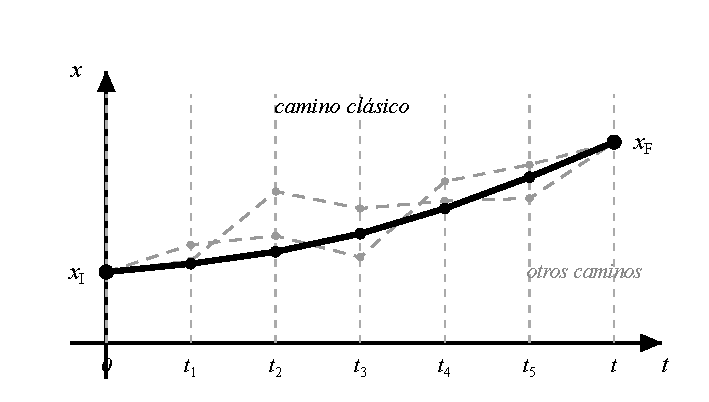
\includegraphics[width=0.66\linewidth]{Capitulo 3/Figuras/IntegralCamino.pdf}
            \caption{Construcción de la integral de camino. El intervalo se divide en rodajas y se integra sobre todas las posiciones intermedias posibles, de manera que a la amplitud contribuyen por igual el camino clásico y todos los caminos quebrados que lo rodean.}
            \label{fig:IntegralCamino}
        \end{figure}

        Sustituyendo \eqref{eq:EslabonFinal} en \eqref{eq:PropagadorRodajas}, el producto de exponenciales se convierte en la exponencial de la suma, y esa suma es una suma de Riemann que en el límite $N\rightarrow\infty$ tiende a la integral de la acción a lo largo del camino poligonal definido por los puntos intermedios,
        \begin{equation}\label{eq:SumaRiemann}
            \sum_{j=0}^{N-1}\varepsilon\left[\frac{m}{2}\left(\frac{x_{j+1}-x_{j}}{\varepsilon}\right)^{2} - V(x_{j})\right]
            \;\xrightarrow[N\rightarrow\infty]{}\;
            \int_{0}^{t}L\left(x,\dot{x}\right)ds = S[x] .
        \end{equation}
        Obtenemos finalmente la \textit{integral de camino de Feynman},
        \begin{equation}\label{eq:IntegralCamino}
            \boxed{\;K(x_{F},t;x_{I},0) = \int_{x(0)=x_{I}}^{x(t)=x_{F}}\mathcal{D}[x(s)]\;\exp\left\{\frac{i}{\hbar}S[x(s)]\right\},\;}
        \end{equation}
        donde el símbolo $\mathcal{D}[x(s)]$ abrevia el límite del producto de integrales sobre los puntos intermedios junto con los factores de normalización,
        \begin{equation}\label{eq:MedidaFeynman}
            \mathcal{D}[x(s)] = \lim_{N\rightarrow\infty}\left(\frac{m}{2\pi i\hbar\varepsilon}\right)^{N/2}\prod_{j=1}^{N-1}dx_{j} .
        \end{equation}

        El significado de \eqref{eq:IntegralCamino} es el que anunciamos al comienzo del capítulo. La amplitud de que la partícula vaya de un punto a otro es la suma de las contribuciones de \textit{todos} los caminos concebibles que los unen, sin excepción, incluidos los que violan groseramente las ecuaciones de movimiento, y cada camino contribuye con el mismo módulo y una fase igual a su acción medida en unidades de $\hbar$. La trayectoria clásica no tiene ningún privilegio a priori; adquiere su privilegio únicamente en el límite en que la acción típica es grande frente a $\hbar$, porque entonces las fases de caminos vecinos oscilan tan rápidamente que sus contribuciones se cancelan entre sí, salvo en la vecindad de aquel camino para el cual la acción es estacionaria y las fases vecinas coinciden en primer orden. \textbf{El principio de Hamilton deja así de ser un postulado y se convierte en el resultado de una interferencia}, y la objeción que se le hizo a Fermat en el siglo XVII, la de que la luz parecía necesitar conocer su destino, queda respondida: la luz no escoge, interfiere.

    \subsection{El propagador del oscilador armónico}

        Aplicaremos ahora el resultado al sistema que nos interesa. Para lagrangianos cuadráticos, como el del oscilador armónico \eqref{eq:LagrangianoOsc}, la integral de camino puede evaluarse exactamente, y el procedimiento consiste en separar cada camino en la trayectoria clásica más una desviación,
        \begin{equation}\label{eq:SeparacionCaminos}
            x(s) = x_{\mathrm{cl}}(s) + y(s), \qquad y(0) = y(t) = 0,
        \end{equation}
        donde la desviación se anula en los extremos porque todos los caminos comparten los mismos puntos inicial y final. Desarrollando la acción en potencias de $y$, y teniendo en cuenta que el término lineal se anula idénticamente porque la acción es estacionaria sobre $x_{\mathrm{cl}}$, que es precisamente lo que afirma el principio de Hamilton, y que para un lagrangiano cuadrático la serie se corta en el segundo orden,
        \begin{equation}\label{eq:AccionSeparada}
            S[x] = S_{\mathrm{cl}} + \textcolor{red}{\left.\frac{\delta S}{\delta x}\right|_{x_{\mathrm{cl}}}\!\!\cdot y} + \frac{1}{2}\left.\frac{\delta^{2}S}{\delta x^{2}}\right|_{x_{\mathrm{cl}}}\!\!\cdot y^{2}
            = S_{\mathrm{cl}} + \int_{0}^{t}\left(\frac{m}{2}\dot{y}^{2} - \frac{m\omega^{2}}{2}y^{2}\right)ds,
        \end{equation}
        donde el término marcado en rojo se anula por la estacionariedad. El factor $e^{iS_{\mathrm{cl}}/\hbar}$ sale entonces fuera de la integral funcional, porque no depende del camino de integración, y lo que queda es una integral sobre desviaciones con extremos nulos que no depende de $x_{I}$ ni de $x_{F}$ sino solo del tiempo transcurrido,
        \begin{equation}\label{eq:PropagadorFactorizado}
            K(x_{F},t;x_{I},0) = F(t)\,\exp\left[\frac{i}{\hbar}S_{\mathrm{cl}}(x_{F},t;x_{I},0)\right] .
        \end{equation}
        La evaluación del prefactor $F(t)$ exige calcular el determinante del operador de fluctuaciones, cálculo que no reproduciremos aquí y cuyo resultado, obtenido por primera vez por Van Vleck en el contexto del principio de correspondencia \citep{vanvleck1928correspondence}, es
        \begin{equation}\label{eq:VanVleck}
            F(t) = \left(\frac{1}{2\pi i\hbar}\,\frac{\partial^{2}S_{\mathrm{cl}}}{\partial x_{I}\,\partial x_{F}}\right)^{1/2} .
        \end{equation}

        Podemos ahora ensamblar el resultado para el oscilador. La acción clásica la calculamos en \eqref{eq:AccionOscilador}, y su derivada cruzada se obtiene derivando esa expresión primero respecto de $q_{I}$ y luego respecto de $q_{F}$: el único término que sobrevive a las dos derivaciones es el producto cruzado, pues los cuadrados desaparecen al derivar respecto de la otra variable,
        \begin{equation}\label{eq:DerivadaCruzada}
            \frac{\partial^{2}S_{\mathrm{cl}}}{\partial q_{I}\,\partial q_{F}}
            = \frac{\partial}{\partial q_{F}}\left[\frac{m\omega}{2\sin\omega t}\left(2q_{I}\cos\omega t - 2q_{F}\right)\right]
            = -\frac{m\omega}{\sin\omega t} .
        \end{equation}
        Sustituyendo \eqref{eq:DerivadaCruzada} en \eqref{eq:VanVleck} y absorbiendo el signo en la determinación de la raíz, el prefactor resulta ser $\left(m\omega/2\pi i\hbar\sin\omega t\right)^{1/2}$, de manera que el propagador completo es
        \begin{equation}\label{eq:PropagadorOscilador}
            \boxed{\;K(q_{F},t;q_{I},0) = \left(\frac{m\omega}{2\pi i\hbar\sin\omega t}\right)^{1/2}
            \exp\left\{\frac{i\,m\omega}{2\hbar}\left[\left(q_{I}^{2}+q_{F}^{2}\right)\cot\omega t - \frac{2q_{I}q_{F}}{\sin\omega t}\right]\right\} .\;}
        \end{equation}

        Esta expresión es el punto de llegada del capítulo y el punto de partida de los dos siguientes. La conexión, dicha explícitamente, es la siguiente. Cuando en el capítulo dedicado a la cuantización del campo electromagnético escribamos el hamiltoniano de cada modo en la forma $H = \frac{1}{2}\left(P^{2}+\omega^{2}Q^{2}\right)$, las variables canónicas estarán normalizadas de manera que la masa efectiva sea la unidad, y entonces \eqref{eq:PropagadorOscilador} se reduce a
        \begin{equation}\label{eq:PropagadorFoton}
            K(q_{F},t;q_{I},0) = \left(\frac{\omega}{2\pi i\hbar\sin\omega t}\right)^{1/2}
            \exp\left\{\frac{i\,\omega}{2\hbar}\left[\left(q_{I}^{2}+q_{F}^{2}\right)\cot\omega t - \frac{2q_{I}q_{F}}{\sin\omega t}\right]\right\},
        \end{equation}
        que es literalmente la amplitud de transición de la que parte el capítulo dedicado a la propagación fundamental de los fotones. \textbf{El propagador del fotón no es, por tanto, un postulado de la óptica cuántica sino la exponencial de la acción clásica de un oscilador armónico, calculada en \eqref{eq:AccionOscilador} sin más herramienta que las ecuaciones de Lagrange.}

        Y hay todavía una observación que merece hacerse, porque cierra el arco completo de estos apuntes. La estructura del exponente de \eqref{eq:PropagadorFoton}, una cotangente multiplicando la suma de los cuadrados y una cosecante multiplicando el producto cruzado, es exactamente la del núcleo de la transformada fraccionaria de Fourier que obtuvimos en el capítulo primero al estudiar la propagación de Fresnel entre dos esferas de referencia, con el ángulo fraccionario $\alpha$ desempeñando el papel de $\omega t$. La difracción de una onda luminosa clásica a lo largo de una distancia $z$ y la evolución temporal de un modo del campo cuantizado durante un tiempo $t$ son, en el plano formal, la misma transformación aplicada a objetos distintos. Esa coincidencia, que a estas alturas ya no puede sorprendernos, es la razón por la cual la óptica y la mecánica cuántica hablan el mismo idioma, y la analogía que Hamilton escribió en 1834 sigue produciendo resultados casi dos siglos después.


	\chapter{Los postulados de la mecánica cuántica}\label{chap:PostuladosQM}
	\thispagestyle{empty}
	\vspace*{2cm}
	\begin{center}
		{\itshape\Huge El estado de un sistema dejó de ser un punto y pasó a ser una dirección en un espacio de infinitas dimensiones. \par}
		\vspace{1cm}
		\epigraph{``No podemos describir los procesos atómicos con el lenguaje de la física clásica, pero tampoco disponemos de otro lenguaje''}{-- Niels Bohr}
	\end{center}
	\clearpage

	\section{Breve historia de la formulación de la mecánica cuántica}

    El capítulo anterior terminó con la ecuación de Schrödinger y con la integral de camino, es decir, con dos maneras distintas de escribir la dinámica cuántica, pero sin haber dicho en ningún momento qué es lo que evoluciona ni qué relación guarda con lo que se mide en un laboratorio. Esa omisión no es un descuido de la exposición sino un reflejo fiel de la historia: la mecánica cuántica se construyó primero como un conjunto de reglas de cálculo que funcionaban, y solo después, y con considerable esfuerzo, se le encontró una estructura matemática coherente y una interpretación. Este capítulo recorre esa estructura y esa interpretación, porque sin ellas el capítulo siguiente, en el cual promoveremos las amplitudes del campo electromagnético a operadores, sería una manipulación formal sin contenido.

    El punto de partida es el verano de 1925 y un joven de veintitrés años enfermo de fiebre del heno. Werner Heisenberg, refugiado en la isla de Helgoland para escapar del polen, decidió abandonar por completo el intento de describir la órbita del electrón y construir una teoría que se refiriese únicamente a cantidades observables, es decir, a las frecuencias y a las intensidades de las líneas espectrales \citep{heisenberg1925umdeutung}. El resultado fue un esquema de cálculo en el que a cada observable le corresponde una tabla doblemente indexada de números, y en el que el producto de dos tablas no conmuta. Heisenberg no sabía que estaba multiplicando matrices; fue Max Born quien lo reconoció al leer el manuscrito, y quien junto con Pascual Jordan escribió la teoría en forma matricial y descubrió la relación fundamental \citep{bornjordan1925zur}
    \begin{equation}\label{eq:ConmutadorHistorico}
        \hat{q}\hat{p} - \hat{p}\hat{q} = i\hbar\,\mathbb{1},
    \end{equation}
    que apareció así, en noviembre de 1925, antes de que existiera ninguna función de onda y sin ninguna interpretación clara de qué era lo que representaba. La versión definitiva del formalismo matricial, extendida a sistemas de varios grados de libertad, se publicó pocos meses después en el célebre trabajo de los tres autores \citep{bornheisenbergjordan1926}.

    En enero de 1926 Schrödinger publicó, como vimos, una teoría completamente distinta en apariencia, basada en una ecuación diferencial para una función de onda continua \citep{schrodinger1926quantisierung}. La coexistencia de dos formalismos que producían los mismos números pero que no se parecían en nada resultaba intolerable, y el propio Schrödinger demostró ese mismo año la equivalencia entre ambos \citep{schrodinger1926verhaltnis}, mostrando que las matrices de Heisenberg son los elementos de matriz de operadores diferenciales entre las funciones propias de su ecuación. La demostración era correcta en el espíritu aunque incompleta en el rigor, y la versión definitiva de la equivalencia, junto con la estructura que hoy llamamos teoría de transformaciones, es obra de Dirac en 1927 \citep{dirac1927physical}.

    Faltaba, sin embargo, lo esencial. Schrödinger creía que $|\psi|^{2}$ describía una densidad de carga real, una especie de nube material extendida, y defendió esa lectura durante años pese a la objeción evidente de que el paquete de ondas de una partícula libre se ensancha indefinidamente mientras que un electrón nunca se observa dividido. La interpretación correcta la propuso Born en junio de 1926, en un artículo sobre colisiones atómicas, y lo hizo en una nota a pie de página añadida durante la corrección de pruebas: $|\psi|^{2}$ no es una densidad de materia sino una \textit{densidad de probabilidad} \citep{born1926stossvorgange}. \textbf{Aquella nota al pie, que Born escribió casi como una enmienda de último momento, es probablemente la frase más consecuente de toda la física del siglo XX}, porque introdujo el azar en el nivel fundamental de la descripción y cambió para siempre el estatus de las leyes físicas. Born recibió el premio Nobel por ella en 1954, veintiocho años después.

    El año siguiente trajo los dos resultados que fijaron el significado físico del formalismo. Heisenberg publicó en 1927 su análisis de lo que puede saberse simultáneamente sobre la posición y el momento de una partícula \citep{heisenberg1927anschaulichen}, obteniendo la relación de indeterminación mediante un argumento sobre el microscopio de rayos gamma que, como veremos, es sugerente pero engañoso; Earle Kennard demostró ese mismo año la versión rigurosa para el caso canónico \citep{kennard1927quantenmechanik} y Howard Robertson la generalizó en 1929 a cualquier par de observables \citep{robertson1929uncertainty}. Y Niels Bohr presentó en el congreso de Como su principio de complementariedad \citep{bohr1928quantum}, según el cual las descripciones ondulatoria y corpuscular no se contradicen sino que se excluyen mutuamente en cada montaje experimental concreto, tesis que sigue siendo el núcleo de la llamada interpretación de Copenhague.

    La arquitectura matemática definitiva llegó en 1932 de la mano de John von Neumann, quien en \textit{Mathematische Grundlagen der Quantenmechanik} demostró que el espacio de funciones de onda de Schrödinger y el espacio de sucesiones de Heisenberg son dos realizaciones del mismo objeto abstracto, un espacio de Hilbert separable, y reformuló toda la teoría en ese lenguaje \citep{vonneumann1932mathematische}. Von Neumann introdujo también, en un trabajo previo de 1927 \citep{vonneumann1927wahrscheinlichkeitstheoretischer} y de manera independiente a Landau, quien llegó al mismo objeto estudiando la emisión espontánea \citep{landau1927dampfungsproblem}, la matriz densidad, que es la herramienta imprescindible cuando el sistema no se encuentra en un estado puro. Esa herramienta, que en su origen era un tecnicismo para tratar subsistemas y mezclas estadísticas, resultó ser el objeto central de la óptica cuántica, porque la luz que emiten las fuentes reales, desde una bombilla hasta una estrella, nunca está en un estado puro.

    El orden de exposición que seguiremos invierte el orden histórico, como es habitual y conveniente. Enunciaremos primero la estructura del espacio de estados, después los postulados en su forma moderna, junto con su interpretación física y con las objeciones que cada uno suscita, y a continuación los resultados que necesitaremos más adelante: el principio de indeterminación, las representaciones de posición y momento, las imágenes de evolución, el oscilador armónico resuelto algebraicamente y, para terminar, la matriz densidad y su conexión con la teoría de la coherencia del capítulo segundo.

\section{El espacio de estados}

        Toda la mecánica cuántica se desarrolla sobre una estructura matemática única, y la definimos con precisión antes de colgar de ella ninguna física.

        \begin{myDef}\label{def:Hilbert}
            Un \textit{espacio de Hilbert} $\mathcal{H}$ es un espacio vectorial sobre el cuerpo de los números complejos, dotado de un producto interno $\langle\cdot\,|\,\cdot\rangle : \mathcal{H}\times\mathcal{H}\rightarrow\mathbb{C}$ que satisface, para todos $\ket{\psi},\ket{\phi},\ket{\chi}\in\mathcal{H}$ y todo $\alpha\in\mathbb{C}$,
            \begin{align}
                \braket{\psi|\phi} &= \overline{\braket{\phi|\psi}} \qquad\text{(simetría hermítica)},\label{eq:SimetriaHermitica}\\
                \braket{\psi|\alpha\phi + \chi} &= \alpha\braket{\psi|\phi} + \braket{\psi|\chi} \qquad\text{(linealidad en el segundo argumento)},\label{eq:LinealidadProducto}\\
                \braket{\psi|\psi} &\geq 0, \quad\text{con igualdad si y solo si}\quad \ket{\psi} = 0 \qquad\text{(definición positiva)},\label{eq:PositividadProducto}
            \end{align}
            y que es \textit{completo} respecto de la norma $\|\psi\| = \sqrt{\braket{\psi|\psi}}$ inducida por ese producto, es decir, toda sucesión de Cauchy de elementos de $\mathcal{H}$ converge a un elemento de $\mathcal{H}$.
        \end{myDef}

        Ninguna de estas condiciones es un capricho del matemático. La estructura de espacio vectorial es la que permite superponer estados, que es el rasgo distintivo de la teoría y el origen de todos los fenómenos de interferencia estudiados en los dos primeros capítulos. El cuerpo tiene que ser el de los complejos y no el de los reales porque, como demostramos en \eqref{eq:SchrodingerTemporal}, la ecuación de evolución es de primer orden en el tiempo con un coeficiente imaginario, de modo que sus soluciones no pueden ser reales. El producto interno proporciona la noción de ángulo entre estados, y será él quien produzca las probabilidades. La condición \eqref{eq:PositividadProducto} garantiza que esas probabilidades sean no negativas. Y la completitud es la que asegura que los procedimientos de límite, como los desarrollos en serie que usaremos constantemente, no nos saquen del espacio.

        Adoptamos desde ahora la notación que Dirac introdujo en 1939 y que es universal en óptica cuántica: los elementos de $\mathcal{H}$ se denotan $\ket{\psi}$ y se llaman \textit{kets}. El producto interno es antilineal en el primer argumento, como se sigue de combinar \eqref{eq:SimetriaHermitica} con \eqref{eq:LinealidadProducto},
        \begin{equation}\label{eq:Antilinealidad}
            \braket{\alpha\psi + \chi|\phi} = \overline{\braket{\phi|\alpha\psi+\chi}} = \overline{\alpha\braket{\phi|\psi} + \braket{\phi|\chi}} = \bar{\alpha}\braket{\psi|\phi} + \braket{\chi|\phi},
        \end{equation}
        y esa asimetría, que al principio incomoda, es la que hace que la norma sea real y positiva pese a que los coeficientes sean complejos.

        A cada ket le corresponde un funcional lineal, el \textit{bra} $\bra{\psi}$, definido por su acción $\bra{\psi}:\ket{\phi}\mapsto\braket{\psi|\phi}$. Que todo funcional lineal continuo sobre $\mathcal{H}$ sea de esta forma, es decir, que la correspondencia entre bras y kets sea biyectiva, es el contenido del teorema de representación de Riesz, y es la razón por la cual la notación de Dirac es consistente: podemos manipular bras y kets como si fuesen objetos del mismo tipo porque el teorema garantiza que hay exactamente uno de cada.

        Un conjunto $\{\ket{n}\}$ de vectores se dice \textit{ortonormal} cuando $\braket{n|m} = \delta_{nm}$, y constituye una \textit{base} cuando además todo estado admite desarrollo,
        \begin{equation}\label{eq:DesarrolloBase}
            \ket{\psi} = \sum_{n} c_{n}\ket{n} .
        \end{equation}
        Los coeficientes se extraen proyectando, es decir, aplicando $\bra{m}$ a ambos lados y usando la ortonormalidad,
        \begin{equation}\label{eq:Coeficientes}
            \braket{m|\psi} = \sum_{n}c_{n}\braket{m|n} = \sum_{n}c_{n}\delta_{mn} = c_{m},
        \end{equation}
        donde la delta ha colapsado la suma dejando un único término. Sustituyendo \eqref{eq:Coeficientes} de nuevo en \eqref{eq:DesarrolloBase},
        \begin{equation}\label{eq:CompletitudPaso}
            \ket{\psi} = \sum_{n}\ket{n}\braket{n|\psi} = \left(\sum_{n}\ket{n}\bra{n}\right)\ket{\psi},
        \end{equation}
        y como esto vale para todo estado, el operador entre paréntesis debe ser la identidad,
        \begin{equation}\label{eq:CompletitudHilbert}
            \boxed{\;\sum_{n}\ket{n}\bra{n} = \hat{\mathbb{1}} .\;}
        \end{equation}
        Esta es la \textit{relación de completitud} o \textit{resolución de la identidad}, y es con diferencia la herramienta de cálculo más utilizada en todo el formalismo: permite insertar una base completa en cualquier punto de una expresión sin alterarla, que es exactamente lo que hicimos al construir la integral de camino en \eqref{eq:Completitud} del capítulo anterior al partir el intervalo temporal en rodajas.

        Los espacios de Hilbert relevantes en física son \textit{separables}, es decir, admiten una base ortonormal numerable, y ese hecho tiene una consecuencia notable: todos ellos son isomorfos entre sí. El espacio $L^{2}(\mathbb{R})$ de las funciones de onda de Schrödinger y el espacio $\ell^{2}$ de las sucesiones de cuadrado sumable de Heisenberg son, como demostró von Neumann, el mismo espacio escrito en dos bases distintas, y esa es la formulación precisa de la equivalencia entre la mecánica ondulatoria y la mecánica matricial. La disputa de 1926 sobre cuál de las dos teorías era la correcta carecía de objeto: eran la misma teoría en dos sistemas de coordenadas.

        Una dificultad técnica surge cuando el observable tiene espectro continuo, como ocurre con la posición de una partícula libre. Los objetos $\ket{x}$ que uno querría usar como base no son normalizables, pues su producto interno es
        \begin{equation}\label{eq:NormalizacionContinua}
            \braket{x|x'} = \delta\left(x-x'\right),
        \end{equation}
        que diverge cuando $x = x'$, de modo que estrictamente no pertenecen al espacio de Hilbert. La relación de completitud adopta entonces la forma integral
        \begin{equation}\label{eq:CompletitudContinua}
            \int_{\mathbb{R}}\ket{x}\bra{x}\,dx = \hat{\mathbb{1}},
        \end{equation}
        y el tratamiento riguroso exige ampliar el espacio de Hilbert a una terna de espacios encajados, la llamada construcción del espacio de Hilbert equipado, en la cual las distribuciones adquieren carta de ciudadanía del mismo modo que en el capítulo primero la hubo de adquirir la delta de Dirac al servir de fuente puntual para la función de Green. No desarrollaremos ese aparato, pero hay que saber que existe y que las manipulaciones formales con $\ket{x}$ están justificadas por él y no por costumbre.

\section{Los postulados}

    Sobre la estructura anterior se levantan cinco enunciados que no se deducen de nada y que constituyen el contenido físico de la teoría. Los presentamos por separado porque cada uno responde a una pregunta distinta, a saber, qué describe el estado de un sistema, qué representa una magnitud medible, qué ocurre al medirla, cómo evoluciona el sistema cuando no se le mide y cómo se combinan dos sistemas en uno solo. Tras cada enunciado discutiremos su contenido y, cuando lo haya, también sus dificultades.

    \subsection{Primer postulado: el estado}

        \begin{Assumption}[Estado]\label{sup:Estado}
            El estado de un sistema físico aislado en un instante dado queda completamente descrito por un vector $\ket{\psi}$ de norma unidad perteneciente a un espacio de Hilbert $\mathcal{H}$ asociado al sistema. Dos vectores que difieran en un factor de fase global, $\ket{\psi}$ y $e^{i\theta}\ket{\psi}$, describen el mismo estado físico.
        \end{Assumption}

        Tres afirmaciones distintas se esconden en este enunciado, y las separamos porque su contenido físico es muy diferente.

        La primera es que la descripción es \textit{completa}. El vector de estado no es un resumen estadístico de nuestra ignorancia sobre variables ocultas más finas, al modo en que la distribución de velocidades de un gas resume nuestra ignorancia sobre las trayectorias individuales; es todo lo que hay que saber. Esta afirmación fue rechazada por Einstein, quien en el artículo de 1935 escrito con Podolsky y Rosen argumentó que la descripción cuántica debía ser incompleta, y el debate permaneció abierto hasta que Bell formuló en 1964 una desigualdad que permitía someterlo a prueba experimental. Los experimentos de Aspect y colaboradores, que este libro discute en el capítulo siguiente, dieron la razón a la mecánica cuántica.

        La segunda es el \textit{principio de superposición}. Si $\ket{\psi_{1}}$ y $\ket{\psi_{2}}$ son estados posibles, también lo es cualquier combinación lineal normalizada
        \begin{equation}\label{eq:Superposicion}
            \ket{\psi} = c_{1}\ket{\psi_{1}} + c_{2}\ket{\psi_{2}},
            \qquad
            |c_{1}|^{2} + |c_{2}|^{2} = 1 \quad\text{si}\quad \braket{\psi_{1}|\psi_{2}} = 0 .
        \end{equation}
        Este principio es el responsable directo de todos los fenómenos de interferencia, y merece subrayarse que es el mismo principio que gobierna las ondas clásicas estudiadas en los capítulos primero y segundo. La diferencia entre la interferencia clásica y la cuántica no está en la superposición, que es idéntica, sino en qué es lo que se superpone: allí se superponen campos cuyo cuadrado es una intensidad medible, aquí se superponen amplitudes cuyo cuadrado es una probabilidad.

        La tercera es la irrelevancia de la \textit{fase global}. Que $\ket{\psi}$ y $e^{i\theta}\ket{\psi}$ sean físicamente indistinguibles significa que el estado no es propiamente un vector sino un rayo, es decir, una clase de equivalencia de vectores que difieren en un factor complejo de módulo unidad. Hay que ser muy cuidadoso aquí, porque el estudiante confunde con facilidad este enunciado con la afirmación, radicalmente falsa, de que las fases no importan. Consideremos la superposición
        \begin{equation}\label{eq:FaseRelativa}
            \ket{\psi_{\theta}} = \frac{1}{\sqrt{2}}\left(\ket{\psi_{1}} + e^{i\theta}\ket{\psi_{2}}\right),
        \end{equation}
        cuya fase $\theta$ es \textit{relativa} entre las dos componentes y no global. Si multiplicamos el estado completo por $e^{i\varphi}$ nada cambia, pero si variamos $\theta$ el estado cambia por completo, y de hecho \eqref{eq:FaseRelativa} recorre un conjunto continuo de estados físicamente distintos a medida que $\theta$ varía entre $0$ y $2\pi$. \textbf{Las fases relativas son observables y las globales no lo son}, y toda la interferometría, clásica y cuántica, consiste en convertir fases relativas en diferencias de intensidad medibles.

    \subsection{Segundo postulado: los observables}

        \begin{Assumption}[Observables]\label{sup:Observables}
            A toda magnitud física medible $A$ le corresponde un operador lineal autoadjunto $\hat{A}$ que actúa sobre el espacio de Hilbert del sistema. Los únicos resultados posibles de una medida de $A$ son los elementos del espectro de $\hat{A}$.
        \end{Assumption}

        La exigencia de linealidad es consistente con el principio de superposición, pues un operador no lineal destruiría la estructura del espacio. La exigencia de autoadjunción, es decir, de que $\hat{A}^{\dagger} = \hat{A}$ con igualdad también de los dominios de definición, tiene una motivación física inmediata que pasamos a demostrar.

        \begin{myteo}\label{teo:ValoresPropiosReales}
            Los valores propios de un operador autoadjunto son reales, y los vectores propios correspondientes a valores propios distintos son ortogonales.
        \end{myteo}

        \textbf{\textit{Demostración:}} sea $\hat{A}\ket{a} = a\ket{a}$ con $\ket{a}\neq 0$. Tomando el producto interno con el propio $\ket{a}$ obtenemos
        \begin{equation}\label{eq:ValorPropioReal1}
            \braket{a|\hat{A}|a} = a\braket{a|a},
        \end{equation}
        y tomando el complejo conjugado de esta igualdad, y usando la simetría hermítica \eqref{eq:SimetriaHermitica} junto con la definición de adjunto y la hipótesis $\hat{A}^{\dagger} = \hat{A}$,
        \begin{equation}\label{eq:ValorPropioReal2}
            \overline{\braket{a|\hat{A}|a}} = \braket{a|\hat{A}^{\dagger}|a} = \braket{a|\hat{A}|a} = \bar{a}\braket{a|a} .
        \end{equation}
        Restando \eqref{eq:ValorPropioReal2} de \eqref{eq:ValorPropioReal1} resulta $\left(a - \bar{a}\right)\braket{a|a} = 0$, y como la norma es estrictamente positiva por \eqref{eq:PositividadProducto}, concluimos $a = \bar{a}$, es decir, $a$ es real.

        Para la segunda afirmación, sean $\hat{A}\ket{a} = a\ket{a}$ y $\hat{A}\ket{b} = b\ket{b}$ con $a\neq b$. Podemos calcular $\braket{b|\hat{A}|a}$ de dos maneras: dejando actuar el operador hacia la derecha se obtiene $a\braket{b|a}$, y dejándolo actuar hacia la izquierda, lo que es lícito por ser autoadjunto, se obtiene $\bar{b}\braket{b|a} = b\braket{b|a}$ puesto que $b$ ya sabemos que es real. Igualando ambos resultados,
        \begin{equation}\label{eq:Ortogonalidad}
            \left(a - b\right)\braket{b|a} = 0,
        \end{equation}
        y como $a\neq b$ por hipótesis, necesariamente $\braket{b|a} = 0$. $\blacksquare$

        El teorema explica exactamente por qué los observables deben ser autoadjuntos: los resultados de las medidas son números reales, de modo que los valores propios han de serlo. La ortogonalidad, por su parte, tiene una lectura física igualmente directa: dos estados con valores distintos de una misma magnitud son perfectamente distinguibles, pues una medida los separa sin ambigüedad, y la ortogonalidad es la traducción geométrica de esa distinguibilidad.

        El teorema espectral, que no demostraremos, garantiza además que los vectores propios de un operador autoadjunto forman una base completa del espacio, de modo que todo observable lleva asociada una descomposición
        \begin{equation}\label{eq:DescomposicionEspectral}
            \hat{A} = \sum_{n} a_{n}\ket{a_{n}}\bra{a_{n}} = \sum_{n} a_{n}\hat{P}_{n},
            \qquad
            \hat{P}_{n} \equiv \ket{a_{n}}\bra{a_{n}},
        \end{equation}
        donde los $\hat{P}_{n}$ son proyectores ortogonales que satisfacen $\hat{P}_{n}\hat{P}_{m} = \delta_{nm}\hat{P}_{n}$ y $\sum_{n}\hat{P}_{n} = \hat{\mathbb{1}}$. Nótese que \eqref{eq:DescomposicionEspectral} contiene toda la información sobre el observable: los valores que puede arrojar una medida y las direcciones del espacio asociadas a cada uno de ellos.

        Merece una advertencia la distinción entre hermítico y autoadjunto, que en dimensión finita es vacua pero en dimensión infinita no lo es. Un operador puede satisfacer $\braket{\phi|\hat{A}\psi} = \braket{\hat{A}\phi|\psi}$ para todo par de vectores de su dominio y no ser autoadjunto, si el dominio de su adjunto es estrictamente mayor. El ejemplo clásico es el operador de momento en un intervalo finito, que admite una familia de extensiones autoadjuntas distintas según la condición de contorno que se imponga, y cada extensión describe una física diferente. Esta sutileza reaparecerá en el capítulo siguiente al intentar definir un operador de fase para el campo electromagnético, problema que Dirac abordó ingenuamente en 1927 y que resultó ser mucho más delicado de lo que parecía.

    \subsection{Tercer postulado: la medida}

        \begin{Assumption}[Regla de Born]\label{sup:Born}
            Si el sistema se encuentra en el estado normalizado $\ket{\psi}$ y se mide el observable $\hat{A}$, la probabilidad de obtener el valor propio $a_{n}$ es
            \begin{equation}\label{eq:ReglaBorn}
                P(a_{n}) = \left|\braket{a_{n}|\psi}\right|^{2} = \braket{\psi|\hat{P}_{n}|\psi},
            \end{equation}
            e inmediatamente después de la medida el sistema queda en el estado propio correspondiente,
            \begin{equation}\label{eq:Colapso}
                \ket{\psi} \;\longrightarrow\; \frac{\hat{P}_{n}\ket{\psi}}{\sqrt{\braket{\psi|\hat{P}_{n}|\psi}}} .
            \end{equation}
        \end{Assumption}

        \begin{figure}[htbp]
            \centering
            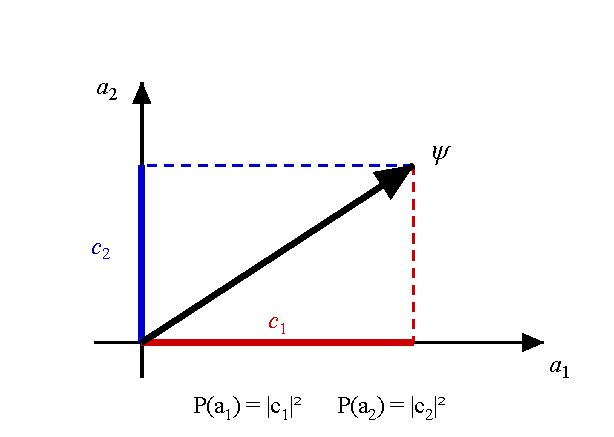
\includegraphics[width=0.56\linewidth]{Capitulo 4/Figuras/MedidaProyeccion.pdf}
            \caption{Contenido geométrico de la regla de Born. El estado se descompone en la base propia del observable y la probabilidad de cada resultado es el cuadrado del módulo de la componente correspondiente.}
            \label{fig:MedidaProyeccion}
        \end{figure}

        La prescripción es consistente, es decir, las probabilidades suman uno. Sumando \eqref{eq:ReglaBorn} sobre todos los resultados posibles y usando la completitud de la base de vectores propios,
        \begin{equation}\label{eq:SumaProbabilidades}
            \sum_{n}P(a_{n}) = \sum_{n}\braket{\psi|\hat{P}_{n}|\psi} = \braket{\psi|\left(\sum_{n}\hat{P}_{n}\right)|\psi} = \braket{\psi|\hat{\mathbb{1}}|\psi} = \braket{\psi|\psi} = 1,
        \end{equation}
        donde el último paso usa la normalización exigida en el postulado \ref{sup:Estado}. La normalización del estado y la conservación de la probabilidad son, por tanto, la misma condición, y esa es la razón de que el primer postulado exija norma unidad.

        De la regla de Born se sigue de inmediato la expresión del valor medio de una magnitud, que es la cantidad que efectivamente se compara con el experimento cuando la medida se repite muchas veces sobre sistemas preparados de manera idéntica. Por definición de promedio estadístico,
        \begin{equation}\label{eq:ValorMedio1}
            \left\langle A\right\rangle = \sum_{n} a_{n}P(a_{n}) = \sum_{n}a_{n}\braket{\psi|\hat{P}_{n}|\psi} = \braket{\psi|\left(\sum_{n}a_{n}\hat{P}_{n}\right)|\psi},
        \end{equation}
        y reconociendo en el paréntesis la descomposición espectral \eqref{eq:DescomposicionEspectral} del propio operador obtenemos la fórmula fundamental
        \begin{equation}\label{eq:ValorMedio}
            \boxed{\;\left\langle A\right\rangle_{\psi} = \braket{\psi|\hat{A}|\psi} .\;}
        \end{equation}
        Este resultado no es un postulado adicional sino una consecuencia de \eqref{eq:ReglaBorn}, y hay que tenerlo presente porque en muchos textos se enuncia como si fuese independiente.

        La segunda parte del postulado, la proyección del estado tras la medida, es con mucho la más problemática de toda la teoría y sería deshonesto presentarla sin señalarlo. Su justificación operativa es sólida: si medimos dos veces seguidas la misma magnitud sin dar tiempo al sistema a evolucionar, obtenemos el mismo resultado, y la única manera de que la teoría reproduzca ese hecho experimental es que la primera medida haya dejado al sistema en el estado propio correspondiente. En efecto, aplicando \eqref{eq:ReglaBorn} al estado proyectado,
        \begin{equation}\label{eq:MedidaRepetida}
            P'(a_{m}) = \frac{\braket{\psi|\hat{P}_{n}\hat{P}_{m}\hat{P}_{n}|\psi}}{\braket{\psi|\hat{P}_{n}|\psi}} = \frac{\delta_{nm}\braket{\psi|\hat{P}_{n}|\psi}}{\braket{\psi|\hat{P}_{n}|\psi}} = \delta_{nm},
        \end{equation}
        donde hemos usado la ortogonalidad de los proyectores, de manera que el segundo resultado coincide con el primero con certeza.

        La dificultad es de otro orden y es la siguiente. El cuarto postulado, que enunciaremos a continuación, afirma que la evolución de un sistema aislado es unitaria, y por tanto lineal, determinista y reversible; el tercero afirma que la medida produce un salto no lineal, indeterminista e irreversible. Un aparato de medida está hecho de átomos y debería obedecer al cuarto postulado, de modo que la teoría contiene dos leyes de evolución incompatibles y no especifica dónde está la frontera entre sus dominios de aplicación. Esta es la formulación precisa del llamado \textit{problema de la medida}, y no está resuelto. Las respuestas que se han propuesto van desde negar que el colapso sea un proceso físico, como en la interpretación de Copenhague, hasta negar que ocurra en absoluto, como en la interpretación de los muchos mundos, pasando por modificar la ecuación de evolución para que el colapso emerja de ella, como en los modelos de colapso espontáneo. La teoría de la decoherencia explica de manera satisfactoria por qué las superposiciones macroscópicas se vuelven inobservables con enorme rapidez, y ese es un avance genuino, pero no explica por qué de todos los resultados posibles se realiza uno concreto. Que una teoría con esta fisura conceptual sea al mismo tiempo la más precisa jamás construida, con predicciones verificadas hasta la duodécima cifra decimal, es probablemente el hecho más desconcertante de la física contemporánea.

        Cuando el valor propio $a_{n}$ está degenerado, es decir, cuando le corresponde un subespacio de dimensión mayor que uno, la regla de proyección debe formularse con el proyector sobre todo el subespacio y no sobre un vector particular, como estableció Lüders en 1950 \citep{luders1950zustandsanderung}; las expresiones \eqref{eq:ReglaBorn} y \eqref{eq:Colapso} ya están escritas en esa forma general, y por eso hemos preferido escribirlas con proyectores en lugar de con productos escalares.

    \subsection{Cuarto postulado: la evolución}

        \begin{Assumption}[Evolución]\label{sup:Evolucion}
            Entre medidas, el estado de un sistema aislado evoluciona de manera determinista según la ecuación de Schrödinger
            \begin{equation}\label{eq:SchrodingerPostulado}
                i\hbar\frac{d}{dt}\ket{\psi(t)} = \hat{H}\ket{\psi(t)},
            \end{equation}
            donde $\hat{H}$ es el operador hamiltoniano del sistema, obtenido del hamiltoniano clásico mediante la correspondencia canónica.
        \end{Assumption}

        La estructura de esta evolución se entiende mejor introduciendo el \textit{operador de evolución} $\hat{U}(t,t_{0})$ definido por
        \begin{equation}\label{eq:OperadorEvolucion}
            \ket{\psi(t)} = \hat{U}(t,t_{0})\ket{\psi(t_{0})},
        \end{equation}
        que para un hamiltoniano independiente del tiempo se obtiene integrando formalmente \eqref{eq:SchrodingerPostulado},
        \begin{equation}\label{eq:ExponencialEvolucion}
            \hat{U}(t,t_{0}) = \exp\left[-\frac{i}{\hbar}\hat{H}\left(t-t_{0}\right)\right],
        \end{equation}
        donde la exponencial de un operador se define mediante su serie de potencias. Que esta expresión resuelve la ecuación se comprueba derivándola término a término,
        \begin{equation}\label{eq:VerificacionU}
            i\hbar\frac{d\hat{U}}{dt} = i\hbar\left(-\frac{i}{\hbar}\hat{H}\right)\exp\left[-\frac{i}{\hbar}\hat{H}(t-t_{0})\right] = \hat{H}\hat{U},
        \end{equation}
        donde el producto $i\hbar\cdot(-i/\hbar) = 1$ deja exactamente el hamiltoniano.

        La propiedad esencial de esta evolución es su unitariedad, que demostramos a continuación porque es el fundamento de la conservación de la probabilidad.

        \begin{myteo}\label{teo:Unitariedad}
            Si $\hat{H}$ es autoadjunto, entonces el operador de evolución satisface $\hat{U}^{\dagger}\hat{U} = \hat{U}\hat{U}^{\dagger} = \hat{\mathbb{1}}$, y en consecuencia la norma del estado se conserva.
        \end{myteo}

        \textbf{\textit{Demostración:}} el adjunto de la exponencial se obtiene conjugando la serie término a término, lo que cambia el signo del exponente imaginario y sustituye $\hat{H}$ por $\hat{H}^{\dagger}$,
        \begin{equation}\label{eq:AdjuntoU}
            \hat{U}^{\dagger} = \exp\left[+\frac{i}{\hbar}\hat{H}^{\dagger}\left(t-t_{0}\right)\right] = \exp\left[+\frac{i}{\hbar}\hat{H}\left(t-t_{0}\right)\right],
        \end{equation}
        donde el segundo paso usa la hipótesis $\hat{H}^{\dagger} = \hat{H}$. Multiplicando ambos operadores, y teniendo en cuenta que las exponenciales de un mismo operador conmutan entre sí, de manera que sus exponentes se suman,
        \begin{equation}\label{eq:ProductoU}
            \hat{U}^{\dagger}\hat{U} = \exp\left[\textcolor{red}{+\frac{i}{\hbar}\hat{H}(t-t_{0})} \textcolor{red}{-\frac{i}{\hbar}\hat{H}(t-t_{0})}\right] = \exp\left(0\right) = \hat{\mathbb{1}},
        \end{equation}
        donde los dos exponentes marcados en rojo se cancelan idénticamente. La conservación de la norma se sigue de inmediato,
        \begin{equation}\label{eq:ConservacionNorma}
            \braket{\psi(t)|\psi(t)} = \braket{\psi(t_{0})|\hat{U}^{\dagger}\hat{U}|\psi(t_{0})} = \braket{\psi(t_{0})|\psi(t_{0})} = 1 . \qquad\blacksquare
        \end{equation}

        La lectura física de este teorema es que la autoadjunción del hamiltoniano, que ya habíamos exigido por ser la energía un observable, garantiza además que la probabilidad total no se pierda durante la evolución. Un hamiltoniano no autoadjunto describiría un sistema en el cual las partículas desaparecen, y de hecho los hamiltonianos efectivos no hermíticos se usan deliberadamente en óptica para describir medios con pérdidas, donde los fotones son absorbidos y la probabilidad de detectarlos efectivamente disminuye.

        Hay además una relación entre este postulado y el capítulo anterior. Comparando \eqref{eq:ExponencialEvolucion} con el propagador \eqref{eq:DefinicionPropagador} que definimos allí vemos que el núcleo de Feynman no es otra cosa que el elemento de matriz del operador de evolución entre estados de posición,
        \begin{equation}\label{eq:PropagadorComoU}
            K(x_{F},t;x_{I},0) = \braket{x_{F}|\hat{U}(t,0)|x_{I}},
        \end{equation}
        de modo que la integral de camino \eqref{eq:IntegralCamino} es una manera de calcular la exponencial de un operador sumando sobre trayectorias clásicas. Los dos formalismos son equivalentes y usaremos uno u otro según convenga.

    \subsection{Quinto postulado: sistemas compuestos}

        \begin{Assumption}[Composición]\label{sup:Composicion}
            El espacio de estados de un sistema compuesto por dos subsistemas $A$ y $B$ es el producto tensorial de los espacios de cada uno,
            \begin{equation}\label{eq:ProductoTensorial}
                \mathcal{H}_{AB} = \mathcal{H}_{A}\otimes\mathcal{H}_{B} .
            \end{equation}
        \end{Assumption}

        Si $\{\ket{a_{i}}\}$ y $\{\ket{b_{j}}\}$ son bases de cada factor, entonces $\{\ket{a_{i}}\otimes\ket{b_{j}}\}$ es una base del conjunto, de manera que la dimensión del espacio compuesto es el \textit{producto} de las dimensiones y no su suma, como ocurriría en una suma directa. Esa diferencia, que parece puramente aritmética, tiene una consecuencia física enorme: el estado más general del sistema compuesto,
        \begin{equation}\label{eq:EstadoCompuesto}
            \ket{\Psi} = \sum_{i,j}c_{ij}\,\ket{a_{i}}\otimes\ket{b_{j}},
        \end{equation}
        no puede en general factorizarse en la forma $\ket{\psi_{A}}\otimes\ket{\psi_{B}}$, pues para que ello ocurra la matriz de coeficientes $c_{ij}$ debe tener rango uno, condición que la inmensa mayoría de las matrices no cumple. Los estados que no admiten esa factorización se llaman \textit{entrelazados}, y son la regla y no la excepción.

        Merece la pena detenerse en lo que acaba de aparecer, porque no es un tecnicismo del producto tensorial. La existencia de estados entrelazados es la consecuencia más profunda del formalismo y la que separa de manera más nítida a la física cuántica de la clásica, porque en un estado entrelazado el sistema compuesto está en un estado puro, es decir, perfectamente determinado, mientras que ninguno de sus subsistemas lo está. El todo está mejor definido que las partes, afirmación que no tiene ningún análogo clásico posible. Para describir el estado de uno solo de los subsistemas necesitaremos la matriz densidad, que introduciremos al final del capítulo, y que es precisamente el objeto que la teoría exige cuando se renuncia a mirar el sistema completo.

\section{Compatibilidad y el principio de indeterminación}

        El hecho de que los observables sean operadores, y de que los operadores en general no conmuten, introduce en la física una restricción que no tiene contrapartida clásica: no todas las magnitudes pueden determinarse simultáneamente. El resultado preciso es el siguiente.

        \begin{myteo}\label{teo:Compatibles}
            Dos observables $\hat{A}$ y $\hat{B}$ admiten un conjunto completo de vectores propios comunes si y solo si conmutan, $[\hat{A},\hat{B}] = 0$.
        \end{myteo}

        \textbf{\textit{Demostración:}} supongamos primero que existe una base común $\{\ket{n}\}$ tal que $\hat{A}\ket{n} = a_{n}\ket{n}$ y $\hat{B}\ket{n} = b_{n}\ket{n}$. Aplicando el conmutador a cualquier elemento de la base,
        \begin{equation}\label{eq:ConmutadorBase}
            \left[\hat{A},\hat{B}\right]\ket{n} = \hat{A}\hat{B}\ket{n} - \hat{B}\hat{A}\ket{n} = b_{n}\hat{A}\ket{n} - a_{n}\hat{B}\ket{n} = \left(\textcolor{red}{a_{n}b_{n}} - \textcolor{red}{b_{n}a_{n}}\right)\ket{n} = 0,
        \end{equation}
        donde los dos productos marcados en rojo se cancelan por ser números y conmutar entre sí. Como el conmutador anula a todos los elementos de una base, y es lineal, anula a todo el espacio y por tanto es el operador nulo.

        Recíprocamente, supongamos $[\hat{A},\hat{B}] = 0$ y sea $\ket{a}$ un vector propio de $\hat{A}$ con valor propio $a$ no degenerado. Entonces
        \begin{equation}\label{eq:ReciprocoConmutan}
            \hat{A}\left(\hat{B}\ket{a}\right) = \hat{B}\hat{A}\ket{a} = a\left(\hat{B}\ket{a}\right),
        \end{equation}
        donde el primer paso usa la conmutación. La igualdad afirma que el vector $\hat{B}\ket{a}$ es también vector propio de $\hat{A}$ con el mismo valor propio $a$, y como hemos supuesto que ese valor propio no está degenerado, el subespacio correspondiente tiene dimensión uno y por tanto $\hat{B}\ket{a}$ debe ser proporcional a $\ket{a}$,
        \begin{equation}\label{eq:BEsPropio}
            \hat{B}\ket{a} = b\ket{a},
        \end{equation}
        es decir, $\ket{a}$ es también vector propio de $\hat{B}$. Cuando hay degeneración el argumento se aplica dentro de cada subespacio propio de $\hat{A}$, donde $\hat{B}$ actúa como un operador autoadjunto y puede diagonalizarse por el teorema espectral. $\blacksquare$

        La interpretación física es directa, pero hay que enunciarla con cuidado, porque se presta a confusión. Si dos observables conmutan, existe una base de estados en los cuales ambos tienen valor definido, y medir uno no perturba el valor del otro, de modo que pueden medirse en cualquier orden con resultados reproducibles; se dice entonces que son \textit{compatibles}. Si no conmutan, no existe tal base, y la afirmación de que el sistema posee simultáneamente valores definidos de ambas magnitudes carece de sentido dentro de la teoría. No se trata de que el sistema tenga esos valores y nosotros no podamos conocerlos, sino de que la teoría no le atribuye tales valores, y esta distinción, que Bohr insistió en subrayar durante toda su vida, es la diferencia entre la mecánica cuántica y una teoría clásica con ignorancia añadida.

        Un conjunto de observables que conmutan dos a dos y cuyos valores propios simultáneos identifican unívocamente a cada elemento de la base se llama \textit{conjunto completo de observables compatibles}, y proporciona la manera sistemática de etiquetar los estados de un sistema. En el capítulo siguiente los estados del campo electromagnético en una cavidad se etiquetarán mediante los números de ocupación de todos los modos, que forman precisamente un conjunto de esta clase.

        La incompatibilidad admite una formulación cuantitativa. Definamos la \textit{dispersión} de un observable en un estado dado como la raíz cuadrada de la varianza,
        \begin{equation}\label{eq:Dispersion}
            \left(\Delta A\right)^{2} \equiv \left\langle\left(\hat{A} - \left\langle A\right\rangle\right)^{2}\right\rangle = \left\langle \hat{A}^{2}\right\rangle - \left\langle A\right\rangle^{2},
        \end{equation}
        donde la segunda igualdad se obtiene desarrollando el cuadrado y usando la linealidad del valor medio. La dispersión mide cuánto fluctúan los resultados de la medida alrededor de su promedio, y se anula si y solo si el estado es un vector propio del observable.

        \begin{myteo}[Robertson]\label{teo:Robertson}
            Para cualesquiera dos observables $\hat{A}$ y $\hat{B}$ y cualquier estado normalizado $\ket{\psi}$ se cumple
            \begin{equation}\label{eq:Robertson}
                \Delta A\,\Delta B \;\geq\; \frac{1}{2}\left|\left\langle\left[\hat{A},\hat{B}\right]\right\rangle\right| .
            \end{equation}
        \end{myteo}

        \textbf{\textit{Demostración:}} definamos los operadores centrados
        \begin{equation}\label{eq:OperadoresCentrados}
            \hat{\mathcal{A}} = \hat{A} - \left\langle A\right\rangle, \qquad \hat{\mathcal{B}} = \hat{B} - \left\langle B\right\rangle,
        \end{equation}
        que son autoadjuntos por serlo $\hat{A}$ y $\hat{B}$ y por ser reales sus valores medios, y que satisfacen $\left(\Delta A\right)^{2} = \braket{\psi|\hat{\mathcal{A}}^{2}|\psi}$ y análogamente para $\hat{\mathcal{B}}$. Su conmutador, además, coincide con el de los operadores originales, pues las constantes conmutan con todo,
        \begin{equation}\label{eq:ConmutadorCentrado}
            \left[\hat{\mathcal{A}},\hat{\mathcal{B}}\right] = \left[\hat{A} - \left\langle A\right\rangle,\;\hat{B} - \left\langle B\right\rangle\right] = \left[\hat{A},\hat{B}\right] .
        \end{equation}

        Con los vectores $\ket{u} = \hat{\mathcal{A}}\ket{\psi}$ y $\ket{v} = \hat{\mathcal{B}}\ket{\psi}$, cuyas normas al cuadrado son precisamente las varianzas, se tiene
        \begin{equation}\label{eq:NormasUV}
            \braket{u|u} = \braket{\psi|\hat{\mathcal{A}}^{\dagger}\hat{\mathcal{A}}|\psi} = \braket{\psi|\hat{\mathcal{A}}^{2}|\psi} = \left(\Delta A\right)^{2},
            \qquad
            \braket{v|v} = \left(\Delta B\right)^{2} .
        \end{equation}
        La desigualdad de Cauchy y Schwarz, válida en todo espacio con producto interno, afirma que
        \begin{equation}\label{eq:CauchySchwarz}
            \braket{u|u}\braket{v|v} \geq \left|\braket{u|v}\right|^{2},
        \end{equation}
        de manera que el problema se reduce a acotar inferiormente el miembro derecho. El número complejo $\braket{u|v}$ se separa en sus partes real e imaginaria como
        \begin{equation}\label{eq:SeparacionZ}
            \braket{u|v} = \braket{\psi|\hat{\mathcal{A}}\hat{\mathcal{B}}|\psi} = \frac{1}{2}\braket{\psi|\left\{\hat{\mathcal{A}},\hat{\mathcal{B}}\right\}|\psi} + \frac{1}{2}\braket{\psi|\left[\hat{\mathcal{A}},\hat{\mathcal{B}}\right]|\psi},
        \end{equation}
        donde hemos usado la identidad $\hat{\mathcal{A}}\hat{\mathcal{B}} = \frac{1}{2}\{\hat{\mathcal{A}},\hat{\mathcal{B}}\} + \frac{1}{2}[\hat{\mathcal{A}},\hat{\mathcal{B}}]$, que se comprueba desarrollando el anticonmutador y el conmutador y observando que los términos $\hat{\mathcal{B}}\hat{\mathcal{A}}$ se cancelan,
        \begin{equation}\label{eq:IdentidadAntiConm}
            \frac{1}{2}\left(\hat{\mathcal{A}}\hat{\mathcal{B}} + \textcolor{red}{\hat{\mathcal{B}}\hat{\mathcal{A}}}\right) + \frac{1}{2}\left(\hat{\mathcal{A}}\hat{\mathcal{B}} - \textcolor{red}{\hat{\mathcal{B}}\hat{\mathcal{A}}}\right) = \hat{\mathcal{A}}\hat{\mathcal{B}} .
        \end{equation}

        Los dos términos de \eqref{eq:SeparacionZ} tienen carácter distinto, y esa es la clave de la demostración. El anticonmutador de dos operadores autoadjuntos es autoadjunto, de modo que su valor medio es real; el conmutador de dos operadores autoadjuntos es antiautoadjunto, pues
        \begin{equation}\label{eq:ConmutadorAntihermitico}
            \left[\hat{\mathcal{A}},\hat{\mathcal{B}}\right]^{\dagger} = \left(\hat{\mathcal{A}}\hat{\mathcal{B}}\right)^{\dagger} - \left(\hat{\mathcal{B}}\hat{\mathcal{A}}\right)^{\dagger} = \hat{\mathcal{B}}\hat{\mathcal{A}} - \hat{\mathcal{A}}\hat{\mathcal{B}} = -\left[\hat{\mathcal{A}},\hat{\mathcal{B}}\right],
        \end{equation}
        y el valor medio de un operador antiautoadjunto es imaginario puro. El módulo al cuadrado de \eqref{eq:SeparacionZ} es por tanto la suma de los cuadrados de ambas contribuciones,
        \begin{equation}\label{eq:ModuloZ}
            \left|\braket{u|v}\right|^{2} = \frac{1}{4}\left|\left\langle\left\{\hat{\mathcal{A}},\hat{\mathcal{B}}\right\}\right\rangle\right|^{2} + \frac{1}{4}\left|\left\langle\left[\hat{\mathcal{A}},\hat{\mathcal{B}}\right]\right\rangle\right|^{2}
            \;\geq\; \frac{1}{4}\left|\left\langle\left[\hat{\mathcal{A}},\hat{\mathcal{B}}\right]\right\rangle\right|^{2},
        \end{equation}
        donde la desigualdad final se obtiene simplemente descartando el primer sumando, que es no negativo. Combinando \eqref{eq:NormasUV}, \eqref{eq:CauchySchwarz} y \eqref{eq:ModuloZ}, y usando \eqref{eq:ConmutadorCentrado},
        \begin{equation}\label{eq:RobertsonFinal}
            \left(\Delta A\right)^{2}\left(\Delta B\right)^{2} \geq \frac{1}{4}\left|\left\langle\left[\hat{A},\hat{B}\right]\right\rangle\right|^{2},
        \end{equation}
        y tomando la raíz cuadrada, que preserva la desigualdad por ser ambos miembros no negativos, se obtiene \eqref{eq:Robertson}. $\blacksquare$

        Aplicando el teorema al par canónico, cuyo conmutador es el número $i\hbar$ según \eqref{eq:ConmutadorHistorico}, el valor medio se calcula de inmediato porque una constante sale fuera y el estado está normalizado,
        \begin{equation}\label{eq:HeisenbergCanonico}
            \Delta x\,\Delta p \geq \frac{1}{2}\left|\braket{\psi|i\hbar|\psi}\right| = \frac{\hbar}{2}\left|\braket{\psi|\psi}\right| = \frac{\hbar}{2},
        \end{equation}
        que es la relación de indeterminación de Heisenberg en la forma precisa que le dio Kennard \citep{kennard1927quantenmechanik}.

        La interpretación de \eqref{eq:HeisenbergCanonico} exige cuidado porque la que popularizó Heisenberg es incorrecta, o al menos gravemente incompleta. El argumento del microscopio de rayos gamma, según el cual al iluminar el electrón con un fotón de longitud de onda corta se le transfiere un momento incontrolado, describe un efecto real pero sugiere que la partícula \textit{tiene} una posición y un momento definidos que la medida perturba. Nada en la demostración anterior se refiere a perturbación alguna: la desigualdad \eqref{eq:Robertson} es una propiedad del estado, no del procedimiento de medida, y afirma que \textbf{no existe ningún estado en el cual ambas dispersiones sean simultáneamente arbitrariamente pequeñas}. Las dispersiones se determinan midiendo cada magnitud sobre sistemas distintos preparados de manera idéntica, de modo que ni siquiera hace falta medir ambas sobre el mismo sistema para que la relación se manifieste. La indeterminación es una propiedad de la preparación y no del acto de medir.

        Vale la pena añadir, porque lo usaremos en el capítulo siguiente, que la desigualdad \eqref{eq:HeisenbergCanonico} se satura, es decir, se convierte en igualdad, precisamente para los estados gaussianos, y que en el contexto del campo electromagnético esa saturación define a los estados coherentes y, cuando además se redistribuye la incertidumbre entre las dos cuadraturas, a los estados comprimidos. La luz comprimida consiste en explotar el hecho de que \eqref{eq:HeisenbergCanonico} acota el producto de las dispersiones y no cada una de ellas por separado, de manera que una cuadratura puede medirse con precisión arbitraria a costa de la otra.

\section{Representaciones}

        El formalismo desarrollado hasta aquí es abstracto, en el sentido de que no hace referencia a ninguna base concreta. Para calcular hay que escoger una, y las dos elecciones habituales son las bases de vectores propios de la posición y del momento.

        En la \textit{representación de posición} se desarrolla el estado en la base $\{\ket{x}\}$ mediante la completitud continua \eqref{eq:CompletitudContinua},
        \begin{equation}\label{eq:FuncionOnda}
            \ket{\psi} = \int_{\mathbb{R}}\ket{x}\braket{x|\psi}\,dx \equiv \int_{\mathbb{R}}\psi(x)\ket{x}\,dx,
            \qquad
            \psi(x) \equiv \braket{x|\psi},
        \end{equation}
        y la colección de coeficientes $\psi(x)$ es precisamente la \textit{función de onda} de Schrödinger. La función de onda no es el estado sino sus componentes en una base particular, exactamente como las tres componentes de un vector ordinario no son el vector sino su expresión en unos ejes escogidos, y esta observación, evidente una vez formulada, es la que disuelve la pretendida rivalidad entre la mecánica ondulatoria y la matricial.

        En esta representación la regla de Born \eqref{eq:ReglaBorn} adopta la forma familiar: la probabilidad de hallar la partícula en el intervalo $[x,x+dx]$ es
        \begin{equation}\label{eq:BornPosicion}
            dP = \left|\braket{x|\psi}\right|^{2}dx = \left|\psi(x)\right|^{2}dx,
        \end{equation}
        que es la interpretación que Born propuso en su nota al pie de 1926 \citep{born1926stossvorgange}.

        La acción del operador de posición es multiplicativa, pues $\braket{x|\hat{x}|\psi} = x\braket{x|\psi} = x\psi(x)$. Para el operador de momento la acción se deduce del conmutador canónico, y hacemos el cálculo porque suele presentarse como una definición cuando en realidad es un teorema. Partiendo de la identidad $[\hat{x},\hat{p}] = i\hbar$ y tomando su elemento de matriz entre estados de posición,
        \begin{equation}\label{eq:ElementoConmutador}
            \braket{x|\left(\hat{x}\hat{p} - \hat{p}\hat{x}\right)|x'} = \left(x - x'\right)\braket{x|\hat{p}|x'} = i\hbar\,\delta\left(x-x'\right),
        \end{equation}
        donde hemos dejado actuar $\hat{x}$ hacia la izquierda en el primer término y hacia la derecha en el segundo, lo que es lícito por ser autoadjunto. La solución de esta ecuación, en el sentido de las distribuciones, es
        \begin{equation}\label{eq:MomentoDistribucion}
            \braket{x|\hat{p}|x'} = -i\hbar\,\frac{\partial}{\partial x}\delta\left(x-x'\right),
        \end{equation}
        como se verifica usando la propiedad $y\,\delta'(y) = -\delta(y)$ de la delta de Dirac. Aplicando \eqref{eq:MomentoDistribucion} a un estado arbitrario e integrando por partes,
        \begin{equation}\label{eq:MomentoDerivada}
            \braket{x|\hat{p}|\psi} = \int_{\mathbb{R}}\braket{x|\hat{p}|x'}\braket{x'|\psi}dx'
            = -i\hbar\int_{\mathbb{R}}\frac{\partial\delta(x-x')}{\partial x}\psi(x')\,dx'
            = -i\hbar\frac{\partial\psi(x)}{\partial x},
        \end{equation}
        de manera que en la representación de posición el momento actúa como una derivada,
        \begin{equation}\label{eq:OperadorMomento}
            \boxed{\;\hat{p} \;\longrightarrow\; -i\hbar\frac{\partial}{\partial x} .\;}
        \end{equation}
        Sustituyendo esta prescripción y la multiplicativa para la posición en el hamiltoniano $\hat{H} = \hat{p}^{2}/2m + V(\hat{x})$, la ecuación de evolución \eqref{eq:SchrodingerPostulado} se convierte literalmente en la ecuación diferencial \eqref{eq:SchrodingerTemporal} que dedujimos en el capítulo anterior siguiendo el razonamiento de Schrödinger. Aquel camino, que partía de la óptica y de Hamilton-Jacobi, y este, que parte de los postulados y del álgebra de conmutadores, conducen exactamente a la misma ecuación.

        La relación entre las dos representaciones es de especial interés en este libro, porque resulta ser la misma transformación que gobierna la difracción en campo lejano estudiada en el capítulo primero.

        Los estados propios del momento en la representación de posición se obtienen resolviendo la ecuación de valores propios $\hat{p}\ket{p} = p\ket{p}$ con la prescripción \eqref{eq:OperadorMomento},
        \begin{equation}\label{eq:EcuacionPropiosP}
            -i\hbar\frac{\partial}{\partial x}\braket{x|p} = p\braket{x|p},
        \end{equation}
        que es una ecuación diferencial ordinaria de primer orden cuya solución es una exponencial. Separando variables e integrando,
        \begin{equation}\label{eq:SolucionPropiosP}
            \frac{\partial\braket{x|p}}{\braket{x|p}} = \frac{ip}{\hbar}\partial x
            \qquad\Longrightarrow\qquad
            \braket{x|p} = \frac{1}{\sqrt{2\pi\hbar}}\,e^{ipx/\hbar},
        \end{equation}
        donde la constante de normalización se fija exigiendo $\braket{p|p'} = \delta(p-p')$ y usando la representación integral de la delta. Estas son ondas planas, es decir, exactamente los objetos que en el capítulo primero describían la propagación de una componente espectral del campo.

        Insertando la completitud en posiciones, la función de onda en la representación de momentos resulta ser
        \begin{equation}\label{eq:FourierMomento}
            \tilde{\psi}(p) = \braket{p|\psi} = \int_{\mathbb{R}}\braket{p|x}\braket{x|\psi}\,dx
            = \frac{1}{\sqrt{2\pi\hbar}}\int_{\mathbb{R}}\psi(x)\,e^{-ipx/\hbar}\,dx,
        \end{equation}
        que es la transformada de Fourier de la función de onda, con $\hbar$ haciendo el papel de la constante que empareja las dos variables conjugadas. Posición y momento son variables conjugadas de Fourier, del mismo modo que lo son la coordenada en el plano del objeto y la frecuencia espacial en el plano de Fraunhofer, y esa coincidencia explica por qué el principio de indeterminación tiene un análogo exacto en óptica clásica: el producto de la anchura de una abertura por la anchura angular de su patrón de difracción está acotado inferiormente por la misma razón matemática por la cual lo está $\Delta x\,\Delta p$. En ambos casos se trata del teorema según el cual una función y su transformada de Fourier no pueden estar ambas arbitrariamente concentradas.

        La conexión llega aún más lejos. En el capítulo primero demostramos que la propagación de Fresnel entre dos superficies esféricas es una transformada fraccionaria de Fourier, es decir, una interpolación continua entre la identidad y la transformada ordinaria. En el capítulo anterior obtuvimos que la evolución temporal de un oscilador armónico es esa misma transformación, con el ángulo fraccionario igual a $\omega t$. Y ahora vemos que la transformada ordinaria conecta las representaciones de posición y momento. Las tres afirmaciones son consistentes entre sí y dicen, reunidas, que la evolución de un oscilador armónico durante un cuarto de período intercambia exactamente los papeles de la posición y del momento, hecho que en el capítulo siguiente reaparecerá como la rotación de las cuadraturas del campo electromagnético en el espacio de fase.

\section{Las imágenes de evolución}

        El postulado \ref{sup:Evolucion} atribuye la evolución temporal al estado y deja fijos los operadores, y esa es la llamada \textit{imagen de Schrödinger}. Sin embargo, todo lo que la teoría predice son valores medios de la forma \eqref{eq:ValorMedio}, y en esa expresión aparecen tanto el estado como el operador, de manera que la asignación de la dependencia temporal a uno u otro es convencional. Podemos escribir el valor medio en el instante $t$ sustituyendo la evolución \eqref{eq:OperadorEvolucion},
        \begin{equation}\label{eq:ValorMedioEvolucionado}
            \left\langle A\right\rangle_{t} = \braket{\psi(t)|\hat{A}|\psi(t)}
            = \braket{\psi(0)|\hat{U}^{\dagger}(t)\,\hat{A}\,\hat{U}(t)|\psi(0)},
        \end{equation}
        y observemos que la misma expresión admite dos lecturas: podemos agrupar los operadores de evolución con los estados, que es la imagen de Schrödinger, o agruparlos con el observable, definiendo
        \begin{equation}\label{eq:OperadorHeisenberg}
            \hat{A}_{H}(t) \equiv \hat{U}^{\dagger}(t)\,\hat{A}\,\hat{U}(t),
        \end{equation}
        con lo cual el estado permanece congelado y es el operador el que evoluciona. Esta es la \textit{imagen de Heisenberg}, y es literalmente la formulación que Heisenberg construyó en 1925, antes de que existiese la función de onda.

        La ecuación de movimiento de estos operadores se deduce sin dificultad. Derivando \eqref{eq:OperadorHeisenberg} respecto del tiempo mediante la regla del producto, y usando que $d\hat{U}/dt = -i\hat{H}\hat{U}/\hbar$ junto con su adjunta $d\hat{U}^{\dagger}/dt = +i\hat{U}^{\dagger}\hat{H}/\hbar$,
        \begin{equation}\label{eq:DerivadaHeisenberg}
            \frac{d\hat{A}_{H}}{dt} = \frac{i}{\hbar}\hat{U}^{\dagger}\hat{H}\hat{A}\hat{U} - \frac{i}{\hbar}\hat{U}^{\dagger}\hat{A}\hat{H}\hat{U} + \hat{U}^{\dagger}\frac{\partial\hat{A}}{\partial t}\hat{U},
        \end{equation}
        donde el último término recoge una posible dependencia temporal explícita del observable. Insertando la identidad $\hat{U}\hat{U}^{\dagger} = \hat{\mathbb{1}}$ entre los operadores de cada producto, lo que es lícito por la unitariedad demostrada en el teorema \ref{teo:Unitariedad}, y reconociendo en cada factor la definición \eqref{eq:OperadorHeisenberg},
        \begin{equation}\label{eq:EcuacionHeisenberg}
            \boxed{\;\frac{d\hat{A}_{H}}{dt} = \frac{1}{i\hbar}\left[\hat{A}_{H},\hat{H}\right] + \left(\frac{\partial\hat{A}}{\partial t}\right)_{H} .\;}
        \end{equation}

        Al lado de esta ecuación vale la pena poner la ecuación de movimiento clásica en forma de Poisson que obtuvimos en el capítulo anterior,
        \begin{equation}\label{eq:ComparacionPoisson}
            \frac{df}{dt} = \left\{f,H\right\} + \frac{\partial f}{\partial t},
        \end{equation}
        y la correspondencia es exacta bajo la regla de Dirac \eqref{eq:CorrespondenciaDirac}, que sustituye el corchete de Poisson por el conmutador dividido por $i\hbar$. La imagen de Heisenberg es la mecánica hamiltoniana con los observables convertidos en operadores y el corchete de Poisson convertido en conmutador, y esa identidad estructural es la razón por la cual el procedimiento de cuantización canónica funciona. En el capítulo siguiente aplicaremos \eqref{eq:EcuacionHeisenberg} a los operadores de creación y aniquilación del campo para obtener su dependencia temporal, y comprobaremos que reproduce las oscilaciones armónicas del campo clásico.

    \subsection{El teorema de Ehrenfest y el límite clásico}

        La imagen de Heisenberg permite demostrar con muy poco esfuerzo en qué sentido preciso la mecánica clásica emerge de la cuántica, resultado que Ehrenfest estableció en 1927 \citep{ehrenfest1927bemerkung}.

        Podemos aplicar \eqref{eq:EcuacionHeisenberg} a los operadores canónicos para una partícula con hamiltoniano $\hat{H} = \hat{p}^{2}/2m + V(\hat{x})$. Para la posición necesitamos el conmutador $[\hat{x},\hat{p}^{2}]$, que calculamos insertando el conmutador canónico dos veces,
        \begin{equation}\label{eq:ConmutadorXP2}
            \left[\hat{x},\hat{p}^{2}\right] = \hat{p}\left[\hat{x},\hat{p}\right] + \left[\hat{x},\hat{p}\right]\hat{p} = i\hbar\hat{p} + i\hbar\hat{p} = 2i\hbar\hat{p},
        \end{equation}
        donde hemos usado la identidad $[\hat{A},\hat{B}\hat{C}] = \hat{B}[\hat{A},\hat{C}] + [\hat{A},\hat{B}]\hat{C}$. Sustituyendo en la ecuación de Heisenberg, y teniendo en cuenta que $\hat{x}$ conmuta con $V(\hat{x})$,
        \begin{equation}\label{eq:EhrenfestX}
            \frac{d\hat{x}}{dt} = \frac{1}{i\hbar}\cdot\frac{2i\hbar\hat{p}}{2m} = \frac{\hat{p}}{m} .
        \end{equation}
        Para el momento necesitamos $[\hat{p},V(\hat{x})]$, que se obtiene aplicando la representación \eqref{eq:OperadorMomento} a un estado arbitrario y usando la regla del producto,
        \begin{equation}\label{eq:ConmutadorPV}
            \left[\hat{p},V\right]\psi = -i\hbar\frac{\partial}{\partial x}\left(V\psi\right) + i\hbar V\frac{\partial\psi}{\partial x}
            = -i\hbar\frac{\partial V}{\partial x}\psi - \textcolor{red}{i\hbar V\frac{\partial\psi}{\partial x}} + \textcolor{red}{i\hbar V\frac{\partial\psi}{\partial x}}
            = -i\hbar\frac{\partial V}{\partial x}\psi,
        \end{equation}
        donde los dos términos en rojo se cancelan, de manera que
        \begin{equation}\label{eq:EhrenfestP}
            \frac{d\hat{p}}{dt} = \frac{1}{i\hbar}\left(-i\hbar\frac{\partial V}{\partial x}\right) = -\frac{\partial V}{\partial \hat{x}} .
        \end{equation}
        Tomando valores medios en ambas ecuaciones obtenemos el \textit{teorema de Ehrenfest},
        \begin{equation}\label{eq:Ehrenfest}
            \frac{d\left\langle x\right\rangle}{dt} = \frac{\left\langle p\right\rangle}{m},
            \qquad
            \frac{d\left\langle p\right\rangle}{dt} = -\left\langle\frac{\partial V}{\partial x}\right\rangle,
        \end{equation}
        que son formalmente las ecuaciones de Hamilton \eqref{eq:Hamilton} del capítulo anterior escritas para los valores medios.

        La lectura ingenua de \eqref{eq:Ehrenfest} afirma que los centroides de los paquetes de ondas siguen trayectorias clásicas, y esa lectura es incorrecta en general. La razón está en el segundo miembro de la segunda ecuación: lo que aparece es el valor medio de la derivada del potencial y no la derivada del potencial evaluada en el valor medio,
        \begin{equation}\label{eq:EhrenfestObjecion}
            \left\langle\frac{\partial V}{\partial x}(\hat{x})\right\rangle \neq \frac{\partial V}{\partial x}\left(\left\langle x\right\rangle\right)
            \qquad\text{en general},
        \end{equation}
        y ambas cantidades coinciden únicamente cuando el potencial es a lo sumo cuadrático, en cuyo caso su derivada es lineal y el promedio de una función lineal es la función del promedio, o bien cuando el paquete es tan estrecho que el potencial puede considerarse lineal en su interior. El límite clásico no consiste en que los promedios cuánticos obedezcan ecuaciones clásicas, que es lo que \eqref{eq:Ehrenfest} dice, sino en que además el paquete permanezca estrecho durante el tiempo de interés, condición que falla con rapidez en sistemas caóticos y que se cumple espléndidamente para el oscilador armónico, cuyo potencial es exactamente cuadrático. Este es el mismo mensaje que obtuvimos en el capítulo anterior al examinar el término $i\hbar\nabla^{2}\mathcal{S}/2m$ de la ecuación \eqref{eq:HJCuantica}, escrito ahora en el lenguaje de los operadores.

        Existe una tercera posibilidad, intermedia entre las dos anteriores, que resulta indispensable cuando el hamiltoniano se descompone en una parte libre soluble y una interacción que se desea tratar perturbativamente,
        \begin{equation}\label{eq:HamiltonianoDividido}
            \hat{H} = \hat{H}_{0} + \hat{V} .
        \end{equation}
        En la \textit{imagen de interacción} se atribuye a los operadores la evolución generada por la parte libre y a los estados la generada por la interacción, definiendo
        \begin{equation}\label{eq:ImagenInteraccion}
            \ket{\psi_{I}(t)} = e^{i\hat{H}_{0}t/\hbar}\ket{\psi_{S}(t)},
            \qquad
            \hat{A}_{I}(t) = e^{i\hat{H}_{0}t/\hbar}\,\hat{A}_{S}\,e^{-i\hat{H}_{0}t/\hbar} .
        \end{equation}
        Derivando la primera de estas relaciones respecto del tiempo mediante la regla del producto y sustituyendo la ecuación de Schrödinger,
        \begin{equation}\label{eq:EcuacionInteraccion1}
            i\hbar\frac{d\ket{\psi_{I}}}{dt} = -\hat{H}_{0}e^{i\hat{H}_{0}t/\hbar}\ket{\psi_{S}} + e^{i\hat{H}_{0}t/\hbar}\left(\hat{H}_{0}+\hat{V}\right)\ket{\psi_{S}},
        \end{equation}
        y como $\hat{H}_{0}$ conmuta con su propia exponencial, los dos términos que lo contienen se cancelan,
        \begin{equation}\label{eq:EcuacionInteraccion2}
            i\hbar\frac{d\ket{\psi_{I}}}{dt} = \textcolor{red}{-\hat{H}_{0}e^{i\hat{H}_{0}t/\hbar}\ket{\psi_{S}}} + \textcolor{red}{\hat{H}_{0}e^{i\hat{H}_{0}t/\hbar}\ket{\psi_{S}}} + \hat{V}_{I}(t)\ket{\psi_{I}(t)} = \hat{V}_{I}(t)\ket{\psi_{I}(t)},
        \end{equation}
        de manera que el estado evoluciona únicamente bajo la interacción, expresada en la imagen. Toda la dinámica trivial del sistema libre ha sido absorbida en la definición de los operadores, y lo que queda es exactamente el efecto que interesa calcular. Esta es la imagen en la que se desarrolla la teoría de perturbaciones dependiente del tiempo, la regla de oro de Fermi y el modelo de Jaynes y Cummings para la interacción entre un átomo de dos niveles y un modo del campo, que es el modelo fundamental de la óptica cuántica.

\section{El oscilador armónico en forma algebraica}

    Dedicamos una sección propia al oscilador armónico porque es, sin exageración, el sistema central de toda la óptica cuántica: en el capítulo siguiente demostraremos que el campo electromagnético en una cavidad es dinámicamente equivalente a una colección infinita de osciladores independientes, uno por cada modo, de manera que todo cuanto sepamos resolver aquí se traducirá allí sin esfuerzo. Lo resolveremos por el método algebraico de Dirac, que no requiere resolver ninguna ecuación diferencial y que exhibe con total claridad el origen de la cuantización.

        Partimos del hamiltoniano
        \begin{equation}\label{eq:HamiltonianoOscQ}
            \hat{H} = \frac{\hat{p}^{2}}{2m} + \frac{1}{2}m\omega^{2}\hat{x}^{2},
            \qquad
            \left[\hat{x},\hat{p}\right] = i\hbar,
        \end{equation}
        y observamos que, si los operadores fuesen números, la expresión sería una suma de cuadrados y podría factorizarse como el producto de dos factores conjugados. Intentemos esa factorización y veamos qué impide que sea exacta. Definimos el \textit{operador de aniquilación}
        \begin{equation}\label{eq:DefinicionA}
            \hat{a} \equiv \sqrt{\frac{m\omega}{2\hbar}}\left(\hat{x} + \frac{i}{m\omega}\hat{p}\right),
        \end{equation}
        cuyo adjunto, el \textit{operador de creación}, se obtiene conjugando y recordando que $\hat{x}$ y $\hat{p}$ son autoadjuntos,
        \begin{equation}\label{eq:DefinicionADaga}
            \hat{a}^{\dagger} = \sqrt{\frac{m\omega}{2\hbar}}\left(\hat{x} - \frac{i}{m\omega}\hat{p}\right).
        \end{equation}
        Obsérvese que $\hat{a}$ no es autoadjunto y por tanto no es un observable; es una combinación auxiliar cuya única justificación, por ahora, es que simplifica el álgebra.

        Su conmutador se obtiene desarrollando el producto y usando la bilinealidad,
        \begin{equation}\label{eq:ConmutadorAADaga1}
            \left[\hat{a},\hat{a}^{\dagger}\right] = \frac{m\omega}{2\hbar}\left[\hat{x}+\frac{i\hat{p}}{m\omega},\;\hat{x}-\frac{i\hat{p}}{m\omega}\right]
            = \frac{m\omega}{2\hbar}\left(\textcolor{red}{\left[\hat{x},\hat{x}\right]} - \frac{i}{m\omega}\left[\hat{x},\hat{p}\right] + \frac{i}{m\omega}\left[\hat{p},\hat{x}\right] + \textcolor{red}{\frac{1}{m^{2}\omega^{2}}\left[\hat{p},\hat{p}\right]}\right),
        \end{equation}
        donde los dos conmutadores marcados en rojo se anulan por conmutar todo operador consigo mismo. Usando $[\hat{x},\hat{p}] = i\hbar$ y $[\hat{p},\hat{x}] = -i\hbar$, los dos términos supervivientes resultan iguales y se suman,
        \begin{equation}\label{eq:ConmutadorAADaga2}
            \left[\hat{a},\hat{a}^{\dagger}\right] = \frac{m\omega}{2\hbar}\left(-\frac{i}{m\omega}\cdot i\hbar - \frac{i}{m\omega}\cdot i\hbar\right)
            = \frac{m\omega}{2\hbar}\cdot\frac{2\hbar}{m\omega} = 1 .
        \end{equation}
        La relación $\left[\hat{a},\hat{a}^{\dagger}\right] = 1$ es toda el álgebra que necesitaremos, y es equivalente al conmutador canónico: contiene exactamente la misma información escrita en otras variables.

        Invirtiendo \eqref{eq:DefinicionA} y \eqref{eq:DefinicionADaga}, es decir, sumando y restando ambas expresiones, se recuperan las variables originales,
        \begin{equation}\label{eq:XPenA}
            \hat{x} = \sqrt{\frac{\hbar}{2m\omega}}\left(\hat{a}+\hat{a}^{\dagger}\right),
            \qquad
            \hat{p} = -i\sqrt{\frac{m\omega\hbar}{2}}\left(\hat{a}-\hat{a}^{\dagger}\right).
        \end{equation}
        Sustituyendo en el hamiltoniano \eqref{eq:HamiltonianoOscQ} y desarrollando ambos cuadrados con cuidado de no alterar el orden de los factores, el término cinético da
        \begin{equation}\label{eq:CineticoEnA}
            \frac{\hat{p}^{2}}{2m} = \frac{1}{2m}\left(-\frac{m\omega\hbar}{2}\right)\left(\hat{a}-\hat{a}^{\dagger}\right)^{2}
            = -\frac{\hbar\omega}{4}\left(\hat{a}^{2} - \hat{a}\hat{a}^{\dagger} - \hat{a}^{\dagger}\hat{a} + \hat{a}^{\dagger 2}\right),
        \end{equation}
        y el término potencial
        \begin{equation}\label{eq:PotencialEnA}
            \frac{1}{2}m\omega^{2}\hat{x}^{2} = \frac{1}{2}m\omega^{2}\cdot\frac{\hbar}{2m\omega}\left(\hat{a}+\hat{a}^{\dagger}\right)^{2}
            = \frac{\hbar\omega}{4}\left(\hat{a}^{2} + \hat{a}\hat{a}^{\dagger} + \hat{a}^{\dagger}\hat{a} + \hat{a}^{\dagger 2}\right).
        \end{equation}
        Al sumar \eqref{eq:CineticoEnA} y \eqref{eq:PotencialEnA} los términos $\hat{a}^{2}$ y $\hat{a}^{\dagger 2}$ aparecen con signos opuestos y se cancelan, mientras que los cruzados se refuerzan,
        \begin{equation}\label{eq:HamiltonianoSuma}
            \hat{H} = \frac{\hbar\omega}{4}\left(\textcolor{red}{-\hat{a}^{2}} + \hat{a}\hat{a}^{\dagger} + \hat{a}^{\dagger}\hat{a} \textcolor{red}{- \hat{a}^{\dagger 2}} + \textcolor{red}{\hat{a}^{2}} + \hat{a}\hat{a}^{\dagger} + \hat{a}^{\dagger}\hat{a} + \textcolor{red}{\hat{a}^{\dagger 2}}\right)
            = \frac{\hbar\omega}{2}\left(\hat{a}\hat{a}^{\dagger} + \hat{a}^{\dagger}\hat{a}\right),
        \end{equation}
        Para reducir el resultado a un único ordenamiento sustituimos el primer producto usando el conmutador \eqref{eq:ConmutadorAADaga2}, lo que equivale a sumar y restar deliberadamente la unidad,
        \begin{equation}\label{eq:ReordenamientoNormal}
            \hat{a}\hat{a}^{\dagger} = \hat{a}^{\dagger}\hat{a} + \textcolor{blue}{\left[\hat{a},\hat{a}^{\dagger}\right]} = \hat{a}^{\dagger}\hat{a} + \textcolor{blue}{1},
        \end{equation}
        y llevando \eqref{eq:ReordenamientoNormal} a \eqref{eq:HamiltonianoSuma},
        \begin{equation}\label{eq:HamiltonianoNumero}
            \boxed{\;\hat{H} = \hbar\omega\left(\hat{n} + \frac{1}{2}\right),\qquad \hat{n}\equiv\hat{a}^{\dagger}\hat{a} .\;}
        \end{equation}
        El operador $\hat{n}$, llamado \textit{operador número}, es autoadjunto por construcción, pues $\left(\hat{a}^{\dagger}\hat{a}\right)^{\dagger} = \hat{a}^{\dagger}\hat{a}$, de manera que el problema de hallar el espectro del hamiltoniano se reduce a hallar el de $\hat{n}$.

        Los conmutadores de $\hat{n}$ con los operadores de escalera se calculan de inmediato usando la identidad $[\hat{A}\hat{B},\hat{C}] = \hat{A}[\hat{B},\hat{C}] + [\hat{A},\hat{C}]\hat{B}$,
        \begin{equation}\label{eq:ConmutadorNA}
            \left[\hat{n},\hat{a}\right] = \hat{a}^{\dagger}\left[\hat{a},\hat{a}\right] + \left[\hat{a}^{\dagger},\hat{a}\right]\hat{a} = -\hat{a},
            \qquad
            \left[\hat{n},\hat{a}^{\dagger}\right] = \hat{a}^{\dagger}\left[\hat{a},\hat{a}^{\dagger}\right] + \left[\hat{a}^{\dagger},\hat{a}^{\dagger}\right]\hat{a} = +\hat{a}^{\dagger},
        \end{equation}
        y estas dos relaciones contienen toda la solución del problema. Sea en efecto $\ket{\nu}$ un vector propio normalizado de $\hat{n}$ con valor propio $\nu$. Aplicando el primer conmutador al estado,
        \begin{equation}\label{eq:BajaEscalera}
            \hat{n}\left(\hat{a}\ket{\nu}\right) = \left(\hat{a}\hat{n} - \hat{a}\right)\ket{\nu} = \left(\nu-1\right)\hat{a}\ket{\nu},
        \end{equation}
        de manera que $\hat{a}\ket{\nu}$, si no es el vector nulo, es vector propio de $\hat{n}$ con valor propio $\nu-1$. El mismo cálculo con el segundo conmutador da
        \begin{equation}\label{eq:SubeEscalera}
            \hat{n}\left(\hat{a}^{\dagger}\ket{\nu}\right) = \left(\nu+1\right)\hat{a}^{\dagger}\ket{\nu} .
        \end{equation}
        Las dos relaciones anteriores admiten una lectura inmediata y es la que da nombre a estos operadores. Los operadores $\hat{a}$ y $\hat{a}^{\dagger}$ desplazan en una unidad hacia abajo y hacia arriba el valor propio del operador número, de manera que actúan como los peldaños de una escalera que conecta entre sí a todos los estados propios de la energía.

        El espectro no puede extenderse indefinidamente hacia abajo, y la razón es la positividad de la norma. En efecto,
        \begin{equation}\label{eq:PositividadN}
            \nu = \braket{\nu|\hat{n}|\nu} = \braket{\nu|\hat{a}^{\dagger}\hat{a}|\nu} = \left\|\hat{a}\ket{\nu}\right\|^{2} \geq 0,
        \end{equation}
        de modo que todos los valores propios son no negativos. Si $\nu$ no fuese un entero, la aplicación repetida de $\hat{a}$ produciría la sucesión $\nu, \nu-1, \nu-2,\ldots$ de valores propios, que tarde o temprano se haría negativa, en contradicción con \eqref{eq:PositividadN}. La única escapatoria es que la sucesión se interrumpa, y por \eqref{eq:BajaEscalera} eso solo puede ocurrir si en algún paso el vector resultante es el vector nulo,
        \begin{equation}\label{eq:EstadoFundamental}
            \hat{a}\ket{0} = 0,
        \end{equation}
        lo que exige, tomando la norma en \eqref{eq:PositividadN}, que el valor propio correspondiente sea exactamente $\nu = 0$. Como la sucesión descendente parte de $\nu$ y termina en cero dando pasos de longitud unidad, $\nu$ tiene que ser un entero no negativo, y esa es toda la demostración de la cuantización: no hemos resuelto ninguna ecuación diferencial ni impuesto ninguna condición de contorno, sino que la discretización se sigue del álgebra \eqref{eq:ConmutadorAADaga2} junto con la positividad de la norma del espacio de Hilbert.

        Las energías permitidas son, por \eqref{eq:HamiltonianoNumero},
        \begin{equation}\label{eq:EspectroOscilador}
            E_{n} = \hbar\omega\left(n + \frac{1}{2}\right), \qquad n = 0,1,2,\ldots,
        \end{equation}
        equiespaciadas en $\hbar\omega$ y con un valor mínimo no nulo $E_{0} = \hbar\omega/2$. Ese término, la \textit{energía de punto cero}, es una consecuencia directa del principio de indeterminación: un estado de energía nula exigiría posición y momento simultáneamente nulos, lo que violaría \eqref{eq:HeisenbergCanonico}. En el capítulo siguiente veremos que, al sumar esa contribución sobre todos los modos del campo electromagnético, se obtiene una energía del vacío infinita, y que las fluctuaciones asociadas son perfectamente medibles pese a ello.

        Queda normalizar los estados. Escribiendo $\hat{a}\ket{n} = c_{n}\ket{n-1}$ con $c_{n}$ por determinar y tomando la norma al cuadrado de ambos miembros y usando \eqref{eq:PositividadN},
        \begin{equation}\label{eq:NormalizacionA}
            \left|c_{n}\right|^{2} = \braket{n|\hat{a}^{\dagger}\hat{a}|n} = n
            \qquad\Longrightarrow\qquad
            \hat{a}\ket{n} = \sqrt{n}\,\ket{n-1},
        \end{equation}
        donde la fase se escoge real y positiva por convenio. Análogamente, usando $\hat{a}\hat{a}^{\dagger} = \hat{n}+1$,
        \begin{equation}\label{eq:NormalizacionADaga}
            \left\|\hat{a}^{\dagger}\ket{n}\right\|^{2} = \braket{n|\hat{a}\hat{a}^{\dagger}|n} = n+1
            \qquad\Longrightarrow\qquad
            \hat{a}^{\dagger}\ket{n} = \sqrt{n+1}\,\ket{n+1},
        \end{equation}
        y aplicando repetidamente esta última relación al estado fundamental se genera toda la base,
        \begin{equation}\label{eq:EstadosNumero}
            \ket{n} = \frac{\left(\hat{a}^{\dagger}\right)^{n}}{\sqrt{n!}}\ket{0},
        \end{equation}
        como se comprueba por inducción observando que cada aplicación aporta un factor $\sqrt{k+1}$ y que el producto de todos ellos es $\sqrt{n!}$.

        Esto se lee, de cara al capítulo siguiente, de la manera siguiente. Cuando el oscilador en cuestión no sea una partícula en un pozo sino un modo del campo electromagnético, el entero $n$ dejará de contar cuantos de vibración para contar \textit{fotones}, los operadores $\hat{a}^{\dagger}$ y $\hat{a}$ crearán y destruirán uno de ellos, y el estado $\ket{0}$ será el vacío. \textbf{El fotón no aparecerá en la teoría como un postulado sobre la naturaleza corpuscular de la luz, sino como el cuanto de excitación de un oscilador armónico, es decir, como una consecuencia aritmética del álgebra \eqref{eq:ConmutadorAADaga2}.}

\section{Estados mezclados y la matriz densidad}

        Todo lo anterior supone que conocemos el estado del sistema, es decir, que disponemos de un vector $\ket{\psi}$ bien definido. Hay al menos dos situaciones de enorme importancia práctica en las cuales esa suposición falla, y ambas son la regla y no la excepción en óptica.

        La primera es la ignorancia estadística. Una fuente térmica, como el filamento de una lámpara o la superficie de una estrella, emite radiación mediante un número inmenso de procesos atómicos incontrolados, de manera que no sabemos en qué estado se encuentra el campo: sabemos, a lo sumo, que está en el estado $\ket{\psi_{1}}$ con probabilidad $p_{1}$, en el $\ket{\psi_{2}}$ con probabilidad $p_{2}$, y así sucesivamente. La segunda es el entrelazamiento: como vimos al enunciar el postulado \ref{sup:Composicion}, cuando un sistema compuesto está en un estado entrelazado, ninguno de sus subsistemas admite descripción mediante un vector de estado propio, aunque el conjunto sí la admita.

        Es crucial entender que la primera situación no puede describirse mediante una superposición. Una superposición como \eqref{eq:FaseRelativa} es un estado perfectamente definido con fases relativas definidas, capaz de producir interferencia; una mezcla estadística es una situación de ignorancia en la cual esas fases no existen. \textbf{Confundir una superposición con una mezcla es el error conceptual más frecuente en toda la mecánica cuántica}, y la diferencia entre ambas es precisamente lo que distingue a la luz coherente de la luz térmica, es decir, el tema central del capítulo segundo de estos apuntes traducido al lenguaje cuántico.

        \begin{myDef}\label{def:MatrizDensidad}
            Sea un sistema que se encuentra en el estado $\ket{\psi_{i}}$ con probabilidad $p_{i}$, con $\sum_{i}p_{i} = 1$. Se llama \textit{operador densidad} o \textit{matriz densidad} al operador
            \begin{equation}\label{eq:MatrizDensidad}
                \hat{\rho} \equiv \sum_{i} p_{i}\,\ket{\psi_{i}}\bra{\psi_{i}} .
            \end{equation}
        \end{myDef}

        Este objeto, introducido de manera independiente por Landau y por von Neumann en 1927 \citep{landau1927dampfungsproblem, vonneumann1927wahrscheinlichkeitstheoretischer}, contiene toda la información físicamente accesible sobre el sistema, y reproduce correctamente las predicciones de la teoría. El valor medio de un observable en una mezcla debe ser el promedio de los valores medios en cada componente, pesado con las probabilidades respectivas,
        \begin{equation}\label{eq:ValorMedioMezcla1}
            \left\langle A\right\rangle = \sum_{i}p_{i}\braket{\psi_{i}|\hat{A}|\psi_{i}},
        \end{equation}
        y vamos a demostrar que esta expresión se escribe de manera compacta como una traza. Insertando una base completa $\{\ket{n}\}$ mediante \eqref{eq:CompletitudHilbert},
        \begin{equation}\label{eq:ValorMedioMezcla2}
            \left\langle A\right\rangle = \sum_{i}p_{i}\sum_{n}\braket{\psi_{i}|\hat{A}|n}\braket{n|\psi_{i}}
            = \sum_{n}\braket{n|\left(\sum_{i}p_{i}\ket{\psi_{i}}\bra{\psi_{i}}\right)\hat{A}|n},
        \end{equation}
        donde en el segundo paso hemos reordenado los factores numéricos, lo que es lícito porque $\braket{n|\psi_{i}}$ es un número y puede moverse libremente, y hemos reconocido la estructura de \eqref{eq:MatrizDensidad}. Por tanto
        \begin{equation}\label{eq:ValorMedioTraza}
            \boxed{\;\left\langle A\right\rangle = \sum_{n}\braket{n|\hat{\rho}\hat{A}|n} = \mathrm{Tr}\left(\hat{\rho}\hat{A}\right) .\;}
        \end{equation}
        La traza es independiente de la base escogida, de manera que \eqref{eq:ValorMedioTraza} es una expresión intrínseca.

        Las propiedades del operador densidad se siguen directamente de su definición. Es autoadjunto, pues cada proyector lo es y las probabilidades son reales. Tiene traza unidad,
        \begin{equation}\label{eq:TrazaUno}
            \mathrm{Tr}\,\hat{\rho} = \sum_{i}p_{i}\,\mathrm{Tr}\left(\ket{\psi_{i}}\bra{\psi_{i}}\right) = \sum_{i}p_{i}\braket{\psi_{i}|\psi_{i}} = \sum_{i}p_{i} = 1,
        \end{equation}
        que es la traducción de la conservación de la probabilidad. Y es semidefinido positivo, pues para cualquier estado
        \begin{equation}\label{eq:PositividadRho}
            \braket{\phi|\hat{\rho}|\phi} = \sum_{i}p_{i}\left|\braket{\phi|\psi_{i}}\right|^{2} \geq 0,
        \end{equation}
        por ser suma de términos no negativos. Recíprocamente, todo operador con estas tres propiedades describe un estado físico legítimo, de manera que podríamos haber tomado esta caracterización como definición.

        El criterio que distingue un estado puro de una mezcla se obtiene calculando el cuadrado. Para un estado puro $\hat{\rho} = \ket{\psi}\bra{\psi}$ se tiene
        \begin{equation}\label{eq:RhoPuro}
            \hat{\rho}^{2} = \ket{\psi}\underbrace{\braket{\psi|\psi}}_{=1}\bra{\psi} = \hat{\rho}
            \qquad\Longrightarrow\qquad
            \mathrm{Tr}\left(\hat{\rho}^{2}\right) = 1,
        \end{equation}
        es decir, el operador densidad es un proyector. Para una mezcla propia, en cambio, se demuestra que $\mathrm{Tr}(\hat{\rho}^{2}) < 1$, y la cantidad
        \begin{equation}\label{eq:Pureza}
            \mathcal{P} = \mathrm{Tr}\left(\hat{\rho}^{2}\right),
            \qquad
            \frac{1}{d}\leq\mathcal{P}\leq 1,
        \end{equation}
        llamada \textit{pureza}, mide cuán lejos está el estado de ser puro, alcanzando su mínimo $1/d$ para la mezcla completamente desordenada en un espacio de dimensión $d$. La pureza es el análogo cuántico exacto del grado de coherencia que introdujimos en el capítulo segundo, y en el caso de un modo del campo electromagnético ambas cantidades resultarán estar directamente relacionadas.

        La ecuación de evolución del operador densidad se obtiene derivando \eqref{eq:MatrizDensidad} y usando la ecuación de Schrödinger para cada ket y su adjunta para cada bra,
        \begin{equation}\label{eq:DerivadaRho}
            \frac{d\hat{\rho}}{dt} = \sum_{i}p_{i}\left[\left(\frac{d}{dt}\ket{\psi_{i}}\right)\bra{\psi_{i}} + \ket{\psi_{i}}\left(\frac{d}{dt}\bra{\psi_{i}}\right)\right]
            = \sum_{i}p_{i}\left[\frac{\hat{H}\ket{\psi_{i}}\bra{\psi_{i}}}{i\hbar} - \frac{\ket{\psi_{i}}\bra{\psi_{i}}\hat{H}}{i\hbar}\right],
        \end{equation}
        donde el signo del segundo término proviene de conjugar la ecuación de Schrödinger, operación que cambia $i$ por $-i$. Reconociendo la definición del conmutador y de la propia matriz densidad,
        \begin{equation}\label{eq:VonNeumann}
            \boxed{\;i\hbar\frac{d\hat{\rho}}{dt} = \left[\hat{H},\hat{\rho}\right],\;}
        \end{equation}
        que es la \textit{ecuación de von Neumann}. Compárese con la ecuación de Heisenberg \eqref{eq:EcuacionHeisenberg}: el conmutador aparece con el signo opuesto, y la razón es que $\hat{\rho}$ no es un observable sino un estado, de modo que evoluciona como los estados y no como los operadores. Vale la pena compararla también con la ecuación de Liouville de la mecánica clásica, deducida en el capítulo anterior: la densidad en el espacio de fase satisface $\partial\rho/\partial t = \{H,\rho\}$, que es exactamente \eqref{eq:VonNeumann} bajo la correspondencia de Dirac.

        El ejemplo que más usaremos es el \textit{estado térmico} de un oscilador de frecuencia $\omega$ en equilibrio a temperatura $T$, cuya matriz densidad es diagonal en la base de estados número con pesos de Boltzmann,
        \begin{equation}\label{eq:EstadoTermico}
            \hat{\rho}_{\mathrm{th}} = \frac{1}{Z}\sum_{n=0}^{\infty}e^{-\beta E_{n}}\ket{n}\bra{n},
            \qquad
            \beta = \frac{1}{k_{B}T},
            \qquad
            Z = \sum_{n=0}^{\infty}e^{-\beta E_{n}} .
        \end{equation}
        La función de partición se calcula sumando la serie geométrica que resulta de sustituir el espectro \eqref{eq:EspectroOscilador},
        \begin{equation}\label{eq:FuncionParticion}
            Z = \sum_{n=0}^{\infty}e^{-\beta\hbar\omega\left(n+1/2\right)} = e^{-\beta\hbar\omega/2}\sum_{n=0}^{\infty}\left(e^{-\beta\hbar\omega}\right)^{n}
            = \frac{e^{-\beta\hbar\omega/2}}{1 - e^{-\beta\hbar\omega}},
        \end{equation}
        donde la serie converge porque $e^{-\beta\hbar\omega}<1$. El número medio de cuantos se obtiene entonces mediante \eqref{eq:ValorMedioTraza} aplicada al operador número, y el cálculo, que consiste en derivar el logaritmo de la función de partición respecto de $\beta$, arroja
        \begin{equation}\label{eq:Planck}
            \left\langle n\right\rangle = \mathrm{Tr}\left(\hat{\rho}_{\mathrm{th}}\,\hat{n}\right) = \frac{1}{e^{\beta\hbar\omega}-1},
        \end{equation}
        que es la distribución de Planck. La fórmula con la que Planck inauguró la física cuántica en 1900, y que en su deducción original era un ajuste afortunado, aparece aquí como el valor medio del operador número en un estado térmico, es decir, como una consecuencia del formalismo y no como una hipótesis sobre la emisión.

    \subsection{Subsistemas, traza parcial y el puente con la teoría de la coherencia}

        Vamos a volver a la segunda situación que motivó la introducción del operador densidad, la de un subsistema de un sistema compuesto. Si el conjunto está en el estado $\hat{\rho}_{AB}$ y solo tenemos acceso al subsistema $A$, el estado que describe todas las medidas realizables sobre él es la \textit{matriz densidad reducida}, obtenida trazando sobre los grados de libertad inaccesibles,
        \begin{equation}\label{eq:TrazaParcial}
            \hat{\rho}_{A} = \mathrm{Tr}_{B}\left(\hat{\rho}_{AB}\right) \equiv \sum_{j}\bra{b_{j}}\hat{\rho}_{AB}\ket{b_{j}},
        \end{equation}
        donde la suma recorre una base del espacio del subsistema $B$. La justificación de esta prescripción es que reproduce correctamente los valores medios de cualquier observable que actúe solo sobre $A$, y puede demostrarse que es la única que lo hace.

        El hecho decisivo es que, incluso partiendo de un estado puro entrelazado, la matriz reducida resulta ser una mezcla. El entrelazamiento con un sistema inaccesible produce, en el sistema accesible, exactamente el mismo desorden estadístico que produciría la ignorancia, y esa equivalencia es el fundamento de la teoría de la decoherencia: un sistema que se entrelaza con su entorno, y cuyo entorno no observamos, pierde sus fases relativas y deja de exhibir interferencia. La transición de lo cuántico a lo clásico se convierte así en un proceso de entrelazamiento con un número inmenso de grados de libertad no observados.

        Terminamos señalando el puente con el capítulo segundo, porque es el que motiva todo lo que sigue en este libro. Allí caracterizamos la luz clásica mediante la función de coherencia, definida como la correlación del campo consigo mismo en dos puntos del espacio y del tiempo, y encontramos que la visibilidad de las franjas de interferencia mide el módulo de esa correlación normalizada. En el lenguaje que acabamos de construir, el campo es un operador y la correlación se convierte en un valor medio cuántico calculado con la matriz densidad,
        \begin{equation}\label{eq:CoherenciaCuantica}
            G^{(1)}\left(\mathbf{r}_{1},t_{1};\mathbf{r}_{2},t_{2}\right) = \mathrm{Tr}\left[\hat{\rho}\,\hat{E}^{(-)}(\mathbf{r}_{1},t_{1})\,\hat{E}^{(+)}(\mathbf{r}_{2},t_{2})\right],
        \end{equation}
        donde $\hat{E}^{(\pm)}$ son las partes de frecuencia positiva y negativa del operador de campo eléctrico que construiremos en el capítulo siguiente. Esta es la primera de las funciones de correlación que Glauber introdujo en 1963 \citep{glauber1963quantum} y por las cuales recibió el premio Nobel en 2005, y su estructura reproduce exactamente la de la función de coherencia clásica, con la matriz densidad ocupando el lugar del promedio estadístico sobre realizaciones del campo aleatorio.

        La diferencia aparece en las funciones de orden superior. La correlación de segundo orden, que Hanbury Brown y Twiss midieron en 1956 al determinar el diámetro angular de Sirio \citep{hanburybrown1956test}, distingue estados de la luz que son indistinguibles a primer orden, y existen estados, como los de número de fotones definido, para los cuales toma valores que ninguna teoría de campos clásicos aleatorios puede producir. Ese es el punto exacto en el cual la óptica cuántica deja de ser una reformulación de la óptica clásica y empieza a decir algo nuevo, y llegar hasta él es el objeto de los capítulos siguientes.


	\chapter{Cuantización del campo electromagnético}
	\thispagestyle{empty}
	\vspace*{2cm}
	\begin{center}
		{\itshape\Huge Los físicos no podemos hacer el amor, cuando encontramos el momento, no encontramos la posición - Harold Paredes\par}
		\vspace{1cm}
		\epigraph{``El fotón es el portador cuántico de la realidad electromagnética''}{-- Roy J. Glauber}
	\end{center}
	\clearpage

	\section{Breve historia de la óptica cuántica}

    A finales del siglo XIX la física clásica se erguía como un edificio de una solidez que hoy resulta difícil de imaginar. La mecánica de Newton daba cuenta del movimiento de los planetas con una precisión que había permitido descubrir Neptuno con la punta del lápiz antes que con el telescopio, la termodinámica había domesticado el calor y las máquinas, y las cuatro ecuaciones que Maxwell publicó en 1865 habían unificado la electricidad, el magnetismo y la luz en una sola teoría capaz de predecir la existencia de ondas que Hertz produjo en su laboratorio veinte años más tarde. Tan completo parecía el edificio que Lord Kelvin, en una conferencia pronunciada en 1900, pudo decir que en el cielo despejado de la física solo quedaban dos pequeñas nubes. Una de ellas era el resultado negativo del experimento de Michelson y Morley y desembocaría en la relatividad; la otra era el problema de la distribución espectral de la radiación del cuerpo negro, y de ella salió la mecánica cuántica.

    Este capítulo se ocupa de esa segunda nube y de todo lo que salió de ella, pero hay que advertir desde el principio que la historia no transcurrió como suele contarse. La versión resumida afirma que Planck cuantizó la luz en 1900, que Einstein lo confirmó en 1905 con el efecto fotoeléctrico y que desde entonces el fotón es parte del mobiliario de la física. Cada uno de esos tres enunciados es falso o, en el mejor de los casos, engañoso. Planck no cuantizó la luz sino los osciladores materiales de las paredes de la cavidad, y siguió creyendo durante más de una década que el campo electromagnético era estrictamente continuo; Einstein sí cuantizó la luz en 1905, pero su argumento principal no fue el efecto fotoeléctrico sino un razonamiento termodinámico sobre la entropía de la radiación; y la comunidad tardó casi veinte años en aceptar la existencia de los cuantos de luz, hasta que el experimento de Compton en 1923 hizo insostenible la resistencia. Reconstruiremos con detalle cada uno de esos episodios en la sección siguiente, porque el orden lógico de los argumentos es mucho más instructivo que el resumen.

    La historia posterior es más conocida. El modelo atómico que Niels Bohr propuso en 1913 postulaba órbitas electrónicas estables y transiciones entre ellas con emisión o absorción de un cuanto de energía $h\nu$, vinculando por primera vez la estructura de la materia con la naturaleza discreta de la radiación y explicando de paso la fórmula empírica que Balmer había hallado para el hidrógeno en 1885. La década de 1920 trajo la mecánica cuántica propiamente dicha, con la hipótesis de de Broglie sobre las ondas de materia, la mecánica matricial de Heisenberg, la mecánica ondulatoria de Schrödinger y la síntesis de ambas que hemos desarrollado en el capítulo anterior. Ninguna de esas construcciones, sin embargo, cuantizaba el campo electromagnético: en todas ellas la luz seguía siendo un campo clásico externo que actuaba sobre átomos cuánticos, aproximación que hoy llamamos semiclásica y que sigue siendo suficiente para una parte considerable de la óptica.

    El paso decisivo lo dio Paul Dirac en 1927, en un artículo cuyo título anuncia exactamente su contenido, \textit{La teoría cuántica de la emisión y absorción de radiación} \citep{dirac1927quantum}. Dirac tomó el campo electromagnético libre, lo descompuso en modos normales, observó que cada modo es formalmente un oscilador armónico y aplicó a cada uno de ellos el procedimiento de cuantización canónica, que es precisamente el programa que desarrollaremos en este capítulo. El resultado fue que las excitaciones del campo aparecen en unidades discretas, de manera que el fotón dejó de ser una hipótesis sobre la naturaleza de la luz y pasó a ser una consecuencia aritmética del formalismo. Dirac obtuvo además, en el mismo trabajo, la tasa de emisión espontánea que Einstein había tenido que introducir a mano en 1917, y con ello resolvió el problema que había dejado abierto durante una década: la emisión espontánea no es espontánea en absoluto, sino emisión estimulada por las fluctuaciones del vacío.

    La teoría así construida, la electrodinámica cuántica, tropezó de inmediato con un obstáculo formidable. Al calcular cantidades observables como la autoenergía del electrón, es decir, la energía de su interacción con su propio campo, o la polarización del vacío debida a la creación de pares virtuales, los resultados divergían. La solución llegó tras la Segunda Guerra Mundial con la técnica de renormalización desarrollada de forma independiente por Richard Feynman, Julian Schwinger y Sin-Itiro Tomonaga, quienes compartieron el premio Nobel de 1965. La idea central es que los parámetros que figuran en las ecuaciones, la masa y la carga \textit{desnudas}, no son los que se miden en el laboratorio, pues las interacciones con las fluctuaciones del vacío \textit{visten} a la partícula; absorbiendo los infinitos en una redefinición de esos parámetros, las cantidades observables resultan finitas. Hans Bethe había mostrado el camino en 1947 con un cálculo no relativista del desplazamiento de Lamb realizado, según cuenta la anécdota, en el tren de vuelta de la conferencia de Shelter Island.

    Los triunfos experimentales de la electrodinámica cuántica renormalizada la convirtieron en la teoría física más precisa jamás construida, y citamos los dos que fijaron su reputación.

    \begin{enumerate}
        \item El desplazamiento de Lamb. En 1947 Willis Lamb y Robert Retherford midieron una pequeña diferencia de energía entre los niveles $2S_{1/2}$ y $2P_{1/2}$ del hidrógeno, que según la ecuación de Dirac debían ser exactamente degenerados. La electrodinámica cuántica, al incluir la interacción del electrón con las fluctuaciones del vacío, predijo ese corrimiento con gran exactitud, y con ello demostró que el vacío cuántico tiene consecuencias medibles.

        \item El momento magnético anómalo del electrón. La teoría de Dirac predice un factor $g$ exactamente igual a dos, y en 1947 Polykarp Kusch y Henry Foley midieron una desviación de una parte por mil. Schwinger calculó en 1948 la primera corrección radiativa, obteniendo $g/2 = 1 + \alpha/2\pi$, en acuerdo con la medida. Hoy el cálculo se ha llevado hasta el quinto orden en $\alpha$ y el acuerdo entre teoría y experimento alcanza las doce cifras significativas, lo que equivale a medir la distancia entre Bogotá y Bucaramanga con un error del tamaño de un átomo.
    \end{enumerate}

    Los diagramas que Feynman introdujo para organizar estos cálculos proporcionaron además una herramienta visual que convirtió manipulaciones perturbativas de enorme complejidad en un procedimiento casi mecánico, y su influencia sobre la manera de pensar de los físicos ha sido tan grande como la de los propios resultados.

    Con la electrodinámica cuántica firmemente establecida, la óptica cuántica pudo nacer como disciplina propia, y su acta de nacimiento tiene una fecha precisa: 1960, cuando Theodore Maiman hizo funcionar el primer láser de rubí. Antes de esa fecha, todas las fuentes de luz disponibles eran térmicas, es decir, caóticas, y la naturaleza cuántica del campo quedaba enmascarada por el desorden estadístico; el láser proporcionó por primera vez luz intensa, monocromática y coherente, y con ella la posibilidad de preparar y medir estados del campo con un control que antes era impensable.

    La teoría correspondiente llegó de inmediato. En 1963 Roy Glauber publicó la formulación cuántica de la coherencia óptica que hemos anticipado al final del capítulo anterior \citep{glauber1963quantum}, introduciendo las funciones de correlación de orden arbitrario y los \textit{estados coherentes} que estudiaremos en este capítulo, que son los estados del campo cuantizado que más se parecen a una onda clásica y que describen la luz de un láser ideal; ese mismo año George Sudarshan demostró que todo estado del campo admite una representación diagonal en la base de estados coherentes \citep{sudarshan1963equivalence}. Glauber recibió el premio Nobel en 2005 por este trabajo.

    El paso siguiente fue encontrar luz que ninguna teoría clásica pudiera explicar. En 1977 Jeff Kimble, Mario Dagenais y Leonard Mandel observaron el \textit{antiagrupamiento} de fotones en la fluorescencia de resonancia de un solo átomo, es decir, que los fotones llegan al detector de uno en uno y nunca en parejas, comportamiento estrictamente imposible para cualquier campo clásico por argumentos que discutiremos al tratar el experimento de Grangier, Roger y Aspect. En 1985 Richard Slusher y colaboradores generaron los primeros estados comprimidos, en los cuales el ruido cuántico de una de las cuadraturas del campo se reduce por debajo del nivel del vacío a costa de aumentarlo en la otra, respetando así la relación de indeterminación pero burlando el límite que parecía imponer. Esos estados dejaron de ser una curiosidad de laboratorio el día en que los detectores de ondas gravitacionales empezaron a usarlos: desde 2019 LIGO inyecta luz comprimida en sus interferómetros y con ello aumenta en un factor apreciable el volumen de universo que puede observar.

    La relación entre la electrodinámica cuántica y la óptica cuántica es la que existe entre una teoría fundamental y un campo de exploración. La primera proporciona el marco conceptual y las reglas de cálculo para la interacción entre radiación y materia cargada; la segunda estudia los fenómenos que emergen de esa interacción cuando la naturaleza cuántica de la luz es dominante, y ha servido a la vez como el banco de pruebas más exigente de las predicciones de la teoría y como el motor que ha llevado a la información cuántica, a la metrología de precisión y a la manipulación de sistemas cuánticos individuales. El resto de este capítulo construye el formalismo que hace posible todo eso, empezando por el principio, es decir, por la pregunta de por qué fue necesario abandonar la descripción clásica de la luz.

\section{La luz nunca ha sido clásica}

    La sección anterior ha adelantado que el orden lógico de los argumentos que condujeron a la cuantización de la luz difiere bastante del relato habitual. Vamos a reconstruir ahora ese orden con todo el detalle de los cálculos, porque cada uno de los tres episodios, el de Planck, el de Einstein y el de Compton, añade un ingrediente distinto y porque la naturaleza exacta de lo que cada uno demostró es lo que suele perderse en los resúmenes.

    \subsection{El problema del cuerpo negro}

        Un \textit{cuerpo negro} es, por definición, un objeto que absorbe toda la radiación que incide sobre él, sin reflejar ni transmitir nada. Gustav Kirchhoff demostró en 1860 un teorema de gran alcance sobre estos objetos: en equilibrio térmico, la razón entre el poder emisivo y el poder absorbente de cualquier cuerpo es una función universal de la frecuencia y de la temperatura, independiente del material del que esté hecho. Para un cuerpo negro, cuyo poder absorbente es la unidad, el poder emisivo \textit{es} esa función universal, de manera que determinar el espectro de un cuerpo negro equivale a determinar una función de la naturaleza y no una propiedad de una sustancia particular. Esa universalidad es lo que convirtió el problema en el más importante de la física teórica de finales del siglo XIX.

        La realización experimental de un cuerpo negro es una cavidad cerrada con un pequeño orificio: la radiación que entra por el orificio rebota tantas veces en el interior que su probabilidad de volver a salir es despreciable, de modo que el orificio absorbe todo y se comporta como una superficie perfectamente negra. Lo que se mide es la radiación que escapa por él, y esa radiación es una muestra del campo electromagnético en equilibrio térmico con las paredes. El problema del cuerpo negro es, por tanto, el problema de determinar la densidad espectral de energía del campo electromagnético encerrado en una cavidad a temperatura $T$, y así lo abordaremos, con las herramientas de la teoría electromagnética y sin recurrir a la mecánica estadística más que en el único punto donde resulta imprescindible.

            Consideremos una cavidad cúbica de lado $L$ con paredes perfectamente conductoras. Las condiciones de frontera que impone la electrodinámica son que la componente tangencial del campo eléctrico se anule sobre cada pared, pues un conductor perfecto no soporta campo tangencial en su superficie. Dentro de la cavidad el campo satisface la ecuación de onda que dedujimos del sistema de Maxwell,
            \begin{equation}\label{eq:OndaCavidadBB}
                \nabla^{2}\mathbf{E} - \frac{1}{c^{2}}\frac{\partial^{2}\mathbf{E}}{\partial t^{2}} = 0 ,
            \end{equation}
            y buscamos soluciones estacionarias, es decir, ondas estacionarias de frecuencia bien definida. Separando variables y escogiendo el origen en un vértice de la cavidad, la componente $x$ del campo que se anula sobre las cuatro paredes perpendiculares a $\hat{y}$ y $\hat{z}$ tiene la forma
            \begin{equation}\label{eq:ModoEstacionario}
                E_{x} = E_{0x}\cos\left(k_{x}x\right)\sin\left(k_{y}y\right)\sin\left(k_{z}z\right)\sin\left(\omega t\right),
            \end{equation}
            y análogamente para las otras dos componentes permutando cíclicamente los índices. La función seno se anula en el origen automáticamente, y para que se anule también en la pared opuesta, situada en $y = L$, hace falta que $k_{y}L$ sea un múltiplo entero de $\pi$. Repitiendo el argumento en las tres direcciones,
            \begin{equation}\label{eq:CuantizacionK}
                k_{x} = \frac{n_{x}\pi}{L}, \qquad k_{y} = \frac{n_{y}\pi}{L}, \qquad k_{z} = \frac{n_{z}\pi}{L},
                \qquad n_{x},n_{y},n_{z} \in \{0,1,2,\ldots\},
            \end{equation}
            con la restricción de que a lo sumo uno de los tres enteros puede anularse, pues si dos de ellos se anulan el campo \eqref{eq:ModoEstacionario} es idénticamente nulo. Sustituyendo \eqref{eq:ModoEstacionario} en \eqref{eq:OndaCavidadBB} se obtiene la relación de dispersión
            \begin{equation}\label{eq:DispersionBB}
                \frac{\omega^{2}}{c^{2}} = k_{x}^{2}+k_{y}^{2}+k_{z}^{2} = \frac{\pi^{2}}{L^{2}}\left(n_{x}^{2}+n_{y}^{2}+n_{z}^{2}\right),
                \qquad\text{es decir}\qquad
                \nu = \frac{c}{2L}\sqrt{n_{x}^{2}+n_{y}^{2}+n_{z}^{2}} .
            \end{equation}

            Hasta aquí todo es electrodinámica pura: no hemos usado nada más que las ecuaciones de Maxwell y la condición de conductor perfecto. Lo que necesitamos ahora es contar cuántos modos caben en un intervalo de frecuencias dado, y para ello observemos que cada modo queda etiquetado por un punto de coordenadas enteras no negativas $(n_{x},n_{y},n_{z})$ en un espacio auxiliar. Según \eqref{eq:DispersionBB}, todos los modos con frecuencia menor o igual que $\nu$ son los puntos contenidos en la porción de esfera de radio
            \begin{equation}\label{eq:RadioN}
                n = \sqrt{n_{x}^{2}+n_{y}^{2}+n_{z}^{2}} = \frac{2L\nu}{c}
            \end{equation}
            que cae en el octante de coordenadas positivas, pues los tres enteros son no negativos. Como los puntos de coordenadas enteras tienen densidad unidad en ese espacio, su número es igual al volumen del octante, tal como ilustra la figura \ref{fig:ConteoModos},
            \begin{equation}\label{eq:VolumenOctante}
                \mathcal{N}_{\text{espacial}}(\nu) = \frac{1}{8}\cdot\frac{4}{3}\pi n^{3} = \frac{\pi}{6}\left(\frac{2L\nu}{c}\right)^{3} = \frac{4\pi L^{3}\nu^{3}}{3c^{3}} .
            \end{equation}
            Falta un factor de dos: a cada vector de onda le corresponden dos estados de polarización independientes, porque el campo es transversal y el plano perpendicular a $\mathbf{k}$ es bidimensional. Este es otro ingrediente estrictamente electromagnético y no estadístico. Por tanto
            \begin{equation}\label{eq:ConteoTotal}
                \mathcal{N}(\nu) = 2\,\mathcal{N}_{\text{espacial}}(\nu) = \frac{8\pi L^{3}\nu^{3}}{3c^{3}} .
            \end{equation}
            Derivando respecto de la frecuencia y dividiendo por el volumen $V = L^{3}$ obtenemos la \textit{densidad de modos por unidad de volumen y de frecuencia},
            \begin{equation}\label{eq:DensidadModos}
                \boxed{\;g(\nu) = \frac{1}{V}\frac{d\mathcal{N}}{d\nu} = \frac{8\pi\nu^{2}}{c^{3}} .\;}
            \end{equation}

            \begin{figure}[htbp]
                \centering
                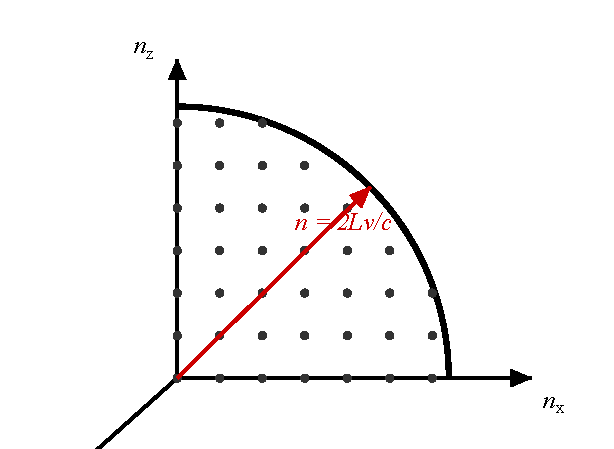
\includegraphics[width=0.5\linewidth]{Capitulo 5/Figuras/ConteoModos.pdf}
                \caption{Conteo de los modos de la cavidad. Cada terna de enteros no negativos $(n_{x},n_{y},n_{z})$ etiqueta un modo, y los que tienen frecuencia menor que $\nu$ llenan el octante de radio $n = 2L\nu/c$, de manera que su número es el volumen de ese octante.}
                \label{fig:ConteoModos}
            \end{figure}

            En \eqref{eq:DensidadModos} está ya contenida toda la dificultad. El número de maneras distintas en que el campo puede oscilar dentro de la cavidad crece como el cuadrado de la frecuencia y no tiene cota superior: por muy alta que sea la frecuencia considerada, siempre caben más modos por encima de ella, y de hecho cada vez más. Este crecimiento sin límite es una consecuencia inevitable de que el campo electromagnético sea un medio continuo con infinitos grados de libertad, uno por cada punto del espacio, tal como discutimos en el capítulo de mecánica analítica al pasar de la cadena discreta al continuo. La densidad de modos es independiente de la forma de la cavidad y del material de las paredes, como exige el teorema de Kirchhoff, y puede demostrarse que el resultado \eqref{eq:DensidadModos} vale para cualquier recinto suficientemente grande comparado con la longitud de onda.

            Para obtener la densidad espectral de energía $\rho(\nu,T)$, es decir, la energía por unidad de volumen y de frecuencia, basta multiplicar el número de modos por la energía media que cada modo posee en equilibrio térmico,
            \begin{equation}\label{eq:EstructuraRho}
                \rho(\nu,T) = g(\nu)\,\overline{\varepsilon}(\nu,T) = \frac{8\pi\nu^{2}}{c^{3}}\,\overline{\varepsilon}(\nu,T).
            \end{equation}
            Este es el único punto en el que la electrodinámica no basta y hay que apelar a la física térmica, y vale la pena subrayarlo: toda la disputa entre la física clásica y la cuántica se reduce a qué se ponga en el lugar de $\overline{\varepsilon}$.

            La respuesta clásica es el teorema de equipartición, según el cual en equilibrio térmico cada grado de libertad cuadrático de un sistema posee una energía media $k_{B}T/2$. Un modo del campo es un oscilador armónico, y como tal tiene dos grados de libertad cuadráticos, la amplitud y su derivada temporal, o equivalentemente los términos eléctrico y magnético de la energía, de manera que
            \begin{equation}\label{eq:Equiparticion}
                \overline{\varepsilon}_{\text{clásica}} = 2\cdot\frac{1}{2}k_{B}T = k_{B}T,
            \end{equation}
            independientemente de la frecuencia del modo. Sustituyendo \eqref{eq:Equiparticion} en \eqref{eq:EstructuraRho} obtenemos la \textit{ley de Rayleigh y Jeans},
            \begin{equation}\label{eq:RayleighJeans}
                \boxed{\;\rho_{\text{RJ}}(\nu,T) = \frac{8\pi\nu^{2}}{c^{3}}\,k_{B}T .\;}
            \end{equation}

            Esta expresión, deducida por Lord Rayleigh en 1900 y corregida en su factor numérico por James Jeans en 1905, es correcta en el límite de frecuencias bajas y concuerda allí con los datos experimentales; pero es catastrófica en todo lo demás. Para verlo, calculemos la energía total contenida en la cavidad por unidad de volumen, que se obtiene integrando sobre todas las frecuencias,
            \begin{equation}\label{eq:CatastrofeIntegral}
                u_{\text{RJ}}(T) = \int_{0}^{\infty}\rho_{\text{RJ}}(\nu,T)\,d\nu = \frac{8\pi k_{B}T}{c^{3}}\int_{0}^{\infty}\nu^{2}\,d\nu = \frac{8\pi k_{B}T}{c^{3}}\left[\frac{\nu^{3}}{3}\right]_{0}^{\infty} = \infty .
            \end{equation}
            La integral diverge, y diverge además de la peor manera posible, pues lo hace en el extremo de frecuencias altas y como un cubo. Paul Ehrenfest bautizó este desastre en 1911 con el nombre que ha quedado: la \textit{catástrofe ultravioleta}.

            Lo que dice \eqref{eq:CatastrofeIntegral} no es un desacuerdo cuantitativo con el experimento sino un absurdo físico. La predicción clásica afirma que cualquier cavidad a cualquier temperatura por encima del cero absoluto contiene una cantidad infinita de energía, y que un cuerpo a temperatura ambiente debería emitir con intensidad creciente en el ultravioleta, en los rayos X y en los rayos gamma. Abrir un horno equivaldría a recibir una descarga letal de radiación. El origen del absurdo es transparente a la luz del cálculo que hemos hecho: hay infinitos modos de frecuencia arbitrariamente alta, según \eqref{eq:DensidadModos}, y la equipartición asigna a cada uno la misma energía $k_{B}T$, de manera que la energía total es infinita por la sencilla razón de que se está repartiendo una porción fija entre un número infinito de receptores. No hay ningún error en el cálculo: el conteo de modos es electrodinámica correcta y la equipartición es mecánica estadística correcta, de modo que la contradicción demuestra que alguna de las dos teorías es falsa fuera de su dominio.

            Por el otro extremo del espectro, Wilhelm Wien había propuesto en 1896 una fórmula empírica que ajustaba muy bien los datos de frecuencia alta,
            \begin{equation}\label{eq:LeyWien}
                \rho_{\text{W}}(\nu,T) = \alpha\,\nu^{3}\,e^{-\beta\nu/T},
            \end{equation}
            con $\alpha$ y $\beta$ constantes por determinar, pero que fallaba por completo en el infrarrojo, donde predice una densidad que tiende a cero mientras que las medidas de Rubens y Kurlbaum en el laboratorio de Berlín mostraban un crecimiento lineal con la temperatura. La situación en octubre de 1900 era, pues, la siguiente: dos fórmulas, cada una correcta en la mitad del espectro y catastróficamente falsa en la otra mitad, y ninguna deducible de principios generales aceptables.

            Max Planck llevaba seis años trabajando en el problema desde una perspectiva termodinámica, estudiando no el campo sino los \textit{resonadores} materiales de las paredes, es decir, los osciladores cargados que absorben y emiten radiación y que mantienen el equilibrio térmico con ella. El 19 de octubre de 1900 presentó ante la Sociedad Física Alemana una fórmula de interpolación entre los dos regímenes conocidos, y en la noche del 7 de diciembre, tras semanas de lo que él mismo describió como el trabajo más intenso de su vida, encontró la manera de deducirla. El precio fue una hipótesis que le resultaba profundamente desagradable y que calificó, en una carta escrita años después, como \textit{un acto de desesperación}.

            \begin{Assumption}[Hipótesis cuántica de Planck]\label{sup:Planck}
                Un resonador material de frecuencia $\nu$ no puede poseer una energía arbitraria, sino únicamente un múltiplo entero de una cantidad elemental proporcional a su frecuencia,
                \begin{equation}\label{eq:HipotesisPlanck}
                    \varepsilon_{n} = n\,h\nu, \qquad n = 0,1,2,\ldots,
                \end{equation}
                donde $h$ es una constante universal.
            \end{Assumption}

            Es indispensable subrayar el alcance exacto de este supuesto, porque es el punto que el relato habitual distorsiona. \textbf{La cuantización \eqref{eq:HipotesisPlanck} se aplica a los osciladores mecánicos de las paredes de la cavidad y no al campo electromagnético}, que para Planck seguía siendo la onda continua de Maxwell, capaz de transportar cualquier cantidad de energía. Lo que está cuantizado es el intercambio: la materia solo puede ceder o recibir energía en paquetes de tamaño $h\nu$, del mismo modo que una máquina expendedora solo acepta monedas de cierto valor aunque el dinero en abstracto sea divisible. Planck fue explícito y reiterado en este punto durante años, y de hecho combatió la hipótesis del cuanto de luz de Einstein hasta bien entrada la década de 1910; en la carta de recomendación que en 1913 escribió para la admisión de Einstein en la Academia Prusiana, tras elogiar sin reservas su obra, pidió que no se le tuviese demasiado en cuenta el haber \textit{errado el blanco} con su hipótesis de los cuantos de luz.

            Podemos ahora calcular la energía media de un resonador bajo el supuesto \ref{sup:Planck}. Este es el único lugar del desarrollo en que necesitamos física estadística, y basta con el ingrediente más elemental de ella, el factor de Boltzmann, según el cual la probabilidad de que un sistema en equilibrio a temperatura $T$ se encuentre en un estado de energía $\varepsilon$ es proporcional a $e^{-\varepsilon/k_{B}T}$. La energía media es entonces el promedio pesado
            \begin{equation}\label{eq:MediaPlanck1}
                \overline{\varepsilon} = \frac{\displaystyle\sum_{n=0}^{\infty}\varepsilon_{n}\,e^{-\varepsilon_{n}/k_{B}T}}{\displaystyle\sum_{n=0}^{\infty}e^{-\varepsilon_{n}/k_{B}T}}
                = \frac{\displaystyle\sum_{n=0}^{\infty}n h\nu\,e^{-nh\nu/k_{B}T}}{\displaystyle\sum_{n=0}^{\infty}e^{-nh\nu/k_{B}T}} ,
            \end{equation}
            donde la diferencia esencial con el cálculo clásico es que las sumas son \textit{sumas} y no integrales, precisamente porque las energías permitidas forman un conjunto discreto.

            Para evaluarlas introduzcamos la abreviatura
            \begin{equation}\label{eq:VariableX}
                x \equiv e^{-h\nu/k_{B}T}, \qquad 0 < x < 1 ,
            \end{equation}
            de manera que $e^{-nh\nu/k_{B}T} = x^{n}$. El denominador es entonces una serie geométrica, cuya suma conocemos,
            \begin{equation}\label{eq:SerieGeometrica}
                Z \equiv \sum_{n=0}^{\infty}x^{n} = \frac{1}{1-x},
            \end{equation}
            convergente porque $x<1$. El numerador se obtiene de \eqref{eq:SerieGeometrica} mediante un truco que vale la pena registrar porque se usa constantemente: derivando la serie geométrica término a término respecto de $x$,
            \begin{equation}\label{eq:DerivadaSerie}
                \frac{d}{dx}\sum_{n=0}^{\infty}x^{n} = \sum_{n=0}^{\infty}n\,x^{n-1} = \frac{d}{dx}\left(\frac{1}{1-x}\right) = \frac{1}{(1-x)^{2}},
            \end{equation}
            y multiplicando ambos miembros por $x$ para restaurar la potencia,
            \begin{equation}\label{eq:SumaN}
                \sum_{n=0}^{\infty}n\,x^{n} = \frac{x}{(1-x)^{2}} .
            \end{equation}
            Sustituyendo \eqref{eq:SerieGeometrica} y \eqref{eq:SumaN} en \eqref{eq:MediaPlanck1}, el cociente de las dos series se simplifica bastante,
            \begin{equation}\label{eq:MediaPlanck2}
                \overline{\varepsilon} = h\nu\,\frac{\dfrac{x}{(1-x)^{2}}}{\dfrac{1}{1-x}}
                = h\nu\,\frac{x}{(1-x)^{2}}\cdot\frac{1-x}{1} = \frac{h\nu\,x}{1-x},
            \end{equation}
            donde se ha cancelado un factor $(1-x)$ entre el numerador y el denominador. Dividiendo ahora numerador y denominador por $x$, lo que equivale a multiplicar por $e^{+h\nu/k_{B}T}$,
            \begin{equation}\label{eq:MediaPlanck3}
                \boxed{\;\overline{\varepsilon}(\nu,T) = \frac{h\nu}{x^{-1}-1} = \frac{h\nu}{e^{h\nu/k_{B}T}-1} .\;}
            \end{equation}

            Antes de continuar merece la pena leer físicamente el resultado \eqref{eq:MediaPlanck3}, porque en él está la solución del problema. Cuando la frecuencia es baja, de manera que $h\nu \ll k_{B}T$, el exponente es pequeño y podemos desarrollar la exponencial en serie, $e^{y} \approx 1 + y$, con lo cual
            \begin{equation}\label{eq:LimiteBajaFrec}
                \overline{\varepsilon} \approx \frac{h\nu}{\left(1 + \dfrac{h\nu}{k_{B}T}\right)-1} = \frac{h\nu}{\dfrac{h\nu}{k_{B}T}} = k_{B}T,
            \end{equation}
            que es exactamente la equipartición clásica \eqref{eq:Equiparticion}. Los modos de frecuencia baja no notan la discretización, porque el escalón $h\nu$ entre niveles consecutivos es minúsculo comparado con la energía térmica disponible y la escalera parece una rampa. Cuando la frecuencia es alta, en cambio, $h\nu \gg k_{B}T$, la exponencial del denominador es enorme y podemos despreciar el uno frente a ella,
            \begin{equation}\label{eq:LimiteAltaFrec}
                \overline{\varepsilon} \approx h\nu\,e^{-h\nu/k_{B}T} \xrightarrow[\nu\to\infty]{} 0,
            \end{equation}
            de manera que la energía media cae exponencialmente en lugar de permanecer constante. La razón física es que un modo de frecuencia muy alta no puede excitarse en absoluto: para subir siquiera al primer escalón necesitaría una energía $h\nu$ mucho mayor que la que la agitación térmica puede proporcionarle, de modo que se queda congelado en su estado fundamental y no participa en el reparto de la energía. Esta congelación de los grados de libertad de frecuencia alta es lo que impide la catástrofe, y es el mismo mecanismo que explica por qué los calores específicos de los sólidos caen a cero a baja temperatura, como Einstein demostraría en 1907.

            Sustituyendo finalmente \eqref{eq:MediaPlanck3} en la estructura general \eqref{eq:EstructuraRho}, con la densidad de modos \eqref{eq:DensidadModos} que dedujimos de la electrodinámica, obtenemos la \textit{ley de radiación de Planck}, representada en la figura \ref{fig:EspectroCuerpoNegro} junto a las dos leyes que vino a reemplazar,
            \begin{equation}\label{eq:LeyPlanck}
                \boxed{\;\rho(\nu,T) = \frac{8\pi\nu^{2}}{c^{3}}\cdot\frac{h\nu}{e^{h\nu/k_{B}T}-1} = \frac{8\pi h\nu^{3}}{c^{3}}\,\frac{1}{e^{h\nu/k_{B}T}-1} .\;}
            \end{equation}

            \begin{figure}[htbp]
                \centering
                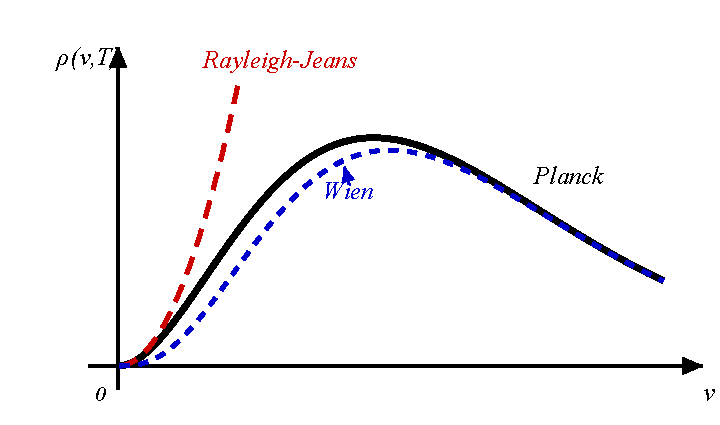
\includegraphics[width=0.72\linewidth]{Capitulo 5/Figuras/EspectroCuerpoNegro.pdf}
                \caption{Densidad espectral de la radiación de un cuerpo negro a temperatura fija. La ley de Rayleigh y Jeans crece sin límite con la frecuencia, la de Wien falla en el infrarrojo, y la de Planck coincide con cada una de ellas en su propio dominio de validez.}
                \label{fig:EspectroCuerpoNegro}
            \end{figure}

            Esta fórmula contiene a las dos que pretendía reconciliar. En el límite de frecuencia baja, sustituyendo \eqref{eq:LimiteBajaFrec},
            \begin{equation}\label{eq:RecuperaRJ}
                \rho \xrightarrow[h\nu\ll k_{B}T]{} \frac{8\pi\nu^{2}}{c^{3}}k_{B}T,
            \end{equation}
            que es exactamente la ley de Rayleigh y Jeans \eqref{eq:RayleighJeans}. En el límite de frecuencia alta, sustituyendo \eqref{eq:LimiteAltaFrec},
            \begin{equation}\label{eq:RecuperaWien}
                \rho \xrightarrow[h\nu\gg k_{B}T]{} \frac{8\pi h\nu^{3}}{c^{3}}\,e^{-h\nu/k_{B}T},
            \end{equation}
            que es la ley de Wien \eqref{eq:LeyWien} con las constantes empíricas identificadas como $\alpha = 8\pi h/c^{3}$ y $\beta = h/k_{B}$. Las dos constantes que Wien había tenido que ajustar a los datos quedan así expresadas en términos de constantes fundamentales, y esa es la primera de las razones por las cuales la fórmula de Planck se impuso de inmediato.

            La segunda razón es que la energía total ya no diverge. Integrando \eqref{eq:LeyPlanck} sobre todas las frecuencias y sustituyendo $y = h\nu/k_{B}T$, de donde $\nu = k_{B}Ty/h$ y $d\nu = k_{B}T\,dy/h$,
            \begin{equation}\label{eq:StefanPaso}
                u(T) = \int_{0}^{\infty}\frac{8\pi h\nu^{3}}{c^{3}}\frac{d\nu}{e^{h\nu/k_{B}T}-1}
                = \frac{8\pi h}{c^{3}}\left(\frac{k_{B}T}{h}\right)^{4}\int_{0}^{\infty}\frac{y^{3}}{e^{y}-1}\,dy,
            \end{equation}
            donde el factor $(k_{B}T/h)^{4}$ proviene de los tres factores del cubo más el que aporta el diferencial. La integral restante es un número puro cuyo valor es $\pi^{4}/15$, de manera que
            \begin{equation}\label{eq:StefanBoltzmann}
                u(T) = \frac{8\pi^{5}k_{B}^{4}}{15c^{3}h^{3}}\,T^{4} \equiv a\,T^{4},
            \end{equation}
            que es la ley que Josef Stefan había establecido experimentalmente en 1879 y que Boltzmann había deducido termodinámicamente en 1884. La ley de Planck no solo cura la divergencia sino que predice el valor numérico de la constante de Stefan a partir de $h$, $c$ y $k_{B}$, y el acuerdo con la medida fue lo que permitió a Planck obtener, en el mismo trabajo de 1900, la primera determinación razonablemente precisa de la constante que hoy lleva su nombre y, a partir de ella, del número de Avogadro y de la carga del electrón, años antes de que Millikan la midiera directamente.

            Queda por señalar la ironía histórica. La ley \eqref{eq:LeyPlanck} es correcta, y su deducción tal como la hemos presentado es esencialmente la que hoy se considera válida, pero la interpretación que Planck le dio no lo era. Él entendía la discretización como una propiedad de los resonadores materiales o incluso como un artificio de cálculo destinado a desaparecer en un tratamiento más fino, y dedicó la década siguiente a intentar deducir su propia fórmula sin recurrir a la hipótesis \ref{sup:Planck}. Nunca lo consiguió, porque no puede conseguirse. Planck abrió la puerta de la física cuántica convencido de que se trataba de una ventana que acabaría cerrándose, y fue Einstein quien, cinco años más tarde, comprendió que lo que había al otro lado era una casa entera.

    \subsection{La cuantización de la radiación según Einstein}

        El artículo que Albert Einstein envió a los \textit{Annalen der Physik} en marzo de 1905, el primero de los cuatro de aquel año prodigioso, lleva un título deliberadamente cauteloso: \textit{Sobre un punto de vista heurístico relativo a la producción y transformación de la luz}. Einstein lo describió en una carta a su amigo Conrad Habicht como el único de los cuatro que era \textit{muy revolucionario}, y tenía razón, porque mientras la relatividad especial modificaba la cinemática sin tocar el carácter ondulatorio de la luz, este trabajo afirmaba que la luz misma tiene estructura granular.

        De entrada hay que decir lo que no es este artículo. No es un trabajo sobre el efecto fotoeléctrico, al que dedica apenas dos páginas de las diecisiete, y no parte de la ley de Planck, de la que Einstein desconfiaba porque su deducción le parecía internamente inconsistente. \textbf{El argumento central es termodinámico y estadístico: Einstein calcula la entropía de la radiación en el régimen de Wien, la compara con la entropía de un gas ideal y demuestra que ambas tienen exactamente la misma dependencia con el volumen, de lo cual concluye que la radiación se comporta, en ese régimen, como si estuviera compuesta de partículas independientes.} Vamos a reproducir ese razonamiento paso a paso.

            Partimos de la ley de Wien \eqref{eq:LeyWien}, que Einstein toma como dato experimental firme en el dominio de frecuencia alta y que no requiere ninguna hipótesis sobre su origen,
            \begin{equation}\label{eq:WienPunto}
                \rho(\nu,T) = \alpha\nu^{3}e^{-\beta\nu/T} .
            \end{equation}
            El primer paso consiste en despejar la temperatura, porque la termodinámica relaciona la entropía con la energía a través de ella. Tomando logaritmos en \eqref{eq:WienPunto},
            \begin{equation}\label{eq:LogWien}
                \ln\rho = \ln\left(\alpha\nu^{3}\right) - \frac{\beta\nu}{T}
                \qquad\Longrightarrow\qquad
                \frac{\beta\nu}{T} = \ln\left(\alpha\nu^{3}\right) - \ln\rho = -\ln\frac{\rho}{\alpha\nu^{3}},
            \end{equation}
            de donde
            \begin{equation}\label{eq:UnoSobreT}
                \frac{1}{T} = -\frac{1}{\beta\nu}\ln\frac{\rho}{\alpha\nu^{3}} .
            \end{equation}

            Introducimos ahora la densidad de entropía espectral $\varphi(\rho,\nu)$, definida de manera que la entropía contenida en un volumen $V$ en el intervalo de frecuencias $d\nu$ sea $V\varphi\,d\nu$. La relación termodinámica fundamental, aplicada a volumen constante, establece que
            \begin{equation}\label{eq:RelacionTermo}
                \frac{\partial\varphi}{\partial\rho} = \frac{1}{T},
            \end{equation}
            de manera que sustituyendo \eqref{eq:UnoSobreT} tenemos una ecuación diferencial para $\varphi$,
            \begin{equation}\label{eq:EDOEntropia}
                \frac{\partial\varphi}{\partial\rho} = -\frac{1}{\beta\nu}\ln\frac{\rho}{\alpha\nu^{3}} .
            \end{equation}
            Integrémosla respecto de $\rho$. Recordando la primitiva $\int\ln(u)\,du = u\ln u - u$, y tratando $\nu$ como un parámetro,
            \begin{equation}\label{eq:IntegralEntropia}
                \varphi = -\frac{1}{\beta\nu}\int\ln\frac{\rho}{\alpha\nu^{3}}\,d\rho
                = -\frac{\rho}{\beta\nu}\left[\ln\frac{\rho}{\alpha\nu^{3}} - 1\right],
            \end{equation}
            donde la constante de integración se fija a cero exigiendo que la entropía se anule con la densidad de energía.

            Consideremos ahora una cantidad total de energía $E$ contenida en el volumen $V$, en el intervalo de frecuencias entre $\nu$ y $\nu + d\nu$, de manera que la densidad espectral es
            \begin{equation}\label{eq:RhoDeE}
                \rho = \frac{E}{V\,d\nu} .
            \end{equation}
            La entropía total de esa radiación es $S = V\varphi\,d\nu$, y sustituyendo \eqref{eq:IntegralEntropia} y \eqref{eq:RhoDeE},
            \begin{equation}\label{eq:EntropiaTotal}
                S = V\,d\nu\left(-\frac{E}{V\,d\nu\,\beta\nu}\right)\left[\ln\frac{E}{V\,d\nu\,\alpha\nu^{3}} - 1\right]
                = -\frac{E}{\beta\nu}\left[\ln\frac{E}{V\alpha\nu^{3}d\nu} - 1\right],
            \end{equation}
            donde el factor $V\,d\nu$ se ha cancelado con el que aparece en el denominador de la fracción exterior.

            Aquí llega el paso decisivo, y es de una sencillez desarmante. Preguntémonos cómo cambia esta entropía cuando la misma energía $E$ ocupa un volumen distinto, manteniendo fija la frecuencia. Escribiendo \eqref{eq:EntropiaTotal} para dos volúmenes $V$ y $V_{0}$ y restando,
            \begin{equation}\label{eq:DiferenciaEntropia1}
                S - S_{0} = -\frac{E}{\beta\nu}\left[\ln\frac{E}{V\alpha\nu^{3}d\nu} - \textcolor{red}{1} - \ln\frac{E}{V_{0}\alpha\nu^{3}d\nu} + \textcolor{red}{1}\right],
            \end{equation}
            donde los dos unos marcados en rojo se cancelan. La diferencia de logaritmos es el logaritmo del cociente, y en ese cociente se cancelan todos los factores comunes, es decir, $E$, $\alpha$, $\nu^{3}$ y $d\nu$, sobreviviendo únicamente los volúmenes,
            \begin{equation}\label{eq:DiferenciaEntropia2}
                S - S_{0} = -\frac{E}{\beta\nu}\ln\frac{V_{0}}{V} = \frac{E}{\beta\nu}\ln\frac{V}{V_{0}} .
            \end{equation}

            La expresión \eqref{eq:DiferenciaEntropia2} es el corazón del artículo de 1905, y su forma debió resultarle a Einstein inmediatamente reconocible, porque es idéntica a la que gobierna la expansión isoterma de un gas ideal.

            Consideremos, en efecto, un gas de $n$ partículas independientes encerradas en un volumen $V_{0}$, y preguntémonos cuál es la probabilidad de que en un instante dado todas ellas se encuentren simultáneamente dentro de una subregión de volumen $V$. Para una sola partícula, y suponiendo que su posición es uniformemente aleatoria, esa probabilidad es simplemente la razón de volúmenes $V/V_{0}$. Como las partículas son independientes, las probabilidades se multiplican, de manera que
            \begin{equation}\label{eq:ProbabilidadGas}
                W = \left(\frac{V}{V_{0}}\right)^{n} .
            \end{equation}
            El principio de Boltzmann, que Einstein escribe en la forma $S - S_{0} = k_{B}\ln W$ y que él mismo consideraba la relación más importante de toda la física estadística, da entonces
            \begin{equation}\label{eq:BoltzmannGas}
                S - S_{0} = k_{B}\ln\left(\frac{V}{V_{0}}\right)^{n} = n\,k_{B}\ln\frac{V}{V_{0}} .
            \end{equation}

            Al comparar \eqref{eq:DiferenciaEntropia2}, que se refiere a radiación, con \eqref{eq:BoltzmannGas}, que se refiere a un gas de partículas, se ve que ambas son proporcionales al logaritmo del cociente de volúmenes, y que la constante de proporcionalidad es $E/\beta\nu$ en un caso y $nk_{B}$ en el otro. Igualándolas,
            \begin{equation}\label{eq:IgualacionEinstein}
                \frac{E}{\beta\nu} = n\,k_{B}
                \qquad\Longrightarrow\qquad
                E = n\,k_{B}\beta\,\nu .
            \end{equation}
            Recordando que la constante $\beta$ de la ley de Wien vale $\beta = h/k_{B}$, según identificamos en \eqref{eq:RecuperaWien} al comparar con la ley de Planck, el producto $k_{B}\beta$ es exactamente $h$ y por tanto
            \begin{equation}\label{eq:ResultadoEinstein}
                \boxed{\;E = n\,h\nu .\;}
            \end{equation}

            Hay que ser muy preciso sobre lo que este cálculo demuestra y lo que no. No demuestra que la luz esté hecha de partículas en el sentido de pequeñas bolas que viajan por el espacio; demuestra que la entropía de la radiación monocromática, en el régimen de validez de la ley de Wien, depende del volumen exactamente como lo haría la de un gas de $n = E/h\nu$ entidades independientes. Einstein lo formuló con esa misma cautela en el enunciado que cierra su sección sexta: la radiación se comporta, desde el punto de vista termodinámico, \textit{como si} estuviera constituida por cuantos de energía independientes de magnitud $h\nu$. Que la conclusión sea estadística y no mecánica no la debilita; al contrario, la hace más robusta, porque no depende de ningún modelo sobre la estructura interna de esos cuantos.

            Dos observaciones completan el argumento. La primera es que la independencia mutua de los cuantos, que es lo que permite multiplicar las probabilidades en \eqref{eq:ProbabilidadGas}, solo se cumple en el régimen de Wien, es decir, cuando $h\nu\gg k_{B}T$ y el número de ocupación de cada modo es muy pequeño; en el régimen de Rayleigh y Jeans los cuantos no son independientes, y esa correlación, que Einstein analizó en 1909 al estudiar las fluctuaciones de energía de la radiación, es el primer indicio de lo que hoy llamamos estadística de Bose y del agrupamiento de fotones que Hanbury Brown y Twiss medirían medio siglo después. La segunda es que el paso de Planck a Einstein es un salto genuino y no una reformulación: Planck había cuantizado el intercambio de energía entre la materia y el campo, mientras que Einstein cuantiza el campo libre mismo, que puede propagarse durante millones de años a través del espacio vacío sin dejar de estar constituido por cuantos.

            Habiendo establecido la hipótesis, Einstein dedica las últimas páginas del artículo a extraer de ella consecuencias susceptibles de contraste experimental, y presenta tres.

            La primera es la regla de Stokes para la fotoluminiscencia, según la cual la luz reemitida por una sustancia fluorescente tiene siempre una frecuencia menor o igual que la de la luz incidente. En el marco clásico esta regla es un hecho empírico sin explicación; en el de Einstein es inmediata, pues un cuanto incidente de energía $h\nu$ no puede producir un cuanto emitido de energía mayor, ya que ello violaría la conservación de la energía en el proceso elemental,
            \begin{equation}\label{eq:Stokes}
                h\nu_{\text{emitido}} \leq h\nu_{\text{incidente}}
                \qquad\Longrightarrow\qquad
                \nu_{\text{emitido}} \leq \nu_{\text{incidente}} .
            \end{equation}

            La segunda es el efecto fotoeléctrico, descubierto por Hertz en 1887 de manera accidental mientras verificaba la existencia de las ondas de Maxwell y estudiado sistemáticamente por Lenard en 1902. El fenómeno consiste en que la luz que incide sobre un metal arranca electrones, y presenta tres rasgos que la teoría ondulatoria no puede explicar. El primero es la existencia de una frecuencia umbral por debajo de la cual no se emite ningún electrón por intensa que sea la iluminación, mientras que clásicamente una onda de intensidad suficiente debería acabar arrancándolos siempre. El segundo es que la energía de los electrones emitidos no depende de la intensidad sino de la frecuencia, cuando clásicamente la energía transportada por la onda es proporcional al cuadrado de la amplitud y por tanto a la intensidad. El tercero es la instantaneidad del proceso, pues los electrones aparecen sin retardo apreciable, mientras que un cálculo clásico del tiempo que tardaría un electrón en acumular la energía necesaria a partir de una onda débil arroja intervalos de minutos o de horas.

            La explicación de Einstein cabe en una línea. Si la luz consiste en cuantos de energía $h\nu$ y cada electrón absorbe uno solo de ellos, entonces la energía disponible para el electrón es $h\nu$, de la cual debe invertir una cantidad $W$, característica del metal y llamada \textit{función de trabajo}, en escapar de la superficie. La energía cinética máxima con que puede salir es, por tanto,
            \begin{equation}\label{eq:Fotoelectrico}
                \boxed{\;E_{\text{cin}}^{\max} = h\nu - W .\;}
            \end{equation}
            Las tres anomalías quedan explicadas simultáneamente. Existe una frecuencia umbral $\nu_{0} = W/h$ porque por debajo de ella el miembro derecho de \eqref{eq:Fotoelectrico} es negativo y el electrón no puede escapar; la energía depende de la frecuencia y no de la intensidad porque cada electrón interactúa con un solo cuanto, y aumentar la intensidad significa aumentar el número de cuantos y por tanto el número de electrones emitidos, no su energía individual; y el proceso es instantáneo porque no hay nada que acumular, ya que la transferencia ocurre de golpe.

            La predicción cuantitativa contenida en \eqref{eq:Fotoelectrico} es especialmente exigente y merece subrayarse, porque es la que decidió el asunto. Si se mide el potencial de frenado $V_{s}$ necesario para detener a los electrones más energéticos, se tiene $eV_{s} = E_{\text{cin}}^{\max}$ y por tanto
            \begin{equation}\label{eq:PotencialFrenado}
                V_{s} = \frac{h}{e}\,\nu - \frac{W}{e},
            \end{equation}
            de manera que al representar $V_{s}$ frente a $\nu$, como en la figura \ref{fig:Fotoelectrico}, debe obtenerse una recta cuya pendiente es $h/e$ y por tanto la misma para todos los metales, variando únicamente la ordenada en el origen. Robert Millikan dedicó diez años a intentar refutar esta predicción, en la que no creía, y en 1916 publicó la medida más cuidadosa que se había hecho del efecto, obteniendo rectas perfectas con una pendiente que daba $h = 6{,}57\times 10^{-34}\,\mathrm{J\,s}$, en excelente acuerdo con el valor deducido por Planck del espectro del cuerpo negro por un camino completamente distinto. Millikan reconoció que la ecuación de Einstein describía los datos con exactitud, pero siguió rechazando la hipótesis de los cuantos de luz que la sustentaba, lo cual ilustra hasta qué punto resultaba difícil de aceptar. El premio Nobel de 1921 le fue concedido a Einstein, de manera explícita, por el descubrimiento de la ley del efecto fotoeléctrico y no por la relatividad.

            \begin{figure}[htbp]
                \centering
                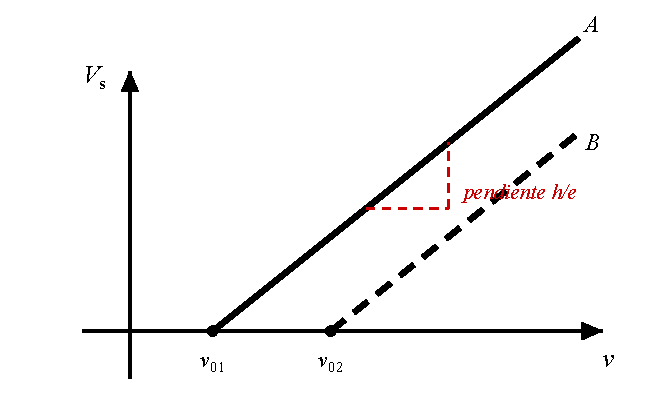
\includegraphics[width=0.62\linewidth]{Capitulo 5/Figuras/Fotoelectrico.pdf}
                \caption{Potencial de frenado frente a la frecuencia de la luz incidente para dos metales distintos. La predicción de Einstein es que las dos rectas sean paralelas, con pendiente $h/e$ común, y que solo difieran en la frecuencia umbral.}
                \label{fig:Fotoelectrico}
            \end{figure}

            La tercera consecuencia es la fotoionización, para la cual Einstein predice que la energía del cuanto debe ser al menos igual al potencial de ionización de la molécula, prediciendo también aquí un umbral en frecuencia.

    \subsection{El momento del cuanto: de Einstein 1917 al efecto Compton}

        Las tres consecuencias anteriores se refieren únicamente a la energía del cuanto. Un cuanto de luz con estructura de partícula debería poseer además \textit{momento lineal}, y esa segunda mitad del argumento tardó doce años en llegar y otros seis en comprobarse.

            En 1917 Einstein volvió sobre el problema del cuerpo negro con un artículo, \textit{Zur Quantentheorie der Strahlung}, que contiene dos aportaciones mayores. La primera es una deducción nueva y mucho más transparente de la ley de Planck, basada en el equilibrio detallado entre la materia y la radiación. Einstein considera moléculas con dos niveles de energía $\epsilon_{n}$ y $\epsilon_{m}$, con $\epsilon_{m}>\epsilon_{n}$, y postula tres procesos elementales: la absorción, con probabilidad proporcional a la densidad de radiación y coeficiente $B_{nm}$; la emisión estimulada por la radiación, con coeficiente $B_{mn}$; y la \textit{emisión espontánea}, con coeficiente $A_{mn}$, que ocurre sin necesidad de campo externo y que Einstein introduce por primera vez en este trabajo. En equilibrio, el número de transiciones en cada sentido debe igualarse,
            \begin{equation}\label{eq:BalanceDetallado}
                N_{n}B_{nm}\,\rho = N_{m}\left(B_{mn}\,\rho + A_{mn}\right),
            \end{equation}
            y usando la distribución de Boltzmann para las poblaciones, $N_{m}/N_{n} = e^{-(\epsilon_{m}-\epsilon_{n})/k_{B}T}$, se despeja la densidad espectral,
            \begin{equation}\label{eq:DespejeRho}
                \rho = \frac{A_{mn}/B_{mn}}{\dfrac{B_{nm}}{B_{mn}}e^{(\epsilon_{m}-\epsilon_{n})/k_{B}T} - 1} .
            \end{equation}
            Exigiendo que \eqref{eq:DespejeRho} se reduzca a la ley de Rayleigh y Jeans a temperatura muy alta se obtiene $B_{nm} = B_{mn}$, y comparando con la ley de Planck \eqref{eq:LeyPlanck} se obtienen de golpe las dos relaciones
            \begin{equation}\label{eq:RelacionesAB}
                \epsilon_{m}-\epsilon_{n} = h\nu
                \qquad\text{y}\qquad
                \frac{A_{mn}}{B_{mn}} = \frac{8\pi h\nu^{3}}{c^{3}} .
            \end{equation}
            La primera es la segunda regla de Bohr, que aquí no se postula sino que se deduce; la segunda fija la razón entre emisión espontánea y estimulada y es, cuarenta y tres años antes de Maiman, el fundamento teórico del láser, cuyo funcionamiento consiste precisamente en conseguir que la emisión estimulada domine sobre la espontánea mediante una inversión de población.

            La segunda aportación del artículo es la que aquí nos interesa. Einstein demuestra que para que las moléculas en equilibrio con la radiación de Planck mantengan la distribución de velocidades de Maxwell, no basta con contabilizar el intercambio de energía: hay que contabilizar también el intercambio de \textit{momento}, y los procesos elementales deben ser \textit{direccionales}. Si una molécula emite una energía $h\nu$, debe retroceder con un momento
            \begin{equation}\label{eq:MomentoCuanto}
                p = \frac{h\nu}{c} = \frac{h}{\lambda} = \hbar k,
            \end{equation}
            en una dirección bien definida, y no emitir una onda esférica que no produciría retroceso neto alguno. La conclusión de Einstein es tajante: la radiación saliente en forma de ondas esféricas no existe en los procesos elementales. Lo que llamamos onda esférica es la distribución de probabilidad de la dirección de emisión, no la emisión misma.

            El propio Einstein señala la incomodidad que le producía el resultado, en una frase que anticipa medio siglo de debate: \textit{la debilidad de la teoría radica en que deja la duración y la dirección de los procesos elementales al azar; no obstante, confío plenamente en que el camino elegido es el correcto}. La aleatoriedad que le incomodaba resultó ser irreducible, y la emisión espontánea que él tuvo que postular quedó explicada diez años más tarde por Dirac como emisión estimulada por las fluctuaciones del vacío que calcularemos más adelante en este capítulo.

            La comprobación directa de \eqref{eq:MomentoCuanto} llegó en 1923 de la mano de Arthur Compton, y fue el experimento que finalmente convenció a la comunidad. Compton hizo incidir rayos X de longitud de onda $\lambda$ sobre un blanco de grafito y midió la longitud de onda de la radiación dispersada en función del ángulo, encontrando que era \textit{mayor} que la incidente. Clásicamente esto es imposible: una onda electromagnética hace oscilar a los electrones a su propia frecuencia y estos reemiten a esa misma frecuencia, de manera que la longitud de onda no puede cambiar. Si en cambio la radiación consiste en cuantos con energía $h\nu$ y momento $h\nu/c$, el proceso es una colisión elástica entre dos partículas y el cuanto debe ceder parte de su energía al electrón, saliendo con menor frecuencia.

            \begin{figure}[htbp]
                \centering
                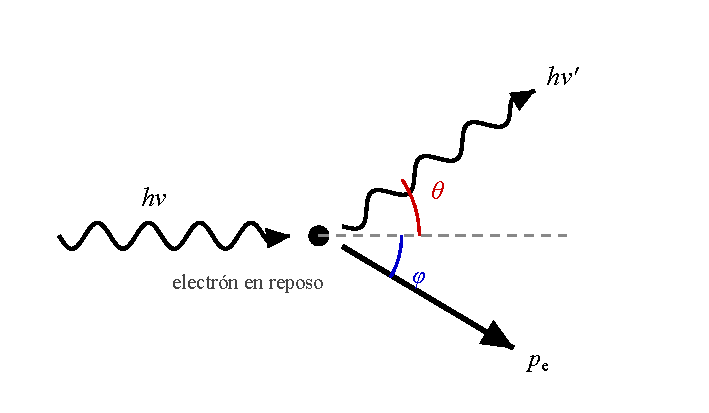
\includegraphics[width=0.72\linewidth]{Capitulo 5/Figuras/Compton.pdf}
                \caption{Geometría de la dispersión de Compton. El cuanto incidente cede parte de su energía y de su momento al electrón, que retrocede, y sale con una frecuencia menor y desviado un ángulo $\theta$.}
                \label{fig:Compton}
            \end{figure}

            El cálculo completo es un ejercicio de cinemática relativista. Sea un cuanto de frecuencia $\nu$ que incide sobre un electrón en reposo, de masa $m_{e}$, y que tras la colisión sale con frecuencia $\nu'$ formando un ángulo $\theta$ con la dirección incidente, mientras el electrón retrocede con momento $\mathbf{p}_{e}$ formando un ángulo $\varphi$ al otro lado, según la geometría de la figura \ref{fig:Compton}. La conservación del momento, proyectada sobre la dirección incidente y sobre la perpendicular, da
            \begin{align}
                \frac{h\nu}{c} &= \frac{h\nu'}{c}\cos\theta + p_{e}\cos\varphi, \label{eq:ComptonPx}\\
                0 &= \frac{h\nu'}{c}\sin\theta - p_{e}\sin\varphi, \label{eq:ComptonPy}
            \end{align}
            y la conservación de la energía, usando la expresión relativista para el electrón,
            \begin{equation}\label{eq:ComptonE}
                h\nu + m_{e}c^{2} = h\nu' + \sqrt{p_{e}^{2}c^{2}+m_{e}^{2}c^{4}} .
            \end{equation}

            El ángulo $\varphi$ del electrón no interesa, así que lo eliminamos. Despejando los términos que lo contienen en \eqref{eq:ComptonPx} y \eqref{eq:ComptonPy},
            \begin{equation}\label{eq:ComptonDespeje}
                p_{e}\cos\varphi = \frac{h\nu}{c} - \frac{h\nu'}{c}\cos\theta,
                \qquad
                p_{e}\sin\varphi = \frac{h\nu'}{c}\sin\theta,
            \end{equation}
            elevando ambas al cuadrado y sumándolas, con lo cual el miembro izquierdo se convierte en $p_{e}^{2}$ gracias a la identidad pitagórica,
            \begin{equation}\label{eq:ComptonSuma}
                p_{e}^{2} = \frac{h^{2}\nu^{2}}{c^{2}} - \frac{2h^{2}\nu\nu'}{c^{2}}\cos\theta + \frac{h^{2}\nu'^{2}}{c^{2}}\cos^{2}\theta + \frac{h^{2}\nu'^{2}}{c^{2}}\sin^{2}\theta,
            \end{equation}
            y usando de nuevo $\cos^{2}\theta+\sin^{2}\theta = 1$ para reunir los dos últimos términos,
            \begin{equation}\label{eq:ComptonPe2}
                p_{e}^{2}c^{2} = h^{2}\nu^{2} + h^{2}\nu'^{2} - 2h^{2}\nu\nu'\cos\theta .
            \end{equation}

            Trabajemos ahora la ecuación de la energía. Pasando $h\nu'$ al miembro izquierdo de \eqref{eq:ComptonE} y elevando al cuadrado para eliminar la raíz,
            \begin{equation}\label{eq:ComptonECuadrado}
                \left[h\left(\nu-\nu'\right) + m_{e}c^{2}\right]^{2} = p_{e}^{2}c^{2} + m_{e}^{2}c^{4},
            \end{equation}
            y desarrollando el cuadrado del binomio del miembro izquierdo,
            \begin{equation}\label{eq:ComptonDesarrollo}
                h^{2}\left(\nu-\nu'\right)^{2} + 2h\left(\nu-\nu'\right)m_{e}c^{2} + \textcolor{red}{m_{e}^{2}c^{4}} = p_{e}^{2}c^{2} + \textcolor{red}{m_{e}^{2}c^{4}},
            \end{equation}
            donde los dos términos marcados en rojo son idénticos y se cancelan. Desarrollando además el primer cuadrado,
            \begin{equation}\label{eq:ComptonPe2bis}
                p_{e}^{2}c^{2} = h^{2}\nu^{2} - 2h^{2}\nu\nu' + h^{2}\nu'^{2} + 2h\left(\nu-\nu'\right)m_{e}c^{2} .
            \end{equation}

            Tenemos ahora dos expresiones para la misma cantidad, \eqref{eq:ComptonPe2} y \eqref{eq:ComptonPe2bis}. Igualándolas, los términos $h^{2}\nu^{2}$ y $h^{2}\nu'^{2}$ aparecen en ambos miembros y se cancelan,
            \begin{equation}\label{eq:ComptonIgualacion}
                \textcolor{red}{h^{2}\nu^{2}} + \textcolor{red}{h^{2}\nu'^{2}} - 2h^{2}\nu\nu'\cos\theta = \textcolor{red}{h^{2}\nu^{2}} + \textcolor{red}{h^{2}\nu'^{2}} - 2h^{2}\nu\nu' + 2h\left(\nu-\nu'\right)m_{e}c^{2},
            \end{equation}
            y lo que queda, tras dividir todo por $2h$, es
            \begin{equation}\label{eq:ComptonCasi}
                -h\nu\nu'\cos\theta = -h\nu\nu' + \left(\nu-\nu'\right)m_{e}c^{2}
                \qquad\Longrightarrow\qquad
                h\nu\nu'\left(1-\cos\theta\right) = \left(\nu-\nu'\right)m_{e}c^{2} .
            \end{equation}
            Dividiendo ambos miembros por $\nu\nu'm_{e}c^{2}$,
            \begin{equation}\label{eq:ComptonFrecuencias}
                \frac{h}{m_{e}c^{2}}\left(1-\cos\theta\right) = \frac{\nu-\nu'}{\nu\nu'} = \frac{1}{\nu'} - \frac{1}{\nu},
            \end{equation}
            y multiplicando por $c$ para pasar de frecuencias a longitudes de onda, con $\lambda = c/\nu$,
            \begin{equation}\label{eq:Compton}
                \boxed{\;\Delta\lambda = \lambda' - \lambda = \frac{h}{m_{e}c}\left(1-\cos\theta\right) .\;}
            \end{equation}

            La fórmula \eqref{eq:Compton} tiene tres rasgos que la convierten en una prueba demoledora. El primero es que el corrimiento no depende de la longitud de onda incidente ni del material del blanco, sino únicamente del ángulo de observación, lo cual es una predicción rígida sin ningún parámetro ajustable. El segundo es que la constante que fija la escala,
            \begin{equation}\label{eq:LongitudCompton}
                \lambda_{C} = \frac{h}{m_{e}c} = 2{,}426\times 10^{-12}\,\mathrm{m},
            \end{equation}
            llamada \textit{longitud de onda de Compton del electrón}, combina la constante de Planck con la masa del electrón y la velocidad de la luz, de manera que medir la pendiente del corrimiento frente a $1-\cos\theta$ equivale a medir $h$ por un tercer camino independiente, y el valor obtenido coincidió con los de Planck y Millikan. El tercero es que el efecto es despreciable para luz visible, donde $\lambda_{C}/\lambda \sim 10^{-6}$, y solo se hace visible con rayos X, lo cual explica por qué nadie lo había observado antes.

            La comunidad se rindió ante este resultado, y no es difícil ver por qué. El efecto Compton es el experimento que cerró el debate, porque a diferencia del efecto fotoeléctrico, que admitía explicaciones semiclásicas alternativas en las que el campo permanecía continuo y era el átomo el que estaba cuantizado, aquí lo que se observa es una colisión entre dos objetos con energía y momento bien definidos. Compton recibió el premio Nobel en 1927, el mismo año en que Dirac cuantizó el campo electromagnético, y la palabra \textit{fotón}, acuñada por el químico Gilbert Lewis en 1926 para designar una entidad bastante distinta de la que hoy nombra, se impuso precisamente en esos años.

    \subsection{El fotón es indivisible: el experimento de Grangier, Roger y Aspect}

        Los argumentos anteriores establecen que la luz intercambia energía y momento en unidades discretas, pero ninguno de ellos obliga estrictamente a cuantizar el campo. Existe una escapatoria, y durante décadas hubo quien la defendió: se puede mantener un campo electromagnético clásico y continuo, y atribuir toda la discreción a la materia, es decir, a los átomos y a los detectores, que están cuantizados y por tanto solo pueden absorber energía en paquetes. Esta descripción, llamada \textit{semiclásica}, reproduce correctamente el efecto fotoeléctrico, el efecto Compton en su versión no relativista y buena parte de la óptica. Para demostrar que el campo mismo está cuantizado hace falta un experimento en el cual la predicción semiclásica y la cuántica difieran, y ese experimento tuvo que esperar hasta 1986.

            La idea es muy simple. Enviemos luz muy débil sobre un divisor de haz equilibrado, con un detector en cada salida, y preguntémonos con qué frecuencia ambos detectores se disparan a la vez. Una onda clásica, por débil que sea, se divide: una mitad se transmite y la otra se refleja, de manera que ambos detectores reciben señal simultáneamente y las coincidencias son frecuentes. Una partícula indivisible, en cambio, toma un camino o el otro y jamás los dos, de manera que las coincidencias deberían desaparecer por completo.

            Este argumento cualitativo se cuantifica mediante el \textit{parámetro de anticorrelación}
            \begin{equation}\label{eq:ParametroAlpha}
                \alpha \equiv \frac{P_{c}}{P_{t}\,P_{r}},
            \end{equation}
            donde $P_{t}$ y $P_{r}$ son las probabilidades de detección en los brazos transmitido y reflejado y $P_{c}$ la probabilidad de detección conjunta. Si las dos detecciones fuesen sucesos estadísticamente independientes se tendría $P_{c} = P_{t}P_{r}$ y por tanto $\alpha = 1$.

            El punto clave es el siguiente: cualquier teoría en la cual el campo sea una onda clásica, incluso si se le permite fluctuar aleatoriamente de la manera más caprichosa, predice
            \begin{equation}\label{eq:DesigualdadClasica}
                \alpha \geq 1 .
            \end{equation}
            La demostración se sigue de la desigualdad de Cauchy y Schwarz. En una descripción clásica, las probabilidades de detección son proporcionales a la intensidad instantánea $I(t)$ en cada brazo, y para un divisor equilibrado ambas son iguales a $I/2$; promediando sobre las fluctuaciones de la fuente, $P_{t} = P_{r} = \eta\overline{I}/2$ y $P_{c} = \eta^{2}\overline{I^{2}}/4$, de donde
            \begin{equation}\label{eq:AlphaClasico}
                \alpha = \frac{\eta^{2}\overline{I^{2}}/4}{\eta^{2}\overline{I}^{2}/4} = \frac{\overline{I^{2}}}{\overline{I}^{\,2}} \geq 1,
            \end{equation}
            porque la varianza $\overline{I^{2}} - \overline{I}^{\,2}$ de una cantidad real es siempre no negativa. La desigualdad \eqref{eq:AlphaClasico} no depende de ningún modelo concreto de la fuente: vale para cualquier distribución de intensidades positiva, y por tanto para toda teoría ondulatoria clásica imaginable. La teoría cuántica, en cambio, predice $\alpha = 0$ para un estado de un solo fotón, pues un único cuanto no puede ser detectado dos veces.

            El problema práctico es preparar un estado con \textit{un solo} fotón. Atenuar un láser no sirve, porque un haz coherente muy débil sigue siendo una superposición de estados de distinto número de fotones con estadística de Poisson, y para ella $\alpha = 1$ exactamente, indistinguible del límite clásico. Philippe Grangier, Gérard Roger y Alain Aspect resolvieron el problema en el Instituto de Óptica de Orsay recurriendo a una \textit{cascada radiativa atómica} \citep{Alan-Aspect}.

            La fuente es un haz atómico de calcio 40 excitado selectivamente por dos láseres hasta el nivel $4p^{2}\,{}^{1}S_{0}$. Desde allí el átomo decae en dos etapas sucesivas, emitiendo primero un fotón $\nu_{1}$ de $551{,}3$ nm, en el verde, al pasar al nivel intermedio $4s4p\,{}^{1}P_{1}$, y a continuación un segundo fotón $\nu_{2}$ de $422{,}7$ nm, en el violeta, al volver al fundamental $4s^{2}\,{}^{1}S_{0}$. La vida media del nivel intermedio es de unos $4{,}7$ ns, muy corta comparada con el intervalo medio entre cascadas sucesivas, que se ajusta mediante la densidad del haz atómico.

            El truco consiste en usar el primer fotón como \textit{heraldo}. La detección de $\nu_{1}$ en un fotomultiplicador, filtrado espectralmente para que solo acepte el verde, indica que el átomo se encuentra en el nivel intermedio y que por tanto se emitirá un fotón violeta en los próximos nanosegundos. Esa detección abre una ventana temporal electrónica de duración $w\approx 9$ ns durante la cual se observa el segundo canal. Dentro de esa ventana, y solo dentro de ella, se tiene la certeza de que el campo violeta contiene exactamente un fotón, que es precisamente el estado que ninguna fuente atenuada puede proporcionar.

            El fotón $\nu_{2}$ así preparado incide sobre un divisor de haz equilibrado, con un fotomultiplicador en la salida transmitida y otro en la reflejada, y un circuito de coincidencias registra las detecciones conjuntas dentro de la ventana. El esquema completo se muestra en la figura \ref{fig:Aspect}. En estas condiciones el parámetro \eqref{eq:ParametroAlpha} se determina a partir de los conteos medidos como
            \begin{equation}\label{eq:AlphaMedido}
                \alpha = \frac{N_{c}\,N_{1}}{N_{t}\,N_{r}},
            \end{equation}
            donde $N_{1}$ es el número de disparos del detector heraldo, $N_{t}$ y $N_{r}$ los de coincidencias dobles entre el heraldo y cada brazo, y $N_{c}$ el de coincidencias triples.

            \begin{figure}[htbp]
                \centering
                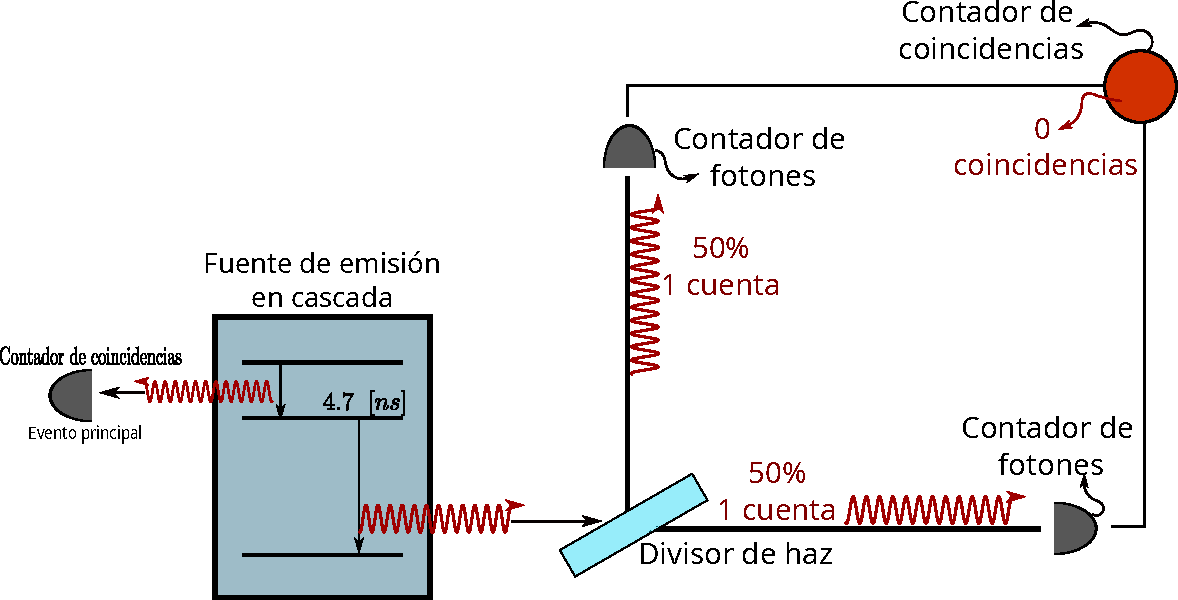
\includegraphics[width=0.9\linewidth]{Capitulo 5/Figuras/Aspect.pdf}
                \caption{Esquema experimental del estudio efectuado por Philippe Grangier, Gérard Roger y Alain Aspect en 1986. La detección del primer fotón de la cascada abre una ventana temporal durante la cual el segundo fotón, preparado en un estado de un solo cuanto, incide sobre un divisor de haz equilibrado con un detector en cada salida.}
                \label{fig:Aspect}
            \end{figure}

            La medida arrojó
            \begin{equation}\label{eq:ResultadoAspect}
                \alpha = 0{,}18 \pm 0{,}06,
            \end{equation}
            es decir, un valor que viola la cota clásica \eqref{eq:DesigualdadClasica} por trece desviaciones estándar. La desviación respecto del cero que predice la teoría cuántica ideal se explica por completo por las cascadas accidentales, esto es, por la probabilidad no nula de que un segundo átomo emita durante la ventana abierta por el primero, y en efecto el valor medido de $\alpha$ disminuye al reducir la duración de la ventana o la densidad del haz, tal como la teoría cuántica predice.

            El peso del argumento está en que no se trata de que el modelo ondulatorio ajuste peor los datos, sino de que \textbf{ninguna teoría en la que la luz sea una onda clásica, por complicada que sea su descripción estadística, puede producir un valor de $\alpha$ menor que uno}, porque ello exigiría que la varianza de una cantidad real fuese negativa. El experimento no refuta un modelo particular sino una clase entera de modelos, y esa es la razón por la cual es concluyente.

            El mismo trabajo contiene una segunda parte igual de importante y menos citada. Los autores tomaron exactamente la misma fuente de fotones individuales y, en lugar del divisor con dos detectores, la enviaron a un interferómetro de Mach y Zehnder, es decir, un montaje en el cual los dos caminos vuelven a recombinarse. Al variar la diferencia de camino observaron franjas de interferencia con una visibilidad del $98\%$. \textbf{El mismo objeto que en el primer montaje se niega tajantemente a dividirse en el divisor de haz, produce en el segundo un patrón de interferencia que exige que haya pasado por los dos brazos a la vez.} Esta es la formulación experimental más limpia que existe de la complementariedad de Bohr: no hay contradicción porque ambos comportamientos nunca se manifiestan en el mismo montaje, y cuál de los dos se observa depende de lo que el experimentador decida medir.

            Una advertencia final para evitar una confusión frecuente. El nombre de Alain Aspect se asocia habitualmente a los experimentos de 1981 y 1982 sobre las desigualdades de Bell, realizados con la misma fuente de cascada de calcio y por los que compartió el premio Nobel de 2022 con John Clauser y Anton Zeilinger; aquellos experimentos midieron correlaciones de polarización entre los dos fotones de la cascada y refutaron las teorías de variables ocultas locales. El experimento que hemos descrito aquí es posterior, de 1986, y su objeto es distinto: no la localidad, sino el carácter indivisible del cuanto de luz. Hay que mantenerlos separados porque responden a preguntas diferentes, aunque ambos usen la misma fuente y el mismo laboratorio.

            Con este resultado queda establecido lo que el título de esta sección anunciaba. La luz intercambia energía en cuantos, transporta momento en cuantos, y no puede dividirse por debajo del cuanto. Lo que resta del capítulo consiste en construir el formalismo que da cuenta de todo ello, y que no consiste en añadir partículas a la teoría electromagnética sino en cuantizar el propio campo, es decir, en aplicar al campo de Maxwell el mismo procedimiento canónico que el capítulo anterior aplicó a una partícula.

\section{Primera y segunda cuantización}

    La física del siglo XX nos legó dos revoluciones conceptuales que transformaron nuestra comprensión de la naturaleza: la mecánica cuántica y la teoría de campos. La óptica cuántica representa la confluencia de ambas tradiciones, aplicando el formalismo de la teoría cuántica de campos al caso particular de la radiación electromagnética. Antes de desarrollar ese formalismo hay que detenerse en qué significa exactamente cuantizar un sistema físico, porque la expresión \textit{segunda cuantización} es, con toda probabilidad, la más desafortunada del vocabulario de la física, y la confusión que genera vale la pena desarmarla de entrada.

    \subsection{Qué cuantiza la primera cuantización}

        El capítulo anterior desarrolló en detalle el procedimiento canónico. Se parte de un sistema mecánico clásico descrito por variables canónicas $q$ y $p$ que satisfacen el corchete de Poisson $\{q_{i},p_{j}\}=\delta_{ij}$, y se las promueve a operadores sobre un espacio de Hilbert sujetos a la relación de conmutación
        \begin{equation}\label{eq:PrimeraCuantizacion}
            \left[\hat{q}_{i},\hat{p}_{j}\right] = i\hbar\,\delta_{ij},
        \end{equation}
        que se obtiene del corchete clásico mediante la correspondencia de Dirac \cite{Dirac1930}. El objeto que resulta de este procedimiento es la función de onda $\psi(\mathbf{r},t)$, cuyo módulo al cuadrado da la densidad de probabilidad de hallar la partícula en cada punto.

        Seamos exactos sobre lo que se ha cuantizado aquí, porque el nombre induce a error. \textbf{Lo que la primera cuantización discretiza no es la posición ni el momento, que siguen teniendo espectro continuo, sino ciertas cantidades como la energía o el momento angular, y solo cuando las condiciones de frontera lo imponen.} Lo que realmente ocurre en \eqref{eq:PrimeraCuantizacion} es que las variables dinámicas dejan de ser números y pasan a ser operadores que no conmutan; la aparición de espectros discretos es una consecuencia de ese cambio de estatuto, no su definición. Un electrón libre, cuantizado en este sentido, tiene energía continua.

        La limitación decisiva del esquema es de otra índole y es puramente estructural: \textbf{el número de partículas es un dato fijo del problema y no una variable dinámica}. La función de onda de una partícula vive en $L^{2}(\mathbb{R}^{3})$, la de dos partículas en $L^{2}(\mathbb{R}^{6})$, y no existe ninguna operación dentro del formalismo que conecte ambos espacios. Si empezamos con una partícula, siempre tendremos una. Para la materia ordinaria a bajas energías esta restricción no molesta, porque los electrones de un átomo ni se crean ni se destruyen, pero para la luz es fatal: los fotones aparecen cuando un átomo emite y desaparecen cuando absorbe, de manera que el número de fotones es precisamente la variable que queremos describir.

    \subsection{Qué cuantiza la segunda cuantización}

        La segunda cuantización no consiste en cuantizar dos veces, y ahí está el origen de toda la confusión. \textbf{Se trata de aplicar el mismo y único procedimiento canónico \eqref{eq:PrimeraCuantizacion}, pero a un objeto distinto: no a las coordenadas de una partícula, sino a los grados de libertad de un campo.} El nombre histórico proviene de una circunstancia accidental, y es que el primer campo al que se aplicó el procedimiento fue la propia función de onda de Schrödinger, que ya era el resultado de una cuantización previa; de ahí que pareciera una segunda operación sobre lo mismo. Vista con perspectiva, la denominación correcta sería \textit{cuantización de campos}, y así la entenderemos aquí.

        El punto de partida es entonces un campo clásico $\phi(\mathbf{r},t)$ que obedece alguna ecuación de movimiento, como el campo electromagnético obedece las ecuaciones de Maxwell. Según demostramos en el capítulo de mecánica analítica al tratar los sistemas continuos, un campo es un sistema mecánico cuyo índice de grados de libertad, en lugar de ser un entero, es un punto del espacio, y posee por tanto una densidad lagrangiana, una densidad de momento canónico conjugado $\pi(\mathbf{r},t)$ y unos corchetes de Poisson a tiempos iguales. Aplicar a esos corchetes la correspondencia de Dirac da
        \begin{equation}\label{eq:SegundaCuantizacion}
            \left[\hat{\phi}(\mathbf{r},t),\,\hat{\pi}(\mathbf{r}',t)\right] = i\hbar\,\delta^{3}\!\left(\mathbf{r}-\mathbf{r}'\right),
        \end{equation}
        que es literalmente la misma prescripción \eqref{eq:PrimeraCuantizacion} con el índice discreto $i$ sustituido por la etiqueta continua $\mathbf{r}$ y la delta de Kronecker por la de Dirac. El campo deja de ser una función y pasa a ser un operador en cada punto del espacio.

        La consecuencia es que el espacio de estados ya no describe la configuración de un número fijo de partículas sino las excitaciones del campo, y debe acomodar cualquier número de ellas. Ese espacio, introducido por Fock \cite{Fock1932}, es la suma directa de los sectores con cada número de excitaciones,
        \begin{equation}\label{eq:EspacioFock}
            \mathcal{F} = \bigoplus_{n=0}^{\infty} \mathcal{H}^{(n)} = \mathcal{H}^{(0)} \oplus \mathcal{H}^{(1)} \oplus \mathcal{H}^{(2)} \oplus \cdots,
        \end{equation}
        donde $\mathcal{H}^{(0)} = \mathbb{C}$ es el sector de vacío, sin ninguna partícula, y $\mathcal{H}^{(n)}$ el de exactamente $n$ partículas. Los operadores de creación $\hat{a}^{\dagger}$ y aniquilación $\hat{a}$, que en el capítulo anterior servían para escalar los niveles de energía de un oscilador, adquieren aquí un significado nuevo: \textbf{conectan sectores de \eqref{eq:EspacioFock} con distinto número de partículas, y por tanto crean y destruyen partículas}. El número de partículas se convierte en el valor propio de un observable, el operador número, y deja de ser un parámetro externo.

        Resumamos el contraste en los tres puntos que realmente importan, porque son los que usaremos en el resto del capítulo.

        \begin{enumerate}
            \item \textit{Qué se promueve a operador.} En la primera cuantización, las coordenadas y los momentos de un número fijo de partículas. En la segunda, los valores del campo en cada punto del espacio y sus momentos conjugados.

            \item \textit{Qué papel juega la posición.} En la primera cuantización $\hat{\mathbf{r}}$ es un observable, es decir, un operador con espectro y valores propios. En la segunda, $\mathbf{r}$ deja de ser un observable y pasa a ser una simple etiqueta, un índice continuo que numera los grados de libertad del campo, exactamente como el subíndice $i$ numeraba las partículas de la cadena de osciladores. Este cambio de estatuto de la posición es la diferencia formal más profunda entre ambos esquemas.

            \item \textit{Qué es una partícula.} En la primera cuantización, el objeto de partida, que se supone dado. En la segunda, un \textbf{resultado}: la partícula es el cuanto de excitación del campo, es decir, el escalón elemental del espectro de un oscilador, y su existencia se deduce del álgebra $[\hat{a},\hat{a}^{\dagger}]=1$ en lugar de postularse.
        \end{enumerate}

        La frase que resume el capítulo entero es, entonces, la siguiente: en la primera cuantización se parte de partículas clásicas y se las hace cuánticas; en la segunda se parte de un campo clásico y se lo hace cuántico, y las partículas aparecen solas. \textbf{El fotón no se introducirá en ningún punto del desarrollo que sigue: aparecerá, sin haberlo invitado, como el entero que etiqueta los niveles de energía de cada modo del campo electromagnético.}

    \begin{figure}[htbp]
        \centering    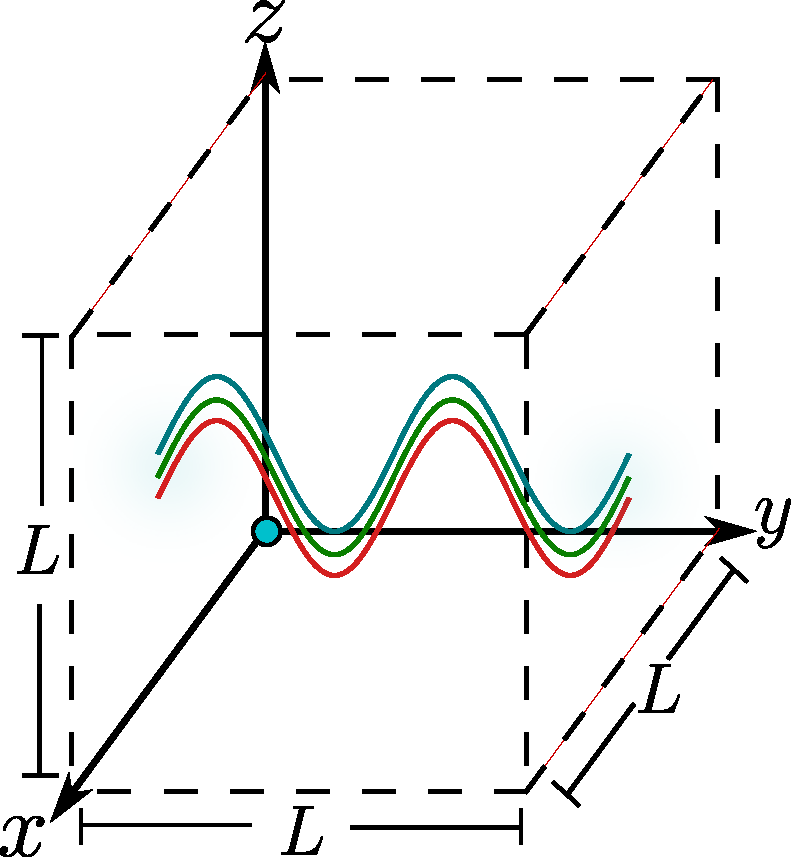
\includegraphics[width=0.45\textwidth]{Capitulo 5/Figuras/CavidadL.pdf}
        \caption{Campo eléctrico en todos sus modos confinado en una cavidad con paredes conductoras perfectas}
        \label{fig:cavidad}
    \end{figure}

   Para desarrollar la teoría cuántica del campo electromagnético, resulta conveniente trabajar con un sistema confinado en una región finita del espacio (ver figura \ref{fig:cavidad}). La cavidad resonante proporciona el escenario ideal: un recinto cerrado con paredes perfectamente conductoras que imponen condiciones de frontera bien definidas. Este modelo, aunque idealizado, captura la física esencial y permite un tratamiento matemático riguroso que luego puede generalizarse al espacio libre mediante un proceso de límite apropiado.

   Consideremos una cavidad cúbica de lado $L$, sin cargas ni corrientes en su interior. Las ecuaciones de Maxwell en el vacío toman la forma \cite{Jackson1999}
    \begin{align}
        \nabla \cdot \mathbf{E} &= 0, \\
        \nabla \cdot \mathbf{B} &= 0, \\
        \nabla \times \mathbf{E} &= -\frac{\partial \mathbf{B}}{\partial t}, \\
        \nabla \times \mathbf{B} &= \frac{1}{c^2}\frac{\partial \mathbf{E}}{\partial t},
    \end{align}
    donde $c = 1/\sqrt{\mu_0 \epsilon_0}$ es la velocidad de la luz.
    
    Para resolver estas ecuaciones, introducimos el potencial vector $\mathbf{A}(\mathbf{r}, t)$ mediante la relación $\mathbf{B} = \nabla \times \mathbf{A}$, que satisface automáticamente la condición $\nabla \cdot \mathbf{B} = 0$. La ley de Faraday implica entonces que $\nabla \times (\mathbf{E} + \partial\mathbf{A}/\partial t) = 0$, de donde podemos escribir
    \begin{equation}
        \mathbf{E} = -\nabla \Phi - \frac{\partial \mathbf{A}}{\partial t}
    \end{equation}
    para algún potencial escalar $\Phi$.
    
    Los potenciales $\mathbf{A}$ y $\Phi$ no están determinados unívocamente por los campos físicos $\mathbf{E}$ y $\mathbf{B}$; existe la libertad de gauge. Adoptamos el gauge de Coulomb, definido por la condición
    \begin{equation}
        \nabla \cdot \mathbf{A} = 0.
    \end{equation}
    
    Esta elección tiene una consecuencia importante. En ausencia de cargas, la ecuación $\nabla \cdot \mathbf{E} = 0$ junto con el gauge de Coulomb implica $\nabla^2 \Phi = 0$. En una cavidad cerrada, la única solución compatible con condiciones de frontera finitas es $\Phi = 0$. Los campos quedan entonces expresados exclusivamente en términos del potencial vector transversal:
    \begin{equation}
        \mathbf{E} = -\frac{\partial \mathbf{A}}{\partial t}, \quad \mathbf{B} = \nabla \times \mathbf{A}.
    \end{equation}
    
    Sustituyendo en la ecuación de Ampère-Maxwell y utilizando la identidad $\nabla \times (\nabla \times \mathbf{A}) = \nabla(\nabla \cdot \mathbf{A}) - \nabla^2 \mathbf{A}$, obtenemos la ecuación de onda
    \begin{equation}
        \nabla^2 \mathbf{A} - \frac{1}{c^2}\frac{\partial^2 \mathbf{A}}{\partial t^2} = 0.
    \end{equation}
    
    \section{Modos normales de la cavidad}
    
    Las paredes conductoras imponen que las componentes tangenciales del campo eléctrico se anulen en las fronteras. Buscamos soluciones mediante separación de variables, expandiendo el potencial vector en una serie de modos normales:
    \begin{equation}
        \mathbf{A}(\mathbf{r}, t) = \sum_{\mathbf{k},\lambda} q_{\mathbf{k},\lambda}(t) \, \mathbf{u}_{\mathbf{k},\lambda}(\mathbf{r}).
    \end{equation}
    
    Las funciones de modo $\mathbf{u}_{\mathbf{k},\lambda}(\mathbf{r})$ satisfacen la ecuación de Helmholtz $\nabla^2 \mathbf{u} + k^2 \mathbf{u} = 0$ junto con las condiciones de frontera. Para la cavidad cúbica, las soluciones involucran productos de funciones seno y coseno, y las condiciones de frontera cuantizan los componentes del vector de onda:
    \begin{equation}
        k_i = \frac{n_i \pi}{L}, \quad n_i = 0, 1, 2, 3, \ldots \quad (i = x, y, z).
    \end{equation}
    
    Cada vector $\mathbf{k}$ admite dos polarizaciones independientes, etiquetadas por $\lambda = 1, 2$. El gauge de Coulomb impone la condición de transversalidad $\mathbf{k} \cdot \hat{\boldsymbol{\epsilon}}_{\mathbf{k},\lambda} = 0$, de modo que los vectores de polarización son perpendiculares a la dirección de propagación. La frecuencia de cada modo está determinada por la relación de dispersión
    \begin{equation}
        \omega_{\mathbf{k}} = c\|\mathbf{k}\| = \frac{c\pi}{L}\sqrt{n_x^2 + n_y^2 + n_z^2}.
    \end{equation}
    
    Elegimos las funciones de modo normalizadas según
    \begin{equation}
        \int_V \mathbf{u}_{\mathbf{k},\lambda}(\mathbf{r}) \cdot \mathbf{u}_{\mathbf{k}',\lambda'}^*(\mathbf{r}) \, d^3r = \delta_{\mathbf{k},\mathbf{k}'}\delta_{\lambda,\lambda'},
    \end{equation}
    donde la integral se extiende sobre el volumen $V = L^3$ de la cavidad.
    
    Sustituyendo la expansión modal en la ecuación de onda y utilizando la ortogonalidad de las funciones de modo, encontramos que cada amplitud $q_{\mathbf{k},\lambda}(t)$ satisface
    \begin{equation}
        \ddot{q}_{\mathbf{k},\lambda}(t) + \omega_{\mathbf{k}}^2 q_{\mathbf{k},\lambda}(t) = 0.
    \end{equation}
    
    Esta es la ecuación de un oscilador armónico de frecuencia $\omega_{\mathbf{k}}$. Hemos llegado a un resultado fundamental: el campo electromagnético en una cavidad es dinámicamente equivalente a una colección infinita de osciladores armónicos independientes, uno por cada modo $(\mathbf{k}, \lambda)$.

    La energía total del campo electromagnético contenido en la cavidad es \cite{Jackson1999}
    \begin{equation}
        H = \frac{1}{2}\int_V \left(\epsilon_0 \|\mathbf{E}\|^2 + \frac{1}{\mu_0}\|\mathbf{B}\|^2\right) d^3r.
    \end{equation}
    
    Expresando los campos en términos del potencial vector y sustituyendo la expansión modal, el cálculo procede como sigue. Para el término eléctrico, usando $\mathbf{E} = -\partial\mathbf{A}/\partial t$:
    \begin{equation}
        \int_V \epsilon_0 \left\|\frac{\partial \mathbf{A}}{\partial t}\right\|^2 d^3r = \epsilon_0 \sum_{\mathbf{k},\lambda} |\dot{q}_{\mathbf{k},\lambda}|^2,
    \end{equation}
    donde hemos empleado la ortonormalidad de las funciones de modo.
    
    Para el término magnético, utilizamos que $\int_V \|\nabla \times \mathbf{u}_{\mathbf{k},\lambda}\|^2 d^3r = k^2 = \omega_{\mathbf{k}}^2/c^2$, lo cual conduce a
    \begin{equation}
        \int_V \frac{1}{\mu_0}\|\nabla \times \mathbf{A}\|^2 d^3r = \epsilon_0 \sum_{\mathbf{k},\lambda} \omega_{\mathbf{k}}^2 |q_{\mathbf{k},\lambda}|^2.
    \end{equation}
    
    Combinando ambas contribuciones, el Hamiltoniano total toma la forma
    \begin{equation}
        H = \frac{\epsilon_0}{2} \sum_{\mathbf{k},\lambda} \left(|\dot{q}_{\mathbf{k},\lambda}|^2 + \omega_{\mathbf{k}}^2 |q_{\mathbf{k},\lambda}|^2\right).
    \end{equation}
    
    Definiendo las variables canónicas $Q_{\mathbf{k},\lambda} = \sqrt{\epsilon_0} \, q_{\mathbf{k},\lambda}$ y $P_{\mathbf{k},\lambda} = \sqrt{\epsilon_0} \, \dot{q}_{\mathbf{k},\lambda}$, el Hamiltoniano adopta la forma estándar de una suma de osciladores armónicos:
    \begin{equation}
        H = \sum_{\mathbf{k},\lambda} \frac{1}{2}\left(P_{\mathbf{k},\lambda}^2 + \omega_{\mathbf{k}}^2 Q_{\mathbf{k},\lambda}^2\right).
    \end{equation}

    \subsection{Cuantización del campo electromagnético}

        Habiendo establecido que el campo electromagnético clásico en una cavidad es equivalente a un conjunto de osciladores armónicos, procedemos ahora a su cuantización. El procedimiento sigue el esquema canónico: promovemos las variables dinámicas a operadores y reemplazamos los corchetes de Poisson por conmutadores.

        Las variables canónicas $Q_{\mathbf{k},\lambda}$ y $P_{\mathbf{k},\lambda}$ se convierten en operadores hermitianos $\hat{Q}_{\mathbf{k},\lambda}$ y $\hat{P}_{\mathbf{k},\lambda}$ que satisfacen las relaciones de conmutación
        \begin{equation}
            [\hat{Q}_{\mathbf{k},\lambda}, \hat{P}_{\mathbf{k}',\lambda'}] = i\hbar \delta_{\mathbf{k},\mathbf{k}'}\delta_{\lambda,\lambda'},
        \end{equation}
        mientras que los conmutadores entre operadores del mismo tipo se anulan:
        \begin{equation}
            [\hat{Q}_{\mathbf{k},\lambda}, \hat{Q}_{\mathbf{k}',\lambda'}] = [\hat{P}_{\mathbf{k},\lambda}, \hat{P}_{\mathbf{k}',\lambda'}] = 0.
        \end{equation}

        Para el oscilador armónico cuántico, resulta conveniente introducir combinaciones lineales de los operadores de posición y momento que simplifican la estructura algebraica. Definimos el operador de aniquilación
        \begin{equation}
            \hat{a}_{\mathbf{k},\lambda} = \sqrt{\frac{\omega_{\mathbf{k}}}{2\hbar}}\hat{Q}_{\mathbf{k},\lambda} + \frac{i}{\sqrt{2\hbar\omega_{\mathbf{k}}}}\hat{P}_{\mathbf{k},\lambda}
        \end{equation}
        y el operador de creación como su adjunto hermitiano
        \begin{equation}
            \hat{a}^\dagger_{\mathbf{k},\lambda} = \sqrt{\frac{\omega_{\mathbf{k}}}{2\hbar}}\hat{Q}_{\mathbf{k},\lambda} - \frac{i}{\sqrt{2\hbar\omega_{\mathbf{k}}}}\hat{P}_{\mathbf{k},\lambda}.
        \end{equation}
        
        Para determinar el álgebra de estos operadores, calculamos su conmutador. Usando las relaciones de conmutación canónicas:
        \begin{align}
            [\hat{a}_{\mathbf{k},\lambda}, \hat{a}^\dagger_{\mathbf{k}',\lambda'}] &= \frac{\omega_{\mathbf{k}}}{2\hbar}[\hat{Q}_{\mathbf{k},\lambda}, \hat{Q}_{\mathbf{k}',\lambda'}] - \frac{i}{2\hbar}\sqrt{\frac{\omega_{\mathbf{k}}}{\omega_{\mathbf{k}'}}}[\hat{Q}_{\mathbf{k},\lambda}, \hat{P}_{\mathbf{k}',\lambda'}] \nonumber \\
            &\quad + \frac{i}{2\hbar}\sqrt{\frac{\omega_{\mathbf{k}'}}{\omega_{\mathbf{k}}}}[\hat{P}_{\mathbf{k},\lambda}, \hat{Q}_{\mathbf{k}',\lambda'}] + \frac{1}{2\hbar\sqrt{\omega_{\mathbf{k}}\omega_{\mathbf{k}'}}}[\hat{P}_{\mathbf{k},\lambda}, \hat{P}_{\mathbf{k}',\lambda'}].
        \end{align}
        
        Los conmutadores $[\hat{Q}, \hat{Q}]$ y $[\hat{P}, \hat{P}]$ se anulan. Utilizando $[\hat{Q}_{\mathbf{k},\lambda}, \hat{P}_{\mathbf{k}',\lambda'}] = i\hbar\delta_{\mathbf{k},\mathbf{k}'}\delta_{\lambda,\lambda'}$ y $[\hat{P}_{\mathbf{k},\lambda}, \hat{Q}_{\mathbf{k}',\lambda'}] = -i\hbar\delta_{\mathbf{k},\mathbf{k}'}\delta_{\lambda,\lambda'}$, obtenemos
        \begin{equation}
            [\hat{a}_{\mathbf{k},\lambda}, \hat{a}^\dagger_{\mathbf{k}',\lambda'}] = \frac{1}{2}\delta_{\mathbf{k},\mathbf{k}'}\delta_{\lambda,\lambda'} + \frac{1}{2}\delta_{\mathbf{k},\mathbf{k}'}\delta_{\lambda,\lambda'} = \delta_{\mathbf{k},\mathbf{k}'}\delta_{\lambda,\lambda'}.
        \end{equation}
        
        Por construcción, también se tiene $[\hat{a}_{\mathbf{k},\lambda}, \hat{a}_{\mathbf{k}',\lambda'}] = [\hat{a}^\dagger_{\mathbf{k},\lambda}, \hat{a}^\dagger_{\mathbf{k}',\lambda'}] = 0$. Estas son las relaciones de conmutación bosónicas características de los fotones.
        
        Las relaciones pueden invertirse para expresar los operadores de posición y momento en términos de los operadores de escalera:
        \begin{align}
            \hat{Q}_{\mathbf{k},\lambda} &= \sqrt{\frac{\hbar}{2\omega_{\mathbf{k}}}}\left(\hat{a}_{\mathbf{k},\lambda} + \hat{a}^\dagger_{\mathbf{k},\lambda}\right), \\
            \hat{P}_{\mathbf{k},\lambda} &= i\sqrt{\frac{\hbar\omega_{\mathbf{k}}}{2}}\left(\hat{a}^\dagger_{\mathbf{k},\lambda} - \hat{a}_{\mathbf{k},\lambda}\right).
        \end{align}
 
        Estas relaciones expresan que modos diferentes son dinámicamente independientes; cada par $(\mathbf{k}, \lambda)$ constituye un grado de libertad cuántico separado.

        Los campos electromagnéticos se promueven a operadores sustituyendo las amplitudes clásicas por operadores cuánticos. El operador de campo eléctrico resulta

        \begin{equation}
            \hat{E}(\mathbf{r}, t) = i\sum_{\mathbf{k},\lambda} \sqrt{\frac{\hbar\omega_{\mathbf{k}}}{2\epsilon_0 V}} \left(\hat{a}_{\mathbf{k},\lambda} e^{-i\omega_{\mathbf{k}} t} - \hat{a}^\dagger_{\mathbf{k},\lambda} e^{i\omega_{\mathbf{k}} t}\right) \hat{\boldsymbol{\epsilon}}_{\mathbf{k},\lambda} f_{\mathbf{k}}(\mathbf{r}),
        \end{equation}
        donde $f_{\mathbf{k}}(\mathbf{r})$ representa la dependencia espacial del modo y $V = L^3$ es el volumen de la cavidad.
        
        Análogamente, el operador de campo magnético es
        \begin{equation}
            \hat{B}(\mathbf{r}, t) = i\sum_{\mathbf{k},\lambda} \sqrt{\frac{\hbar}{2\epsilon_0\omega_{\mathbf{k}} V}} \left(\hat{a}_{\mathbf{k},\lambda} e^{-i\omega_{\mathbf{k}} t} - \hat{a}^\dagger_{\mathbf{k},\lambda} e^{i\omega_{\mathbf{k}} t}\right) (\mathbf{k} \times \hat{\boldsymbol{\epsilon}}_{\mathbf{k},\lambda}) g_{\mathbf{k}}(\mathbf{r}).
        \end{equation}
        
        Ambos operadores son hermitianos, como corresponde a observables físicos. La combinación particular de operadores de creación y aniquilación, con sus respectivas fases temporales, garantiza que $\hat{E}^\dagger = \hat{E}$ y $\hat{B}^\dagger = \hat{B}$.


    \subsection{El Oscilador Armónico Cuántico de la radiación y los Estados de Fock}
        
        La estructura matemática que hemos desarrollado conduce naturalmente al oscilador armónico cuántico, uno de los sistemas más importantes de toda la física teórica. En el contexto de la óptica cuántica, las excitaciones del oscilador armónico corresponden a los fotones.

        Partimos del Hamiltoniano de un modo individual, $\hat{H}_{\mathbf{k},\lambda} = \frac{1}{2}(\hat{P}^2 + \omega^2\hat{Q}^2)$, donde omitimos los subíndices para simplificar la notación. Sustituyendo las expresiones de $\hat{Q}$ y $\hat{P}$ en términos de $\hat{a}$ y $\hat{a}^\dagger$:
        \begin{equation}
            \hat{H} = \frac{1}{2}\left[-\frac{\hbar\omega}{2}(\hat{a}^\dagger - \hat{a})^2 + \omega^2 \cdot \frac{\hbar}{2\omega}(\hat{a} + \hat{a}^\dagger)^2\right].
        \end{equation}
        
        Expandiendo los cuadrados y simplificando:
        \begin{align}
            (\hat{a}^\dagger - \hat{a})^2 &= \hat{a}^\dagger\hat{a}^\dagger - \hat{a}^\dagger\hat{a} - \hat{a}\hat{a}^\dagger + \hat{a}\hat{a}, \\
            (\hat{a} + \hat{a}^\dagger)^2 &= \hat{a}\hat{a} + \hat{a}\hat{a}^\dagger + \hat{a}^\dagger\hat{a} + \hat{a}^\dagger\hat{a}^\dagger.
        \end{align}
        
        Al restar estas expresiones, los términos $\hat{a}^\dagger\hat{a}^\dagger$ y $\hat{a}\hat{a}$ se cancelan, quedando
        \begin{equation}
            (\hat{a} + \hat{a}^\dagger)^2 - (\hat{a}^\dagger - \hat{a})^2 = 2(\hat{a}\hat{a}^\dagger + \hat{a}^\dagger\hat{a}).
        \end{equation}
        
        Usando la relación de conmutación $[\hat{a}, \hat{a}^\dagger] = 1$, podemos escribir $\hat{a}\hat{a}^\dagger = \hat{a}^\dagger\hat{a} + 1$, de donde $\hat{a}\hat{a}^\dagger + \hat{a}^\dagger\hat{a} = 2\hat{a}^\dagger\hat{a} + 1$. El Hamiltoniano resulta
        \begin{equation}
            \hat{H} = \hbar\omega\left(\hat{a}^\dagger\hat{a} + \frac{1}{2}\right).
        \end{equation}
        
    \section{El operador número}
        
        Definimos el operador número como
        \begin{equation}
            \hat{N} \equiv \hat{a}^\dagger\hat{a}.
        \end{equation}
        
        Este operador cuenta el número de excitaciones (fotones) en el modo. En términos del operador número, el Hamiltoniano de cada modo se escribe
        \begin{equation}
            \hat{H}_{\mathbf{k},\lambda} = \hbar\omega_{\mathbf{k}}\left(\hat{N}_{\mathbf{k},\lambda} + \frac{1}{2}\right),
        \end{equation}
        y el Hamiltoniano total del campo electromagnético es la suma sobre todos los modos:
        \begin{equation}
            \hat{H} = \sum_{\mathbf{k},\lambda} \hbar\omega_{\mathbf{k}}\left(\hat{N}_{\mathbf{k},\lambda} + \frac{1}{2}\right).
        \end{equation}
        
        Para entender la acción de los operadores de escalera, calculamos sus conmutadores con el operador número. Usando la identidad $[AB, C] = A[B, C] + [A, C]B$:
        \begin{align}
            [\hat{N}, \hat{a}] &= [\hat{a}^\dagger\hat{a}, \hat{a}] = \hat{a}^\dagger[\hat{a}, \hat{a}] + [\hat{a}^\dagger, \hat{a}]\hat{a} = 0 - \hat{a} = -\hat{a}, \\
            [\hat{N}, \hat{a}^\dagger] &= [\hat{a}^\dagger\hat{a}, \hat{a}^\dagger] = \hat{a}^\dagger[\hat{a}, \hat{a}^\dagger] + [\hat{a}^\dagger, \hat{a}^\dagger]\hat{a} = \hat{a}^\dagger \cdot 1 + 0 = \hat{a}^\dagger.
        \end{align}
        
        Estas relaciones tienen una interpretación inmediata. Si $\ket{n}$ es un autoestado del operador número con autovalor $n$, entonces
        \begin{equation}
            \hat{N}(\hat{a}\ket{n}) = \hat{a}(\hat{N} - 1)\ket{n} = (n-1)(\hat{a}\ket{n}),
        \end{equation}
        lo que muestra que $\hat{a}\ket{n}$ es autoestado con autovalor $n-1$. Análogamente, $\hat{a}^\dagger\ket{n}$ es autoestado con autovalor $n+1$. Por esto $\hat{a}$ se llama operador de aniquilación (reduce el número de excitaciones en uno) y $\hat{a}^\dagger$ se llama operador de creación (aumenta el número en uno).

        Para determinar los autovalores permitidos del operador número, observamos primero que $\hat{N}$ es semidefinido positivo:
        \begin{equation}
            \bra{\psi}\hat{N}\ket{\psi} = \bra{\psi}\hat{a}^\dagger\hat{a}\ket{\psi} = \|\hat{a}\ket{\psi}\|^2 \geq 0.
        \end{equation}
        
        Por tanto, todos los autovalores son no negativos. Si existiera un autovalor no entero $n = m + \epsilon$ con $0 < \epsilon < 1$ y $m$ entero, la aplicación sucesiva del operador de aniquilación produciría eventualmente un autovalor negativo, lo cual es imposible. Concluimos que los autovalores deben ser enteros no negativos: $n = 0, 1, 2, 3, \ldots$
        
        El estado con $n = 0$ es el estado de vacío $\ket{0}$, caracterizado por
        \begin{equation}
            \hat{a}\ket{0} = 0.
        \end{equation}
        
        Los estados con $n$ fotones, llamados estados de Fock o estados número, se construyen aplicando el operador de creación repetidamente:
        \begin{equation}
            \ket{n} = \frac{(\hat{a}^\dagger)^n}{\sqrt{n!}}\ket{0}.
        \end{equation}
        
        El factor $1/\sqrt{n!}$ asegura la normalización $\braket{n|n} = 1$. Las acciones de los operadores de escalera sobre estos estados son
        \begin{align}
            \hat{a}\ket{n} &= \sqrt{n}\ket{n-1}, \\
            \hat{a}^\dagger\ket{n} &= \sqrt{n+1}\ket{n+1}.
        \end{align}
        
        La energía del estado con $n$ fotones en el modo $(\mathbf{k}, \lambda)$ es
        \begin{equation}
            E_n = \hbar\omega_{\mathbf{k}}\left(n + \frac{1}{2}\right).
        \end{equation}
        
        Los niveles de energía están igualmente espaciados, con separación $\hbar\omega_{\mathbf{k}}$ entre niveles consecutivos. Esta es precisamente la energía de un fotón de frecuencia $\omega_{\mathbf{k}}$, confirmando la interpretación corpuscular: cada excitación del campo corresponde a un fotón.

    \subsection{La energía del vacío cuántico}
        
        El término $\frac{1}{2}\hbar\omega_{\mathbf{k}}$ representa la energía de punto cero del modo, presente incluso cuando no hay fotones. La energía total del vacío electromagnético es
        \begin{equation}
            E_{\text{vacío}} = \frac{1}{2}\sum_{\mathbf{k},\lambda} \hbar\omega_{\mathbf{k}}.
        \end{equation}
        
        Esta suma diverge, pues hay infinitos modos. En la práctica, esta contribución infinita se elimina mediante técnicas de renormalización o redefiniendo el Hamiltoniano con ordenamiento normal, donde todos los operadores de creación se colocan a la izquierda de los de aniquilación.
        
        Sin embargo, la energía del vacío tiene consecuencias físicas observables. El efecto Casimir \cite{Casimir1948}, la fuerza atractiva entre dos placas conductoras paralelas en el vacío, es una manifestación directa de las fluctuaciones cuánticas del campo electromagnético.

    \subsection{Fluctuaciones del vacío}

        Dado que ya hemos descrito al campo eléctrico como una entidad que oscila de forma cuantizada de la misma manera que un oscilador armónico, podemos estudiar algunas de sus propiedades en el espacio número o de Fock. Para un modo estacionario único, el operador de campo eléctrico se escribe
        \begin{equation}\label{eq:CampoModoUnico}
            \hat{E}_{x}(z) = \mathcal{E}_{0}\sin(kz)\left(\hat{a} + \hat{a}^{\dagger}\right),
            \qquad
            \mathcal{E}_{0} = \sqrt{\frac{\hbar\omega}{\epsilon_{0}V}},
        \end{equation}
        donde $\mathcal{E}_{0}$ es la amplitud del campo asociada a un solo cuanto y no debe confundirse con la permitividad $\epsilon_{0}$ del vacío. Su valor esperado en un estado número se anula,
        \begin{equation}
            \left\langle \hat{E}_{x} \right\rangle_{n} = \mathcal{E}_{0}\sin(kz)\left[\bra{n}\hat{a}\ket{n} + \bra{n}\hat{a}^{\dagger}\ket{n}\right] = 0,
        \end{equation}
        porque $\hat{a}$ y $\hat{a}^{\dagger}$ conectan estados con números de fotones distintos y sus elementos diagonales son nulos. \textbf{Un estado con un número definido de fotones no tiene campo eléctrico medio}, resultado que a primera vista desconcierta y que expresa el hecho de que un estado número no posee fase definida, como se discutirá en detalle más adelante.

        Este resultado motiva a pensar en una incertidumbre intrínseca entre el número de fotones $n$ y el valor del campo, lo cual se evidencia calculando su conmutador,
        \begin{equation}
            \left[\hat{N}, \hat{E}_{x}\right] = \mathcal{E}_{0}\sin(kz)\left(\hat{a}^{\dagger} -\hat{a}\right)
            \quad\Longrightarrow\quad
            \Delta \hat{N}\,\Delta\hat{E}_{x} \geq \frac{1}{2}\mathcal{E}_{0}\left|\sin(kz)\right|\left|\left\langle\hat{a}^{\dagger} - \hat{a}\right\rangle\right|,
        \end{equation}
        donde la desigualdad es la relación de Robertson aplicada a este par de observables.

        El valor cuadrático medio, en cambio, no se anula,
        \begin{equation}
            \left\langle \hat{E}^{2}_{x}\right\rangle_{n} = \mathcal{E}_{0}^{2}\sin^{2}(kz)\,\bra{n}\left(\hat{a}^{\dagger}\right)^{2} + \hat{a}^{2} + \hat{a}^{\dagger}\hat{a} + \hat{a}\hat{a}^{\dagger}\ket{n} = 2\,\mathcal{E}_{0}^{2}\sin^{2}(kz)\left(n+ \frac{1}{2}\right),
        \end{equation}
        puesto que los dos primeros términos tienen valor esperado nulo y los dos últimos aportan $n$ y $n+1$ respectivamente. La incertidumbre del campo es entonces
        \begin{equation}
            \Delta \hat{E}_{x} = \sqrt{\left\langle \hat{E}^{2}_{x}\right\rangle - \left\langle \hat{E}_{x}\right\rangle^{2}} = \sqrt{2}\,\mathcal{E}_{0}\left|\sin(kz)\right|\sqrt{n+\frac{1}{2}} .
        \end{equation}

        Si nos fijamos en el estado de vacío $n = 0$, la incertidumbre del campo no se anula sino que vale $\mathcal{E}_{0}|\sin(kz)|/\sqrt{2}$, y este resultado es el que se conoce como la fluctuación del vacío cuántico del campo electromagnético. Es un pilar fundamental para el desarrollo de la electrodinámica cuántica, puesto que permite dar una explicación precisa y compatible con los resultados experimentales de diferentes fenómenos como lo son el corrimiento de Lamb, el efecto Casimir o la emisión espontánea de fotones \citep{Introd-QO}.
%Hablar 

\section{Los estados coherentes}

    Vamos a encontrar una familia de estados realmente importantes, primero encontrando cierta familia de estados especiales que a su vez son los autovalores del operador de aniquilación $\hat{a}$, sabemos que la mecánica cuántica debe producir los mismos resultados que la mecánica clásica en el caso límite en el que el oscilador armónico tiene una energía mucho mayor que la del cuanto de energía $\hbar \omega$.

    Por lo tanto, podemos plantear la siguiente pregunta: ¿es posible construir estados mecánicos cuánticos que conduzcan a predicciones físicas casi idénticas a las clásicas, al menos para un oscilador macroscópico? Veremos en este complemento que existen tales estados cuánticos: son superposiciones lineales coherentes de todos los estados. Los llamaremos \textit{estados cuasi-clásicos} o \textit{estados coherentes del oscilador armónico.}

    El problema que estamos considerando aquí es de gran interés general en la mecánica cuántica. Como bien se sabe en la mecánica cuántica muchos sistemas físicos pueden ser comparados con un oscilador armónico, al menos en una primera aproximación \cite{cohen1986quantum}. Para todos estos sistemas, es importante entender, en el marco de la mecánica cuántica, cómo pasar gradualmente del caso en el que los resultados dados por la aproximación clásica son suficientes al caso en el que los efectos cuánticos son preponderantes.

    La radiación electromagnética es un ejemplo muy importante de tal sistema. Dependiendo del experimento, revela su naturaleza mecánico cuántica o bien puede ser tratada clásicamente. Los estados coherentes de la radiación electromagnética fueron introducidos por Glauber y se utilizan actualmente en el campo de la óptica cuántica.\\

    Definimos los estados coherentes $\ket{\alpha}$ como los autoestados o estados propios del operador de aniquilación $\hat{a}$

    \begin{equation}
        \hat{a}\ket{\alpha} = \alpha\ket{\alpha}\;,
    \end{equation}

    podemos encontrar de muchas formas estos estados coherentes pero como conocemos bien los estados número $\ket{n}$ podemos encontrar los estados $\ket{\alpha}$ como una combinación lineal de los estados números pues estos conforman una base completa y ortonormal, en este orden de ideas tenemos

    \begin{equation}
        \ket{\alpha} = \sum_m C_m \ket{m}\;,
    \end{equation}

    \begin{equation}
        \hat{a}\ket{\alpha} = \sum_m C_m \sqrt{m}\ket{m-1} = \alpha \sum_n C_n \ket{n}\;,
    \end{equation}

    para el lado izquierdo de la ecuación vemos que se iguala al lado derecho cuando $m = n +1$ entonces tenemos la siguiente ecuación para los coeficientes de la expansión 
    
    \begin{equation}\label{eq:coefcnmahuno}
        C_{n+1}\sqrt{n + 1} = \alpha C_n \rightarrow C_{n+1} = \frac{\alpha}{\sqrt{n + 1}}C_n \;.
    \end{equation}

    La relación de recurrencia \ref{eq:coefcnmahuno} muestra un patrón en los coeficientes de la expansión, si evaluamos los primeros tres términos podemos ver dicho patrón:

    \begin{align*}
        C_1 = \frac{\alpha}{\sqrt{1}}C_0\;,\\
        C_2 = \frac{\alpha}{\sqrt{2}}C_1 = \frac{\alpha^2}{\sqrt{2\cdot 1}}C_0\;,\\
        C_3 = \frac{\alpha}{\sqrt{3}}C_2 = \frac{\alpha^3}{\sqrt{3\cdot 2\cdot 1}}C_0\;.
    \end{align*}

    Es fácil ver que el enésimo coeficiente se puede expresar en términos del primer coeficiente de la siguiente manera,

    \begin{equation}
        C_n = \frac{\alpha^n}{\sqrt{n!}}C_0\;.
    \end{equation}

    Vemos que cuando $C_0$ está fijo, es decir, es constante, el enésimo coeficiente también lo será esto implica que el estado $\ket{\alpha}$ es único o a lo mucho varía en una constante de proporcionalidad, para determinar el coeficiente $C_0$ vamos a aprovecharnos de que el estado $\ket{\alpha}$ debe estar normalizado, entonces tenemos la siguiente ecuación 

    \begin{equation}
        \sum_n |C_n|^2 = 1\;,
    \end{equation}

    \begin{equation}
        \sum_n \frac{|\alpha|^{2n}}{n!}|C_0|^2 = 1\;,
    \end{equation}

    pero podemos darnos cuenta que la suma no es más que una expansión en series de Taylor de un exponencial,

    \begin{equation}
        |C_0|^2 e^{|\alpha|^2} = 1 \rightarrow C_0 = e^{-|\alpha|^2/2}\;.
    \end{equation}

    Ahora, podemos determinar los estados coherentes como:

    \begin{equation}\label{eq:CoherentStates}
        \ket{\alpha} = e^{-|\alpha|^2/2}\sum_n \frac{\alpha^n}{\sqrt{n!}}\ket{n}\;.
    \end{equation}

    Vamos ahora a considerar el valor esperado del operador de campo eléctrico esto con el objetivo de hacer la comparación con los valores esperados de la mecánica clásica,

    \begin{equation}
        \hat{E}_x(\Vec{r},t) = i\left(\frac{\hbar \omega}{2\epsilon_0V}\right)^{1/2}\left[\hat{a}e^{i(\Vec{k}\cdot \Vec{r} - \omega t)} - \hat{a}^{\dagger}e^{-i(\Vec{k}\cdot\Vec{r} - \omega t)} \right]\;.
    \end{equation}

    Obtenemos entonces:

    \begin{equation}\label{eq:espEx}
        \bra{\alpha} \hat{E}_x \ket{\alpha} = i\left(\frac{\hbar \omega}{2\epsilon_0V}\right)^{1/2}\left[\alpha e^{i(\Vec{k}\cdot \Vec{r} - \omega t)} - \alpha^{*}e^{-i(\Vec{k}\cdot\Vec{r} - \omega t)} \right]\;.
    \end{equation}

    Ahora, como $\alpha$ puede ser, en general, un número complejo o real, lo podemos escribir en forma polar ($\alpha = |\alpha|e^{i\theta}$) e introducirlo a la ecuación \ref{eq:espEx}

    \begin{equation}
        \bra{\alpha} \hat{E}_x \ket{\alpha} = 2|\alpha|\left(\frac{\hbar \omega}{2\epsilon_0V}\right)^{1/2}\sin(\omega t - \Vec{k}\cdot \Vec{r} - \theta).
    \end{equation}

    ¿Esto tiene sentido? Si resolvemos la ecuación de onda del campo electromagnético con las condiciones de frontera de la cavidad, vemos que tanto el valor esperado cuántico en la base de los estados coherentes como los modos de oscilación de la radiación en una cavidad son semejantes.\\

    De la misma forma podemos calcular el valor esperado cuadrático del campo eléctrico, el cual da

    \begin{equation}
        \bra{\alpha}\hat{E}_x^2\ket{\alpha} = \frac{\hbar\omega}{2\epsilon_0 V}\left[1 + 4|\alpha|^2\sin^2(\omega t - \Vec{k}\cdot \Vec{r} - \theta) \right]\;.
    \end{equation}

    De esta forma podemos calcular la incertidumbre del campo eléctrico, teniendo en cuenta que está dada por $\Delta E_x = \sqrt{\langle \hat{E}_x^{2}\rangle - \langle \hat{E}_x\rangle^{2}}$, 

    \begin{equation}
        \Delta E_x = \left[\frac{\hbar\omega}{2\epsilon_0 V}\left[1 + 4|\alpha|^2\sin^2(\omega t - \Vec{k}\cdot \Vec{r} - \theta) \right] - 4|\alpha|^2\left(\frac{\hbar \omega}{2\epsilon_0V}\right)\sin^2(\omega t - \Vec{k}\cdot \Vec{r} - \theta) \right]^{1/2}\;,
    \end{equation}

    \begin{equation}
        \Delta E_x = \left(\frac{\hbar \omega}{2\epsilon_0 V} \right)^{1/2}\;,
    \end{equation}

    es la misma incertidumbre que para el del estado de vacío. Vemos que los estados coherentes tienen bien ganado su nombre de estados cuasi-clásicos pues el valor esperado del campo eléctrico coincide con su versión clásica pero sus fluctuaciones coinciden con las del vacío cuántico , es más si utilizamos los operadores de cuadratura tenemos la siguiente expresión:

    \begin{equation}
        \langle \left(\Delta\hat{X}_1\right)^2 \rangle_{\alpha} = \frac{1}{4} =  \langle \left(\Delta\hat{X}_2\right)^2 \rangle_{\alpha}.
    \end{equation}

    Por lo tanto, con respecto a los operadores de cuadratura de campo, los estados coherentes minimizan (de hecho, igualan) el producto de incertidumbre y muestran incertidumbres iguales, las del vacío, en cada cuadratura. De hecho, esta propiedad se puede utilizar como una definición alternativa para los estados coherentes. Considera tres operadores hermíticos, $\hat{A} , \hat{B} , \hat{C}$  que satisfacen la siguiente regla de conmutación

    \begin{equation}\label{eq:condiABC}
        \left[\hat{A} , \hat{B}\right] = i \hat{C}\;,
    \end{equation}

    del álgebra de operadores \cite{zettili2009quantum} se sabe bien que la relación de incertidumbre para dos observables cualesquiera $\hat{A}$ y $\hat{B}$ está dada por

    \begin{equation}
        \langle (\Delta\hat{A})^2 \rangle \langle (\Delta\hat{B})^2 \rangle \geq \frac{1}{4} \left|\langle [\hat{A},\hat{B}]\rangle \right|^{2}\;,
    \end{equation}

    utilizando la condición de conmutación \ref{eq:condiABC} se tiene entonces

    \begin{equation}
        \langle (\Delta\hat{A})^2 \rangle \langle (\Delta\hat{B})^2 \rangle \geq \frac{1}{4}\left|\langle \hat{C}\rangle\right|^{2}
    \end{equation}

    Los estados de mínima incertidumbre serán aquellos que convierten cumplen la igualdad, estos estados deben satisfacer la siguiente ecuación de autovalores \cite{merzbacher1998quantum}

    \begin{equation}
        \left[\hat{A} + \frac{i \langle \hat{C} \rangle}{2\langle (\triangle \hat{B})^2 \rangle} \hat{B} \right] \ket{\Psi} = \left[\langle \hat{A} \rangle + \frac{i \langle \hat{C} \rangle}{2\langle (\Delta \hat{B})^2 \rangle} \langle \hat{B} \rangle \right]\ket{\Psi}.
    \end{equation}


    Si utilizamos la relación de conmutación entre los operadores de cuadratura la ecuación de autovalores se convierte en la siguiente

    \begin{equation}
        \left[\hat{X}_1 + i\hat{X}_2 \right]\ket{\Psi} = \left[\langle \hat{X}_1 \rangle + i \langle \hat{X}_2 \rangle \right]\ket{\Psi}\;,
    \end{equation}

    donde surge \cite{gerry2005introductory} que el parámetro $\alpha$ está dado por $\alpha = \langle \hat{X}_1 \rangle + i \langle \hat{X}_2 \rangle $. Esta forma para el autovalor de los estados coherentes es bastante particular, pues por la forma que tiene podemos, a priori, especular que tenga algo que ver con el campo de Riemann-Silberstein pero la relación con dicho campo será tratada más adelante.
    
    ¿Qué interpretación física tiene $|\alpha|$? Con todo lo desarrollado hasta el momento, todo indica a que este está relacionado con la amplitud del campo (y por la forma que acabamos de encontrar para $\alpha$ lo podemos representar como un vector en el espacio de cuadratura complejo). Para ver esto, calculemos el valor esperado del número de cuantos de energía respecto a la base de estados coherentes

    \begin{equation}\label{eq:AlphaQuadrado}
        \langle n \rangle_{\alpha} = \bra{\alpha} \hat{n} \ket{\alpha} = \bra{\alpha} \hat{a}^{\dagger} \hat{a} \ket{\alpha} =\bra{\alpha} \alpha^* \alpha \ket{\alpha} = |\alpha|^2\;.
    \end{equation}

    Se puede ver entonces que $|\alpha|^2$ representa el valor esperado de cuantos de energía de la radiación, de esta misma forma podemos calcular las fluctuaciones del número de cuantos de la siguiente forma:

    \begin{equation}
        \bra{\alpha}\hat{n}^2\ket{\alpha} = \bra{\alpha}\hat{a}^{\dagger}\hat{a}\hat{a}^{\dagger}\hat{a}\ket{\alpha} = |\alpha|^4 + |\alpha|^2\;,
    \end{equation}

    \begin{equation}\label{eq:deltaEnexd}
        \Delta n = \sqrt{\langle \hat{n}^2 \rangle - \langle \hat{n} \rangle ^2} = |\alpha|\;.
    \end{equation}
    

    En este momento cabe preguntarse ¿qué está oscilando armónicamente? Si en el mundo macroscópico tenemos péndulos a pequeños ángulos o canicas oscilan en un pozo parabólico, en el contexto de la radiación ¿es el fotón el que está oscilando así? Para tratar de dar una solución a esto, primero desarrollemos la ecuación \ref{eq:CoherentStates} un poco más matemáticamente y luego veamos una representación gráfica tanto de los estados número como de los estados coherentes.\\

    Vamos a utilizar el teorema de desenlace \cite{sakurai1995modern}.

    \begin{myteo}\label{teo:Desenlace}
        Sean $\hat{A}$ y $\hat{B}$ dos operadores, que no necesariamente conmutan, se cumple que la regla de exponenciación de la suma de $\hat{A}$ y $\hat{B}$ es:

        \begin{equation}
            e^{\hat{A} + \hat{B}} = e^{\hat{A}}e^{\hat{B}}e^{-\frac{1}{2}[\hat{A},\hat{B}]} = e^{\hat{B}}e^{\hat{A}}e^{\frac{1}{2}[\hat{A},\hat{B}]}.
        \end{equation}

    \end{myteo}

    Vamos a definir el operador de desplazamiento $\hat{\mathcal{D}}$ el cual jugará un rol importante en la interpretación física de los estados coherentes. El operador de desplazamiento es

    \begin{equation}
        \hat{\mathcal{D}}(\alpha) = e^{\alpha\hat{a}^{\dagger} - \alpha^*\hat{a}},
    \end{equation}

    y utilizando el teorema \ref{teo:Desenlace} entonces queda:

    \begin{equation}
        \hat{\mathcal{D}} = e^{-\frac{1}{2}|\alpha|^2}e^{\alpha \hat{a}^{\dagger}}e^{-\alpha^*\hat{a}}.
    \end{equation}

    Podemos expandir cada uno de los exponenciales, exceptuando el primero, en series de Taylor y haremos que actúe sobre el estado de vacío $\ket{0}$.

    \begin{equation}
        e^{-\alpha^*\hat{a}} \ket{0} = \sum_{k=0}^{\infty}\frac{(-\alpha^*\hat{a})^k}{k!}\ket{0} = \ket{0}\;,
    \end{equation}

    \begin{equation}
        e^{\alpha\hat{a}^{\dagger}}\ket{0} = \sum_{n=0}^{\infty}\frac{\alpha^n}{n!}(\hat{a}^{\dagger})^n\ket{0} = \sum_{n=0}^{\infty}\frac{\alpha^n}{\sqrt{n!}}\ket{n}\;,
    \end{equation}

    En este orden de ideas, es fácil ver que aplicar el operador de desplazamiento sobre el estado de vacío $\ket{0}$ nos da origen a los estados coherentes $\ket{\alpha}$

    \begin{equation}
        \ket{\alpha} = \hat{\mathcal{D}}\ket{0}.
    \end{equation}

    Es decir, que los estados coherentes surgen al realizar desplazamientos de los estados de vacío, es decir, estados Gaussianos, los cuales oscilan como un oscilador armónico (esto se discutirá más a fondo en la siguiente subsección) ¿pero qué está oscilando? Comparemos un poco el comportamiento de estos estados respecto a los estados número ilustrados en la figura \ref{fig:EstadosNumero}.

    \begin{figure}[htbp]
        \centering
        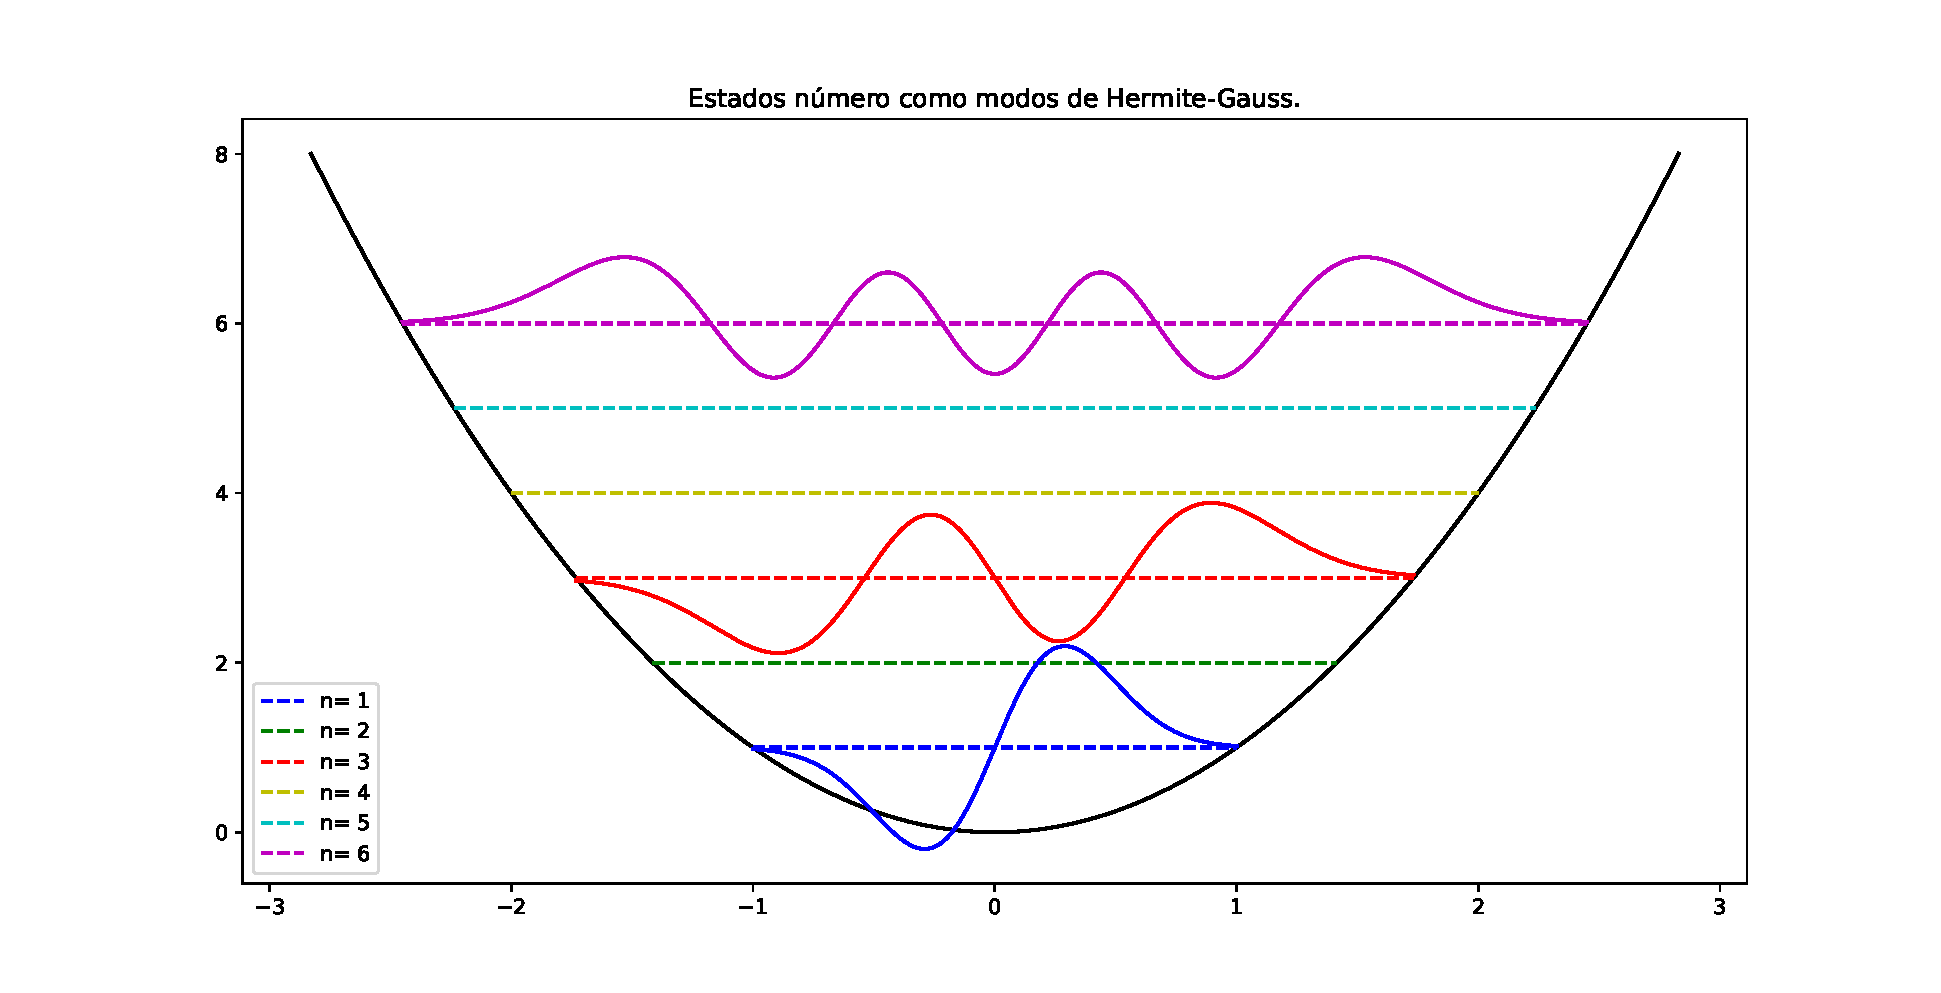
\includegraphics[width = \textwidth]{Capitulo 5/Figuras/EstadosNumero.pdf}
        \caption{Se representan gráficamente los primeros 6 niveles de energía para un oscilador harmónico cuántico, en este caso correspondiente al hamiltoniano del campo electromagnético. Para los niveles de energía; $1,3,6$ se ilustran estos estados en la base de posición, los cuales corresponden a las funciones de Hermite-Gauss.}
        \label{fig:EstadosNumero}
    \end{figure}

    Mientras que los estados número son estados estacionarios a lo largo de sus niveles de energía los estados coherentes evolucionan, en el sentido de que es un estado de vacío el cual está oscilando como un oscilador clásico pero como hemos visto, hay una relación de incertidumbre entre los operadores de campo eléctrico y magnético, no solo entre esos, sino entre los operadores de cuadratura, así que no es el fotón el que está oscilando armónicamente.\\

    Si nos remontamos a los orígenes de la mecánica cuántica, Albert Einstein hizo una gran contribución con su artículo \textit{la cuantización de la radiación} \cite{einstein20167} en la cual, en orden de que se cumpla la física cuántica de la radiación la energía de esta, de los fotones debe estar bien dirigida entonces podemos entender a los estados coherentes $\ket{\alpha}$ como los estados que me representan a nivel clásico las oscilaciones armónicas de la energía bien dirigida, estas oscilaciones se representan en la figura \ref{fig:EvolEstadosCoherentes}.

    \begin{figure}[htbp]
        \centering
        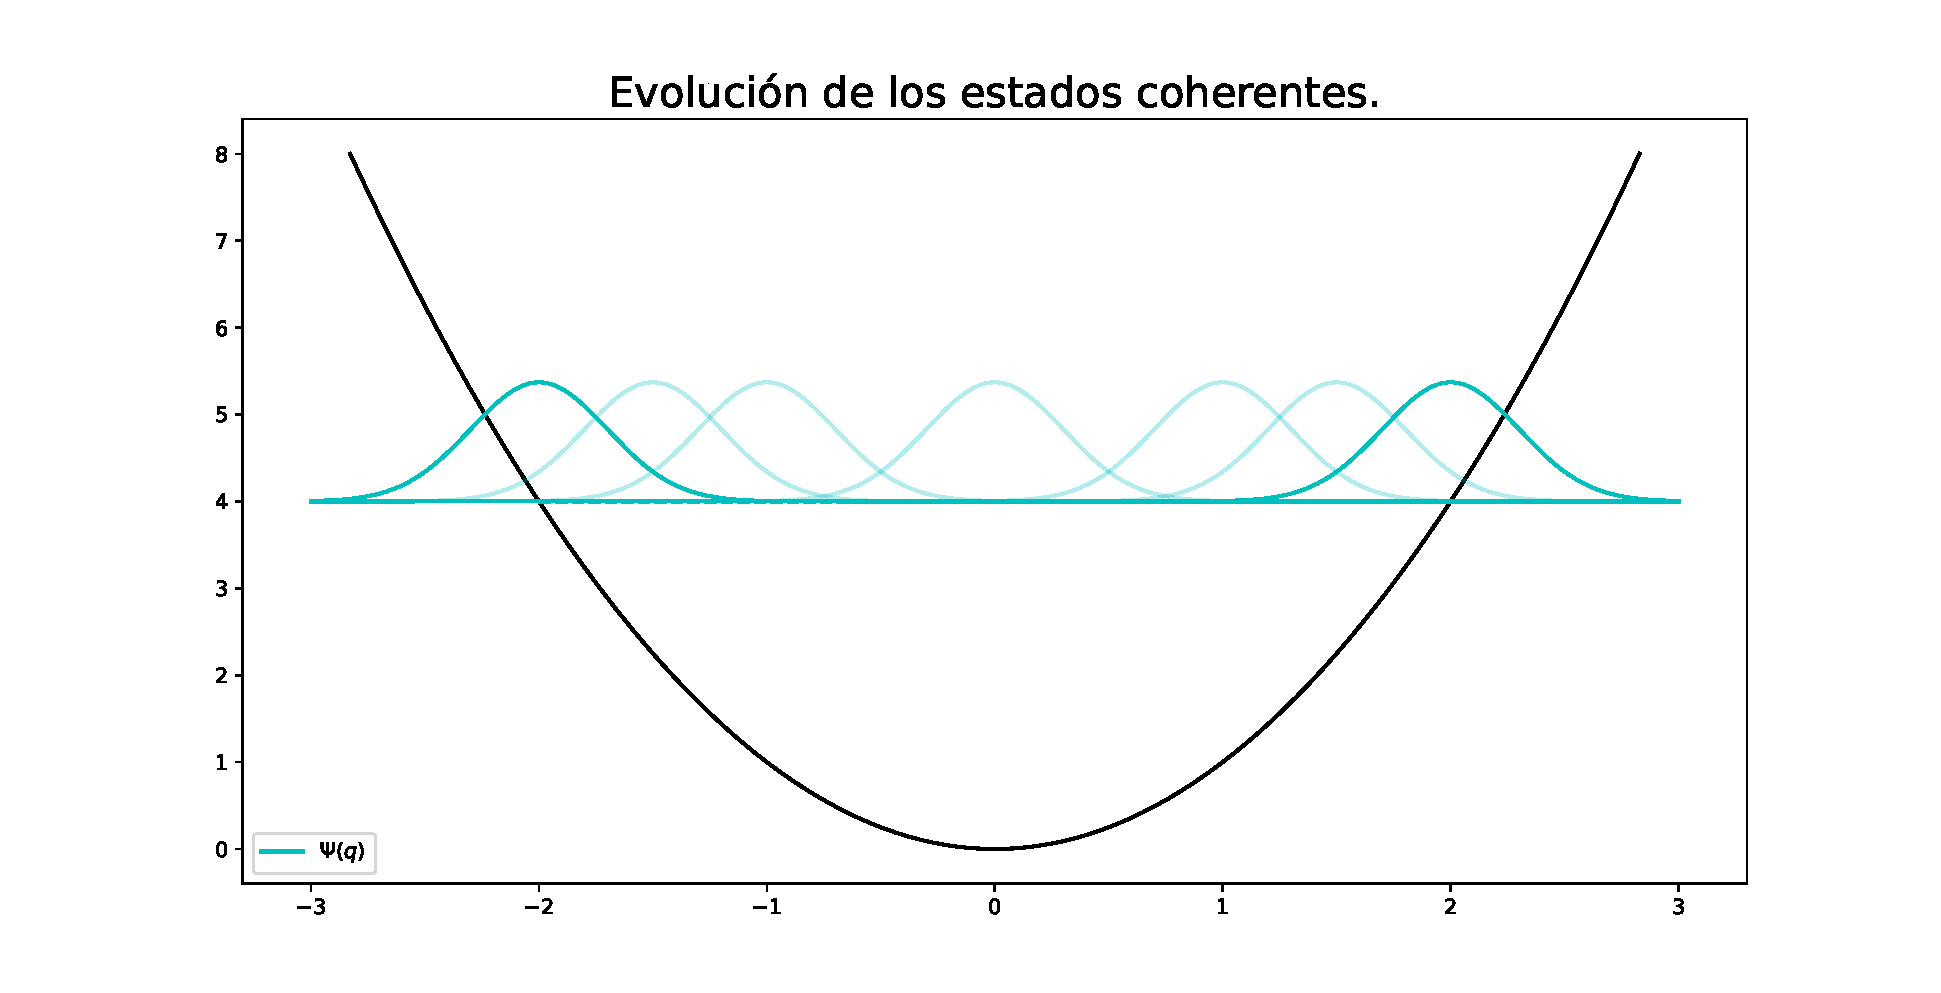
\includegraphics[width = \textwidth]{Capitulo 5/Figuras/EvolEstadosCoherentes.pdf}
        \caption{Los estados coherentes oscilan armónicamente a lo largo del potencial entre los puntos de retorno clásicos. Debido a la forma de estos estados, que sus autovalores con el operador de aniquilación correspondan a una representación compleja de los valores medios de los operadores cuadratura apunta a que físicamente estos estados representan la oscilación bien dirigida de la energía de la radiación.}
        \label{fig:EvolEstadosCoherentes}
    \end{figure}

    Esto se puede también ver un poco más matemáticamente representando estos estados en la base $q$ donde, recordemos, está relacionada con el operador cuadratura $\hat{X}_1$ de la siguiente forma,

    \begin{equation}
        \hat{q} = \sqrt{\frac{\hbar}{2\omega}}(\hat{a} + \hat{a}^{\dagger}) = \sqrt{\frac{2\hbar}{\omega}}\hat{X}_1\;,
    \end{equation}

    \begin{equation}
        \psi_{\alpha}(q) = \braket{q|\alpha} = \left(\frac{\omega}{\pi \hbar} \right)^{1/4}e^{-|\alpha|^2/2}e^{-\xi^{2}/2}\sum_{n=0}^{\infty}\frac{(\alpha /\sqrt{2})^n}{n!}H_n(\xi),
    \end{equation}

    donde $\xi = q\sqrt{\frac{\omega}{\hbar}}$ y $H_n$ son los polinomios de Hermite, mediante la generatriz de los polinomios de Hermite se puede reescribir esta ecuación de forma más compacta así:

    \begin{equation}
        \psi_{\alpha}(q) = \left(\frac{\omega}{\pi\hbar} \right)^{1/4}e^{-|\alpha|^2/2}e^{\xi^2/2}e^{-(\xi-\alpha/\sqrt{2})^2}\;.
    \end{equation}

    Aplicando la evolución temporal tenemos entonces

    \begin{equation}
        \psi_{\alpha}(q,t) = \left(\frac{\omega}{\pi\hbar} \right)^{1/4}e^{-|\alpha|^2/2}e^{\xi^2/2}e^{-(\xi-\alpha e^{-i\omega t}/\sqrt{2})^2}\;.
    \end{equation}
    
    \subsection{Distribución de probabilidad de los estados coherentes}

    Que las fluctuaciones ( o desviación estándar) del número de cuantos $n$ coincida con la magnitud de $\alpha$ nos da pistas de que tal vez la distribución de probabilidad que gobierna estos estados sea una estadística Poissionana \cite{swendsen2020introduction}. De hecho, cuando queremos medir el número de cuantos del campo, la probabilidad de detectar $n$ de estos es

    \begin{equation}\label{eq:PoissonForN}
        P_n = \left|\braket{n|\alpha}\right|^2 = e^{-|\alpha|^2}\frac{|\alpha|^{2n}}{n!} = e^{-\langle n \rangle}\frac{\langle n \rangle^{n}}{n!}.
    \end{equation}

    La ecuación \ref{eq:PoissonForN} es en realidad una densidad de probabilidad de tipo Poisson con valor medio igual a $\langle n \rangle$, podemos ver el comportamiento de esta distribución de probabilidad en la figura \ref{fig:HistogramaEstadosNumero}. 

    \begin{figure}[htbp]
        \centering
        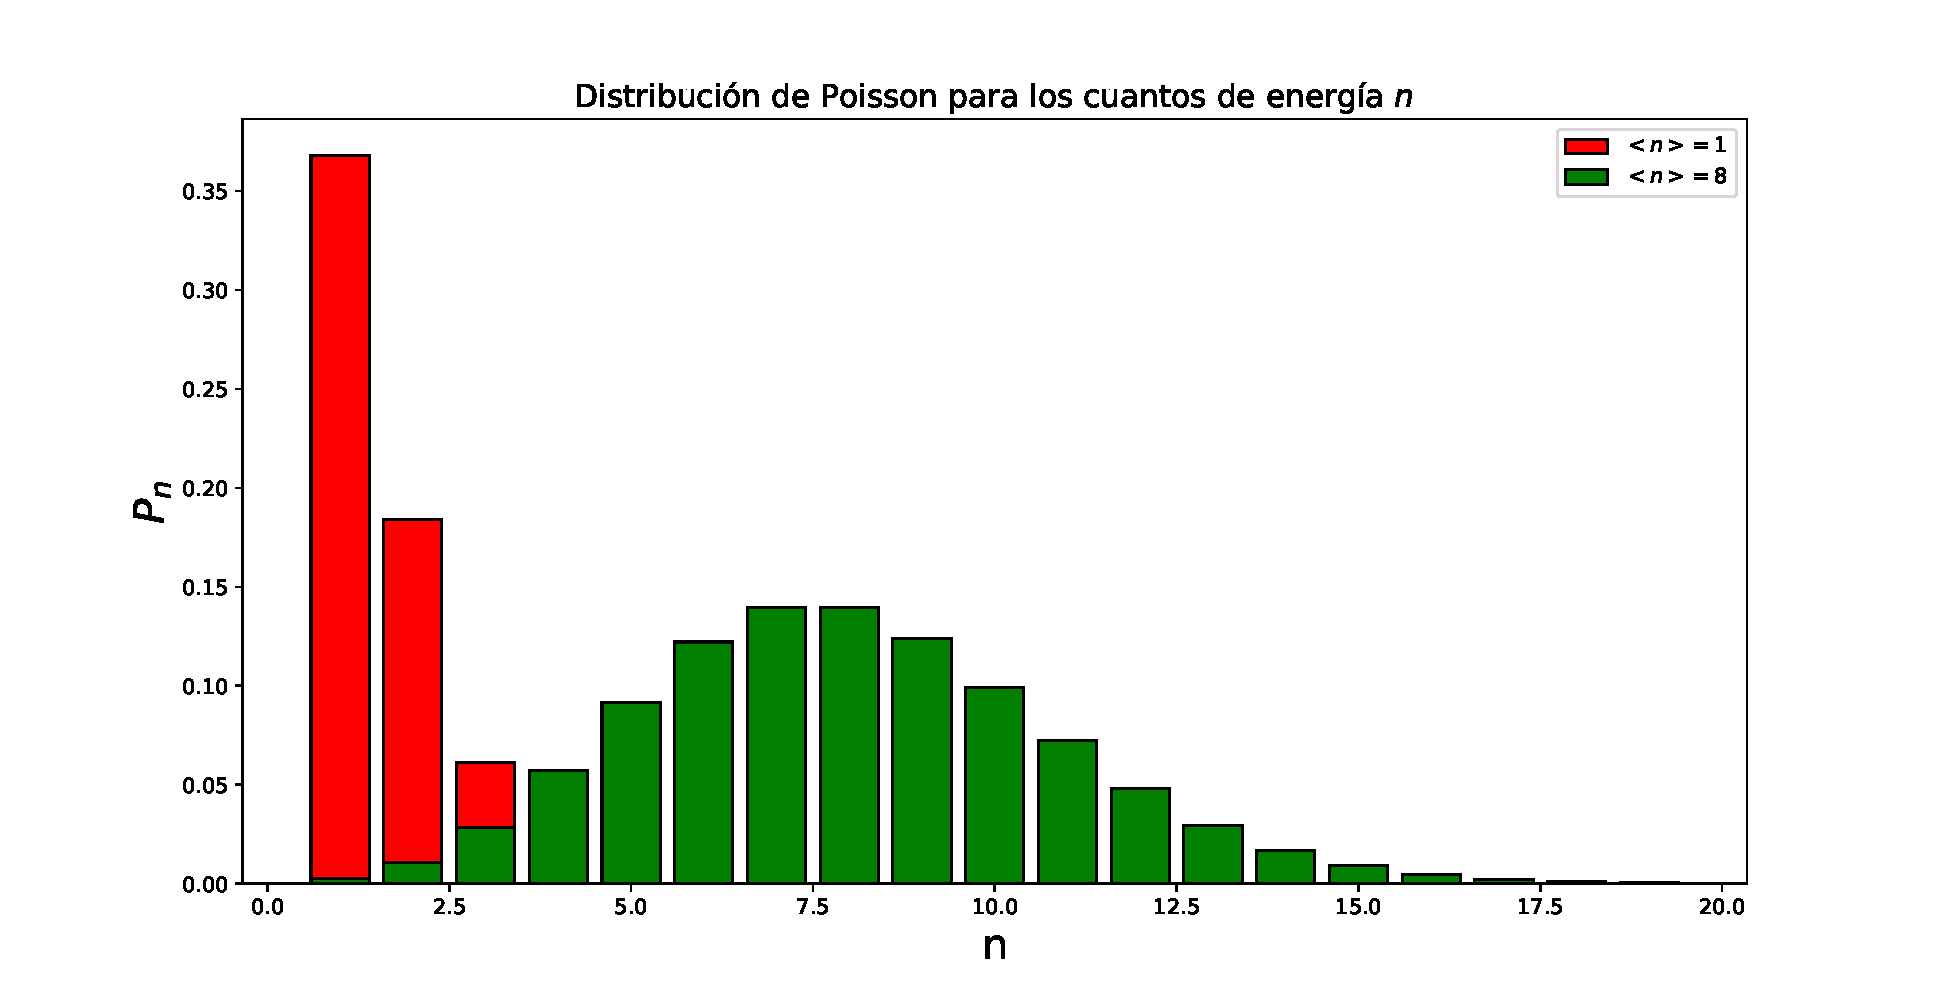
\includegraphics[width = \textwidth]{Capitulo 5/Figuras/HistogramasEstadoNumero.pdf}
        \caption{Densidad de probabilidad para los estados número coherentes.}
        \label{fig:HistogramaEstadosNumero}
    \end{figure}
    
    
    Ahora, veamos también la distribución de fase para los estados coherentes, aquí no entraremos en gran detalle sobre qué es la fase cuántica y cómo operar sobre esta (este tema se discutirá más adelante), gracias a que $\alpha$ es un número complejo este puede ser representado en forma polar $\alpha = |\alpha|e^{i\theta}$ pero como ya vimos este parámetro puede ser representado como $\alpha = \langle \hat{X}_1 \rangle + i \langle \hat{X}_2 \rangle$.
    

    Entonces la correspondiente distribución de fase \cite{gerry2005introductory} es

    \begin{equation}\label{eq:PdePhixd}
        P(\phi) = \frac{1}{2\pi}\left|\braket{\phi|\alpha}\right|^2 = \frac{1}{2\pi}e^{-|\alpha|^2}\left|\sum_{n=0}^{\infty}e^{in(\phi - \theta)} \frac{|\alpha|^{n}}{\sqrt{n!}}\right|^2.
    \end{equation}

    Para valores grandes de cuantos de energía o lo que es lo mismo para valores grandes de $|\alpha|^2$ la distribución de Poisson se aproximará a una Gaussiana:

    \begin{equation}
        e^{-|\alpha|^2} \frac{|\alpha|^{2n}}{n!} \approx \left(2\pi |\alpha|^2\right)^{-1/2} e^{\left[- \frac{(n-|\alpha|^2)^2}{2|\alpha|^2} \right]}
    \end{equation}

    de esta forma la ecuación \ref{eq:PdePhixd} se aproxima al a siguiente forma Gaussiana

    \begin{equation}
        P(\phi) \approx \left(\frac{2|\alpha|^2}{\pi}\right)^{1/2}e^{-2|\alpha|^2(\phi - \theta)^2}\;.
    \end{equation}

    Esta es una densidad de probabilidad Gaussiana cuyo pico se encuentra cuando $\phi = \theta$ y cuyo ancho, igual a $1/(2|\alpha|)$, es inversamente proporcional a $|\alpha|$, es decir, cuanto más grande es el valor medio de cuantos de energía más localizada está la distribución Gaussiana, esto se puede ver en la figura \ref{fig:DistriFaseCoherent}.\\

    \begin{figure}[htbp]
        \centering
        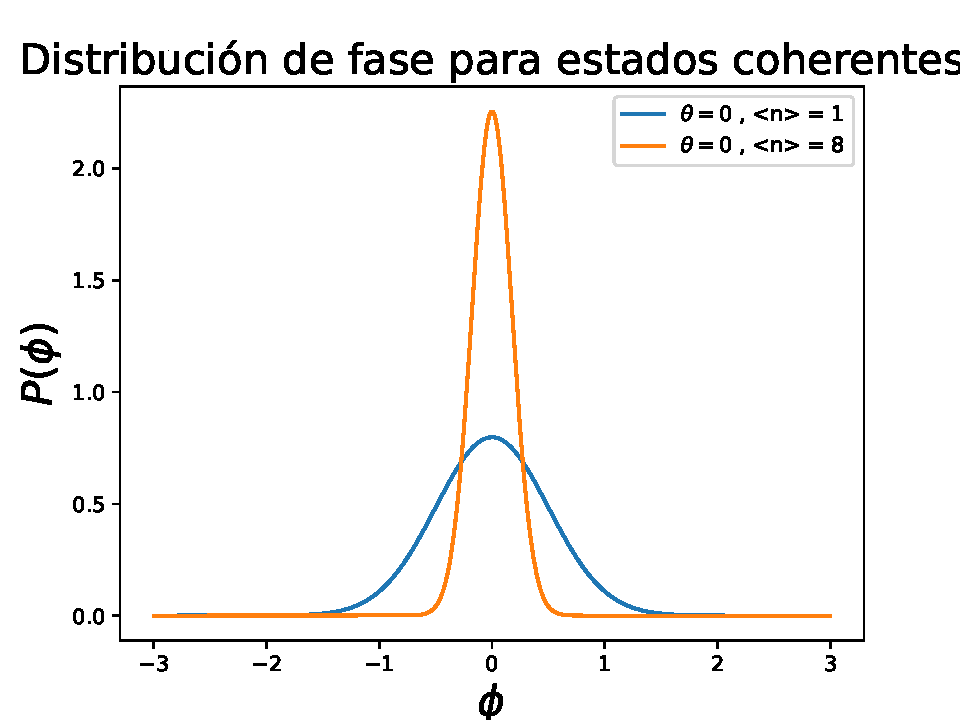
\includegraphics[width = 0.7\textwidth]{Capitulo 5/Figuras/DistribucionDeFaseCoherentes.pdf}
        \caption{Distribución de fase para los estados coherentes, en los cuales se ilustran dos estados centrados en el origen y con dos valores medios del número de cuantos de energía distintos.}
        \label{fig:DistriFaseCoherent}
    \end{figure}

    Podemos concluir que para los estados coherentes $\ket{\alpha}$ son estados cuánticos muy cercanos a estados clásicos porque:

    \begin{enumerate}
        \item El valor esperado del campo eléctrico tiene la forma de la expresión clásica.

        \item Las fluctuaciones en las variables del campo eléctrico son las mismas que para un vacío.

        \item Las fluctuaciones en la incertidumbre fraccional ($\frac{\Delta n}{\langle \hat{n} \rangle} = \frac{1}{\sqrt{\langle \hat{n}\rangle}}$) del número de cuantos de energía disminuyen a medida que aumenta el número promedio de estos.

        \item Los estados se vuelven bien localizados en fase a medida que aumenta el número promedio de fotones.
    \end{enumerate}


	\chapter{Coherencia cuántica y estadística de fotones}\label{chap:CoherenciaCuantica}
	\thispagestyle{empty}
	\vspace*{2cm}
	\begin{center}
		{\itshape\Huge Contar fotones de a uno resultó decir más sobre la luz que medir su intensidad. \par}
		\vspace{1cm}
		\epigraph{``Un haz de luz es coherente cuando todas sus funciones de correlación se factorizan''}{-- Roy J. Glauber}
	\end{center}
	\clearpage

	    En 1956 Robert Hanbury Brown y Richard Twiss publicaron un resultado que la comunidad óptica recibió con abierta incredulidad \citep{hanburybrown1956correlation}. Habían apuntado dos fotomultiplicadores a la misma fuente de luz térmica, habían multiplicado las dos corrientes y habían encontrado que las fluctuaciones estaban correlacionadas: cuando un detector registraba de más, el otro también. Poco después usaron el efecto para medir el diámetro angular de Sirio \citep{hanburybrown1956test}, con un instrumento que no medía amplitudes sino intensidades y que por tanto era inmune a la turbulencia atmosférica. Las objeciones fueron inmediatas, y no eran tontas: si la luz de una estrella consiste en fotones emitidos independientemente por átomos que ni siquiera se conocen entre sí, ¿por qué habrían de llegar en parejas a dos detectores separados? Edward Purcell contestó ese mismo año con un argumento de estadística de Bose y Einstein \citep{purcell1956question}, pero el asunto dejó claro que la teoría de la coherencia que teníamos, la de Wolf y la del capítulo segundo de estos apuntes, no bastaba: describía perfectamente las franjas de interferencia y no tenía nada que decir sobre las correlaciones de intensidad.

    Roy Glauber construyó la teoría que faltaba en tres artículos de 1963 \citep{glauber1963photon, glauber1963quantum}, y lo hizo partiendo de una pregunta que hasta entonces nadie se había tomado en serio: qué es exactamente lo que mide un fotodetector. La respuesta resultó fijar toda la estructura de la teoría, y de ella salieron las funciones de correlación de orden arbitrario, la definición precisa de lo que significa que un campo sea coherente, los estados coherentes que ya construimos en el capítulo anterior y el criterio que separa la luz que admite descripción clásica de la que no la admite. Este capítulo recorre esa construcción, muestra que la teoría clásica del capítulo segundo se recupera íntegra como el caso particular de primer orden, y termina en la polarización, que en este lenguaje es un caso de coherencia como cualquier otro.

\section{Qué mide un fotodetector}

    Un fotodetector funciona absorbiendo luz. El fotocátodo de un fotomultiplicador, la unión de un fotodiodo o el grano de una emulsión fotográfica registran un suceso cuando un electrón ligado es arrancado de su sitio, y la energía para arrancarlo la aporta el campo. Este hecho, que parece una trivialidad de ingeniería, tiene una consecuencia formal que Glauber fue el primero en explotar: el proceso de detección \textit{destruye} un cuanto del campo, de manera que la amplitud del proceso involucra al operador que destruye fotones y no al campo completo.

    Vamos a escribir esto con cuidado. El operador de campo eléctrico que construimos en el capítulo anterior se separa en dos partes, una que contiene solo operadores de aniquilación y otra que contiene solo operadores de creación,
    \begin{equation}\label{eq:CampoPartes}
        \hat{\mathbf{E}}(\mathbf{r},t) = \hat{\mathbf{E}}^{(+)}(\mathbf{r},t) + \hat{\mathbf{E}}^{(-)}(\mathbf{r},t),
        \qquad
        \hat{\mathbf{E}}^{(-)} = \left[\hat{\mathbf{E}}^{(+)}\right]^{\dagger},
    \end{equation}
    donde, para el campo libre desarrollado en modos,
    \begin{equation}\label{eq:CampoPositiva}
        \hat{\mathbf{E}}^{(+)}(\mathbf{r},t) = i\sum_{\mathbf{k},\lambda}\sqrt{\frac{\hbar\omega_{\mathbf{k}}}{2\epsilon_{0}V}}\;\hat{a}_{\mathbf{k},\lambda}\,\hat{\boldsymbol{\epsilon}}_{\mathbf{k},\lambda}\,e^{i(\mathbf{k}\cdot\mathbf{r}-\omega_{\mathbf{k}}t)} .
    \end{equation}
    La parte $\hat{\mathbf{E}}^{(+)}$ se llama de \textit{frecuencia positiva} porque su dependencia temporal es $e^{-i\omega t}$ con $\omega>0$, y es la que aniquila fotones; la parte $\hat{\mathbf{E}}^{(-)}$ los crea. En el lenguaje clásico del capítulo segundo estas dos partes eran la señal analítica y su conjugada, y la separación era una conveniencia matemática; aquí la separación es física, porque las dos partes hacen cosas distintas.

    Supongamos que el campo está en el estado $\ket{i}$ y que el detector, al absorber, lo deja en el estado $\ket{f}$. La amplitud de ese proceso es proporcional al elemento de matriz $\bra{f}\hat{\mathbf{E}}^{(+)}(\mathbf{r},t)\ket{i}$, y la probabilidad de que ocurra es el cuadrado de su módulo. Como en general no medimos en qué estado quedó el campo, la probabilidad total de que el detector se dispare es la suma sobre todos los estados finales posibles,
    \begin{equation}\label{eq:SumaFinales}
        w \propto \sum_{f}\left|\bra{f}\hat{\mathbf{E}}^{(+)}\ket{i}\right|^{2}
        = \sum_{f}\bra{i}\hat{\mathbf{E}}^{(-)}\ket{f}\bra{f}\hat{\mathbf{E}}^{(+)}\ket{i}
        = \bra{i}\hat{\mathbf{E}}^{(-)}\hat{\mathbf{E}}^{(+)}\ket{i},
    \end{equation}
    donde en el último paso se ha usado la relación de completitud $\sum_{f}\ket{f}\bra{f}=\hat{\mathbb{1}}$ del capítulo de los postulados. Si el campo no está en un estado puro sino descrito por una matriz densidad, el promedio se toma como siempre con una traza,
    \begin{equation}\label{eq:TasaDeteccion}
        w(\mathbf{r},t) \propto \mathrm{Tr}\left[\hat{\rho}\,\hat{\mathbf{E}}^{(-)}(\mathbf{r},t)\,\hat{\mathbf{E}}^{(+)}(\mathbf{r},t)\right] .
    \end{equation}

    El resultado \eqref{eq:TasaDeteccion} merece leerse con atención porque en él está contenida toda la teoría. Lo que un detector mide no es el valor medio de $\hat{\mathbf{E}}^{2}$, que sería lo que uno escribiría por analogía ingenua con la intensidad clásica, sino el valor medio del producto $\hat{\mathbf{E}}^{(-)}\hat{\mathbf{E}}^{(+)}$, en el cual todos los operadores de creación están a la izquierda de todos los de aniquilación. Ese ordenamiento se llama \textit{orden normal}, y la diferencia entre una cosa y la otra no es cosmética. Si evaluamos ambas expresiones en el vacío,
    \begin{equation}\label{eq:VacioDetector}
        \bra{0}\hat{\mathbf{E}}^{(-)}\hat{\mathbf{E}}^{(+)}\ket{0} = 0,
        \qquad\text{mientras que}\qquad
        \bra{0}\hat{\mathbf{E}}^{2}\ket{0} \neq 0,
    \end{equation}
    porque $\hat{\mathbf{E}}^{(+)}\ket{0}=0$ mientras que las fluctuaciones del vacío que calculamos en el capítulo anterior son distintas de cero. La primera igualdad dice que un detector colocado en la oscuridad no hace clic, que es lo que se observa; la segunda dice que el campo fluctúa igualmente. \textbf{El orden normal no es una convención de cálculo sino la huella matemática de que el detector absorbe}, y es la razón por la cual las fluctuaciones del vacío no saturan de ruido todos los fotodetectores del mundo.

\section{Las funciones de correlación de Glauber}

    La expresión \eqref{eq:TasaDeteccion} se refiere a un solo detector en un punto. Un experimento de interferencia compara el campo en dos puntos, y el experimento de Hanbury Brown y Twiss compara las intensidades en dos puntos, es decir, involucra cuatro factores de campo. La generalización es inmediata y es la definición de Glauber.

    Para abreviar, escribimos $x = (\mathbf{r},t)$ para un punto del espaciotiempo y omitimos los índices de polarización, que recuperaremos al final del capítulo.

    \begin{myDef}\label{def:GlauberN}
        La \textit{función de correlación de orden $n$} del campo, en el estado descrito por $\hat{\rho}$, es
        \begin{equation}\label{eq:GlauberN}
            G^{(n)}\left(x_{1},\ldots,x_{n};x_{n+1},\ldots,x_{2n}\right)
            = \mathrm{Tr}\left[\hat{\rho}\,\hat{E}^{(-)}(x_{1})\cdots\hat{E}^{(-)}(x_{n})\,\hat{E}^{(+)}(x_{n+1})\cdots\hat{E}^{(+)}(x_{2n})\right],
        \end{equation}
        con todos los operadores de creación a la izquierda y en orden normal.
    \end{myDef}

    Los dos primeros casos son los que usaremos sin descanso. El de orden uno,
    \begin{equation}\label{eq:G1}
        G^{(1)}(x_{1};x_{2}) = \mathrm{Tr}\left[\hat{\rho}\,\hat{E}^{(-)}(x_{1})\hat{E}^{(+)}(x_{2})\right],
    \end{equation}
    se reduce en la diagonal a la intensidad medida, $G^{(1)}(x;x) = I(x)$, y fuera de la diagonal es lo que gobierna la interferencia. El de orden dos,
    \begin{equation}\label{eq:G2}
        G^{(2)}(x_{1},x_{2};x_{2},x_{1}) = \mathrm{Tr}\left[\hat{\rho}\,\hat{E}^{(-)}(x_{1})\hat{E}^{(-)}(x_{2})\hat{E}^{(+)}(x_{2})\hat{E}^{(+)}(x_{1})\right],
    \end{equation}
    es la correlación entre las intensidades registradas en $x_{1}$ y en $x_{2}$, es decir, exactamente lo que mide un montaje de Hanbury Brown y Twiss. El orden de los argumentos en \eqref{eq:G2} no es caprichoso: los dos operadores de aniquilación actúan primero, en el orden en que los dos detectores absorben, y esa es la razón por la cual la expresión describe una detección conjunta y no un producto de dos detecciones independientes.

    Estas funciones tienen tres propiedades que se siguen directamente de su definición y que usaremos repetidamente. La primera es la simetría hermítica,
    \begin{equation}\label{eq:G1Hermitica}
        G^{(1)}(x_{1};x_{2}) = \left[G^{(1)}(x_{2};x_{1})\right]^{*},
    \end{equation}
    que se obtiene tomando el adjunto dentro de la traza y usando que $\hat{\rho}$ es autoadjunta. La segunda es la no negatividad de la diagonal,
    \begin{equation}\label{eq:G1Positiva}
        G^{(1)}(x;x) = \mathrm{Tr}\left[\hat{\rho}\,\hat{E}^{(-)}\hat{E}^{(+)}\right] \geq 0,
    \end{equation}
    porque es el valor medio de un operador de la forma $\hat{A}^{\dagger}\hat{A}$, cuyo valor esperado es la norma al cuadrado de $\hat{A}$ aplicado al estado. La tercera es una desigualdad de Cauchy y Schwarz,
    \begin{equation}\label{eq:CauchySchwarzG1}
        \left|G^{(1)}(x_{1};x_{2})\right|^{2} \leq G^{(1)}(x_{1};x_{1})\,G^{(1)}(x_{2};x_{2}),
    \end{equation}
    que es la misma que demostramos en el capítulo segundo para la función de coherencia clásica y que se obtiene aquí del mismo modo, tratando la traza como un producto interno entre los vectores $\hat{E}^{(+)}(x_{1})\ket{\psi}$ y $\hat{E}^{(+)}(x_{2})\ket{\psi}$.

    La desigualdad \eqref{eq:CauchySchwarzG1} permite normalizar la función de correlación de manera que su módulo quede acotado por la unidad. Definimos
    \begin{equation}\label{eq:g1}
        g^{(1)}(x_{1};x_{2}) = \frac{G^{(1)}(x_{1};x_{2})}{\sqrt{G^{(1)}(x_{1};x_{1})\,G^{(1)}(x_{2};x_{2})}},
        \qquad
        0 \leq \left|g^{(1)}\right| \leq 1,
    \end{equation}
    y análogamente, para la correlación de intensidades,
    \begin{equation}\label{eq:g2}
        g^{(2)}(x_{1},x_{2}) = \frac{G^{(2)}(x_{1},x_{2};x_{2},x_{1})}{G^{(1)}(x_{1};x_{1})\,G^{(1)}(x_{2};x_{2})} .
    \end{equation}
    El grado de coherencia de primer orden $g^{(1)}$ es el que hemos visto ya en el capítulo segundo, con otro nombre; el de segundo orden $g^{(2)}$ es nuevo y no tiene, como veremos, ninguna cota superior universal.

\section{Coherencia completa y los estados coherentes}

    Con las funciones de correlación en la mano podemos por fin decir qué significa que un campo sea coherente, cosa que en la teoría clásica se definía mediante la visibilidad de unas franjas y que aquí adquiere una formulación cerrada.

    \begin{myDef}\label{def:CoherenciaGlauber}
        Un campo es \textit{coherente en primer orden} si su función de correlación se factoriza,
        \begin{equation}\label{eq:FactorizaG1}
            G^{(1)}(x_{1};x_{2}) = \mathcal{E}^{*}(x_{1})\,\mathcal{E}(x_{2}),
        \end{equation}
        para alguna función compleja $\mathcal{E}$, y es \textit{completamente coherente} si todas sus funciones de correlación se factorizan de la misma manera,
        \begin{equation}\label{eq:FactorizaGN}
            G^{(n)}\left(x_{1},\ldots,x_{2n}\right) = \prod_{j=1}^{n}\mathcal{E}^{*}(x_{j})\prod_{j=n+1}^{2n}\mathcal{E}(x_{j}),
            \qquad \text{para todo } n .
        \end{equation}
    \end{myDef}

    La condición \eqref{eq:FactorizaG1} equivale a que $|g^{(1)}|=1$ en todo par de puntos, que es la definición clásica de coherencia completa en términos de visibilidad unidad. Lo nuevo es \eqref{eq:FactorizaGN}, porque un campo puede satisfacer la primera condición y fallar todas las demás, y de hecho eso es exactamente lo que le ocurre a la luz de una lámpara filtrada, que puede tener $|g^{(1)}|=1$ y sin embargo un $g^{(2)}$ igual a dos.

    ¿Existe algún estado del campo que satisfaga la condición a todos los órdenes? La respuesta es afirmativa y ya lo construimos en el capítulo anterior sin saber que cumplía esta propiedad. Un estado coherente $\ket{\alpha}$ es, por definición, estado propio del operador de aniquilación, y como $\hat{E}^{(+)}$ es una combinación lineal de operadores de aniquilación según \eqref{eq:CampoPositiva}, también es estado propio del campo de frecuencia positiva,
    \begin{equation}\label{eq:PropioCampo}
        \hat{E}^{(+)}(x)\ket{\alpha} = \mathcal{E}(x)\ket{\alpha},
        \qquad
        \mathcal{E}(x) = i\sum_{\mathbf{k},\lambda}\sqrt{\frac{\hbar\omega_{\mathbf{k}}}{2\epsilon_{0}V}}\;\alpha_{\mathbf{k},\lambda}\,e^{i(\mathbf{k}\cdot\mathbf{r}-\omega_{\mathbf{k}}t)},
    \end{equation}
    donde $\mathcal{E}(x)$ es un número complejo y no un operador. Tomando el adjunto, $\bra{\alpha}\hat{E}^{(-)}(x) = \mathcal{E}^{*}(x)\bra{\alpha}$. Al sustituir en la definición \eqref{eq:GlauberN}, cada operador puede actuar sobre el estado que tiene a su lado y sustituirse por su valor propio, de manera que la función de correlación de orden $n$ se convierte en un producto de números,
    \begin{equation}\label{eq:FactorizacionCoherente}
        G^{(n)} = \prod_{j=1}^{n}\mathcal{E}^{*}(x_{j})\prod_{j=n+1}^{2n}\mathcal{E}(x_{j})\;\underbrace{\braket{\alpha|\alpha}}_{=1},
    \end{equation}
    que es precisamente la condición \eqref{eq:FactorizaGN}. Los estados coherentes son, por lo tanto, completamente coherentes en el sentido de Glauber, y ahora sabemos en qué sentido preciso merecían el nombre que les dimos.

    De la factorización se sigue de inmediato el valor de los grados normalizados. Al dividir por las intensidades, los factores $\mathcal{E}$ se cancelan por pares y queda
    \begin{equation}\label{eq:gnCoherente}
        \left|g^{(1)}\right| = 1,
        \qquad
        g^{(2)} = 1,
        \qquad
        g^{(n)} = 1 \quad\text{para todo } n .
    \end{equation}
    Un haz en un estado coherente tiene correlaciones de intensidad que son exactamente las de sucesos independientes: saber que un detector hizo clic no cambia en nada la probabilidad de que el otro lo haga. Esa es la propiedad que distingue a la luz de un láser ideal y, como veremos, el valor $g^{(2)}=1$ es la frontera entre dos regiones del espacio de estados, una accesible a la descripción clásica y otra no.

\section{La recuperación de la teoría clásica}

    Antes de explorar lo que la teoría cuántica añade, es obligado verificar que no destruye lo que ya teníamos. El capítulo segundo construyó toda una teoría de la coherencia sobre un campo aleatorio clásico, y lo hizo con un aparato considerable de probabilidad; si la teoría de Glauber fuese incompatible con ella, el problema lo tendríamos aquí y no allá.

    El puente entre ambas descripciones es una representación del estado del campo que Glauber y Sudarshan introdujeron de manera independiente ese mismo año de 1963 \citep{sudarshan1963equivalence}. La idea consiste en escribir la matriz densidad como si fuese una mezcla estadística de estados coherentes,
    \begin{equation}\label{eq:RepresentacionP}
        \hat{\rho} = \int_{\mathbb{C}} P(\alpha)\,\ket{\alpha}\bra{\alpha}\;d^{2}\alpha,
        \qquad
        \int_{\mathbb{C}} P(\alpha)\,d^{2}\alpha = 1,
    \end{equation}
    donde $P(\alpha)$ es una función real llamada representación $P$ o distribución de Glauber y Sudarshan. La segunda condición es la traza unidad. Que semejante desarrollo exista para cualquier estado es un resultado nada obvio, y se debe a que los estados coherentes, pese a no ser ortogonales entre sí, forman un conjunto sobrecompleto.

    La utilidad de \eqref{eq:RepresentacionP} para nuestro propósito es que permite calcular cualquier correlación en orden normal de manera puramente clásica. Al sustituir la representación en la definición \eqref{eq:GlauberN} y usar que cada $\ket{\alpha}\bra{\alpha}$ es estado propio del campo, se obtiene
    \begin{equation}\label{eq:GnConP}
        G^{(n)} = \int_{\mathbb{C}} P(\alpha)\left[\prod_{j=1}^{n}\mathcal{E}^{*}_{\alpha}(x_{j})\prod_{j=n+1}^{2n}\mathcal{E}_{\alpha}(x_{j})\right]d^{2}\alpha,
    \end{equation}
    es decir, el promedio de un producto de amplitudes clásicas, pesado por la función $P$. Comparando \eqref{eq:GnConP} con las definiciones del capítulo segundo la conclusión es inmediata y merece enunciarse con precisión.

    \begin{myteo}\label{teo:RecuperacionWolf}
        Si la representación $P$ de un estado del campo es no negativa y suficientemente regular como para ser una densidad de probabilidad, entonces todas las funciones de correlación de Glauber coinciden con los promedios de conjunto de la teoría clásica de la coherencia, con $P(\alpha)$ jugando el papel de la medida de probabilidad sobre las realizaciones del campo aleatorio. En particular
        \begin{equation}\label{eq:G1esGamma}
            G^{(1)}\left(\mathbf{r}_{1},t_{1};\mathbf{r}_{2},t_{2}\right) = \left\langle \mathcal{E}^{*}(\mathbf{r}_{1},t_{1})\,\mathcal{E}(\mathbf{r}_{2},t_{2})\right\rangle = \Gamma\left(\mathbf{r}_{1},t_{1};\mathbf{r}_{2},t_{2}\right),
        \end{equation}
        donde $\Gamma$ es la función de coherencia mutua de Wolf.
    \end{myteo}

    La lectura de este teorema es que el capítulo segundo de estos apuntes sobrevive intacto. La función de coherencia mutua, el grado complejo de coherencia, el teorema de Wiener y Khinchin, la propagación de la coherencia y el teorema de Van Cittert y Zernike son enunciados sobre $G^{(1)}$, y $G^{(1)}$ es la misma cosa en las dos teorías siempre que la fuente admita una representación $P$ clásica, cosa que ocurre con todas las fuentes térmicas y con el láser ideal. La cuantización del campo no corrige ni una coma de la teoría clásica de la coherencia de primer orden, y esa es la razón por la cual la óptica funcionó durante siglo y medio sin necesidad de fotones.

    Lo que sí introduce la teoría cuántica es una frontera. La representación $P$ existe siempre, pero no siempre es una función bien comportada: hay estados para los cuales $P$ toma valores negativos, y estados para los cuales es tan singular que no se la puede escribir ni siquiera como una delta de Dirac, sino que exige derivadas de deltas. En esos casos \eqref{eq:GnConP} sigue siendo cierta como identidad formal, pero ya no puede interpretarse como el promedio de un campo aleatorio, porque una probabilidad negativa no describe ningún conjunto estadístico. Por eso se adopta el criterio siguiente, que es el que usaremos en el resto del capítulo: un estado del campo se llama \textit{clásico} cuando su representación $P$ es una densidad de probabilidad legítima, y \textit{no clásico} cuando no lo es.

\section{Estadística de fotones}

    Antes de calcular correlaciones de segundo orden vale la pena mirar la cantidad más simple que distingue unos estados de otros, que es la distribución del número de fotones. En un solo modo, la probabilidad de encontrar $n$ fotones es $p(n) = \bra{n}\hat{\rho}\ket{n}$, y las tres distribuciones que aparecen una y otra vez en el laboratorio son las siguientes.

    El estado de número $\ket{n_{0}}$ da, trivialmente, $p(n) = \delta_{n n_{0}}$, de manera que el número de fotones no fluctúa en absoluto y $\left(\Delta n\right)^{2} = 0$.

    El estado coherente $\ket{\alpha}$ da la distribución de Poisson que calculamos en el capítulo anterior,
    \begin{equation}\label{eq:PoissonCoh}
        p(n) = e^{-|\alpha|^{2}}\frac{|\alpha|^{2n}}{n!} = e^{-\bar{n}}\frac{\bar{n}^{n}}{n!},
        \qquad
        \bar{n} = |\alpha|^{2},
        \qquad
        \left(\Delta n\right)^{2} = \bar{n} .
    \end{equation}

    El estado térmico, cuya matriz densidad escribimos en el capítulo de los postulados, da una distribución geométrica. Sustituyendo el espectro del oscilador en los pesos de Boltzmann y usando la función de partición que allí calculamos,
    \begin{equation}\label{eq:BoseEinstein}
        p(n) = \frac{\bar{n}^{n}}{\left(1+\bar{n}\right)^{n+1}},
        \qquad
        \bar{n} = \frac{1}{e^{\hbar\omega/k_{B}T}-1},
    \end{equation}
    que es la distribución de Bose y Einstein. Su varianza se obtiene calculando $\langle n^{2}\rangle$ con la misma técnica de derivar la serie geométrica que usamos al deducir la ley de Planck, y el resultado es
    \begin{equation}\label{eq:VarianzaTermica}
        \left(\Delta n\right)^{2} = \bar{n} + \bar{n}^{2} .
    \end{equation}

    Las tres varianzas se comparan mejor si se las mide en unidades de la varianza de Poisson, y esa comparación es el contenido del parámetro que introdujo Mandel \citep{mandel1979sub},
    \begin{equation}\label{eq:MandelQ}
        Q = \frac{\left(\Delta n\right)^{2} - \bar{n}}{\bar{n}} .
    \end{equation}
    Para el estado coherente $Q=0$, para el térmico $Q = \bar{n} > 0$, y para el estado de número $Q = -1$, que es el valor mínimo posible. Las distribuciones con $Q>0$ se llaman \textit{super-Poissonianas} y las que tienen $Q<0$, \textit{sub-Poissonianas}.

    El signo de $Q$ resulta ser un criterio de no clasicidad, y la demostración es corta. Para un estado con representación $P$ positiva, el número medio y su cuadrado se calculan promediando sobre $P$, y un cálculo directo da
    \begin{equation}\label{eq:VarianzaConP}
        \left(\Delta n\right)^{2} = \bar{n} + \int_{\mathbb{C}} P(\alpha)\left(|\alpha|^{2} - \bar{n}\right)^{2}d^{2}\alpha .
    \end{equation}
    El primer término es la varianza de Poisson y el segundo es la varianza de $|\alpha|^{2}$ respecto de la distribución $P$. Si $P$ es una densidad de probabilidad legítima ese segundo término es no negativo, por ser la integral de un cuadrado con un peso positivo, y por lo tanto
    \begin{equation}\label{eq:CotaClasicaQ}
        \left(\Delta n\right)^{2} \geq \bar{n},
        \qquad\text{es decir}\qquad
        Q \geq 0 .
    \end{equation}
    Ninguna fuente descriptible como un campo aleatorio clásico puede producir fluctuaciones de número menores que las de Poisson. Observar $Q<0$ es, por tanto, observar algo que ninguna teoría ondulatoria clásica puede reproducir, y la primera medida de luz sub-Poissoniana fue precisamente el experimento de fluorescencia de resonancia de Kimble, Dagenais y Mandel que mencionamos en la historia del capítulo quinto \citep{kimble1977photon}.

\section{Agrupamiento, antiagrupamiento y el experimento de Hanbury Brown y Twiss}

    Pasemos ahora a la correlación de segundo orden, que es donde la teoría cuántica dice algo genuinamente nuevo. Para un solo modo, y con los dos detectores midiendo al mismo tiempo, la definición \eqref{eq:g2} se reduce a
    \begin{equation}\label{eq:g2UnModo}
        g^{(2)}(0) = \frac{\left\langle \hat{a}^{\dagger}\hat{a}^{\dagger}\hat{a}\hat{a}\right\rangle}{\left\langle \hat{a}^{\dagger}\hat{a}\right\rangle^{2}},
    \end{equation}
    y el numerador se expresa en términos del operador número usando la relación de conmutación. Escribiendo $\hat{a}^{\dagger}\hat{a}^{\dagger}\hat{a}\hat{a} = \hat{a}^{\dagger}\left(\hat{a}\hat{a}^{\dagger}-\textcolor{blue}{1}\right)\hat{a} = \hat{n}^{2}-\hat{n}$, donde el uno en azul es el conmutador que se ha insertado al intercambiar los dos operadores centrales, queda
    \begin{equation}\label{eq:g2Numero}
        g^{(2)}(0) = \frac{\left\langle \hat{n}^{2}\right\rangle - \left\langle \hat{n}\right\rangle}{\left\langle \hat{n}\right\rangle^{2}}
        = 1 + \frac{\left(\Delta n\right)^{2}-\bar{n}}{\bar{n}^{2}}
        = 1 + \frac{Q}{\bar{n}},
    \end{equation}
    donde en el segundo paso se ha sumado y restado $\bar{n}^{2}$ en el numerador para hacer aparecer la varianza. La relación \eqref{eq:g2Numero} conecta las dos medidas de no clasicidad que hemos introducido y muestra que son la misma cosa vista de dos maneras.

    Los tres estados de referencia dan entonces
    \begin{equation}\label{eq:g2Tres}
        g^{(2)}_{\text{coherente}}(0) = 1,
        \qquad
        g^{(2)}_{\text{térmico}}(0) = 2,
        \qquad
        g^{(2)}_{\ket{n}}(0) = 1 - \frac{1}{n},
    \end{equation}
    resultados que se obtienen sustituyendo en \eqref{eq:g2Numero} los valores de $Q$ y $\bar{n}$ de la sección anterior. El caso del estado de un solo fotón es el más elocuente: con $n=1$ se obtiene $g^{(2)}(0)=0$ exactamente, porque un único cuanto no puede ser absorbido por dos detectores. Este es, en el lenguaje que ahora tenemos, el contenido del experimento de Grangier, Roger y Aspect que discutimos en el capítulo quinto, cuyo parámetro de anticorrelación $\alpha$ no es otra cosa que $g^{(2)}(0)$ medido con un fotón anunciado.

    La cota clásica para $g^{(2)}$ se obtiene igual que la de $Q$. Para un estado con $P$ positiva,
    \begin{equation}\label{eq:g2Clasico}
        g^{(2)}(0) = \frac{\displaystyle\int P(\alpha)\,|\alpha|^{4}\,d^{2}\alpha}{\left[\displaystyle\int P(\alpha)\,|\alpha|^{2}\,d^{2}\alpha\right]^{2}}
        = \frac{\left\langle I^{2}\right\rangle}{\left\langle I\right\rangle^{2}} \geq 1,
    \end{equation}
    donde la desigualdad final es de nuevo la no negatividad de la varianza de una cantidad real. Todo campo clásico tiene $g^{(2)}(0)\geq 1$, y los valores menores que uno son inaccesibles a cualquier descripción ondulatoria. Un cálculo del mismo tipo, aplicado a dos instantes distintos, da además la condición clásica $g^{(2)}(0) \geq g^{(2)}(\tau)$, es decir, que la correlación nunca puede crecer al separar los detectores en el tiempo.

    Estas desigualdades dan nombre a los tres comportamientos posibles. Cuando $g^{(2)}(0) > 1$ los fotones tienden a llegar en grupos y se habla de \textit{agrupamiento}; cuando $g^{(2)}(0) = 1$ llegan de manera completamente independiente, como los sucesos de un proceso de Poisson; y cuando $g^{(2)}(0) < 1$ tienden a separarse unos de otros y se habla de \textit{antiagrupamiento}. Solo el tercero carece de análogo clásico.

    El resultado de Hanbury Brown y Twiss queda ahora explicado. La luz térmica tiene $g^{(2)}(0)=2$, es decir, la probabilidad de detectar dos fotones simultáneamente en dos detectores es el doble de la que tendrían sucesos independientes, y por eso las corrientes de los dos fotomultiplicadores fluctúan al unísono. El origen físico del factor dos es la estadística de Bose y Einstein, como Purcell argumentó: los fotones son bosones y tienden a ocupar el mismo modo, de manera que las fluctuaciones de intensidad de una fuente térmica son mayores que las de una fuente que emitiese cuantos independientes. En términos de la representación $P$, la luz térmica es una gaussiana ancha en el plano complejo, y la anchura de esa gaussiana es exactamente el exceso de fluctuación que produce el agrupamiento.

    La objeción que se le hizo al experimento en 1956 tenía, en el fondo, una respuesta sencilla que vale la pena enunciar porque ilumina la diferencia entre las dos teorías. Los átomos de la estrella emiten independientemente, es cierto, pero lo que llega al detector no es una colección de fotones etiquetados por su átomo de origen sino un campo cuyas amplitudes se superponen, y la intensidad resultante fluctúa porque las fases relativas de esas contribuciones cambian al azar. Esas fluctuaciones de intensidad son las que se correlacionan en los dos detectores, y existen ya en la descripción clásica; lo que la descripción cuántica añade no es el agrupamiento térmico sino la posibilidad de lo contrario, el antiagrupamiento, que fue medido por primera vez veintiún años más tarde \citep{kimble1977photon}.

    Con esto se completa la imagen que veníamos construyendo desde el capítulo segundo. La coherencia de primer orden mide la capacidad del campo de producir franjas y es idéntica en las dos teorías; la de segundo orden mide cómo llegan los fotones unos respecto de otros, y es allí donde aparecen estados que ninguna función de probabilidad positiva puede describir. Un haz térmico filtrado puede tener $|g^{(1)}|$ tan próximo a uno como se quiera, es decir, ser tan coherente como un láser a primer orden, y sin embargo delatarse de inmediato en $g^{(2)}$. \textbf{La visibilidad de las franjas no distingue la luz clásica de la cuántica; la estadística de las llegadas sí.}

\section{Coherencia y polarización}

    Queda por conectar todo esto con la polarización, que hasta ahora hemos tratado aparte y que en este lenguaje resulta ser un caso particular de coherencia. La observación de partida ya apareció en el capítulo segundo: la polarización es la coherencia entre las dos componentes transversales del campo en un mismo punto, del mismo modo que la coherencia espacial es la que hay entre dos puntos distintos.

    Recuperemos entonces los índices de polarización que habíamos omitido. Para un solo punto del espaciotiempo y las dos componentes transversales $i,j \in \{x,y\}$, la función de correlación de primer orden es una matriz de dos por dos,
    \begin{equation}\label{eq:MatrizCoherenciaCuantica}
        J_{ij} = \mathrm{Tr}\left[\hat{\rho}\,\hat{E}^{(-)}_{i}(x)\,\hat{E}^{(+)}_{j}(x)\right],
    \end{equation}
    que es el análogo cuántico exacto de la matriz de coherencia de Wolf. Sus propiedades se siguen de las que ya demostramos para $G^{(1)}$: es hermítica por \eqref{eq:G1Hermitica}, sus elementos diagonales son no negativos por \eqref{eq:G1Positiva}, y su determinante es no negativo por la desigualdad de Cauchy y Schwarz \eqref{eq:CauchySchwarzG1}. Es, por tanto, una matriz semidefinida positiva, igual que en la teoría clásica.

    Los parámetros de Stokes son las cuatro combinaciones lineales independientes de sus elementos,
    \begin{equation}\label{eq:StokesDesdeJ}
        S_{0} = J_{xx}+J_{yy},
        \qquad
        S_{1} = J_{xy}+J_{yx},
        \qquad
        S_{2} = i\left(J_{yx}-J_{xy}\right),
        \qquad
        S_{3} = J_{xx}-J_{yy},
    \end{equation}
    escritas con el mismo ordenamiento que se usa en el capítulo dedicado a la fase cuántica, y el grado de polarización se obtiene de la misma expresión que en la teoría clásica,
    \begin{equation}\label{eq:GradoPolarizacion}
        \mathcal{P} = \frac{\sqrt{S_{1}^{2}+S_{2}^{2}+S_{3}^{2}}}{S_{0}} = \sqrt{1 - \frac{4\det J}{\left(\mathrm{tr}\,J\right)^{2}}},
    \end{equation}
    donde la segunda forma se obtiene desarrollando el determinante y la traza en términos de los elementos de la matriz. La luz completamente polarizada corresponde a $\det J = 0$, es decir, a una matriz de rango uno, que es la condición de factorización \eqref{eq:FactorizaG1} aplicada a los índices de polarización en lugar de a los puntos del espaciotiempo. La luz no polarizada corresponde a $J$ proporcional a la identidad.

    Esta coincidencia con la teoría clásica no es casual y es, otra vez, el teorema \ref{teo:RecuperacionWolf} en acción: las cuatro cantidades \eqref{eq:StokesDesdeJ} son correlaciones de primer orden, y las correlaciones de primer orden son idénticas en las dos teorías. De hecho, en el capítulo dedicado a la fase cuántica se definen los operadores de Stokes $\hat{S}_{i}$ en términos de los operadores de creación y aniquilación de los dos modos de polarización, y se comprueba que sus valores medios en un estado coherente bimodal reproducen exactamente los parámetros clásicos \eqref{eq:StokesDesdeJ}. Lo que allí se calcula es esto mismo visto desde el lado de los operadores.

    La diferencia entre ambas teorías aparece, como cabía esperar a estas alturas, en el segundo orden. Los operadores de Stokes no conmutan entre sí, de manera que sus fluctuaciones están sujetas a relaciones de indeterminación y no pueden anularse simultáneamente; existe un ruido de polarización irreducible que la teoría clásica desconoce. Y existen estados cuyos cuatro parámetros de Stokes medios se anulan, de modo que la teoría clásica los declararía no polarizados, pero cuyas fluctuaciones de polarización son marcadamente distintas de las de la luz térmica no polarizada. Esos estados, a los que a veces se llama de polarización escondida, son no clásicos en el mismo sentido preciso en que lo era la luz con $g^{(2)}(0)<1$: su representación $P$ no es una densidad de probabilidad.

    El cuadro que resulta de todo el capítulo puede resumirse así. La teoría de Glauber no sustituye a la de Wolf sino que la contiene: todo lo que el capítulo segundo dice sobre franjas, visibilidad, anchura espectral, propagación de la coherencia y polarización sigue siendo cierto palabra por palabra, porque son enunciados sobre $G^{(1)}$. Lo que la teoría cuántica añade es un piso inferior, el de las correlaciones de orden dos y superiores, en el cual viven fenómenos que ninguna distribución de probabilidad sobre campos clásicos puede reproducir, y es allí donde la óptica cuántica deja de ser una manera elegante de reescribir la óptica y empieza a describir cosas que la óptica no podía describir.


	\chapter{La fase cuántica}\label{chap:FaseCuantica}
	\thispagestyle{empty}
	\vspace*{2cm}
	\begin{center}
		{\itshape\Huge De todas las variables del campo, la fase es la que se resiste a convertirse en operador. \par}
		\vspace{1cm}
		\epigraph{``La fase de un campo cuántico es una cantidad tan fundamental como difícil de definir''}{-- Peter L. Knight}
	\end{center}
	\clearpage

	    Este problema fue abordado en un inicio por Paul Dirac en los primeros años de la mecánica cuántica. Sin embargo, su propuesta de un operador de fase cuántica se demostró que poseía bastantes inconsistencias matemáticas. Posterior a Dirac varios científicos abordaron el problema de diferentes maneras en esta sección vamos a abordar el formalismo de Dirac y Susskind-Glogower y nuestra solución al problema mediante el formalismo de Fourier Fraccionario.
    
\section{La fase de Dirac}

        Para entender la propuesta de Dirac vamos a aproximarnos desde un régimen clásico, planteando campos y a partir definir operadores. Consideremos la cavidad mostrada en la figura \ref{fig:cavidad}. Clásicamente el vector de campo eléctrico $\vec{E}(\vec{r},t)$ puede ser expandido como una superposición de ondas planas cada una caracterizada por un vector de onda $\vec{k}$ y vector de polarización $\hat{e}_{k}$. Por conveniencia vamos a limitar el desarrollo a un campo linealmente polarizado con una sola frecuencia. Esta suposición permite tratar el campo eléctrico mediante una descomposición del tipo

        \begin{equation}
            \vec{E}(\vec{r},t) = \left( \frac{\hbar \omega}{2\epsilon_0 L^3} \right)^{1/2} \sum_k \left[a_k e^{i(\vec{k}\cdot \vec{r} - \omega t)} + a_k^* e^{-i( \vec{k}\cdot \vec{r} - \omega t )}  \right],
        \end{equation}

        donde $\omega$ es la frecuencia angular y $\epsilon_0$ es la permitividad eléctrica en el vacío. El conjunto de vectores de onda $\{\vec{k_i}\}$ en la expansión está determinada por las condiciones de fronteras de la onda electromagnética dentro de la cavidad \ref{fig:cavidad}. Si acotamos las condiciones a un campo monomodal, es decir, tenemos un solo vector de onda $\vec{k}=\vec{k}_0$ y se pierde la dependencia de $\vec{k}$ de $a_k$, entonces 

        \begin{equation}
            \vec{E}(\vec{r},t) = \left( \frac{\hbar \omega}{2\epsilon_0 L^3} \right)^{1/2} \left[ ae^{i( \vec{k}\cdot\vec{r} - \omega t )} + a^* e^{-i ( \vec{k}\cdot \vec{r} - \omega t )} \right].
        \end{equation}

        El uso de $a$ es una conveniencia, puesto que no representa nada más que la amplitud adimensional del campo eléctrico, medida en unidades del campo por cuanto $\left(\hbar\omega/2\epsilon_{0}L^{3}\right)^{1/2}$, y su utilidad radica en el papel que juega a la hora de definir los operadores de creación y destrucción. Siguiendo este desarrollo, como $a$ es un número complejo, este se puede expresar en su forma polar como $a = re^{i\phi}$, por lo que la expresión del campo eléctrico se reduce a 

        \begin{equation}
            \vec{E}(\vec{r},t) = \vec{E}_0 \cos\left( \vec{k}_0\cdot \vec{r} - \omega t + \phi \right),\quad \text{donde} \quad \vec{E}_0 = \left( \frac{2\hbar \omega}{\epsilon_0 L^3} \right)^{1/2}r \hat{e},
        \end{equation}
        la cual es la descomposición clásica de amplitud $E_0$ y fase $\phi$.

        Tomando los campos como operadores y definiendo los operadores de creación y aniquilación que satisfacen la relación de conmutación $\left[ \hat{a}, \hat{a}^\dagger \right] = 1$. Debido a que las cantidades en mecánica cuántica son operadores y no números complejos, la descomposición en amplitud y fase no es viable, de hecho, se convierte en un problema realmente difícil. 

        Para abordar el formalismo de Dirac, vamos a partir de la composición polar de las amplitudes clásicas $a = Re^{i\phi}$ en donde se puede despejar al exponencial de fase como $e^{i\phi} = a/R$. De manera análoga, Dirac planteó una descomposición polar para el exponencial de fase como sigue

        \begin{equation}
            e^{i\hat{\phi}} = \hat{a} \hat{R}^{-1},
        \end{equation}
        asumiendo que $e^{i\phi}$ es un exponencial de fase, donde asumiremos que el operador de fase $\hat{\phi}$ es hermítico, y que la amplitud $\hat{R}$ es también un operador hermítico, por ende tenemos que el operador de creación se escribe como

        \begin{equation}
            \hat{a}^{\dagger} = \left( e^{i\hat{\phi}} \hat{R} \right)^\dagger = \hat{R}e^{-i\hat{\phi}},
        \end{equation}
        con esto en cuenta, podemos encontrar la relación entre $\hat{R}$ y el operador número $\hat{N}$ como sigue

        \begin{equation}
            \hat{a}^\dagger\hat{a} = \hat{N} = \hat{R} e^{-i\hat{\phi}}e^{i\hat{\phi}}\hat{R} = \hat{R}^2 \rightarrow \hat{R} = \hat{N}^{1/2}.
        \end{equation}
        Con esto en cuenta el operador exponencial de fase de Dirac se define como 

        \begin{equation}\label{eq:ExpDirac}
            e^{i\hat{\phi}} = \hat{a}\hat{N}^{-1/2}.
        \end{equation}

        Para darnos cuenta de los problemas de este operador de exponencial de fase \ref{eq:ExpDirac} vamos a encontrar las relaciones de conmutación fundamentales relacionados a este operador. Primero la relación de conmutación entre el exponencial de fase y el operador número

        \begin{align}
            & \left[ e^{i\hat{\phi}}, \hat{N} \right] = e^{i\hat{\phi}}\hat{N} - \hat{N}e^{i\hat{\phi}} = e^{i\hat{\phi}}\hat{N} - \hat{a}^\dagger\hat{a} \hat{a} \hat{N}^{-1/2},\\
            & \left[ e^{i\hat{\phi}}, \hat{N} \right] = e^{i\hat{\phi}}\hat{N} - \left( \hat{a}\hat{a}^\dagger -1 \right)\hat{a}\hat{N}^{-1/2} = e^{i\hat{\phi}}\hat{N}- \hat{a}\hat{N}\hat{N}^{-1/2} + \hat{a}\hat{N}^{-1/2},\\
            & \left[ e^{i\hat{\phi}}, \hat{N} \right] = e^{i\hat{\phi}}\hat{N} - e^{i\hat{\phi}}\hat{N} + e^{i\hat{\phi}},\\
            & \left[ e^{i\hat{\phi}}, \hat{N} \right] = e^{i\hat{\phi}},
        \end{align}
        usualmente conocido como el criterio de Lerner. A partir de la relación de conmutación  $\left[ e^{i\hat{\phi}}, \hat{N} \right] = e^{i\hat{\phi}}$ podemos obtener la relación de conmmutación entre $\hat{N},\hat{\phi}$, para ello, usamos el siguiente teorema; dados $\hat{A},\hat{B}$ dos operadores, y $f$ algún funcional diferenciable, se tiene que

        \begin{equation}
            \left[\hat{A},f\left( \hat{B} \right)\right] = \frac{\partial f}{\partial \hat{B}} [\hat{A},\hat{B}].
        \end{equation}
        Si tomamos a $\hat{A}=\hat{N}$ y a $\hat{B}=e^{i\hat{\phi}}$ tendremos el siguiente resultado

        \begin{align}\label{eq:ComNPhi}
            & \left[ \hat{N}, e^{i\hat{\phi}} \right] = ie^{i\hat{\phi}}\left[\hat{N},\hat{\phi} \right] = -e^{i\hat{\phi}},\\
            & \left[\hat{N}, \hat{\phi}\right] = i.
        \end{align}
        Esta relación de conmutación lo que muestra que el operador número $\hat{N}$ y el operador de fase $\hat{\phi}$ son pares canónicamente  conjugados, (cabe recalcar que no aparece $\hbar$ debido a que el operador número y el operador de fase son adimensionales). Esta ecuación, inmediatamente nos lleva a una relación de incertidumbre la cual es frecuentemente vista en discusiones fenomenológicas en las fluctuaciones del número y fase del campo óptico

        \begin{align}
            & \Delta \hat{N}\, \Delta \hat{\phi} \geq \frac{1}{2}\left| \left\langle [\hat{N},\hat{\phi}]\right\rangle \right| = \frac{1}{2}.
        \end{align}

        Hasta el momento todo parece correcto y bien direccionado, sin embargo, en todo el desarrollo previo surgen varios errores. Por ejemplo, si tomamos los elementos de matriz del conmutador \ref{eq:ComNPhi} en la base de los estados número $\ket{n},\ket{n'}$, donde $\hat{N}\ket{n'}=N'\ket{n'}$ tendremos

        \begin{align}
            & \bra{n}\left( \hat{N}\hat{\phi} - \hat{\phi}\hat{N} \right) \ket{n'} = i \braket{n|n'} ,\\
            & (n-n')\bra{n}\hat{\phi}\ket{n'} = i \delta_{nn'}.
        \end{align}
        Para $n=n'$ se llega a una singularidad, a una ecuación $0=i$. Susskind y Glogower también demostraron que el exponencial de fase definido por Dirac no es un operador unitario, y la raíz del problema está en que $\hat{N}^{-1/2}$ no está definido sobre el estado de vacío, pues $\hat{N}\ket{0} = 0$. Adoptando la convención natural de que $\hat{N}^{-1/2}\ket{0}=0$, los dos productos resultan distintos,
        \begin{align}
            & e^{i\hat{\phi}}e^{-i\hat{\phi}} = \hat{a}\hat{N}^{-1/2} \hat{N}^{-1/2}\hat{a}^\dagger = \hat{a}\hat{N}^{-1}\hat{a}^\dagger = \mathbb{I},\\
            & e^{-i\hat{\phi}}e^{i\hat{\phi}} = \hat{N}^{-1/2}\hat{a}^\dagger\hat{a}\hat{N}^{-1/2} = \hat{N}^{-1/2}\hat{N}\hat{N}^{-1/2}= \mathbb{I} - \ket{0}\bra{0},
        \end{align}
        donde el primero sí reproduce la identidad, porque $\hat{a}^{\dagger}$ saca al estado del vacío antes de que actúe $\hat{N}^{-1}$, mientras que el segundo falla precisamente sobre $\ket{0}$. \textbf{La no unitariedad del exponencial de fase de Dirac se concentra por completo en el estado de vacío}, y esa es la razón por la cual no existe un operador hermítico $\hat{\phi}$ del cual $e^{i\hat{\phi}}$ sea la exponencial.

        \begin{figure}[htbp]
            \centering
            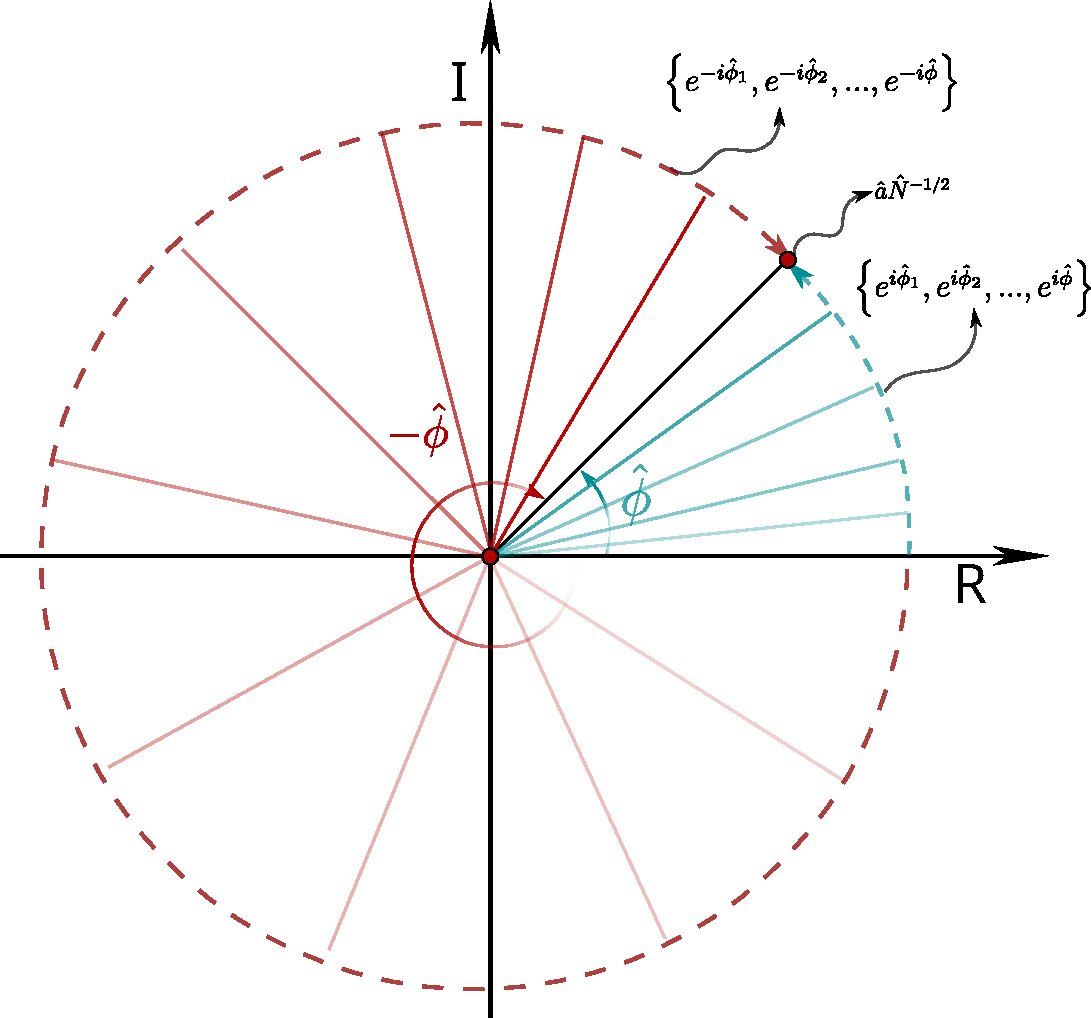
\includegraphics[width=0.7\linewidth]{Capitulo 7/Figuras/FaseDirac.pdf}
            \caption{Representación esquemática sobre el plano complejo $\mathbb{C}^2$ en el cual se ve el efecto del exponencial de fase $e^{i\hat{\phi}}$ y de su adjunto
            $e^{-i\hat{\phi}}$.}
            \label{fig:FaseDirac}
        \end{figure}
        
        Antes de seguir abordando los problemas de la fase de Dirac demos algo de sentido geométrico a la no unitaridad del operador exponencial de fase. En la figura \ref{fig:FaseDirac} se representa esquemáticamente distintas rotaciones sobre el plano complejo $\mathbb{C}^2$ que representa el exponencial de fase $e^{i\hat{\phi}}$ de color azul, en donde se sigue la convención de rotaciones en sentido antihorario mientras que de color rojo se representan las rotaciones relacionado al operador $e^{-i\hat{\phi}}$. Cuando trabajamos sobre el cuerpo de los números complejos se tiene que todo complejo $z \in \mathbb{C}$ tiene una representación polar en donde el exponencial de fase satisface que es unitario pero, esta propiedad viene heredada de la naturaleza conmutativa de $\mathbb{C}$ acá hemos demostrado \ref{eq:ComNPhi} que no hay conmutación, por ende, es natural que el exponencial de fase propuesto por Dirac no sea unitario, ambos representan procesos físicos distintos como se trata de ilustrar en la figura \ref{fig:FaseDirac}.

        Los problemas del formalismo de Dirac se pueden identificar de dos fuentes. La primera es que el espectro de $n$ no se extiende a valores negativos, sino que solo por los enteros no negativos desde $0$ hasta $+\infty$. Para entender un poco esto vamos a ver el desarrollo de Barnett y Pegg e introducir estados número negativos, tal que podemos escribir la siguiente expresión

        \begin{equation}
            e^{i\hat{\phi}} = \sum_{n=-\infty}^{\infty} \ket{n}\bra{n+1},
        \end{equation}
        y es fácil ver que el adjunto conjugado es el operador
        \begin{equation}
            e^{-i\hat{\phi}} = \sum_{n=-\infty}^{\infty}\ket{n+1}\bra{n},
        \end{equation}
        en donde podemos verificar que este exponencial de fase es unitario

        \begin{align}\label{eq:Pegg}
            &e^{i\hat{\phi}}e^{-i\hat{\phi}} = \sum_{n,n'=-\infty}^{\infty} \ket{n}\braket{n+1|n'+1}\bra{n'} = \sum_{n,n'=-\infty}^{\infty}\ket{n}\delta_{nn'}\bra{n'} = \sum_{n=-\infty}^\infty\ket{n}\bra{n}= \mathbb{I},\\
            & e^{-i\hat{\phi}}e^{i\hat{\phi}} = \sum_{n,n'=-\infty}^{\infty}\ket{n+1}\braket{n|n'}\bra{n'+1} = \sum_{n,n'=-\infty}^{\infty}\ket{n+1}\delta_{nn'}\bra{n+1} = \sum_{n=-\infty}^{\infty}\ket{n+1}\bra{n+1}= \mathbb{I}
        \end{align}

        Vale la pena notar que los estados número negativos son solamente una herramienta matemática que permite definir un operador unitario pero no tienen sentido físico. Así como Barnett y Pegg mencionaron "... la deducción de los estados propios del oscilador armónico se requiere un estado base que es aniquilado por el operador de aniquilación tal que el espectro de energía es acotado desde abajo... Estados de energía negativa no están excluidos pero ellos deben desprenderse de los estados de base de energía positiva que son aniquilados por el operador de aniquilación... Estados que contienen un número negativo de fotones son inaccesibles a un sistema físico, por lo tanto, su mera existencia en el formalismo no predice ningún fenómeno nuevo en la electrodinámica cuántica".

        Debido a que $e^{i\hat{\phi}}$ es un operador unitario este define un operador hermítico $\hat{\phi}$. De la ecuación \ref{eq:Pegg} se puede deducir un conmutador como el de la regla de Lerner

        \begin{equation}
            \left[ e^{i\hat{\phi}},\hat{N} \right] = e^{i\hat{\phi}},
        \end{equation}
        que de manera análoga nos lleva a la conmutación canónica entre $\hat{N},\hat{\phi}$ y se repite el problema de tener una ecuación singular del tipo $0=i$ como pasó con el exponencial de Dirac.

        La fuente de problemas restante se debe a que $\hat{\phi}$ es un operador de ángulo. Esto se puede apreciar mejor al comparar este tratamiento de fase y número con algún problema análogo, como el momento angular y su variable conjugada. En esta analogía, el operador de momento angular $\hat{L}$, entendido como cualquiera de sus componentes, hace el papel del operador número. Sin embargo, como se vio, la introducción de estados número negativos es una herramienta matemática más no física, entonces los valores propios de $\hat{L}$ pertenecientes al estado propio $\ket{m}$ realmente generan el rango de enteros que van desde $-\infty$ hasta $\infty$. Vamos a asumir que $\hat{L}$ y su ángulo canónicamente conjugado $\hat{\chi}$ satisfacen la relación de conmutación

        \begin{equation}
            \left[ \hat{L},\hat{\chi} \right] = i.
        \end{equation}

        En la base de $\chi$ los operadores toman la forma $\hat{\chi}\to \chi$ y $\hat{L}\to -i\frac{\partial}{\partial\chi}$. Las funciones propias de $\hat{L}$, $\braket{\chi|m}$, son simplemente proporcionales a $e^{im\chi}$. $m$ se convierte en un valor entero después de imponer la condición de que $\chi \to \chi + 2\pi$. En este orden de ideas, las funciones propias base son periódicas, con periodos de $2\pi$. Sin embargo, debemos restringir el rango de $\chi$, puesto que este cubre a todo $\mathbb{R}.$

        \begin{figure}[htbp]
            \centering
            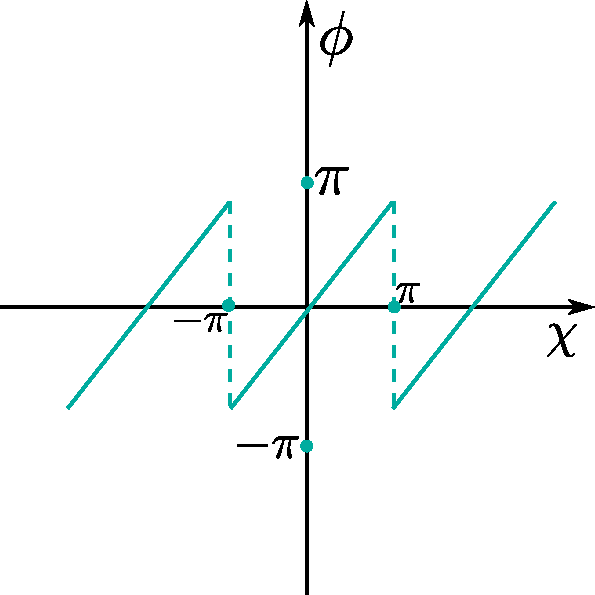
\includegraphics[width=0.5\linewidth]{Capitulo 7/Figuras/chivsphi.pdf}
            \caption{Relación entre el operador de ángulo restringido $\hat{\phi}$ con $-\pi < \hat{\phi} \leq \pi$ y el operador de ángulo $\hat{\chi}$.}
            \label{fig:chivsphi}
        \end{figure}

        Un resultado de esto es que $\hat{\chi}$ opera impropiamente sobre el espacio de las funciones propias, a pesar de que $\braket{\chi|m}$ es periódico en $\chi$, $\hat{\chi}\braket{\chi|m}$ no lo es. Una forma de salir de este problema es introduciendo un ángulo $\phi$ relacionado con $\chi$, el cual es periódico. Si escogemos el intervalo de periodicidad de manera arbitraria, como por ejemplo, $-\pi$ a $\pi$, entonces la relación entre $\hat{\chi}$ y $\hat{\phi}$ se muestra en la figura \ref{fig:chivsphi}.

        Volviendo al conmutador, recordando que el operador $\hat{L}$ es una derivada parcial y recordando las discontinuidades que hay en la relación de $\phi vs \chi$ esta da lugar a una función delta de Dirac, por ende tenemos

        \begin{equation}\label{eq:phires}
            \left[ \hat{L},\hat{\phi} \right] = i - 2\pi i \delta(\phi-\pi), \quad -\pi < \phi \leq \pi. 
        \end{equation}

        El mismo argumento aplica a la relación de conmutación $[\hat{N},\hat{\phi}]$ ya que esta es isomorfa a la conmutación $[\hat{L},\hat{\phi}]$ en donde el espectro de $n$ se extiende a valores negativos. Con esta relación de conmutación \ref{eq:phires}, si calculamos los elementos de matiz en la base de los estados número tendremos ahora

        \begin{equation}
            \bra{n} \left( \hat{N}\hat{\phi} - \hat{\phi}\hat{N} \right) \ket{n'} = i \left[ 1 - 2\pi \bra{n}\delta(\phi-\pi) \ket{n'} \right].
        \end{equation}
        Recordemos que $\braket{\phi|n}\propto e^{in\phi}$ en esta representación, entonces tenemos

        \begin{equation}
            (n-n')\bra{n}\hat{\phi}\ket{n'} = i \left[ 1 - e^{i(n'-n)\pi} \right],
        \end{equation}
        la cual es una relación matemáticamente consistente.

        Al revisar la discusión hasta ahora, se observa que el formalismo de Dirac sufre de dos dificultades. Primero, la resolución del operador de campo en componentes de amplitud y fase produce un operador no unitario, $e^{i\hat{\phi}}$, por lo que esta expresión no define un operador hermítico $\hat{\phi}$. El origen de este problema se debe a que el espectro del operador número, $\hat{n}$, está acotado inferiormente. Esta es una dificultad importante del formalismo de Dirac.

        Suponiendo que se pudiera resolver esta dificultad, se encuentra que al tener el número y la fase conjugados canónicamente (es decir, la ecuación \ref{eq:ComNPhi}, $[\hat{n},\hat{\phi}]=i$), se obtienen resultados matemáticamente inconsistentes. Sin embargo, como hemos visto, la fuente de este problema particular es fácilmente rastreable a descuidos en el manejo del dominio de $\hat{\phi}$. Un tratamiento adecuado de este aspecto del operador fase produce la relación de conmutación modificada,  equivalente a la ecuación \ref{eq:phires}, que se reduce a la forma canónica $[\hat{n},\hat{\phi}]=i$ excepto en un límite del dominio de $\hat{\phi}$. Por lo tanto, esto es solo un problema relativamente menor, aunque potencialmente problemático si no se maneja correctamente. En la siguiente sección consideraremos un intento temprano de modificar la teoría de Dirac para evitar esta segunda dificultad, lo que da lugar al llamado formalismo de Susskind–Glogower.

\section{El formalismo de Susskind-Glogower}

	    Como se ha visto, el enfoque de Dirac para el problema del operador fase sufre de una inconsistencia matemática relacionada con el dominio del operador. Louisell (1963) sugirió que esto podría evitarse trabajando con funciones periódicas del operador, en lugar del operador mismo.
	
	    Susskind y Glogower (1964) siguieron esta sugerencia y desarrollaron una teoría funcional (aunque difícil de usar) con algunos problemas formales residuales. La teoría ha evolucionado hasta convertirse en un formalismo estándar, utilizado constantemente hasta la actualidad. Por lo tanto, vale la pena examinar en detalle el trabajo de Susskind-Glogower.
	    
	    Aunque la sugerencia de Louisell y su implementación por Susskind-Glogower llevan a examinar objetos como $\cos\hat{\phi}$, $\sin\hat{\phi}$ y $\mathrm{e}^{\mathrm{i}\hat{\phi}}$, se encuentra que este último operador exponencial no es unitario. Por consiguiente, $\mathrm{e}^{\mathrm{i}\hat{\phi}}$ no puede ser una función de un operador hermítico $\hat{\phi}$, lo que indica que debe tenerse cuidado con estos objetos. Así, para evitar ser inducidos a razonamientos erróneos, seguiremos libremente a Carruthers y Nieto  y usaremos la notación sugerente, manejable y menos propensa a errores $\hat{C}$, $\hat{S}$ y $\hat{E}$ para estos operadores.
	
	    Susskind y Glogower definen los operadores de exponencial de fase en conexión con el operador de aniquilación $\hat{a}$ como
	
	    \begin{equation}\label{eq:SGE}
	        \hat{E} = \left( \hat{N}+1 \right)^{-1/2}\hat{a}, \quad\hat{E}^\dagger = \hat{a}^\dagger \left( \hat{N}+1 \right)^{-1/2},
	    \end{equation}
	    la razón por la cual se escoge el operador número más uno no es del todo clara, sin embargo, podemos hacer una deducción de este operador desde la teoría electromagnética clásica. Partamos la amplitud de campo eléctrico $a = Re^{i\phi}$, donde, como ya vimos, se puede despejar al exponencial de fase como $e^{i\phi}=R^{-1}a$, elevando a estatuto de operador y suponiendo que $\hat{\phi}, \hat{R}$ son operadores hermíticos tendremos las siguientes ecuaciones
	
	    \begin{align}
	        & \hat{a}\hat{a}^\dagger = \hat{R}e^{i\hat{\phi}}e^{-i\hat{\phi}}\hat{R} = \hat{R}^2,
	    \end{align}
	    ahora, debemos hacer uso del conmutador $[\hat{a},\hat{a}^\dagger]=1$ para obtener el siguiente resultado
	
	    \begin{equation}
	        \hat{a}\hat{a}^\dagger= \hat{a}^\dagger\hat{a}
	        +1=\hat{N}+1 = \hat{R}^2, 
	    \end{equation}
	    de donde es fácil obtener que $\hat{R}= \sqrt{\hat{N}+1}$. De esta manera, tomando al operador $\hat{E}$ como el análogo operador exponencial de fase $e^{i\hat{\phi}}$ llegamos a los operadores de Susskind y Glogower \ref{eq:SGE}. Con base en este operador exponencial de fase se pueden definir los operadores $\hat{C},\hat{S}$ equivalentes al coseno y seno, respectivamente, de la siguiente manera
	
	    \begin{equation}
	        \hat{C} = \frac{1}{2}\left( \hat{E}+\hat{E}^\dagger \right),\quad \hat{S}= \frac{1}{2i}\left( \hat{E}-\hat{E}^\dagger \right).
	    \end{equation}
	
	    Si usamos la base de los estados número, podemos expresar a los operadores $\hat{E},\hat{E}^\dagger$ en términos de estos, para ello tomaremos las expresiones \ref{eq:SGE} y usaremos el hecho de que de $\{\ket{n}\}$ genera un espacio de Hilbert, es decir, un espacio completo
	
	    \begin{align}\label{eq:SGNum}
	        & \hat{E} =  \sum_{n=0}^{\infty}   \ket{n} \bra{n} \left( \hat{N}+1 \right)^{-1/2}\hat{a} = \sum_{n=0}^\infty \ket{n} \left( n+1 \right)^{-1/2} \bra{n}\hat{a} = \sum_{n=0}^\infty \ket{n}\bra{n+1},\\
	        & \hat{E}^\dagger = \left(  \sum_{n=0}^\infty \ket{n}\bra{n+1}\right)^\dagger = \sum_{{n=0}}^\infty \ket{n+1}\bra{n}.
	    \end{align}
	
	    Si nos fijamos, estos operadores de exponencial de fase son casi idénticos a los propuestos por Barnett y Pegg, sin embargo, estos no tienen el problema de un espectro de estados número negativos, sin embargo, mientras que el operador de Barnett y Pegg son unitario, el de Susskind-Glogower es un operador semi-unitario, esto se ve de la siguiente manera
	
	    \begin{align}\label{eq:SGUni}
	        & \hat{E}\hat{E}^\dagger = \sum_{n,n'=0}^{\infty} \ket{n}\braket{n+1|n'+1}\bra{n'} = \sum_{n,n'=0}^\infty\ket{n}\delta_{nn'}\bra{n'} = \sum_{n=0}^\infty \ket{n}\bra{n}=\mathbb{I},\\
	        & \hat{E}^\dagger\hat{E} = \sum_{n,n'=0}^\infty \ket{n+1}\braket{n|n'}\bra{n'+1} = \sum_{n=0}^\infty \ket{n+1}\bra{n+1} = \mathbb{I}- \ket{0}\bra{0}.
	    \end{align}
	
	    El proyector sobre el estado de vacío $\ket{0}\bra{0}$ es el que evita la unitaridad del operador $\hat{E}$. Esto sugiere que en estados de campo con un número de fotones grande en promedio, es decir, $\bar{N} = \braket{\hat{n}}\gg  1$, la componente del vacío cuántico será muy pequeña, y el comportamiento de $\hat{E}$ es aproximadamente unitario. Si tomamos la representación gráfica \ref{fig:FaseDirac} lo que podemos interpretar que sucede es que al completar un ángulo $\phi$ ya sea en un sentido horario o una antihorario hay fluctuaciones del vacío cuántico naturales, el vacío cuántico está constantemente fluctuando por ende, para un operador de exponencial de fase puro este mantendrá un cierto ancho de banda sobre el ángulo barrido. Usando el resultado de \ref{eq:SGUni} podemos llegar a las relaciones de conmutación de los operados de seno, coseno y número de la siguiente manera
	
	    \begin{align}
	        & \left[ \hat{C},\hat{N} \right] = i \hat{S},\\
	        & \left[ \hat{S},\hat{N} \right] = -i\hat{C},\\
	        & \left[ \hat{C},\hat{S} \right] = \frac{1}{2}i \ket{0}\bra{0},\\
	        & \hat{C}^2+\hat{S}^2 = 1 - \frac{1}{2}\ket{0}\bra{0}.
	    \end{align}
	
	    Es realmente interesante ver cómo el proyector sobre el estado de vacío, es decir, el vacío cuántico, impide las conmutaciones entre el seno y el coseno y a su vez, impide la aparición de la identidad de Pitágoras.
	
	    Las funciones propias del operador $\hat{E}$ son $\ket{e^{i\phi}}$ y satisfacen la ecuación
	
	    \begin{equation}
	        \hat{E}\ket{e^{i\phi}} = e^{i\phi}\ket{e^{i\phi}},
	    \end{equation}
	    las cuales son de gran interés general en la teoría de operadores. Estas funciones propias se pueden escribir en la base de los estados número como
	
	    \begin{equation}
	        \ket{e^{i\phi}} = \sum_{n=0}^\infty e^{in\phi}\ket{n}.
	    \end{equation}
	
	    Estos estados, con un factor de normalización diferente, fueron utilizados temprano en la historia de la mecánica cuántica por London. Los estados $\ket{e^{i\phi}}$ forman un conjunto completo, dando paso a una relación de clausura como sigue
	
	    \begin{equation}
	        \frac{1}{2\pi} \int_{-\pi}^\pi \ket{e^{i\phi}}\bra{e^{i\phi}}d\phi = \mathbb{I}.
	    \end{equation}

    Ahora vamos a analizar los valores esperados de los operadores en los estados coherentes $\ket{\alpha}$. Si escribimos al parámetro complejo $\alpha$ como $\alpha=re^{i\theta}$ y usando la expansión de los estados coherentes de Glauber en la base de los estados número

    \begin{equation}
        \ket{\alpha} = e^{-\frac{|\alpha|^2}{2}}\sum_{n=0}^\infty \frac{\alpha^n}{\sqrt{n!}}\ket{n},
    \end{equation}
    uno puede obtener todas las siguientes expresiones 

    \begin{align}
        & \bra{\alpha}\hat{C}\ket{\alpha} = re^{-r^2}\psi_1(r)\cos\theta,\\
        &\bra{\alpha}\hat{S}\ket{\alpha} = re^{-r^2}\psi_1(r)\sin\theta,\\
        & \bra{\alpha}\hat{C}^2\ket{\alpha} = \frac{1}{2}-\frac{1}{4}e^{-r^2} + \frac{1}{2}r^2e^{-r^2}\psi_2(r)\cos 2\theta,\\
        & \bra{\alpha}\hat{S}^2\ket{\alpha}= \frac{1}{2}-\frac{1}{4}e^{-r^2} - \frac{1}{2}r^2e^{-r^2}\psi_2(r)\cos 2\theta,\\
        & \bra{\alpha} \hat{C}^2+  \hat{S}^2 \ket{\alpha} = 1 - \frac{1}{2}e^{-r^2},\\
        & \bra{\alpha}\hat{C}^2 - \hat{S}^2 \ket{\alpha} = r^2e^{-r^2}\psi_2(r)\cos 2\theta,\\
        & \bra{\alpha}\hat{C}\hat{S} + \hat{S}\hat{C}\ket{\alpha} = r^2 e^{-r^2}\psi_2 (r)\sin 2\theta,\\
        & \bra{\alpha} \hat{C}\hat{S}- \hat{S}\hat{C} \ket{\alpha} = \frac{1}{2}ie^{-r^2},
    \end{align}
    donde
    \begin{equation}
        \psi_1(r) = \sum_{n=0}^\infty \frac{r^{2n}}{n!\sqrt{n+1}}, \quad \psi_2(r) = \sum_{n=0}^\infty \frac{r^{2n}}{n!\sqrt{(n+1)(n+2)}},
    \end{equation}
    las cuales tienen las siguientes formas asintóticas para $r\gg 1$:

    \begin{align}\label{eq:Asimtotica}
        & \psi_1(r) \to \frac{e^{r^2}}{r}\left[ 1 - \frac{1}{8r^{2}} - \frac{7}{128r^{4}}-\cdots \right],\\
        & \psi_2(r) \to \frac{e^{r^2}}{r}\left[ 1 - \frac{1}{2r^2} + \frac{3}{8r^4}-\cdots \right].
    \end{align}

    El número de fotones medio es $N = \bra{\alpha}\hat{N}\ket{\alpha }=|\alpha|^2 = r^2$. En el límite clásico si $N,r\to\infty$ se usan las expresiones asintóticas \ref{eq:Asimtotica} y todos los valores medios antes mostrados se recuperan como las identidades trigonométricas clásicas bien conocidas.
    
\section{La fase cuántica y la transformación de Fourier Fraccionaria}

    En 1980 Victor Namias demostró que el oscilador armónico cuántico tiene las mismas funciones propias que la transformación de Fourier y, para estudiar el oscilador armónico cuántico propone una generalización de la transformación de Fourier, la cual denominó transformación de Fourier Fraccionaria \cite{namias1980fractional}. Par darle forma al operador de Fourier y al operador de Fourier fraccionaria partamos de la ecuación de valores propios para los estados número y las funciones de Hermite-Gauss $\ket{H_n}$ así

    \begin{equation}
        \mathcal{F}\ket{H_n} = e^{in\frac{\pi}{2}}\ket{H_n} = e^{i\hat{N}\frac{\pi}{2}}\ket{n}.
    \end{equation}

    Para relacionar a los operadores $\hat{N},\mathcal{F}$ vamos a partir del hamiltoniano del oscilador armónico en la base de posición y así despejar al operador número

    \begin{align}
        & \hat{H} = \frac{1}{2}\left( \omega^2\hat{q}^2 + \hat{p}^2 \right) = \frac{1}{2}\left( \omega^2 \hat{x}^2 - \hbar^{2}\partial_{xx} \right) = \hbar\omega \left( \hat{N}+\frac{1}{2} \right),
    \end{align}
    de acá, podemos despejar al operador número como sigue

    \begin{align}
        & \hat{N} = \frac{1}{2\hbar\omega}\left( \omega^2\hat{q}^2 + \hat{p}^2 \right) = \frac{1}{2\hbar\omega}\left( \omega^2 \hat{x}^2 - \hbar^{2}\partial_{xx} \right) - \frac{1}{2},
    \end{align}
    por lo que la ecuación de autovalores para los estados de Hermite-Gauss $\ket{H_n}$ tenemos

    \begin{align}
        & \mathcal{F}\ket{H_n} = e^{i \left[ \frac{1}{2\hbar\omega} \left( \omega^2 \hat{x}^2 - \hbar^{2}\partial_{xx} \right) - \frac{1}{2} \right]\frac{\pi}{2} }\ket{H_n}.
    \end{align}

    Namias identifica al $\frac{\pi}{2}$ como la fase de Fourier del operador $\mathcal{F}_{\pi/2}$ y propone entonces un operador general llamado \textit{transformación de Fourier Fraccionaria} definida por 

    \begin{equation}\label{eq:OpFFR}
        \mathcal{F}_\alpha = e^{i\hat{N}\alpha} = \mathcal{F}_{\pi/2}^a = \left( e^{i\hat{N}\frac{\pi}{2}} \right)^a.
    \end{equation}

    Es fácil ver que el operador de Fourier fraccionario \ref{eq:OpFFR} es unitario, pues satisface $\mathcal{F}^\dagger_\alpha = \mathcal{F}_{-\alpha} = \mathcal{F}^{-1}_\alpha.$ El efecto de la TFF sobre los estados de fase $\ket{\phi}$ definidos por

    \begin{equation}
        \ket{\phi} = \sum_{n=0}^\infty e^{in\phi}\ket{n},
    \end{equation}
    será desarrollado un poco más adelante, así como su efecto sobre los estados coherentes $\ket{\alpha}$ y su relación con la distribución de Wigner.

\section{Efectos de la transformación de Fourier Fraccionaria sobre los estados coherentes y la función de Wigner}

        Para entender el significado o darle interpretación a la TFF vamos a estudiar sus efectos sobre la cuasi-distribución de probabilidad de Wigner. Antes de desarrollar esto vamos a hacer un breve repaso de qué es la función de Wigner.

        La función de Wigner y, en general, las conocidas como funciones $s$-parametrizadas hacen parte de una familia de distribuciones que permiten un mapeo que asocia cada operador a una función (conocida usualmente como símbolo) definida sobre una variedad suave con una estructura matemática muy precisa. Para bien o para mal este mapeo no es único, existe una familia entera de funciones que pueden ser consistentemente asignadas a cada operador. En particular, las \textit{cuasi-distribuciones de probabilidad}, las cuales son bastante útiles en la óptica cuántica, estas son los símbolos correspondientes del operador de densidad $\hat{\rho}=\sum_i p_i \ket{\psi_i}\bra{\psi_i}$. Para variables continuas, como la posición y el momento de un oscilador armónico (en un campo monomodal), las opciones más comunes son las $P$ (Glauber-Sudarshan), $W$ (Wigner) y $Q$ (Husimi) funciones, respectivamente.

        Estas cuasi-distribuciones contienen toda la información acerca del sistema, sin embargo, cada una de ellas corresponde a un ordenamiento diferente de los operadores de creación y destrucción. La representación $P$ es utilizada para evaluar operadores de correlación de campos normalmente ordenadas, la función $Q$ es asociada a un orden anti-normal, y la función de Wigner es empleada con operadores simétricamente ordenados. La función de Wigner ha ganado más peso que cualquiera de las otras ya que, por ejemplo, puede ser reconstruida por tomografía óptica de Homodyne o directamente sampleada por conteo de fotones y, como veremos en esta sección, esta tiene un gran contenido físico y permite dar sentido a muchas relaciones.

        Para construir la función de Wigner supongamos operadores  de cuadratura de posición $\hat{x}$ y momento $\hat{p}$ con una relación de conmutación canónica $[\hat{x},\hat{p}]=i\hbar$, como $\hat{x},\hat{p}$ son operadores no acotados, se va a lidiar con sus contrapartes unitarias 

        \begin{equation}
            \hat{U}(x) = e^{-ix\hat{p}}, \quad \hat{V}(p) = e^{-ip\hat{x}},
        \end{equation}
        los cuales actúan sobre los estados propios de posición $\ket{x}$ y momento $\ket{p}$ como
        \begin{equation}
            \hat{U}(x')\ket{x} = \ket{x+x'}, \quad\hat{V}(p')\ket{p} = \ket{p+p'},
        \end{equation}
        por lo tanto, estos representan desplazamientos a lo largo de los respectivos ejes coordenados. La relación de conmutación se manifiesta en la forma de Weyl como
        \begin{equation}
            \hat{V}(p)\hat{U}(x) = e^{-ixp}\hat{U}(x)\hat{V}(p).
        \end{equation}

        La versión infinitesimal arroja inmediatamente la relación de conmutación estándar, sin embargo, la expresión anterior puede ser más útil.

        En términos de $\hat{U}$ y $\hat{V}$ un operador de desplazamiento general se puede definir como

        \begin{equation}
            \hat{D}(x,p) = e^{ixp/2}\hat{U}(x)\hat{V}(p)= e^{i \left( p\hat{x} - x\hat{p} \right)},
        \end{equation}
        cuyos parámetros $(x,p) \in \mathbb{R}^2$ etiquetan los puntos en el espacio de fase. 

        La transformada de Fourier del operador de desplazamiento $\hat{D}(x,p)$
        \begin{equation}
            \hat{w}(x,p) = \frac{1}{(2\pi)^2}\int_{\mathbb{R}^2} \hat{D}(x',p')  e^{-i \left( px' - xp' \right)}dx'dp',
        \end{equation}
        es una instancia del cuantizador de Stratonovich-Weyl. Este cuantizador puede ser modificado para trabajar, en general, con las cuasi-distribuciones $s$-parametrizadas. Se puede observar que los operadores $\hat{w}(x,p)$ son un conjunto ortonormal que transforma propiamente bajo desplazamientos, es decir

        \begin{equation}
            \hat{w}(x,p) = \hat{D}(x,p) \hat{w}(0,0)\hat{D}^\dagger(x,p),
        \end{equation}
        donde
        \begin{equation}
            \hat{w}(0,0) = \frac{1}{(2\pi)^{2}}\int_{\mathbb{R}^2}\hat{D}(x,p)dxdp = 2 \hat{\mathcal{P}},
        \end{equation}
        y
        \begin{equation}
            \hat{\mathcal{P}} = \int_\mathbb{R} \ket{x}\bra{-x}dx = \int_\mathbb{R}\ket{p}\bra{-p}dp
        \end{equation}
        es el operador de paridad.

        Sea $\hat{A}$ un operador arbitrario de Hilbert-Schmidt\footnote{Un operador de Hilbert-Schmidt es un tipo de operador lineal acotado entre espacios de Hilbert que generaliza el concepto de matrices de dimensión finita a espacios de dimensión infinita.} que actúa sobre el espacio de Hilbert $\mathcal{H}$. Utilizando el cuantizador de Stratonovich-Weyl podemos asociar a $\hat{A}$ una distribución temperada $a(x,p)$\footnote{Una distribución temperada es un elemento del espacio dual $\mathcal{S}'(\mathbb{R}^n)$ de las funciones de Schwartz $\mathcal{S}(\mathbb{R}^n)$ (funciones $C^\infty$ cuyas derivadas de todo orden decaen más rápido que el inverso de cualquier polinomio). Son funcionales lineales continuas que generalizan funciones y medidas, permitiendo transformadas de Fourier en sentido distribucional.} representando la acción de su correspondiente variable dinámica en el espacio de fase. Esta aplicación se conoce como el mapeo de Wigner-Weyl y se escribe como

        \begin{equation}
            a(x,p) = \mathrm{Tr}\left\{ \hat{A}\hat{w}(x,p) \right\}.
        \end{equation}
        La distribución $a(x,p)$ se conoce como el símbolo del operador $\hat{A}$. De manera recíproca, se puede reconstruir el operador a partir de su símbolo como sigue

        \begin{equation}
            \hat{A}=\frac{1}{(2\pi)^2}\int_{\mathbb{R}^2}a(x,p) \hat{w}(x,p)dxdp.
        \end{equation}

        En este contexto, la función de Wigner no es nada más que el símbolo de la matriz de densidad $\hat{\rho}$. Por lo tanto, escribimos
        \begin{align}
            & W_\rho (x,p) = \mathrm{Tr}\left\{ \hat{\rho}\hat{w}(x,p) \right\},\\
            & \hat{\rho} = \frac{1}{(2\pi)^2}\int_\mathbb{R^2}\hat{w}(x,p)W_\rho(x,p)dxdp.
        \end{align}

        Para un estado puro $\ket{\psi}$ la función de Wigner se representa como 

        \begin{equation}
            W_\psi(x,p) =\frac{1}{2\pi} \int_\mathbb{R}\psi(x-x'/2)\psi^*(x+x'/2)e^{ipx'}dx'.
        \end{equation}

        Para ver el efecto de la TFF sobre la función de Wigner vamos a ver primero el efecto de esta sobre los estado coherentes, por el momento, para campos monomodales del oscilador armónico cuántico. Como ya hemos visto, los estados coherentes $\ket{\alpha}$ están dados por
        \begin{equation}
            \ket{\alpha} = e^{-\frac{1}{2}|\alpha|^2} \sum_{n=0}^{\infty} \frac{\alpha^n}{\sqrt{n!}}\ket{n},\quad \alpha = |\alpha|e^{i\theta},
        \end{equation}
        por lo que su TFF es
        \begin{equation}
            \mathcal{F}_\phi \ket{\alpha} = e^{-\frac{1}{2}|\alpha|^2} \sum_{n=0}^{\infty} \frac{\alpha^n}{\sqrt{n!}}e^{i\hat{N}\phi}\ket{n} = e^{-\frac{1}{2}|\alpha|^2} \sum_{n=0}^{\infty} \frac{\alpha^n e^{in\phi} }{\sqrt{n!}}\ket{n}  = \ket{\alpha e^{i\phi}},
        \end{equation}
        y se cumple entonces que al aplicar una transformación de Fourier de orden $\phi$ sobre los estados coherentes se produce un desfase de estos de un ángulo $\phi$. Con esto en mente, el operador de desplazamiento se puede reformular en la forma

        \begin{equation}
            \hat{\mathcal{D}}(\alpha e^{i\phi}) = e^{\alpha e^{i\phi}\hat{a}^\dagger - \alpha^*e^{-i\phi}\hat{a}} = e^{-\frac{1}{2}|\alpha|^2}e^{\alpha e^{i\phi}\hat{a}^\dagger} e^{-\alpha^* e^{-i\phi}\hat{a}}, 
        \end{equation}
        y resulta que el desplazamiento sobre los estados de vacío cuántico $\ket{0}$ se pueden entender en términos de la TFF
        \begin{equation}
            \hat{\mathcal{D}}(\alpha e^{i\phi})\ket{0} = \hat{\mathcal{F}}_\phi\ket{\alpha},
        \end{equation}
        entonces se obtiene la relación $\hat{\mathcal{D}}(\alpha e^{i\phi}) = \hat{\mathcal{F}}_\phi \hat{\mathcal{D}}(\alpha)$. En este orden de ideas, la función característica de Wigner, está dada por

        \begin{equation}
            C_W(\alpha e^{i\phi}) = \mathrm{Tr}\left\{ \hat{\rho}\hat{\mathcal{D}}(\alpha e^{i\phi}) \right\} = \mathrm{Tr} \left\{ \hat{\rho} \hat{\mathcal{F}}_\phi \hat{\mathcal{D}}(\alpha) \right\}
        \end{equation}
        y, finalmente, la función de Wigner  se escribe como

        \begin{equation}
            W\left( \alpha e^{i\phi} \right) = \frac{1}{\pi^2} \int_{\mathbb{C}} e^{\lambda^* \alpha - \lambda\alpha^*}\, C_W\!\left( \lambda e^{i\phi} \right) d^2 \lambda.
        \end{equation}

        De esta manera, la transformación de Fourier Fraccionaria $\hat{\mathcal{F}}_\phi$ es un operador de rotación de ángulo $\phi$ de la función de Wigner en el espacio de fase  como se muestra en la figura \ref{fig:WignerRot}.

        \begin{figure}[htbp]
            \centering
            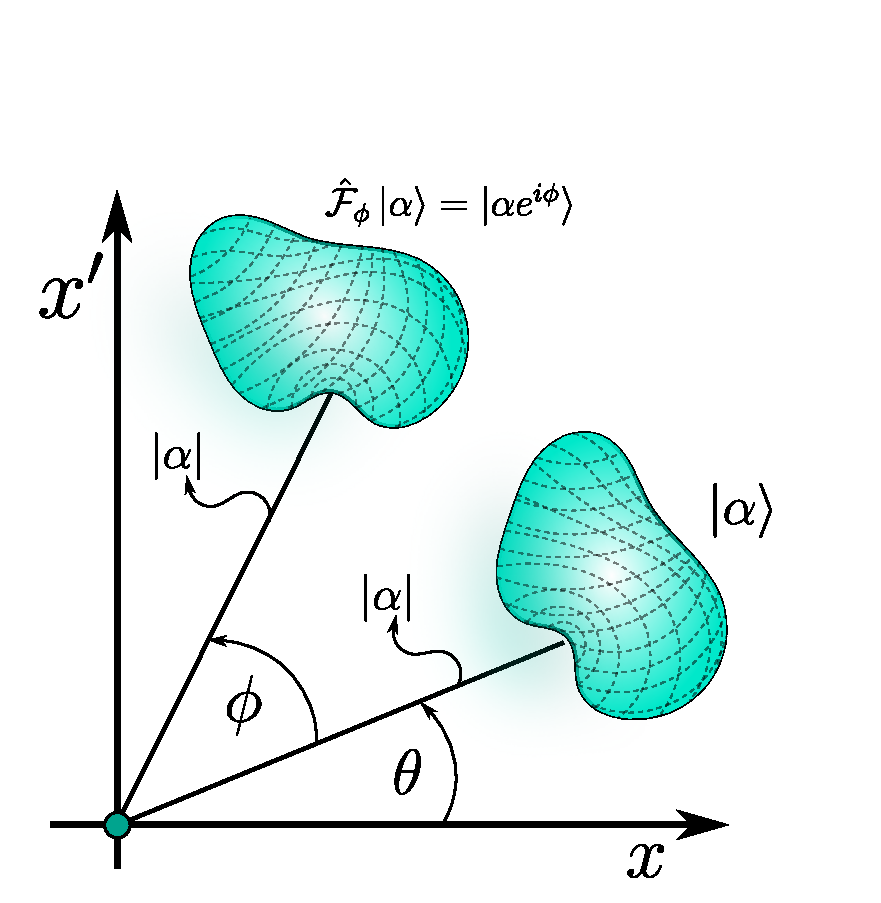
\includegraphics[width=0.75\linewidth]{Capitulo 7/Figuras/WignerRot.pdf}
            \caption{Efecto de la TFF sobre la distribución de Wigner en el espacio de fase de los estados coherentes $\ket{\alpha}$.}
            \label{fig:WignerRot}
        \end{figure}

        El interés principal para estudiar la TFF en el contexto de la fase cuántica es debido a su clara relación con los estados de fase  $\ket{\phi}$. Primero, vamos a definir los estados de fase cero como

        \begin{equation}
            \ket{\#} = \sum_{n=0}^\infty \ket{n},
        \end{equation}
        en donde podemos ver que si aplicamos la TFF sobre los estados de fase cero daremos lugar a los estados de fase como sigue

        \begin{equation}
            \hat{\mathcal{F}}_\phi \ket{\#} = e^{i\hat{N}\phi}\sum_{n=0}^{\infty}\ket{n} = \sum_{n=0}^\infty e^{in\phi}\ket{n} = \ket{\phi},
        \end{equation}
        entonces los estados $\ket{\#}$ y $\ket{\phi}$ son pares de una TFF (ver figura \ref{fig:PhaseRot}), por ende, la TFF produce una rotación de los estados de fase, esto es 

        \begin{equation}
            \hat{\mathcal{F}}_{\pm\theta}\ket{\phi} = \ket{\phi \pm \theta}.
        \end{equation}

        \begin{figure}[htbp]
            \centering
            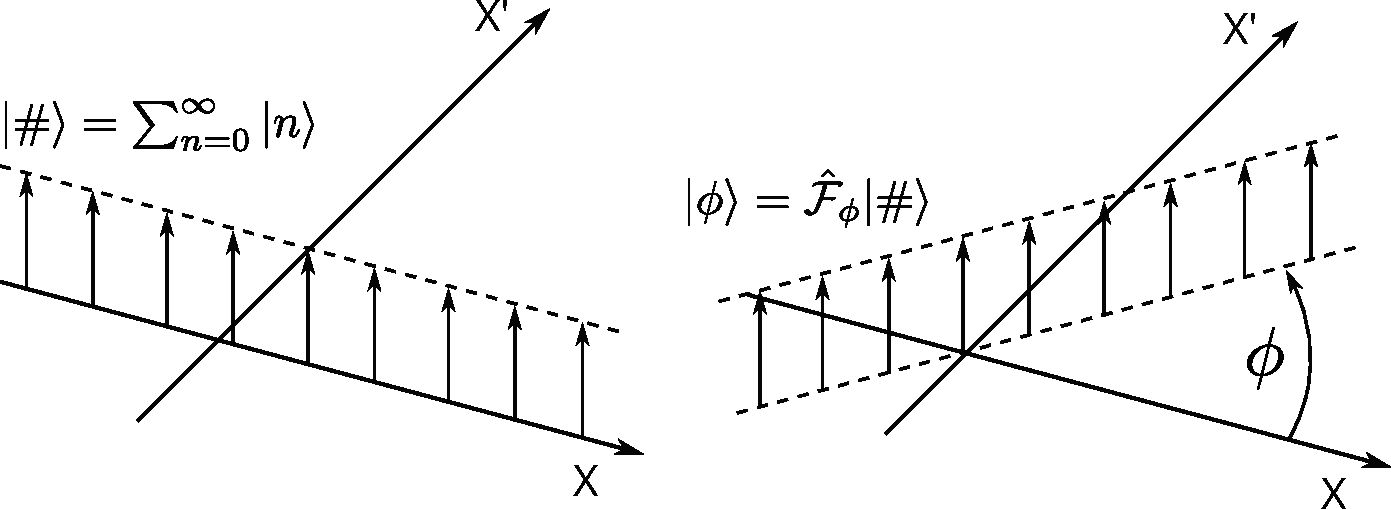
\includegraphics[width=\linewidth]{Capitulo 7/Figuras/PhaseRot.pdf}
            \caption{Representación gráfica de los estados de fase como la rotación de los estados numeral $\ket{\#}$}
            \label{fig:PhaseRot}
        \end{figure}

        Los estados de fase no forman una base ortogonal ya que un estado es deducido del otro por una rotación en el espacio de fase.

\section{Operador Exponencial de fase}

        Del operador exponencial de fase de Susskind-Glogower \ref{eq:SGNum} podemos ir definiendo las potencias del operador $\hat{E}$ de la siguiente manera

        \begin{align}
            & \hat{E}^2 = \sum_{n,n'=0}^\infty \ket{n}\braket{n+1|n'}\bra{n'+1} = \sum_{n,n'=0}^\infty\ket{n}\delta_{n'n+1}\bra{n'+1} = \sum_{n=0}^\infty \ket{n}\bra{n+2},\\
            & \hat{E}^{\dagger 2} = \sum_{n=0}^\infty \ket{n+2}\bra{n},
        \end{align}
        y, por inducción matemática, podemos probar que para cualquier $m \in \mathbb{Z}^+$ se cumple

        \begin{align}
            & \hat{E}^m = \sum_{n=0}^\infty \ket{n}\bra{n+m},\\
            & \left( \hat{E}^\dagger \right)^m = \sum_{n=0}^\infty \ket{n+m}\bra{n}.
        \end{align}

        Si tratamos de revisar la unitaridad del operador $\hat{E}^m$ vamos a llegar a una relación similar a la que se obtuvo con el operador de Susskind y Glogower, esto lo podemos demostrar de la siguiente manera

        \begin{align}\label{eq:VariosE}
            & \hat{E}^m \left( \hat{E}^\dagger \right)^m = \sum_{n,n'=0}^\infty \ket{n}\braket{n+m|n'+m}\bra{n'} = \sum_{n,n'=0}^\infty \ket{n}\delta_{nn'}\bra{n'} = \sum_{n=0}^\infty \ket{n}\bra{n}=\mathbb{I},\\
            & \left( \hat{E}^\dagger \right)^m \hat{E}^m = \sum_{n,n'=0}^\infty \ket{n+m}\braket{n|n'}\bra{n'+m} = \sum_{n,n'=0}^\infty\ket{n+m}\delta_{nn'}\bra{n'+m} = \mathbb{I}- \sum_{n=0}^{m-1}\ket{n}\bra{n},\\
            & \left[ \hat{E}^m, \left( \hat{E}^\dagger \right)^m \right] = \sum_{n=0}^{m-1}\ket{n}\bra{n},\\
            & \hat{E}^{-m} = \sum_{n=m}^\infty \ket{n}\bra{n-m} = \sum_{n=0}^\infty \ket{n+m}\bra{n} = \left( \hat{E}^\dagger \right)^m.
        \end{align}

        De lo anterior tenemos que el operador $\hat{E}^m$ es también semi-unitario, como se esperaría ya que este proviene del operador exponencial de fase de Susskind y Glogower, el cual ya era semi-unitario. Lo interesante está en que, mientras que para $m=1$, si $n$ es muy grande, el operador es aproximadamente unitario ya que el efecto del vacío cuántico puede llegar a ser despreciable, sin embargo, para el operador $\hat{E}^m$ podemos observar que esto no es válido, incluso cuando $m \to \infty$ el operador $\left( \hat{E}^\dagger \right)^m$ será ortogonal por izquierda al operador $\hat{E}^m$.

        Antes de seguir, es útil evaluar los siguientes conmutadores entre el exponencial de fase y el operador TFF como sigue

        \begin{align}
            & \left[ \hat{E}^m, \hat{\mathcal{F}}_\theta \right] = \sum_{n=0}^\infty \ket{n}\bra{n+m}\hat{\mathcal{F}}_\theta - \hat{\mathcal{F}}_\theta \sum_{n=0}^\infty \ket{n}\bra{n+m},\\
            & \left[ \hat{E}^m, \hat{\mathcal{F}}_\theta \right] = \sum_{n=0}^{\infty} e^{i(n+m)\theta}\ket{n}\bra{n+m} - \sum_{n=0}^{\infty} e^{in\theta} \ket{n}\bra{n+m},\\
            & \left[ \hat{E}^m, \hat{\mathcal{F}}_\theta \right] = \left( e^{im\theta} -1 \right)\sum_{n=0}^\infty e^{in\theta}\ket{n}\bra{n+m} = \left( e^{im\theta}-1 \right)\hat{\mathcal{F}}_\theta\hat{E}^m.
        \end{align}
        Con el operador adjunto conjugado tenemos una relación semejante

        \begin{equation}
            \left[ \left( \hat{E}^\dagger \right)^m, \hat{\mathcal{F}}_\theta \right] = \left( 1-e^{im\theta} \right)\left( \hat{E}^\dagger \right)^m \hat{\mathcal{F}}_\theta.
        \end{equation}

        De estas dos últimas relaciones de conmutación podemos llegar a las siguientes ecuaciones

        \begin{equation}
            \hat{\mathcal{F}}_\theta \left( \hat{E}^\dagger \right)^m \hat{\mathcal{F}}_\theta^\dagger = \left( \hat{E}^\dagger \right)^me^{im\theta}, \quad \hat{\mathcal{F}}_\theta \hat{E}^m \hat{\mathcal{F}}^\dagger_\theta = \hat{E}^m e^{-im\theta},
        \end{equation}
        y si aplicamos estos operadores sobre los estados de fase $\ket{\phi}$ tendremos

        \begin{equation}\label{eq:FFSimil}
            \hat{\mathcal{F}}_\theta \hat{E}^m \hat{\mathcal{F}}^\dagger_\theta \ket{\phi} = e^{im(\phi-\theta)}\ket{\phi}, \quad \hat{\mathcal{F}}_\theta \left( \hat{E}^\dagger \right)^m \hat{\mathcal{F}}_\theta^\dagger\ket{\phi} = e^{-im(\phi-\theta)}\ket{\phi}.
        \end{equation}

        En las ecuaciones \ref{eq:FFSimil} observamos que la transformación de similaridad de los operadores exponencial de fase en términos de la TFF nos lleva a un cambio de espacio de fase donde el estado de fase cero se ha modificado por $\phi = \theta$.

\section{Operador de fase cuántica}

        Con base en los estados numeral, podemos definir su proyector en los estados de fase cero como sigue

        \begin{equation}
            \ket{\#}\bra{\#} = \sum_{n,n'=0}^\infty \ket{n}\bra{n'} = \sum_{m=-\infty}^\infty \hat{E}^m
        \end{equation}
        y utilizando las ecuaciones \ref{eq:VariosE} tendremos
        \begin{equation}
            \ket{\#}\bra{\#} = \sum_{n=0}^\infty \ket{n}\bra{n} + \sum_{m=1}^\infty \left[ \hat{E}^m + \left( \hat{E}^\dagger \right)^m \right],
        \end{equation}
        entonces el operador proyector de fase será

        \begin{equation}
            \ket{\theta}\bra{\theta} = \hat{\mathcal{F}}_\theta \ket{\#}\bra{\#}\hat{\mathcal{F}}_\theta^\dagger = \sum_{n=0}^\infty \ket{n}\bra{n} + \sum_{m=1}^\infty \left[ \hat{\mathcal{F}}_\theta \hat{E}^m \hat{\mathcal{F}}_\theta^\dagger + \hat{\mathcal{F}}_\theta \left( \hat{E}^\dagger \right)^m \hat{\mathcal{F}}_\theta^\dagger \right],
        \end{equation}
        y usando las relaciones de similaridad encontradas en \ref{eq:FFSimil} tenemos que el proyector de fase es

        \begin{equation}\label{eq:FaseProy}
            \ket{\theta}\bra{\theta} = \sum_{n=0}^\infty\ket{n}\bra{n} + \sum_{m=1}^\infty \left[ \hat{E}^m e^{-im\theta} + \left( \hat{E}^\dagger \right)^me^{im\theta} \right].
        \end{equation}

        Vale la pena mencionar que el proyector $\hat{P}_\theta = \ket{\theta}\bra{\theta}$ al no conmutar con $\hat{E}^m$ hace que los estados de fase $\ket{\phi}$ no sean estados propios de $\hat{P}_\theta$.

        Debido a que los estados de fase no son ortogonales, vamos a adoptar la formulación de operadores Hermíticos de Toeplitz-Rosenblum \cite{rosenblum1962self}. Entonces para un $f: \Omega \subseteq \mathbb{R} \to \mathbb{R}$ una función Lebesgue-integrable, un operador hermítico puede ser definido en la forma

        \begin{equation}
            \hat{F}_\phi = \frac{1}{2\pi}\int_\phi ^{\phi + 2\pi} f(\theta) \ket{\theta}\bra{\theta}d\theta,
        \end{equation}
        para $f(\theta) = \theta$, tenemos el operador de Garrison y Wong \cite{garrison1970canonically}, y usando el proyector \ref{eq:FaseProy} tenemos

        \begin{align}
            & \hat{\Theta}_\phi = \frac{1}{2\pi}\int_\phi^{\phi+2\pi}\theta\ket{\theta}\bra{\theta}d\theta,\\
            & \hat{\Theta}_\phi = \sum_{n=0}^\infty \ket{n}\bra{n}\frac{1}{2\pi}\int_\phi^{\phi+2\pi} \theta d\theta + \sum_{m=1}^\infty \hat{E}^m\frac{1}{2\pi}\int_{\phi}^{\phi+2\pi}\theta e^{-im\theta}d\theta + \sum_{m=1}^\infty \left( \hat{E}^\dagger \right)^m \frac{1}{2\pi}\int_\phi^{\phi+2\pi}\theta e^{im\theta}d\theta,
        \end{align}
        usando
        \begin{equation}
            \frac{1}{2\pi}\int_{\phi}^{\phi+2\pi} \theta e^{\pm im\theta}d\theta = \mp \frac{i}{m}e^{\pm im\phi},
        \end{equation}
        entonces

        \begin{align}
            & \hat{\Theta}_\phi = (\phi+\pi) \sum_{n=0}^\infty \ket{n}\bra{n} + i \sum_{m=1}^\infty \frac{e^{-im\phi}}{m}\sum_{n=0}^\infty \ket{n}\bra{n+m} - i \sum_{m=1}^\infty \frac{e^{im\phi}}{m}\sum_{n=0}^\infty \ket{n+m}\bra{n}.
        \end{align}

        Antes de seguir, debemos tener en cuenta las siguientes ecuaciones

        \begin{align}
            & \hat{\mathcal{F}}_\phi \ket{n}\bra{n+m}\hat{\mathcal{F}}_\phi^\dagger = e^{-im\phi}\ket{n}\bra{n+m},\\
            & \hat{\mathcal{F}}_\phi \ket{n+m}\bra{n}\hat{\mathcal{F}}_\phi^\dagger = e^{im\phi}\ket{n+m}\bra{n},
        \end{align}
        entonces, finalmente, el operador Hermítico de fase se define como

        \begin{equation}
            \hat{\Theta}_\phi = (\phi + \pi) \sum_{n=0}^\infty \ket{n}\bra{n} + \hat{\mathcal{F}}_\phi \left[ \sum_{n=0}^\infty\sum_{m=1}^\infty i \frac{\ket{n}\bra{n+m} - \ket{n+m}\bra{n}}{m} \right]\hat{\mathcal{F}}_\phi^\dagger,
        \end{equation}
        y para el caso $\phi = - \pi$ tenemos
        \begin{equation}
            \hat{\Theta}_{-\pi} = \sum_{n=0}^\infty \sum_{m=1}^\infty \frac{i^{2m+1}}{m}\left( \ket{n}\bra{n+m} - \ket{n+m}\bra{n} \right).
        \end{equation}

        Debido a que los estados $\ket{\phi}$ no son ortogonales, el cuadrado del operador $\hat{\Theta}_\phi$ no puede ser formulado mediante potencias, sino que este se debe calcular mediante la formulación de Toeplitz-Rosenblum para $f(\theta) = \theta^2$, entonces

        \begin{align}
            & \hat{\Theta}_\phi^2 = \frac{1}{2\pi}\int_\phi^{\phi+2\pi} \theta^2 \ket{\theta}\bra{\theta}d\theta,\\
            & \hat{\Theta}_\phi^2 = \sum_{n=0}^\infty \ket{n}\bra{n}\frac{1}{2\pi}\int_\phi^{\phi+2\pi}\theta^2 d\theta + \sum_{m=1}^\infty \hat{E}^m \frac{1}{2\pi}\int_\phi^{\phi+2\pi} \theta^2 e^{-im\theta}d\theta + \sum_{m=1}^\infty\left( \hat{E}^\dagger \right)^m\frac{1}{2\pi}\int_\phi^{\phi+2\pi}\theta^2e^{im\theta}d\theta,
        \end{align}
        usando el siguiente resultado del cálculo integral
        \begin{equation}
            \frac{1}{2\pi}\int_\phi^{\phi+2\pi}\theta^2 e^{\pm im\theta}d\theta = 2 \left[ \frac{\mp i (\phi+\pi)}{m}+ \frac{1}{m^2} \right]e^{\pm i m\phi},
        \end{equation}
        entonces
        \begin{align}
            & \hat{\Theta}_\phi^2 = \left[ (\phi+\pi)^2 + \frac{\pi^2}{3} \right]\sum_{n=0}^\infty\ket{n}\bra{n} + 2(\phi+\pi)\hat{\mathcal{F}}_\phi \left[ \sum_{n=0}^\infty\sum_{m=1}^\infty i \frac{\ket{n}\bra{n+m} -\ket{n+m}\bra{n} }{m} \right]\hat{\mathcal{F}}_\phi^\dagger\\
            &  + 2\hat{\mathcal{F}}_\phi \left[ \sum_{n=0}^\infty\sum_{m=1}^\infty \frac{\ket{n}\bra{n+m} + \ket{n+m}\bra{n}}{m^2} \right]\hat{\mathcal{F}}_\phi^\dagger.
        \end{align}

        Como el ángulo inicial $\phi$ es arbitrario, podemos escoger a $\phi = -\pi$, entonces

        \begin{equation}
            \hat{\Theta}_{-\pi}^2 = \frac{\pi^2}{3}\sum_{n=0}^\infty \ket{n}\bra{n} + 2 \left[ \sum_{n=0}^\infty\sum_{m=1}^\infty \frac{i^{2m}}{m^2}\left(  \ket{n}\bra{n+m} + \ket{n+m}\bra{n} \right)\right].
        \end{equation}

        London \cite{london1926jacobischen,london1927winkelvariable} mostró que la fase y el número de fotones no están asociados con operadores canónicamente conjugados cuya relación de incertidumbre no puede ser formulado en términos de los operadores de posición y momento dados. En este orden de ideas, calculamos el conmutador $\left[ \hat{N},\hat{\Theta} \right]$ entonces

        \begin{align}
            & \hat{N}\hat{\Theta} = \sum_{k=0}^\infty k \ket{k}\bra{k} \sum_{n=0}^\infty \sum_{m=1}^\infty  \frac{i^{2m+1}}{m}\left( \ket{n}\bra{n+m} - \ket{n+m}\bra{n} \right),
        \end{align}


        \begin{align}
            & \hat{N}\hat{\Theta} = \sum_{n=0}^\infty\sum_{m=1}^\infty \frac{i^{2m+1}}{m}\left( n\ket{n}\bra{n+m} - (n+m)\ket{n+m}\bra{n} \right),\\
            & \hat{N}\hat{\Theta} = \sum_{n=0}^\infty\sum_{m=1}^\infty\frac{i^{2m+1}n}{m}\left( \ket{n}\bra{n+m} - \ket{n+m}\bra{n}\ \right) - \sum_{n=0}^\infty\sum_{m=1}^\infty i^{2m+1}\ket{n+m}\bra{n},
        \end{align}
        similarmente
        \begin{equation}
            \hat{\Theta}\hat{N}= \sum_{n=0}^\infty\sum_{m=1}^\infty \frac{i^{2m+1}n}{m} \left( \ket{n}\bra{n+m}-\ket{n+m}\bra{n} \right) + \sum_{n=0}^\infty \sum_{m=1}^\infty i^{2m+1}\ket{n}\bra{n+m},
        \end{equation}
        por ende el conmutador entre el número de fotones y el operador de fase será

        \begin{equation}
            \left[ \hat{N},\hat{\Theta} \right] = -i \sum_{n=0}^\infty\sum_{m=1}^\infty (-1)^m \left( \ket{n}\bra{n+m} + \ket{n+m}\bra{n} \right),
        \end{equation}
        con $\phi = -\pi$ tenemos
        \begin{equation}
            \sum_{n=0}^\infty\sum_{m=1}^\infty(-1)^m \left( \ket{n}\bra{n+m} + \ket{n+m}\bra{n} \right) = \ket{\pi}\bra{\pi} - \mathbb{I},
        \end{equation}
        finalmente el conmutador será

        \begin{equation}
            \left[ \hat{N},\hat{\Theta} \right] = i \left( \mathbb{I} - \ket{\pi}\bra{\pi} \right),
        \end{equation}
        donde el operador $\ket{\pi}\bra{\pi}$ corresponde a la función singular $\delta(\theta-\pi)$ (ver figura \ref{fig:chivsphi}). Entonces tenemos una relación de conmutación en la forma postulada por Judge y Lewis \cite{judge1963commutator}, donde $\hat{\Theta}$ es expresada como una función $2\pi$ periódica pero para nuestro caso de los operadores número y fase sin la necesidad de introducir operadores número negativos o espacios de Hilbert extendidos. 
\section{El operador de diferencia de fase cuántica y su relación con la polarización}

    Otra de las diferentes propuestas respecto a la formulación de la fase es la desarrollada por Alfredo Luis y Luis Sanchez Soto \cite{Diferencia-Fase}. En su artículo, resaltan el hecho de que la mayor parte del trabajo invertido en este problema se enfoca principalmente en las propiedades de un operador de fase para el campo electromagnético con un único modo de oscilación. Sin embargo, en un sentido práctico la noción de fase recupera mayor relevancia si se trata de una diferencia de fase entre una oscilación y otra que se tome de referencia, siendo esta una motivación para introducir lo que denominan un operador de diferencia de fase. \\ 
    
    
    En este sentido, se considera nuevamente un operador exponencial de fase $\hat{E}_{12}$, el cual ahora va a estar definido para un estado bimodal de campo $|n_1,n_2\rangle$, para lo cual se efectúa la descomposición polar 
    
    \begin{equation}
    \widehat{a}_{1}\widehat{a}^{\dagger}_2 = \hat{E}_{12}\sqrt{\hat{N}_1(\hat{N}_2 + 1)}.
    \end{equation}
    
    Sin embargo, esta relación no logra caracterizar por completo al operador $\hat{E}_{12}$, pues por ejemplo si deseamos estudiar el caso en el que la totalidad de fotones se encuentra en sólo uno de los modos, encontramos que los elementos de $\langle n_1,0| \hat{E}_{12} | 0,n_2\rangle$ no están definidos. Por lo que es necesario caracterizar otras condiciones para el operador, las cuales pueden ser obtenidas mediante la relación de conmutación con la acción $j$ del oscilador armónico, la cual puede entenderse como un momento angular. Para ello, clásicamente se sabe que satisface el corchete de Poisson
    
    \begin{equation}\label{eq:Poisson1}
        \{j,\phi\} = 1,
    \end{equation}
    y
    \begin{equation}\label{eq:Poisson2}
        \{j_1 + j_2,\phi_{12}\} = 0,
    \end{equation}
    \begin{equation}
        \left\{\frac{j_1 - j_2}{2},\phi_{12}\right\} = 1
    \end{equation}
    para el caso de dos osciladores independientes. De manera que para nuestros osciladores cuánticos tendríamos 
    \begin{equation}
        [E_{12},N_1+N_2] = 0,
    \end{equation}
    y 
    \begin{equation}
        \left[E_{12},\frac{N_1 - N_2}{2}\right] = E_{12}.
    \end{equation}
    Esta segunda ecuación se puede interpretar como el análogo al criterio de Lerner.

    Debe notarse que hay una solución no unitaria para $\hat{E}_{12}$ que verifica simultáneamente estas dos relaciones de conmutación y se le puede llamar como el operador exponencial de diferencia de fase de Susskind-Glogower. La falta de unitaridad de esta solución es un remanente de la incompatibilidad con una traducción cuántica de los corchetes de Poisson \ref{eq:Poisson1},\ref{eq:Poisson2}.

    Para proponer un operador de diferencia de fase vamos a tomar ventaja de que los siguientes operadores
    \begin{align}\label{eq:Jotas}
        & \hat{J}_x = \frac{1}{2}\left(  \hat{a}_1^\dagger \hat{a}_2 + \hat{a}_2^\dagger\hat{a}_1\right),\\
        & \hat{J}_y = \frac{i}{2}\left( \hat{a}_2^\dagger\hat{a}_1 - \hat{a}_1^\dagger\hat{a}_2 \right),\\
        & \hat{J}_z = \frac{1}{2}\left( \hat{a}_1^\dagger \hat{a}_1 - \hat{a}_2^\dagger\hat{a}_2 \right),
    \end{align}
    satisfacen las relaciones de conmutación del álgebra de Lie del grupo de rotaciones tridimensionales $SU(2)$:
    \begin{equation}
        \left[ \hat{J}_k, \hat{J}_l \right] = i \epsilon_{klm}\hat{J}_m.
    \end{equation}
    El invariante de Casimir para este grupo puede ser puesto en la forma
    \begin{equation}
        \hat{J}^2 = \frac{\hat{N}}{2}\left( \frac{\hat{N}}{2}+1 \right);
    \end{equation}
    de hecho, $\hat{N}$ conmuta con todos los operadores $\hat{J}_i\;,\; i=1,2,3$. El espacio de Hilbert total del problema $\mathcal{H}_1\otimes \mathcal{H}_2$ puede ser expresado como una suma directa de los subespacios invariantes bajo los operadores de momento angular
    \begin{equation}
        \mathcal{H}_1\otimes\mathcal{H}_2 = \bigoplus_{n=0}^\infty \mathcal{H}_n.
    \end{equation}

    Cada $\mathcal{H}_n$ tiene un número total de fotones $n$ fijo y es generado por los $2j+1=n+1$ vectores $\ket{j,m}$, los cuales son estados propios en común de $\hat{J}^2$ y $\hat{J}_z$. Los estados propios de número $\ket{n_1,n_2}\in \mathcal{H}_n$ corresponden a la base $\ket{j,m}$ como sigue

    \begin{equation}
        \ket{n_1,n_2} = \ket{j = (n_1+n_2)/2, m = (n_1-n_2)/2}.
    \end{equation}

    Podemos definir unos operadores escalera de momento angular $\hat{J}_\pm$ tales que

    \begin{align}
        & \hat{J}_+ = \hat{J}_x + i \hat{J}_y = \hat{a}_1^\dagger\hat{a}_2,\\
        & \hat{J}_- = \hat{J}_x -i\hat{J}_y = \hat{a}_1\hat{a}_2^\dagger,
    \end{align}
    en donde podemos ver la relación entre $\hat{J}_\pm$ y el operador exponencial de diferencia de fase $\hat{E}_{12}$ como

    \begin{equation}\label{eq:JE12}
        \hat{J}_- = \hat{E}_{12}\sqrt{\hat{J}_+\hat{J}_-}.
    \end{equation}

    Debido a que el operador $\hat{E}_{12}$ conmuta con el número total de fotones $\hat{N}$ entonces vamos a restringir un poco el estudio a cada subespacio $\mathcal{H}_n$ y, posteriormente, extender esto al espacio de Hilbert completo. Sea $\hat{E}_{12}^{(n)}$ la restricción, entonces la ecuación \ref{eq:JE12} se puede resolver obteniendo el operador exponencial de diferencia de fase unitario $SU(2)$ como

    \begin{equation}\label{eq:E12Jotas}
        \hat{E}_{12}^{(n)} = \sum_{m=-j+1}^j \ket{j,m-1}\bra{j,m}+e^{i(n+1)\phi^{(n)}}\ket{j,j}\bra{j,-j},
    \end{equation}
    siendo $\phi^{(n)}$ una fase arbitraria. Nótese que el término extra en \ref{eq:E12Jotas} es importante ya que garantiza la unitaridad de $\hat{E}_{12}^{(n)}$ y se sostiene en la finitud de los estados número. Para los operadores del oscilador armónico tal descomposición es inviable porque sus estados número se extienden hacia el infinito y no tiene un término extra que proyecte un estado superior a un estado base ( a menos de que uno decida truncar como en el formalismo de Pegg-Barnett). De esta manera, en cada subespacio $\mathcal{H}_n$ hay $n+1$ estados ortonormales que verifican

    \begin{equation}
        \hat{E}_{12}^{(n)}\ket{\phi_r^{(n)}} = e^{i\phi_r^{(n)}}\ket{\phi_r^{(n)}},
    \end{equation}
    con $r=0,...,n.$ Estos estados se pueden expresar en la base de los estados número como

    \begin{equation}
        \ket{\phi_r^{(n)}} = \frac{1}{\sqrt{n+1}} \sum_{n_1=0}^n e^{in_1\phi_r^{(n)}}\ket{n_1,n-n_1},
    \end{equation}
    donde, al tomar la misma ventana de $2\pi$ en cada subespacio, tenemos
    \begin{equation}
        \phi_r^{(n)} = \phi_0 + \frac{2\pi r}{n+1}.
    \end{equation}

    La expresión para $\hat{E}_{12}$ en todo el espacio se obtiene al tomar las infinitas copias del exponencial de diferencia de fase de $SU(2)$
    \begin{align}
        & \hat{E}_{12} = \sum_{n=0}^\infty \hat{E}_{12}^{(n)} = \sum_{n=0}^\infty \sum_{r=0}^n \ket{\phi_r^{(n)}}e^{i\phi_r^{(n)}}\bra{\phi_r^{(n)}},\\
        & \hat{E}_{12} = \sum_{n=0}^\infty \frac{1}{n+1}\sum_{r=0}^n \sum_{k,k'=0}^n \ket{k,n-k}e^{i\left( k-k'+1 \right)\phi_r^{(n)}}\bra{k',n-k'}.
    \end{align}

    Como $\hat{E}_{12}$ es unitario, este define un operador de diferencia de fase hermítico
    \begin{equation}
        \hat{\phi}_{12} = \sum_{n=0}^\infty \sum_{r=0}^n \ket{\phi_r^{(n)}}\phi_r^{(n)}\bra{\phi_r^{(n)}},
    \end{equation}
    y finalmente tenemos $\hat{E}_{12} = e^{i\hat{\phi}_{12}}$.

    Este operador difiere de otros, principalmente porque no se puede obtener de una construcción previa de los operadores de fase para cada uno de los osciladores individuales involucrados. Además, a diferencia del formalismo de Susskind-Glogower, $\hat{E}_{12}$ así definido sí es unitario.

    A su vez, el espectro de valores propios de $\hat{\phi}_{12}$ es discreto, para cada subespacio $\mathcal{H}_n$ hay $n+1$ uniformemente distribuidos valores propios en el intervalo $[0,2\pi]$, a diferencia de otros formalismos que dan un espectro continuo en el intervalo $[0,4\pi]$.

    Podemos dar una interpretación física a los operadores de momento angular y al operador de diferencia de fase en términos de la polarización. Una forma de lidiar con la polarización a nivel cuántico es con los operadores de Stokes definidos por

    \begin{align}
        &\hat{S}_0 = \hat{a}_1^\dagger\hat{a}_1 + \hat{a}_2^\dagger\hat{a}_2,\\
        & \hat{S}_1 = \hat{a}_1^\dagger\hat{a}_2 + \hat{a}_2^\dagger\hat{a}_1,\\
        & \hat{S}_2 = i\left( \hat{a}_2^\dagger\hat{a}_1 - \hat{a}_1^\dagger\hat{a}_2 \right),\\
        & \hat{S}_3 = \hat{a}_1^\dagger \hat{a}_1 - \hat{a}_2^\dagger \hat{a}_2.
    \end{align}

    Nótese que, excepto por un factor de $2$, los operadores $\hat{S}_i\;,\; i=1,2,3$ coinciden con los operadores \ref{eq:Jotas} de momento angular, mientras que $\hat{S}_0$ representa el número total de fotones $\hat{N}$. La no conmutatividad de los operadores de Stokes nos advierte sobre la imposibilidad de hacer mediciones simultáneas de las cantidades físicas asociadas a estos operadores. Los operadores $\hat{S}_i$ pueden ser vistos como generadores de un grupo de transformaciones localmente isomorfas al grupo de rotaciones tridimensional que dejan invariante al operador $\hat{S}_0$.

    Estos operadores de Stokes replican los parámetros de Stokes cuando calculamos los valores medios en la base de los estados coherentes bimodales dados por
    \begin{equation}
        \ket{\alpha_1,\alpha_2} = e^{-\frac{|\alpha_1|^2+|\alpha_2|^2}{2}}\sum_{n_1,n_2=0}^\infty \frac{\alpha_1^{n_1}\alpha_2^{n_2}}{\sqrt{n_1! n_2!}}\ket{n_1,n_2},
    \end{equation}
    en donde los parámetros de Stokes se calculan como

    \begin{align}
        & s_0 = \bra{\alpha_1,\alpha_2}\hat{S}_0 \ket{\alpha_1,\alpha_2} = |\alpha_1|^2 + |\alpha_2|^2,\\
        & s_1 = \bra{\alpha_1,\alpha_2}\hat{S}_1 \ket{\alpha_1,\alpha_2} = 2|\alpha_1||\alpha_2|\cos(\phi_1-\phi_2), \\
        & s_2 = \bra{\alpha_1,\alpha_2}\hat{S}_2 \ket{\alpha_1,\alpha_2} = -2|\alpha_1||\alpha_2|\sin(\phi_1-\phi_2), \\
        & s_3 = \bra{\alpha_1,\alpha_2}\hat{S}_3 \ket{\alpha_1,\alpha_2} = |\alpha_1|^2 - |\alpha_2|^2.
    \end{align} 

    Si denotamos como $s_\pm = (s_1\pm is_2)/2$ entonces la diferencia de fase clásica entre dos modos se obtiene sin ambigüedades como

    \begin{equation}
        s_+ = e^{-i(\phi_1-\phi_2)}|\alpha_1||\alpha_2| = e^{-i(\phi_1-\phi_2)}\sqrt{s_-s_+}.
    \end{equation}

    \chapter{La propoagación fundamental de los fotones}
	\thispagestyle{empty}
	\vspace*{2cm}
	\begin{center}
		{\itshape\Huge \par}
		\vspace{1cm}
		\epigraph{``El fotón es emitido aquí, absorbido allá, y entre esos puntos no sabemos —ni podemos saber— qué camino siguió. La naturaleza solo exige que la suma de todos los caminos posibles contribuya a la probabilidad final''}{-- Richard Feynman }
	\end{center}
	\clearpage

	\section{La idea de Feynman y la construcción del propagador}

    En una fiesta en la taberna Nassau de Princeton, en la primavera de 1941, un físico visitante llamado Herbert Jehle le preguntó a Feynman en qué andaba trabajando. Feynman le contó que estaba buscando una formulación de la mecánica cuántica construida sobre el lagrangiano y no sobre el hamiltoniano, y Jehle le respondió que eso ya estaba hecho, que Dirac había escrito un artículo sobre el asunto. A la mañana siguiente fueron juntos a la biblioteca, encontraron el trabajo de 1933 \citep{dirac1933lagrangian}, y Feynman leyó la frase que lo cambiaría todo: la amplitud de transición en un intervalo infinitesimal \textit{corresponde} a la exponencial de la acción dividida por $\hbar$. Feynman le preguntó a Jehle qué quería decir Dirac con la palabra corresponde, y Jehle contestó que los físicos ingleses la usaban vagamente. Feynman decidió averiguar, allí mismo y en el pizarrón, si corresponde no querría decir simplemente que son iguales salvo una constante. Descubrió que sí. Jehle, según el propio Feynman, se puso a tomar notas frenéticamente \citep{feynman1966development}.

    Lo que salió de esa mañana es el objeto que este capítulo usa para describir la propagación de los fotones. En el capítulo dedicado a la mecánica analítica ya obtuvimos la integral de camino por la vía corta, insertando relaciones de completitud dentro del operador de evolución, y allí nos limitamos a citar el prefactor sin deducirlo. Vale la pena rehacer el camino como lo recorrió Feynman, es decir, empezando por un experimento de interferencia y terminando en una fórmula, porque ese recorrido usa únicamente mecánica clásica, integrales gaussianas y series de Fourier, y porque al final nos dejará el prefactor calculado y no citado.

    \subsection{De la doble rendija a la suma sobre caminos}

        El punto de partida es el experimento más simple que exhibe comportamiento cuántico. Una fuente emite partículas hacia una pantalla con dos rendijas, y detrás hay un detector en el punto $b$. Si solo está abierta la rendija $1$, el detector registra una distribución $P_{1}$; si solo está abierta la $2$, registra $P_{2}$; y con ambas abiertas no registra $P_{1}+P_{2}$ sino un patrón de franjas. La regla que reproduce lo observado, y que en el capítulo de los postulados escribimos como regla de Born, consiste en asociar a cada alternativa un número complejo, sumar los números y elevar al cuadrado el módulo de la suma,
        \begin{equation}\label{eq:DosRendijas}
            \phi = \phi_{1} + \phi_{2}, \qquad P = \left|\phi_{1}+\phi_{2}\right|^{2} \neq \left|\phi_{1}\right|^{2} + \left|\phi_{2}\right|^{2} .
        \end{equation}
        El término cruzado que sobra al desarrollar el módulo al cuadrado es la interferencia, y todo el contenido del experimento está en que las amplitudes se suman antes de elevarse al cuadrado y no después.

        El salto de Feynman consiste en preguntarse qué ocurre si perforamos más agujeros. Con tres rendijas la amplitud es $\phi = \phi_{1}+\phi_{2}+\phi_{3}$, y con un número arbitrario de ellas
        \begin{equation}\label{eq:MuchasRendijas}
            \phi = \sum_{h} \phi_{h},
        \end{equation}
        donde el índice recorre los agujeros. Si ahora los agujeros se hacen tan numerosos y tan juntos que la pantalla desaparece, la suma se convierte en una integral sobre la posición $x$ en el plano de la pantalla, y el resultado debe ser el mismo que si la pantalla nunca hubiera estado allí, porque una pantalla con infinitos agujeros no es una pantalla.

        El paso siguiente es el que decide el asunto. Con dos pantallas en lugar de una, cada una con sus agujeros, la partícula debe atravesar un agujero de la primera y otro de la segunda para llegar al detector, y como esas son alternativas distintas, sus amplitudes se suman,
        \begin{equation}\label{eq:DosPantallas}
            \phi = \sum_{h_{1}}\sum_{h_{2}} \phi_{h_{1}h_{2}} .
        \end{equation}
        Con $N$ pantallas tendremos $N$ sumas encajadas, y si volvemos a hacer los agujeros infinitamente numerosos en cada una y las pantallas infinitamente numerosas a lo largo del camino, cada sumando queda especificado por la lista de puntos por los que la partícula pasó en cada instante intermedio. Pero una lista de posiciones, una por cada instante, es precisamente lo que en mecánica clásica llamamos una trayectoria. Hemos llegado, sin postular nada, al enunciado que da nombre al método: \textbf{la amplitud total es la suma de las amplitudes de todos los caminos concebibles que unen el punto de partida con el de llegada}, incluidos los que ningún cuerpo clásico recorrería jamás.

        Queda por decir cuánto vale la amplitud de cada camino, y aquí es donde Feynman postula que todos los caminos contribuyen con el mismo módulo y difieren únicamente en la fase, y que esa fase es la acción del camino medida en unidades de $\hbar$,
        \begin{equation}\label{eq:PostuladoFeynman}
            \phi[x(s)] = \text{const}\times \exp\left\{\frac{i}{\hbar}S[x(s)]\right\},
            \qquad
            S[x(s)] = \int_{0}^{t} L\left(x,\dot{x}\right) ds .
        \end{equation}

        Que el módulo sea el mismo para todos es una hipótesis de simetría razonable, pues no hay nada que distinga a un camino de otro salvo su forma. Que la fase sea la acción, en cambio, no es arbitrario y puede argumentarse desde la mecánica clásica, que es lo que nos interesa. Si la fase fuese una funcional cualquiera $\Phi[x]$ del camino, podríamos determinarla así. Cuando el sistema es macroscópico sabemos cuál debe ser el resultado, a saber, que la partícula sigue la trayectoria que hace estacionaria la acción; y la única manera de que una suma de números complejos de módulo igual reproduzca ese resultado es que las fases de los caminos vecinos al clásico coincidan entre sí, es decir, que $\Phi$ sea estacionaria exactamente donde lo es $S$. La elección más simple compatible con esa exigencia es que $\Phi$ sea proporcional a $S$, y la constante de proporcionalidad debe tener dimensiones inversas a las de la acción para que la fase sea un número puro. En la naturaleza solo hay una constante con dimensiones de acción, de modo que $\Phi = S/\hbar$.

        El mecanismo por el cual esa suma reproduce la mecánica clásica es puramente geométrico. Tomemos dos caminos vecinos, uno el clásico y otro que se aparta de él en una cantidad pequeña. Sus acciones difieren, y sus contribuciones a la suma son dos números complejos de igual módulo cuyas fases difieren en $\Delta S/\hbar$. Si esa diferencia de fase es grande comparada con $2\pi$, los dos números apuntan en direcciones esencialmente aleatorias y al sumarse se cancelan; si es pequeña, apuntan casi en la misma dirección y se refuerzan. Con números: para un grano de polvo de un miligramo que se mueve un centímetro en un segundo, la acción es del orden de
        \begin{equation}\label{eq:EstimacionClasica}
            S \sim m v L \sim \left(10^{-6}\,\mathrm{kg}\right)\left(10^{-2}\,\mathrm{m\,s^{-1}}\right)\left(10^{-2}\,\mathrm{m}\right) = 10^{-10}\,\mathrm{J\,s},
        \end{equation}
        que en unidades de $\hbar\approx 10^{-34}\,\mathrm{J\,s}$ vale unos $10^{24}$ radianes. Desviar el camino en una millonésima de milímetro cambia la acción en una parte minúscula, pero esa parte minúscula sigue siendo del orden de $10^{15}$ radianes, de manera que la contribución del camino desviado apunta en una dirección completamente arbitraria respecto de la del camino original. La cancelación es feroz, y solo sobrevive la vecindad del camino para el cual la acción es estacionaria, porque allí, y solo allí, la acción no cambia a primer orden y las fases vecinas coinciden. Para un electrón atado a un átomo, en cambio, la acción típica es del orden de $\hbar$ mismo, no hay cancelación, y todos los caminos cuentan. En esta observación está contenida la respuesta a la objeción que se le hizo a Fermat en el siglo XVII: la luz no escoge el camino de tiempo estacionario, los recorre todos, y el camino estacionario es simplemente aquel cuyos vecinos no lo cancelan.

        Para convertir lo anterior en una fórmula usable necesitamos una definición y una propiedad. La definición es la del \textit{propagador} o núcleo, que es la amplitud de que una partícula que estaba en $x_{I}$ en el instante cero sea hallada en $x_{F}$ en el instante $t$, y que escribimos $K(x_{F},t;x_{I},0)$. Con ella, el conocimiento de la función de onda en un instante determina la de cualquier otro instante, porque las alternativas se suman y el punto de partida es una alternativa más,
        \begin{equation}\label{eq:EvolucionK}
            \psi(x_{F},t) = \int_{\mathbb{R}} K(x_{F},t;x_{I},0)\,\psi(x_{I},0)\,dx_{I} .
        \end{equation}
        Esta expresión es la razón por la cual el propagador nos interesa aquí: tiene exactamente la forma de una integral de difracción, con el núcleo haciendo el papel del factor de propagación y la función de onda inicial el de la amplitud en el plano del objeto. Que esa semejanza sea una coincidencia formal o algo más profundo es el asunto del resto del capítulo.

        La propiedad que necesitamos es la ley de composición. Si la partícula va de $a$ a $b$ pasando por un instante intermedio, debe pasar por algún punto $x_{c}$ en ese instante, y como pasar por un punto o por otro son alternativas mutuamente excluyentes, mientras que recorrer el primer tramo y luego el segundo son sucesos consecutivos, las amplitudes de los tramos se multiplican y las de los puntos intermedios se suman,
        \begin{equation}\label{eq:Composicion}
            K(x_{F},t_{2};x_{I},t_{0}) = \int_{\mathbb{R}} K(x_{F},t_{2};x_{c},t_{1})\,K(x_{c},t_{1};x_{I},t_{0})\,dx_{c} .
        \end{equation}
        Nótese que \eqref{eq:Composicion} no es un postulado adicional sino una consecuencia directa de la suma sobre caminos: partir el conjunto de todos los caminos según el punto por el que cruzan un instante dado, y sumar primero dentro de cada grupo y después sobre los grupos, es simplemente reordenar la suma. La acción, por su parte, se parte igual de bien, pues es una integral en el tiempo y $S_{\text{total}} = S_{\text{primer tramo}} + S_{\text{segundo tramo}}$, de modo que la exponencial del total es el producto de las exponenciales.

        Podemos ahora aplicar \eqref{eq:Composicion} $N$ veces, dividiendo el intervalo $[0,t]$ en $N$ tramos iguales de duración
        \begin{equation}\label{eq:Epsilon}
            \varepsilon = \frac{t}{N},
            \qquad
            t_{j} = j\varepsilon,
            \qquad
            x_{j} = x(t_{j}),
        \end{equation}
        con $x_{0}=x_{I}$ y $x_{N}=x_{F}$ fijos. Componiendo tramo a tramo,
        \begin{equation}\label{eq:Rodajas}
            K(x_{F},t;x_{I},0) = \int\cdots\int \prod_{j=1}^{N-1}dx_{j}\;\prod_{j=0}^{N-1} K\left(x_{j+1},t_{j+1};x_{j},t_{j}\right),
        \end{equation}
        y ahora cada factor se refiere a un intervalo infinitesimal, que es donde el postulado \eqref{eq:PostuladoFeynman} puede aplicarse sin ambigüedad. En un tramo tan corto la partícula no tiene tiempo de hacer nada complicado, de manera que su velocidad puede tomarse constante e igual al cociente incremental y el potencial puede evaluarse en el extremo del tramo,
        \begin{equation}\label{eq:AccionTramo}
            S_{j} = \int_{t_{j}}^{t_{j+1}} L\,ds \approx \varepsilon\left[\frac{m}{2}\left(\frac{x_{j+1}-x_{j}}{\varepsilon}\right)^{2} - V(x_{j})\right],
        \end{equation}
        con un error de orden $\varepsilon^{2}$ que desaparece en el límite. El propagador infinitesimal es entonces
        \begin{equation}\label{eq:NucleoCorto}
            K\left(x_{j+1},t_{j+1};x_{j},t_{j}\right) = \frac{1}{A}\exp\left\{\frac{i\varepsilon}{\hbar}\left[\frac{m}{2}\left(\frac{x_{j+1}-x_{j}}{\varepsilon}\right)^{2} - V(x_{j})\right]\right\},
        \end{equation}
        donde $A$ es la constante de normalización que Dirac había dejado sin determinar y que vamos a calcular ahora.

    \subsection{La constante de normalización y la partícula libre}

        La manera más económica de fijar $A$ consiste en exigir que la ley de composición \eqref{eq:Composicion} se cumpla, porque esa ley no admite constantes sobrantes. Hagámoslo con la partícula libre, para la cual $V=0$, y compongamos dos tramos de duración $\varepsilon$ para ver si el resultado tiene la forma de un solo tramo de duración $2\varepsilon$.

        Antes necesitamos una integral que usaremos sin descanso a lo largo de todo el cálculo. Se trata de la integral gaussiana con exponente imaginario, llamada integral de Fresnel, cuyo valor es
        \begin{equation}\label{eq:Fresnel}
            \int_{-\infty}^{\infty} e^{i a u^{2}}\,du = \sqrt{\frac{i\pi}{a}}\,,
            \qquad a \in \mathbb{R}\setminus\{0\},
        \end{equation}
        y que se obtiene de la gaussiana ordinaria $\int e^{-\beta u^{2}}du = \sqrt{\pi/\beta}$ por continuación analítica, sustituyendo $\beta = -ia$ y entendiendo el resultado como el límite de una gaussiana con parte real positiva infinitesimal, que es lo que garantiza la convergencia. La raíz de $i$ vale $e^{i\pi/4}$, de modo que la integral de Fresnel no es más que una gaussiana con un desfase de un octavo de vuelta.

        Vamos a componer los dos tramos. Escribiendo $x_{0}$, $x_{1}$ y $x_{2}$ para los tres puntos y usando \eqref{eq:NucleoCorto} con $V=0$,
        \begin{equation}\label{eq:ComposicionLibre1}
            K_{2} = \frac{1}{A^{2}}\int_{-\infty}^{\infty}\exp\left\{\frac{im}{2\hbar\varepsilon}\left[\left(x_{2}-x_{1}\right)^{2} + \left(x_{1}-x_{0}\right)^{2}\right]\right\}dx_{1},
        \end{equation}
        y todo el trabajo consiste en hacer esa integral, que es gaussiana en la variable intermedia. Desarrollemos el corchete agrupando las potencias de $x_{1}$,
        \begin{equation}\label{eq:ComposicionLibre2}
            \left(x_{2}-x_{1}\right)^{2} + \left(x_{1}-x_{0}\right)^{2}
            = 2x_{1}^{2} - 2x_{1}\left(x_{0}+x_{2}\right) + x_{0}^{2} + x_{2}^{2},
        \end{equation}
        y completemos el cuadrado en $x_{1}$ sumando y restando el término que hace falta,
        \begin{equation}\label{eq:ComposicionLibre3}
            2x_{1}^{2} - 2x_{1}\left(x_{0}+x_{2}\right)
            = 2\left[x_{1}^{2} - x_{1}\left(x_{0}+x_{2}\right) + \textcolor{blue}{\frac{\left(x_{0}+x_{2}\right)^{2}}{4}}\right] - \textcolor{blue}{\frac{\left(x_{0}+x_{2}\right)^{2}}{2}}
            = 2\left[x_{1}-\frac{x_{0}+x_{2}}{2}\right]^{2} - \frac{\left(x_{0}+x_{2}\right)^{2}}{2},
        \end{equation}
        donde los dos términos en azul se han introducido a propósito y su contribución neta es nula. Los términos que ya no dependen de $x_{1}$ salen fuera de la integral, y lo que queda dentro es exactamente la integral de Fresnel \eqref{eq:Fresnel} con $a = m/\hbar\varepsilon$,
        \begin{equation}\label{eq:ComposicionLibre4}
            \int_{-\infty}^{\infty}\exp\left\{\frac{im}{\hbar\varepsilon}\left[x_{1}-\frac{x_{0}+x_{2}}{2}\right]^{2}\right\}dx_{1} = \sqrt{\frac{i\pi\hbar\varepsilon}{m}} = \sqrt{\frac{2\pi i\hbar\varepsilon}{2m}} .
        \end{equation}
        Reuniendo los factores de fuera, y usando que
        \begin{equation}\label{eq:ComposicionLibre5}
            x_{0}^{2}+x_{2}^{2} - \frac{\left(x_{0}+x_{2}\right)^{2}}{2} = \frac{2x_{0}^{2}+2x_{2}^{2}-x_{0}^{2}-2x_{0}x_{2}-x_{2}^{2}}{2} = \frac{\left(x_{2}-x_{0}\right)^{2}}{2},
        \end{equation}
        el resultado de componer los dos tramos es
        \begin{equation}\label{eq:ComposicionLibre6}
            K_{2} = \frac{1}{A^{2}}\sqrt{\frac{\pi i\hbar\varepsilon}{m}}\;\exp\left\{\frac{im\left(x_{2}-x_{0}\right)^{2}}{2\hbar\left(2\varepsilon\right)}\right\} .
        \end{equation}

        Este es el punto que decide la constante. La exponencial de \eqref{eq:ComposicionLibre6} es exactamente la de un único tramo de duración $2\varepsilon$, tal como exige la ley de composición, de manera que el postulado de Feynman pasa la prueba sin necesidad de ajustar nada. Para que también el prefactor tenga la forma de un solo tramo, es decir, para que sea el mismo $1/A$ pero con $\varepsilon$ reemplazado por $2\varepsilon$, hace falta que
        \begin{equation}\label{eq:CondicionA}
            \frac{1}{A^{2}(\varepsilon)}\sqrt{\frac{\pi i \hbar \varepsilon}{m}} = \frac{1}{A(2\varepsilon)},
        \end{equation}
        y basta probar con $A(\varepsilon) = C\sqrt{\varepsilon}$ para ver que la condición se satisface si $C = \sqrt{2\pi i\hbar/m}$. La constante de normalización queda así determinada,
        \begin{equation}\label{eq:ConstanteA}
            A(\varepsilon) = \sqrt{\frac{2\pi i\hbar\varepsilon}{m}},
        \end{equation}
        y con ella el propagador infinitesimal \eqref{eq:NucleoCorto} está completamente especificado. Lo que Dirac había llamado \textit{corresponde} era, en efecto, una igualdad, y la constante que faltaba es la de \eqref{eq:ConstanteA}.

        El propagador de la partícula libre para un tiempo finito se obtiene ahora sin esfuerzo, porque el cálculo que acabamos de hacer se repite idéntico en cada composición. Componer dos tramos de duración $\varepsilon$ dio un tramo de duración $2\varepsilon$ con la misma forma funcional; componer ese con otro da uno de duración $3\varepsilon$, y así sucesivamente. Por inducción, tras $N$ composiciones,
        \begin{equation}\label{eq:PropagadorLibre}
            K_{\text{libre}}(x_{F},t;x_{I},0) = \sqrt{\frac{m}{2\pi i\hbar t}}\;\exp\left\{\frac{im\left(x_{F}-x_{I}\right)^{2}}{2\hbar t}\right\},
        \end{equation}
        que es un resultado exacto y no una aproximación, porque el error de orden $\varepsilon^{2}$ que cometimos en \eqref{eq:AccionTramo} se anula cuando el potencial es nulo.

        Merece atención el exponente de \eqref{eq:PropagadorLibre}. La trayectoria clásica de una partícula libre que va de $x_{I}$ a $x_{F}$ en un tiempo $t$ es la recta recorrida con velocidad constante $v = (x_{F}-x_{I})/t$, y su acción vale
        \begin{equation}\label{eq:AccionLibre}
            S_{\mathrm{cl}} = \int_{0}^{t}\frac{m}{2}v^{2}\,ds = \frac{m}{2}\frac{\left(x_{F}-x_{I}\right)^{2}}{t^{2}}\,t = \frac{m\left(x_{F}-x_{I}\right)^{2}}{2t},
        \end{equation}
        de manera que \eqref{eq:PropagadorLibre} se lee $K = \sqrt{m/2\pi i\hbar t}\,e^{iS_{\mathrm{cl}}/\hbar}$. La suma sobre infinitos caminos ha dado como resultado la exponencial de la acción de uno solo de ellos, el clásico, multiplicada por un factor que no depende de los extremos. Esto no es una casualidad ni es exclusivo de la partícula libre, y la sección siguiente explica por qué.

    \subsection{Sistemas cuadráticos y el propagador del oscilador}

        Supongamos que el lagrangiano es un polinomio de grado dos en la posición y la velocidad, que es el caso de la partícula libre, del oscilador armónico y de la partícula en un campo uniforme. Podemos separar cada camino en el clásico más una desviación que se anula en los extremos, puesto que todos los caminos comparten los mismos puntos inicial y final,
        \begin{equation}\label{eq:SeparacionCamino}
            x(s) = x_{\mathrm{cl}}(s) + y(s),
            \qquad y(0)=y(t)=0 .
        \end{equation}
        Al sustituir en la acción y desarrollar, aparecen tres tipos de términos: los que no contienen $y$, que reconstruyen $S_{\mathrm{cl}}$; los lineales en $y$, que se anulan idénticamente porque la acción es estacionaria sobre el camino clásico, que es el principio de Hamilton del capítulo de mecánica analítica; y los cuadráticos en $y$, que por ser el lagrangiano de grado dos no dependen ya de $x_{\mathrm{cl}}$. Es decir,
        \begin{equation}\label{eq:AccionSeparadaFey}
            S[x] = S_{\mathrm{cl}} + \textcolor{red}{\left(\text{términos lineales en } y\right)} + S_{2}[y] = S_{\mathrm{cl}} + S_{2}[y],
        \end{equation}
        donde el término marcado en rojo se anula por la estacionariedad. Como los extremos de $y$ están fijos en cero, sumar sobre todos los caminos $x$ equivale a sumar sobre todas las desviaciones $y$, y el factor $e^{iS_{\mathrm{cl}}/\hbar}$ sale fuera de esa suma por no depender de la variable de integración. Resulta entonces que
        \begin{equation}\label{eq:FormaCuadratica}
            K(x_{F},t;x_{I},0) = F(t)\,\exp\left\{\frac{i}{\hbar}S_{\mathrm{cl}}(x_{F},t;x_{I},0)\right\},
        \end{equation}
        con un prefactor $F(t)$ que depende del tiempo transcurrido pero no de dónde se empieza ni de dónde se termina. La aproximación semiclásica es exacta para estos sistemas, y el problema de calcular un propagador se parte en dos piezas independientes: una de mecánica clásica pura, que es hallar $S_{\mathrm{cl}}$, y una de integración gaussiana, que es hallar $F(t)$.

        La primera pieza ya la tenemos. En el capítulo de mecánica analítica calculamos la acción clásica del oscilador armónico imponiendo los extremos $q(0)=q_{I}$ y $q(t)=q_{F}$, y el resultado fue
        \begin{equation}\label{eq:AccionOsciladorAqui}
            S_{\mathrm{cl}} = \frac{m\omega}{2}\left[\left(q_{I}^{2}+q_{F}^{2}\right)\cot\omega t - \frac{2q_{I}q_{F}}{\sin\omega t}\right].
        \end{equation}

        La segunda pieza es la que quedó pendiente allí y la que vamos a calcular aquí, y lo haremos con una herramienta que es de mecánica clásica y no de teoría cuántica de campos: los modos normales. La desviación $y(s)$ es una función que se anula en $s=0$ y en $s=t$, exactamente como el desplazamiento de una cuerda sujeta por los dos extremos, de manera que admite un desarrollo en la serie de senos correspondiente,
        \begin{equation}\label{eq:SerieSenos}
            y(s) = \sum_{n=1}^{\infty} a_{n}\sin\left(\frac{n\pi s}{t}\right),
        \end{equation}
        y sumar sobre todos los caminos de desviación equivale a integrar sobre todos los valores posibles de los coeficientes $a_{n}$. Este cambio de variables convierte una integral funcional, que es un objeto incómodo, en un producto de integrales ordinarias, que no lo es.

        En estas variables, $S_{2}[y]$ se calcula sin dificultad. Para el oscilador,
        \begin{equation}\label{eq:S2Oscilador}
            S_{2}[y] = \int_{0}^{t}\left(\frac{m}{2}\dot{y}^{2} - \frac{m\omega^{2}}{2}y^{2}\right)ds,
        \end{equation}
        y necesitamos las dos integrales de los productos de senos y cosenos, que son las relaciones de ortogonalidad de siempre,
        \begin{equation}\label{eq:OrtogonalidadSenos}
            \int_{0}^{t}\sin\left(\frac{n\pi s}{t}\right)\sin\left(\frac{n'\pi s}{t}\right)ds = \frac{t}{2}\delta_{nn'},
            \qquad
            \int_{0}^{t}\cos\left(\frac{n\pi s}{t}\right)\cos\left(\frac{n'\pi s}{t}\right)ds = \frac{t}{2}\delta_{nn'} .
        \end{equation}
        Derivando \eqref{eq:SerieSenos} término a término, $\dot{y} = \sum_{n} a_{n}(n\pi/t)\cos(n\pi s/t)$, y sustituyendo ambas series en \eqref{eq:S2Oscilador}, las deltas de \eqref{eq:OrtogonalidadSenos} colapsan las dobles sumas en sumas simples,
        \begin{equation}\label{eq:S2Diagonal}
            S_{2} = \frac{m}{2}\cdot\frac{t}{2}\sum_{n=1}^{\infty}\left(\frac{n\pi}{t}\right)^{2}a_{n}^{2} - \frac{m\omega^{2}}{2}\cdot\frac{t}{2}\sum_{n=1}^{\infty}a_{n}^{2}
            = \frac{mt}{4}\sum_{n=1}^{\infty}\left[\left(\frac{n\pi}{t}\right)^{2}-\omega^{2}\right]a_{n}^{2} .
        \end{equation}
        La acción de las fluctuaciones ha quedado diagonal: no hay términos cruzados entre modos distintos, y cada coeficiente aparece elevado al cuadrado y multiplicado por un número. Esta es la razón por la cual los modos normales son la variable correcta, y es el mismo motivo por el que lo son en la cuerda vibrante o en la cavidad del capítulo anterior.

        La integral sobre las fluctuaciones se factoriza entonces en un producto de integrales de Fresnel independientes, una por cada modo,
        \begin{equation}\label{eq:ProductoFresnel}
            F(t) = J \prod_{n=1}^{\infty}\int_{-\infty}^{\infty}\exp\left\{\frac{imt}{4\hbar}\left[\left(\frac{n\pi}{t}\right)^{2}-\omega^{2}\right]a_{n}^{2}\right\}da_{n}
            = J\prod_{n=1}^{\infty}\sqrt{\frac{4\pi i\hbar}{mt\left[\left(n\pi/t\right)^{2}-\omega^{2}\right]}},
        \end{equation}
        donde $J$ recoge el jacobiano del cambio de variables entre las posiciones intermedias y los coeficientes $a_{n}$, junto con los factores $1/A$ de la medida. Ese $J$ es incómodo y, tomado por separado, ni siquiera es finito; pero tiene una virtud decisiva, y es que no depende de $\omega$, puesto que el cambio de variables \eqref{eq:SerieSenos} no sabe nada del potencial. Podemos por tanto deshacernos de él comparando el oscilador con la partícula libre, cuyo prefactor ya conocemos de \eqref{eq:PropagadorLibre}. Dividiendo \eqref{eq:ProductoFresnel} por la misma expresión evaluada en $\omega = 0$, el jacobiano se cancela y también lo hacen todos los factores constantes de cada modo,
        \begin{equation}\label{eq:Cociente}
            \frac{F_{\omega}(t)}{F_{0}(t)} = \prod_{n=1}^{\infty}\sqrt{\frac{\left(n\pi/t\right)^{2}}{\left(n\pi/t\right)^{2}-\omega^{2}}}
            = \prod_{n=1}^{\infty}\left[1 - \frac{\omega^{2}t^{2}}{n^{2}\pi^{2}}\right]^{-1/2} .
        \end{equation}

        El producto infinito que ha aparecido es conocido desde Euler. Se trata de la factorización del seno en términos de sus ceros,
        \begin{equation}\label{eq:ProductoEuler}
            \frac{\sin z}{z} = \prod_{n=1}^{\infty}\left(1 - \frac{z^{2}}{n^{2}\pi^{2}}\right),
        \end{equation}
        que puede entenderse sin dificultad: el miembro derecho se anula exactamente en $z = \pm n\pi$, que son los ceros del seno distintos del origen, y vale uno en $z=0$, igual que el izquierdo. Identificando $z = \omega t$, el producto de \eqref{eq:Cociente} es precisamente $\sin(\omega t)/(\omega t)$ elevado a la potencia $-1/2$, de manera que
        \begin{equation}\label{eq:CocienteFinal}
            \frac{F_{\omega}(t)}{F_{0}(t)} = \sqrt{\frac{\omega t}{\sin\omega t}} .
        \end{equation}
        Sustituyendo el prefactor libre $F_{0}(t) = \sqrt{m/2\pi i\hbar t}$, los dos factores de $t$ se cancelan y queda
        \begin{equation}\label{eq:PrefactorOscilador}
            F_{\omega}(t) = \sqrt{\frac{m}{2\pi i\hbar t}}\sqrt{\frac{\omega t}{\sin\omega t}} = \sqrt{\frac{m\omega}{2\pi i\hbar\sin\omega t}} .
        \end{equation}

        Reuniendo \eqref{eq:AccionOsciladorAqui} y \eqref{eq:PrefactorOscilador} en la forma general \eqref{eq:FormaCuadratica} obtenemos el propagador del oscilador armónico,
        \begin{equation}\label{eq:PropagadorOsciladorFeynman}
            K(q_{F},t;q_{I},0) = \left(\frac{m\omega}{2\pi i\hbar\sin\omega t}\right)^{1/2}
            \exp\left\{\frac{i m\omega}{2\hbar}\left[\left(q_{I}^{2}+q_{F}^{2}\right)\cot\omega t - \frac{2q_{I}q_{F}}{\sin\omega t}\right]\right\},
        \end{equation}
        deducido sin más herramientas que la suma sobre caminos, el principio de Hamilton, unas integrales gaussianas y una serie de Fourier.

        Antes de seguir podemos verificar dos límites. Cuando la frecuencia tiende a cero, usando $\sin\omega t\to\omega t$ y $\cot\omega t\to 1/\omega t$, el prefactor tiende a $\sqrt{m/2\pi i\hbar t}$ y el exponente a $im(q_{I}^{2}+q_{F}^{2}-2q_{I}q_{F})/2\hbar t$, que es la partícula libre \eqref{eq:PropagadorLibre}, como debía ser. Cuando $\omega t$ se acerca a un múltiplo de $\pi$, en cambio, el prefactor diverge, y esa divergencia no es un defecto del cálculo sino un hecho físico: transcurrido medio período todas las trayectorias que salieron de $q_{I}$ vuelven a reunirse en el mismo punto, de modo que la amplitud se concentra allí. Son los puntos conjugados que ya encontramos al calcular la acción clásica, y su análogo óptico es el foco de un sistema formador de imagen.

        Queda por decir cómo se conecta esto con el fotón, que es de lo que trata el capítulo. En el capítulo dedicado a la cuantización vimos que el campo electromagnético encerrado en una cavidad es dinámicamente equivalente a una colección de osciladores armónicos independientes, uno por cada modo, y que las variables canónicas de cada modo están normalizadas de manera que la masa efectiva vale la unidad. Poniendo $m=1$ en \eqref{eq:PropagadorOsciladorFeynman} se obtiene
        \begin{equation}\label{eq:PropagadorModo}
            K(q_{F},t;q_{I},0) = \left(\frac{\omega}{2\pi i\hbar\sin\omega t}\right)^{1/2}
            \exp\left\{\frac{i\omega}{2\hbar}\left[\left(q_{I}^{2}+q_{F}^{2}\right)\cot\omega t - \frac{2q_{I}q_{F}}{\sin\omega t}\right]\right\},
        \end{equation}
        que es exactamente la amplitud de transición de la que parte la sección siguiente. El resto del capítulo consiste en tomar en serio la forma de esta expresión, que combina una fase cuadrática en los dos extremos con un término cruzado, y reconocer en ella el núcleo de una transformada de Fourier fraccionaria y, por tanto, una integral de difracción de Fresnel.

\section{Propagador de fotones}

    En esta parte vamos a abordar la naturaleza de la propagación de los fotones y su relación con el principio de Huygens-Fresnel. Aunque el uso de la fórmula de difracción de Rayleigh-Sommerfeld como propagador de fotones es ampliamente aceptado debido a la evidencia experimental disponible, aún existen interrogantes sobre la conexión directa entre la propagación del campo electromagnético en la óptica clásica y la propagación de los fotones, donde el cuadrado de la amplitud de probabilidad describe la probabilidad transversal de detección del fotón.

    Además, se presenta una formulación matemática para la propagación de los fotones utilizando el formalismo de la cuantización del campo electromagnético y el método de la integral de camino. Esta formulación tiene una similitud destacada con una transformada de Fourier fraccional (FRFT, por sus siglas en inglés). Se demuestra que debido a la estrecha relación existente entre la FRFT y la integral de difracción de Fresnel, este propagador puede expresarse como una difracción de Fresnel, lo que plantea una discusión sobre su carácter fundamental a nivel de fotón en comparación con el principio de Huygens-Fresnel.
    
    Finalmente, se realiza un experimento de conteo de fotones utilizando una rendija rectangular, confirmando que el fenómeno de difracción en la aproximación de Fresnel se comporta de manera similar al límite clásico real.
    \subsection{Propagador de fotón}
    
    La amplitud de transición correspondiente para el Hamiltoniano de un campo electromagnético cuantizado es calculada mediante el método de la integral de trayectoria:
    
    \begin{equation}
        \left < q_{F} \left | e^{-i\hat{H}t/\hbar} \right | q_{I} \right > = \left ( \frac{\omega}{2\pi i \hbar \sin (\omega t)} \right ) ^{\frac{1}{2}} \exp \left \{  \frac{i}{2\hbar}\omega  \left [ \left (  q_{I}^{2}+q_{F}^{2} \right ) \cot (\omega t) - \frac{2q_{I}q_{F}}{\sin (\omega t)} \right ] \right \}
    \end{equation}
    
    Entonces, la evolución temporal de un sistema en un estado $\left | \psi  \right >$ en la representación de $q$ se escribe:
    
    \begin{equation}
        \psi(q_{F},t)= \left ( \frac{\omega}{2\pi i \hbar \sin (\omega t)} \right ) ^{\frac{1}{2}} \int _{\mathbb{R}} \psi (q_{I},0) \exp \left \{  \frac{i}{2\hbar}\omega  \left [ \left (  q_{I}^{2}+q_{F}^{2} \right ) \cot (\omega t) - \frac{2q_{I}q_{F}}{\sin (\omega t)} \right ] \right \} dq_{I}
        \label{propagfoton}
    \end{equation}
    Esta ecuación describe cómo evoluciona en el tiempo la “función de onda” a medida que se propaga la luz, cuyo núcleo se escribe como una transformada de Fourier y una fase cuadrática al igual que la integral de difracción de Fresnel en la propagación clásica del campo electromagnético. Esta similitud nos permite establecer una conexión donde la integral de difracción de Fresnel juega un papel importante en la propagación de fotones.
    
    \subsection{Propagador del campo electromagnético clásico}
    
    La integral de difracción de Fresnel en una dimensión, a una distancia $z$, en el marco de la óptica metaxial de Bonnet se escribe:
    
    \begin{equation}
        U(x,z) = \left ( \frac{i}{\lambda z} \right )^{\frac{1}{2}} e^{ikz} \exp \left [ -\frac{ik}{2}\left ( \frac{1}{z} + \frac{1}{R_{B}}\right )x^{2} \right ]\int_{\Sigma }  \exp \left [ -\frac{ik}{2}\left ( \frac{1}{z} - \frac{1}{R_{A}}\right )x'^{2} \right ] \exp\left [ \frac{ik}{z}xx' \right ] U(x',0) dx'
        \label{eqfresnel}
    \end{equation}
    
    Donde las ondas esféricas se aproximan a parabólicas y el radio de curvatura para $U$ desde su vértice hasta el centro se define como la cantidad algebraica $R_{A} = \overline{VC}$, y se considera positivo si va en la dirección de propagación de la luz. 
    
    \begin{figure}[htbp]
        \centering    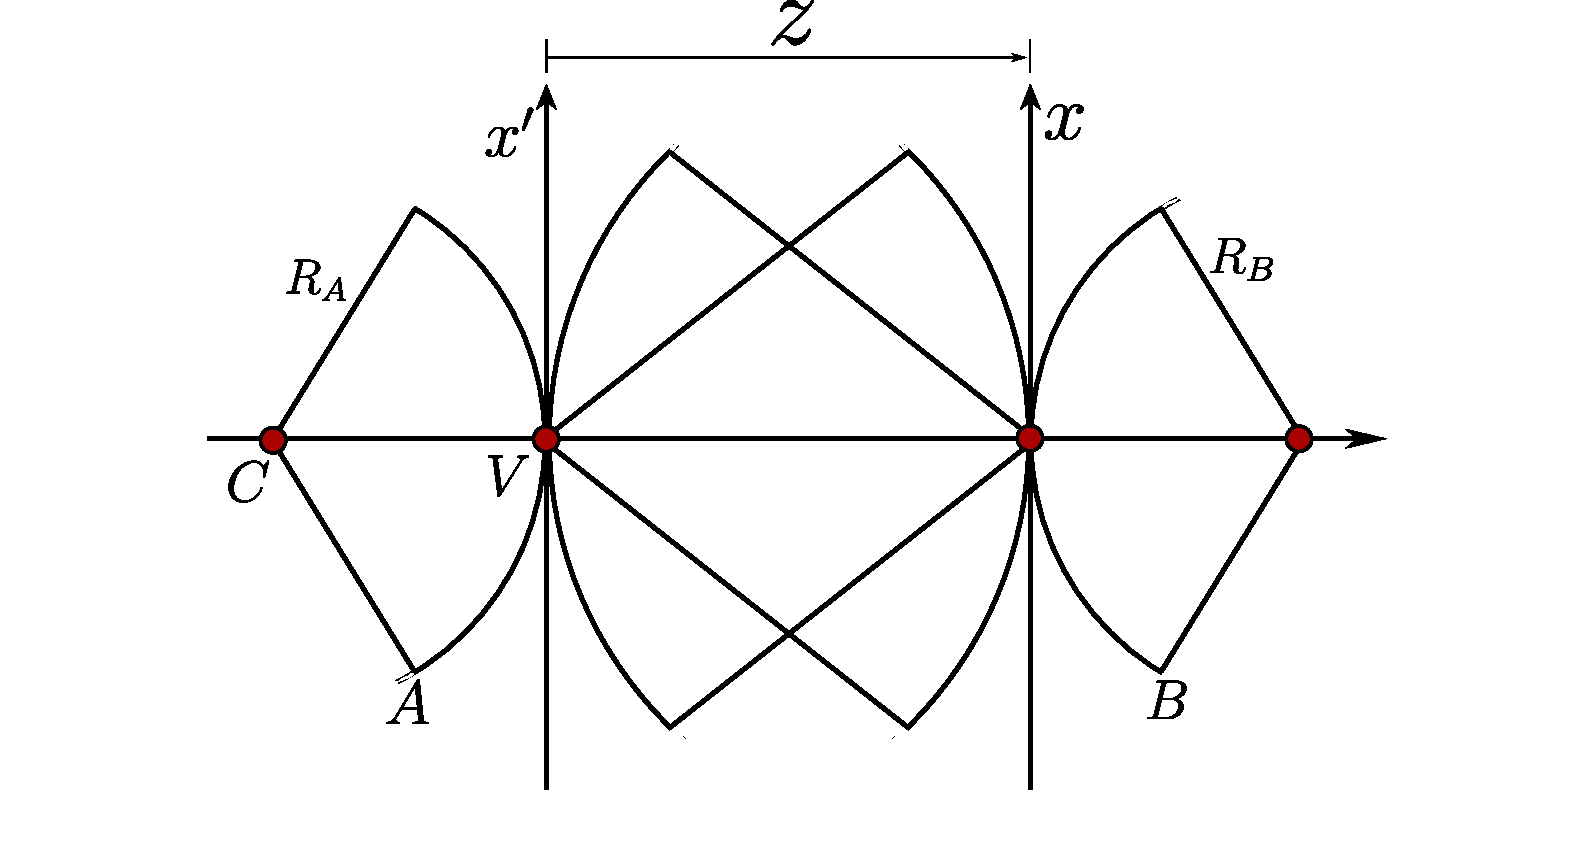
\includegraphics[width=0.9\textwidth]{Capitulo 8/Figuras/difraccionfresnel.pdf}
        \caption{Difracción de Fresnel entre la superficie esférica $A$ y la superficie esférica $B$.}
        \label{fig:difraccionfresnel}
    \end{figure}
    
    Pellat-Finet estableció una relación entre la difracción de Fresnel y la transformación de Fourier fraccionaria. Escribiendo las amplitudes del campo y las variables reducidas:
    
    \begin{equation}
        V_{A}(\rho) = U_{A}(\sqrt{\lambda \varepsilon R_{A}}\rho)\, ,\hspace{0.7cm} 
        V_{B}(\sigma) = U_{B}\left ( \frac{\sqrt{\lambda \varepsilon R_{A}}\sigma}{\cos \alpha + \varepsilon \sin \alpha} \right )
    \end{equation}
    \begin{equation}        
        \rho = \frac{1}{\sqrt{\lambda \varepsilon R_{A}}}x'\, ,\hspace{0.7cm}
        \sigma = \frac{1}{\sqrt{\lambda \varepsilon R_{A}}}(\cos \alpha + \varepsilon \sin \alpha)x
        \label{variablered}
    \end{equation}
    
    Dónde 
    \begin{equation}
        \cot \alpha = \varepsilon \frac{1-\mu}{\mu}\hspace{0.7cm} \mathrm{y} \hspace{0.7cm} \mu = \frac{z}{R_{A}}
        \label{eqcot}
    \end{equation}
    \begin{equation}
        \sin ^{2} \alpha = \frac{\mu ^{2}}{\mu ^{2} + \varepsilon ^{2} (1-\mu)^{2}}
        \label{eqsin}
    \end{equation}
    Además $\varepsilon$ es la solución en número real distinta de cero de:
    
    \begin{equation}
        \frac{1}{R_{B}} + \frac{1}{z} = \frac{\varepsilon^{2}(1-\mu)}{\mu R_{A}[\mu^{2} + \varepsilon^{2}(1-\mu)^{2}]}
        \label{eqradios}
    \end{equation}
    
    La ecuación $\ref{eqfresnel}$ se reescribe de la forma:
    
    \begin{equation}
        V_{B}(\sigma) = \frac{i}{\sin\alpha} (\cos \alpha + \varepsilon \sin \alpha) \int_{\mathbb{R}} V_{A}(\rho) \exp \left [ i\pi (\rho^{2}+ \sigma^{2})\cot \alpha - \frac{2i\pi \sigma \rho}{\sin \alpha} \right ] d\rho
        \label{tffr}
    \end{equation}
    
    Con esto, la relación entre el propagador de fotones $(\ref{propagfoton})$ y la integral de difracción de Fresnel escrita en la forma de la ecuación $\ref{tffr}$ es más clara. Solo se necesita encontrar el factor de escala para las variables reducidas apropiadas para $q_{I}$ y $q_{F}$.
    
    \subsection{Propagación como una integral de Fresnel}
    
    Para establecer una relación entre el propagador $(\ref{propagfoton})$ y la transformada de Fourier fraccionaria, se realiza el siguiente cambio de variables:
    
    \begin{equation}
        \rho^{2} = \frac{\omega}{2 \pi \hbar} q_{I}^{2}\, ,\hspace{0.7cm}
        \sigma^{2} = \frac{\omega}{2 \pi \hbar} q_{F}^{2}
    \end{equation}
    
    Usando $\alpha = wt$, $k = \frac{2\pi}{\lambda}$, $ct=\varepsilon R_{A}>0$ y difiniendo un término de masa $m_{\lambda} = \frac{\hbar k}{c}$ que está relacionado con el Hamiltoniano, es decir, el campo electromagnético cuantizado puede entenderse como un oscilador armónico mecánico cuántico con masa $m_{\lambda}$.
    
    \begin{equation}
        \rho^{2} = \frac{1}{\lambda \varepsilon R_{A}} \frac{\alpha}{m_{\lambda}} q_{I}^{2}\, ,\hspace{0.7cm}
        \sigma^{2} = \frac{1}{\lambda \varepsilon R_{A}} \frac{\alpha}{m_{\lambda}}  q_{F}^{2}
    \end{equation}
    
    Luego, usando las expresiones en $(\ref{variablered})$ se encuentra que la escala entre el observable $q$ y una posición real $x$ es:
    
    \begin{equation}
        x_{I}^{2} = \frac{\alpha}{m_{\lambda}}q_{I}^{2} \, ,\hspace{0.7cm}
        x_{F}^{2} = \frac{\alpha}{m_{\lambda}}q_{F}^{2}
    \end{equation}
    
    Donde 
    \begin{equation}
        \cos \alpha + \varepsilon \sin \alpha = 1
        \label{eqcos}
    \end{equation}
    
    Entonces la ecuación $\ref{propagfoton}$ se puede escribir de la forma:
    
    \begin{equation}
        \Psi(x_{F},t) = \left ( \frac{\omega}{2i\pi \hbar \sin (\omega t)} \right )^{\frac{1}{2}}\left ( \frac{m_{\lambda}}{\alpha} \right ) ^{\frac{1}{2}} \int_{\mathbb{R}} \psi(x_{I},0) \exp \left \{ \frac{i\pi}{\lambda \varepsilon R_{A}} \left [ \left ( x_{I}^{2} + x_{F}^{2} \right ) \cot \alpha - \frac{2 x_{I} x_{F}}{\sin \alpha} \right ]\right \} dx_{I}
        \label{propagador3}
    \end{equation}
    
    Con 
    \begin{equation}
        \Psi(x_{I},0) = \psi \left ( \sqrt{\frac{m_{\lambda}}{\alpha}}x_{I},0 \right ) \hspace{0.7cm} \mathrm{y} \hspace{0.7cm} \Psi(x_{F},t) = \psi \left ( \sqrt{\frac{m_{\lambda}}{\alpha}}x_{F},t \right )
    \end{equation}
    
    Además, usando $\ref{eqcot}$ y $\ref{eqcos}$ se llega a:
    
    \begin{equation}
        \sin \alpha = \frac{\mu}{\varepsilon}
        \label{eqsin2}
    \end{equation}
    
    Entonces, igualando $\ref{eqsin}$ y $\ref{eqsin2}$ se tiene:
    
    \begin{equation}
        \mu ^{2} + \varepsilon ^{2} (1-\mu)^{2} = \varepsilon ^{2}
    \end{equation}
    
    Con $\varepsilon ^{2} = \frac{\mu}{2- \mu}$. Entonces la ecuación $\ref{eqradios}$ toma la forma:
    
    \begin{equation}
        \frac{1}{R_{B}} + \frac{1}{z} = \frac{1-\mu}{\mu R_{A}}
    \end{equation}
    
    Finalmente, teniendo $R_{B} = -R_{A}$ la expresión $(\ref{propagador3})$ se puede escribir explícitamente en términos de la posición y la distancia de propagación $z$ como
    
    \begin{equation}
        \psi(x_{F},z) = \left ( \frac{i}{\lambda z} \right )^{\frac{1}{2}} \exp \left [ -\frac{ik}{2} \left ( \frac{1}{z} + \frac{1}{R_{B}} \right ) x_{F}^{2}  \right ] \int_{\Sigma} \exp \left [ -\frac{ik}{2} \left ( \frac{1}{z} - \frac{1}{R_{A}} \right ) x_{I}^{2}  \right ] \exp \left [ \frac{ik}{z} x_{I} x_{F} \right ] \psi (x_{I},0) dx_{I}
        \label{eq:fresnelclasica}
    \end{equation}
    
    La cual, es exactamente la fórmula clásica de difracción de Fresnel eliminando el factor de fase $e^{ikz}$. Además, se puede escribir en términos de las variables reducidas $\rho$ y $\sigma$ como la transformada de Fourier fraccionaria,
    
    \begin{equation}
        \phi (\sigma) = \left ( \frac{1}{i \sin \alpha} \right )^{\frac{1}{2}} \int_{\mathbb{R}} \exp \left \{ i \pi \left [ \left ( \rho^{2} + \sigma^{2} \right ) \cot \alpha - \frac{2 \rho \sigma}{\sin \alpha} \right ] \right \} \phi (\rho) d \rho
        \label{eq:FRFT}
    \end{equation}
    
    De esta manera, la $FRFT$ expresa matemáticamente la propagación de fotones de la misma forma que se emplea para propagar el campo clásico en el régimen de Fresnel. Se debe tener en cuenta que cuando $\alpha = \frac{\pi}{2}$, la propagación se convierte en la transformada de Fourier estándar (régimen de Fraunhofer). Lo notable aquí es que ahora disponemos de una herramienta ampliamente reconocida para estudiar la propagación de fotones, y podemos aplicar todas las propiedades del análisis de Fourier a la óptica cuántica. \\
    
    Como podemos ver, la función de onda $\Psi(x,t)$ se comporta como una función de onda de campo eléctrico que está estrechamente relacionada por algunos factores de escala con la función de onda $\psi(x,t)$ en la representación $q$ y se puede propagar de la misma manera como la integral de difracción de Fresnel clásica. Dado que en ambos casos —cuántico y clásico— la amplitud de probabilidad y la amplitud del campo eléctrico evolucionan de la misma manera, esto significa que el observable $q$ puede considerarse como una posición en la dirección transversal a la propagación del campo y paralela a la dirección de propagación de polarización del campo eléctrico. \\
    
    Por lo tanto, la ecuación $(\ref{propagfoton})$ representaría la evolución de la amplitud de probabilidad transversal, $\psi(x,t)$, de detectar un fotón, quedando deslocalizado longitudinalmente. Esto significa que el observable $\hat{q}$ está lejos de lo que puede considerarse como la posición del fotón. Vale la pena mencionar que no existe un operador de posición para fotones y no existe una descripción mecánica cuántica satisfactoria para el fotón en el sentido habitual.
    
    
    \subsection{Correspondencia a la teoría de la difracción escalar}
    
    ¿Es posible que la difracción de Fresnel no sea una simple aproximación a la fórmula de Rayleigh-Sommerfeld sino que describa de manera fundamental la propagación del campo de radiación? A continuación se mostrará cómo se puede ajustar la teoría de la difracción escalar para obtener una expresión diferente de un campo propagado. \\
    Se propone que el campo electromagnético no puede estar confinado en una región puntual sino en un pequeño volumen. No es muy instintivo pensar en una fuente puntual para una onda electromagnética o fotones ya que la densidad de energía espacial sería infinita. Por ejemplo, en la Ref. [33], los autores demuestran que las fuentes secundarias de Huygen tienen una dimensión y una densidad de energía finitas; además, se ha demostrado [30] que los fotones no se pueden localizar de forma nítida, aunque se ha estudiado la posibilidad de tener pulsos monofotónicos de área cero [34]. Por lo tanto, consideramos que cualquier fuente de ondas electromagnéticas $U(r,t)$ con longitud de onda $\lambda$ debe tener una amplitud constante en una vecindad de al menos el orden de la longitud de onda. Ahora bien, recordemos que en la teoría escalar de la difracción se utiliza el teorema de Green para calcular la propagación del campo electromagnético [1,2,26]. Se desea resolver, para $U$, la expresión:
    
    \begin{equation}
        \int_{V} U(\nabla ^{2} + k^{2}) G dv = \int_{S} \left ( U \frac{\partial G}{\partial n} - G \frac{\partial U}{\partial n} \right ) ds
        \label{intgreen}
    \end{equation}
    
    dónde $G$ es una función auxiliar, conocida como función de Green.
    
    \begin{equation}
        (\nabla^{2} + k^{2})'G_{\pm}(\vec{r}, \vec{r'}) = -4\pi [\delta(\vec{r} - \vec{r'}) \pm \delta(\vec{r} - \widetilde{\vec{r'}})]
        \label{condgreen}
    \end{equation}
    
    que representa una fuente puntual en $\vec{r'}$ $\in$ $V$ y $\widetilde{\vec{r'}}$ $\notin$ $V$. Esto permite el cálculo del campo $U$ en la región $V$ del espacio a la derecha del plano [Fig. $\ref{ftesferica}$]. Una solución para $G$, en el sentido de distribuciones, corresponde a la onda esférica,
    
    \begin{equation}
        G_{\pm} (\vec{r}, \vec{r'}) = \frac{e^{ik\left | \vec{r} - \vec{r'} \right |}}{\left | \vec{r} - \vec{r'} \right |} \pm \frac{e^{ik\left | \vec{r} - \widetilde{\vec{r'}} \right |}}{\left | \vec{r} - \widetilde{\vec{r'}} \right |}
    \end{equation}
    
    \begin{figure}[htbp]
    \centering
        \subfloat[]{
        \label{ftesferica}
        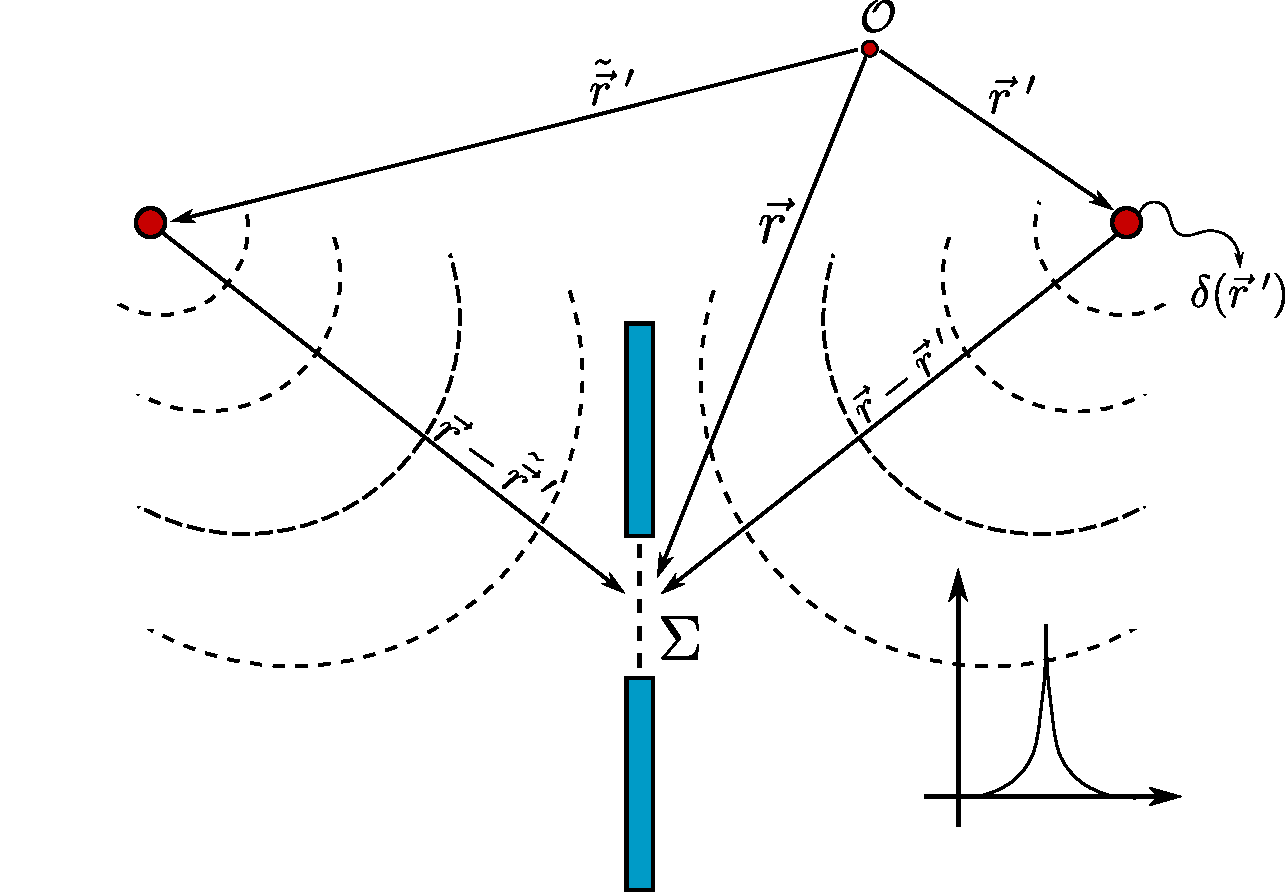
\includegraphics[width=0.5\textwidth]{Capitulo 8/Figuras/ftesferica.pdf}}
        \subfloat[]{
        \label{ftparabol}
        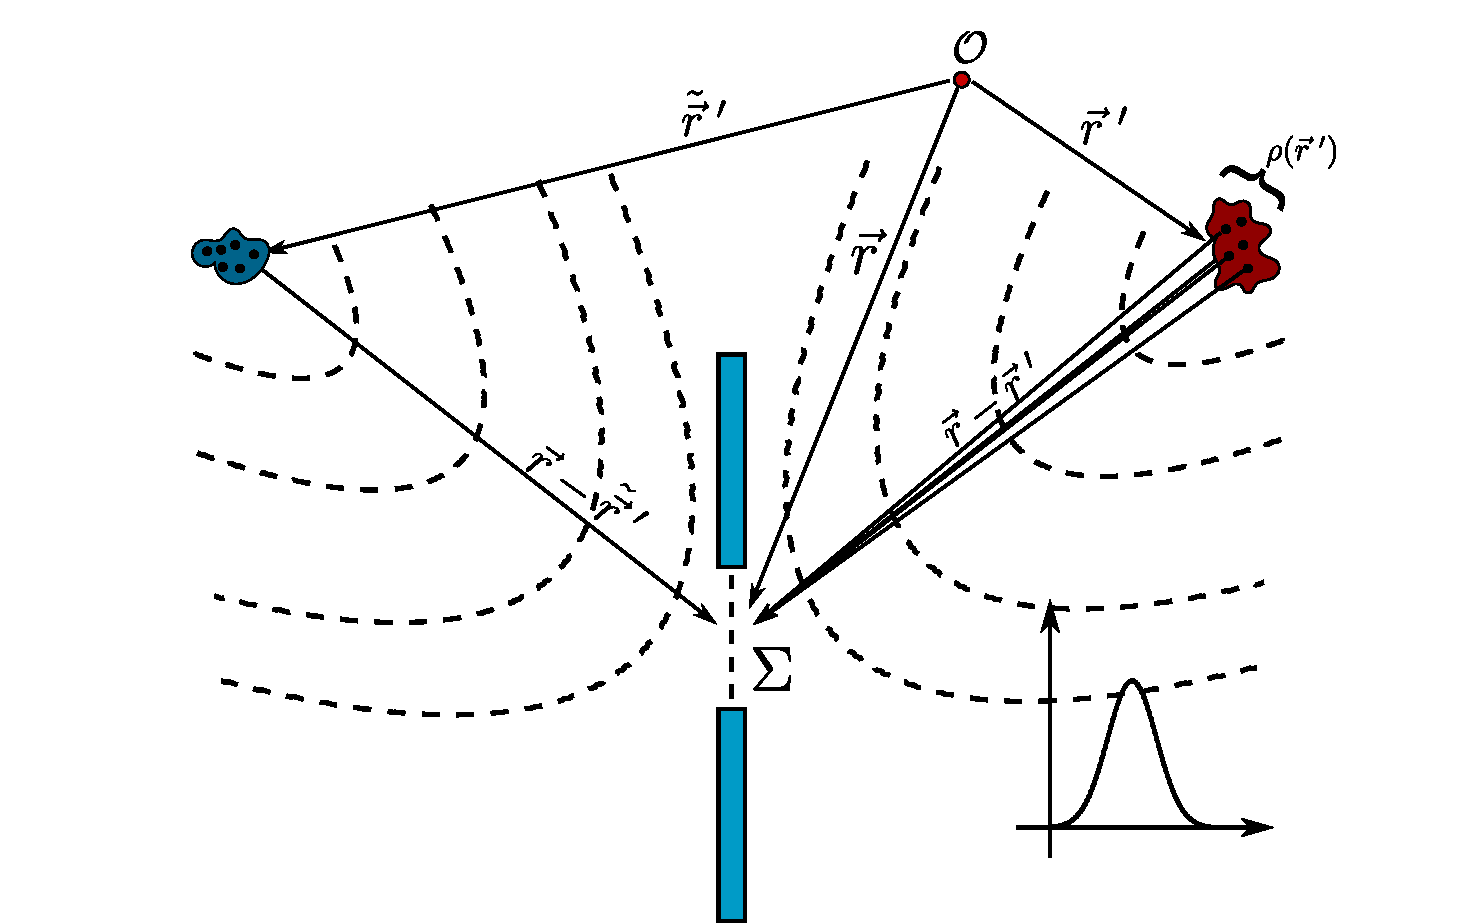
\includegraphics[width=0.5\textwidth]{Capitulo 8/Figuras/ftparabol.pdf}}
    \caption{$(a)$ Problema de Green usando una distribución $\delta$ de Dirac. $(b)$ Problema propuesto para una distribución arbitraria.}
    \label{fuentes}
    \end{figure}
     
    respectivamente, la expresión $\ref{intgreen}$ se reduce a:
    
    \begin{equation}
        U(r) = \frac{1}{4\pi} \int_{\Sigma} U \frac{\partial G_{-}}{\partial n} ds
    \end{equation}
    
    lo que da lugar a la fórmula de Rayleigh-Sommerfeld del principio de Huygens-Fresnel. \\
    Ahora bien, dado que nuestra premisa es que una onda electromagnética no puede definirse en un solo punto, sino distribuirse en una vecindad $v(\vec{r})$ $\subseteq $ $V$ de un punto definido por $\vec{r}$, la distribución de Dirac debe ser reemplazada por otra distribución que nos permita considerar el campo en la vecindad $v(\vec{r})$ como una constante, $U(v(\vec{r})) = U(\vec{r})$ [Fig. $\ref{ftparabol}$]. \\
    
    Por lo tanto, se propone, en lugar de la condición de Green $[Eq. (\ref{condgreen})]$, una nueva condición
    
    \begin{equation}
        (\nabla^{2} + k^{2})'\mathcal{G}_{\pm}(\vec{r}, \vec{r'}) = \rho (\vec{r} - \vec{r'}) \pm \rho(\vec{r} - \widetilde{\vec{r'}})
        \label{condgreen2}
    \end{equation}
    
    donde la expresión
    
    \begin{equation}
        \int_{V} U(\vec{r'}) \underbrace{(\nabla ^{2} + k^{2})' \mathcal{G} _{\pm}}_{\textstyle \rho(\vec{r} - \vec{r'})} dv' = U(v(\vec{r})) = U(\vec{r})
        \label{intgreen2}
    \end{equation}
    
    se mantiene. Recuerde que la integral se calcula en la región $V$ [lado derecho de la figura (\ref{fuentes})], donde la fuente del espejo auxiliar no afecta el resultado. \\
    
    Notemos que si colocamos las fuentes puntuales en pares (uno en la región donde se mide el campo y otro en la imagen especular), un par tras otro hasta formar un cúmulo [Fig. $\ref{ftparabol}$], entonces $\rho$ se puede escribir en base a las distribuciones de Dirac, y se puede elegir que la función $G_{\pm}$ o su derivada sean cero en el plano $(\Sigma)$ que cumpla las condiciones de Dirichlet o Neumann. Es decir, se puede elegir $\mathcal{G}(\Sigma) = 0$ o $\frac{\mathcal{G}}{n} (\Sigma) = 0$, y luego el campo se puede resolver para una vecindad de volumen $v(\vec{r})$ (del orden de la longitud de onda).
    La función $\mathcal{G}_{\pm}(\vec{r}, \vec{r'})$, que es solución de la Ec. (\ref{condgreen2}), ya no es una onda esférica y se puede escribir en la forma
    
    \begin{equation}
        (\nabla^{2} + k^{2})'\mathcal{G}(\vec{r}, \vec{r'}) = \int_{v} \rho(\vec{r}'' - \vec{r}) [\delta(\vec{r}'' - \vec{r'}) \pm \delta(\vec{r}'' - \widetilde{\vec{r'}})] d\vec{r}''
    \end{equation}
    
    lo que significa que $\mathcal{G}$ está compuesto por fuentes puntuales a lo largo de la vecindad $V$, es decir, un volumen de distribuciones de Dirac.
    Entonces la solución para el campo $U$ está dada por
    \begin{equation}
        U(r) = \frac{1}{4\pi} \int_{\Sigma} U \frac{\partial \mathcal{G}_{-}}{\partial n} ds
    \end{equation}
    
    y $\mathcal{G}_{-}$ puede elegirse para obtener cualquier otra solución para la integral de difracción siempre que (\ref{intgreen2}) sea válida.\\
    
    Dado que la propagación de fotones que obtuvimos es esencialmente la fórmula integral de difracción de Fresnel donde las ondas no son esféricas sino paraboloidales, no pueden asociarse con una distribución Dirac $\delta$, sino con un tipo diferente de distribución como se muestra antes. Es decir, los frentes de onda paraboloidales no pueden ser producidos por fuentes puntuales, sino por fuentes con alguna dimensión. El principio de Huygens es, en este sentido, un caso particular de fuentes puntuales que funciona bien cuando, en la vecindad $v$, el campo electromagnético se puede aproximar en la teoría clásica por una fuente puntual que difracta la luz en todas las direcciones. En consecuencia, podríamos pensar en la solución de la Ec. ($\ref{condgreen2}$) de tal forma que la nueva distribución conduce a una nueva función auxiliar $\mathcal{G}_{\pm}$, donde se obtiene directamente la difracción de Fresnel. \\
    
    Se ha demostrado que la difracción de Fresnel es una solución exacta de la ecuación de onda paraxial y que la ecuación paraxial también es equivalente a la ecuación de Schrödinger dependiente del tiempo para una partícula que se mueve en un potencial bidimensional, donde la coordenada $z$ desempeña el papel del tiempo y también se ha utilizado antes para estudiar la localización transversal de la luz. Nuestro tratamiento justificaría entonces el uso de la difracción de Fresnel como propagador de cuantos de luz, ya que sugiere que el propagador puede escribirse como tal basándose en un enfoque totalmente cuántico.
    
    \subsection{Experimento de conteo de fotones}
    
    Los resultados encontrados aquí se verifican mediante la implementación de un experimento de difracción por conteo de fotones (ver Fig. $\ref{fig:experimento}$). Este fue desarrollado con la única intención de mostrar la correspondencia entre este propagador de fotones y los experimentos, lo que justifica su uso, por ejemplo, para estudiar la correlación entre fotones entrelazados.
    
    \begin{figure}[htbp]
        \centering    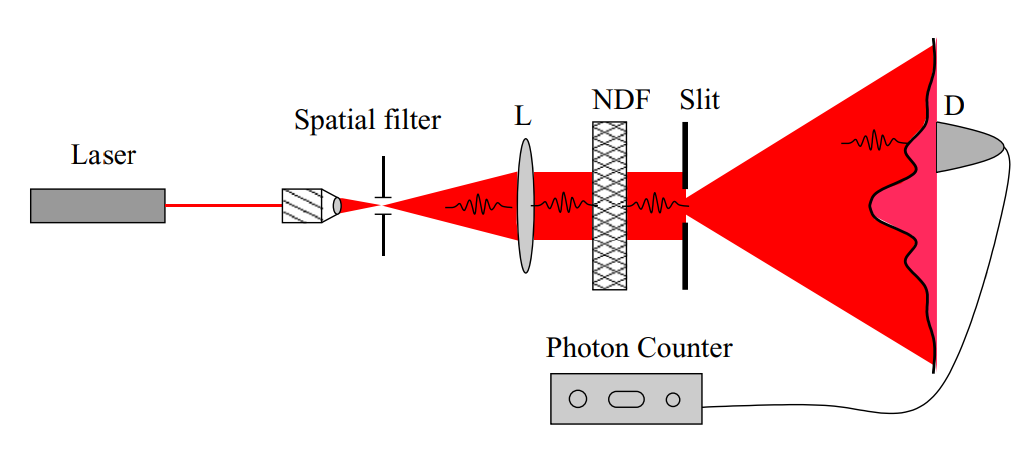
\includegraphics[width=0.8\textwidth]{Capitulo 8/Figuras/experimento.png}
        \caption{Configuración experimental.}
        \label{fig:experimento}
    \end{figure}
    
    Los resultados se verifican en un experimento de difracción con un haz láser ($\lambda$ $= 632$ $nm$) colimado con polarización lineal, el cual es atenuado mediante un arreglo de filtros de densidad neutra $(NDF)$ hasta contar un número limitado de fotones, y luego el haz es difractado por una rendija rectangular de $1905$ $\mu m$. La difracción se realiza en propagación en el espacio libre, a una distancia de $96,84$ $cm$ de la rendija hasta un contador de fotones del fotodiodo de avalancha $(D)$, cuyo diámetro es de $50$ $\mu m$. Los datos se toman durante un tiempo de $10$ $ms$ escaneando el campo difractado. \\
    
    El ajuste correcto entre los datos experimentales y el propagador de fotones según la ecuación ($\ref{eq:fresnelclasica}$) (ver Fig. $\ref{fig:dataexp}$) revela que la representación $q$ de un estado del campo puede usarse como guía para estudiar la propagación de fotones.
    
    
    \subsection{Simulación de la distribución de probabilidad para la propagación de fotones únicos}
    
    \begin{figure}[htbp]
        \centering    
        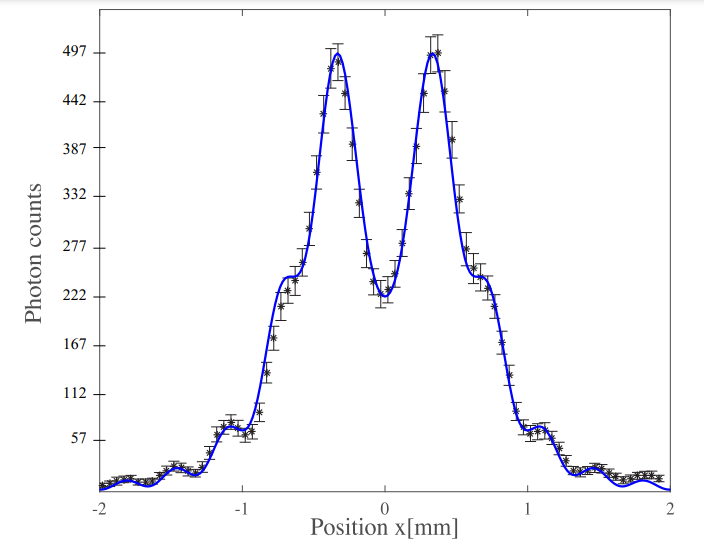
\includegraphics[width=0.7\textwidth]{Capitulo 8/Figuras/dataexp.png}
        \caption{Los datos experimentales se superpusieron a la curva azul que es la densidad de probabilidad normalizada, $\left | \Psi (x,z) \right |^{2}$, obtenido por simulación computacional.}
        \label{fig:dataexp}
    \end{figure}
    
    Es muy interesante explorar cómo evoluciona la distribución de densidad de probabilidad a medida que aumenta la distancia del plano de observación en el experimento de doble rendija. Aquí se muestra una simulación para varios planos de observación usando el propagador en Eq. ($\ref{eq:FRFT}$). A medida que el orden de la $FRFT$ se aproxima a $\alpha = \pi /2$, la distribución de densidad de probabilidad cambia hasta que alcanza el patrón de difracción de Fraunhofer característico, como se muestra en la Fig. $\ref{fig:simulacion}$. Este es un interferómetro de Young que utiliza haces gaussianos como fuentes con cintura $1/e^{2}$ radio de $0,6$ $mm$ y separación pico a pico de $4$ $mm$. Las densidades de distribución se trazan desde $\alpha = 0,8 \pi /2$ hasta $\alpha = \pi /2$ en relación con la distancia de propagación $z$.
    
    \begin{figure}[htbp]
        \centering    
        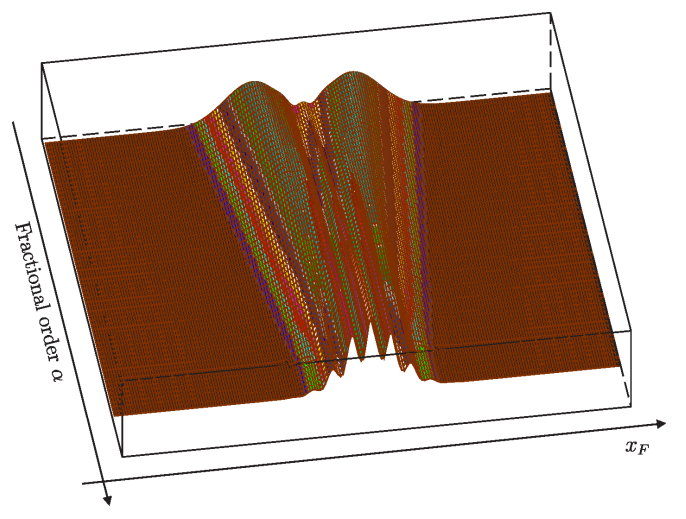
\includegraphics[width=0.7\textwidth]{Capitulo 8/Figuras/simulacion.png}
        \caption{Simulación de varias distribuciones de densidad de probabilidad a una distancia $z$.}
        \label{fig:simulacion}
    \end{figure}
    
    
    Aquí, el uso de la integral de difracción de Fresnel o, de manera equivalente, la transformada de Fourier fraccionaria ahora está fundamentalmente justificado para la propagación de un solo fotón. Nuestro tratamiento concuerda con las distribuciones de densidad de probabilidad encontradas experimentalmente por Kocsis et al. En el que pudieron construir trayectorias clásicas para fotones individuales en el interferómetro de doble rendija mediante una medición débil del momento sin destruir la interferencia. Es decir, la conclusión general, donde esas trayectorias representan el comportamiento promedio del conjunto de fotones, es confirmado por el resultado obtenido. \\
    
    Se ha encontrado un propagador de fotones que toma la forma de la integral de difracción de Fresnel clásica, mediante la estrecha conexión entre ambas y la transformada fraccionaria de Fourier. Se mostró que el observable $q$, debidamente escalado, corresponde a una posición observable transversal a la propagación del campo y paralela a la polarización del campo eléctrico. \\
    Esto significa que en el límite para un gran número de cuantos, la intensidad clásica del campo es entonces proporcional a la densidad de probabilidad, $|U(x,z)|^{2} \propto |\psi(q,t)|^{2}$, por lo que se satisface el principio de correspondencia, como se muestra en el experimento de conteo de fotones.


        \chapter{El Campo de Riemann-Silberstein}
	\thispagestyle{empty}
	\vspace*{2cm}
	\begin{center}
		{\itshape\Huge \par}
		\vspace{1cm}
		\epigraph{``El fotón no se encuentra en el campo eléctrico o en el campo magnético sino en ambos al mismo tiempo, por eso, el vector de Riemann-Silberstein es la mejor opción para describir una función de onda del fotón.''}{-- Iwo Bialynicki-Birula }
	\end{center}
	\clearpage

	\input{Capitulo 9/cap9.tex}

    \chapter{Un modelo del fotón}
    	\thispagestyle{empty}
    	\vspace*{2cm}
    	\begin{center}
    		{\itshape\Huge \par}
    		\vspace{1cm}
    		\epigraph{Por el resto de mi vida, voy a reflexionar sobre lo que es la luz}{Albert Einstein}
    	\end{center}
    	\clearpage

    	\section{Necesidad de plantear un modelo alternativo}

Uno de las etapas fundamentales que tuvo el desarrollo del entendimiento del fotón, fue la cuantización de la radiación llevada a cabo por Albert Einstein, de manera que ahora la energía de los fotones estaba \emph{cuantizada} o discretizada de la forma $E = n\hbar\omega$, siendo $n$ un número entero que caracteriza el número de \emph{cuantos} que tiene mi fotón. De manera que, dado un fotón con energía definida, esto implicaría a su vez una frecuencia $\omega$.\\


Esto último representa un conveniente teórico para nada ignorable dentro de la construcción de una teoría cuántica de la luz, puesto que si se desea estudiar la dinámica de los estados cuánticos de los fotones, irremediablemente se hace necesaria una función de onda los caracterice. La salida más directa a ello sería mediante los armónicos de Fourier: Dado un fotón con energía $E = h\nu$, su función de onda está caracterizada por una onda plana monomodal de frecuencia $\nu$, sin embargo esto implicaría una extensión infinita tanto en tiempo como en espacio, indicando un hecho para nada coherente con la fenomenología de los fotones. 


\section{Ecuación de onda de los fotones}


Un paso absolutamente necesario si se quiere estudiar una función de onda para los fotones es justamente caracterizar la ecuación de onda que describa la dinámica de este. Para ello, se retomará el vector de Riemann-Silberstein \ref{eq:RSVector}, así como las ecuaciones de Maxwell escritas en términos de este: 

\begin{equation}
    i \partial _t \mathbf{F}(\mathbf{r},t) = c \nabla \times \mathbf{F} (\mathbf{r},t)
\end{equation}  

\begin{equation}
    \nabla \cdot \mathbf{F}(\mathbf{r},t) = 0.
\end{equation}


Retomemos nuevamente la idea de concebir al vector de Riemann-Silberstein como el campo generalizado de Maxwell para fotones, de modo que haciendo uso de la identidad vectorial $\mathbf{A}\times \mathbf{B} = -i (\mathbf{A}\cdot \mathbf{S}) \mathbf{B}$, donde las componentes del vector $\mathbf{S}$ corresponden a las matrices de espín 1 (el de los fotones), las cuales pueden trabajarse en la representación dada por: 

\begin{equation}
S_x = 
\begin{pmatrix}
0 & 0 & 0 \\
0 & 0 & -i \\
0 & i & 0
\end{pmatrix}
\quad
S_y = 
\begin{pmatrix}
0 & 0 & i \\
0 & 0 & 0 \\
-i & 0 & 0
\end{pmatrix}
\quad
S_z =
\begin{pmatrix}
0 & -i & 0 \\
i & 0 & 0 \\
0 & 0 & 0
\end{pmatrix},
\end{equation}

de manera que consecuentemente se obtiene 

\begin{equation}
    i\hbar \partial_t\mathbf{F} (\mathbf{r},t) = c\left( \mathbf{S} \cdot \dfrac{\hbar}{i}\nabla \right) \mathbf{F}(\mathbf{r},t).
\end{equation}

Es inmediato notar que la estructura de la ecuación resultante se asemeja bastante a la de una ecuación de Schrodinger caracterizada por un hamiltoniano 

\begin{equation}
    \widehat{H} = c\left( \mathbf{S} \cdot \dfrac{\hbar}{i}\nabla \right)
\end{equation}


y donde la función de onda, justamente correspondería al vector de Riemann-Silberstein $\mathbf{F}(\mathbf{r},t)$. Esto apoya fuertemente la idea de considerar a las ecuaciones de Maxwell como amplitudes de probabilidad de los fotones, siendo en esencia una primera cuantización del campo electromagnético.\\


Además, si se desea ahora partir de la relación de Einstein para la energía en relatividad especial:

\begin{equation}
    E^2 = (mc)^2 + \mathbf{p}\cdot \mathbf{p} c^2, 
\end{equation}

siendo $m=0$ puesto que los fotones no tienen masa en reposo, es posible descomponer la ecuación de la forma


\begin{equation}
    \left(\frac{E^2}{c^2} - \mathbf{p}\cdot \mathbf{p}\right) I^{(3)} = \left( \frac{E}{c} - \mathbf{p} \cdot\mathbf{S} \right)\left( \frac{E}{c} + \mathbf{p} \cdot\mathbf{S} \right)I ^{(3)}  - (\mathbf{p}\otimes\mathbf{p}) I^{(3)},
\end{equation}

donde nuevamente se han introducido las matrices de espín 1, para finalmente obtener la misma estructura de la ecuación diferencial sobre un estado $\psi(\mathbf{r},t)$:

\begin{equation}
    \label{eq:R-S}
    i\hbar \partial _t \psi (\mathbf{r},t) = c\left( \mathbf{S} \cdot \dfrac{\hbar}{i}\nabla \right) \psi(\mathbf{r},t).
\end{equation}


Indicando ahora que la ecuación mecanocuántica para los estados de fotones que estamos describiendo también es invariante relativista.\\

Asimismo, el vector de Riemann-Silberstein puede ser escrito ya sea como la suma de los campos eléctrico y magnético o como su resta, es decir:

\begin{equation}
    \mathbf{F}_{\pm} = \sqrt{\frac{\epsilon_0}{2}}(\mathbf{E}(\mathbf{r},t) \pm ic\mathbf{B}(\mathbf{r},t))
\end{equation}

siendo $\mathbf{F}_+(\mathbf{r},t) = \mathbf{F}_-^\ast(\mathbf{r},t)$. Considerando esto en la ecuación de onda \ref{eq:R-S} tenemos

\begin{equation}
    i\hbar \partial _t \mathbf{F}_\pm (\mathbf{r},t) = \pm c\left( \mathbf{S} \cdot \dfrac{\hbar}{i}\nabla \right) \mathbf{F}_\pm(\mathbf{r},t), 
\end{equation}

indicando las dos helicidades ($\pm$) de los fotones, de forma que de manera completa se debería hablar de la función de onda 

\begin{equation}
\label{F_pm}
\mathcal{F} = 
\begin{bmatrix}
\mathbf{F}_{+} \\
\mathbf{F}_{-}
\end{bmatrix}
\end{equation}

donde cada componente caracteriza un fotón con una helicidad dada. \\


\subsection{Fotones como paquetes de ondas}

Estudiar al fotón como un paquete de onda, nos permite ahondar de manera más ingeniosa la cuestión sobre la localización de un fotón con energía definida $\hbar \omega$. Recordemos la pregunta fundamental que motiva todo el desarrollo mostrado en este capítulo: ¿Cómo es posible describir una partícula localizada y con frecuencia única, si su función de onda asociada se extiende infinitamente en tiempo y espacio?. \\


Ya se ha expuesto que el vector de Riemann-Silberstein funge como función de onda para los fotones, y a su vez este mismo puede estudiarse como una composición de ondas planas monomodales efectuando una transformación de Fourier:

\begin{equation}
    \mathbf{F}(\mathbf{r},t) = \frac{1}{2\pi}\int_{\infty}^\infty \mathbf{F}(\mathbf{r},\omega)e^{-i\omega t}d\omega,
\end{equation}

de manera que, entendiendo al campo generalizado de Maxwell como un oscilador que resulta de las excitaciones vacío, podemos asociar cada onda monomodal como una oscilación obtenida del vacío cuántico, quien no tiene el inconveniente conceptual de la localización espacio-temporal (pues a priori, podría tener extensión infinita). Esto motiva la solución que se propondrá a continuación, la cual corresponde a una descripción del fotón como un paquete de onda fundamentalmente policromático. \\




\noindent \emph{\textbf{Definición
}}: Entendemos por \textbf{fotón} al paquete de onda \[\psi(\mathbf{r},t) = \int_{\mathbb{R}} \xi(\mathbf{r,\nu}) e^{i2\pi \nu t} d\nu =\widetilde{\mathcal{A}}(\mathbf{r},t)e^{i2\pi \widetilde{\nu}t + \widetilde{\phi}(\mathbf{r})}, \] donde $\widetilde{\mathcal{A}} $ corresponde a la envolvente y $\widetilde{\nu}$ a la frecuencia de la portadora, junto a su respectiva fase $\widetilde{\phi}$. El espectro de $\psi(\mathbf{r},t)$ corresponde a la densidad espectral de potencia instantánea $^{w}S(\nu)$. Se dice entonces que el fotón tiene una energía $E = h\widetilde{\nu}$, y su localización se encuentra dentro del paquete de onda con una probabilidad dada por la envolvente.   \\ \\

\noindent \emph{\textbf{Densidad espectral de potencia (DEP):}} Función matemática que proporciona información sobre la distribución de la energía de una señal sobre su espectro. Para un proceso aleatorio $^w U(\nu)$, su DEP asociada se entiende como:

\begin{equation}
    ^w S(\nu) = \lim_{T\rightarrow0} \frac{|\mathcal{F}[^wU_{X}]|^2}{T},
\end{equation}

\noindent con $^wU_{X} = U(t)\Pi(\frac{t}{T})$.\\ 


\noindent \textbf{De función policromática a paquete de onda}: Esto es posible gracias al análisis de Fourier de una señal analítica $f_{A} = f(x) + if_{H}(x)$, de la forma:

\begin{equation}
    f_{A}(x) = \int_{\mathbb{R}} F_A(x')e^{+i2\pi xx'} dx' = \int_{\mathbb{R}} \widetilde{F_A}(x') \ast\delta (x'-\widetilde{x}')  e^{+i2\pi xx'} dx' = \widetilde{f_{A}}(x) e^{+i2\pi x\widetilde{x}'}
\end{equation}

\noindent donde trasladamos la función $F_{A} (x')$ en el espectro de Fourier a bajas frecuencias con una convolución y luego aplicamos $\mathcal{F}[f\cdot g] = F \ast G$. Esta última podemos escribirla en notación polar $\widetilde{f}_{A} = \widetilde{A}(x) e^{i\widetilde{\phi}(x)}$. De modo que tenemos, para nuestra señal analítica: \\

\begin{equation}
    f_{A} = \widetilde{A}(x)e^{i[\widetilde{\phi}(x) + 2\pi x \widetilde{x}' ]}.
\end{equation}


Ahora bien, conviene preguntarnos, ¿Cómo emerge el estado del fotón?, la respuesta reside en el vacío. Podemos pensar en un operador de creación $\hat{b}^{\dagger}(\omega) |0\rangle = |0_{\omega}^{\uparrow}\rangle$, el cuál toma instantáneamente uno de los modos de vibración del vacío cuántico con frecuencia $\omega$. De este modo, el estado cuántico de un fotón, también denominados estados vibracionales del vacío.

\begin{equation}
    |\gamma\rangle = \int d\omega |0^\uparrow_{\omega}\rangle.
\end{equation}


Nuestro nuevo operador de creación se relaciona con el de creación $\hat{a}^\dagger$ de toda la vida de la forma: 

\begin{equation}
    \hat{b}^{\dagger}(\omega) = \xi \hat{a}^\dagger(\omega) \rightarrow \quad |\gamma \rangle = \int d\omega \xi (\omega)\hat{a}^\dagger(\omega)|0\rangle .
\end{equation}


Esto implica que a nivel fundamental los fotones son de naturaleza policromática, lo cual iría de la mano mediciones experimentales de \emph{bandas} en lugar de \emph{lineas} de emisión para los átomos en una configuración dada. En este orden de ideas, se ve necesario introducir los estados excitados $|e\rangle$ y los estados base $|g\rangle$ de un átomo, los cuales se definen como 

\begin{equation}
    \label{exc}
    |e\rangle_{\Omega} = \int d\omega [g_e (\omega)]^{1/2}\Omega_+ (\omega)|g\rangle.
\end{equation}


\begin{equation}
    \label{bas}
    |g\rangle_{\Omega} = \int d\omega [g_g (\omega)]^{1/2}\Omega_- (\omega)|e\rangle,
\end{equation}

donde $\Omega_+ = |e\rangle \langle g|$ se puede entender como un operador de transición electrónica de estado base a excitado y  $\Omega_- = |g\rangle \langle e| = \Omega_+^\dagger$ el operador de transición de estado excitado a base. De manera que \ref{exc} y \ref{bas} están caracterizando a los estados $|e\rangle$ y $|g\rangle$ cómo bandas multimodales moduladas por las funciones de peso $ [g_e (\omega)]^{1/2}$ y $ [g_g (\omega)]^{1/2}$, siendo su producto $g(\omega) = [g_e (\omega)]^{1/2}  [g_g (\omega)]^{1/2}$ el equivalente al perfil de densidad espectral de la fuente. Esto último nos permite caracterizar qué tipo de fotones van a favorecer una transición electrónica dada, puesto que la tasa de transición va a estar relacionada con qué tan similares resulta el perfil de densidad espectral de la fuente con la densidad espectral de la radiación, es decir del paquete de onda del fotón. \\

\subsection{Estados Coherentes de los paquetes de onda}


Ya se ha definido el modelo del fotón que se está planteando, en donde hemos resaltado el papel que tiene el carácter multimodal del fotón en su interacción con una transición electrónica arbitraria. Sin embargo quedan queda aún sin definir qué se va a entender por fase cuántica del estado del fotón y la helicidad, los cuales son esenciales para entender el mecanismo de la emisión estimulada de los fotones y su diferencia con la emisión espontánea. Para ello vamos a emplear con un tipo de estados ampliamente trabajados en óptica cuántica: Los estados coherentes.\\



Dada la función de onda $|\psi_{\alpha} \rangle$, tenemos el \emph{paquete de ondas de estados coherentes}:

\begin{equation}
    | \psi_{\alpha} \rangle = \Sigma_{\sigma} \int  \frac{Vd^3k}{(2\pi)^3} \psi_{\sigma} (k) |\alpha_{\sigma} \rangle. 
\end{equation}

donde $\sigma$ es la helicidad y $|\alpha\rangle$ un estado coherente entendido como 


\begin{equation}
\left| \alpha_{\sigma}(\mathbf{k}) \right\rangle \equiv \hat{D}(\alpha_{\sigma}(\mathbf{k})) \left| \text{vac} \right\rangle 
= e^{-\frac{1}{2} |\alpha_{\sigma}(\mathbf{k})|^2} 
\sum_{n=0}^{\infty} \frac{\left( \alpha_{\sigma}(\mathbf{k}) \, \hat{a}^{\dagger}_{\sigma}(\mathbf{k}) \right)^n}{n!} 
\left| \text{vac} \right\rangle
\end{equation}




Queremos que en un espacio de Fock, esta representación siga denotando un cuanto de fotón, de modo que imponemos:

\begin{equation}
    \langle\psi_{\alpha} | \hat{N} | \psi_{\alpha} \rangle  =  \Sigma_{\sigma} \int  \frac{Vd^3k}{(2\pi)^3} |\psi_{\sigma} (k)|^2 |\alpha_{\sigma} (k)|^2  \equiv 1,
 \end{equation}


por la condición de normalización tenemos 

\begin{equation}
    \langle \psi_{\alpha}| \psi_{\alpha} \rangle = \Sigma \int \frac{V d^3k}{(2\pi)^3} \psi^\ast_{\sigma}\psi_{\sigma}(k) = 1
\end{equation}

por lo que necesariamente $\alpha_{\sigma} = e^{i\theta_{\sigma} (k)}$. De esta manera tenemos una expresión para el estado del fotón que incluye la fase cuántica:

\begin{equation}
    | \psi_{\theta} \rangle = \Sigma_{\sigma} \int  \frac{Vd^3k}{(2\pi)^3} \psi_{\sigma} (k) |e^{i\theta_{\sigma}(k)} \rangle. 
\end{equation}

Aquí podemos resaltar la ventaja que nos trae trabajar sobre representación, al emplear el espacio de estados coherentes podemos acceder a una distribución de fase bien localiza
\begin{equation}
    P(\phi) = \frac{1}{2\pi}|\langle \phi| \psi_{\theta} \rangle|^2,
\end{equation}

a diferencia de si trabajáramos simplemente en el espacio de Fock, en donde la distribución de fase es completamente uniforme para todos ángulos posibles, $P(\phi) = \frac{1}{2\pi}$. \\



Si hallamos el valor esperado del hamiltoniano: 

\begin{equation}
    \langle\Psi_\theta | \widehat{H}| \psi_\theta \rangle     = \Sigma_\sigma \int\frac{Vd^3k}{(2\pi)^3} \hbar\omega_\mathbf{k} \psi^\ast _\sigma (\mathbf{k)}\psi _\sigma (\mathbf{k)}. 
\end{equation}

encontramos que la función de peso $\psi$ caracteriza el valor esperado de la energia del estado del fotón, por lo que ya tenemos una manera apropiada de caracterizar las tres cantidades fundamentales de un estado de fotón: Su energía (asociada a su densidad de potencia espectral), su helicidad y su fase.\\

Recordemos que ya se ha descrito anteriormente una ecuación de onda para estos fotones, que estando aún en un espacio de estados coherentes debe seguir satisfaciéndolo. Para ello, consideramos ahora el vector de Riemann-Silberstein elevado a estatus de operador, y lo escribimos en términos de las dos helicidades del fotón:

\begin{equation}
    \hat{\Psi}(\mathbf{r},t)^{\pm} = \left(\frac{\epsilon_0}{2} \right)^{1/2} \left(\hat{\mathbf{E}}^\pm(\mathbf{r},t) + ic\hat{\mathbf{B}}^\pm(\mathbf{r},t) \right),
\end{equation}

de manera que podemos hallar las funciones de onda para el paquete de onda de estados coherentes en las helicidades (+) y (-) a través de los elementos diagonales del operador de campo entre el estado del fotón y el vacío.

\begin{equation}
    \Psi_\theta ^+ (\mathbf{r},t) = \langle 0| \widehat{\Psi}^+(\mathbf{r},t) | \psi^+ _\theta\rangle
\end{equation}

y 
\begin{equation}
    \Psi_\theta ^- (\mathbf{r},t)= \langle \psi_\theta| \widehat{\Psi}^- (\mathbf{r},t) | 0\rangle,
\end{equation}



de manera que ahora garantizamos que nuestra función de onda para el fotón satisface la ecuación mecanocuántica hallada en \ref{eq:R-S}. En este sentido, las soluciones que se obtienen son

\begin{equation}
    \Psi_\theta ^+(\mathbf{r},t) = i\int \frac{Vd^3k}{(2\pi)^3} \Psi_{+} \sqrt{\hbar\omega_{\mathbf{k}}} e^{i(\mathbf{k} \cdot \mathbf{r} - \omega_{\mathbf{K}}t )}e^{i\theta_+(\mathbf{k)}}
\end{equation}

y
\begin{equation}
    \Psi_\theta ^-(\mathbf{r},t) = -i\int \frac{Vd^3k}{(2\pi)^3} \Psi_{-} \sqrt{\hbar\omega_{\mathbf{k}}} e^{-i(\mathbf{k} \cdot \mathbf{r} - \omega_{\mathbf{K}}t )}e^{-i\theta_+(\mathbf{k)}}.
\end{equation}

y con ello una función de onda completa análoga a \ref{F_pm}.\\

\subsection{La emisión de fotones como estados paquetes de onda coherentes}


Ahora bien, el siguiente paso de relevancia consistiría en aplicar esta idea del fotón como paquete de onda en la interacción luz-materia, con el fin de dar una descripción de los mecanismos de emisión espontánea y estimulada (aunque a priori podría extenderse a cualquier fenómeno de absorción y emisión). Para ello, un primer paso consistiría en caracterizar nuestro hamiltoniano de interacción tipo Jaynes-Cummings \cite{Jaynes-Cummings}:

\begin{equation}
    \label{H-multimodal}
    \widehat{H}^{(I)} = \Sigma_{j,\sigma}C_{j,\sigma} \left(\widehat{\Omega}_+ \widehat{a}_{j,\sigma,\theta} + \widehat{\Omega}_-\widehat{a}^\dagger_{j,\sigma,\theta}  \right),
\end{equation}


donde las constantes $C_{j,\sigma}$ indican la probabilidad de que el átomo absorba o emita un paquete de ondas con modos $j$ y helicidad $\sigma$, de igual forma se tienen los operadores de transición electrónica $\widehat{\Omega}_{\pm}$, y los operadores escalera asociados al campo electromagnético

\begin{equation}
    \widehat{a}^\dagger_{j,\sigma,\theta} \equiv\int \frac{Vd^3k}{(2\pi)^3} U_{j}^{(\sigma)}(\mathbf{k})\widehat{D}(e^{i\theta_{\sigma}(\mathbf{k})})
\end{equation}
y
\begin{equation}
    \widehat{a}_{j,\sigma,\theta} \equiv\int \frac{Vd^3k}{(2\pi)^3} U_{j}^{(\sigma)}(\mathbf{k})\widehat{D}^\dagger(e^{i\theta_{\sigma}(\mathbf{k})}),
\end{equation}

los cuales siguen la misma idea de un operador de creación y aniquilación de carácter multimodal modulado por $U_j^{\sigma}(\mathbf{k})$), utilizando el operador de desplazamiento tal que, aplicado sobre vacío obtenemos 

\begin{equation}
\hat{a}^{\dagger}_{j, \sigma, \theta} | \text{vac} \rangle 
= \int \frac{V \, d^3 \mathbf{k}}{(2\pi)^3} \, U^{(\sigma)}_j(\mathbf{k}) 
\, \hat{D} \left( e^{i \theta_{\sigma}(\mathbf{k})} \right) | \text{vac} \rangle = |1_{j, \sigma, \theta} \rangle,
\end{equation}

representando así al estado cuántico de un fotón con una energía caracterizada por los modos j, helicidad $\sigma$ y fase $\theta$. Cabe resaltar que  $U_j^{\sigma}(\mathbf{k})$) satisface 

\begin{equation}
\label{U-dirac}
\sum_j U^{(\sigma)}_j(\mathbf{k}') U^{(\sigma)}_j(\mathbf{k}) 
=  \delta_{j j'}, 
\quad
\int \frac{V \, d^3 \mathbf{k}}{(2\pi)^3} 
\left( U^{(\sigma)}_{j'}(\mathbf{k}) \right)^{\dagger} U^{(\sigma)}_j(\mathbf{k}) 
= (2\pi)^3 \delta(\mathbf{k}' - \mathbf{k}),
\end{equation}






de modo que podemos hallar la relación de conmutación entre nuestros operadores escalera multimodales

\begin{equation}
\left[ \hat{a}_{j, \sigma, \theta}, \hat{a}^{\dagger}_{j', \sigma', \theta} \right] 
= \delta_{j j'} \delta_{\sigma \sigma'}.
\end{equation}

Dicho esto, tenemos entonces el caso de la emisión espontánea en donde el estado inicial del sistema $\psi _i = |e\rangle|vac\rangle$, es decir se tiene un electrón en estado excitado y un campo electromagnético en ausencia de fotones, es decir, tenemos el vacío cuántico. De manera que aplicando el hamiltoniano de interacción \ref{H-multimodal}:

\begin{equation}
    |\psi_f \rangle = H^{(I)} |\psi_i\rangle = \Sigma_{j,\sigma} C_{j,\sigma}|g\rangle |1_{j,\sigma,\eta}\rangle,
\end{equation}


en donde es claro que la fase $\eta$ resulta ser de carácter arbitrario puesto que en el estado del vacío la fase de un estado coherente se encuentra completamente deslocalizada. Asimismo, los modos y la helicidad dependerán del estado de la fuente, de modo que el estado final del sistema está en una superposición de todos los posibles paquetes de onda que pueden emitirse para efectuar la transición mostrada.\\


En este orden de ideas, se aborda ahora la situación de la emisión estimulada de fotones, en la cual se tiene como estado inicial del sistema a $ |\psi_i \rangle = |e\rangle  | |1_{j,\sigma,\theta} \rangle$. De manera que la interacción esta dada por

\begin{equation}
    |\psi_f \rangle = H^{(I)} |\psi_i\rangle = \Sigma_{j,\sigma} C_{j,\sigma}|g\rangle |2_{j,\sigma,\theta}\rangle,
\end{equation}

donde el fotón emitido hereda las mismas propiedades $j, \sigma, \theta$ del fotón que estimuló la emisión, ya que si se sigue la relación \ref{U-dirac}, se tiene que el operador de creación actuará solo para un modo, helicidad y fase específico:

\begin{equation}
\widehat{a}^\dagger_{j',\sigma',\theta'} |1_{j,\sigma,\theta}\rangle = |2_{j,\sigma,\theta}\rangle \delta_{jj'}\delta_{\sigma \sigma'},
\end{equation}


por lo que los dos fotones resultantes en la emisión resultan ser idénticos. Esta es la idea principal que va a dar respuesta a qué es la coherencia cuántica de campo electromagnético, puesto que si se sigue la teoría desarrollada por Roy Glauber para la coherencia de los fotones \cite{Glauber-Coherencia}, se dice que el campo será completamente coherente (a primer orden, pero puede extenderse la idea a orden $n$) cuando el \emph{grado de coherencia} sea igual a uno, es decir: 

\begin{equation}
    \label{grad_coher}
     |g^{(1)}(x_1,x_2)| =\frac{|G^{(1)}(x_1,x_2)|}{|G^{(1)}(x_1,x_1)G^{(1)}(x_2,x_2)|^{1/2}} = 1,
 \end{equation}


 donde $G^{(1)} = \langle1_{j,\sigma,\theta}| \widehat{E}^{(-)}(x_1) \widehat{E}^{(+)}(x_2) |1_{j,\sigma,\theta}\rangle $ es la denominada \emph{función de coherencia a orden 1}. Vemos que para ello era necesario caracterizar la función de onda de los fotones que componen el campo, tarea que ya se ha descrito hasta ahora, de modo que la función de coherencia obtenida en este caso es 

\begin{equation}
G^{(1)}(x_1, x_2) = \sum_{\sigma} \int \frac{V \, d^3 \mathbf{k}}{(2\pi)^3} 
\frac{\hbar \omega_{\mathbf{k}} \left| U^{(\sigma)}_j(\mathbf{k}) \right|^2}{2 \epsilon_0 V} 
\, e^{i \left[ \mathbf{k} \cdot (\mathbf{r}_2 - \mathbf{r}_1) - \omega_{\mathbf{k}} (t_2 - t_1) \right]},
\end{equation}

quien satisface la condición de coherencia a primer orden dada en \ref{grad_coher}. Es decir, que las correlaciones en dos puntos $x_1$y $x_2$ del campo cuántico electromagnético surgen de las similitudes en las estadísticas de los fotones que lo componen: Si un campo esta compuesto por $n$ fotones idénticos, las estadísticas que describen sus modos, helicidades y fases serán las mismas, por lo que el campo se dice que será completamente coherente puesto que sus estadísticas están en completa correlación. Si por el contrario todos los $n$ fotones son diferentes, las estadísticas de sus obervables principales también lo son y entonces el campo será completamente no coherente, o lo que es lo equivalente, la correlación estadística será nula. \\ 


	
	\bibliography{referencias}
	
\end{document}
